\documentclass[12pt,a4paper]{article}
%DIF LATEXDIFF DIFFERENCE FILE
%DIF DEL old.tex   Tue Nov 24 20:56:58 2026
%DIF ADD new.tex   Tue Nov 24 20:56:58 2026
\usepackage[left=24mm,right=24mm,top=23mm,bottom=23mm]{geometry}
\usepackage{nature_reading}
%DIF 4a4
\extrafloats{128} %DIF >
%DIF -------
\usepackage{setspace,lineno,etoolbox}
\AtBeginEnvironment{thebibliography}{\singlespacing}
% Generated from pinned audit evidence.
\newcommand{\TrainSeconds}{361.6}
\newcommand{\TrainMemory}{0.543}
\newcommand{\FirstIdentity}{1.17}
\newcommand{\FirstShuffled}{1.17}
\newcommand{\FirstZero}{0.00}
\newcommand{\BlockIdentity}{0.586}
\newcommand{\BlockGain}{0.098}
\newcommand{\BlockLow}{0.000}
\newcommand{\BlockHigh}{0.307}
\newcommand{\BlockFone}{0.320}
\newcommand{\RunDecision}{reject}

% Generated from the pinned V54 audit; no fitted presentation values.
\newcommand{\DensitySeconds}{207.8}
\newcommand{\DensityMemory}{0.400}
\newcommand{\DensityNll}{15.219}
\newcommand{\DensityShuffledNll}{15.254}
\newcommand{\DensityAdvantage}{0.0355}
\newcommand{\DensityLow}{-0.1014}
\newcommand{\DensityHigh}{0.1693}
\newcommand{\DensityIdentity}{1.562}
\newcommand{\DensityFone}{0.350}
\newcommand{\DensityCopyFone}{0.99949}
\newcommand{\DensityDecision}{reject}

% Generated from the locked V55 matched audit.
\newcommand{\JointNll}{7.026}
\newcommand{\ControlNll}{7.579}
\newcommand{\JointNllGain}{0.553}
\newcommand{\JointNllLow}{0.450}
\newcommand{\JointNllHigh}{0.665}
\newcommand{\JointTime}{342.4}
\newcommand{\ControlTime}{218.0}
\newcommand{\JointMemory}{0.648}
\newcommand{\ControlMemory}{0.400}
\newcommand{\JointSampleFone}{0.362}
\newcommand{\JointPrefixGain}{0.185}
\newcommand{\JointDecision}{reject}

% Generated from unchanged V56 report.
\newcommand{\BeamAccuracy}{11.621}
\newcommand{\BeamShuffled}{9.863}
\newcommand{\GreedyAccuracy}{8.252}
\newcommand{\BeamGain}{3.369}
\newcommand{\BeamGainLow}{2.351}
\newcommand{\BeamGainHigh}{4.412}
\newcommand{\BeamHistoryGain}{1.758}
\newcommand{\BeamHistoryLow}{0.966}
\newcommand{\BeamHistoryHigh}{2.552}
\newcommand{\BeamRepeat}{25.446}
\newcommand{\TargetRepeat}{0.112}
\newcommand{\BeamSeconds}{269.3}
\newcommand{\BeamMemory}{0.154}
\newcommand{\BeamDecision}{reject\_decoder}

% Generated from the completed V57 audit.
\newcommand{\QaExact}{3.906}
\newcommand{\QaFone}{15.718}
\newcommand{\QaBlankExact}{0.391}
\newcommand{\QaBlankFone}{5.553}
\newcommand{\QaControlExact}{0.000}
\newcommand{\QaControlFone}{6.582}
\newcommand{\QaQuestionGain}{10.165}
\newcommand{\QaQuestionLow}{7.043}
\newcommand{\QaQuestionHigh}{13.371}
\newcommand{\QaPairExact}{0.254}
\newcommand{\QaMotor}{100.000}
\newcommand{\QaSeconds}{278.572}
\newcommand{\QaMemory}{1.053}
\newcommand{\QaControlSeconds}{269.126}
\newcommand{\QaControlMemory}{1.049}
\newcommand{\QaDecision}{reject\_reading\_model}

% Generated from the fixed autonomous verification receipt.
\newcommand{\CodecLanguageFOne}{32.671}
\newcommand{\CodecLanguageBlankFOne}{19.508}
\newcommand{\CodecLanguageQuestionGain}{13.163}
\newcommand{\CodecLanguageCILow}{10.933}
\newcommand{\CodecLanguageCIHigh}{15.730}
%DIF 86a87-88
 %DIF >
% Reading abstract for the cumulative study. %DIF >
%DIF -------




\onehalfspacing\linenumbers
%DIF PREAMBLE EXTENSION ADDED BY LATEXDIFF
%DIF CFONT PREAMBLE %DIF PREAMBLE
\RequirePackage{color}\definecolor{RED}{rgb}{1,0,0}\definecolor{BLUE}{rgb}{0,0,1} %DIF PREAMBLE
\DeclareOldFontCommand{\sf}{\normalfont\sffamily}{\mathsf} %DIF PREAMBLE
\providecommand{\DIFadd}[1]{{\protect\color{blue} \sf #1}} %DIF PREAMBLE
\providecommand{\DIFdel}[1]{{\protect\color{red} \scriptsize #1}} %DIF PREAMBLE
%DIF SAFE PREAMBLE %DIF PREAMBLE
\providecommand{\DIFaddbegin}{} %DIF PREAMBLE
\providecommand{\DIFaddend}{} %DIF PREAMBLE
\providecommand{\DIFdelbegin}{} %DIF PREAMBLE
\providecommand{\DIFdelend}{} %DIF PREAMBLE
\providecommand{\DIFmodbegin}{} %DIF PREAMBLE
\providecommand{\DIFmodend}{} %DIF PREAMBLE
%DIF IDENTICAL PREAMBLE %DIF PREAMBLE
\providecommand{\DIFaddFL}[1]{\DIFadd{#1}} %DIF PREAMBLE
\providecommand{\DIFdelFL}[1]{\DIFdel{#1}} %DIF PREAMBLE
\providecommand{\DIFaddbeginFL}{\DIFaddbegin} %DIF PREAMBLE
\providecommand{\DIFaddendFL}{\DIFaddend} %DIF PREAMBLE
\providecommand{\DIFdelbeginFL}{\DIFdelbegin} %DIF PREAMBLE
\providecommand{\DIFdelendFL}{\DIFdelend} %DIF PREAMBLE
%DIF COLORLISTINGS PREAMBLE %DIF PREAMBLE
\RequirePackage{listings} %DIF PREAMBLE
\RequirePackage{color} %DIF PREAMBLE
\lstdefinelanguage{DIFcode}{ %DIF PREAMBLE
%DIF DIFCODE_CFONT %DIF PREAMBLE
  moredelim=[il][\color{red}\scriptsize]{\%DIF\ <\ }, %DIF PREAMBLE
  moredelim=[il][\color{blue}\sffamily]{\%DIF\ >\ } %DIF PREAMBLE
} %DIF PREAMBLE
\lstdefinestyle{DIFverbatimstyle}{ %DIF PREAMBLE
	language=DIFcode, %DIF PREAMBLE
	basicstyle=\ttfamily, %DIF PREAMBLE
	columns=fullflexible, %DIF PREAMBLE
	keepspaces=true %DIF PREAMBLE
} %DIF PREAMBLE
\lstnewenvironment{DIFverbatim}[1][]{\lstset{style=DIFverbatimstyle}}{} %DIF PREAMBLE
\lstnewenvironment{DIFverbatim*}[1][]{\lstset{style=DIFverbatimstyle,showspaces=true}}{} %DIF PREAMBLE
\lstset{extendedchars=\true,inputencoding=utf8}

%DIF END PREAMBLE EXTENSION ADDED BY LATEXDIFF

\begin{document}
\noindent{\color{blue}\footnotesize Change-marked copy: additions relative to the 0f14fa3f compact-diagnosis draft are blue.}\par\medskip

{\sffamily\bfseries\DIFdelbegin %DIFDELCMD < \Large{Learning conditional language\\in continuous image space}%%%
\DIFdelend \DIFaddbegin \Large{Conditional language generation\\in glyph image space}\DIFaddend \par}\medskip Imagized Language Model Project\par\medskip
\section*{Abstract}{\DIFdelbegin \DIFdel{Written language includes forms outside standard character encodings. We investigate continuous interfaces that read }\DIFdelend \DIFaddbegin \DIFadd{Can a model learn what writing means when both the prompt }\DIFaddend and \DIFdelbegin \DIFdel{emit glyph }\DIFdelend \DIFaddbegin \DIFadd{the reply are }\DIFaddend images\DIFdelbegin \DIFdel{, }\DIFdelend \DIFaddbegin \DIFadd{? We trained a causal writer }\DIFaddend with \DIFdelbegin \DIFdel{generated pixels supplying subsequent history. Externally pretrained foundations provide inherited language knowledge; tokenizers}\DIFdelend \DIFaddbegin \DIFadd{2.12 million parameters on pictured English and Chinese books}\DIFaddend , \DIFdelbegin \DIFdel{lexical heads }\DIFdelend \DIFaddbegin \DIFadd{instructions }\DIFaddend and \DIFdelbegin \DIFdel{font rendering are absent }\DIFdelend \DIFaddbegin \DIFadd{reference questions using one consumer GPU. On held English fiction the predictive cost fell }\DIFaddend from \DIFaddbegin \DIFadd{5.66 to 2.64 bits per glyph. Exchanging }\DIFaddend the \DIFdelbegin \DIFdel{deployed answer path}\DIFdelend \DIFaddbegin \DIFadd{prompt increased it to 2.83}\DIFaddend . \DIFdelbegin \DIFdel{A restricted actor retaining 7.522B visual and contextual parameters gives sixteen clear complete literal }\DIFdelend \DIFaddbegin \DIFadd{The improvement did not translate into reliable free }\DIFaddend answers\DIFdelbegin \DIFdel{among 32 reserved questions, versus eleven for a fixed-body control}\DIFdelend . \DIFdelbegin \DIFdel{Neither arm passes its qualification}\DIFdelend \DIFaddbegin \DIFadd{The writer repeated words when asked how to conserve energy and failed to write both correct names on any of 120 external contrast pairs}\DIFaddend . \DIFdelbegin \DIFdel{A separate compact experiment freezes }\DIFdelend \DIFaddbegin \DIFadd{We then fitted }\DIFaddend a \DIFdelbegin \DIFdel{1.409B contextual body }\DIFdelend \DIFaddbegin \DIFadd{reader that could continue copying a sequence of source glyphs or switch back to free writing. On 384 human questions in English, simplified }\DIFaddend and \DIFdelbegin \DIFdel{fits image interfaces on 13}\DIFdelend \DIFaddbegin \DIFadd{traditional Chinese}\DIFaddend , \DIFdelbegin \DIFdel{785 }\DIFdelend \DIFaddbegin \DIFadd{it produced 11 }\DIFaddend complete \DIFdelbegin \DIFdel{Chinese book and question--answer sequences}\DIFdelend \DIFaddbegin \DIFadd{reference answers}\DIFaddend , \DIFdelbegin \DIFdel{covering 2.576 million target glyph positions. Two 8,172-update fits use 3.930 }\DIFdelend \DIFaddbegin \DIFadd{compared with 12 without source-position persistence }\DIFaddend and \DIFdelbegin \DIFdel{4.889 GiB peak allocated GPU memory. Both score }\DIFdelend zero \DIFdelbegin \DIFdel{complete exact QA answers out of 32 at all five checkpoints. A wider }\DIFdelend \DIFaddbegin \DIFadd{for the original }\DIFaddend writer\DIFdelbegin \DIFdel{removes a measured velocity-rank restriction without solving language}\DIFdelend . \DIFdelbegin \DIFdel{Frozen-weight diagnostics show that writing fails before generated feedback, despite near-exact codec reconstruction; additional sampling steps do not repair it}\DIFdelend \DIFaddbegin \DIFadd{No system answered both questions correctly on any of 192 unseen passages}\DIFaddend . \DIFdelbegin \DIFdel{The reader also has a measured affine target-alignment restriction}\DIFdelend \DIFaddbegin \DIFadd{Physical glyphs support measurable conditional prediction}\DIFaddend . \DIFdelbegin \DIFdel{Cold replays verify independent pixel-feedback execution for fixed cases. }\DIFdelend These \DIFdelbegin \DIFdel{results separate execution, physical }\DIFdelend \DIFaddbegin \DIFadd{experiments locate a remaining gap between recognizing local }\DIFaddend writing \DIFaddbegin \DIFadd{patterns }\DIFaddend and \DIFdelbegin \DIFdel{conditional language success. Reliable open-ended generation, historical-form transfer and }\DIFdelend \DIFaddbegin \DIFadd{using }\DIFaddend a \DIFdelbegin \DIFdel{matched-quality efficiency advantage remain unresolved}\DIFdelend \DIFaddbegin \DIFadd{question to generate a meaningful answer}\DIFaddend .}\par\bigskip
\DIFdelbegin \DIFdel{Written language is encountered as marks on paper, screens and
historical
surfaces. Its visual form carries information about script, handwriting and material history. Modern character encodings provide a powerful interface to
many such marks, but a finite inventory cannot express every damaged, transitional or unencoded form. An image-based language model could retain
that evidence throughout reading and generation, with transcription offered
as an optional output view}\DIFdelend %DIF >  Active article input; prior staged versions remain in Git and validation receipts.
\DIFaddbegin \DIFadd{Writing reaches a reader as visible marks. Script, typeface, handwriting and
damage change those marks without necessarily changing their interpretation.
Conversely, historical or unfamiliar forms may have no agreed character
identity in a chosen encoding or tokenizer. A visual language interface would
retain the marks while learning to interpret and continue them. Its intended
output is readable writing, including explanatory passages and, eventually,
attested forms absent from the model's preparation fonts. This motivation does
not establish that image representations carry more usable information per
unit of computation or reproduce human reading mechanisms. We therefore test two complementary tasks. In one, the writer must draw an English meaning absent from a classical Chinese line. In another, the exact answer occurs in an English passage, and changing the question should select a different part of the same image. The second task isolates question-dependent reading while preserving the original ink.
}

\DIFadd{Two names followed by two prices provide an attribution test. A reader can copy every digit yet give the second venue the first venue's admission price. We ask whether a relation learned from pictured English letters and Chinese characters can change an answer when the source says \emph{the former} or \emph{the latter}. We compare the same output writer with and without a reference reader, and test the reader separately on naturally occurring prose (Fig.~\ref{fig:story-mentions}).
}

\DIFadd{A price and an address can both appear in a response that calls the price the address. This provides a stronger test than matching the presence of source values. We examine whether a visual reader can identify multiple requested properties in a printed question and condition the surrounding language on which fact it is currently expressing. We measure the reader, the complete sentence and local device cost separately.
}

\DIFadd{A question can change the meaning of the requested answer while leaving every pixel of the evidence unchanged. We test this using human Chinese dialogue about venues. Speakers ask about hours, prices and locations in their own words. We provide one pictured record and ask the model to write its reply. Opposing questions on the same record, a removed question and a matched byte-input control help separate conditional reading from familiar answer wording. A second experiment asks whether names outside the learned writing palette can keep their identity and grammatical role inside an English sentence}\DIFaddend .

\DIFdelbegin \DIFdel{Pixel-based language modelling already has substantial precedents. PIXAR demonstrates autoregressive language generation in pixel space and identifies the difficulty of generating readable text\cite{pixar}. Continuous
autoregression can use a diffusion loss in place of vector quantization\cite{mar},
while Diffusion Forcing models continuous sequences under independently chosen
noise levels\cite{forcing}. These results motivate a visual language interface, but do not establish that a small glyph generator acquires linguistic knowledge or that image input automatically reduces training cost. Exact pixel factorization also }\DIFdelend \DIFaddbegin \DIFadd{The practical test is whether the same visible marks can support different answers when the question changes. A page can contain both an oracle form and a bronze form of one character, or a paragraph can mention two people who did different things. Recovering a crisp glyph shows that the writer can reproduce a mark. Selecting the right mark for the user's claim requires it to bind that claim to its evidence. We test both directions of dependence by varying the question on a fixed passage and varying the passage for a fixed question. We also ask the model to recover excised writing whose glyphs may be absent from the displayed inputs.
}

\DIFadd{A classical character can name an action in one line and stand for a participant in another. To test whether a visual model learns this distinction, we ask it to draw different English words for the same central glyph. We measure what it writes when given the location and what it writes when it must first find that location by reading a question.
}

\DIFadd{A second question is how much of a reader's language knowledge depends on its input alphabet. We test this by removing the lexical lookup from a pretrained Chinese reading model, learning a continuous input map on glyph images and returning the selected source pixels. Typeface changes then probe the visual map directly. A separate recurrent writer handles requests for which the answer must be composed in a different order. This design lets us distinguish transferring existing linguistic knowledge into an image interface from acquiring that knowledge through visual training alone. A pictured question can also request two forms that occupy separate locations. Span-copying models have represented a text edit as a sequence of source selections and generated elements (}\href{https://arxiv.org/abs/2006.04771}{\DIFadd{Panthaplackel et al.}}\DIFadd{). We test this operation on physical glyphs by reversing the requested order while retaining identical evidence.
}

\DIFadd{Pixel-space language generation }\DIFaddend has established precedents\DIFdelbegin \DIFdel{in }\DIFdelend \DIFaddbegin \DIFadd{. PIXAR studies
autoregressive text generation from pixel representations and identifies
readability as a central difficulty\cite{pixar}. }\DIFaddend PixelRNN and conditional
PixelCNN \DIFdelbegin \DIFdel{\cite{pixelrnn,pixelcnn}. Masked autoregressive networks
provide normalized probabilities without a character dictionary\cite{made}. Multilingual generation from pixels has also
been studied\cite{mixar}}\DIFdelend \DIFaddbegin \DIFadd{provide normalized image-density formulations\cite{pixelrnn,pixelcnn}.
Their existence motivates a trainable visual writing distribution, but neither
an image likelihood nor a sharp glyph establishes that an answer follows its
question. Replacing a character inventory with physical image variables also
does not remove discrete computation: a binary raster and a categorical
distribution over small pixel masks are discrete representations of appearance}\DIFaddend .

\DIFdelbegin \DIFdel{Recent continuous multimodal flow models share a generative objective across
embeddings while retaining token-derived language encoders and text
decoders\cite{multimodalflow}. OCG reports rendered-question and answer-image
reasoning with teacher assistance on the restricted CLEVR task\cite{ocg}.
We focus on independent image-only inference and controlled tests linking
conditional scores to autonomous writing.
}\DIFdelend \DIFaddbegin \DIFadd{We study the coupling directly. A prompt image supplies context; a neural
writer emits a glyph image; the model rereads the actual emitted pixels before
deciding what to write next and when to stop. Typed questions may be rendered
at the input boundary, and transcription may follow completed image generation.
Neither operation supplies answer identities to the deployed writing loop.
Offline text, teachers and pretrained foundations remain permitted sources of
supervision and inherited knowledge. Independent inference therefore differs
from learning a language entirely from images without textual pretraining.
}\DIFaddend

\DIFdelbegin \DIFdel{We investigate the conditional generation problem directly. The model
receives raster history, predicts a distribution of future writing, emits
pixels and rereads those pixels. Chinese provides a demanding initial case:
stroke configurations must remain coherent while context selects among many
similar written forms}\DIFdelend \DIFaddbegin \DIFadd{The initial language setting uses Chinese writing in one canonical font and
ordered glyph cells. This isolates conditional shape generation before raw
page reading, handwriting or historical-script transfer. Earlier compact
complete-sequence fits produce zero strict complete answers at their fixed
checkpoints. The subsequent full continuation trial recomputes all 36 answer
layers while preserving frozen prompt memory, exposing complete QA and book
targets rather than only isolated first glyphs. Its five prescribed checkpoints,
paired questions, erased inputs, long continuations and retained successes
separate physical fidelity from complete language. The final model improves
some short answers relative to its initial checkpoint but fails the pilot}\DIFaddend .
\DIFdelbegin \DIFdel{The present study uses one canonical font to isolate
this coupling before introducing handwriting or historical scripts. }\DIFdelend

\DIFdelbegin \DIFdel{The experiments progress from initial raster readers and denoisers to inherited contextual bodies with separately learned glyph interfaces. The
earlier architectures provide controls. Restricted short-answer experiments evaluate the complete-glyph loop shown in Fig. ~S37; a separate compact
experiment then fits complete book and question--answer sequences and measures
all five saved checkpoints.
A controlled wider writer and frozen-weight
interventions then test the sources of failure.
The contributions are the explicit }\DIFdelend \DIFaddbegin \DIFadd{The study contributes an explicit }\DIFaddend emitted-pixel \DIFdelbegin \DIFdel{interface, controlled language tests , reproducible
single-GPU execution and measured writer/reader restrictions. None establishes a generally
usable visual language model or a from-scratch language learner. }\DIFdelend \DIFaddbegin \DIFadd{inference interface, controlled
complete-language comparisons and evidence that supplied-history writing and
one-GPU execution are insufficient qualifications. The failed full trial
motivates a separate conditional joint glyph writer. That head-only fit is
complete and fails its physical prerequisite; its original review credits
are preserved with detected blank-flag errors rather than treated as corrected
physical accuracy. The probability diagnosis in turn motivates training the
continuation state through complete-image likelihood. That full comparison
lowers source loss while increasing false blanks and failing every book group.
An actual-context probability bound identifies empty global modes, motivating
a separately registered whole-glyph ranking loss. That complete fit improves
recognized nonempty forms but fails legitimate blank targets. Exact source-image
reproduction changes little, and complete language remains unmeasured. A new
objective for blank targets passes a reset full-body computational preflight;
its complete quality comparison fails both blank conditions. A subsequent
full-context comparison tests whether allowing all inherited context weights to learn improves complete answers or book continuations.
The larger objective is useful
visual language across written forms, with historical and unencoded writing
assessed on its own provenance, shape and meaning. That objective remains open.
}\DIFaddend

\DIFaddbegin \DIFadd{To measure what the visual reader learns before it draws an answer, we also
present paired Mandarin sentences containing identical glyphs in different
orders. Each pair holds the physical inventory constant while changing the
linguistic context of the observed marks.
}

\DIFadd{A reader can answer some questions by locating a span of writing already
present on a page. Drawing a historical form absent from the prompt also
requires a reliable writer. We test these capabilities separately.
}

\DIFadd{A change of context should also change which glyph a writer expects. We
measure this dependence with passages ending in the same visible character
and compare pixel and character-indexed learning on identical training text.
}

\DIFadd{A historical caption may require alternating between an attested source shape
and modern connecting text. In contrast, a factual question can require
returning just one name from an existing passage. We examine whether a
visual reader can learn when each response is appropriate.
}

\DIFadd{An answer can be legible yet name the wrong person. We therefore ask whether placing more training weight on the first glyph changes which fact a writer selects. We test complete answers to two distinct questions asked in both Chinese and English about passages from four additional literary works.
}

\DIFadd{We next ask whether a writer can learn from the complete wrong answers it has produced itself. A writer that learns a correction on a familiar passage may still miss the corresponding distinction in another book. We compare learning on the original pairs with independent image responses to four requests on each new passage.
}

\DIFadd{Two facts in a single reply test a different ability from finding two excerpts separately. We ask for the same information in opposite orders, first allowing the writer to generate the entire reply and then letting it write around source ink selected for each question. Both tests retain the original answer pixels so that a reader can distinguish a correct statement from a list of names.
}

\DIFadd{Recent experiments with a shared image canvas report higher symbolic-reasoning accuracy when a model can write and read intermediate visual steps~\cite{chucanvas}. Here the intermediate question is supplied by the reader. By changing who performed an action while retaining both names, we can ask whether a writer uses the combination of page and question to choose its next clause.
}

\DIFadd{A conversational answer can require a word missing from the pictured passage. We therefore allow a reader to copy individual word images and to spell new words from printed shapes. Exchanging the pictured question and editing a date in the passage test whether the resulting answer follows the input. Supplying the visual features of the intended word in a separate experiment isolates spelling from deciding which word to write.
}

\DIFadd{A claim of energy efficiency requires comparison at a common level of language performance. We compare a pictured writer with a subword Transformer and then hold architecture and supervision fixed while changing only how a letter is observed. This design separates an advantage of a complete trained system from the narrower question of whether printed shape itself reduces the cost of learning.
}

\DIFadd{A book also tests whether meaning survives the writer's own first mistake. We retain the original passage during generation and exchange its distant glyphs while preserving its ending. Comparing the result with a byte reader and a count predictor measures how much the pictured context contributes to recovering the continuation.
}

\DIFadd{A torn or faded line poses a different question. If several positions are blank, the reader can begin where the neighbouring text is most informative. Paired lines of verse let us test this choice directly and distinguish recovering a printed shape from recovering the expression that belongs there.
}

\DIFadd{A familiar expression can fit the metre and still belong to another poem. We train with exchanged sources and test whether the resulting preference for authentic pairings carries over to writing an entire missing phrase in verse from another period.
}

\DIFadd{An illustrated dictionary poses a question that a continuation score cannot answer. Can a reader find the requested headword among thousands of records, then reproduce its attested forms in the order a reader asks for them? Removing that record tests whether it can also recognize a gap in the available evidence.
}


\DIFadd{A writer can copy a gloss from a dictionary without composing a new sentence. We therefore render restaurant records as cards and ask a model trained from scratch to describe them in English. In one contrast, the name, venue, food, location and nearby landmark remain the same while the family policy changes. We ask whether reading the generated image back can improve the writer's choice among its own complete sentences.
}

\DIFadd{A labelled row tells a reader where a value begins. In prose an amount can belong to a neighbour, an earlier season or another named venue. We test the same visual writer with a learned interval locator and hold the paragraph and question fixed while exchanging only the target name. Correct answers must track the requested venue in the original and reversed passage order (Fig.~\ref{fig:prose-fields}).
}

\DIFadd{An unrestricted writer must also decide what to say when the prompt supplies neither a list of possible answers nor a marked relation. We test one image-to-image writer on bilingual fiction, instructions and changes of reference, then ask whether a persistent source position improves its replies to human questions. The same free decoder is tested on the original book and instruction prompts after the addition (Fig.~\ref{fig:visual-discourse}).
}


\DIFaddend \section*{Results}
\subsection*{An initial continuous visual interface preserves the written signal}
In the initial control, each observed cell is a $32\times32$ ink image. An orthonormal transform maps
its signed pixels into a 1,024-dimensional continuous field. The transform is
invertible and contains no learned character dictionary. An ordered sequence
of these fields enters a causal transformer. The deployed model receives no
Unicode values, OCR transcripts, character IDs or vocabulary logits
(Fig.~\ref{fig:mechanism}). Host-side rendering uses encoded source text during
data preparation. This distinction matters: the current benchmark studies
learning from rendered Chinese, rather than discovering a script from raw
archaeological photographs.

\DIFaddbegin \DIFadd{We test whether a change in what the reader is asked produces the corresponding change in its answer pixels. Two questions about the same passage supply a direct test. Exchanging their order preserves the available ink and passage facts but exchanges the required answers. Changing only the pictured instruction tests whether the model recognizes the same task under new wording. We also change the passage while holding both questions fixed. Exchanging two people or changing a later correction tests whether a generated sentence follows the revised account.
}

\DIFaddend \plate{Figure_1_mechanism}{\textbf{Initial visual language interface and its conditional generation test.}
\textbf{a}, Rendered or native writing supplies ordered image cells to a causal
visual reader. Text rendering is an optional host interface. \textbf{b}, A
conditional denoiser uses the frozen reader state and a noisy four-cell strip
to predict diffusion velocity. Future cells exchange information through
convolutions and pooled-cell attention. \textbf{c}, Sampling starts from noise,
emits four visible cells and appends their pixels to the next context. Optional
transcription follows generation and is absent from the model. The schematic
shows the initial denoising control. Its generated content remains incorrect;
the later complete-glyph runtime is shown in Fig.~S37.}{fig:mechanism}

\subsection*{Ordered image history contains next-writing information}
The strongest established reader result uses 2,048 deterministic development
windows and an evaluator-only bank of 1,024 canonical glyph images. Full-history
next-image top-1 is 19.97\%, above the image unigram at 1.42\%, the symbolic
bigram at 12.26\% and the prefix-shuffled condition at 18.36\%. The ordered
history improves target log probability by 0.174 nat over the shuffled control.
This result supports bounded conditional prediction from image sequences.

These figures measure selection among completed images. The evaluator bank
does not enter the model and cannot act as a deployed writer. Thresholding
the predicted continuous field can mix strokes from several plausible futures.
For squared-error prediction, the population optimum is
$f^*(H)=\mathbb{E}[X\mid H]$. A conditional mean need not be a valid glyph
when several futures are possible. Sharp copying, target ranking and sampled
language generation therefore require separate measurements.

\subsection*{A glyph prior does not automatically bind to language}
To separate visual synthesis from contextual prediction, we train an
unconditional glyph prior and a noisy visual compatibility critic while
freezing the causal reader. The combined runtime contains 23.27 million
parameters. The critic scores an arbitrary noisy image against the visible
history. In the ideal density-ratio limit,
\begin{equation}
\nabla_x\log p_t(x\mid H)=\nabla_x\log p_t(x)
+\nabla_x\log\frac{p_t(x\mid H)}{p_t(x)}.
\end{equation}
The construction is related to classifier-guided diffusion\cite{guidance}.

On 512 development windows, the clean critic reaches 21.875\% top-1, versus
20.898\% with shuffled history. Its first guided sample reaches zero target
identities in 256 cases. Selecting the highest clean critic score among four
samples reaches 1/256, with the same result after shuffling history. The
generated glyph-like marks are diverse and nonblank, yet fail conditional
identity (Fig.~\ref{fig:evidence}).

This experiment identifies a reader--writer gap without proving a unique
cause. At the terminal corruption level, target signal power is
$2.43\times10^{-7}$, and an exact conditional guidance term should vanish.
That limit also occurs in successful conditional diffusion. It cannot alone
explain the failure. Insufficient conditional-score accuracy, off-manifold
gradients, limited prior quality and finite sampling remain compatible
explanations. We consequently test a directly conditional writer rather than
interpret clean-image ranking as evidence of a generative solution.

\subsection*{Direct conditional block generation tests the missing coupling}
The new writer models a joint four-cell future conditioned on 60 visible
cells. It reuses the 16.28M-parameter reader and fine-tunes a 5.90M-parameter
strip denoiser. A projected reader state modulates each residual scale, and a
four-cell attention layer exchanges future information at the bottleneck.
There is no separate guidance critic or candidate selector.

For signed clean writing $x_0$, noise $\epsilon$ and cumulative signal
$\bar\alpha_t$, the training target is velocity:
\begin{align}
x_t&=\sqrt{\bar\alpha_t}x_0+\sqrt{1-\bar\alpha_t}\epsilon,\\
v^*&=\sqrt{\bar\alpha_t}\epsilon-\sqrt{1-\bar\alpha_t}x_0.
\end{align}
The clean estimate is
$\hat x_0=\sqrt{\bar\alpha_t}x_t-\sqrt{1-\bar\alpha_t}\hat v$.
Training alternates independently stratified future noise levels with
synchronous levels that cover the sampling distribution. Fixed visual-field
and foreground losses retain the writing signal. Intermediate target-field
alignment follows the motivation of representation alignment\cite{repa},
using a fixed raster transform rather than a semantic teacher.

The run completes all 8,000 updates in \TrainSeconds\ s, using
\TrainMemory\ GiB peak allocated CUDA memory. Evaluation uses one primary
sample from 256 prefixes under paired initial noise. Ordered first-position
identity is \FirstIdentity\%, compared with \FirstShuffled\% after shuffling
and \FirstZero\% with a zero condition. Across all four future cells, identity
is \BlockIdentity\%, with an ordered-minus-shuffled difference of
\BlockGain\ percentage points and a record-bootstrap 95\% interval of
[\BlockLow, \BlockHigh]. Pixel F1 is \BlockFone.
The registered complete-mechanism decision is \texttt{\RunDecision}.
The raw image panel shows the first fixed examples without reranking or
selection (Fig.~\ref{fig:evidence}).

A post-result motor diagnostic supplies the intended first-cell image to the
same trained writer on 64 fixed prefixes. Exact plan and image-field supply
raise pixel F1 from 0.378 to 0.459 and target identity from 1/64 to 5/64.
The fixed inverse transform reproduces the supplied raster with F1 1.0.
Because this test supplies the answer, it provides no autonomous-language
evidence. It shows that the current learned writer still loses substantial
shape information even with an exact visual condition.

\plate{Figure_2_evidence}{\textbf{Prediction and generated-image evidence.}
\textbf{a}, The established causal reader ranks completed next images above
unigram, bigram and shuffled-history controls on 2,048 windows. These are
ranking measurements, not generated text. \textbf{b}, Prior-plus-critic
guidance retains completed-image ranking but almost never generates the target
identity. \textbf{c}, Direct conditional block generation reports all four
positions under ordered, shuffled and zero conditions. Bars use the same
starting noise and single primary samples. \textbf{d}, Fixed, unselected
examples show the target and all generated controls. Images are raw model
outputs with nearest-neighbour enlargement. No OCR or image-bank replacement
is applied.}{fig:evidence}

\subsection*{Exact raster likelihood preserves copying but not conditional language}
The diffusion writer's supplied-image failure motivates a distribution that
retains the exact inverse visual field as aligned pixel logits. For binary
image $X$, ordered history $H$ and row-major pixel index $p$, we define
\begin{equation}
p_\theta(X\mid H)=\prod_{p=1}^{1024}
\operatorname{Bern}\!\left[X_p;\sigma(6A_p+\delta_\theta(H,X_{<p}))\right].
\end{equation}
Here $A$ is the inverse predicted field, scaled to signed pixels and clipped
to $[-2,2]$. A causal row transformer and within-row MADE supply the residual.
The density contains 2,434,592 learned parameters, combined with the frozen
reader for 18,711,841 runtime parameters. This is a conditional raw-pixel
factorization\cite{pixelrnn,pixelcnn,made}, not a new language vocabulary.

With a supplied binary image, $A_p$ is exactly $\pm1$. A zero-initialized
residual therefore copies its greedy mode exactly before training. This is an
architectural property, not acquired linguistic knowledge. Pure image NLL
training retains that property: greedy copying is exact for all 256 development
targets, stochastic-copy F1 is \DensityCopyFone, and a deranged supplied image
reduces F1 to 0.358 (Fig.~\ref{fig:density}). These exercises supply the answer
and cannot qualify autonomous generation.

On 512 natural targets, ordered NLL is \DensityNll\ nats per image
(0.02144 bits per pixel), versus \DensityShuffledNll\ with earlier history
shuffled. The paired advantage is \DensityAdvantage\ nat, with source-record
bootstrap 95\% interval [\DensityLow, \DensityHigh]. This interval includes
zero. An independent-pixel distribution using the same predicted plan has NLL
846.09 nats. That comparison supports learned dependencies within the image;
it does not isolate learned linguistic dependencies between images.

Autonomous sampling recovers 4/256 nearest target identities, versus 3/256
after shuffling, with pixel F1 \DensityFone. The paired identity advantage is
0.391 percentage points, with interval [0, 1.210]. Greedy generation reaches
14/256 exact images but only 0.215 F1 and 0.330 target-relative ink, consistent
with frequent sparse forms in the visible gallery. Four-step feedback identity
is 4.297\% ordered and 3.125\% shuffled; this small secondary difference does
not reverse the failed primary language tests. The registered decision is
\texttt{\DensityDecision}.

\plate{Figure_3_exact_raster}{\textbf{Exact image likelihood separates motor success from language failure.}
\textbf{a}, A frozen image reader supplies an aligned plan and continuous
history state. Strict row and pixel masks give a normalized raster law.
\textbf{b}, Ordered-versus-shuffled NLL advantage on 512 development targets;
the interval uses 2,000 source-record bootstrap draws and crosses zero.
\textbf{c}, Supplied-image copying and autonomous next-image sampling on 256
targets. The copy controls reveal the answer. \textbf{d}, The first eight audit
rows, shown without selection, compare target, exact supplied-image copying
and autonomous controls. Every displayed output is the actual model raster.
The 9,932-image evaluator bank is created after generation, covers all targets
and never selects or replaces an output. Its identity rates are not directly
comparable to earlier 1,024-image-bank results.}{fig:density}

\subsection*{Joint learning improves the conditional image distribution}
A matched experiment tests whether the same raster law benefits from learning
its reader under image NLL. Both arms start from the exact-density EMA and
receive identical new training draws. One continues to freeze the reader;
the other differentiates likelihood through its hidden state and predicted
field. Reader dropout remains disabled in both, so gradient flow is the
controlled change. The unused contrastive temperature stays fixed.

After 8,000 updates per arm, joint target NLL is \JointNll\ versus
\ControlNll\ for the frozen control. The paired gain is \JointNllGain\ nat,
with interval [\JointNllLow, \JointNllHigh]. Joint ordered history improves
NLL over earlier-shuffled history by 0.185 nat, with interval [0.128, 0.244].
The frozen continuation also gains an earlier-history effect (0.119 nat,
interval [0.052, 0.186]); extra training alone therefore explains part of the
progress. The matched comparison isolates the additional likelihood benefit
of updating the reader.

Joint first-sample identity is 9/256, versus 6/256 for the matched control and
8/256 after shuffling. The joint-minus-control identity difference is 1.172
percentage points, with interval [-0.397, 2.893]. Both arms retain exact greedy
copying of all 256 supplied images. Joint sampling has F1 \JointSampleFone\
and isolated-ink fraction 0.00744. The joint arm passes six of eight gates,
but fails sampled quality and ordered-generation criteria; its decision remains
\texttt{\JointDecision} (Supplementary Note 13 and Fig.~S2).
This is evidence of improved conditional learning, not a qualified language
generator.

\subsection*{Raw-pixel search improves choice but exposes repetitive rollouts}
Known-form validity and target correctness separate two remaining problems.
A post-result audit of the original saved images finds exact known-form
membership in 43.750\% of joint first samples, versus 33.594\% for matched
frozen training. The paired gain is 10.156 percentage points [4.219, 16.240].
Joint greedy images reach 98.438\% known-form membership, but only 7.422\%
exact target match (Supplementary Note 14). Clear writing alone is insufficient.

We next search the same normalized pixel law with eight partial-raster beams,
without a glyph inventory or weight change. On 2,048 new deterministic
development windows, ordered exact next-image match is \BeamAccuracy\%,
versus \GreedyAccuracy\% for original pixel greediness and \BeamShuffled\%
after earlier-history shuffling. The beam-minus-greedy gain is \BeamGain\
points [\BeamGainLow, \BeamGainHigh]; the earlier-history gain is
\BeamHistoryGain\ points [\BeamHistoryLow, \BeamHistoryHigh]. Every primary
beam output matches a known canonical raster after generation.

Eight-step feedback on 128 prefixes reaches 6.641\% exact target images,
versus 4.883\% greedy, but adjacent repeated images rise to \BeamRepeat\%.
The actual target rate is \TargetRepeat\%. Thus the registered decoder
decision is \texttt{\BeamDecision}: five of six gates pass, but repetitive
rollout fails (Supplementary Note 15 and Fig.~S4). This outcome is compatible
with known limits of probability-maximizing language decoding\cite{degeneration}.
No repetition filter or output replacement is applied.

\subsection*{Natural questions expose the gap between selection and complete answers}
To test use of language beyond continuation, we add a copy distribution over
images in the current prompt, following the established pointer--generator
idea\cite{pointer}. Repeated identical images contribute summed attention
mass. A learned gate combines copying with the exact raster law, and a
separate stop hazard controls answer length. Only observed pixels and causal
states enter this 19.01M-parameter model. No reference answer, symbolic
identity or persistent writing inventory enters generation.

Training uses 3,211 natural Chinese questions with full paragraphs from
CMRC 2018\cite{cmrc}; article overlap is removed across training and development.
Both copy and no-copy arms make 4,000 updates from the same V55 weights,
retaining natural continuation and motor exercises. On 256 fixed development
questions, the copy arm gives 10 exact stopped answers (\QaExact\%), versus
one (\QaBlankExact\%) with question pixels blanked and zero for the no-copy
control. Raster F1 is \QaFone\%, \QaBlankFone\% and \QaControlFone\%,
respectively (Fig.~\ref{fig:visual-reading}). The paired question-dependent
F1 gain is \QaQuestionGain\ points [\QaQuestionLow, \QaQuestionHigh].

Complete reading remains inaccurate. Only one of 393 question pairs sharing
a paragraph has both answers correct. Output reaches the 17-cell safety cap
in 22.656\% of primary cases. All 2,677 emitted primary cells use the copy
branch; the free writer is retained but not exercised in these answers.
All 256 supplied motor images remain exact. Four of seven gates pass, failing
answer accuracy, F1 and paired-question correctness; the decision is
\texttt{\QaDecision}. A post-result image-only diagnostic finds a correct
first glyph in 43 cases, but only 10 become correct complete answers. Fourteen
outputs contain a complete reference prefix followed by extra output. Both
evidence selection and answer structure need improvement (Supplementary Note 16).

\plate{Figure_4_visual_reading}{\textbf{Question-dependent image answers remain inaccurate.}
\textbf{a}, Exact stopped answer and multiset raster F1 on 256 fixed questions
from unseen articles, using full questions, blanked question pixels and the
matched no-copy arm. F1 does not enforce order or correct termination.
\textbf{b,c}, First two audit questions and raw answer images, with the first
retained reference. The complete paragraph is also supplied to the model.
No examples are selected or repaired; white output denotes a zero-cell answer.
Question images are host renderings, and outputs are actual model rasters.
All primary copy-arm answer cells are selected from the visible prompt.}{fig:visual-reading}

\subsection*{Image-block answers improve structure but retain selection errors}
We next normalize a joint start--end law over contiguous observed image
blocks of one to sixteen cells. Equal image sequences share probability mass,
and the selected end position terminates the answer. Training marginalizes
all matching source locations using target images alone. This 19.60M-parameter
model retains the free raster writer and natural/motor exercises.

After 4,000 additional updates from the V57 copy checkpoint, exact answers
reach 25/256 (9.766\%), versus 3/256 with question pixels blanked and 21/256
for matched additional glyph-answer training (Fig.~\ref{fig:image-blocks}).
Block F1 is 27.033\%, versus 9.169\% blanked and 22.140\% for the matched
control. The block-minus-control F1 gain is 4.893 points [0.469, 9.047],
but the exact-answer difference is unresolved: 1.563 [-1.509, 4.652].
Extra training explains much of the improvement over V57; it cannot all be
attributed to the block law.

Both answers are correct in only 4/393 paragraph pairs. Six of seven
registered gates pass; paired-question correctness fails. Motor copying
remains exact on 256/256 images. The block arm trains in 211.0 s at
0.967 GiB peak allocated memory on the same GPU, excluding previous training.
Native prompt-PNG replay through the inference-only export exactly reproduces
output pixels and boundary events. The result establishes limited extractive
reading, not useful general free writing (Supplementary Note 17).

\plate{Figure_5_image_blocks}{\textbf{Predicting whole observed image answers.}
\textbf{a}, The reader assigns probability to variable-length source image
blocks, marginalizing identical sequences. \textbf{b}, Fixed development
answers after matched additional training. F1 counts exact-raster multiset
overlap; exact answers also require order and termination.
\textbf{c}, First two audit questions, retained reference images and raw
block answers, without example selection or repair. The full passage also
enters the model. Block copying preserves forms but does not establish that
the selected text answers the question.}{fig:image-blocks}

\subsection*{Frozen pretraining is not sufficient under a shifted visual interface}
A separately registered probe compares frozen V58 and released MIXAR-477M\cite{mixar}
features using identical fresh 789,520-parameter block readouts. Both see
the same prompt images, pair-aligned states, fixed continuous projections and
fine image features. The student readout reaches 24/256 exact answers and
25.340\% F1; MIXAR reaches 6/256 and 11.588\%. Its F1 difference is
$-13.752$ points [$-18.247$, $-9.094$]. No MIXAR pair has both answers correct,
versus 12/393 student pairs. The frozen-foundation probe is rejected.
This comparison includes different prior task training and a font/layout
shift from MIXAR's native renderer; it does not disprove the released model's
language competence. External pretraining is not local single-GPU work
(Supplementary Note 18 and Fig.~S5).

\subsection*{Moving the question before the passage is insufficient}
For a causal reader, placing the question first allows each later passage
state to depend on it. A registered input-order comparison starts both arms
from identical V58 weights and retains the same images, parameters and
4,000-update budget. Question-first reading yields 21/256 exact answers and
23.765\% F1, versus 27/256 and 26.908\% for continued context-first training.
The F1 difference is $-3.143$ points [$-6.544$, 0.446], unresolved. Both
questions are correct in 5/393 versus 16/393 paragraph pairs. Four of eight
intervention gates pass, and the change is rejected. Motor copying remains
exact in both arms. This result limits a simple ordering explanation of the
selection failure; it does not establish that question-conditioned source
representations are ineffective in general (Supplementary Note 19 and Fig.~S6).

\section*{Native free writing fits pixels but fails reading}
We next adapt every parameter of the released MIXAR-477M native
pixel-language model\cite{mixar}, rather than selecting source-image spans.
The actor receives prompt images and predicts unrestricted binary image
blocks, with no output glyph inventory, OCR or external inference call.
All 477,145,984 parameters receive answer-image likelihood gradients.
The 1,000-update run takes 1,501.1 s on one RTX 4090 D at 9.912 GiB peak
allocated memory, excluding loading and final serialization. External
foundation pretraining is attributed separately.

Held-out answer-pixel NLL improves from 0.6842 to 0.1548 nats, yet generated
answers remain inaccurate (Fig.~\ref{fig:native-pixel}). Exact answers are
0/256 and both-correct paragraph pairs 0/393. Exact-raster F1 is 0.149\%,
while aligned foreground F1 is 12.264\%. Question blanking reduces foreground
F1 to 8.473\%, but the strict-raster F1 difference does not resolve zero.
Five of ten registered gates pass, all concerning implementation, resources
or termination rather than the required answer quality. The decision remains
\texttt{reject\_native\_free\_reading}.

Native PNG inference reproduces answer tensors, PNG bytes and stopping events
from a self-contained learned bundle in a fresh offline process with empty
model/code caches. This establishes an independent runtime, without certifying
its language. The Noto CJK cell renderer differs from the released model's
native font interface. A blinded answer-only OCR diagnostic is poorly
calibrated even on reference images, recognizing only 40/256 exactly; it
cannot replace a semantic evaluation (Supplementary Note 20).

\plate{Figure_6_native_pixel_language}{\textbf{Better pixel likelihood does not yield useful free writing.}
\textbf{a}, All-development answer/termination-pixel NLL, released base and
final adapted EMA. \textbf{b}, Exact-raster multiset F1 and aligned foreground
F1 on 256 fixed primary questions, with question-blanked and released-base
controls. Foreground overlap does not establish a correct character or answer.
\textbf{c}, First two fixed audit rows, with retained references and unmodified
generated pixels. White padding aligns the display and never changes a
nonblank output. All exact answers and both-correct pairs fail.}{fig:native-pixel}

\section*{Correlated pixels improve fit without establishing answers}
We next replace the single product-Bernoulli head with eight conditional
experts, each defined over a complete $32\times64$ bitmap. A shared latent
expert permits pixel covariance without a character inventory. Both arms
fully adapt the same native foundation for 1,000 updates on identical sampled
examples; the eight-head actor has 490.00M parameters versus 477.15M for the
single-head control. The comparison matches training budget, not capacity.

Held-out answer-pixel NLL is 0.1248 versus 0.1542 nats for eight and one
experts, respectively (Fig.~\ref{fig:correlated-density}). Strict-raster F1
increases from 0.234\% to 0.815\%, a 0.580-point difference [0.089, 1.094].
Foreground F1 increases from 12.205\% to 15.827\%. Nevertheless, both arms
produce zero exact answers among 256 questions and zero both-correct pairs
among 393 shared-paragraph pairs. The eight-head normal-minus-blank raster
gain is only 0.295 points [$-0.006$, 0.623], leaving question dependence
unresolved. Foreground F1 also has no resolved question-dependent gain.
The registered density-intervention gate and both bounded reading gates fail.

Training takes 1,887.5 and 1,972.8 s, with 9.904 and 10.174 GiB peak allocated
memory for one and eight experts. Both independent bundles reproduce native
PNG tensors, image bytes and decoder events offline. The eight-head gate
entropy averages 1.812 nats, with five experts selected across the primary
continuations, including termination. These usage diagnostics describe the
mixture; they do not demonstrate semantic specialization (Supplementary
Note 21).

\plate{Figure_7_correlated_density}{\textbf{A whole-image mixture improves pixel fit but fails the question-dependent writing test.}
\textbf{a}, Conditional image law and inference boundary. One latent expert
couples all pixels; experts are context-dependent neural functions.
\textbf{b}, All-development answer/termination-pixel NLL after matched-budget
adaptation. \textbf{c}, Strict-raster and aligned foreground F1 on normal and
blank-question prompts. \textbf{d}, First two fixed primary references and
raw outputs, with white display padding only. No nonblank pixel is repaired
or removed. Parameter counts and output computation differ between arms;
both use externally pretrained weights.}{fig:correlated-density}

\section*{Direct assignment changes reference scores but weakens free writing}
To test conditional binding, we continue the eight-expert generator from one
shared learned checkpoint. Two questions about a paragraph provide distinct
accepted answer images. Both matched 489,998,208-parameter actors score all
four correct and swapped question--answer streams. The control uses positive
image likelihood alone; the aligned arm adds a smooth penalty on the
assignment margin. Both consume identical pair draws for 2,000 updates.
The extra loss cancels additive question-only and answer-only offsets, but
this property does not guarantee useful conditional generation.

The aligned actor reaches 2.417\% strict-raster F1 versus 3.229\% for control
(Fig.~\ref{fig:assignment}). The difference is $-0.812$ percentage points,
article-bootstrap 95\% interval [$-1.504$, $-0.202$]. Exact answers are one
and two of 256 respectively; both-correct pairs remain zero of 393 for both.
Normal-minus-blank-question raster gains resolve positively in each arm:
1.677 points [0.492, 3.033] for aligned and 1.765 [0.504, 3.251] for control.
Thus both use question pixels, while neither meets the absolute reading
requirements. The assignment intervention and both reading gates fail.

When accepted answer images are supplied, control chooses the correct pair
assignment in 324/393 cases and aligned in 330/393. These descriptive scores
cannot establish a statistically resolved improvement, and supplied answers
are unavailable to autonomous writing. All-development pixel NLL is 0.113901
for control and 0.114186 for aligned. Training takes 7,355.2 and 6,737.3 s,
with 10.301 GiB peak allocated memory in both. Complete sample journals match;
standalone offline tensors, PNG bytes and stopping events replay exactly
(Supplementary Note 22). Timing variation in one sequential run does not
establish comparative efficiency.

\plate{Figure_8_question_assignment}{\textbf{Question use and reference compatibility do not establish correct free writing.}
\textbf{a}, Strict-raster F1 on the fixed 256 primary questions and their
blank-question controls. Bars show means. \textbf{b}, Paired differences with
95\% intervals from 2,000 article resamples. The assignment arm scores lower
than control despite positive question effects in both. \textbf{c}, First two
fixed primary references and unmodified generated answers. White padding
aligns the display; no nonblank output pixel is removed or repaired. Strict
raster agreement does not credit every readable alternative form.}{fig:assignment}

\section*{Separate output coordinates preserve forms}
To isolate a writing failure from conditional language selection, we cross
the inherited reader features and a lossless pixel control with flow and
direct image reconstruction. All four writers receive the same 64 training
blocks, initial weights and 2,000-update exposure. Direct reconstruction
recovers 63/64 blocks exactly from inherited features and 64/64 from pixels;
neither flow arm recovers an exact block (Fig.~\ref{fig:writing-space}a,c).
This fitting experiment identifies a failure of the tested flow route, but
supplies the answer image and cannot demonstrate language.

A broader direct writer then samples 160,000 blocks from a 12,976-example
Chinese/English pool, consuming 12,972 distinct examples. After 10,000 updates,
the fixed 128-case reconstruction audit reaches 56.563\% foreground F1 versus
18.520\% with shuffled conditions, with three exact blocks. The conditioning
gain passes its original requirement, but fidelity misses 90\%. The run
uses a fitting-stage warm start and is not a matched broad-corpus comparison
with the earlier flow writer. Raw outputs and failed criteria are retained.

A separate continuous writing codec removes the requirement to invert the
semantic reader. With its original frozen weights and no additional learning,
two 768-dimensional image codes reconstruct the same 128 development blocks
at 99.998\% F1 and 126 exact blocks, versus 21.413\% F1 and zero exact blocks
with shuffled codes (Fig.~\ref{fig:writing-space}b,d). The encoder receives
target images; the decoder receives only continuous coordinates. Thus the
result qualifies supplied-code fidelity, not prediction of an unknown answer.

The complete successor retains all 27 visual and 36 contextual layers while
predicting this separate writing space. It has 7,539,239,282 total parameters
and 9,351,937 trainable parameters, with 16.953 GiB peak allocated memory.
All 24 actual execution checks pass, including early/late adapter gradients,
future-image isolation and exact optimizer/RNG replay. Its two-update
output remains fragmented. These preflight measurements establish execution,
separately from the subsequent instruction-learning test
(Supplementary Notes 24--26).

\plate{Figure_9_writing_space}{\textbf{Faithful supplied-code writing does not establish answer selection.}
\textbf{a}, Foreground F1 for four matched fitting arms on 64 training blocks.
The pixel condition is an answer-supplying control. \textbf{b}, Direct and
fixed-codec reconstruction on the same 128 reused-development blocks, with
their shuffled-condition controls. Training histories differ; this is not a
matched efficiency comparison. \textbf{c,d}, The first two fixed fitting and
development rows, with original source pixels and unmodified reconstructions.
No row is chosen by quality, cropped or repaired.}{fig:writing-space}

\section*{Conditional prediction remains inaccurate}
The complete actor then finishes its registered 10,000-update instruction
stage on all 12,976 admitted Chinese/English training examples. Fresh corpus
permutations yield 20,000 recorded draws, including every admitted example
once in the first epoch. The final adaptation and production checkpoint
agree exactly; all recorded draws match the seeded order. This adapts
9,351,937 parameters within the inherited 7.539B-parameter actor, using
16.965 GiB peak allocated memory on one RTX 4090 D. External foundation and
codec training remain part of its provenance (Supplementary Note 27).

The final actor generates answers to 128 Chinese questions from 64
shared-passage pairs and 64 English instructions, each with a fixed blank
control. All 384 raw streams and input layouts are independently verified.
Chinese foreground F1 is \CodecLanguageFOne\%, versus
\CodecLanguageBlankFOne\% with question pixels blanked
(Fig.~\ref{fig:codec-language}a). The paired difference is
\CodecLanguageQuestionGain\ percentage points, with 95\% article-bootstrap
interval [\CodecLanguageCILow, \CodecLanguageCIHigh]. Nevertheless, no
Chinese answer is exact and no pair has both answers correct. All 128 normal
Chinese outputs stop through the learned decision. The three absolute
answer-quality gates fail while question dependence and stopping pass
(Fig.~\ref{fig:codec-language}b,c). English recorded-reference agreement is
also poor, at 9.763\% F1 and zero exact matches; that metric does not credit
every alternative valid answer.

A fixed 32-case diagnostic then separates supplied-code reconstruction,
prediction with exact reference history, and autonomous writing. Each
split/source group contains eight examples. Supplied-code F1 is
99.947--100\%, but prediction with supplied history and answer length reaches
only 21.805--35.554\%, including training examples. No first predicted block
is exact (Supplementary Note 28 and Supplementary Fig.~S9).
The initial pixels and stop probabilities agree between paths starting from
the same prompt. The failure therefore precedes generated-history drift.
This assisted diagnostic does not identify a unique learning repair or qualify
language; the original autonomous decision remains rejection.

\plate{Figure_10_conditional_writing}{\textbf{Question dependence persists when accurate answer writing fails.}
\textbf{a}, Chinese foreground F1 on 128 fixed development questions with full
and matched question-blank prompts. The paired difference uses 2,000 bootstrap
draws of 64 source articles. \textbf{b}, Exact full answers, both-correct
question pairs and learned stopping. The original answer-quality gates fail,
although question dependence and stopping pass. \textbf{c}, Complete reference
and unmodified generated streams for the first two fixed Chinese cases.
Images retain their physical width and aspect ratio; no nonblank pixel is
removed or repaired. These are reused development data.}{fig:codec-language}

\subsection*{Numeric controls retain bounded visual reading}
We test the original imported body through numeric chat/task vectors with
its vocabulary absent. A separate helper temporarily applies the source text
projection. Among eight Chinese development questions, native-budget images
give four exact answers versus zero with questions erased; original-scale
images give one, and matched text gives three. All 742 retained helper
decisions replay as exact argmax choices (Supplementary Note 29 and Fig.~S10). This reused
sample supports bounded reading, without qualifying image writing or
isolating the scale effect.

The successor conditions a 38.652M-parameter causal writer on
frozen prompt-only visual states. A joint flow predicts two-tile codes;
the codec emits pixels, which are re-encoded for history. Real-example
future-target exclusion, bit-exact optimizer/RNG resume and physical feedback
checks pass. Full-corpus training completes 40,000 updates and 640,000 draws
over 12,976 examples. The autonomous audit gives zero exact Chinese answers
out of 128 and 29.386\% foreground F1, versus 21.873\% with questions erased.
Four of six Chinese requirements fail (Supplementary Note 30 and Fig.~S11).

A post-hoc diagnosis identifies an obstruction in the velocity head:
its final affine span has rank 769 in 1,536 writing coordinates. In real
arithmetic the remaining 767 components of initial noise are invariant
before normalization. Actual-weight CPU trajectories support this prediction.
A full-dimensional velocity control improves fidelity but fails its worst-image
requirement on fresh noise. Predicting clean writing codes instead, with an
FP32 final projection and analytic noise contraction, reproduces one learned
Chinese image exactly on all 256 fresh draws (Supplementary Note 31).
Clean-data prediction follows prior denoising work\cite{jit}; the known-image
control establishes neither reading nor conditional language competence.
The complete clean writer subsequently fits 32 seen training questions:
29 original answer images are exact, versus 31 frozen-codec reference images,
with 99.997\% original-image F1. This is a paired learning-capacity control,
not unseen-question generalization (Supplementary Note 32).

\subsection*{Full-corpus clean writing still fails}
A fresh 64.520M-parameter clean writer trains on all 12,976 examples for
40,000 updates, completing 49 corpus passes. Its autonomous audit produces
2/128 exact Chinese answer images and 37.631\% foreground F1, versus
23.609\% with question ink erased. Both questions are exact in 0/64 passage
pairs; three original requirements fail. The question effect is resolved
at 14.023 F1 points [10.861, 17.487], and all normal Chinese answers stop
by their learned rule. Dependence on question pixels does not establish
correct answers. A separate 12-request Chinese/English/numeric copy probe
also gives no exact outputs (Supplementary Note 33).

The full writer fails even on the earlier 32 training questions: free
generation reaches 45.771\% F1 with no exact answer. Correct prior image
codes and supplied answer length raise F1 to 58.045\%, still with no exact
stream. Supplied-code rendering reaches 99.9953\% F1. Thus error is already
present under correct histories. The clean predictor also slightly corrupts
constructed near-clean target codes. This identifies an additional writing
defect, without showing that it causes the much larger free-answer failure.
The earlier small fit received 2,000 passes over its selected examples;
neither that memorization result nor theoretical time-coverage calculations
demonstrate a useful general language model.

A matched head-only refinement broadens denoising-time supervision while
holding the causal body fixed. It improves assisted near-clean block F1 from
99.0658\% to 99.8602\%, but free-stream F1 falls from 48.726\% to 45.028\%.
Both arms remain at 0/32 exact training answers. This intervention fails
all four prespecified repair criteria (Supplementary Note 34); better
near-clean reconstruction is insufficient for prompt-conditioned generation.

An offline source-decoder diagnostic recovers 8/12 exact copy answers and
19/32 exact training answers from the same physical prompt images, compared
with zero exact image outputs in both groups (Supplementary Note 35 and
Fig.~S12). All 44 normal prefill memories match the original 52-state BF16
suffixes exactly. The first source projection matches the correct answer
prefix on 22/32 training questions, excluding the paired answer in each case.
Thus some answer information is available before the new writer. Later
source decoding uses the full layerwise visual/context KV history, which
the image writer does not receive. These measurements motivate examining
the compact-memory and conditional-readout boundary; they do not demonstrate
sufficiency of the compact state or a usable image-language model.

A key-visibility intervention now tests that boundary directly. After identical
prefill, permitting attention only to the final 52 task positions reduces exact
source-helper copy answers from 8/12 to 0/12 and training answers from 19/32 to
2/32 (Supplementary Note 36 and Fig.~S13). Original cache positions, rotary
coordinates and first decisions are preserved. This rejects the tested frozen
suffix interface without proving a lower bound on learned compression. The
next continuous image actor retains all 36 native layers and full prompt KV.
Initial forward, gradient, causal-mask and emitted-image feedback checks use
16.638\,GiB on one GPU, with zero optimization updates. Its first writing block
still depends on the initial reader state alone. The complete trained actor
has 7.583B parameters including externally pretrained weights; 46.900M image
interface parameters are trainable.

Subsequent training completes 40,000 updates over all 3,193 Chinese examples,
using 18.298\,GiB peak allocated memory, but gives 0/128 exact development
images, 36.504\% foreground F1 and 0/64 both-correct pairs (Supplementary
Note 37 and Fig.~S14). Erasing the question reduces F1 to 25.404\%; the paired
gain is 11.101 percentage points, with a 95\% article-bootstrap interval of
[8.578, 14.018]. All streams stop, but stopping and input sensitivity do not
establish accurate answers. On the same 32 training questions, free generation
gives 46.235\% F1 and correct-history prediction gives 50.241\%, with no exact
images in either path. Supplied-code decoding gives 99.9953\% F1 and 28/32
exact images. Thus conditional prediction remains inaccurate under correct
history; generated-history errors cannot be the sole explanation. These
physical-image scores are not a separate measurement of semantic accuracy.

A matched readout repair adds an initial continuous query and trains rank-8
suffix adapters while retaining the full prompt cache. After 2,000 updates
per arm on those same 32 training questions, free F1 is 71.177\% for continued
control and 72.748\% for adaptation; neither produces an exact complete image
(Supplementary Note 38 and Fig.~S15). Correct preceding history gives
77.372\% and 79.629\%, again with no exact images. Supplied-code fidelity is
unchanged at 99.9953\%. The adapted model fails three of four declared
training-fit criteria. The small increase in image agreement does not resolve
conditional writing or qualify general language capability.

Decoder-sensitive reweighting also fails (Supplementary Note 39 and
Fig.~S16). From identical adapted weights, 2,000 matched updates lower
autonomous F1 from 85.984\% to 70.009\%, with 0/32 exact in both arms.
Correct-history F1 is 92.430/75.116\%; supplied codes give 99.9953\%.
All four repair criteria fail; scaling is rejected.

A separate native image-generator adaptation learns partial copying
(Supplementary Note 40 and Fig.~S17). Two fresh rank-16 adapters train on the
same 32 Chinese/English copies for 512 updates. Removing exactly white bottom
padding preserves every source pixel but changes frozen-VAE features. Training
invocation time falls from 795.624 to 287.182\,s, with peaks of 9.501 and
8.437\,GiB. On the matched eight-case screen, OCR exact match changes from
2/8 to 3/8. Complete strip observation yields 6/32 training and 10/32 validation
strings, against clean-reference OCR scores of 27/32 and 28/32. Raw omissions,
repetitions and unwanted marks independently reject the 30/32 reliability
requirement. All 64 outputs are retained; eight are original observations and
56 are additional calls. This model has 3.900B deployed transformer parameters
plus an 84.046M VAE, with 24.359M trained adapter parameters. No natural QA is
optimized in these copying runs. Faster copying execution therefore does not
establish language understanding or efficiency at useful language quality.

Frozen recognition supervision also fails reliable copying: a matched
512-update treatment gives 6/32 seen and 9/32 held-out OCR-exact strings
(Supplementary Note 47 and Fig.~S24). A subsequent 32-update continuation
supervises actual final images generated from independent noise, combining
reader CE with balanced pixel error and differentiating through all 50
native steps\cite{draft}. Seen copying rises from 6/32 to 15/32 and held-out
copying from 9/32 to 13/32, meeting an exploratory progress rule but failing
the 30/32 writing floor (Note 48 and Fig.~S25). Training takes 1,135.452\,s
at 12.057\,GiB peak allocation. At initial assessment, the continuation lacks
an additional-training control and changes input-encoding precision as well
as the loss; the later comparison below holds precision common. Raw omissions
and repetitions remain. It establishes neither semantic answering nor a
quality-matched efficiency advantage.

The subsequent old-objective continuation gives 5/32 seen and 10/32 held-out
OCR-exact copies on matched example draws; both it and the final-image pilot
retain only 3/16 held-out Chinese copies (Note 49 and Fig.~S26). This
retrospective comparison differs in objective and compute. Continuing the
pilot for 128 balanced updates, four per training input, raises held-out
copying to 17/32, including 4/16 Chinese, but reduces seen copying to 13/32.
The prospective Chinese and seen-retention conditions fail; only English
retention passes. Training takes 4,500.117\,s at 12.032\,GiB. Omissions,
repeated characters and copied instructions still reject reliable writing, and
semantic QA remains untested. This result does not support further unchanged
copying-budget scale-up.

A matched physical-loss replacement then increases held-out OCR-exact copying
from 16/32 in control to 19/32, including 4/16 to 6/16 Chinese; seen copying
is 16/32 versus 18/32 (Note 50 and Fig.~S27). Both arms use identical starting
weights, optimizer states, inputs and noise over 32 updates. The prospective
exploratory rule passes, but raw omissions, repetitions and copied instructions
still reject reliable writing. No semantic QA is optimized in these arms.
A separate full-page preflight fits two real discarded updates at
12.203\,GiB; four native source reconstructions retain 97.834--98.180\%
foreground F1, while the fixed earlier checkpoint answers none of four normal
questions correctly (Note 51 and Fig.~S28). Physical representation and actual
gradients have not established language learning.

A native unified backbone provides a separate visual-access diagnostic
(Show-o2\cite{showo2}; Supplementary Note 41 and Fig.~S18). Its frozen source
gives no exact answers on twelve image prompts, while the same body recovers
all eight requested copy contents from their original text. Gated visual-only
adaptation then trains 8.490M parameters for 4,096 updates on 128 copies and
256 natural questions. The native language body and Unicode output head stay
frozen. Complete held-out text readout gives 27/32 exact stopped copies
(11/16 Chinese and 16/16 English), but 0/32 correct natural answers. All
32 question responses collapse to two unrelated years. With matched passage
seeds, 15/16 question pairs receive the same answer and erasing the question
leaves 29/32 normal outputs unchanged; no pair is both correct. Training takes
2,758.904\,s at 6.894\,GiB allocated peak on one RTX 4090 D, excluding source
pretraining, cache preparation and separate evaluations. The adapted source
contains 2.839B parameters plus a 126.893M codec. These are auxiliary text-head
measurements, with no trained image-answer result. Improved short-string
reading therefore coexists with failed question-dependent answer selection.

The subsequent full-page curriculum and geometry intervention refine this
interpretation (Supplementary Note 42 and Fig.~S19). Another 2,560 updates
raise exact copying to 29/32, but Chinese and English natural QA remain 0/32
at the original geometry. Full transcription improves on four short copying
pages and fails on all four complete Chinese QA pages. The source interface
had extended the official 432-square reading configuration to 1024-square
pages with interpolated spatial positions. Resizing the same whole English
pages to 432 recovers 11/32 exact stopped answers from the frozen source,
versus 0/32 at 1024, without optimization. Nine of these eleven correct
answers disappear when the passage is erased; two remain correct without it.
Both learned adapter checkpoints reach only 5/32 at 432. All eighty calls per
condition retain the same questions, references, seeds and decoding. The
pixel/position change is joint, so the particular geometric mechanism remains
unresolved. This recovers inherited source reading capability, while rejecting
the existing adaptation as a demonstrated repair. Direct image answers and
useful independent image-language learning remain unachieved.

A subsequent source-preserving visual-state correction improves English QA from 11/32 to 16/32 and English copying from 7/16 to 16/16, but Chinese QA remains 0/32 and copying 0/16 (Supplementary Note 43 and Fig.~S20). Four of six reader requirements fail. A separate seen-prompt check corrupts all eight Chinese strings despite previous training exposure. The earlier dense checkpoint retains 13/16 Chinese copies on its original 1024-by-256 strips; adding only white bottom padding reduces copying from 29/32 to 7/32 overall, with every ink pixel and model weight fixed. Tight whole-request cropping also fails. All 480 layout-control calls are retained, including exact replay of the 160 original responses. A separate contextual-attention learner retains 29/32 copies but leaves QA at 0/32 in both languages. A further 128-call feature/context intervention does not restore Chinese copying by shortening the square context alone; strip features in the long context recover 16/16 English but only 2/16 Chinese copies (Note 43). These observations identify geometric brittleness and failed Chinese fit, without isolating a unique internal cause or qualifying image-answer generation.

A separate contextual source-pixel component copies all 32 new Chinese/English
strings and fits all 32 tested training questions exactly, but gives only
9/64 exact held-out Chinese answers and 1/32 both-correct paragraph pairs
(Supplementary Note 44 and Fig.~S21). Question erasure gives 2/64 and passage
erasure 0/64. Three of four registered component requirements fail. Four
actual native-image calls reproduce its cached descriptors and answer pixels,
including the wrong first question. This is learned source-region selection
with exact pixel copying, rather than free glyph synthesis. Its 2.378M trained
head retains a 7.531B externally pretrained runtime. The clean copying and
seen-data fit therefore expose a remaining selection/boundary generalization
gap without qualifying a lightweight general image-language model.

A matched continuation uses the same four-pass schedule over 3,193 admitted
Chinese QA images and 64 copies, with 3,257 updates per arm. Head-only
control gives 23/64 exact unseen answers; additionally adapting 6.193M
contextual attention parameters gives 26/64. Both retain 32/32 new copies,
but answer both questions correctly in only 3/32 paragraph pairs
(Supplementary Note 45 and Fig.~S22). Both fail two of four reader floors,
and the three-answer gain with no additional complete pairs misses the
prospective improvement rule. Independent scoring reconstructs all 512
native outputs, and eight standalone calls replay pixels and events
exactly. These checks verify execution and the failed comparison rather
than free image-language synthesis. A separate retained-history audit
finds only 2/75 intermediate image boundaries with a matching saved
text-prefix state (Note 46 and Fig.~S23); the distances do not establish
an alignment repair.

\subsection*{Full-page answer learning remains unsuccessful}
A complete natural-QA adaptation of the image writer fails all six prospective
exploratory conditions (Supplementary Note 52 and Fig.~S29). Four permutations
of 32 training questions give 128 updates. Initial and final models each
produce 0/32 source-accepted OCR-exact seen answers, 0/32 held-out answers
and 0/16 both-correct held-out passage pairs. Both erased-input controls
also give 0/32. Held-out copying falls from 19/32 to 16/32, exceeding the
allowed loss of two exact strings. Training takes 12,782.358\,s at 12.204\,GiB
peak allocation. All 384 original assessment pages are inspected, with
malformed writing, extra fragments and omissions retained (Fig.~S30).
Imperfect reference OCR remains material. These observations reject scaling
the unchanged recipe and do not establish an independent language model.


A separate native image-answer flow adaptation completes 1,536 updates on
384 image pairs using 37.381M low-rank adapter parameters within a retained
6.240B-parameter pretrained system (Supplementary Note 53; Fig.~S31).
The complete matched comparison yields 0/32 source-accepted OCR-exact seen
answers, 0/32 held-out answers and 0/16 both-correct held-out passage pairs
in both arms. Copying rises from zero to 2/32 seen and 3/32 held-out exact
strings. All 384 output pages are authenticated and inspected. Training takes
3.18\,h at 15.697\,GiB peak allocation, including loading, saving and fixed
monitoring. Reference OCR remains imperfect. A small conditional-field signal
and failed guidance-one diagnostic do not qualify answer generation; eight
saved target-codec reconstructions preserve four seen answers. These results
do not establish useful language learning.


\subsection*{Precise image fitting does not establish language generalization}
Additional controls separate optimization from useful answering
(Supplementary Notes 54--56; Figs.~S32 and S33). A 128-update reader-query fit
still gives no exact answers on two seen and two excluded questions.
Supplying correct text to the native writer yields 1/4 source pages at
guidance four, falling to 0/4 when the VAE reference is removed; adapted
writing remains 0/4. A separate 3.453M-parameter causal pixel head learns
from frozen image-only contextual states. After 1,200 updates, even correct
preceding pixels leave Chinese training-piece accuracy at 76.831\%.
Restoring the same untrained head and extending optimization to 16,000
updates gives 512/512 exact autonomous training first blocks, but 0/128
Chinese and 0/64 English development first blocks. Active head training
takes 279.131\,s at 0.825\,GiB peak allocation, excluding the pretrained
reader and cache. Thus precise emission for learned conditions is achievable
in this component; conditional generalization and complete language answering
remain unresolved. Physical fitting is not a semantic benchmark.


\subsection*{Complete image-answer fitting and failed transfer}
The native actor learns complete answer images
(Supplementary Note 57; Figs.~S34 and S35). Full prompt context conditions a
causal pixel density and learned stop; emitted images become history.
The externally pretrained 7.544B actor adapts 13.856M parameters on 32 natural
Chinese questions from 16 passages. Exact complete training answers increase
from 0/32 to 17/32, 29/32 and 32/32 at updates 0, 1,000, 2,000 and 4,000.
The registered exact-fit stop triggers at 4,000; fresh-PNG evaluation confirms
all 32 answers and all 16 passage pairs. However, reused development gives
0/16 exact Chinese answers and 0/8 English transfer answers, with foreground
F1 0.240 and 0.034. Development outputs contain broken glyphs and unrelated
training fragments. All outputs stop below the
safety cap. Active optimization takes 63.2\,min and total execution 81.6\,min,
at 18.191\,GiB peak allocated memory, excluding inherited pretraining.
Five cold-loaded PNG replays preserve complete pixels and stopping exactly.
Complete image fitting succeeds; new-prompt answering fails.
Changes in initialization, decoder, precision and schedules preclude attributing
this gain to the likelihood alone.


\subsection*{The learned writing interface loses usable reading capability}
Increasing the cohort from 32 to 512 questions gives 495/512 complete
pixel-exact training answers after 16,000 updates, but no exact normal
development answers (0/16 Chinese and 0/8 English; Supplementary Note 58,
Fig.~S36). All 512 training first images are exact; none of the 24 normal
development first images matches a reference. The mismatch is therefore
already present before feedback from an earlier complete generated image,
although within-image autoregression remains a possible contributor.

Scoring fixed owning checkpoints separates an erroneous learned distribution
from a decoding-only explanation. Every supplied correct development first
image is less likely than the corresponding saved emission. At the final
state, the mean best-reference minus emitted-image log probability is
$-751.24$\,nat for Chinese and $-941.82$\,nat for English. A maximum-likelihood
decoder cannot select any of these supplied references over the existing
emission. This does not rule out other correct wordings or fonts. Relative
question conditioning nevertheless transfers: 14/16 Chinese reference events
favor their owning question and all eight paired assignment contrasts are
positive. Relative preference alone does not establish useful output.

The original source reader, using the same normal and question-erased PNGs,
reproduces all 32 ILM image-memory fingerprints. A temporary helper-only
source text head then gives 12/16 literal normal answers, zero erased answers
and 11/16 source-text answers. The two date questions receive the correct
years; the learned pixel writer's corresponding forms remain damaged.
Some literal mismatches are aliases or longer relevant wording. These are
reused development cases without independent semantic grading, and the
symbolic helper generates no ILM images. The comparison localizes substantial
lost capability to the writing interface without uniquely separating its
initial query, conditional density and image-history projection.

We consequently separate glyph formation from language continuation
(Fig.~S37). A continuous CNN encoder and decoder learn training-only semantic
anchors for 4,087 distinct canonical forms. Direct decoding is exact for
4,048 forms (foreground F1 0.999940); actual-image roundtrip is exact for
3,697 (F1 0.999634). The 80.22-second primitive run peaks at 0.728\,GiB,
excluding the large contextual body and its pretraining. Semantic alignment
is weaker than reconstruction, with mean cosine 0.77735 on the first 128
forms. Clear reconstruction neither validates unseen glyphs nor demonstrates
language understanding. The proposed continuation loop preserves the native
assistant state, predicts one complete glyph and re-encodes its actual pixels.
Fitting only its readout/stopping on 508 supported questions yields readable
new complete strings corresponding to 288 items and the year 1874
(Supplementary Note 59). Nevertheless, only 1/16 normal Chinese development
images is canonical-exact, and eleven cap; the one exact full year string
occurs in training. These are partial examples, not a semantic-accuracy estimate.

A frozen intervention replaces passage dates on two templates selected from
those outputs (Fig.~S38). Eleven of fourteen prospectively fixed new dates
have clear matching output-first transcriptions, two are canonical-exact and
all fourteen stop naturally without a target length. Three damaged/wrong
digit streams remain failures. Erased-question controls give no correct date.
Six clear outputs compose full year strings absent from supported training
answers. This supports restricted input-dependent composition through actual
image feedback, while broader unseen-answer reliability remains unresolved.


\subsection*{Sharp known-form generation does not recover uncertain glyph identity}
Additional controls distinguish a useful motor from correct conditional
writing (Supplementary Note 60; Fig.~S39). On sixteen
normal Chinese initial states, an allowed reference first form is nearest
in semantic cosine for nine, but only one first image is pixel-exact.
A spectral calculation gives a 0.060109 lower bound on uniform anchor-code
MSE for a rank-2048 affine output; distance to the trained output span and
bias is 0.305180. These are regression limits, not pixel-error bounds.
Synthetic-state readout transfer and an added contrastive loss both fail
their physical glyph requirements. Noise-trained decoding and two joint
motor flows also fail fixed mixed-code tests. A 3.89M-parameter spatial
flow generates the 4,087 known clean-condition forms with mean foreground
F1 0.998260, but mixed-condition F1 is 0.810537. None of these rejected
motors undergoes autonomous language assessment. Confident known-form
generation remains distinct from recovering the intended form and producing
a correct complete answer.



\subsection*{Improved glyph copying does not restore complete-answer generation}
Training on genuine copy-prompt states separates physical writing from language
decisions (Supplementary Note 61; Fig.~S40). Removing source-anchor regression from the
writer objective improves held-wording glyph F1 from 0.951778 to 0.972856 and
the number reaching F1 0.95 from 194/256 to 229/256. Complete development-answer
transfer nevertheless fails: the resulting image-feedback model gives no
canonical exact answer among sixteen reused questions. On a fresh C3 cohort,
neither the original nor the improved writer produces a clearly correct
complete answer phrase among 32 conditions. A separate source-policy diagnostic
isolates a sequence-interface problem: with identical image prefills, native
source-unit feedback gives twelve literal matches among sixteen questions,
whereas both exact-character and image-encoded character feedback give three.
These helper trajectories use a source lexical head and are not ILM answers.
The comparison motivates adapting sequence dynamics, but does not establish
that frozen contextual states cannot support an independently trained writer.



\subsection*{Contextual adaptation improves autonomous image answers}
Adapting the final four contextual layers, together with the image writer and
stopping head, improves complete answers relative to a broader-data readout-only
control (Supplementary Note 62; Fig.~S41). Both conditions use 3,176 training
questions and 18,000 updates. On 32 prospectively reserved questions from 16
contexts, conservative clear complete literal matches are 16/32 versus 11/32;
both different questions are correct in 5/16 versus 2/16 contexts. Canonical
pixel-exact complete answers are 2/32 and 1/32. Neither condition meets the
predefined pilot requirement of 24/32 matches and 10/16 paired contexts, and
both retain a failed training-pixel qualification. The result demonstrates
partial image-conditioned answer transfer, not a reliable general language
model. Training first-glyph fidelity is lower than later reference-conditioned
fidelity, so generated-image feedback cannot explain every failure. A separate
cold replay reproduces the full image-feedback execution on one fixed input
without runtime lexical, font or answer-bank access.

An additional balanced writer refinement isolates a training-fit problem.
With the learned reader fixed, batched first/later supervision raises training
F1 from 0.963524 to 0.999811 and passes physical qualification. On a different
reserved cohort, however, clear complete answers are 18/32 versus 19/32 for the
unchanged parent, with two canonical exact answers each. The one-case reading
difference is a damaged initial glyph, not an established semantic regression.
Neither passes the answer pilot (Supplementary Note 62; Fig.~S42). Stronger
reference-conditioned fitting alone has not established a generalization gain.



\subsection*{Historical glyph fidelity and resolution}
We encoded and decoded 27 catalogued oracle, bronze and seal glyph rasters
from sealed source families. The rasters had no exact match in the original
historical training partition for the fixed codec. Twenty round trips were
pixel-exact, and mean foreground $F_1$ was 0.9981 (Fig.~\ref{fig:historical-forms}).

The bronze source B12643 retains only ten ink pixels at $32\times32$ even
though its codec reconstruction is exact. Its $128\times128$ raster reveals
thin strokes lost at the smaller size. Five tall bronze forms represented as
four vertically stacked tiles averaged foreground $F_1=0.9389$ after decoding
and reassembly. All five changed pixels. The historical reading and
stage-selection tests remain unevaluated with a trained language checkpoint.

\plate{Figure_11_historical_forms}{\textbf{Historical forms through the fixed glyph codec.}
\textbf{a}, Exact reconstruction fraction and mean foreground $F_1$ for the
27 single-tile images and five tall bronze crops. Group sizes are in parentheses.
\textbf{b}, The same source SVG, B12643, rasterized at three resolutions. It is
the sparsest input among the 27 single-tile images.
\textbf{c}, B12642 before and after decoding four $32\times32$ tiles. It had
the lowest foreground $F_1$ of the five tall crops. All panels use supplied
historical images. The source identities and measurements are recorded in the
\href{https://github.com/lachlanchen/ImagizedLanguageModel/blob/main/references/evidence/historical_visual_evaluation_20261111.json}{archived evaluation receipt}.}{fig:historical-forms}


\subsection*{Complete-sequence adaptation exposes a compact writing failure}
We next test a smaller contextual foundation on complete continuation and
question--answer sequences. The deployed contextual layers contain 1,409,410,048
externally pretrained parameters from a Qwen3 1.7B archive\cite{qwen3}, with vocabulary
embeddings and the lexical output head absent. A frozen 7.42M-parameter codec
maps each visible glyph to 768 continuous coordinates. A learned image
interface groups up to sixteen glyphs, supplies one to three contextual
updates per span, predicts the next span's length and writes its image.
Subsequent context receives the emitted pixels. This experiment transfers
inherited language knowledge to a visual interface; it does not establish
language acquisition from images alone.

The corpus contains 13,785 training sequences: 4,762 public-domain book
passages from fourteen works and 9,023 complete CMRC question--answer pairs\cite{cmrc}.
The targets contain 2,576,239 glyph positions. Whole works and passage groups
define the development partition; exact source, text and pixel overlap checks
pass, while exposure during inherited pretraining is unknown. Offline teacher
extraction supplies 2,380,620 causal state targets. One complete fit makes
8,172 updates over all 108 shards, adapting 12,872,213 image parameters and
an 8,388,608-parameter training-only projection. The contextual body and codec
remain frozen. Extraction and fitting take 1,783.41 and 1,759.83 seconds,
including resource waits of 770.72 and 110.11 seconds. Peak allocated GPU
memory is 13.396 and 3.930 GiB, respectively. These are preparation and
adaptation costs; they exclude the inherited foundation's original training.

The fixed evaluation uses 32 questions in sixteen held-out passage groups and
twelve prefixes from two held-out books. All normal inputs run at steps 0,
1,956, 4,049, 6,152 and 8,172. Endpoint erased-input controls bring the total
to 372 generated pages. Every checkpoint scores 0/32 complete exact QA
answers and 0/16 both-correct pairs (Fig.~\ref{fig:compact-trajectory}).
The source-matched Qwen3 1.7B native-text reference gives 8/32 exact answers
and 2/16 both-correct pairs on the same normal prompts. Its run is on CPU;
the comparison does not establish a matched-hardware efficiency advantage.

One model-based reviewer inspected opaque answer images before opening the
mapping to cases and checkpoints or the scoring references. The reviewer had prior dataset
familiarity; no independent human adjudication was performed. Thirty pages
were blank and 342 had uncertain whole-response transcriptions. Individual
characters or punctuation were sometimes recognizable, but no reliable
complete reading was credited. Consequently, no readable complete book
continuation was established. This limits the interpretation of its coherence
score. All raw streams remain in the denominators. The same first QA pair and
book prefix, fixed before fitting, are shown at every checkpoint in
Figs.~\ref{fig:compact-qa-a}--\ref{fig:compact-book}.

The final normal cohort has seventeen predicted stops and twenty-seven
budget-limited streams, compared with forty-four predicted stops initially.
Blank normal responses decrease from nine to two. Neither change establishes
language learning. Endpoint question-erased and passage-erased QA counts also
remain zero. The registered passage-group bootstrap returns [0, 0] intervals
for the constant complete-answer observations and their paired differences.
These degenerate sample intervals do not establish zero population success.

A separate traced final-checkpoint process reproduces the fixed 128-glyph
book stream, its PNG, stopping/cap status and all 128 emitted-pixel feedback
events. Required prompt and weight opens are verified, with no forbidden
training/reference paths or IP connections observed. This checks the standalone
boundary for that invocation, while its answer remains a language failure.

The writer has an identifiable capacity restriction. Its final linear
velocity projection has rank 384 in a 768-dimensional codec space. For a
complementary projector $P$, $PW=0$ gives $Pv=Pb$, so the eight-step Euler
endpoint satisfies $Pz_1=Pz_0+Pb$. At least 384 Gaussian directions cannot be
contracted or conditioned by this continuous velocity model. Terminal
normalization can restrict the varying output further. The result is an
exact-arithmetic capacity statement, not a hardware-exact sampler identity or
proof of the sole cause of failed answers. A separately registered 1,024-channel
writer comparison removes this tested restriction, as evaluated below.

\plate{Figure_12_compact_trajectory}{\textbf{Complete-answer performance across the compact full-sequence fit.}
\textbf{a}, Complete exact QA answers among 32 questions at five fixed
checkpoints. \textbf{b}, Both different questions correct within sixteen
passage groups. The native-text reference ran on CPU and is shown for task
quality. Its displayed intervals resample whole passage groups. Every visual
complete-answer interval is [0, 0], which does not imply zero population
success. \textbf{c}, Predicted stops and budget-limited streams for 44 normal
inputs. Blank responses are included among stops. All 372 generated pages
were retained. Readability judgments come from one model reviewer without
independent human adjudication.}{fig:compact-trajectory}

\plate{Figure_13_compact_qa_a}{\textbf{Raw writing for the first fixed QA question.}
The input preview shows its last three rows; the complete input is retained
in the evidence. All five original answer PNGs are shown, including the blank
initial response. Labels give actual update, emitted glyph count and predicted
stop or budget status. The case was selected before fitting. No answer pixels
were cropped, reconstructed, replaced by OCR or repaired. Recognizable
fragments do not establish a readable complete answer.}{fig:compact-qa-a}

\plate{Figure_14_compact_qa_b}{\textbf{Raw writing for a different question about the same passage.}
The second member of the first fixed QA pair changes the question while
retaining the passage. All five original answer PNGs and termination labels
are shown. The input preview contains its last three rows, with the complete
input preserved separately. Similar output prefixes are visible across the
two questions. This display supplies the registered examples, without
selecting successes or repairing ambiguous marks.}{fig:compact-qa-b}

\plate{Figure_15_compact_book}{\textbf{Raw writing for the first fixed book continuation.}
The preview contains the last three rows of the visible prefix. All five
original outputs are retained, including the three early blank responses.
Later nonblank writing does not establish readable coherent continuation.
The complete input, original pixel streams, source hashes and all endpoint
controls remain in the evidence.}{fig:compact-book}

\subsection*{Removing the writer rank restriction is insufficient}
The controlled comparison changes the writer width from 384 to 1,024 while
preserving the corpus, exposure, six objectives, optimizer schedule and seed.
The initial encoder, length head and teacher projection match the compact
control. The wider writer's output projection, centered map and three tested
local velocity Jacobians have rank 768 before and after fitting. Its image
parameters increase to 48,547,733, with the same 8,388,608-parameter
training-only projection. One pass again completes 8,172 updates. Fitting
takes 1,945.56 seconds, including 150.14 seconds of resource waiting, with
4.889 GiB peak allocated GPU memory.

All five wider-writer checkpoints still give 0/32 complete exact QA answers
and 0/16 both-correct pairs (Fig.~\ref{fig:compact-wider}). Another opaque
review retains all 372 outputs: twenty-four are blank and 348 have uncertain
whole transcriptions. No readable complete book continuation is established.
The final normal cohort contains thirteen predicted stops, thirty-one
budget-limited streams and four blanks. All erased-input QA scores remain
zero. The separate trained cold child reproduces its fixed pixel stream and
feedback without observed forbidden accesses. Its wrapper terminated before
writing verification, for an unknown reason; the completed original child
traces permit CPU-only recovery without rerunning inference. Removing the
rank restriction therefore does not solve language under this recipe.

\subsection*{Conditional writing fails before emitted feedback}
We localize the failure with frozen weights in both final checkpoints.
The fixed diagnostic contains eight QA and eight book records from each of
the training and development partitions. At most eight following spans per
record give 201 spans, containing 122 training and 131 development glyphs.
Every writer arm receives the reference next-span length. Controlled history
and count supplies separate physical writing from autonomous inference.

Correct image history with eight sampling steps gives foreground F1 of
0.3801/0.3477 on training/development targets for V1 and 0.3720/0.3518 for
the wider writer (Fig.~\ref{fig:compact-writing-diagnosis}). Direct codec
reconstruction exceeds 0.9998 F1 and exactly reconstructs 117/122 and
128/131 glyphs. Increasing the writer to 64 sampling steps does not repair
writing. A native-embedding bypass, which changes the conditioning
distribution, also remains poor. These supplied-target F1 values measure
pixel reconstruction, not semantic answer quality.

The first target spans contain twenty training and twenty-six development
glyphs. Both models have zero exact matches under correct history. Their
first outputs are identical to the emitted-history arm, before feedback can
diverge. Generated-history drift alone cannot explain these failures.
Later emitted-history arms deteriorate further. All reference lengths remain
supplied, so none of these arms is a new autonomous language result.

The reader has a separate restriction. Its 384-channel terminal-normalized
feedback head has a 383-dimensional affine family for 2,048-dimensional
native targets. Even after relaxing preceding image-network constraints,
the best possible relative squared error on selected source positions is
0.5705/0.5768 for V1 and 0.5685/0.5754 for the wider fit, compared with
achieved errors around 0.75 (Fig.~\ref{fig:compact-reader-diagnosis}).
These are target-alignment bounds under the fixed trained heads, not
language-quality bounds. No complete prompt grouping exactly matches the
reference in either model, despite high local count accuracy and contextual
cosines. Those representation diagnostics do not establish comprehension.

An initial prefix-consistency interruption led to a separate one-case
precision probe. Full versus truncated BF16 evaluation gives relative RMS
error 0.05029; FP32 arithmetic on the same rounded weights reduces it to
$2.59\times10^{-6}$. Same-shape future erasure is bit-equal. The completed
diagnostic uses matching cached execution and retains the original
consistency tolerance. It takes 260.16 seconds with 3.401 GiB peak allocation
and no optimizer updates. The stopped attempt, probe and CPU preparations
bring these registered stages to 467.24 seconds. The evidence rejects an
unchanged compact fit or a sampler-only repair, without identifying a single
cause of all failed answers.

\plate{Figure_16_compact_wider}{\textbf{The wider writer preserves the complete-answer failure.}
\textbf{a,b}, Complete exact QA and both-correct passage pairs at all five
fixed checkpoints. The two visual curves overlap at zero. The same native-text
CPU reference is shown for task quality. Constant group-bootstrap observations
give [0, 0] intervals, without establishing zero population success.
\textbf{c}, Predicted stops and budget-limited streams in all 44 normal inputs
per model/checkpoint. Blanks remain included. Both fits retain all 372 outputs;
each review has one model reviewer with prior dataset familiarity and no
independent human adjudication.}{fig:compact-wider}

\plate{Figure_17_compact_writing_diagnosis}{\textbf{Frozen-weight writing with explicit reference supplies.}
\textbf{a,b}, Aggregate foreground F1 against the 122 training and 131
development target glyphs. Every writer arm receives reference output lengths.
History and update counts vary as labeled. Native history is an explicit
source-embedding diagnostic bypass, not deployed image inference. Both
models fail the first target span before emitted feedback. Codec fidelity
and the supplied-reference measurements are separate from autonomous
language accuracy. These selected diagnostics have no generalization interval.}{fig:compact-writing-diagnosis}

\plate{Figure_18_compact_reader_diagnosis}{\textbf{Reader alignment and unrepaired diagnostic outputs.}
\textbf{a,b}, Native-position-weighted achieved relative squared error and
the best affine-family error floor for each trained head. The floor relaxes
preceding image-network constraints and is not a language bound.
\textbf{c}, The first registered development QA example, showing original
reference, codec and writer pixels at exact nearest-neighbour enlargement.
The deterministic display rule was added during analysis, not preregistered.
Reference supplies and incorrect glyphs remain visible. No OCR replacement
or output repair was applied.}{fig:compact-reader-diagnosis}

\DIFaddbegin \subsection*{\DIFadd{Input presentation changes retained answers but fails retention}}
\DIFadd{To test whether the compact failures discard previously demonstrated image
answers, we evaluate the unchanged earlier contextual-tail actor on the same
cohort. This actor retains 7,522,463,984 inherited visual/contextual parameters
and uses a deterministic complete-glyph writer with actual emitted-pixel
feedback. It gives 2/32 strict complete exact QA answers, both from one
passage pair, and 3/32 readable QA outputs. Neither compact final checkpoint
retains the two exact answers. The third readable output omits a canonical
parenthetical alias and fails unchanged strict matching; this does not
establish semantic falsity. All twelve book continuations reach the cap,
with no credited readable coherent complete continuation. Different bodies,
writers and adaptation histories prevent a causal model-size comparison.
}

\DIFadd{The frozen full-prompt comparison changes input font, spacing and wrapping
together while preserving every passage and question. There are no new
optimizer updates or answer-centered crops, and the output cap remains 128
glyphs. Median page height changes from 704 to 512 pixels at 1,024-pixel width.
Complete exact QA rises to 6/32, with a pointwise 95\% passage-group bootstrap
interval of 6.25--31.25\%. Whole-response readability rises from 3/32 to 11/32,
and QA caps decrease from 24/32 to 13/32 (Fig.~\ref{fig:glyph-input-transfer}).
However, both-correct pairs fall from 1/16 to 0/16. The exact-answer gain is
12.5 percentage points, with interval 0--25; the paired difference is minus
6.25 points, with interval minus 18.75 to zero. Both difference intervals
include zero. The previously exact area answer becomes unreadable, while
the location answer and shorter instrument list remain readable. The
registered retention rule therefore fails.
}

\DIFadd{All 120 fixed-cell and 96 proportional-input outputs are retained. Separate
opaque reviews freeze their complete readings before reference scoring, with
prior cohort familiarity and no independent human adjudication. Both erased
QA conditions give zero exact and zero readable answers in both layouts.
Readable concise answers, omitted aliases and one digit/letter discrepancy
are preserved without post-hoc transcription repair or a substituted semantic
metric. This repeated development cohort supplies no untouched confirmation
or independent training-seed replication. The comparison tests presentation
transfer of inherited capability, not language acquisition from images alone.
}

\DIFadd{The fixed-cell run takes 1,589.88 seconds for 120 inputs; the proportional
run takes 1,179.29 seconds for 96. Both peak at 17.786 GiB allocated memory.
Their different input counts prevent a matched speed comparison. Separate
fixed-book and fixed-question cold invocations reproduce signed pixels,
contextual states, stopping and actual feedback, with no observed forbidden
input access or IP connection. Those replay checks establish execution for
the tested cases, not reliable language. Neither input presentation qualifies
a usable visual language interface.
}

\plate{Figure_19_glyph_input_transfer}{\textbf{Proportional prompts increase exact answers but lose a correct pair.}
\textbf{a--c}, Complete exact QA, both-correct question pairs and whole-response
readability on the same 32 questions. Input presentation changes with weights,
full passage content and actual-pixel output feedback fixed. Counts retain
every registered case. The displayed pointwise difference intervals resample
sixteen whole passage groups; both include zero. \textbf{d}, Predicted stops
and caps for the 32 normal QA inputs. Neither layout has an empty normal
answer. \textbf{e}, Complete original outputs for the lost area answer,
retained location and a newly exact quantity answer. These three matched
examples were chosen retrospectively after complete scoring. Each pair is
fitted at a common physical scale with no image crop, stroke reconstruction
or OCR replacement. Opaque readings come from one model reviewer with prior
cohort familiarity and no independent human adjudication. The registered
retention rule fails, and no new training is performed.}{fig:glyph-input-transfer}

\subsection*{\DIFadd{Native answer access exceeds glyph strict matching}}
\DIFadd{The completed native-reader diagnosis authenticates 448 calls and reproduces
all 192 adapted image-prefill states bit-for-bit from actual glyph generation.
An external native lexical decoder receives those states; its tokenizer,
output projection and previous-symbol embeddings never enter the ILM.
Adapted native continuation gives 4/32 exact fixed-cell answers and 10/32
proportional answers, versus the glyph actor's 2/32 and 6/32
(Fig.~\ref{fig:native-reader-writing}a,b). Both-correct pairs are 1/16 in
each adapted native image arm, versus 1/16 and 0/16 through glyph output.
The proportional native-minus-glyph exact difference is 12.5 percentage
points, with a pointwise 95\% passage-group interval of 0--25 points.
These are reused-development contrasts, not untouched confirmation.
}

\DIFadd{Seven proportional cases are exact only through native continuation, three
only through glyph output, three through both and nineteen through neither.
Six native-only cases have uncertain whole glyph readings; the seventh omits
a canonical alias. The three glyph-only cases instead have native wording or
punctuation differences, without establishing native semantic error. The lost
area answer remains exact through native continuation while its proportional
glyph stream is unreadable. Retained native access therefore exposes a
writing/continuation gap without identifying a unique mechanism.
}

\DIFadd{Disabling contextual adapter outputs changes native exact scores to 2/32
fixed-cell and 13/32 proportional. Complete text controls give 11/32 adapted
and 10/32 with adapter outputs disabled. Proportional-minus-fixed native gains
are 18.75 points }[\DIFadd{6.25, 31.25}] \DIFadd{adapted and 34.375 points }[\DIFadd{21.875, 50}] \DIFadd{with
adapter outputs disabled. Layout brittleness thus extends to native reading;
mixed adapter effects do not justify globally replacing the deployed body.
All eight question- or passage-erased image arms give zero exact answers.
The helper produces no new ILM images or optimizer updates.
}

\DIFadd{The subsequent CPU audit authenticates all 192 original QA glyph streams and
their first-state bindings. Before scoring, the rasterizer reproduces every
one of 4,096 primitive characters and all 745 canonical target tiles exactly.
All 32 first forms have primitive coverage. Supplied-image reconstruction is
31/32 pixel-exact at those first positions, with mean foreground F1 0.999934.
Original normal first images instead have mean canonical F1 0.492173 fixed-cell
and 0.632918 proportional, with 0/32 and 3/32 exact bitmaps. These are physical
comparisons, not character or semantic accuracy: both exact complete fixed-cell
answers have nonidentical first pixels, and valid alternative wording can
begin with another form.
}

\DIFadd{Across full canonical answers, 743/745 positions have training-primitive
coverage; two absent forms occur later, leaving thirty complete answers fully
covered. Supplied reconstruction is exact at 726/745 positions, with mean
F1 0.999220. The covered subset has mean F1 0.999933; the two absent forms
give 0.734417. Coverage describes exposure rather than a hard decoder
vocabulary. No stream stops before its first image. These controls reject
missing first forms or poor direct reconstruction as a general explanation
for initial damage, while retaining wording, later writing, stopping and
feedback limitations. Complete glyph-language scores remain unchanged.
}

\plate{Figure_20_native_reader_writing}{\textbf{Retained answer access and physical support do not ensure glyph language.}
\textbf{a,b}, Complete strict QA and both-correct pairs for the external native
decoder and original glyph actor. Native source disables contextual adapter
outputs; it is not a separately evaluated image-output model. All original
questions remain. Native source-unit and glyph budgets use different units.
\textbf{c}, Mean foreground F1 of the first image against its canonical tile.
The supplied-image encoder/decoder receives the answer. First-pixel agreement
does not grade character identity, meaning or complete-answer quality.
\textbf{d}, Strict native/glyph outcome groups for the 32 proportional cases.
Native-only includes six uncertain glyph readings and one alias omission;
glyph-only includes native wording/punctuation differences. \textbf{e}, Twelve
original first-tile excerpts for three retrospectively selected cases: early
damage, an exact first image with a later alias omission, and a different
answer prefix. Tiles retain original pixels at a common scale, without stroke
repair. All 32 labelled first-image comparisons and 192 complete original
streams remain in the evidence. There is one model reviewer with prior cohort
familiarity and no independent human adjudication. No new ILM generation or
training is performed by these controls.}{fig:native-reader-writing}


\subsection*{\DIFadd{Direct-context motor and decoded loss fail their gates}}
\DIFadd{The next writer conditions directly on the retained 4,096-dimensional state
and generates the frozen decoder's 1,024-dimensional motor feature. This
bypasses the old predicted semantic point while preserving reading, adapters,
image encoding, decoding and stopping. All 216 initial states match their
parent states bit-for-bit. Under unchanged output rules, fixed-cell exact QA
remains 2/32 and both-correct pairs remain 1/16. Proportional exact answers
change from 6/32 to 7/32 and pairs from 0/16 to 1/16
(Fig.~\ref{fig:motor-diagnostics}a,b). Readable QA changes from 3 to 4 fixed
and 11 to 14 proportional; natural stops change from 8 to 4 and 19 to 18,
respectively. Both original fixed exact answers remain, but only five of six
proportional answers remain. Two newly exact answers do not compensate for
this loss under the registered retention rule. The pilot requires at least
eight exact answers, two correct pairs, eleven readable answers and retention
of all earlier exact cases; it fails. No normal book continuation is credited
as readable, coherent and complete, and all QA erasures score zero exact.
}

\DIFadd{The proportional exact difference is 3.125 percentage points, with pointwise
95\% passage-group bootstrap interval $[-6.25,12.5]$; the paired difference is
6.25 points $[0,18.75]$. These small reused-development comparisons have no
untouched confirmation or independent training-seed replication. All 54 opaque
boards and twelve book prefixes are viewed before reference scoring. Of the
216 whole readings, twenty are clear and 196 uncertain. One model reviewer
has prior cohort familiarity, without independent human adjudication. Strict
canonical mismatch does not establish semantic falsity, and partial uncertain
readings are not repaired after reference access.
}

\DIFadd{A separate cached-state diagnosis selects 32 first and 32 later training
positions and reuses all 64 retained development first images. First/later
training median foreground F1 is 0.986408/0.974518 for the flow writer versus
0.990277/0.997523 for its parent; 32/32 and 23/32 flow tiles reach 0.95,
versus 20/32 and 27/32 parent tiles. Supplied reconstruction is exact for
31/32 and 32/32. Each training pool must have median F1 at least 0.99 and at
least 30/32 tiles reaching 0.95. The flow writer fails both gates
(Fig.~\ref{fig:motor-diagnostics}c,d). One later nonterminal training state
also predicts stopping with probability 0.99542. The diagnosis explicitly
writes one glyph regardless of that decision. It tests supplied-state
writing rather than autonomous language.
}

\DIFadd{Conditional target exposure differs from codec coverage: the first/later
pools contain 870/2,141 unique target forms, with 2,245 combined versus 4,087
codec bitmaps. Six canonical development first positions lack first-pool
targets, and one lacks a target in either pool. Exposure counts alone do not
explain failures on common forms. Canonical development first-image mean F1
is 0.447771 fixed and 0.661558 proportional. Native/canonical first characters
agree in 5/32 and 18/32 cases; their corresponding means are 0.770103 and
0.817164. Different wording and learned stroke variation remain possible,
but visible damage also precedes generated feedback.
}

\DIFadd{A paired objective adds late-time balanced decoded-image BCE while preserving
initialization, data exposure, random draws, architecture and sampling. It
raises first/later training medians to 0.987034/0.976561 but leaves counts at
0.95 unchanged at 32/32 and 23/32. Exact bitmaps change from 4 to 6 first
and 0 to 1 later, while later mean F1 falls from 0.954535 to 0.953115.
Both gates still fail. Its canonical development first-image means are
0.451322 fixed and 0.658197 proportional. These local changes do not qualify
consistent writing or language. The registered prerequisite withholds its
full language trial; whole-answer scores are unmeasured. Neither extending
the same fit nor selecting another sampling seed follows from this result.
}

\plate{Figure_21_motor_diagnostics}{\textbf{Conditional writing remains a restriction after retained answer access.}
\textbf{a,b}, Complete exact QA and both-correct passage pairs compare the
unchanged parent with the original direct-context flow writer. All original
questions remain. The gain loses one earlier proportional exact answer and
fails the registered pilot. The pointwise interval resamples sixteen passage
groups; it does not establish a general improvement. \textbf{c,d}, Median
foreground F1 and counts reaching 0.95 for 32 first and 32 later training
states. Pixel loss is the paired late-time decoded objective. Codec receives
the target image. Both new writers fail the per-pool median/count gates.
F1 values display six decimals; full precision remains in the bound data.
These are model comparisons, not a measured language-learning trajectory.
The pixel-loss model's complete-answer quality is unmeasured.
\textbf{e}, Twenty original 32-square tiles at equal geometry, selected
retrospectively to expose training recovery, later damage, a damaged native-
agreeing prefix and an area-answer initial. QA rows are first-tile excerpts,
not whole answers. All 216 flow streams and sixteen complete diagnostic
boards remain available. No pixels are repaired. There is one model reviewer
and no independent human adjudication.}{fig:motor-diagnostics}

\subsection*{\DIFadd{Realized writing gains do not establish complete-answer transfer}}
\DIFadd{A paired continuation supervises the endpoint actually reached by the glyph
sampler, rather than a local endpoint estimate on a training interpolant.
Both arms start from the same original flow EMA and receive 2,000 additional
updates with matched samples and random states. The candidate adds balanced
decoded-image loss through all 32 sampling intervals; its control retains
velocity loss alone. First/later training median F1 is 0.990581/0.978614 for
the candidate versus 0.986350/0.977090 for the matched control
(Fig.~\ref{fig:realized-writer}a). Candidate counts at F1 at least 0.95 are
31/32 and 25/32, versus 32/32 and 24/32 for the control. Each pool requires
median at least 0.99 and thirty qualifying tiles. The candidate passes first
only; its control fails both. Exact bitmaps are 6/32 and 2/32 versus 5/32 and
0/32. Neither complete-language trial is run under the fixed prerequisite;
its whole-answer quality remains unmeasured. The full-sampler objective is
insufficient for stable writing under this recipe.
}

\DIFadd{An earlier deterministic balanced writer already passes its full physical
qualification. Its previously reported clear-answer result uses another
cohort and metric. We therefore freeze that checkpoint before evaluating it
on the current unchanged inputs, with no new fit or sample selection. On the
same supplied states, all 32 first and 32 later training glyphs are pixel-exact
(Fig.~\ref{fig:realized-writer}b). Development first-image means are 0.479076
fixed and 0.658382 proportional, with 0/32 and 4/32 exact canonical tiles.
Canonical disagreement can include different wording or stroke variation,
so these first-image measurements do not score answer meaning. Sampled
nonterminal states no longer cross its stopping threshold, including the
previous false stop, but this does not test ending on generated histories.
}

\DIFadd{The complete 216-stream balanced comparison gives 2/32 exact fixed-layout
answers, 1/16 both-correct pairs and 3/32 readable answers. Proportional
inputs give 6/32 exact, 0/16 pairs and 16/32 readable
(Fig.~\ref{fig:realized-writer}c,d). These compare with 2/32, 1/16 and 3/32
fixed, and 6/32, 0/16 and 11/32 proportional for the unchanged parent.
Against the original flow's seven proportional exact answers and one correct
pair, greater readability does not improve complete-answer accuracy. All
216 initial reader states match the parent bit-for-bit. Readout and stopping
change together; the result does not isolate a writer-only effect.
}

\DIFadd{All parent exact cases remain, but only 5/7 flow proportional cases and 6/8
union cases are retained. Two flow successes are lost while a parent success
missing from the flow is recovered. The prospectively fixed pilot requires
at least ten proportional exact answers, two both-correct pairs, sixteen
readable answers and complete union/fixed retention. It fails. The
proportional exact difference from the original flow is minus 3.125 percentage
points, with pointwise 95\% passage-group bootstrap interval $[-12.5,6.25]$;
the paired difference is minus 6.25 points, interval $[-18.75,0]$. Exact
outcomes are identical to the parent on this sample; a degenerate zero
bootstrap difference does not establish population equivalence.
}

\DIFadd{Fixed-layout normal QA has 6 stops and 26 caps among 32 inputs. Proportional
QA has 18 stops and 14 caps. None of twelve
normal book continuations is credited as readable, coherent and complete;
four stop and eight cap. All twelve erased book prefixes stop after unreadable
output. Every QA-erasure arm scores zero exact; one proportional response
with the question erased is readable, while the other arms have no readable response.
All 54 opaque boards and twelve original book prefixes are inspected before
new mapping/reference scoring. The 216 frozen readings contain twenty clear
and 196 uncertain transcriptions, including uncertain readable fragments
followed by damaged continuation. Pixel repetition for enlarged inspection
does not repair outputs. One model reviewer has prior cohort familiarity,
without independent human adjudication or untouched confirmation. Strict
canonical mismatch alone does not establish semantic falsity.
}

\plate{Figure_22_realized_writer}{\textbf{Faithful sampled training glyphs do not establish autonomous language transfer.}
\textbf{a}, Median foreground F1 for 32 first and 32 later training states.
Extra FM and full rollout are matched 2,000-update continuations from the
original flow EMA. Full rollout differentiates decoded loss through every
sampling interval. The first-only median/count pass leaves both new arms'
complete-language quality unmeasured; no language bar is assigned to them.
\textbf{b}, Exact balanced-writer tiles across four unchanged 32-position
pools. Training fidelity and canonical development agreement are distinct
from semantic accuracy. \textbf{c,d}, All 32 normal QA questions and sixteen
pairs per layout compare the parent, original flow and frozen balanced bundle.
The balanced model retains all parent exact answers but only six of eight
required proportional union cases, failing its pilot. Its readout and stopping
predictor differ together; reader, codec and normalization stay unchanged.
All 216 initial states match the parent. Values and workbook cells derive
from complete records, with F1 displayed to six decimals. These fixed model
comparisons are not a measured language-learning trajectory. One model review
has prior cohort familiarity, without independent human adjudication or
untouched confirmation.}{fig:realized-writer}


%DIF >  Active article input; prior staged versions remain in Git and validation receipts.
\subsection*{\DIFadd{Correct image history improves conditional writing but leaves failures}}
\DIFadd{The frozen balanced writer permits a direct history intervention on the same
64 normal QA inputs, with 32 questions per layout. At each reference boundary,
the model predicts the next glyph after receiving the correct preceding glyph
images. The reference length is supplied and predicted stopping is recorded
but bypassed. This diagnosis therefore supplies answer information; it is not
autonomous language generation. All 64 initial states match the saved autonomous
states bit-for-bit, and the same frozen bridge reproduces every saved autonomous
pixel and stopping probability.
}

\DIFadd{Across the 713 later reference positions per layout, fixed-cell writing has
median foreground F1 0.573840, with 139/713 positions reaching 0.95 and 59/713
exact canonical bitmaps. Proportional inputs give median 0.985185, 475/713 at
least 0.95 and 251/713 exact bitmaps. Neither layout passes both prospective
requirements: median at least 0.99 and at least 90\% of later positions at F1
0.95. First-position mean F1 remains 0.479076 fixed and 0.658382 proportional,
with 0/32 and 4/32 exact first images. Thus conditional errors persist before
any generated feedback as well as under supplied correct history.
}

\DIFadd{At indices present in both histories, fixed-cell mean F1 is 0.393464 with
autonomous history and 0.614716 with reference history over 738 positions.
Proportional means are 0.445851 and 0.912711 over 598 positions. Seven fixed and
147 proportional target positions missing from autonomous outputs remain
missing; extra autonomous output is also retained. These shared-index comparisons
do not align alternative semantic answers or estimate a language-accuracy gain.
Whole-response readings and all earlier language scores remain unchanged.
}

\DIFadd{Relative to the supplied boundaries, fixed-cell stopping crosses 0.5 at 27/745
nonterminal positions in eleven cases and recognizes 24/32 terminals.
Proportional stopping crosses at 14/745 positions in nine cases and recognizes
30/32 terminals. The proportional position-rate and terminal-rate diagnostic
passes, but a supplied-history terminal is not a test of natural autonomous
ending. Visual review covers all sixteen boards and 8,561 original displayed
tiles. It shows clearer later proportional writing while retaining damaged
forms and uncertainty. No reference repairs a transcription.
}

\DIFadd{The descriptive common-prefix analysis verifies identical states while image
history remains identical. A first differing image precedes the first changed
state in each of 63 affected traces. This establishes dependence on visible
history, not that each divergence causes failure. All four cases with nearly
exact but nonidentical first pixels have readable original autonomous answers.
A universal account in which small pixel differences necessarily cause
collapse is unsupported. The supplied-history benefit does not identify a
unique repair, and a feedback-only explanation is insufficient.
}

\subsection*{\DIFadd{Adapting continuation preserves frozen prompt memory in a real preflight}}
\DIFadd{A successor separates source prompt interpretation from answer computation.
The imported reader prefills the prompt without the new residuals. Its detached
keys and values remain immutable; a learned continuous query and re-encoded
glyph images drive all 36 native answer layers, each followed by a trainable
rank-eight residual. Every answer layer is recomputed during fitting, rather
than reusing lower-layer answer states computed under older parameters.
The lexical embedding table and output projection remain absent from inference.
}

\DIFadd{A real single-4090 preflight retains four authentic complete targets of 1, 74,
184 and 513 glyphs, with prompts of 328, 1,027, 695 and 128 glyphs, respectively.
All 772 target positions and four terminal boundaries receive supervision.
All 36 answer layers receive actual gradients. After four updates, recomputed
prompt states and every prompt key/value fingerprint remain bit-exact.
Changing a final target leaves all preceding predictor states unchanged;
changing the first target leaves its initial predictor unchanged while later
states respond. Zero-residual split/native execution differs by at most
0.000223160; updated serial/parallel execution differs by 0.000070572, both
within the fixed 0.002 tolerance. Different execution shapes are not asserted
to be bit-exact.
}

\DIFadd{The independently opened checkpoint contains 85 Adam states at step four,
with 20,212,225 trainable parameters. Peak allocated memory is
18.122546\,GiB. Prompt freezing and full-body version checks are assertions
from the bound GPU execution; full source tensors are not duplicated for a
second comparison. Initial residual-down tensors were not archived in this
preflight, so their updates are evidenced by gradients, moments and the
execution checks. This is a feasibility and implementation result. A one-glyph
training-case inference exercise supplies no held-out language evidence.
}

\DIFadd{The registered full fit discards all preflight updates and retains 13,766
complete sequences: 9,004 QA records and 4,762 book records. Its three epochs
prescribe 41,298 updates and 6,108,741 target positions across two layouts,
with five fixed snapshots and 732 evaluation streams. A logging failure in
the first execution discards one unsaved update; the corrected execution starts
from bit-exact fresh parameters, optimizer and random state. Actual step-four
restoration and step-five/six replay match the uninterrupted state exactly.
These launch checks establish reproducible execution, independently of language
quality. The complete fit and all 732 prescribed streams have since finished.
The final proportional model produces 7/32 strict complete answers, 14/32
readable answers and 0/16 both-correct pairs; no normal book arm receives a
coherent complete continuation. Both registered pilot audits reject it.
Figure~\ref{fig:complete-continuation} reports all fixed checkpoints and controls.
The subsequent joint writer's autonomous language remains unmeasured; its
completed physical comparison is reported below.
}

%DIF >  The preserved native Figure 23 is included by complete_continuation_figures.tex.

%DIF >  Active article input; prior staged versions remain in Git and validation receipts.
\subsection*{\DIFadd{Complete continuation adaptation does not establish sustained language}}
\DIFadd{The full continuation model completes three epochs over 13,766 complete
sequences, comprising 9,004 QA and 4,762 book records. The 41,298 updates cover
6,108,741 scheduled target glyph positions. Evaluation retains all five fixed
checkpoints and 732 autonomous streams, including erased prompts and matched
640-glyph book controls. All 183 output boards and 96 visible normal-book
prefixes are reviewed. Readings are frozen before scoring against the new
case mapping and canonical references. Review uses one model reviewer with
prior cohort familiarity, without independent human adjudication.
}

\begin{table*}[t]
\centering
\caption{\DIFaddFL{Complete autonomous QA across the fixed continuation checkpoints.
Each entry gives exact/readable/both-correct counts. Each layout has 32
questions and sixteen paired-question groups. All values are measured;
the intermediate peak does not replace the prescribed final checkpoint.}}
\label{tab:complete-continuation-checkpoints}
\begin{tabular}{rrr}
\hline
\DIFaddFL{Update }& \DIFaddFL{Fixed-cell prompts }& \DIFaddFL{Proportional prompts }\\
\hline
\DIFaddFL{0 }& \DIFaddFL{0/0/0 }& \DIFaddFL{4/5/0 }\\
\DIFaddFL{10,324 }& \DIFaddFL{1/1/0 }& \DIFaddFL{4/8/0 }\\
\DIFaddFL{20,649 }& \DIFaddFL{2/3/0 }& \DIFaddFL{6/13/0 }\\
\DIFaddFL{30,973 }& \DIFaddFL{2/4/1 }& \DIFaddFL{9/16/1 }\\
\DIFaddFL{41,298 }& \DIFaddFL{2/4/1 }& \DIFaddFL{7/14/0 }\\
\hline
\end{tabular}
\end{table*}

\DIFadd{Some short answers improve relative to the actual initial continuation
checkpoint, but the final model fails the registered complete-language pilot
(Table~\ref{tab:complete-continuation-checkpoints}). Both fixed successes and
six of eight required proportional successes remain. Final question-erased
and passage-erased exact counts are zero and one, respectively, in each layout.
The proportional normal-minus-better-erased gap is six, below the required
eight. The original scorer and a separate audit of all four QA-erasure arms
both reject the pilot. Canonical mismatch is not, by itself, semantic falsity;
uncertain and unreadable outputs remain uncredited rather than repaired.
}

\DIFadd{No normal book arm at any checkpoint receives a readable coherent complete
continuation. All twelve final 128-cap books reach the cap. At a 640-glyph cap,
the final candidate stops on eight of twelve normal prefixes and the matched
balanced parent stops on seven; neither produces a credited coherent complete
continuation. Recognizing a prepared record's end is also distinct from a
natural whole-document ending. Learned stopping without readable language
does not qualify the model.
}

\DIFadd{The final system retains 7,578,390,003 deployed parameters, including a
7,522,463,984-parameter inherited body. Its 20,212,225 trainable parameters
therefore do not define a compact foundation. Cumulative training-child
execution is 75,209.326\,s, including the preserved failed first attempt;
peak allocated memory is 18.568\,GiB. Candidate and matched-parent evaluations
cost 6,338.799 and 609.626 cumulative child seconds, respectively. Preparation,
admission queues, CPU review and inherited training remain separate. These
measurements establish bounded single-device execution, not greater efficiency
than a conventional language model at matched quality.
}

\subsection*{\DIFadd{Saved streams develop dense writing while prompt states still differ}}
\DIFadd{A separately registered retrospective analysis authenticates all 732 saved
streams and all 2,036,247 target positions in the 13,766 eligible training
records. It makes no model call and changes no language score. Clean QA and
book glyphs have median ink counts of 188 and 201 of 1,024 pixels; their
99th percentiles are 267 and 276. The context-independent optimum of the actual
sequence-balanced writing loss has 504 black pixels after thresholding.
This is a restricted baseline, not an optimum over conditional models.
}

\DIFadd{For the final normal 640-cap books, 98.12\% of emitted tiles exceed the clean
book 99th-percentile ink count, compared with 5.94\% initially. Equal-stream
early/tail ink fractions are 0.4375/0.4718, and foreground F1 against the
constant-image template is 0.8990/0.9386. These disjoint eight-tile windows use
streams of at least 32 tiles: twelve final streams and four initial streams.
The different subsets prevent treating those window averages as a matched
longitudinal effect. All twelve final early/tail rows are visually inspected;
dense blocks appear at the beginning and persist later.
}

\DIFadd{All 416 paired-question and normal/erased first-state contrasts are unequal.
All 413 contrasts in which both streams emit also have unequal first images.
At the final proportional checkpoint, paired-question relative state L2 and
first-image Hamming distance average 1.0428 and 0.2302. The measured failure
therefore coexists with representation changes across prompts. These distances
do not establish question understanding, identify the loss as the unique cause,
or prove a stable dynamical attractor.
}

\subsection*{\DIFadd{Correct history separates QA continuation from book prediction}}
\DIFadd{The new initial/final control retains 248 complete supplied-history traces and
25,194 target positions. Long parallel/incremental comparisons pass the fixed
0.002 state tolerance at both checkpoints. At the final checkpoint, proportional
development QA has mean first-image F1 0.6942. Across its 713 later positions,
mean F1 is 0.9827 and 656/713 positions reach 0.95; 512 are exact bitmaps.
The twelve sampled training QA records give later mean F1 0.9905 and 358/375
positions reaching 0.95. These supplied-history fractions pass the descriptive
90\% later-writing condition. They supply answer information and do not
replace the failed autonomous complete-answer results.
}

\DIFadd{Book prediction remains inaccurate even with reference history. The twelve
sampled training books have later mean F1 0.6025 with fixed prompts and 0.6022
with proportional prompts; only 9.03\% and 9.01\% of later positions reach
0.95. The twelve development books give later mean F1 0.5587, with 4.61\%
reaching 0.95. Respectively 75.32\%, 75.34\% and 81.91\% of all predicted
tiles exceed the source-kind clean-ink threshold. Original reference,
supplied-history and autonomous early/tail images for all twelve development
books are inspected together, without changing their frozen language grades.
These results reject a feedback-only explanation of this final model's book
failure, while exposing a stronger supplied-history QA capability than its
autonomous writing. They do not identify a unique replacement architecture.
}

\subsection*{\DIFadd{A joint physical writer improves frozen credits but does not qualify language}}

\DIFadd{Replacing independent pixel marginals with an autoregressive physical-image
density increases the original frozen review credits from 599/1,040 for the
point control to 970/1,040 for the joint writer (Fig.~\ref{fig:joint-writer-physical}).
The prespecified prerequisite nevertheless fails: development books receive
91/108 credits (84.26\%) and training QA with fixed cells 90/101 (89.11\%), both
below the unchanged 90\% requirement for every group. The remaining five groups
meet that numerical threshold. The trial therefore stops before autonomous
evaluation; no complete-language score is assigned.
}

\DIFadd{All 41,298 retained updates cover three complete epochs of 13,766 sources and
6,108,741 scheduled target glyph positions. The independent CPU audit verifies
the complete source schedule, inverse-packed target images, training-only
normalization, all five fixed snapshots and actual Adam counters. A real
step-three restore and replay reproduces the optimizer, model and random states;
two additional executed updates do not add retained exposure. The new image
head has 2,642,368 parameters. Prompt reading, continuation dynamics, feedback
and stop prediction remain fixed and retain more than 7.522 billion inherited
visual and contextual parameters. The small head does not establish a compact
foundation model.
}

\DIFadd{The original physical review covers 33 opaque boards and 2,080 selected images,
with readings frozen before the owner mapping was opened. A subsequent binary
pixel audit exposes a material review limitation: 17 blank flags disagree with
the saved images, including four empty images that received credit (three
candidate, one control). Thirteen nonempty images were marked blank. Every
reviewed PNG matches its authenticated array. Original readings and scores
remain frozen and are reported with these errors; they are not corrected
physical accuracy. In the development-book group, fifteen of the seventeen
uncredited outputs are empty and two are nonempty; two other empty outputs were
credited (Fig.~\ref{fig:joint-writer-physical}b). This audit checks ink presence
without supplying new linguistic transcriptions.
}

\DIFadd{The complete probability diagnosis evaluates all 124 cases and 12,597 positions
without new generation or optimization. Of 349 false blanks, only sixteen
prefer the source image to the empty image by the fixed 0.001-nat margin. Among
the selected positions, one of fourteen book false blanks and none of four
training-fixed-QA false blanks prefer the source, below the registered minimum
counts of seven and one. The first-nonzero-prefix bound supports the empty image
as a global mode for fifteen of 42 development-book false blanks, subject to
finite-precision arithmetic. Saved empty outputs agree with parallel zero-prefix
argmax checks. These measurements reject the search-only decision rule without
proving that search can never change an image.
}

\DIFadd{Coordinator-measured child execution is 40,002.756 seconds for cache preparation,
including the preserved failed attempt and recovery verification; 1,982.697
seconds for fitting; 184.130 seconds for audit; and 133.027 seconds for physical
qualification. The fit worker's 0.644-GiB peak allocation measures the head-only
fit, not complete deployed inference. Preparation, inherited training and
earlier reader adaptation remain separate costs. The subsequent context-gradient
trial is now complete and fails its physical prerequisite, as reported below.
Its autonomous language remains unmeasured.
}

\subsection*{\DIFadd{Lower image likelihood loss coexists with more empty book outputs}}

\DIFadd{Allowing the continuation query and residuals to learn through the joint image
likelihood completes the same 13,766-source, 41,298-update schedule and
6,108,741 target exposures. The independent source/optimizer audit, five fixed
snapshots and all 124 conditional cases are complete. Original frozen candidate
credits are 970/1,040, compared with 978/1,040 for the unchanged head-only pixels
reviewed in this comparison. Candidate book groups receive 93/108 development
credits, 95/108 training-fixed credits and 92/108 training-proportional credits;
all miss the unchanged 90\% prerequisite. QA groups pass numerically, at
250/257 and 251/257 for development fixed/proportional inputs, and 94/101 and
95/101 for the corresponding training groups. The actor therefore stops before
autonomous evaluation. Its complete-language quality remains unmeasured.
}

\DIFadd{All 33 boards and 2,080 readings were frozen before owner unmasking. The
subsequent pixel audit detects 28 contradictory blank flags, including four
candidate and two control credited empty images. Original scores and uncertain
readings remain unchanged. These credits are retained review outcomes rather
than corrected physical accuracy. The complete-array measurements below use
actual binary ink and do not repair any transcription.
}

\DIFadd{Source-image likelihood improves while empty output becomes more frequent
(Fig.~\ref{fig:context-likelihood-failure}a,b). Development-book mean NLL per
physical mask decreases from 0.107162 to 0.076070, but false blanks increase
from 42 to 93 among 1,161 positions. Training-fixed NLL decreases from 0.076528
to 0.055277 while false blanks increase from 137 to 307; training-proportional
NLL decreases from 0.076529 to 0.055308 while false blanks increase from 145
to 289. Each training layout retains 4,586 positions. Truly empty sources are
counted separately: 22 development and 110 per training layout. Across book
groups, false blanks rise from 324 to 689; across all seven groups, from 349
to 711. Every third-epoch book presentation also has lower online source NLL
than its matched head-only presentation. This loss improvement does not
qualify generated writing or language.
}

\DIFadd{The completed actual-context probability study restores all 131 learned tensors
and recomputes all 12,597 target-preceding states. Only 57/711 false blanks
prefer their source image to the empty image by the fixed 0.001-nat margin.
Observed book counts are 4/93, 26/307 and 27/289, below the prospective
requirements of 47, 154 and 145 (Fig.~\ref{fig:context-likelihood-failure}c).
A first-nonzero-mask upper bound supports an empty global mode at 108 false
blanks, including 102 book positions. All saved physical argmax choices
reproduce without disagreement; maximum mean source-NLL drift is
$6.222\times10^{-9}$. The bound remains subject to finite-precision arithmetic.
These results reject the registered search-only eligibility rule and motivate
a training-objective comparison; they do not identify a unique cause of failed
autonomous language. The six original examples in
Fig.~\ref{fig:context-likelihood-failure}d follow fixed case/position order.
}

\DIFadd{The context-fit worker takes 76,155.600 seconds, including 1,701.612 seconds of
resource waiting, at 18.281 GiB peak allocated VRAM. Coordinator-measured
training, audit and qualification child times are 76,158.268, 15.255 and
477.432 seconds. Inherited pretraining, preparation and prior trials remain
separate costs. The subsequent whole-glyph ranking objective passes a reset
real-source preflight at 17.795 GiB. Its complete comparison, reported next,
improves conditional readability but fails the whitespace prerequisite;
autonomous language remains unmeasured.
}

\subsection*{\DIFadd{Whole-glyph ranking reduces blank output but fails legitimate whitespace}}

\DIFadd{The complete source-over-blank ranking comparison retains the same fresh head,
point-final context initialization, full 13,766-source schedule, 41,298 retained
updates and 6,108,741 target exposures. All five fixed snapshots, the actual
restore/replay proof, independent CPU source/optimizer audit and 124 complete
conditional cases are finished. Every context state receives supplied preceding
source images. The completed likelihood actor supplies unchanged control pixels;
it is not regenerated. These measurements concern conditional image writing,
not complete generation with the model's own image history.
}

\DIFadd{All seven ranking groups pass the original 90\% readable-nonblank requirement
(Fig.~\ref{fig:ranking-completed}a). The new frozen review credits 1,002/1,040
candidate images and 981/1,040 control images. Development books receive 106/108
candidate credits, training-fixed books 100/108 and training-proportional books
98/108. Development QA receives 250/257 fixed and 255/257 proportional credits;
training QA receives 96/101 and 97/101. A credit requires a recognizable nonempty
form without uncertainty. It does not require the source character, the correct
meaning or a complete answer. The same control pixels originally received
970/1,040 credits in the preceding comparison. Their fresh 981/1,040 score is
review variability, not improved model output or a correction of the old score.
}

\DIFadd{All 33 boards and 2,080 candidate/control images were actually inspected.
The new pixel-derived blank flags agree with original images, and no credited
candidate is empty. There are 28 uncertain readings and 69 actually empty
reviewed images. Before the sole freeze, opaque-output reinspection identified
entry alignment errors in the initial unfrozen two-board session. That session
and its receipts were preserved, and corrections preceded owner/reference
access. No frozen reading was repaired. Review remains model-based, with prior
cohort familiarity and no independent human adjudication.
}

\DIFadd{Across all 12,597 positions, false blanks decrease from 711 to 37
(Fig.~\ref{fig:ranking-completed}b). The three book strata decrease from
93 to 3, 307 to 16 and 289 to 17. However, false ink at the 252 genuinely
white source images increases from eleven to twenty-five
(Fig.~\ref{fig:ranking-completed}c,e), exceeding the prospective maximum of
eleven. The complete physical gate therefore fails. All original output
arrays, frozen readings and the first failed verdict are retained. No
autonomous answer or continuation is generated for this actor.
}

\DIFadd{Exact source-bitmap agreement changes only from 4,603 to 4,609 of 12,597
positions. Development-book source-mask mean NLL increases from 0.0760705 to
0.0803382 despite improved recognizable-form counts. The first six source-ink
selected development-book positions, retained in original case/position order,
include simple marks that differ from their sources
(Fig.~\ref{fig:ranking-completed}d). They are not selected for candidate success.
These observations distinguish fewer blank outputs, shape readability and
source fidelity. A bitmap mismatch alone does not determine whether a complete
alternative continuation would be valid language.
}

\DIFadd{The fit worker takes 77,431.213 seconds, including 1,681.590 seconds of pressure
waiting, at 18.281 GiB peak allocated VRAM. The independent CPU audit takes
17.475 seconds at 1.131 GiB peak RSS; conditional qualification takes 427.437
seconds at 18.035 GiB peak allocated VRAM. These costs exclude inherited
pretraining, earlier experiments and review. The complete deployment retains
7,553,448,370 parameters, including 7,522,463,984 inherited parameters.
}

\subsection*{\DIFadd{Complete-image blank choice does not repair the new failure}}

\DIFadd{A separately registered diagnostic restores all 131 final learned tensors and
recomputes actual supplied-history states for the same 124 cases and 12,597
positions. It scores existing source, blank and emitted images, without
optimization, image generation or new review. Every saved physical-mask argmax
choice reproduces. Maximum source-mask mean NLL drift is
$9.154\times10^{-9}$, below the fixed $2\times10^{-5}$ tolerance.
}

\DIFadd{The fixed rule chooses the blank only if its complete log probability exceeds
the saved image by more than 0.001 nat. Across the complete cohort it would fix
three of twenty-five whitespace errors, leave twenty-two and erase one
additional nonempty-source position. False blanks would increase from 37 to
38. Selected readable credits would be unchanged, but the rule fails both
prospective whitespace and no-additional-erasure conditions. These are
counterfactual counts; no original output or verdict changes. They reject this
fixed comparison rather than every possible search procedure.
}

\DIFadd{The numerical first-nonzero bound supports 238 blank global modes, including
218 genuine source-white positions and none of the twenty-five false-ink
outputs. Its loose-bound and finite-precision limitations remain those in
Eq.~\ref{eq:empty-glyph-bound}. The single diagnostic worker takes 261.322
seconds with no pressure waiting, at 18.033 GiB peak allocated VRAM and
54.718 GiB minimum available host RAM. Complete language remains unmeasured.
}

\subsection*{\DIFadd{Saved image scores often favor the emitted alternative}}

\DIFadd{A separately bound calculation compares existing source and emitted-image
scores across all 124 cases and 12,597 supplied-history positions of the
completed ranking actor. Both images contain ink but differ in bitmap at
7,926 positions. The source has higher complete log probability by more than
0.001 nat at 717 positions, the emitted image at 7,206, with three numerical
ties (Fig.~\ref{fig:glyph-score-gaps}b). The 4,609 exact bitmaps, 37 false blanks
and 25 false-ink outputs partition the remaining positions. All 252 truly white
sources remain in the complete cohort. No image or frozen reading changes.
}

\DIFadd{All three book strata fail the fixed source-preference rule, which requires
at least half of nonempty mismatches in each stratum to prefer the source.
Observed/required counts are 51/466, 287/1,632 and 298/1,627
(Fig.~\ref{fig:glyph-score-gaps}a). An independent scalar calculation reproduces
every group and total. Registration, vector calculation and verification take
0.824 cumulative CPU seconds, at less than 0.037 GiB peak RSS. They make no
neural call, optimizer update or new glyph image.
}

\DIFadd{At the 7,206 emitted-preferred positions, an exhibited alternative lies above
the source in measured probability. More exact maximization of that unchanged
density cannot make the source its highest-scoring image there. This does not
prove the emitted image globally optimal, measure prefix logits or identify a
unique learning failure. A useful language model need not reproduce every
reference-book glyph, and valid alternative continuations can differ in bitmap.
These counts diagnose canonical image fidelity, not semantic accuracy. The
white-target trial retained its complete original schedule and criteria; at this
analysis time its quality was unmeasured. The following completed comparison
reports its physical failure, while its autonomous language remains unmeasured.
}

\subsection*{\DIFadd{Blank-target ranking exposes a physical tradeoff}}

\DIFadd{The complete blank-target comparison misses both fixed blank conditions
(Fig.~\ref{fig:white-target-completed}). All 13,766 sources, 41,298 retained
updates, 6,108,741 target exposures, five snapshots and the independent CPU
completion audit are finished. Two discarded replay updates are counted
separately. Every conditional state receives correct preceding source images;
the following measurements are not autonomous language answers.
}

\DIFadd{All seven readability groups pass, with 1,016/1,040 candidate forms credited.
The same control pixels receive 1,010/1,040 in this fresh frozen review, compared
with their original 1,002/1,040. This review difference neither repairs the
original score nor establishes a changed control model. A credit denotes a
readable nonempty form, not the correct source character or a complete answer.
}

\DIFadd{Across every one of 12,597 positions, false ink at genuine whitespace decreases
from 25 to 12 of 252 targets, still exceeding the fixed maximum of eleven.
False blanks increase from 37 to 54, exceeding the maximum of 37. All seventeen
additional blanks occur in books. Exact source bitmaps decrease from 4,609 to
4,543. Development-book source-mask mean NLL falls from 0.0803382 to 0.0788611
nat, while false blanks increase from three to nine and exact bitmaps decrease
from 222 to 202. The loss change therefore improves some probability summaries
without satisfying the physical prerequisite. It does not isolate a unique
cause or turn bitmap matching into language accuracy.
}

\DIFadd{All 33 opaque boards and 2,080 candidate/control images were inspected before
new reference scoring. Eighteen uncertain readings and the original failed
unfrozen submissions remain preserved. No credited candidate image is physically
empty. Review uses one model with prior cohort familiarity and no independent
human adjudication. The actor is terminal and ineligible for its separate
708-stream autonomous comparison; its complete language remains unmeasured.
}

\DIFadd{Fit execution takes 77,076.359\,s, including 1,461.393\,s of pressure waiting,
at 18.281\,GiB peak allocated VRAM. CPU audit takes 15.474\,s at 1.170\,GiB peak
RSS; qualification takes 382.482\,s at 18.035\,GiB allocated VRAM. These costs
exclude inherited pretraining, preparation, earlier trials and visual review.
The deployed model retains 7,553,448,370 parameters, including 7,522,463,984
inherited parameters and 5,005,760 trainables. It establishes neither a compact
foundation nor matched-quality efficiency.
}

\subsection*{\DIFadd{Candidate training rewards fail conservative calibration}}

\DIFadd{Two prospective CPU controls test rewards for a proposed whole-answer policy
objective before student training. They retain all 64 final normal QA outputs
from the completed continuation trial: 32 questions in two presentations,
including nine strict complete-correct, nine readable strict-mismatch and
46 uncredited or uncertain outputs. These are repeated questions from a reused
development cohort, not 64 independent trials. Original generated pixels and
frozen readings remain unchanged (Fig.~\ref{fig:reward-calibration}).
}

\DIFadd{An ordered image-edit score with foreground-Dice substitution and an exact
image bonus separates the 18 known-readable outcomes with pairwise AUC~1.0.
Nevertheless, an uncertain output receives reward 0.492818, exceeding the
minimum known-correct reward of 0.485744. It fails the prospective conservative
separation requirement. This does not establish that the uncertain output is
semantically wrong; it prevents qualifying the reward from the available
frozen evidence. All capped outputs receive zero.
}

\DIFadd{A second control replaces image similarity with selective recognition of
physical glyph cells. Its 9,581 distinct prototypes come only from 7,255,223
training glyph positions across 13,785 corpus records. No development prototype
or Unicode label enters this finite training-only inventory, and every clean
reference cell is covered. The verifier accepts seven of nine known-correct
complete answers, none of nine readable strict mismatches and one uncertain
output (Fig.~\ref{fig:reward-calibration}b). Its known-readable AUC is 0.975309.
Two correct answers each contain one abstained cell; the uncertain answer has
all ten cells accepted. Figure~\ref{fig:reward-calibration}c retains every such
disagreement, without correcting its pixels or reading. The fixed calibration
fails, and the inventory remains outside deployment.
}

\DIFadd{Image-edit scoring takes 0.539\,s at 0.631\,GiB peak process RSS. Selective
verification takes 7.457\,s at 0.096\,GiB, including 6.405\,s for inventory
construction. Imports and source hashing precede these timers. Neither control
makes a neural call or optimizer update. The proposed policy loss remains
untrained; the generic helper now refuses an unspecified reward before model
prefill or sampling. These refusals and CPU gradient checks establish
implementation behavior, not a student language gain. Both calibrations lack
independent human adjudication and make no change to the separate white-target
actor. Its completed physical failure is reported above; no autonomous language
score is assigned to that actor.
}

\subsection*{\DIFadd{Source fidelity does not qualify a training judge}}

\DIFadd{The fixed local vision reader fails a necessary condition for a training
reward (Fig.~\ref{fig:visual-context-evidence}a,b). Its GPU0 recovery preserves
402/526 responses before the unchanged resource guard aborts the run. Among
273 observed distinct nonwhite clean-reference masks, 202 are read as a wrong
character and one is an abstention. These 203 failures repeat at 726 reference
positions. The 124 unexecuted queries include 102 unobserved reference masks
and 448 unknown reference occurrences. A prospectively bound one-sided analysis
rejects the fixed setup without imputing those readings or presenting incomplete
calibration as a full result. All old student readings remain unchanged.
}

\DIFadd{The first two distinct clean-reference failures in original case order are
U+5B9E read as A and U+7BA1 read as U+03C0. These are teacher inputs, not student
answers. The runtime declares 401/402 responses accepted; reported certainty
does not establish accurate reading. A subsequent source/log audit confirms
402 actual image encodings, each with 81 visual and 98 text positions. It finds
a small visual budget but does not demonstrate that changing that budget would
repair the fixed reader. No third teacher run or student policy fit follows.
}

\DIFadd{A complete training-source audit verifies exact renderer fidelity at all
7,255,223 cells from 13,785 records, including 2,576,239 target positions.
The 9,599 raw code points produce 9,581 physical masks. Eleven nonwhite alias
groups and 34 invisible nonspace occurrences reject exact pointwise Unicode
recovery from these tiles. This ambiguity concerns isolated physical identity;
it neither explains all language failures nor precludes contextual reasoning.
No development/reference prototype or reserved confirmation record is added.
}

\DIFadd{Replacing the training-only verifier's Hamming distance with the fixed image
encoder's raw feature distance also fails its unchanged calibration. It accepts
six of nine known-correct complete answers, none of nine readable strict
mismatches and none of 46 uncertain answers. Known-readable AUC is 0.975309,
but all-correct acceptance and strict reward separation fail. The 9,581 training
prototypes, uncertainty and original outputs remain fixed. This component uses
197 forward calls through an 18,486,528-parameter encoder, taking 8.771\,s of
measured calibration time at 0.688\,GiB peak allocated VRAM. No reward tuning
or policy training is justified by this result.
}

\subsection*{\DIFadd{Complete-context updates fit within one consumer GPU}}

\DIFadd{Direct supervision from authentic source images and saved training-only teacher
states does not require a qualified reward judge. The selected matched
comparison retains the compact model's visual reader, full-rank flow writer and
six source objectives, and changes whether all 1,409,410,048 inherited context
parameters learn. The earlier frozen-context full-rank model produced no strict
complete development answer. Earlier smaller trainable bodies also failed;
unfreezing alone is not a demonstrated solution.
}

\DIFadd{The separately registered execution check now passes all six complete-record
trials (Fig.~\ref{fig:visual-context-evidence}c). Each arm uses a complete
513-glyph book, an 846-glyph QA record and the longest native-unit record,
containing 1,042 glyphs and 961 native units. All 309 context tensors receive
finite nonzero gradients and change in treatment; none receives a gradient or
changes in the frozen control. Sampled updates from every active tensor match
independent GPU PyTorch AdamW exactly. Every full model/objective state is reset
byte exactly after each trial. No trained checkpoint is retained from this check.
}

\DIFadd{Measured execution takes 149.509\,s without pressure waiting, at 11.252\,GiB peak
allocated VRAM and 42.713\,GiB minimum available host RAM. The deployed model has
1,465,381,142 parameters; the training-only teacher projection adds 8,388,608.
Host optimizer moments occupy 11,730,771,112 bytes in treatment. These actual
update and storage measurements establish execution support, not language
understanding or a matched-quality compute advantage.
}

\DIFadd{The full comparison is separately registered for all 13,785 sequences and
8,172 updates per arm, five fixed snapshots, 792 image streams and two traced
cold replays. It includes paired questions, erased controls, complete books,
actual emitted-image feedback and natural stopping. Figure~\ref{fig:full-context-comparison} reports the complete development
comparison. Untouched-source generalization remains unmeasured. No rejected
reward or reserved DRCD record enters fitting. This comparison transfers an
inherited text-language foundation into visual interfaces; it does not establish
language learning from images alone.
}

\subsection*{\DIFadd{Learning the entire context changes stopping}}
\DIFadd{The final learned and frozen contextual bodies each produce zero correct
complete answers to 32 normal questions, zero pairs with both questions correct
among 16 passages, and zero readable complete answers. All five checkpoints
share these three outcomes (Fig.~\ref{fig:full-context-comparison}a).
Removing either the question or the passage at the final checkpoint also gives
zero correct answers. Strict exactness alone could miss an alternative correct
phrasing. Here, the reader could not recover a complete answer from the marks.
}

\DIFadd{The long-book comparison distinguishes termination from coherent writing.
The learned model stops on all twelve normal prefixes after 209--415 emitted
positions. The frozen model stops on two, both blank, and reaches the 640-position
cap on ten. Neither arm earns coherence credit on any complete book continuation
(Fig.~\ref{fig:full-context-comparison}b). Across all 792 streams, 741 readings
are uncertain and 51 blank. Panel~c shows the complete final outputs for both
questions from the first paired passage. Isolated legible forms coexist with
uncertain writing through the remainder of the answer.
}

\subsection*{\DIFadd{A compact visual reader shows no reliable gain in Mandarin word order}}
\DIFadd{To isolate reading from drawing, we compare sentence images that contain
exactly the same glyphs in different orders. A new causal reader trained from
scratch receives continuous representations from a previously trained image
codec. Its eight-component writer and stop head score both complete orders.
This candidate contains 23.55 million parameters, including the frozen
7.42-million-parameter codec. During training it predicts future writing images
from Chinese book and question--answer sequences. The candidate and its
single-component control together complete 27,570 updates in 1,306 seconds on
one RTX 4090 D, reaching 1.416 GiB of peak allocated device memory. Earlier
codec fitting and corpus preparation contribute additional costs.
}

\DIFadd{The reader at initialization prefers the grammatical order on 299 of 552
Mandarin pairs. After one epoch this count is 284 (51.4\%).
A visual bigram estimated on the same prediction targets scores 57.2\% with
half credit for ties. The five reader scores range from 48.0\% to 54.2\%
(Fig.~\ref{fig:visual-word-order}). Resampling whole constructions gives a
descriptive 95\% interval of 43.8--59.4\% for final accuracy and
$-19.6$ to $+14.7$ percentage points for its change from initialization.
These comparisons find no reliable gain in grammatical preference. They
assess the scoring of supplied images. Autonomous answer production requires
an additional decision about which image to draw at each step.
}

\subsection*{\DIFadd{The writing code can disagree with its own visible output}}
\DIFadd{A typed question and its visually identical pictured form both asked for
the evolution of the character for speech. Independent CPU processes restored
the final eight-component writer and produced the same complete greedy answer.
Of 128 cells, two bitmaps occupied 105 positions. Sampling with a fixed seed
instead produced 128 distinct bitmaps. Both answers reached the length cap.
A reader could identify no etymological explanation in either output
(Fig.~\ref{fig:visual-reading-writing}a). These two case studies are separate
from the anonymous autonomous cohort.
}

\DIFadd{Tracing the same outputs locates a discrepancy at the writing interface.
Across 9,581 distinct training glyphs, the median root-mean-square change
between a physical glyph code and the code obtained by drawing and rereading
it was zero. The largest change was 0.242. All 256 generated codes changed by
more than that amount. Median differences were 0.807 under greedy decoding and
0.965 under sampling. Mean and scale differences explained only 0.39\% of
the summed squared discrepancy under sampling. Rescaling the sampled vectors
alone therefore cannot account for most of this measured discrepancy.
}

\subsection*{\DIFadd{A visual reader can select some complete answers from a passage}}
\DIFadd{To isolate selection from synthesis, we trained a separate reader to locate
both boundaries of the answer in the supplied passage. No character label or
font is needed to emit the selected interval. After 63.95 seconds of feature
construction and fitting on two CPU threads, the reader recovered 269/1,788
complete answers across 425 held-out passages. Erasing the question reduced
this count to 18/1,788. Substituting a different question about the same
passage reduced it from 269/1,783 to 11/1,783. The paired whole-passage
95\% intervals for the two differences were 12.2--15.9 and 12.7--16.3
percentage points (Fig.~\ref{fig:visual-reading-writing}b,c).
The reader used the question, yet missed 1,519 complete answers and could
only reproduce writing present in the passage. Rotating answer supervision within
training passages gave 59/1,788 exact responses. Aligned training therefore
gained 11.7 percentage points (95\% passage interval 10.1 to 13.5).
}

\DIFadd{A separate comparison changed the source of direct next-glyph supervision.
With 1,047,284 physical transitions per visual bigram, modern passages scored
59.5\% and historical books 57.6\% on 6,062 additional Mandarin order pairs
from the same 23 constructions. The interval for the 1.9-point difference
spanned $-9.0$ to $+12.7$ points, leaving the effect of source register uncertain.
}

\subsection*{\DIFadd{Choosing a successor absent from the visible history}}
\DIFadd{Two extracts from the same article can end in the same character and continue
with different ones. In 512 held-out Chinese articles, we supplied two such
histories and both possible successor images (Fig.~\ref{fig:visual-successors}).
Neither successor appeared in either history. The final native writer assigned
the higher score to the same candidate in both contexts for 509 articles. It
selected both successors independently in only two articles. A joint assignment
can detect smaller relative shifts in preference. The final writer made 280/512
correct joint assignments, compared with 281/512 at initialization.
}

\DIFadd{A separate visual reader learned a compatibility score between preceding ink
and a proposed successor. Training on 1,047,284 glyph transitions across 2,127
modern passages took 19.46 seconds on two CPU threads. The reader assigned
282/512 pairs correctly and chose both independent successors in 45 articles.
Reversing the first 31 cells while retaining the final cell reduced its joint
score by 8.2 percentage points (95\% article bootstrap interval 2.3 to 13.9).
Its 4.3-point advantage over rotated supervision had an interval of $-2.0$ to
10.7 points. Its 1.8-point advantage over initialization had an interval of
$-4.5$ to 8.0. The prespecified training criterion therefore remained unmet.
}

\DIFadd{An otherwise matched character-indexed reader scored 288/512 after 18.73
seconds. The visual reader used 121,312 parameters and the character-indexed
reader 584,448. The visual minus character-indexed accuracy difference was
$-1.2$ points (interval $-6.8$ to 4.5). Counts of three consecutive
physical glyphs achieved 62.7\% joint assignment accuracy with half
credit for 288 ties. Time to a common level of independent language
generation quality remains unmeasured.
}

\subsection*{\DIFadd{Drawing a recorded successor from visible parts}}
\DIFadd{Removing a preference shared across contexts changed the native writer's
strokes. On the same 512 article pairs, we compared full writing-code density
with its log contrast against the last observed glyph, at the same plausible
component means. The average difference between the two contexts grew from
7.08 to 60.18 pixels per 1,024-pixel drawing. Neither rule reproduced any of
the 1,024 successor images. Mean source ink F1 fell from .315 to .237.
Both complete outputs about the history of the character for speech remained
unreadable.
}

\DIFadd{A separate model generated sixteen physical patches per glyph. From the two
most recent visible images, it estimated how likely each patch was to appear
at its position and to join the patches already drawn. On 668 new contexts
from 334 further articles, the model trained on authentic passage order drew
18 exact successors spanning 14 characters (Fig.~\ref{fig:patch-writing}).
Moving each training successor to another position in the same passage gave
zero exact successors. The difference was 2.69 percentage points (95\%
paired article interval 1.50 to 3.89). The model drew 198 images identical
to known nonempty glyphs and left 348 outputs blank. Neither model got both
successors right in any article. The difference establishes that local order
can help a writer produce the source image without seeing it among candidate
answers.
}

\DIFadd{Fitting the ordered count tables after preparation took 0.75 seconds on CPU.
Both fits, preparation, checkpoint writing, reload and evaluation took 23.14
seconds. The ordered checkpoint occupied 18.98 MB compressed. The three free
article continuations and the answer about the history of the character for
speech reached 128 cells and fell into repetition. Accurate occasional
successors leave sustained writing and useful answer generation open.
}

\subsection*{\DIFadd{A shared layout recovers physical form}}
\DIFadd{A complete probability recount found that the earlier patch writer assigned
more mass to the blank than to the actual successor on 329 of its 348 blank
outputs. We therefore conditioned all patches on a common coarse image.
On the same 668 development contexts, known nonempty glyph matches rose from
198 to 649 and blanks fell from 348 to one (Fig.~\ref{fig:shared-layout}).
Exact matches to Han ideographs found in the source rose from 119 to 340.
Exact recorded successors remained at 18. The writer retained nine earlier
matches, gained nine and lost nine (paired difference 0.0 percentage points,
95\% article interval $-1.20$ to $+1.20$). Rotation of the training
successors produced 668 known nonempty glyphs and zero correct successors.
For the question about the history of the character for speech, the ordered
writer produced a letter followed by repeated ovals.
}

\DIFadd{Training exposed 5,276 distinct target bitmaps and 539 coarse layouts.
We enumerated the greedy output for every selectable layout. Their range
contained the reference bitmap at only 242 of the 668 positions. Even perfect
choice of layout could not produce the other 426 reference images with this
writer. All four ordered completions reached the cap. A two-glyph context
also conflates different questions with identical visible endings. Preserving
finer distinctions in the writer and access to the earlier question in the
predictor are both necessary for this route to independent language.
}

\subsection*{\DIFadd{Grounded answer writing across typefaces}}
\DIFadd{The final two glyphs of every formatted question in the 1,788-question
reading assay were identical. The most frequent complete reference bitmap
sequence occurred six times. A writer observing only that suffix can match
at most six reference answers. Removing the common cue and grouping the
raw questions by their last two visible signatures raises the empirical
ceiling to 184. Neither calculation involves a new fitted model.
}

\DIFadd{We retained the trained passage reader and supplied its selection to a writer
trained to draw Serif strokes from Sans images. On 3,170 official development
questions, the reader selected a correct span 565 times. With fine local
source detail, the writer reproduced 124 complete Serif answers exactly;
with the same reading intervals and only a coarse layout it reproduced one
(Fig.~\ref{fig:grounded-detail}). Direct copies of the selected Sans images
matched zero Serif answers. The difference between detailed and coarse writing
was 3.88 percentage points (95\% passage interval 3.23 to 4.57).
Exchanging questions within passages gave nine exact answers to 3,158
original questions, a paired decline of 3.61 points (2.94 to 4.31).
Seven of 3,100 cyclic pairs requiring distinct answers had both complete
outputs correct. These are conditional transcriptions of selected evidence.
The source of answer length is the learned span boundary.
}

\DIFadd{The writer reproduced 2,600 of 4,742 familiar nonempty training pairs exactly.
On 537 withheld shapes it reproduced none, with mean ink F1 .660 against .724
for direct copying. A 10,833-parameter convolutional fallback raised F1 to
.751, an improvement of .0271 over copying (95\% shape interval .0231 to
.0312), below the prespecified .03 point requirement. On 314 further Han
shapes absent from every training passage the fallback reached .7565 against
.7334 for copying. Neither set yielded an exact new glyph. Repainting every
development answer retained the same 124 complete correct responses and
seven both-correct pairs.
}

\paragraph{\DIFadd{Ordered image memory supports title extraction.}}
\DIFadd{The independent continuous writer completed all 792 registered streams.
A model reviewer familiar with earlier development read the anonymized
outputs before reference scoring. Of 792 pages, 52 were physically empty
and 740 contained marks without a confident transcript. At each of the five
checkpoints, neither density model produced a readable answer to any of
the 32 normal questions. Neither final model stopped naturally or produced
a coherent continuation on any of the 12 long book prompts.
}

\DIFadd{A separate 223,620-parameter transducer kept the pictured passage in order,
summed the probabilities of identical visible cells, and could select,
draw or stop. It wrote 629 of 834 development article titles with exact
ink and a natural stop. All successes occurred among the 724 titles
available in one span. The other 46 required joining or rearranging
visible cells and 64 required an absent glyph; neither group gave an
exact title (Fig.~\ref{fig:visual-titles}). On the full set a contiguous
decoder gave 630 exact titles and exchanging articles gave zero.
Training on one RTX 4090 D took 198 seconds, with 108 MiB peak allocated
device memory across training and evaluation. The instruction was fixed
and 632 reference titles appeared at the start of their article. A rule
using eight training-selected visual delimiters to end the opening span
got 580 exact titles. Of 34 titles containing a glyph absent throughout
training, 32 were copied exactly from the pictured article.
}

\DIFadd{Free decoding never selected the drawing branch in the 64 missing-glyph
articles. Given the true preceding pictures, 69 of 143 genuinely absent
target positions selected drawing. Forcing the ink head at all 143
positions reproduced 85 target bitmaps, comprising 73 parentheses and
12 spaces. None of 44 absent Han positions was drawn exactly. Only 490
of 13,419 training title cells supervised absent-glyph writing. The title
model learns a useful boundary around a visible name; independent lexical
composition remains unproved.
}

\paragraph{\DIFadd{Writing missing Han from visual context.}}
\DIFadd{On candidate-free ChID passages, the 2.12-million-parameter writer
generated 35 of 22,907 complete idioms exactly. Its outputs reproduced
only four distinct correct expressions. Adding whole-answer contrastive
supervision to the same pictured reader increased exact agreement to 134
(0.58\%), covering 43 distinct expressions. Exchanging the contexts gave
23 exact answers. The paired improvement over the first writer was 0.43
percentage points (95\% interval by source group, 0.32--0.55).
Of the 16,797 gaps with all four target glyphs absent from the pictured
window, the aligned model completed 100 exactly. Its frozen drawing head
reproduced every one of 2,229 training-known development shapes from
true landmark measurements, and none of eight previously unseen shapes.
The unassisted writer emitted 91,512 cells; 91,474 matched some training
target glyph. A first fresh CPU run with the shipped checkpoint and
typed input reproduced the four-cell answer in a case with no target glyph
in the pictured passage. Of the 134 exact answers, 133 had central 16-cell contexts
absent from training. In 8,900 paired cases with the same immediate
neighbours and different references, it changed its answer 6,846 times
and answered both correctly in zero pairs.
}

\DIFadd{The local count baseline recovered 1,012 complete idioms (4.42\%).
With 3,805 pictured training expressions supplied, the contrastive reader
selected 930 exactly. In a separate experiment the writer generated
32 additional physical candidates per context. Across the resulting
755,931 recorded streams, at least one correct proposal existed in 175
cases. Reranking those pictures gave 143 exact outputs, gaining 27 and
losing 18 relative to the aligned beam. The 95\% interval for improvement
was $-0.017$ to $+0.100$ percentage points and the registered comparison
failed. Only 56,756 of its 91,628 selected cells matched a training target
shape. The aligned beam remains the compact deployment
(Fig.~\ref{fig:pictured-idioms}). These experiments demonstrate occasional
independent completion of a missing Chinese expression. They leave
general prompt following and novel lexical composition open.
}

\DIFadd{Of the 930 cases solved by the reader with supplied expressions, 851
failed in free writing. The writer solved 55 cases missed by the reader
and 70 missed by the local baseline. A separate physical check addressed
the proposed compression of an ordered stream into one plane. Adding
four binary glyph images produced 3,376 distinct sums for 3,410 distinct
reference expressions. Even the best decoder given only each sum and the
observed answer frequencies must miss at least 115 of 22,907 cases.
Packing the four position bits into a four-bit value at each coordinate
recovered all 22,907 ordered targets. This checks reversibility. Predicting
the missing expression requires information from the surrounding prose.
}

\paragraph{\DIFadd{Transferring recognition into independent writing.}}
\DIFadd{Continuing the aligned writer for 24 epochs on its original pictured
targets increased exact development completions from 134 to 292 of
22,907. With the same passages and updates, sampling whole training
expressions from the frozen reader increased this to 378 (1.65\%).
The difference was 0.38 percentage points (source-group bootstrap
95\% interval, 0.21--0.54). Of 851 passages that the reader recognized
and the initial writer missed, the guided writer recovered 190. It
lost 52 of the initial writer's 134 exact answers overall. Of 16,797
passages missing every answer glyph, 268 were completed exactly. None of
38 cases requiring an expression unseen in training was recovered.
}

\DIFadd{On 9,135 previously unused passages from 1,356 source groups, the initial,
continued and guided writers recovered 60, 125 and 163 expressions.
The guided-minus-continued difference was 0.42 percentage points (95\%
interval, 0.19--0.65). The local count baseline recovered 406, and the
supplied-expression reader recovered 398. The guided writer reproduced
112 of those 398. It solved both members of two of 3,237 pairs sharing
the same two adjacent glyphs but requiring different expressions.
Keeping only the eight nearest cells reduced 163 exact completions to
126 (66 lost, 29 gained). Removing those eight gave seven. Neither
intervention preserved a complete both-correct pair. The intact-minus-near
difference was 0.41 percentage points (95\% interval, 0.20--0.63).
These comparisons identify input dependence under masking. The task
supplies a gap and does not evaluate open-ended question answering
(Fig.~\ref{fig:writer-transfer}).
}

\paragraph{\DIFadd{Following a bilingual request for historical evidence.}}
\DIFadd{A free modern writer drew four glyphs on each of 9,600 one- or two-form questions and answered none exactly. We paired each question with a four-row plate of attested historical forms. A trained source-addressing model answered 6,884 questions exactly. Its first image was correct on 4,777 of 4,800 single-form questions, but it added a second form 2,577 times. Learning which stage names occurred in the question raised complete answers to 9,563. A second question frame yielded 8,993, including 1,987 of 2,400 Chinese single-form requests.
}

\DIFadd{Supervising the extent of a pictured stage name yielded 9,565 exact answers (99.64\%) in each of three frames on the same 600 plates. All 249 development families and 1,372 distinct historical bitmaps were held out from training. The model answered both orders correctly in 2,388 of 2,400 pairs. Moving all four ink payloads between the rows, retaining the headings and scoring the relocated pictures, preserved 9,565 correct responses. Erasing the question or the plate gave zero exact answers. All 35 errors involved a competing Chinese headword that also appeared in the stage name. The model retained the original stop and every answer pixel on all 9,135 fresh modern passages, including all 163 exact expressions. Figure~\ref{fig:historical-plates} shows the observed distinction between selecting visible historical evidence and independently composing a missing expression.
}

\paragraph{\DIFadd{Training the reader and writer together improves independent completion.}}
\DIFadd{Local counts supplied a complementary source of supervision. On the 9,135 earlier confirmation passages, the local baseline solved 323 that the published guided writer missed, whereas the writer solved 80 that local counts missed. Training the writer on aligned local hints gave 143 exact completions on 8,759 previously unused passages, compared with 104 after shuffling the same hints and 139 for the original guided writer. Its four-answer gain over the guided writer had a paired 95\% source-group interval of $-0.14$ to $+0.23$ percentage points.
}

\DIFadd{We then tested whether the guided writer assigned the observed expressions to their corresponding passages. In 3,056 pairs with identical immediate neighbors, the model preferred the correct joint assignment 1,956 times, but independently preferred both recorded answers over their competitors in only 270 pairs. Updating the visual reader and the recurrent writer together on the original reference trajectories produced 548 exact development completions, up from 378. Adding a whole-trajectory preference term yielded 333. On a further 8,790 gaps these counts were 207, 131 and 132 for the joint reference, guided and preference writers, respectively. Preference supervision increased the count of pairs with both supplied answers preferred from 336 to 585 relative to joint reference training. This gain in supplied choice accompanied a reduction in free completion (Fig.~\ref{fig:expression-preference}).
}

\DIFadd{The reference-only fit was the control in that comparison. We froze it for a separately specified confirmation. Across 17,555 gaps from 2,605 further source groups it generated 433 recorded expressions, versus 276 for the guided writer. The gain was 0.89 percentage points (paired source-group 95\% interval, 0.68--1.10), with 255 gains and 98 losses. Of 12,981 cases missing all four answer glyphs, 309 were exactly correct. It solved both answers on four of 6,646 matched pairs and none of 21 unseen whole expressions. All 70,220 emitted cells had a training-known glyph bitmap. Local counts still solved 789 passages. The historical source reader preserved every original intact and relocated stream on the 600 development plates after integration.
}

\paragraph{\DIFadd{Additional passages and rare expressions.}}
\DIFadd{We doubled the number of distinct training passages while holding the reader, writer and number of training examples seen fixed (Fig.~\ref{fig:passage-diversity}). On 17,862 new gaps the starting writer exactly recovered 410 expressions. Repeating the existing passages yielded 516 and including new passages yielded 550. The diverse-data fit gained 166 and lost 132 relative to repetition, a difference of 0.19 percentage points (paired source-group 95\% interval, 0.00--0.39). Its ten most frequent answers occupied 41.1\% of outputs, compared with 35.6\% after repetition. All 550 correct expressions had occurred at least 21 times in its training set. A local count baseline trained on the same combined corpus recovered 972. The frozen renderer could reproduce every target glyph under canonical input in 17,858 of the 17,862 evaluation windows.
}

\DIFadd{Giving each training example weight inversely proportional to the square root of its expression count recovered two of 2,161 rare cases on a further 17,962 gaps, up from zero with uniform weights. Overall exact completions fell from 521 to 427, with 69 gains and 163 losses (difference $-0.52$ percentage points, paired 95\% interval $-0.68$ to $-0.35$). The number of distinct outputs fell from 371 to 316. Across 6,772 context-matched pairs the weighted fit recovered both answers seven times, versus twelve for the uniform fit. Reweighting the recorded answers changed the errors and increased concentration in common predictions.
}

\paragraph{\DIFadd{Reading a nearby phrase and writing its missing expression.}}
\DIFadd{We gave the writer a separate view of the four pictured glyphs on each side of a gap. On 26,213 new passages it wrote 801 complete source expressions, compared with 797 for the original reader, 805 after training with shuffled local views and 1,504 for local counts (Fig.~\ref{fig:ordered-neighborhood}a,b). The aligned reader gained 136 and lost 132 answers against the original (paired 95\% interval for the difference, $-0.11$ to $0.14$ percentage points). Among 256 passages sharing both an eight-glyph window and its recorded answer with a training passage, it solved 37 with the held-out passage and 39 with the actual training passage.
}

\DIFadd{How many expressions could this writer draw if given the answer during fitting? Of 3,845 different training expressions, it drew 98 from the mean of the passage states for each expression. Optimizing one state per known expression raised the count to 3,649. In 182 of the 196 failures the emitted physical path had higher probability than the source path. Refreshing the state after the second glyph recovered another 108 expressions with no losses. It drew 313 of the 360 rare forms, below the prespecified 90\% criterion.
}

\DIFadd{A shared controller then received each successive target glyph as an image. It copied 2,759 training expressions, including 110 rare forms. On 3,845 new combinations of the same glyphs it drew the first glyph exactly in 3,514 cases. Only 159 prefixes survived the second glyph, six survived the third and none survived the fourth (Fig.~\ref{fig:ordered-neighborhood}c). The fixed renderer could reproduce all four glyphs under direct landmark input in 3,833 of these cases. This localizes the loss of compositional copying to generation across glyph boundaries in this system. It leaves the reader's ability to infer the intended glyph sequence as a separate question.
}

\DIFadd{We tested this boundary directly with the same trained controller and writer. Both arms committed the best glyph after each twelve physical decisions and received the four output positions externally. Carrying drawing history produced 2,484 exact training expressions and zero complete unfamiliar strings. Clearing that history at every boundary reduced the training count to 1,564 but recovered 1,450 of the 3,845 unfamiliar strings (Fig.~\ref{fig:ordered-neighborhood}d). First-position pixels agreed in every case. The intervention changed the contribution of writing history while keeping the supplied images, model weights and within-glyph search fixed. It did not reach the 90\% copying criterion.
}

\paragraph{\DIFadd{Planning the next glyph from the passage.}}
\DIFadd{A 2.37-million-parameter writer kept a recurrent passage state and started a fresh drawing state for every glyph (Fig.~\ref{fig:glyph-planner}). On 17,686 new Chinese idiom gaps it reproduced the first glyph 1,283 times, compared with 1,221 for the previous uniform writer. Only 136 complete answers matched, versus 547 for the uniform writer, zero for shuffled passages and 960 for local counts. The planner emitted 70,705 familiar bitmaps in 70,744 cells and recovered 106 exact expressions with all four characters absent from the visible passage. Across 6,735 matched pairs it never answered both passages correctly. The first newly correct answer relative to the uniform writer appears in Fig.~\ref{fig:glyph-planner}c.
}

\DIFadd{Keeping four complete-answer histories raised the count from 136 to 176, with 49 gains and nine losses (paired 95\% interval for the difference, 0.15--0.31 percentage points). Every original output, length and stop was reproduced by retaining one history. When given the correct preceding glyphs, the aligned planner reproduced 1,283, 1,699, 2,799 and 3,172 reference glyphs at the four successive positions. In free writing with one history the counts were 1,283, 510, 1,004 and 274. Earlier errors therefore account for some of the later failures. Accurate supplied history alone seldom identified the correct next drawing.
}

\DIFadd{On a separate 17,723 gaps the same four-history planner recovered 191 complete answers before further training. Four additional passes over the original examples yielded 435. At equal exposure, training on both real answers and the stronger writer's physical pattern probabilities yielded 383, gaining 40 answers and losing 92 against continued reference training (paired 95\% interval, $-0.43$ to $-0.17$ percentage points). The teacher wrote 540 exact answers and local counts recovered 977. All three student conditions generated their answers independently.
}

\DIFadd{The fixed four-character task also conceals limitations in transferring the system to ordinary questions. Among 1,788 held-out CMRC answers, only 680 fit within the eight-glyph output cap. Given the true landmarks of every source glyph, the idiom renderer exactly reconstructed 219 complete answers across all lengths. Just 183 answers both fit within the cap and were canonically reconstructible. This calculation supplied the answer and measured the physical interface alone.
}

\paragraph{\DIFadd{Choosing between a source span and missing writing.}}
\DIFadd{A 61,972-parameter neural reader learned when to return visible ink, where to start and where to end. It shared an interface with the frozen 2,115,971-parameter expression writer. On 1,788 held-out passage questions it returned 434 complete reference images, compared with 269 for the earlier extractive reader (paired passage-bootstrap 95\% interval for the difference, 7.38--11.15 percentage points). Of 1,108 answers longer than eight cells, 164 were exact. Exchanging questions within passages left five exact answers on 1,783 eligible questions.
}

\DIFadd{On the official CMRC development set, the standalone model returned an accepted reference for 1,000 of 3,219 questions, including 913 first-reference matches. The input typeface could render 3,170 questions in 836 passages. The previous reader solved 565 on the same renderable set (paired difference, 12.08--15.45 percentage points). Of 3,100 different-answer pairs, both answers were exact for 316. The first successful pair asks for a railway's length and its operator (Fig.~\ref{fig:mixed-ink}a). The first failure contains the company names and extra ink (Fig.~\ref{fig:mixed-ink}d).
}

\DIFadd{On 17,600 separately held-out gap windows the frozen writer recovered 441 missing expressions, including 330 of 12,990 with all four answer glyphs absent from the source. Local counts recovered 989. With unfamiliar instruction wording, 398 of 16,089 eligible windows had all three requests answered correctly (Fig.~\ref{fig:mixed-ink}c). On the earlier 17,686 windows an initial numerical replay changed 189 stopped streams. Restoring the archived matrix-multiplication precision reproduced every output byte, length and stop. Source quotation improved on natural questions. Most missing expressions still exceeded the writer's language capability.
}

\DIFadd{The two output paths impose a testable limit on book continuation. Given a preceding segment $P$, an exact next segment $Y$ longer than eight glyphs must already occur contiguously in $P$. On the two previously held-out Chinese book titles, 53,585 of 53,711 adjacent segment pairs could be rendered. For 47,944 pairs (89.5\%), neither path could emit the recorded continuation, even with perfect parameter estimation. Of these, 47,943 required at least one glyph absent from the preceding segment. The bound concerns reproduction of the recorded continuation. Other linguistically valid continuations remain possible.
}

\paragraph{\DIFadd{Copying and drawing inside a sentence.}}
\DIFadd{We tested whether a writer could keep part of a pictured classical Chinese passage and generate the missing modern writing within the same answer. A recurrent editor trained on 48,000 classical--modern sentence pairs. The initial editor reproduced 2,044 of 2,044 renderable passages on request, but 1,291 of its translations reached the output limit during repeated insertion at one source position. Fitting the renderer until it reproduced all 7,326 training shapes left the translation result at 30 complete answers on 2,048 requests. None was an exact longer sentence requiring a new Han glyph.
}

\DIFadd{Learning an insertion limit for each source position restored a learned stop on every pictured request. On the first set of chapters the model returned 32 complete modern sentences and one of 1,955 longer mixed references. In 248 separate confirmation chapters the corresponding counts were 30 of 2,048 and three of 1,964 (Fig.~\ref{fig:visual-edit}a,b). None of the three complete reference sequences occurred in training. One changed the classical honorific for death into its two-glyph modern equivalent. All 2,045 renderable quotations on this set were exact. The writer's translation edit rate was 56.82\%, compared with 57.28\% for copying and 56.39\% for edits predicted from local counts. Scoring the edit action and its proposed drawing jointly gave 38 complete answers and an edit rate of 56.36\%. The paired 95\% interval for improvement over local counts included zero. Translation wording admits alternatives, and these scores measure agreement with the recorded reference.
}

\DIFadd{We isolated the choice of the next drawing by supplying the correct previous ink, actions and source cursor. At 37,451 recorded insertion or replacement positions, feeding the true 48 ink measurements into the renderer reproduced 37,427 glyphs. Predicting those measurements from the language state reproduced 3,816 (Fig.~\ref{fig:visual-edit}d). The difference localizes a major error before rendering even when the preceding history is correct. The experiment establishes exact local revisions in previously unseen sentences. General translation and book continuation remain open.
}

\paragraph{\DIFadd{Learning to choose a complete drawing.}}
\DIFadd{We tested whether a writer learns the next glyph more effectively when it also has to distinguish the target drawing from seven alternatives. Three further fits used the same parent, minibatch order and 1,920 updates. On 2,048 requests from 1,020 previously unused chapters, the likelihood control recovered four complete modern translations. Two required changing the source, including a classical question rewritten in modern Chinese (Fig.~\ref{fig:edit-contrast}a). The complete-glyph contrast recovered two sentences, both verbatim copies. It increased the aggregate edit rate from 67.90\% to 69.92\% (paired chapter-bootstrap 95\% interval for the increase, 1.75--2.29 percentage points). Of 8,025 independently drawn glyphs from the control, two matched no bitmap in the scoring collection. The corresponding count for the contrastive writer was 6,982 of 8,760. All 2,043 renderable quotations were exact in both conditions.
}

\DIFadd{The contrastive score distinguishes the correct glyph from sampled alternatives. We tested whether correcting the score for their unequal frequencies could recover the quality of free writing. The correction reduced the fresh edit rate to 68.81\%, but recovered neither changed sentence. In a further 755 previously unused chapters the corrected editor and likelihood control each returned seven exact translations on 2,048 requests. Their edit rates were 70.25\% and 69.23\%, respectively (paired increase, 0.85--1.20 percentage points). Local edit counts also gave 69.23\% (Fig.~\ref{fig:edit-contrast}b).
}

\DIFadd{The likelihood control used source order. Supplying correct previous writing, then reversing the source while keeping the same glyph under the cursor, reduced exact drawings from 5,633 to 4,695 of 55,758 positions (paired accuracy loss, 1.49--1.88 percentage points). In 6,847 natural cross-chapter pairs with matched cursor and recent history, the control preferred the correct assignment of the two offered glyphs in 3,963 pairs. It independently drew both target images in 15 pairs. The contrastive writer preferred 3,985 correct assignments but drew both in one pair. Distinguishing two plausible readings gives limited evidence about which drawing the unrestricted writer will produce.
}

\paragraph{\DIFadd{Sentence diversity and the limits on answer length.}}
\DIFadd{We compared four passes over 48,000 fresh training pairs with a single pass over 192,000 distinct pairs. The larger corpus raised the number of exact translations by one on each 2,048-request cohort, from 31 to 32 and from 19 to 20. Across the two cohorts, six of its 52 exact answers required changing the source. Aggregate glyph error increased by 0.21 and 0.19 percentage points (paired chapter-bootstrap 95\% intervals for the increases, 0.03--0.43 and 0.07--0.32). Both arms copied all 4,085 renderable quotations exactly. With correct previous actions and writing, the larger-corpus editor drew 11.25\% and 11.01\% of required replacement or insertion bitmaps exactly. Given the target ink measurements, its renderer recovered 99.96\% and 99.95\% (Fig.~\ref{fig:edit-diversity}). The model can write a legible sentence whose meaning differs from its source.
}

\DIFadd{The frozen policy limited the number of insertions at each source position to the most probable learned count. Even with perfect glyph choices, this limit made 1,913 of 2,043 and 1,932 of 2,042 reference lengths unreachable. At least 44,211 of the observed 76,869 glyph edits were unavoidable under this length constraint. No reference in these cohorts exceeded the global 192-cell ceiling. Correcting the insertion decision and learning what to write are therefore distinct empirical questions.
}

\DIFadd{We then changed only the permitted insertion count, taking the conditional 90th percentile at each cursor. This reduced unreachable reference lengths to 51 and 43. Despite the increased capacity, discovery and replication error rose from 56.90\% and 55.97\% to 68.61\% and 67.87\%. Exact translations fell from 32 and 20 to 23 and 18. Increasing the permitted length allowed the same weights to emit longer answers with more incorrect writing. This follow-up used the same cohorts that motivated the diagnosis.
}

\paragraph{\DIFadd{Source order predicts the contents of an inserted phrase.}}
\DIFadd{We trained two pictured writers on the same sentence edits. One learned a minimum-edit alignment, the other summed the probability of all compatible edit paths. In two fresh cohorts containing 5,376 and 5,413 recorded insertion spans, summed-path training increased the number reproduced exactly in autonomous single-path output from 193 to 257 and from 172 to 227. With the true output history and cursor supplied, exact drawn spans rose from 231 to 279 and from 212 to 251. With the edit action also required to be correct, the corresponding counts were 74 versus 94 and 65 versus 73. This gain came with a substantial loss of stopping accuracy. Only 535 of 1,022 and 528 of 1,017 renderable translations from the marginal writer stopped. Its aggregate glyph error reached 294.97\% and 296.49\% because repeated insertions exceeded the reference lengths.
}

\DIFadd{The learned distribution still distinguished competing meanings and usages. We exchanged inserted phrases between pairs of sentences while preserving their lengths, immediate modern neighbors and source-absent glyphs. The marginal writer preferred the recorded assignment on 111/154 and 102/139 pairs. Reversing the classical source reduced those counts to 81 and 80. The joint preference for the recorded assignment fell by a mean 1.70 and 1.91 nats per pair (95\% paired bootstrap intervals 1.08--2.39 and 1.25--2.65). With the remainder of the modern reference withheld, the original assignments were still preferred in 112 and 98 pairs. The marginal writer also preferred the correct joint assignment in four constructed agent--patient exchanges, but freely produced neither pair of exact answers together in any of the four. These comparisons test the influence of source order on a constrained phrase choice.
}

\DIFadd{Summing over compatible cursors when selecting the next image let both writers stop and quote correctly on all 2,039 renderable cases. The marginal writer's translation errors fell to 54.96\% and 58.43\%, close to the local count rule at 55.27\% and 58.33\%. Its fifteen exact translations were all unchanged sources (Fig.~\ref{fig:visual-span}). Choosing a stopped candidate by estimated edit risk gave 55.13\% and 58.41\% and recovered no complete changed reference. Of 65,248 sampled translations, all stopped. At least one of the 32 draws recovered the complete changed reference on only two discovery inputs and zero replication inputs. A single modern reference permits exact pixel accounting but understates valid alternative phrasings.
}

\paragraph{\DIFadd{Writing a phrase at a known site.}}
\DIFadd{The previous comparison established that classical glyph order influenced the choice between two supplied modern phrases. We next gave the writer an insertion boundary and the preceding modern images and asked it to draw the missing phrase with a learned ending. The source-conditioned fit reproduced 337/5,376 discovery phrases and 268/5,413 replication phrases exactly, compared with 157 and 150 for the matched fit trained with the source withheld (Fig.~\ref{fig:visual-phrase}). The chapter-bootstrap gains were 2.70--4.05 and 1.68--2.70 percentage points (95\% intervals). The original editor recovered 220 and 197 at the same sites. A local frequency rule recovered 868 and 808, a deficit for the new writer of about ten percentage points on each cohort. It recovered 20/5,213 multi-glyph phrases and none of 3,281 whose complete insertion type was absent from training. It solved both members of four of 293 phrase exchanges independently. When scoring both offered assignments, it chose the recorded assignment 219 times, falling to 163 after reversing the source and mirroring the boundary.
}

\DIFadd{Wrong first glyphs accounted for 9,516 of the 10,184 unsuccessful completions. In a separate physical check, the frozen renderer reproduced 10,783 of the 10,789 reference phrases from their correct measured ink. On 170 sites the free writer produced the entire reference followed by extra ink. These observations locate different errors at the first content decision and at the end of a correct phrase. The comparison uses one recorded translation and an alignment-derived site; independent translation quality remains unresolved.
}

\DIFadd{We evaluated the probabilities of the recorded and emitted first-glyph measurements at each incorrect first image. The conditioned network gave its own emitted glyph the higher probability on 4,676/4,708 and 4,777/4,808 errors. The median log-probability advantage of the emitted glyph was 4.81 and 4.77 nats. Perfect maximization of the same first-glyph objective could therefore recover at most 63 of these 9,516 recorded glyphs. It could still choose other high-probability glyphs or improve a sequence-level criterion. Among cases where local counts alone solved the phrase and the writer missed the first glyph, the recorded glyph won only eight comparisons out of 1,207.
}

\paragraph{\DIFadd{Learning from local visual context.}}
\DIFadd{We corrected the neural probability of each four-pixel group using the frequencies seen beside nearby classical and modern glyphs (Fig.~\ref{fig:local-ink}). Applying the correction to the first glyph raised exact stopped phrases from 337 to 599 and from 268 to 538. Applying it also to subsequent drawing and ending decisions gave 618 and 564. The 95\% chapter-bootstrap interval for the latter gain included zero on discovery. We then examined 1,024 newly reserved sentences from 549 chapters outside training and the two preceding phrase-test pools. At 5,987 aligned sites, correcting the full stream recovered 405 exact phrases, including 27 multi-glyph phrases. The original writer recovered 187, the onset correction 354, a source-ablated full-stream model 268, and local whole-phrase counts 651. Against the original the interval for the gain was 3.04--4.28 percentage points. The local whole-phrase rule led the full-stream writer by 3.32--4.89 points. The visual writer alone solved 104 sites missed by this local rule. It recovered none of the 2,433 fresh instances of unseen insertion types.
}

\DIFadd{The fresh writer stopped on 5,188/5,987 cases. Of its 35,290 emitted glyphs, 35,279 exactly matched a single-font bitmap in the scoring collection. Supplying the correct first code raised whole phrases to 1,917. With all drawings autonomous, a perfect length controller could recover at most 590. Corresponding perfect-length ceilings on the earlier cohorts were 822 and 732, also below local whole-phrase counts. In a blinded, model-read sample of 48 fresh sites, eight visual answers, eleven local-count answers and 45 references were judged acceptable in context. Five acceptable visual answers differed from the recorded wording. The reader marked four visual answers uncertain. Fluent glyph shapes, correct phrase choice and coherent independent sentences require different evidence.
}

\paragraph{\DIFadd{Correlations within a glyph and meaning across a sentence.}}
\DIFadd{We fitted 50,072 parameters to predict how the preceding four measured pixels should change the probabilities of the next four (Fig.~\ref{fig:conditional-ink}). Across four chapter-held-out cohorts the number of exact stopped insertions increased from 2,027 to 2,117 of 23,211. Training counts of whole phrases recovered 2,997. One of 8,331 instances of previously unseen insertions was written and stopped exactly. In that sentence an eldest son explains his departure after hearing of a pardon. The model generated the three-glyph causal phrase meaning “therefore came” before the supplied translation continued “to say farewell.” These three glyphs occur consecutively in six modern training sentences, including once within a longer insertion. The accompanying gallery shows the original output strips from all 48 contextual readings. On the newest 6,435 sites the model wrote 455 exact phrases, against 440 for its parent and 670 for whole-phrase counts. The chapter-bootstrap 95\% interval for the gain over its parent was 0.05--0.43 percentage points. Both neural writers yielded 13 acceptable fillings in 48 blinded readings at these new sites, compared with 20 for the count rule and 43 for the recorded translations. The updated writer matched 35,132 of 35,138 emitted cells to a known single-font image. It recovered zero of 2,617 unseen insertion instances on this cohort and stopped on 5,679 sites.
}

\DIFadd{To test wider context, we exchanged the full classical sentences in 786 natural pairs from different chapters with identical local visual measurements and conflicting target phrases. The updated model gave the authentic assignment higher complete-phrase probability on 460 pairs and the exchanged assignment on 326 pairs. Free generation reproduced 158 of 1,572 recorded insertions under the authentic assignment and 151 with the exchanged source. On the newest cohort the corresponding counts were 32 and 27 of 464. Sensitivity to the broader source thus produced only a small aggregate change in independently correct insertions. These exchanges can also change sentence length, register and boundary position.
}

\paragraph{\DIFadd{Does identifying the source improve the generated phrase?}}
\DIFadd{We paired passages from different chapters whose nearby writing and insertion lengths matched but whose recorded phrases differed. Training an additional sentence-conditioned transformation on 120,628 such comparisons raised exact stopped insertions from 2,143 to 2,529 of 24,048 sites across five cohorts (Fig.~\ref{fig:sentence-choice}). An equally trained likelihood model recovered 2,516. Across individual cohorts the 95\% chapter-bootstrap intervals for the paired model's advantage over likelihood included zero. A whole-phrase frequency rule estimated on the expanded corpus recovered 3,554. Of 837 sites in chapters untouched by the previous evaluations, each new writer solved 38, the frozen writer 26 and whole-phrase counts 59. A model reader accepted 10 of 48 anonymous insertions from each new writer, eight from the frozen writer, 14 from the count rule and 47 from the recorded translations. Both new writers missed all 7,504 instances whose complete reference phrase was absent from the enlarged training inventory.
}

\DIFadd{The learned transformation primarily altered endings. Across 13,041 multi-glyph targets, the paired writer produced 60 complete correct phrases compared with 138 for its parent. It ended after a strictly shorter correct prefix in 2,143 cases, up from 1,197. Its first glyph was already wrong in 10,660 cases. In a separate free-generation control, enabling the learned transformation only when drawing yielded 2,160 exact answers. Enabling it only when deciding whether to stop yielded 2,529, the same aggregate total as the full transformation. One corrected answer in Figure~\ref{fig:sentence-choice} ends immediately before the following translation supplies the next glyph. The second fails on the first character of a causal expression. The paired writer assigned higher probability to the authentic sources in 452 of 797 matched evaluation pairs. It generated 199 correct phrases with authentic sources and 193 with the sources exchanged. Reference-conditioned discrimination therefore gave little improvement in freely generated content.
}

\DIFadd{Among the 679 exchange pairs with different initial glyph signatures, the recorded first glyph outranked the competing reference at 688 of 1,358 authentic sites. The writer emitted the recorded image at 258 sites. Of the 1,100 wrong first emissions, only seven assigned a higher probability to the recorded first signature than to the emitted one; the other 1,093 favored the emitted signature. Searching the same distribution more thoroughly cannot make the lower-scoring recorded signature its maximum at those 1,093 sites.
}

\paragraph{\DIFadd{Learning from the first image the writer actually drew.}}
\DIFadd{At a known insertion boundary, changing the complete first glyph can change every later character through visual feedback. We retained the previous writer's continuation and stop parameters and fitted two first-drawing corrections to the same 241,256 training sites. One maximized reference image likelihood. The second also learned to prefer the recorded glyph to the frozen writer's own competing first image.
}

\DIFadd{On 24,048 held-out insertions, likelihood training increased exact first images from 4,920 to 4,970 and exact stopped phrases from 2,143 to 2,177. Preference training produced 5,090 exact first images and 2,280 exact stopped phrases (Fig.~\ref{fig:first-emission}). It corrected 678 erroneous first images, lost 508 previously correct first images and changed another 7,214 into a different wrong image. Against 19,128 previous first-image errors, the reference signature now outranked the previous drawing in 1,089 cases. The model recovered the reference bitmap in 631 of those cases. In 336 cases a newly emitted competing signature still outranked the reference.
}

\DIFadd{The preference writer recovered 148 of 13,041 multi-glyph insertions and one of 7,504 insertions absent from the expanded training inventory. Whole-phrase counts gave 300 exact multi-glyph and 3,554 total insertions. On the separately reserved chapters the preference model recovered 33 of 837 phrases, the frozen writer 26 and counts 59. The chapter-bootstrap interval for the preference gain in complete answers over the frozen writer was 0.23 to 1.59 percentage points. Against the count control it was $-4.87$ to $-1.25$ points. A blinded contextual reading accepted six of 48 preference answers, four likelihood answers, four frozen answers, eleven count answers and all 48 references. A single study-involved model reader made these judgments. In 797 natural source-exchange pairs, preference training favored the authentic assignment in 459 pairs. Actual generation recovered 173 of 1,594 phrases with the authentic classical source and 158 after exchange. These experiments establish a limited improvement in visually drawn Chinese insertions with a supplied modern prefix.
}

\DIFadd{Removing both supplied inputs exposed a larger failure. The editor now chose its own insertion boundaries and carried its own rendered history through the entire sentence. Across all 84 reserved sentences, neither writer recovered a complete reference. The preference model stopped on 22 and reached its 32-glyph phrase limit on 62. Its glyph edit distance was 5,532 over 5,994 reference glyphs, compared with 5,576 for the frozen writer and 4,578 from copying the classical source. Exact reference matching penalizes other acceptable translations, but the repeated and incomplete outputs also limit practical use. Figure~\ref{fig:first-emission}d reproduces the complete output of a short sentence.
}

\DIFadd{Of the 62 preference outputs ending at the phrase limit, 52 ended in an exact bitmap sequence repeated at least three times consecutively. None of their recorded target sentences had such a suffix. We also tested whether an offline text teacher could resolve the underlying source ambiguity before considering distillation. In a calibration sample of 32 pairs of different multi-glyph insertions drawn from matched local contexts, Qwen3 4B selected the authentic phrase at 24 of 64 sites under both option orders, falling to five with the classical sources exchanged. The original A/B parser left 71 of 256 responses undecided. Resolving unambiguous Chinese option names and requesting a constrained response for the remaining 40 replies raised the counts to 35 and eight. The source supplied information, but neither pass reached the prespecified 40 correct sites. The visual preference writer ranked the authentic candidate above the alternative at 33 sites with authentic sources and 31 after exchange. Candidate recognition requires much less than independently completing a translation.
}

\DIFadd{Using the complete translations as candidates made this same assignment task much easier. Across all 6,720 calibration pairs, cosine similarity between bags of identical glyph images correctly matched 6,714 complete sentence pairs to their translations. Adjacent glyph pairs alone solved 6,664, with 51 ties. Only four distinct sentence pairs defeated both overlap rules. Success on this full-sentence assignment roster would therefore give little evidence for reading beyond shared glyphs.
}

\paragraph{\DIFadd{Translating from the classical source alone.}}
\DIFadd{In a deliberately confusable within-chapter sample, a blinded reader could identify the recorded assignment in 46 of 47 attempted pairs but judged both modern translations faithful in only 22 of 64 pairs. Several glosses described a neighboring event. An order-preserving realignment changed 75 of 55,872 eligible training pairs. Among 5,194 pairs from reserved chapters it changed two. Blind review preferred both replacements, although one remained partial. Among 24 unchanged controls, 23 were faithful. The difficult sample therefore cannot estimate the prevalence of misalignment in the archive.
}

\DIFadd{We fitted two 1.70-million-parameter visual writers on identical pictured classical sources. The modern targets differed at 46 of the 32,768 training rows. At each source cell the writer chose how many images to produce and which to copy or draw. It received neither a modern prefix nor marked insertion sites during generation. On 2,048 passages the realigned writer made 36,980 glyph edits, compared with 36,984 for the original targets and 35,162 for direct copying (Fig.~\ref{fig:block-translation}). Reversing the viewed context while preserving the physical copy positions increased the realigned writer's error from 58.44\% to 61.86\%. Source order influenced its decisions, yet it frequently replaced content with the same common particle. Neither neural writer produced a fully acceptable modern gloss in a blinded reading of 24 passages. The recorded translations were accepted in 19.
}

\DIFadd{A writer that composed observed bitmap phrases gave a different result. On 2,048 additional passages it made 32,909 edits over 61,342 target cells. The error rate was 53.65\%, compared with 56.62\% for copying and 55.84\% for local majority transfer. The chapter-bootstrap interval for the composer's reduction from copying was 2.53 to 3.39 percentage points. The composer exactly reproduced 55 entire glosses, including five requiring a change, all absent from training as complete glosses. Copying exactly reproduced 59, all unchanged. In the first changed exact answer, a one-glyph classical verb of death became its two-glyph modern equivalent while the date and proper name were preserved. In a different short passage the composer mishandled the same verb. Four of 24 composer outputs were judged acceptable, including an unchanged date, against two for local majority transfer, one for copying and 17 for the references. Ten composer outputs were erroneous. These paired readings came from one study-involved model reader. The source-only results support a limited ability to transfer visual phrases to new sentences. Reliable translation of unrestricted prose remains open.
}

\DIFadd{Increasing the training corpus to 55,872 pictured pairs with the same phrase scoring rule produced 30 exact glosses on another 1,097 passages, including two changed answers absent from training. The smaller composer produced 27 and one, respectively. The error rate decreased from 52.44\% to 52.37\%, while copying gave 55.58\%. The chapter-bootstrap interval for large minus small was $-0.32$ to $+0.19$ percentage points. Four large-model outputs and three small-model outputs passed the 24-passage reading. The extra data gave little evidence of a consistent incremental benefit at this scale.
}

\paragraph{\DIFadd{Which translations can the phrase writer express?}}
\DIFadd{On 1,024 passages from 235 other chapters, exact search recovered the deployed output among the composer's six highest-scoring distinct streams in every case. Even with permission to select from \emph{every} legal phrase combination, only 31 recorded glosses were reachable (Fig.~\ref{fig:clause-support}). Other phrasings could convey the same meaning. We therefore graded all six proposals for 18 passages before revealing the method assignments. The default output was acceptable once. The alternatives rescued none of its twelve failures for which the recorded gloss was judged faithful. In one case a minister finally dispatched an envoy. The classical glyph used for \emph{finally} also expresses death in the previous experiment. Both the default and closest legal outputs distort the dispatch.
}

\paragraph{\DIFadd{Predicting from one's own writing.}}
\DIFadd{We trained a 2.25-million-parameter causal writer that reads the source and its own preceding images. On 1,024 new passages it made 21,073 edits in 22,655 target positions, compared with 11,799 for the phrase composer. It recognized the first target image in 400 passages. With the correct preceding images it reproduced 8,840 target positions. Free writing matched only 2,502 at their original absolute positions, a measure sensitive to shifts. At the first wrong emission, substituting that single image into an otherwise correct preceding stream reduced correct predictions of the next image from 442 to 133 across 1,019 cases (Fig.~\ref{fig:visual-feedback}a). The initial writer produced one acceptable modern gloss in the 18-passage reading. Reversing its source increased the edit count to 84,055 and reduced learned stops from 999 to 235.
}

\DIFadd{To test whether practice with these mistakes would improve writing, we continued two copies of the same writer for four passes. The experimental arm saw 1,431,375 substitutions of an erroneous preceding image. On a third set of 1,024 passages, edit error rose from 98.85\% under clean-history training to 194.69\% under substituted-history training. The paired chapter-bootstrap interval for the increase was 87.08 to 104.30 percentage points. The latter writer emitted 52,267 cells for 23,507 reference cells. Both writers produced the same faithful translation of a general's defeat. Each passed one of 18 readings, with 12 acceptable corpus glosses in the same packet. Both lost the subject of a prediction about a man's death (Fig.~\ref{fig:visual-feedback}c).
}

\paragraph{\DIFadd{Rereading a fallible draft.}}
\DIFadd{A visual editor read both the classical source and a first draft in modern Chinese. We trained it on 55,872 drafts generated outside their own chapters. It could preserve any draft cell or replace it with a short observed image sequence. On 1,024 new passages it changed 189 drafts. Glyph edits fell from 13,356 to 13,307 over 23,903 reference cells, a reduction of 0.205 percentage points (chapter-bootstrap interval 0.088--0.326). Exchanging the source for a different passage of equal length while keeping the draft fixed raised the count to 13,488 and changed 399 answers. The source thus affected physical decisions beneficially on average. The editor gained one exact reference, a biographical statement identifying a man as Mongolian, and lost two (Fig.~\ref{fig:pictured-revision}).
}

\DIFadd{The small physical improvement did not extend to complete meaning. Among eighteen changed passages reviewed from distinct chapters, three initial drafts and one revision were acceptable. The editor lost both a terse date and a flood report. Five changes introduced a temporal error and one introduced a grammatical error. On a separate eighteen-passage sample chosen by source markers, neither the drafts nor their revisions produced a fully faithful modern gloss, compared with eleven of the references. Four passages occurred in both readings. On the same marker-selected passages a pretrained Qwen3 8B text translator produced ten faithful answers. The declared promotion criterion failed.
}

\DIFadd{We separately presented the same eighteen passages as text and as pictures to a single pretrained Qwen3-VL 8B model. The reader accepted twelve translations from text and eight from the images. In a separate transcription request the model reproduced sixteen complete pictured sources exactly after whitespace removal. In one case the image was transcribed accurately, yet the translation interpreted a classical metaphor for the law as a prohibition on computer networks. These measurements distinguish visual recognition from interpretation even within the same pretrained system. Both translation conditions retained the model's pretrained text decoder.
}

\paragraph{\DIFadd{Two translations of the same picture.}}
\DIFadd{We tested whether a capable text translator could teach a small image writer by example. For 511 training passages the student saw both the archived modern gloss and an alternative gloss supplied by Qwen3-VL. A matched control saw each archived gloss twice. The two students wrote freely from 1,024 pictured passages in 519 unseen chapters. Relative to archive replay, supplementary supervision increased the total errors by 587 glyph edits against the archive and by 94 against the teacher. The corresponding paired 95\% intervals for the change in error rate were $[-1.03,5.91]$ and $[-2.82,3.59]$ percentage points. Changing the pictured source to another passage of identical length increased the supplemented student's archive edit count from 22,338 to 27,961. Thus the source influenced the output, even though neither student supplied a faithful modern translation in the eighteen-passage reading. The phrase composer produced three, the pretrained text-fed teacher fourteen and the archive fifteen (Fig.~\ref{fig:paired-student}).
}

\paragraph{\DIFadd{Choosing a glyph shared by several routes.}}
\DIFadd{The decoder could copy a visible character at multiple positions or reproduce precisely the same ink from its exemplar memory. Its original decision selected a route before comparing the visible alternatives. With the weights fixed, pooling probability assigned to identical ink raised first-glyph matches from 393 to 451 of 1,024 against the archive and from 530 to 629 of 1,023 against the teacher. Against the archive, 69 incorrect first marks became correct and eleven correct marks were lost. Applied throughout the answer, pooling reduced archive edits from 22,338 to 19,793 and teacher edits from 21,750 to 19,242. The new decoder ended 1,015 answers within the length limit and wrote 26,015 cells, compared with 1,010 ends and 27,774 cells under the original decoder. Both produced two exact archive translations requiring a change. A second masked reading found zero faithful pooled answers on the same eighteen passages. These results locate a physical decoding error. Fixing it preserves more of the desired ink but leaves sentence meaning unresolved.
}

\paragraph{\DIFadd{Training on the image that reaches the reader.}}
\DIFadd{Pooling helped a frozen decoder, so we compared credit for a single training path with credit for every copying position and exemplar that would write the target glyph. Each arm saw all 55,872 pictured training passages in the same order. Both used the pooled decoder. On 1,024 further passages from 423 unseen chapters, the all-path writer made 17,940 glyph edits against 18,276 for the single-path arm and 20,461 for their unmodified parent (Fig.~\ref{fig:visible-likelihood}). The paired improvement over single-path training was 1.31 percentage points (95\% chapter-bootstrap interval 0.03--2.56). The two trained systems each reproduced nine entire archive glosses exactly, including four requiring a change. Copying the input still made fewer edits (16,660), and the phrase composer made 15,787. A masked reading accepted none of eighteen diverse answers from either neural arm, four from the composer and fifteen from the archive. In a diplomatic account the neural writer retained the states providing and receiving military assistance but replaced an envoy's journey to Zhao with a journey to his army.
}

\DIFadd{One exact output translated a short classical refusal attributed to Confucius. We kept the speech frame, varied the speaker among four alternatives, and crossed permission with refusal. None of the eight complete source bitmaps or the eight neural answers occurred on their respective side of the training corpus. Both systems preserved the pictured speaker and the polarity of the predicate in all eight cases. Seven neural answers and six phrase-composed answers were acceptable complete utterances; each answered both signs acceptably for three of four speakers. The neural writer added an unwarranted first-person plural in the affirmative utterance attributed to Confucius. This is evidence for productive use of negation within one familiar construction. The pair containing the motivating success and the shared grammatical frame limit generalization beyond these prompts.
}

\paragraph{\DIFadd{Changing who acted on whom.}}
\DIFadd{If a pictured sentence says that Qin surrounded Chu, exchanging the two names should exchange the besieger and the besieged. We tested this prediction in classical Chinese clauses from a parallel corpus. Two writers received equal exposures to 203 training clauses. One saw each clause twice. The other saw the original and a version with the participants exchanged in both the source and the modern gloss. On twelve held-out event pairs, the exchange-trained writer produced faithful modern answers in both directions for four pairs. Replaying the originals achieved two pairs, as did the parent and the phrase composer (Fig.~\ref{fig:event-roles}). The advantage was specific to these events. On 1,024 further passages, exchange training made 19,057 glyph edits, compared with 19,077 after replay, 18,202 for the parent and 15,564 for the composer. A masked reading accepted none of twelve diverse translations from either trained writer and ten archive references.
}

\DIFadd{We then replaced both state names with historical images wherever both forms were available. The writer had to preserve the supplied strokes and modernize the surrounding sentence. It reproduced both names exactly once in the right order and changed both answers on four of twenty pairs. A reversible assignment of unfamiliar ink to familiar participant shapes increased that count to fourteen. Assignment by overall participant frequency reached thirteen. Both assignment methods produced faithful answers in both directions on two of eight reviewed pairs. In a controlled set holding the bronze forms of Qin and Chu fixed, changing the verb changed the relation expressed for all five verbs in both directions. Six of the ten answers were acceptable complete translations. The rescue answers repeated the rescuer and the destruction answers used an awkward transitive verb. Four of the ten underlying printed prompts had appeared in training. These results establish limited transfer of participant roles to new images in familiar constructions. They leave the reading of an unfamiliar inscription and the generation of dependable book prose open.
}

\paragraph{\DIFadd{The same printed verb can require different answers.}}
\DIFadd{The classical verb \emph{qu} can describe leaving a place or the distance between places. Likewise, \emph{fa} can describe felling trees or attacking a state. The isolated glyph provides identical evidence in the two senses. We compared two writers trained to translate complete clauses. Both saw the same 55,872 parent passages and the same 4,656 additional exposures to 114 curated clauses. At the first glyph distinguishing the two modern glosses, the contrast writer also learned to prefer the recorded picture over its rival. The additional binary training loss fell from 0.440 to 0.00044. Yet on thirty previously unused clauses from thirty chapters, the contrast writer produced three faithful translations and the replay writer produced four. Neither translated both members of any of the fifteen same-length, opposite-sense pairs faithfully (Fig.~\ref{fig:predicate-context}). Even with the recorded answer prefix, the candidate preferred the intended glyph to its rival on only sixteen clauses. The two candidate pictures together received a median probability mass of 8.8\% through copy and exemplar routes. Learning a two-way training preference left the writer free to emit many other pictures.
}

\DIFadd{A second writer learned to emit a contiguous modern phrase for a contextual reading. Three of twelve fresh archive translations and three of eight authored translations were faithful as whole answers. The intended sense was recognizable in ten and seven, respectively. The writer distinguished the distance to Shouchun from the act of leaving Zhongbao, using the same printed source verb in both cases. It also chose the distance sense when a passage said that Duan Jun departed. On ten pairs the learned writer conveyed both senses in seven but gave two fully faithful modern answers in none. The explicit cue rule scored nineteen of twenty senses and one complete pair. The whole-pair criterion therefore failed. On 1,024 diverse passages the learned writer made 15,561 edits against the modern references, three fewer than the unmodified phrase composer. Neither produced a faithful translation in the twelve reviewed passages. Other words and their boundaries still determine whether a complete translation can be read.
}

\paragraph{\DIFadd{A learned phrase boundary repairs the reading of distance.}}
\DIFadd{For two camps nine li apart, a single-cell writer retained the classical prefix meaning mutually and inserted the modern equivalent of distance. A writer trained to choose the neighbouring source cells and the observed modern expression together produced an idiomatic statement that the camps were nine li apart (Fig.~\ref{fig:phrase-boundary}). It repaired all three instances of the same error in development and two newly authored cases. Of eight authored answers, three were faithful with joint selection and one with single-cell replacement. Both writers produced three faithful answers on twelve paired archival clauses, with both sides correct on one of six pairs. Both received seven credits on seventeen further archival clauses and zero on twelve diverse passages.
}

\DIFadd{Only 37 of 1,024 diverse sources contained any of the four trained centre images. The joint rule changed one output relative to its matched control and reduced total reference edits by one, from 15,561 to 15,560. Even a perfect choice of one arbitrary replacement strip could reproduce only 60 of the 1,024 reference translations when it covered at most three source cells. Permitting six cells raised the count to 182. Alternative faithful paraphrases can differ from these references. Widening one local edit has limited reach when the rest of the sentence also requires translation.
}

\paragraph{\DIFadd{Writing between preserved source glyphs.}}
\DIFadd{Can a writer retain a name while changing several other parts of a passage? In 55,872 paired pictured passages, 787,478 source and target glyphs have uniquely determined correspondences among the longest order-preserving bitmap alignments. We trained a source reader to select these positions and a second recurrent component to write the intervening images. Across 512 passages from 390 unseen chapters, it recovered 8,512 of the 10,085 uniquely aligned source positions and selected another 3,735. In one independent answer it conveyed the refusal of a neighbouring state. In another it preserved the ruler of Jin as speaker and conveyed his judgment, with a doubled copula (Fig.~\ref{fig:anchor-gap}).
}

\DIFadd{Only these two answers received complete-meaning credit among 24 passages. The existing phrase composer received three. Keeping every source position with the same neural writer yielded zero, as did supplying the reference-derived source positions. The candidate reached its 192-image limit on 63 of 512 inputs. Supplying the intended positions raised this count to 147. The learned policy required 30,884 glyph edits to recover the recorded translations, compared with 18,419 for the composer and 19,080 for literal copying. Accurate glyph reproduction and partial recovery of copy positions leave the words between positions underdetermined.
}

\DIFadd{We then replaced recurrent gap generation with a fitted distribution over finite image sequences, retaining the learned planner. On the same cohort this reduced edits to 18,873. Its two credited answers described a set of bridges and three technical pairings. Neither writer surpassed the composer. Reference translations themselves received 19 of 24 credits when read with the method identities concealed. Two included passages addressed a different subject altogether. A separate random sample of 32 training pairs also contained modern passages with material from a preceding sentence. These observations identify both a generation failure and a limit on treating every paired book passage as a self-contained translation.
}

\paragraph{\DIFadd{Learning a translation from its pictured target.}}
\DIFadd{We changed the supervision for 113 passages while holding the starting writer, source images, order and optimizer schedule fixed (Fig.~\ref{fig:screened-targets}). With the book targets, the writer reproduced 54 original translations and none of the reviewed translations exactly. With reviewed targets, it reproduced one original and 47 reviewed translations. Thus the supplied wording measurably determines the free-running image sequence.
}

\DIFadd{Would the writer still read the input after learning that wording? In a subsequent probe, we changed one pictured numeral in each of 18 eligible sentences. The reviewed writer returned 13 exact revised translations, including all 11 whose unchanged translation it had reproduced exactly. All 13 answers differed from the input and from every complete target in either training set. For example, moving a famine-relief event from the third month to the fifth changed the date in the modern account while retaining the translated verb and location. The book-trained control also adapted an acquired wording: it reproduced the revised book wording in nine of 16 cases where the same numeral and unit could be aligned to that version. In a separate displacement probe, shifting one shared input glyph one pixel horizontally preserved 31 of the 47 previously exact reviewed answers.
}

\DIFadd{As a mechanistic control, a rule compared input images with the 113 source strips, found a unique one-cell substitution and replaced the matching image in its stored translation. It reproduced all 18 revised quantities and abstained on all 118 archive passages and all 24 authored prompts. A novel complete answer on the numeral probe is therefore consistent with local analogy.
}

\DIFadd{Transfer to unfamiliar language was weaker. Neither continuation nor the starting writer produced a faithful whole translation on the 16 new archival passages read under masked method identities. On twelve authored pairs that changed a participant, quantity or negation, the reviewed writer conveyed both complete meanings on one pair. The starting writer succeeded on three and the phrase composer on seven. An offline Qwen3-8B text comparison received ten of the sixteen archival credits and eleven of the twelve whole-pair credits. The small writer learned target wording and reused it under a local change in the depicted quantity. These experiments leave open how to learn a construction that applies across unrelated passages.
}

\subsection*{\DIFadd{Training on more distinct translations}}
\DIFadd{To test whether the numeral transfer extended beyond familiar sentence frames, we varied the number of reviewed source passages while holding the number of training presentations fixed (Fig.~\ref{fig:translation-coverage}). A narrow writer trained on 108 distinct reviewed translations and a broad writer trained on 841, drawn from as many chapters. Both replayed all 55,872 original book pairs. On the 108 shared supervised passages, the narrow writer reproduced 49 reviewed answers exactly and the broad writer reproduced two. On the 733 additional passages, the broad writer reproduced seventeen, the narrow writer four and the starting writer five. One acquired answer modernises the biography of L\"u Yi while preserving his courtesy name and birthplace.
}

\DIFadd{On 192 passages from unseen chapters, the broader training reduced edits against the archive gloss from 9,228 to 8,383. Literal copying incurred 5,612 edits. Neither trained writer conveyed a complete meaning on the eighteen designated readings. Each preserved the specified quantity on both sides of four of eight changes, while literal copying preserved all eight. Both learned writers attached the Chinese unit for years of age to a count representing the size of the celestial circuit. The local text teacher gave twelve faithful translations on eighteen readings and conveyed both complete meanings on five pairs. One method-masked reader assessed the answers. Its acceptance of nine of eighteen archive glosses reflects the difficulty of judging an isolated source fragment against a translation that sometimes supplies missing context. Broader supervision improved a surface measure in this comparison. It did not improve either registered semantic outcome.
}

\subsection*{\DIFadd{Choosing a phrase from the pictured context}}
\DIFadd{A writer can favour the correct modern phrase when given two alternatives and still produce an inaccurate sentence when asked to translate the passage. We compared positive rehearsal with a loss that also penalised the alternative belonging to the other source (Fig.~\ref{fig:context-phrases}). Both writers improved from 13 to 39 correct training pairs out of 39. A source-ink overlap rule already solved 32. On fifteen new pairs, both trained writers chose both alternatives correctly only for the same change in belief polarity. Neither resolved a new archival pair in both directions. With the complete answer history withheld, each writer began five of the 78 training outputs with the entire supervised prefix and completion.
}

\DIFadd{Both writers scored zero faithful translations on eighteen designated archive readings. The phrase composer scored one, the text teacher eleven and the archive gloss fifteen. The crossed writer conveyed both specified details on three of fifteen pairs. Copying preserved twelve. In one authored clause the crossed writer conveyed that the teacher learns ritual from a pupil. Reversing who asked a question in a father--son exchange produced an answer that failed to identify the son as the respondent. The crossed loss improved neither of the two registered transfer measures. The conditional training success establishes that the pictured source can affect the learned phrase ranking on familiar pairs. It gives little guidance about which relation a new passage expresses.
}

\subsection*{\DIFadd{Writing a fact beside an attested historical form}}
\DIFadd{Asked for the original meaning and bronze form of the pictured headword for ear, a 28,032-parameter writer produced a complete Chinese sentence containing the English gloss \emph{ear} and the corresponding Hanziyuan inscription (Fig.~\ref{fig:pictured-entries}). A second question about the same entry elicited its pronunciation and a different historical form. Both answers matched the prepared reference at every pixel. Across 142 cards from 284 held-out character families, 1,134 of 1,136 complete answers were exact. All eight requests were correct on 141 cards. Reassigning questions to different answers within each training card gave zero correct development sentences. An authored parser that knows the two question frames and the answer convention solved all 1,136.
}

\DIFadd{When corresponding values changed places between the two entries and each question stayed fixed, 1,134 answers followed the revised evidence. A new question frame retaining the printed field names gave 1,132 exact answers. Replacing the field names with synonyms reduced the score to 225, even though 1,129 responses still ended with the requested form and punctuation. In a further diagnostic, equal-length synonyms for meaning and pronunciation gave exactly the same input features for all 568 pairs requiring different answers. The recurrent decoder starts in the same state on both sides of each pair. Identical candidate images and features give identical greedy decisions at each subsequent step, so even optimal weights under this representation could resolve zero pairs in both directions. The model learned to assemble the requested evidence across families. Extending this result to unfamiliar expressions requires a reading pathway that preserves the difference between the questions.
}

\subsection*{\DIFadd{Binding a request to the order of pictured clauses}}
\DIFadd{Four questions on the same dictionary card can contain exactly the same glyphs yet ask for four different answers. One exchange assigns the expressions for already knowing and wanting to know to the original meaning and the pronunciation. Another exchange determines which historical form should be shown. A reader invariant to glyph permutation can recover at most one of the four complete answers. The original writer's features were identical across all four alternatives on 1,135 of 1,136 development groups.
}

\DIFadd{A 51,776-parameter model read the pictured question in order and wrote 4,542 of 4,544 exact answers on held-out families. It recovered all four answers on 1,135 groups. A matched reader whose added encoder received the same glyphs in sorted order reached 1,136 answers and zero complete groups (Fig.~\ref{fig:question-order}). Both preserved all 1,136 original simple answers. Replacing the status expressions with reserved wording and reversing the outer clause order gave 4,540 exact answers and 1,134 complete groups. Each status still followed the field it modified.
}

\DIFadd{In a subsequent test, moving the same status expressions before their respective fields preserved every glyph count and the requested answer. Accuracy fell to 356 of 4,544, with zero complete groups. This positional failure places a limit on the interpretation of the high development score. The reader learned a local grammatical convention that determines both the lexical fact and the historical ink to write. The transfer measured here does not establish general interpretation of Chinese requests.
}

\subsection*{\DIFadd{Answer selection under independently authored wording}}
\DIFadd{An independent local model wrote 96 Chinese requests about 24 held-out headwords. Each call specified the requested fact and historical stage. The author saw neither training questions nor answer images. A writer receiving broader wording supervision recovered 66 complete images, up from 21 for its predecessor. It answered all four requests correctly for seven headwords, up from zero (Fig.~\ref{fig:independent-questions}). It answered 37 of 48 direct questions and 29 of 48 questions commissioned with known facts or forms as distractors. Removing four requests judged ambiguous before scoring gave 62 of 92 complete answers. The local author is a synthetic source of phrasing.
}

\DIFadd{With wider supervision, the shared-update writer also recovered 4,540 of the 4,544 familiar requests with the status before its field, up from 356. This gain did not extend to two reserved constructions. Of 1,136 distinct requests that explicitly corrected a previous choice, four yielded complete correct answers. Of 4,544 requests referring to a field and form as the former or the latter, 1,134 were correct. No group of four anaphoric requests was entirely correct. The candidate-specific update gave 52 of 96 independently authored answers and three complete headwords despite ending with a lower training loss. Neither writer passed the registered generalization criterion. In a subsequent control, repeating the original questions for the same 5,576 updates and target order gave 18 of 96 exact answers. Thus the expanded wording gave 48 additional exact answers over matched replay. Removing the greeting from the illustrated failure restored the requested headword but still elicited its pronunciation in place of its original meaning.
}

\subsection*{\DIFadd{Reading two human questions from one image}}
\DIFadd{We paired human-authored Chinese questions about a single passage and reversed their order. The two inputs contain the same question glyphs, but a correct response must exchange two distinct answers. On held-out passages from the CMRC training release, a learned planner coupled to the original passage reader produced 437 complete answers among 6,086 requests. It answered 217 of 3,043 question pairs correctly in both orders. Supplying the original question boundaries to the earlier composer gave 440 exact answers. Only two targets occurred as a single contiguous span in the passage.
}

\DIFadd{Further training of the passage reader reduced mean training loss from 2.34 to 1.87 and yielded 423 complete answers. It gained 107 requests and lost 124 relative to the supplied-boundary composer. The paired difference was $-0.28$ percentage points (95\% passage-bootstrap interval, $-1.20$ to $0.62$). The planner recovered the entire reference action sequence on 6,077 requests. Canonicalizing the two questions before inference left 212 correct answers and zero pairs correct in both orders. One passage yielded the founding year 1999 and the shareholder Veron International Limited in either requested order. In the first failed request, the reader copied a description of the author instead of the name and an education history instead of the relationship (Fig.~\ref{fig:paired-passage}).
}

\DIFadd{On 836 passages from the official development release, the original passage reader with the learned planner answered both orders correctly for 518 of 4,800 pairs. Shortening the instruction reduced this to zero. At matched numbers of questions and optimizer steps, training on six different instruction prefixes raised both-order accuracy on a further Chinese wording from zero to 461 pairs. It preserved 516 pairs on the familiar instruction, but still gave zero on the shorter instruction. A previously unseen English instruction followed by Chinese questions gave 371 both-correct pairs with the fixed-prefix planner and 369 with the varied-prefix planner. These tests measure transfer of the instruction format. All four formats request the same operation on the same pair of questions.
}

\DIFadd{A physical trace identified the cause of the zero score. With the shorter Chinese instruction, the varied planner isolated the first question on 9,571 of 9,600 requests and the second on 9,573. It also read fragments of the instruction as additional questions. We therefore decoded the same action scores subject to a contiguous-question constraint. The unchanged weights now gave both correct orders on 505 of 4,800 pairs with the shorter wrapper and 517 with the further Chinese wording. The familiar wrapper gave 518 and the English wrapper gave 371. On individual official questions the decoder returned 999 exact images among 3,170. The gain localizes an instruction-reading error; most pairs still received an incorrect answer in at least one order.
}

\subsection*{\DIFadd{Additional human questions improve evidence selection}}
\DIFadd{We tested whether experience with more passages could improve the reader's choice of answer. Both fits started from the same 101,144-parameter checkpoint and saw the same number of pictured questions. One replayed the original CMRC training data, and the other replaced half of those presentations with human-authored traditional Chinese questions from DRCD. The mixed reader gave 1,270 exact stopped answers to 3,505 DRCD questions, compared with 380 under replay and 500 before further training. Against replay it gained 947 answers and lost 57, a difference of 25.39 percentage points (95\% article-bootstrap interval, 23.67 to 27.14). It also improved on official CMRC singles, from 999 before training to 1,111, and on the short instruction asking for two answers, from 505 to 601 pairs correct in both orders (Fig.~\ref{fig:traditional-passage}).
}

\DIFadd{Exact image scoring combines finding a fact with selecting its boundaries. Asked in which year nearly 50,000 people in India could speak Sanskrit, the mixed reader selected 1991. The replay reader copied a longer passage that already included that date. Among the 947 newly exact DRCD answers over replay, 331 previously contained a whole accepted answer with additional ink. In 616 cases the previous output lacked a complete accepted answer or stop. The first remaining failure substituted a German scholar's name for the requested region, Europe. On the same 4,638 DRCD question pairs, the mixed reader gave both correct orders for 613 pairs with the short instruction but only 77 with the longer traditional instruction. Additional passage evidence improves factual extraction and leaves a substantial dependence on how the task is phrased.
}

\subsection*{\DIFadd{Correct shapes do not ensure a correct composed answer}}
\DIFadd{We tested the writer on 571 human answers from DuReader. Of these, 177 answers were contiguous in the supplied question or passage, 94 required rearrangement, and 300 contained a content glyph absent from both inputs. Trained on 2,565 separate questions, a recurrent writer selected a visible span, emitted new ink or stopped. All three decoding conditions produced 25 complete references. Every success was contiguous. Returning the first sentence of the passage without consulting the question gave 66 exact answers. Rotating the questions yielded 24 exact answers with the pixel writer, 13 of them also correct with their original question. The writer missed every exact rearranged and input-absent answer (Fig.~\ref{fig:composed-writer}).
}

\DIFadd{A single blinded reading of twelve questions found one fully supported response among the four input-absent cases for both the pixel writer and copying alone. The pixel writer placed none of 1,525 missing reference cells at the correct output index. With the preceding reference segments supplied and the action forced to write, selection from training shapes recovered 162 of those cells. A learned pixel correction reduced this count to 57. Even with correct preceding segments, the start selector chose an accepted source location on only 399 of 2,634 copy steps and the full span on 235. Both the choice of evidence and the spelling of missing glyphs limit these answers.
}

\subsection*{\DIFadd{Chinese image histories improve spelling only under a supplied prefix}}
\DIFadd{To test whether familiar writing patterns could improve the next glyph, we indexed 8,424,544 consecutive glyph images from 192,230 other human answers. A control shuffled the same tiles within each answer. We kept the reader, action scores and set of available output images fixed. Given the correct preceding answer and the writing action, four-glyph histories recovered 431 of 1,525 exact missing cells. The neural writer alone recovered 162 and shuffled histories recovered 121. Ordered sequences gained 356 correct cells and lost 87 relative to the neural writer (Fig.~\ref{fig:bitmap-history}).
}

\DIFadd{This advantage depended on the supplied history. Starting with an empty output, all three writers matched 25 complete references out of 571. None matched a reference in the 300 cases requiring input-absent ink. With the ordered writer, the first disagreement occurred before the first missing reference glyph in 228 of those cases and at that glyph in the remaining 72. Although exact references allow limited conclusions about alternative phrasings, the pixel writer had also failed the separate reading of supported responses. The local image sequences contain predictive evidence about Chinese spelling. They leave the initial choice of what to say unresolved.
}

\subsection*{\DIFadd{Paired question images change some openings while copying persists}}
\DIFadd{Training on real questions and retrieved passages allowed a direct test of what determined the first answer phrase. We trained two 628,104-parameter writers with the same initial weights and target examples. One received each original question. For the other we reassigned the questions across training examples while retaining the corresponding passages and human answers. With the original held-out questions, the two writers matched the opening four glyphs in 144 and 153 of 571 answers, respectively. Rotating the questions at test time reduced the matched writer's count to 126, but changed the reassigned writer's count by only one (Fig.~\ref{fig:grounded-glyph-writer}).
}

\DIFadd{The correctly paired writer matched 32 complete references and the reassigned writer matched 37. All of these answers were contiguous in their inputs. The question-blind first-sentence baseline remained higher at 66. Of the matched writer's 144 correct openings, 112 continued or ended incorrectly. In the two illustrated questions the writer emitted every glyph of the supplied passage and stopped. The first question asked which script occupied the right-hand column; the second asked how many seals remained. In both cases the glyphs were clear, and the response repeated the premise. These observations locate a difficulty in choosing and completing the requested content even when the complete source shapes can be reproduced.
}

\DIFadd{When supplied with two complete candidate answers and a common evidence image, the paired writer preferred the requested answer for both questions in both passage orders on 25 of 285 pairs. The reassigned writer did so on one pair. Comparing sets of pictured glyphs in the question and each answer gave 231 correct pairs with no training. Allowing a comparison via the two passage regions gave 251. The scores therefore carried information about question pairing, but lexical overlap explained much of the contrast in this constructed task.
}

\subsection*{\DIFadd{Recognizing and writing two different answers from one passage}}
\DIFadd{We selected 1,042 pairs of questions about the same traditional Chinese passage for which direct question--answer glyph overlap tied or favoured the other question's answer. Each pair had disjoint acceptable answers. Both writers trained on the same 7,108 separate pairs and replayed the same natural questions. Giving an extra penalty when the sibling answer outranked the requested one increased correct recognition of both answers from 437 to 522 pairs (difference 8.16 percentage points, passage-clustered 95\% interval 4.97--11.39). From a blank start, complete pairs rose from 17 to 21 (difference 0.38 points, interval $-0.59$ to 1.33). The earlier span reader gave 128 complete pairs (Fig.~\ref{fig:same-passage-writer}).
}

\DIFadd{The contrast writer recognized 501 pairs on which it could not independently generate both answers. Among 1,203 incorrect stopped single responses, the model assigned the reference a higher mean log probability than its own response only 30 times. Natural-answer retention also fell. Across all 1,367 human annotations for the 571 DuReader questions, the parent, likelihood and contrast writers matched 35, 23 and 19 complete responses, respectively. None of these exact responses contained a letter, number or Chinese character absent from its input. The original reference alone had credited 32, 22 and 16. Recognizing supplied answers and writing responsive content present different learning problems.
}

\subsection*{\DIFadd{The right historical stage can belong to the wrong word}}
\DIFadd{The same stream writer learned to give structured answers containing a fact and a historical form. It answered 284 of 1,136 standard questions exactly on new entry families, compared with 38 after within-card question reassignment (difference 21.65 percentage points, card-clustered 95\% interval 19.37--23.94). On 96 independently phrased questions the corresponding scores were 19 and two. On English requests for the same pictured answers they were 74 and 46 of 1,136. The matched writer opened every standard answer with the correct headword. It then used the correct stage with the requested headword in 561 cases and with the other headword in 568 cases. Seven outputs ran to the length limit. No card had all eight answers correct (Fig.~\ref{fig:general-entry-writer}).
}

\DIFadd{Swapping the two complete records changed 277 output streams and gave 282 exact answers. Supplying the requested record alone, with the original question and frozen writer, raised complete answers from 284 to 1,104. Supplying only the distractor gave zero. This intervention uses the known record identity. It isolates a substantial failure to select evidence when a second plausible record is present.
}

\DIFadd{We therefore used the visible headword to locate an entry before writing. If exactly one bracketed headword appeared in the question, the writer received that record. Ambiguous questions retained the full card. This fixed image-matching rule raised exact standard responses to 1,103 of 1,136, gained 819 and lost none. It raised independently worded responses from 19 to 60 of 96 and English responses from 74 to 249 of 1,136. All 1,136 English queries located the correct entry, isolating a further difficulty in interpreting the request. This rule relies on visible matching ink and marked record boundaries. It changed none of the 1,383 DRCD or 571 DuReader input passages.
}

\DIFadd{On a new single-entry card for \textit{y\'an} (speech), two Chinese requests elicited the recorded gloss \textit{talk} with bronze form B02975 and the pronunciation \textit{y\'an} with oracle form J04903. Both historical bitmaps were copied exactly from the pictured evidence. The headword and lexical facts occurred in entry training with different exemplars. On the broader assays, correct DRCD pairs fell from 21 to 12 of 1,042, and exact DuReader answers fell from 16 to 15 of 571. All three writers still gave zero exact responses on the 300 natural references requiring a new content glyph.
}

\subsection*{\DIFadd{Learning which question is being asked in English}}
\DIFadd{With the correct headword visible, the dictionary writer often produced the complete answer to a different question about the same word. Updating 115,713 parameters of the visual question encoder raised exact responses on the standard English frame from 249 to 1,080 of 1,136. The matched control trained with shuffled requests gave 310. On 96 questions written by a separate local model, the corresponding scores were 19 before training, 48 with matching, and 21 with shuffling (Fig.~\ref{fig:english-request-writer}). The matched gain over shuffling was 28.1 percentage points (95\% card-clustered interval 15.6--40.6). A pre-fit review identified 26 requests with an ambiguous or changed intention. Among the remaining 70, matching recovered 32 and shuffling 20.
}

\DIFadd{A different result emerged when both the requested and already known information appeared in one unfamiliar construction. Four requests about the same word used the same glyphs with different field and script assignments. The matched writer gave 267 of 1,136 correct responses, compared with 270 under shuffling. Neither completed all four requests on any headword. The matched writer retained 61 of 96 independent Chinese questions, compared with 60 before training. Natural DuReader answers declined from 15 to 14 of 571. The gain on new English questions depended on their phrasing.
}

\subsection*{\DIFadd{The same local ink can ask four different questions}}
\DIFadd{The local question encoder loses distinctions between requests that share every centered nine-glyph neighborhood (Methods). We constructed four English questions about the same headword that differ in which fact and script the reader already knows and which two items are requested. Reordering the fields between clauses preserves every local window and its count. On 284 held-out headwords in four layouts the trained local writer returned the same stream for all four requests in every group. A larger control with global attention but no positional information did the same (Fig.~\ref{fig:scoped-request-writer}).
}

\DIFadd{Giving the attention heads relative reading distance changed this behaviour. With familiar clause cues the ordered writer gave 4,396 of 4,544 exact answers. It answered all four requests correctly in 1,060 of 1,136 headword--layout groups (93.31 percentage points above unordered attention, 95\% card-clustered interval 90.49--95.95). It answered all 16 questions about 264 of the 284 headwords correctly. Panel c shows how the same local ink yields distinct source-grounded sentences for the headword \textit{\v{e}r} (ear). The two global models each had 694,152 parameters, with 181,761 trainable. Their ordered and unordered fits took 82.9 and 78.8 seconds, respectively, and each allocated less than 0.44\,GiB at peak.
}

\DIFadd{With unfamiliar wording for both clauses and their fields, the ordered writer completed zero groups and only 561 of 4,544 single requests. Of its responses, 1,813 gave both the unwanted fact and the unwanted stage. A frozen factorial exchange isolated the wording effects. Changing only the words surrounding the fields reduced complete groups from 1,060 to 784. Changing only the requested-information cue reduced them to 246. Changing only the known-information cue reduced them to 16. Thus the position signal enabled clause assignment under familiar language; transfer across the two cue systems failed. Among the 96 independently authored requests per language the ordered writer gave 60 English and 56 Chinese answers, compared with 53 and 59 under unordered attention. Natural composition still yielded zero exact responses among 300 references requiring a new content glyph.
}

\subsection*{\DIFadd{Opposed evidence changes the written position}}
\DIFadd{Can the writer answer the same question differently when the evidence changes? We selected natural Chinese questions with affirmative and negative human responses supported by different paragraphs. Both writers learned to reproduce the same human quotations. Only one received the stance appropriate to each passage throughout training. On 18 official development questions the matched writer gave the correct stance on both passages for 10 questions, versus one for reassigned supervision and six for a fixed lexical marker rule (Fig.~\ref{fig:paired-stance-writer}). On 144 validation questions the counts were 55, 13 and 41. The paired validation advantage over the marker was 9.7 percentage points (95\% bootstrap interval $-0.7$ to 19.4), missing the prespecified superiority criterion. All 144 validation source records had been available in the inherited answer corpus, whereas the 18 official records had not.
}

\DIFadd{Eleven of 36 official responses reproduced the position, quotation and stop, compared with seven under reassignment. Nine of the eleven successes quoted the entire supplied window. An exact human quotation following either valid position occurred 12 times for the matched writer and 13 for its control. The matched writer gave a correct stance on 26 responses requiring at least one stance glyph absent from the input. Its source of evidence was largely the passage itself. Erasing the question left both stances correct for 11 of 18 questions, against 10 with the question present. On a separate constructed test, changing the question reversed the warranted stance on each of 24 passages. The matched writer kept the same stance all 24 times. It attained 24 of 48 individual stances and zero of 12 complete four-way contrasts. These findings identify a passage-dependent writing skill and a persistent failure to bind the question to the relevant claim.
}

\subsection*{\DIFadd{A pictured premise helps restore missing Chinese writing}}
\DIFadd{We trained the same visual writer to assess a human-written claim against a premise and to reconstruct an original phrase removed from that claim. OCNLI provides premises with several claims that express different relations\cite{ocnli}. On 2,947 official development cases the paired writer generated 1,610 complete correct decision sentences, compared with 1,514 when training reassigned premises (difference 3.26 percentage points, 95\% premise-bootstrap interval 1.41--5.08). It completed all three decisions for six of the 35 official premises spanning all three relations. A linear model of visual unigrams, bigrams and their overlaps gave 1,689 correct decisions and ten complete triples. On constructed subject reversals, the paired writer gave identical decisions for 46 of 48 passage pairs and answered both sides correctly for none.
}

\DIFadd{The paired writer restored 524 of 2,947 phrases, against 133 for mispaired supervision (difference 13.27 points, interval 11.84--14.70; Fig.~\ref{fig:visual-inference-writer}). Of these successes, 479 came from 880 targets visible intact in the premise. The writer recovered only 31 of 1,858 spans requiring at least one glyph absent from both pictured inputs. Neighboring-glyph counts alone recovered 196 in that subset. A selector calibrated on the internal validation cohort chose between the two complete image proposals using only their visible evidence. It recovered 651 official spans overall, compared with 524 for the neural proposal and 394 for the counts. Its gain over the neural writer was 4.31 points (interval 3.29--5.34). The selector recovered 170 absent-ink spans, below the count model's 196. On the newly written examples in panel c, changing the passage changed the missing drink correctly. Feeding the resulting premise and claim PNGs back into the writer reproduced each answer byte for byte.
}

\DIFadd{Local Qwen3-8B Q8, given the original text and prescribed response format without training examples, recovered 73 of 105 relation sentences on the 35 complete premise triples. The paired visual writer recovered 59 (visual minus Qwen, $-13.3$ points, interval $-25.7$ to $-1.0$). On the same cases the calibrated writer recovered 26 missing phrases and Qwen recovered 18 (7.6 points, interval $-1.9$ to 18.1). The models differed in modality and training. The paired visual fit took 174.2 seconds after initialization from prior studies. This adaptation retained only five of 96 independent Chinese dictionary answers and gave zero exact natural DuReader answers out of 571. Short evidence-grounded restorations leave a substantial gap to a general language writer.
}

\subsection*{\DIFadd{Writing about a participant whose role changes}}
\DIFadd{Changing the assignment of two participants while retaining both predicates gave a direct supervision signal for writing about one of them. A 694,152-parameter writer learned from 1,035 predicate--complement pairs extracted from original Chinese claims. When asked about a named participant, it had to produce the relevant predicate and complement and place the participant last. Across 101 new predicate--complement pairs with new names, the matched model wrote 368 of 404 complete answers, compared with 186 when participant assignments were randomized and zero for the inherited model (Fig.~\ref{fig:visual-role-writer}). Both answers were right on 179 of 202 passage exchanges versus 54 in the randomized control. For 80 of 101 situations all four combinations of passage and request were correct, compared with zero complete squares for either control. Changing both the layout and the request reduced whole-answer accuracy to 297/404 and complete squares to 40/101.
}

\DIFadd{Transfer to independently worded situations was limited. On the previous role-exchange judgments the matched model answered both versions on five of 48 pairs, versus zero for each control (matched advantage over randomized training, 10.4 percentage points, situation-bootstrap 95\% interval 2.1--20.8). On eight newly authored situations it answered both versions on only one of 32 pairs (interval 0--9.4 points). The joint transfer criterion failed. A follow-up kept the 40 affirmative passage pairs and used the source wording for each claim. The same four pairs still passed. Explicitly negating the other participant's property in the source reduced this to one. In natural inference the exact count fell from 1,610 to 1,533 of 2,947; missing text fell from 524 to 512. Across the fixed 105 triple members the matched model gave 57 correct judgments and Qwen3-8B gave 73. The adaptation yielded zero complete DuReader references and reduced English dictionary writing from 48 to 29 of 96.
}

\DIFadd{When given eight invented facts about printed Qin and Chu, the matched writer produced all 32 reordered descriptions. Replacing both printed names with attested bronze images outside its fixed shape memory yielded 24/32, compared with 16 for randomized training and zero for the parent. Only eight of 16 bronze pairs were correct in both passage orders. In the upper row of panel c, the writer uses the right predicate but copies Chu in place of Qin. In the lower row it writes the correct negative predicate and Qin. Asked to identify a participant from its property without the name in the request, the matched writer gave zero exact names in either script. The two adaptations took 126.5 and 123.4 seconds on one RTX 4090 D after inherited training.
}

\subsection*{\DIFadd{Finding an unnamed participant in a pictured passage}}
\DIFadd{The same bronze image can be easy to copy and difficult to choose. We asked who had a mirror and who lacked it in a passage that supplied the two names as bronze inscriptions (Fig.~\ref{fig:inverse-role-writer}c). The inverse-trained writer returned Qin for both questions. Across eight objects it gave 17/32 correct names and followed the correct participant through both passage orders in 7/16 pairs, below the prespecified target of 12. The randomized control gave 15/32 and 6/16. The matched writer returned the first participant in 27 of the 32 responses. Although it could write unfamiliar ink, this positional preference frequently displaced the requested participant. With four historical participants and distinct objects it gave 5/96 correct answers, compared with 13 under randomization. Neither writer followed any object through all four rotations. Familiar reordered descriptions remained relatively strong (344/404), whereas new layouts fell from 297 to 11/404.
}

\DIFadd{On human-written traditional Chinese questions asking for an unnamed person, the matched writer improved from 4 to 62/387 exact answers after adaptation. Both arms received the same ordinary DRCD supervision. Randomizing the additional competing assignments gave 64/387, leaving a matched difference of $-0.5$ percentage points (passage-bootstrap 95\% interval $-3.1$ to $2.1$). Each fitted arm answered both questions correctly on just 1/131 same-passage pairs. The separate passage reader gave 95/387 and 7/131. The matched writer gave 549/3,505 complete general DRCD responses and zero of 571 canonical DuReader answers. These experiments used 694,152 network parameters with inherited weights and a fixed writing memory. The two final adaptations took 95.8 and 91.2 seconds on one RTX 4090 D. These costs exclude the inherited training.
}

\DIFadd{The saved pixels identify two sources of error. Of 325 incorrect human who-answers, 314 traced to an uninterrupted span of the supplied passage, and 301 differed from every reference at the first glyph. Figure~\ref{fig:inverse-role-writer}d shows a place name copied in response to a question asking for an inventor. Other errors began correctly but continued past the name, as when the writer added a verb fragment after William Jones. All 387 questions admitted an answer-containing sentence and a sentence without an annotated answer. Supplying the shortest sentence containing a reference raised complete answers from 62 to 141; the length-matched distractors yielded none. A selector available at inference, based on overlap between question and sentence glyphs, retained an annotated answer for 301 questions and raised exact responses to 116/387 (gain 14.0 percentage points, passage-bootstrap 95\% interval 9.1--18.8). Applying exactly the same sentence selector gave 127 correct answers for the randomized writer and 100 for the passage reader. On the 131 paired questions, sentence selection yielded nine both-correct pairs for matched training, 12 under randomization and eight for the passage reader. The gain from narrowing the evidence therefore transfers across weight sets. Even with an annotated evidence sentence, 246 answers remained incorrect. In 27 human question pairs, one sentence contained different valid answers to both questions. With overlap-based sentence selection the matched writer answered both correctly in two pairs, compared with four under randomization and five for the passage reader.
}

\subsection*{\DIFadd{Two questions about the same pictured sentence}}
\DIFadd{We added a reading action that returns a complete run of source glyphs or passes the request to the existing writer. A learned decision between these actions allows a response to include glyphs or sequences absent from the source. An 88,019-parameter head read the frozen 694,152-parameter writer's question-aligned states. On 864 pairs of questions about the same sentence, matched training gave both complete answers in 100 pairs, compared with 72 when the additional paired targets were randomly exchanged, 58 for the frozen writer, and 73 for the separately trained passage reader (Fig.~\ref{fig:shared-sentence-writer}a). The matched gain over randomized supervision was 3.2 percentage points (95\% passage-bootstrap interval 1.2--5.4). Across all 3,505 complete DRCD passages the two fits answered 1,346 and 1,303 questions correctly. Each fit received 175,472 ordinary question presentations and 92,112 additional paired presentations in 3,136 updates on one RTX 4090 D. The matched fit took 140.3 seconds after inherited training.
}

\DIFadd{The result was weaker on the 27 pairs asking for two distinct person answers. The matched model solved one pair and the randomized model solved none (difference 3.7 points, interval 0--12). A separate model-authored reading found explicit support for 23 of 54 requested relations in the selected sentences; only one pair stated both. For example, a sentence saying whom Wang Mang blamed also contains his name, but omits the earlier conscription event asked about in the first question. In the next pair the sentence identifies both the donor to MIT and the architect of the building. The writer recovered both names (Fig.~\ref{fig:shared-sentence-writer}c). On 24 newly authored scenes where both roles were explicit, we exchanged the two names and asked both questions in each order. The matched model gave 23 of 96 exact answers and no complete four-answer scenes. Local Qwen3-8B, given the passages as text, gave 90 of 96 answers and 20 complete scenes.
}

\DIFadd{Learning the source-run action disrupted composition. On familiar requests for a reordered description the model went from 344 correct answers to zero of 404. We froze both the interval scores and the free writer, and trained only the 12,417 parameters deciding which action to take. After 640 updates that writer again gave 344/404 reordered descriptions and 30/32 descriptions involving two bronze names. It retained 148/387 person answers and 19/131 both-correct pairs with inference-time sentence selection. On the explicit role exchanges it gave 21/96 answers and zero complete scenes. Bringing back the ability to write a clause repaired the choice of output format. Following different relationships in an unfamiliar sentence remains difficult.
}

\subsection*{\DIFadd{Grammatical roles transfer more readily than freely worded questions}}
\DIFadd{We asked whether supervision on the two arguments of a verb helps the writer answer questions about different people. Both training arms saw the same pictured grammatical annotations and active and passive events. Only the correspondence between the question and the pictured answer differed. On the 106 eligible test predicates in Chinese GSD, the matched reader returned the correct subject and object for 36, compared with one for exchanged assignments and zero for the preceding writer (Fig.~\ref{fig:pictured-participant-reader}a). The difference relative to exchanged assignments was 33.0 percentage points (sentence-bootstrap 95\% interval, 24.3--41.9). For predicates absent from the GSD training split, the matched reader recovered both answers in 11 of 36 cases. All natural treebank items retained subject--verb--object order and a fixed pair of grammatical questions.
}

\DIFadd{On 16 new situations with independently worded questions, the matched and exchanged readers each gave 18/64 exact answers. Neither solved all four questions for any situation. On the map-drawing scene, the matched reader identified the person who drew the map. For the person who needed directions it returned the name followed by the clause describing how the person got lost (Fig.~\ref{fig:pictured-participant-reader}c). It retained 148/387 natural person answers, 344/404 familiar compositions and 30/32 descriptions involving bronze names. The number of complete natural person pairs fell from 19 to 16 of 131. All three readers gave 28/504 exact referents on the external Chinese XWinograd split when the options were withheld. The improvement on annotated grammatical arguments did not establish the registered transfer criterion.
}

\subsection*{\DIFadd{Continuous visual inputs carry inherited contextual knowledge}}
\DIFadd{We removed the vocabulary lookup from a pretrained Chinese extractive reader and supplied continuous vectors computed from a pictured passage and question. A first regression from ink images recovered 48/64 answers on the previously specified new scenes, close to the native text reader's 49/64. It recovered six complete four-question scenes, also matching the native reader. Changing only the typeface to a held-out bold face reduced accuracy to 1/64. The mean cosine similarity of 0.9991 between the fitted image representations and their targets therefore gave a misleading impression of robustness.
}

\DIFadd{A visual metric trained on 54,956 glyph renderings brought bold accuracy to 41/64 with three complete scenes, while regular print gave 46/64 with six complete scenes (Fig.~\ref{fig:font-invariant-reader}a). The same weights gave 1/64 in the unseen Kai family. All 64 questions and names were renderable in every face. Exchanging the two questions about a regular-print passage reduced the score to 14/64 and zero complete scenes. On Chinese XWinograd, the new metric gave 79/504 in regular print, 81/504 in bold and 3/504 in Kai. The native text reader gave 73/504. Both registered cross-typeface criteria failed. These experiments measure transfer of language knowledge from a pretrained encoder into a visual interface. They do not measure the cost of acquiring that knowledge from pictures.
}

\DIFadd{The existing image writer's learned decision could invoke this reader or compose an answer recurrently. The combined responder gave 263/387 natural person answers and 69/131 correct pairs, up from 148 and 19. On complete DRCD passages it gave 2,698/3,505 exact answers, compared with 1,344. Prior exposure of the inherited encoder to benchmark material was not audited. On the 16 investigator-written new scenes in regular print it gave 46/64 and six complete scenes, compared with 55/64 and ten for local Qwen3-8B receiving text. With historical names it composed 30/32 familiar descriptions. It copied the correct historical participant on 39/96 four-name inventory questions, with no inventory solved across every rotation. Familiar reordered statements remained at 344/404, unfamiliar wording at 8/404, and open DuReader answers at 0/571. The complete numeric weights and writing memory occupy 395.1 MB in storage, excluding software. These reading results leave general independent writing and matched-quality compute savings open.
}

\subsection*{\DIFadd{Reversing a request reverses the returned historical ink}}
\DIFadd{On a plate showing oracle and bronze forms of two characters, the prior responder returned only the oracle form when asked for both forms of \textit{yan} (U+8A00). We fitted a decoder that can select another source span after its first selection. It answered all 16 individual and compound requests on the same plate of \textit{yan} (U+8A00) and \textit{zheng} (U+5F81), including reverse chronology and reversal of the two entries. Both output cells were exact source images (Fig.~\ref{fig:ordered-page-writer}c). On historical families held out from this fit, the writer gave both requested orders correctly in 94 of 96 contrasts with familiar phrasing. Rewording the request reduced this count to zero. In 178 of the 192 rephrased two-form requests it finished after one cell. Its first cell was correct in 125 cases.
}

\DIFadd{We then trained two copies from the same checkpoint for 1,512 further updates. One repeated the original examples. The other varied the pictured instructions for one or two historical forms and included individual human CMRC questions from the training pairs. Both retained 94/96 complete order reversals with familiar wording. The writer trained on varied requests reached 36/96 on the earlier rephrasing and 16/96 on a further wording with different cards, versus zero and one for replay (Fig.~\ref{fig:ordered-page-writer}a). Neither unfamiliar wording reached the specified 48/96 criterion. The varied writer supplied a single glyph in 80/192 requests on the earlier rephrasing, down from 178. Its next selection remained sensitive to phrasing even when both requested glyphs were visible.
}

\DIFadd{The first ordered writer also answered 22/256 compound CMRC requests exactly, including both orders of seven pairs; the prior responder gave zero. The varied writer achieved 17/256 and both orders of four pairs (Fig.~\ref{fig:ordered-page-writer}b). All ordered decoders gave zero exact name images on the 64 individual role questions, versus 46 for the previous reader. A longer response sometimes expressed the right answer. For example, the varied writer returned the entire clause identifying the mapmaker. It reproduced the whole passage on 23/64 requests and gave identical images to the two different questions about 13/32 passages. Their complete DuReader answers increased from zero to 32--39 of 571. Every exact answer belonged to the 177 single-span cases. None matched a complete reference among 94 distributed-source or 300 absent-content cases. For 235/300 absent-content cases the entire target was representable from the source and the writing memory. The varied writer emitted at least one required source-absent cell in 88 cases, yet included all required source-absent cells in their relative order on none. Exact-reference scoring can miss paraphrases. These results demonstrate ordered composition from original source images and document the loss of ordinary reading accuracy when the recurrent decoder replaces the earlier output selection.
}

\subsection*{\DIFadd{A generative reader often copies at the first missing glyph}}
\DIFadd{The ordered writer could copy two separated forms but recovered no complete open answer requiring new content ink. We tested whether transferring a causal Chinese language prior could support writing beyond a source span (Fig.~\ref{fig:causal-glyph-writer}). A continuous map from printed cells to pretrained GPT-2 embeddings gave a mean centred cosine similarity of 0.9998 on its 7,902 calibration bitmaps. Under correct answer history, the transferred and upstream embedding rows gave nearly identical losses on writable development targets before answer training (1.724 and 1.715 nats). Both gave two complete answers in 571. This comparison shares the same printed alphabet, segmentation and pretrained causal body.
}

\DIFadd{After training on genuine question--passage and answer pairs, the writer returned 16 exact stopped answers, including two whose reference joined dispersed source ink. Equal training with permuted source--question pairs gave zero. Replacing the passage at inference while retaining the original question likewise gave zero. With all 1,366 distinct renderable human answers, mean best glyph overlap was 0.423 for genuine pairs, 0.170 after shuffled training and 0.144 with a different passage. Overlap counts common glyphs regardless of order. Among the first twelve absent-content cases a descriptive reading found two responsive answers, three partial answers and seven incorrect ones. The first two role questions illustrate the distinction between legibility and answering: the reader correctly identified the mapmaker in a sentence, then repeated the mapmaking fact when asked who had lost the way.
}

\DIFadd{All 1,525 required occurrences of glyphs absent from the displayed question and passage were writable. Given the correct preceding answer, the writer recovered 446 of these and only 18 of the 300 first such positions. At 258 of those first decisions it selected a glyph already on the page. Giving the first missing glyph eight times the ordinary training weight reduced source selections from 238 to 226 relative to further replay, but both recovered the correct next glyph in only 21 cases. Neither completed an absent-content reference. Some targets also depended on passage selection. For 51 cases the original documents contained the entire reference elsewhere. A question-only lexical ranker displayed it in five and recovered zero complete answers. Placing a window around the known reference displayed it in all 51 and recovered seven. This last condition uses the answer to locate the evidence. It isolates an input limitation while showing that displaying the answer still often fails to elicit it.
}

\subsection*{\DIFadd{A short passage can hide a fact the reader already knows how to quote}}
\DIFadd{A source-pointing writer can return the actual shape of a historical glyph while composing a caption around it (Fig.~\ref{fig:pointing-causal-writer}). With the same pictured plate but opposite orders of the requested stages, it returned 188 of 192 captions exactly. Uniform pointing yielded zero and training with exchanged questions yielded one. Rephrasing the request on the same plates reduced accuracy to 21 of 192. The separate demonstration for the headword \textit{yán} (speech) reproduces an oracle form followed by a bronze form, then reverses them. The example illustrates which marks can appear in the answer. Its headword family was represented during training.
}

\DIFadd{The same causal writer gave both exact facts for two of 128 simplified-Chinese CMRC passages and one of 128 traditional-Chinese DRCD passages. A transferred visual span reader gave 18 and 113, respectively. A learned choice between quoting and writing retained both sets of reading scores and all 188 familiar captions. Yet it selected writing for all 64 questions about named participants in short scenes. This gave zero exact names where quoting alone recovered 46. In the map scene, the first answer identified the mapmaker within a longer sentence. The second repeated the entire passage when asked who needed directions. Exact failure includes informative longer answers as well as selection of the wrong information.
}

\DIFadd{Adding 1,738 short sentences from the existing natural training passages, each paired with its original question and answer, recovered the 46 names. Equal-length random excerpts recovered eleven. The sentence-trained selector returned 42 exact names on 64 further questions in sixteen new scenes, compared with four for random excerpts and zero for the original fit. Both name assignments and both roles were correct in six complete new scenes. The augmented selector quoted every answer in these two short-scene sets. The improvement came from selecting an available skill. The same change reduced exact answers on 571 open questions from eight to two, and none of 300 answers requiring new content ink was exact.
}

\DIFadd{Poor document selection accounts for some missing evidence, but changing retrieval alone did little. Among 128 further open questions requiring a content glyph absent from the initial page, a learned ranker exposed the exact reference on five pages, compared with one for lexical retrieval. Even a selector allowed to see the reference exposed it only eleven times within the candidate windows. The writer matched none of the available human references under any of these selection rules. Exact-match failure alone cannot exclude a valid paraphrase. The short-scene results establish question-dependent selection of visible evidence, with transfer of linguistic knowledge from pretrained text models. They leave open how to generate a supported proposition beyond a quote or a familiar caption.
}

\subsection*{\DIFadd{Binding two names to the roles requested on a pictured page}}
\DIFadd{A reader can return familiar words in grammatical order and still credit the wrong person. We exchanged two names in each of 112 held-out Chinese passages and asked about each role under each assignment. Both pages contain the same multiset of glyphs. Each credited answer must identify the work, relation and participant in a complete statement. A writer trained on genuine question--answer pairs satisfied all four requests for 40 passages. Exchanging questions on a random half of the training boards reduced this count to two. Rephrasing the evaluation questions reduced the genuine writer's count to five. Training on these pages therefore conveyed some dependence on the requested fact, with pronounced sensitivity to its wording.
}

\DIFadd{Combining two individually practised facts exposed a larger failure (Fig.~\ref{fig:grounded-proposition}). When composing both sentences in a single call, the writer returned 118 of 312 complete replies for practised combinations of roles and three of 136 for withheld combinations. The latter were lyricist with composer and director with screenwriter. Varying the wording during additional training raised the latter count to eleven. A learned visual planner instead identified the headword and the two requested descriptions and passed each description to the same writer. This system returned 168 of 312 practised replies and 70 of 136 withheld replies. The paired difference from the single-call ordered writer on withheld combinations was 49.3 percentage points (95\% passage-bootstrap interval, 34.6--64.7). It satisfied both orders on both assignments for 15 of the 34 withheld passages. Its selected input spans were exact on 444 of the 448 compound requests. Supplying the annotated spans gave the same 70 withheld replies. Reversing the selected roles gave zero. Correctly identifying the requested roles thus accounts for only part of a successful answer.
}

\DIFadd{The first held-out passage produced two correct credits for a song before and after the name exchange. A separately authored film note gave a different result. Although the planner returned a correctly formed sentence about each of the two roles, it assigned both to the director. After exchanging the names it also copied the verb preceding the name (Fig.~\ref{fig:grounded-proposition}d). On the 32 individual programme questions the planned writer produced 14 complete accepted statements. A descriptive reading of local text Qwen3-8B's answers found the requested fact in all 32, although none followed the enumerated forms exactly. On 29 original CMRC and 19 DRCD questions, the planned writer included the reference name in 20 and six responses, respectively, but produced only two and zero complete accepted statements. The restricted scorer can miss sound paraphrases. The programme images independently exhibit actual contradictions and attribution errors. On the original open evaluation the writer matched ten of 571 references and none of the 300 requiring content ink absent from the input.
}

\DIFadd{We separated evidence selection from sentence construction by placing a reader-selected name ahead of the original passage. The visual span reader located 40 of the 48 human reference answers exactly. Given those predicted spans, a writer trained with genuine evidence produced three complete accepted statements. Supplying all 48 correct spans still yielded three. Some answers were useful direct quotations. Others assigned a person's name to both the work and its director. On the short programme notes the same intervention yielded 15 of 32 accepted statements with predicted evidence and 28 with correct evidence. Thus a misplaced span accounted for many programme errors, whereas supplying the correct span alone seldom recovered a complete proposition on the broader human questions.
}

\subsection*{\DIFadd{Learning to credit a pictured fact in either word order}}
\DIFadd{Separating the subject, relation and object of a question raised the number of complete correct statements from three to 33 on 48 original human questions (Fig.~\ref{fig:role-binding}). An equal-update control with disrupted labels gave five. The new reader identified 42 subjects, 42 relations and 43 objects. Replacing its object with the human reference raised the complete count from 33 to 37. Thus both attribution and selection of the participant continued to limit accuracy. On 1,200 separate DuIE passages with held-out question wording, the reader and its induced sentence patterns produced 841 exact statements, compared with 48 for disrupted supervision. The 48 human questions had already been used in prior failure analysis. The 1,200 questions were generated from independent annotated passages.
}

\DIFadd{The improvement on independently written programme notes was smaller. Sixteen of 32 statements matched, compared with 14 for the preceding planned writer. Only two of eight programmes received both correct credits on both source assignments. The first film note now gives the right director and screenwriter. After exchanging the two names, its director answer includes intervening prose and its screenwriter answer includes an extra character. Replacing the names by unencoded, two-cell aliases assembled from historical glyphs gave 13 correct statements out of 32, zero complete programmes and only 14 outputs that followed the same substitution as their input. The aliases are a test of visual substitution and carry no asserted historical reading. On 256 further, broadly sampled human questions, the specialized object predictor recovered 147 original direct answers. Its frozen visual reading baseline recovered 187. Adaptation to the twelve relations transferred unevenly to other questions.
}

\DIFadd{An autoregressive writer then received the three selected fields and a pictured instruction to lead with the subject or the object. It wrote \emph{both} stopped, pixel-exact sentences for 31 of the 48 human questions, 16 of the 32 programme questions and 810 of the 1,200 DuIE passages. The unchanged starting writer completed zero pairs in all three cohorts. Supplying the correct fields raised the paired scores to 44, 32 and 1,124, respectively. In less constrained prose the model sometimes added a date or biographical detail absent from its three input fields, or repeated a name up to the output limit. Including both reference names in such a reply is insufficient evidence for a supported statement.
}

\subsection*{\DIFadd{Reading the role named in the question}}
\DIFadd{On a new song credit, the visual reader named the composer correctly but called him the producer. The displayed question explicitly asked for the composer. A classifier given the pictured question raised the number of correct relations on the 48 human questions from 42 to 46. With the existing sentence patterns, complete answers rose from 33 to 36. In a matched fit with permuted relation labels they fell to 31. All three gains were on the 29 simplified Chinese questions. The count on the 19 traditional Chinese questions stayed at 16. On independently written programme notes, complete answers rose by one to 17 of 32. On 1,200 held-out DuIE passages with generated questions, complete answers rose by 89 to 930 (Fig.~\ref{fig:pictured-relation}).
}

\DIFadd{Running the autoregressive writer in both requested word orders gave two complete, stopped answers on 34 of the 48 human questions, 18 of the 32 programme questions and 892 of the 1,200 DuIE passages. Six of 2,400 individual DuIE replies reached the length limit. Both replies to the original song question now correctly identified the composer. On a separate song, three of four questions passed in both orders. After exchanging the composer and lyricist, the reader continued to credit the former composer in one answer. All four replies were correct for only two of eight exchanged programme notes with the induced writer. Recognizing a role in the question can repair a wrong attribution while leaving the choice of person unresolved.
}

\subsection*{\DIFadd{Following a name when two people exchange roles}}
\DIFadd{The question reader recovered the requested role while sometimes copying the other person's name. We therefore conditioned the scores of both name boundaries on the predicted role. On 128 new DuIE passages containing two credited people, each passage supplied two questions before and after exchanging the people. In every question the writer had to produce the correct fact in both word orders and stop. The previous system passed all eight generated answers on 29 passages. The new scorer passed 70. It gained 44 passages and lost three. Randomly assigning the names during paired supervision gave 11. On 48 additional constructed credits we also reversed the clause order. Each credit now required sixteen stopped answers. The new scorer passed 36 credits, compared with 13 previously and two with random assignment (Fig.~\ref{fig:participant-margin}).
}

\DIFadd{On the exchanged song that motivated the experiment, the writer now correctly credits Su Tian as composer. On the separate 512 DuIE questions, the reference name scored higher than the annotated competing person on 472. In 42 of those cases some other span still won, as permitted by the formal result. The new scorer answered 924 of 1,200 earlier DuIE questions in both requested orders, up from 892. On 48 human questions it fell from 34 to 30, and on broadly sampled direct questions it fell from 147 to 121 of 256. The first lost human answer still gives the author's name but prefixes it with the dynasty. Exact-span scoring counts the extra glyph as an error. On 32 statements containing two-cell historical aliases the new scorer recovered 14 against the earlier 13. The human-question prerequisite for replacing the default failed.
}

\DIFadd{In a secondary fit, removing the rival penalty while retaining matched labels, initialization and batches yielded 79 of 128 fully correct exchange passages and 37 of 48 complete clause-order comparisons. It generated both word orders on 28 of the 48 human questions and 926 of the 1,200 earlier DuIE passages. These single-seed scores distinguish the contribution of the penalty from that of paired supervision.
}

\subsection*{\DIFadd{Which answer images are available to the reader?}}
\DIFadd{Four readers of the same pictured passage often proposed the same strip of ink. We trained a selector to assign probability to each reader and added the probabilities of identical strips (Fig.~\ref{fig:span-choice}). On 384 human questions from previously excluded paragraphs, the selector and the generic reader each returned 285 exact images. The selector gained three answers and lost three. It answered 101/192 simplified-script and 184/192 traditional-script questions correctly. The specialist trained on exchanged names returned 178 exact strips and a selector trained with permuted labels returned 225. Performance on the earlier broad sample rose from the specialist's 119 to 181 of 256, below the generic reader's 187. On 32 historical name substitutions, complete constructed statements fell from 17 with generic object selection and 12 with specialized selection to 11 with pooling.
}

\DIFadd{Writing the answers in both requested word orders exposed a different trade-off. The pooled reader and writer passed 33 of the 48 human factual questions, 63 of 128 complete passage exchanges and 34 of 48 reordered-clause tests. The respective retention requirements were 34, 79 and 37. On independent DuIE passages 921/1,200 answers passed both word orders. Thus the gain on broad questions did not preserve all of the specialist's factual writing.
}

\DIFadd{Of 99 fresh direct-answer errors, 15 had an exact reference among the proposals. In the other 84 cases every reader missed it. Widening each reader's list to two, four and eight spans increased the number with an available exact answer from 300 to 319, 337 and 346. The wider search measured availability; selecting reliably among these additional spans remains an empirical question.
}


\subsection*{\DIFadd{Recovering answers beyond the first physical span}}
\DIFadd{Keeping eight spans from each reader made more answers available. To learn which ones to emit, we fitted a question-conditioned scorer to the distinct proposed locations and pooled mass on identical strips (Fig.~\ref{fig:span-list}). A source audit uncovered a split error in the preceding studies. The official DRCD test file had been reserved for later confirmation, yet it supplied 19 human factual questions, 128 broad transfer questions, and 192 and 191 reserved questions in the two subsequent mixed evaluations. We traced at least 530 distinct question IDs to 529 reserved paragraphs. Seven training records also shared a normalized 64-character segment with the reservation. The earlier DRCD results describe exposed material. They cannot establish independent confirmation. We retained the original weights and scores, screened the training records, and trained all three comparison heads again.
}

\DIFadd{On the replacement development sample of 192 CMRC and 167 DRCD questions, widening produced 234/359 exact replies. The frozen generic reader produced 242, the matched depth-one scorer 238 and shuffled supervision 91. Against the generic reader, the wider fit gained 16 correct answers and lost 24 (two-sided paired exact test, $P=0.268$). Among 56 questions whose answers first appeared below the top proposal, it recovered 12. Of the 125 errors, 78 had an accepted answer in the wider pool and 47 had none. One reply correctly supplied both requested game modes. Another correctly named the committee chair but added her professional title. The image comparison counted the extra glyphs as an error.
}

\DIFadd{The writer passed both requested word orders on 15/29 eligible human factual questions and 925/1,200 independent DuIE cases. It passed every question on 70/128 name exchanges and 36/48 reordered boards. On 32 substitutions of historical name images, its induced statements matched 13 references. None of the prespecified performance comparisons for the screened refit passed.
}

\DIFadd{A separate date edit tested an information constraint in the writer. Across 32 pairs of passages with different years, supplying the same correct subject, relation and object gave identical output pixels on every pair and zero correct year pairs. The direct reader given the full pictured passage answered both versions correctly on two pairs. In a different free-writing test, 58/64 replies stopped naturally, 45 contained both annotated names, and none exactly reproduced the full source clause. Exact quotation is a narrow test of source reproduction. The change-of-year test isolates a stronger failure: information omitted from the writer's input cannot control its answer.
}


\paragraph{\DIFadd{Writing a changed fact from a pictured passage.}}
\DIFadd{A causal writer received the original passage and question as glyph images and emitted its own reply. With one training instruction for reporting a participant and a year, it answered both versions of 76/96 single-paragraph date edits under familiar wording. Rephrasing the request reduced the complete count to zero. The year itself was correct in both versions on 96/96 pairs with familiar wording and 11/96 after rephrasing. A model trained from the same weights on the same target images with twelve formulations recovered 80/96 complete pairs under the rephrased request. Across two competing paragraphs, it passed all four required replies on 15/64 boards.
}

\DIFadd{We then presented three new question formulations for each of 64 new single passages and 48 new two-paragraph boards (Fig.~\ref{fig:page-evidence}). The varied writer answered every formulation and year assignment correctly on 34/64 single passages and 8/48 two-paragraph boards. The writer trained with one detail instruction scored zero on both joint tests. In a successful pair the varied writer named the same author and changed only the reported year. In a failed two-paragraph case it kept the correct actor but drew the year from the other paragraph.
}

\DIFadd{The varied model returned both factual word orders on 168/256 DuIE and 9/29 CMRC questions. A matched control supplied with the correct fields scored 245 and 23, respectively. Both page models reproduced 92/128 attested clauses. A whole-page copy with normalized terminal punctuation would match 125/128. With two competing source clauses, the varied model returned six exact quotations on 256 requests and passed zero of 64 boards requiring selection in both paragraph orders. On the broader 359 human questions it produced seven exact stopped replies, compared with 39 from its initial writer on the same page inputs. It reproduced 18/192 historical-form answers with familiar wording and zero of 192 rephrasings. These results support transfer of a pictured factual writing task under controlled changes to the source. Selecting evidence across paragraphs and maintaining broad question answering remain unresolved.
}

\paragraph{\DIFadd{Finding the paragraph that supports a pictured reply.}}
\DIFadd{Holding the date writer fixed, we supplied it with the whole page, one of the two annotated paragraphs, or the paragraph selected from the pictured question (Fig.~\ref{fig:paragraph-evidence}). Learned selection increased complete twelve-reply comparisons from 8 to 13 of 48 with distinct subjects and from 2 to 8 of 34 when the two paragraphs named the same subject in different roles. Longest-run glyph matching also passed 13 comparisons with distinct subjects but only two with the same subject. The learned selector chose the right source on 394/408 shared-subject questions, compared with 306 for literal matching. On competing quotations it recovered 28/64 complete comparisons, below the literal rule's 34. Changing only the competing paragraph's year preserved the selected reply on 526/540 pairs.
}

\DIFadd{The first corrected response kept the actor and changed the year from 2011 to 2005. Finding the paragraph still left 123 of the 576 distinct-subject questions unanswered correctly with either source. In the first such error the writer supplied the author and stopped before the year. With 302 human questions whose accepted answer occurred in exactly one of two sections, learned selection identified the answer-bearing section on 279. The date writer answered zero from the annotated section. A separate visual span reader recovered 198 from that section and 202 from the full page.
}

\paragraph{\DIFadd{A single writer can alternate between factual writing, natural answers and historical forms.}}
\DIFadd{The failure on natural questions persisted with the correct evidence. We therefore adapted the date writer for one more epoch, using human reading questions, historical-form cards and replay of factual writing (Fig.~\ref{fig:mixed-visual-answers}). On the original human questions, exact stopped replies rose from 7 to 114 of 359. The general span reader still recovered 242. On the 302 questions eligible for the paragraph test, the mixed writer gave 115 exact replies from the annotated section and 111 from learned selection; its parent gave zero in both cases. The full-page mixed writer answered 87 of those questions.
}

\DIFadd{On 128 additional CMRC passages, each with two distinct human questions and disjoint accepted answers, the mixed writer returned 79/256 individual answers and answered both questions on 15 passages. Its date-trained parent answered five questions and passed one pair. The span reader recovered 156 answers and passed 49 pairs. With the question replaced by one blank cell, the mixed writer answered one question and passed zero pairs. Its response changed on 127/128 switches with the actual question. The first exact answer identified the music society that the pictured question asked about. No further DRCD pair survived the source and eligibility filters for this comparison.
}

\DIFadd{The same weights recovered 190/192 historical-form replies with familiar wording and 54/192 after rephrasing, up from 18 and zero. The known catalogue card for \textit{yan} yielded both attested forms in both requested orders. With learned paragraph selection, all twelve replies were correct on 23/48 distinct-subject boards and 14/34 shared-subject boards, up from 13 and eight. Some comparisons regressed. Whole-page shared-subject boards fell from two to zero and earlier routed date boards from 40/64 to 39/64. Most natural question pairs still contain an incorrect answer.
}

\paragraph{\DIFadd{Teaching answer boundaries improves individual replies on pictured passages.}}
\DIFadd{A reader that selects a source interval answered both questions on 49 of the preceding 128 passages. The causal writer passed 15. We tested whether the reader could teach the writer where to copy and when to stop. Three copies of the mixed writer received the same 26,381 training examples. Ordinary replay supervised the complete answer. A second condition added the positions of matching source glyphs. A third divided that additional supervision equally between the annotated alignment and a frozen visual reader's probability distribution over intervals.
}

\DIFadd{On 98 further Chinese passages with two different questions each, the parent, replay, alignment and distilled writers returned 60, 63, 68 and 72 exact answers out of 196 (Fig.~\ref{fig:interval-teacher}). The corresponding numbers of passages with both answers correct were 11, 11, eight and 11. Distillation gained four complete passages over replay and lost four others (paired bootstrap 95\% interval for the difference, $-6.1$ to $+6.1$ percentage points). The span reader passed 36. Erasing the question reduced the distilled writer's 11 complete passages to zero. Among its 124 incorrect replies with the question visible, 66 started with incorrect ink. Of the other 58, 20 extended an accepted answer and 15 stopped at a proper prefix.
}

\DIFadd{On the earlier set of 359 human questions, distillation gave 144 exact answers, compared with 125 for replay and 242 for the reader. Distillation reproduced 192/192 historical requests in familiar wording and 56/192 with new wording. The same weights returned both orders of the supplied oracle and bronze forms on the known \textit{yan} card. On the two-paragraph date task with learned selection, it passed 20/48 twelve-question comparisons versus 23 for replay. On 571 separate DuReader development questions it exactly reproduced 10/177 references expressible as one contiguous span, zero of 94 requiring distributed ink and zero of 300 containing a content glyph absent from the input. An alternative wording can be meaningful despite missing the recorded reference. Distillation did not meet the prespecified complete-passage criterion for replacing the mixed writer.
}

\DIFadd{In a separate batch-one comparison, Qwen3-8B Q8 answered 144/196 questions and passed 55/98 passages from the same sources supplied as text. Its mean warm response time was 263 ms. The distilled image writer took 46 ms per request on prepared images, or 56 ms including rendering. All 37 text-model layers ran on the same GPU. The two systems achieved different reading accuracy. The observed time ratio therefore measures serving latency at these operating points.
}

\DIFadd{The same Chinese questions exposed a second limitation. Rerendering the pages and requests in bold reduced the distilled writer's score to 39/196 answers and seven complete passages. With Kai script, two passages contained unsupported font characters and were excluded. All four writers scored zero on the remaining 192 questions, even when the scorer accepted each answer glyph in either Kai or the training typeface.
}

\paragraph{\DIFadd{A learned correspondence recovers answers in a second printed script.}}
\DIFadd{Changing both the question and source to Kai script had eliminated all 72 regular-print successes on the corresponding 192 questions. Keeping physical source positions available for copying, we trained a second visual route to recognize printed forms of the same glyph. With all language weights fixed, attaching this route alone recovered 65/192 Kai replies. Replay on alternate print alone gave eight. Combining correspondence and replay gave 72, including 13/96 passages with both questions correct (Fig.~\ref{fig:typeface-writer}). The same writer gave 77/196 exact answers in regular print and 78/196 in bold.
}

\DIFadd{Transfer to HanaMin, an entire family withheld from adaptation, was weaker. The combined model gave 13/196 exact replies on the original questions and 15/394 on further trial questions, with zero complete two-question passages in either cohort. Alternate-typeface replay gave three individual answers in each cohort. The first extra passage gained by the combined model asked for a fish's common name. The first error supplied the name of a game in response to a question about losing the last life. In the additional HanaMin inputs, 106,216 of 158,717 glyph occurrences followed the correct correspondence or already matched the canonical bitmap, 45,882 triggered abstention and 6,619 selected a different identity. Erasing the HanaMin development questions yielded zero exact combined-model answers. The model missed the prespecified criterion for replacing the existing writer across typefaces.
}

\DIFadd{The same weights gave 192/192 familiar historical replies and 54/192 after rephrasing. Of 188 distinct historical bitmaps outside the fixed inventory, the correspondence abstained on 187. Open answers requiring a glyph absent from the input remained at zero of 300. A separate offline catalogue indexes 2,315 headwords and 6,267 stage attestations. From an evidence card containing two headwords, the released writer returned the bronze and oracle forms of \textit{zhong} with the requested labels and order, matching the archived B00616 and J00887 bitmaps on CPU.
}

\DIFadd{Supplying the correct regular-print embedding for each unambiguous, representable HanaMin input raised the mapped writer's trial score from 15 to 95/394, with 13 complete passages. This diagnostic retains the original source pixels and physical output choices. From text, Qwen3-8B Q8 gave 142 exact answers and passed 33/197 passages. Warm batch-one serving on the same GPU averaged 71 ms per mapped image request and 264 ms for the text model. The two systems operated at different accuracies.
}

\DIFadd{On newly assembled catalogue cards for 100 additional headwords, the mapped writer answered both orders exactly for 100 headwords with familiar Chinese wording, 9 with rephrasing and 0 with the request printed in HanaMin. English requests asking for Chinese labels gave 0 complete order pairs. Retrieval provides the attested evidence and the writer must still read the requested order and stop.
}

\paragraph{\DIFadd{Changes in stroke thickness improve reading of unfamiliar print.}}
\DIFadd{With the language writer held fixed, we changed the optical training views of 5,958 glyph identities. A translation-only control and a reader also trained on changes in stroke thickness and aspect ratio received the same 230,400 presentations. On 197 CMRC passages printed in HanaMin, two distinct questions about the same passage both received exact answers on six passages after augmentation and none under the control. Individual correct answers rose from 15 to 43 of 394 (Fig.~\ref{fig:stroke-scale}). On 149 passages covered by FandolSong, a second reserved family, complete pairs increased from one to three and individual answers from 18 to 24 of 298. Its separate development cohort fell from one complete pair to zero. Erasing the question yielded zero exact trial answers in both families. On the first trial passage the writer named the requested game event. Its second answer contained the correct duration and an additional glyph meaning 'within', which the exact-reference metric rejected.
}

\DIFadd{The regular-print trial fell from 14 complete passages to 13, missing the prespecified retention criterion. The augmented reader retained both familiar historical requests on 99 of 100 catalogue cards. In HanaMin, correct glyph identifications rose from 106,216 to 121,915 of 158,717 test occurrences. FandolSong increased from 73,391 to 83,849 of 119,814. An identical visible bitmap appeared with multiple training labels for 16 of 222,404 distinct augmented views and three of 141,354 control views. Such conflicts limit perfect recovery of labels from the observed ink.
}

\DIFadd{Choosing the correspondence from the two input strips recovered all 14 regular-print CMRC pairs and preserved six HanaMin pairs and three FandolSong pairs. On 227 XQuAD passages with Chinese questions in HanaMin, the same route increased individual answers from three to 22 of 454. Neither reader answered both questions on any passage. With Chinese questions in regular print both writers gave 58/454 answers and seven complete passages. With English questions in HanaMin the routed writer gave two complete answers individually. Among the 210 HanaMin passages outside two documented earlier English source selections, the routed result was 18/420 and zero complete passages. On the first 64 source-order pairs, serial image inference gave 8/128 answers in Chinese and 2/128 in English in 8.92 and 14.16 seconds, respectively. Local text Qwen3-8B gave 85 and 74 in 28.03 and 27.47 seconds on the same GPU. These systems operated at substantially different accuracy. The routed candidate missed its additional-dataset selection criterion. Both models gave zero of 300 canonical replies requiring absent content ink.
}

\paragraph{\DIFadd{Bilingual supervision changes which facts a glyph writer returns.}}
\DIFadd{On the same pictured Chinese novel passages, a writer trained with aligned English questions gave 121 exact Chinese answer images to 748 English requests. Giving the same English questions to the same passages during training but associating each with a different fact yielded 54 exact replies. Repeating the Chinese training question yielded seven, and the parent gave ten. For Chinese questions the corresponding counts were 232, 228, 213 and 93. On the first passage with four exact stopped replies, both question languages elicited the correct location (the kitchen) and the correct person (Daisy). Elsewhere, an English question about rent elicited a sea view, while the Chinese form elicited the recorded eighty dollars (Fig.~\ref{fig:bilingual-novel}).
}

\DIFadd{Three of 374 novel passages and one of 227 regular-print XQuAD passages received all four exact answers from the aligned model. Both training controls completed zero passages on both tests. The gain of three novel passages had a paired 95\% bootstrap interval of 0--1.87 percentage points versus the exchanged control (two-sided paired sign test, $p=0.25$). The aligned model retained both regular-print CMRC replies on 16 of 197 passages and both familiar historical requests on 99 of 100 headwords. It met the predetermined selection rule for the bilingual research checkpoint. It completed no four-request passage on XQuAD in HanaMin and gave zero canonical replies to 300 questions requiring content ink absent from the input.
}

\DIFadd{Wrong answers generally began with the wrong glyph. Of 627 missed English requests, 573 diverged from every accepted reference at the first cell and 567 returned a contiguous excerpt from the source. The corresponding counts for Chinese were 428 and 447 of 516. Every non-whitespace English input cell was already in the optical inventory. Among the 462 questions for which none of the annotated answers had appeared as a supervised target in our BiPaR fit, the writer gave 40 exact English-request and 102 exact Chinese-request replies. The evaluation passages were held out, although their novel titles occurred in the training partition. In a separate two-household example, exchanging dictionary counts changed a correctly written reply from three dictionaries to five. Changing the household named in the Chinese question on either page left that reply unchanged.
}

\DIFadd{The aligned fit updated 28.60 million of 87.09 million network parameters for 2,496 steps on one RTX 4090 D. Optimization and checkpoint writing took 175.5 seconds with 4.50 GiB peak allocated GPU memory. The three fits had 538,340 supervised next actions each. Warm serial serving on the first 64 validation passages gave 42/128 exact Chinese-request and 19/128 English-request replies in 5.97 and 3.63 seconds. Local text Qwen3-8B Q8 gave 74/128 and 63/128 in 29.00 and 29.88 seconds on the same GPU. Qwen completed all four requests on 18 of these 64 passages and the image writer on zero. These are inference costs at different accuracies. The visual writer also inherits text pretraining whose cost is excluded from the measured adaptation.
}

\DIFadd{At the first action that distinguished the two annotated answers, the aligned writer gave the intended glyph higher probability than its paired rival for 603/748 Chinese and 494/748 English requests. It ranked that glyph highest among all available actions for only 278 and 152 requests, respectively. A third action ranked highest for 440 Chinese and 536 English requests. Recomputing the selected action agreed with every saved autonomous decision for which the writer had followed the shared reference prefix (741 Chinese and 742 English). Ranking a fact ahead of the other annotated fact therefore overestimated the writer's accuracy when it had to choose freely from all glyphs.
}

\paragraph{\DIFadd{Weighting the first glyph yields one additional exact literary reply.}}
\DIFadd{On 34 independently sourced passages, ordinary supervision gave 47 correct initial glyphs and 30 exact stopped replies in 136 requests. Extra weight on the first glyph gave 48 and 31. Equal extra weight on a later action gave 42 and 29. All three conditions completed zero passages when each of two questions had to be answered in both languages (Fig.~\ref{fig:first-glyph-book}). The first-action writer answered 24 of 68 Chinese requests and seven of 68 English requests exactly. On Lu Xun's account of buying medicine, it gave the father as the recipient when asked in Chinese. The equivalent English question elicited reed root, an ingredient mentioned later in the passage. Both answers are legible and both occur on the page.
}

\DIFadd{The first-action writer gave four exact answers on three of 374 BiPaR passages and one of 227 regular-print XQuAD passages, equal to both controls. On the separate literary passages, 17 of the 48 replies beginning with an acceptable glyph subsequently failed, including nine that continued past a reference answer. The writer retained 16 of 197 complete CMRC pairs and 99 of 100 familiar historical headwords. On 300 requests requiring absent content ink it gave zero canonical complete replies. Its 2,496 updates on 49,283 examples took 176.8 seconds and 4.50 GiB peak allocated memory on one RTX 4090 D. The later-action control took 175.4 seconds. The current selection rule retains the ordinary bilingual writer.
}

\DIFadd{On the same 136 requests, locally served Qwen3-8B Q8 received text and produced 60 of 68 exact Chinese-request and 59 of 68 exact English-request replies, completing 21 of 34 passages. The visual writer reproduced its archived answers in warm serial inference, taking 5.30 seconds over both languages versus 26.38 seconds for the text model at higher accuracy. In a separate eight-request illustration where two households exchanged dictionary counts, the first-action writer gave six correct replies and the later-action writer gave four. These measurements do not establish an efficiency advantage at matched answer quality.
}

\DIFadd{For the retained ordinary writer, we replayed all 833 observed greedy actions on the literary questions. The teacher-forced maximum at each observed prefix agreed with the archived action. Among 104 wrong stopped replies, the emitted sequence had higher joint probability than every accepted reference in 94 cases. An accepted reference had higher probability in ten. Two further misses reached the length cap. Across all 136 requests, the preferred accepted answer outranked the other question's best reference 97 times. In the 94 strict losses, even exact global maximization of the model's stopped-sequence probability could not select an accepted reference. The discrepancy therefore implicates the learned conditional distribution as well as the search procedure.
}

\paragraph{\DIFadd{Learning from complete wrong book answers.}}
\DIFadd{The released writer returned 15,118 stopped, incorrect replies on 22,902 training questions. Of 768 stratified proposals, 646 passed the teacher comparison in both answer orders. Separate inspection supported 44 of 48 sampled pairs. Excluding the four uncertain cases left 642 comparisons for training. The released writer assigned higher probability to the annotated reply in 55 of those comparisons. Positive-only replay raised this to 523, and two-sided preference supervision gave 582 (Fig.~\ref{fig:stopped-book-preference}a).
}

\DIFadd{On six additional Chinese works, the preference writer produced 31 exact stopped image replies to 144 Chinese and English requests, compared with 32 under positive-only replay and 32 from the release. It answered 20 of 72 Chinese requests and 11 of 72 English requests. Of 36 passages, 0 received all four correct replies, compared with 0 for replay and 0 for the release. The paired difference in individual reply accuracy relative to replay was -0.7 percentage points (passage-bootstrap 95\% interval -4.9 to 3.5 within the six works). The writer completed 9 of 197 CMRC pairs and 98 of 100 familiar historical cards. None of its 300 open requests requiring absent content ink matched the complete canonical answer. The fixed selection criteria retained the released bilingual writer.
}

\DIFadd{On the six works, providing the two candidate answer images during a separate diagnostic yielded a positive assignment margin on 34 of 36 Chinese and 23 of 36 English passage pairs. Both questions individually preferred their own candidate on 25 and 6 passages, respectively. A previously trained bidirectional reader, restricted to extracting one pictured span, answered 45 Chinese and 1 English requests exactly and completed 0 passages. The causal preference writer's positive pairwise signal therefore has to be interpreted alongside its free replies (Fig.~\ref{fig:stopped-book-preference}b,c). A model-assisted reading of 24 exact misses against their passages found 4 acceptable alternatives, 0 incomplete responses, 20 incorrect responses and 0 unclear responses.
}

\DIFadd{The two-sided fit updated 28.6 million parameters of an 87.1-million-parameter writer for 2,496 steps. Training on the 49,283 replay records took 179 seconds and 4.59\,GiB peak allocated GPU memory on one RTX 4090 D. Mining the original replies took 330 seconds, and the offline teacher spent 297 seconds adjudicating pairs. These adaptation costs exclude the inherited pretraining. The writer gave 31 exact replies in 6.22 seconds of warm serial inference on the 144 requests. Text-input Qwen3-8B Q8 gave 137 exact replies and completed 32 passages in 28.91 seconds. The systems differ in input representation, output interface and accuracy.
}

\DIFadd{On the four earlier literary works we tested whether removing a question-independent page preference would reverse the released writer's strict sequence-score losses. We subtracted the score under a blank question from twice the actual score, keeping both the page and the supplied reply fixed. This reversed 21 of 94 losses. Among 30 originally exact replies, 30 outranked the other question's best annotation under this correction. This was a score diagnostic on previously observed outputs.
}

\paragraph{\DIFadd{Cross-script question matching and reading a passage.}}
\DIFadd{We adapted a visual reader on Chinese novel passages where human annotators had asked the same question in Chinese and English. On the previously used BiPaR development split, matched supervision yielded 92 exact source excerpts for 748 English requests. Exchanging the English questions between facts within each training page gave 67, and the parent gave 27. Both adaptations answered 329 Chinese requests exactly. The matched reader answered both questions in both languages on three of 374 passages. On XQuAD it completed two of 227 passages (Fig.~\ref{fig:bilingual-book-intervals}a).
}

\DIFadd{On 12 new classical passages, the matched reader answered 11 of 24 Chinese requests and three English requests exactly. The parent answered 12 and one. On 11 modern passages, the matched reader answered 17 of 22 Chinese requests and zero English requests, compared with 17 and two for the parent. No reader completed all four requests on a new passage. The one-pass adaptation took 35.3 seconds and 2.24\,GiB peak allocated GPU memory on one RTX 4090 D, excluding the parent model's pretraining. The new reader missed the prespecified criteria for replacing the parent. Feeding its predicted excerpt and the original question to the released causal writer yielded 19 exact stopped replies to the 92 requests. Twelve correct selections were lost and no incorrect selection was repaired. The same writer with the full page also gave 19 exact replies, with a different distribution across languages and works. Text-input Qwen3-8B Q8 gave 85 exact replies and completed 18 of 23 passages.
}

\DIFadd{We then asked whether the question images alone distinguished the requested facts across languages. A separate visual encoder trained from fresh weights matched the English and Chinese questions correctly on 364 of 374 BiPaR passages. A control trained on exchanged questions matched 248, and a length comparison matched 257 (Fig.~\ref{fig:bilingual-book-intervals}b). On XQuAD the corresponding counts were 198, 117 and 174 of 227. Among all 748 Chinese candidate questions in the BiPaR test, the aligned encoder retrieved a matching Chinese question at rank one for 89 English requests and within the first five for 288. This is a measurable cross-script relation under a two-question choice. An unrestricted search for the translation and the production of a correct answer remain much harder tasks.
}

\paragraph{\DIFadd{Locating an answer with a cross-script question vector.}}
\DIFadd{We tested whether the correspondence learned between pictured questions could help a reader find the requested fact on a page. A residual endpoint model conditioned on the frozen question vector selected 41 exact excerpts on 412 English MLQA requests, compared with 17 for the frozen parent and 13 for the exchanged-vector control. Relative to the parent, 28 previously missed questions became correct and four became incorrect. The gain was 5.8 percentage points (95\% passage-bootstrap interval 3.3--8.4). On the parallel Chinese requests, both the matched model and parent gave 124 exact excerpts. None of the three readers answered all four requests on any of the 32 MLQA passages with a selected pair of distinct answers. On BiPaR, English exact selections increased from 92 to 151 of 748; Chinese exact selections changed from 329 to 327 (Fig.~\ref{fig:question-evidence-transfer}a).
}

\DIFadd{The independent causal writer gave 75 exact stopped replies in Chinese and 36 in English when supplied with the matched reader's excerpt. With the full page it gave 64 and 26. With excerpts from the frozen parent it gave 75 and 16 (Fig.~\ref{fig:question-evidence-transfer}b). Of the 165 correct matched selections across both languages, the writer lost 67; among the remaining requests it repaired 13. On the classical packet the reader selected both facts under both languages on one passage for the first time. In that passage the Chinese requests yielded two correct written names. One English request produced a wrong stopped reply and the other reached the 48-cell limit (Fig.~\ref{fig:question-evidence-transfer}c).
}

\DIFadd{The residual fit took 24.1 seconds on one RTX 4090 D after 85.4 seconds of frozen feature preparation. Its cached contextual states occupied 10.05 GB of host memory. The two-stage reading and writing system contains approximately 174 million learned parameters across its components. Training the inherited bodies and their upstream text models is outside this adaptation cost. The results demonstrate transfer to visual evidence selection and some complete written answers; unrestricted reasoning and composition still require separate evidence.
}

\paragraph{\DIFadd{Writing two facts in a specified order.}}
\DIFadd{We gave a pictured novel passage and two questions to a single causal writer, together with banks of plausible excerpts. Both annotated facts appeared among the excerpts on 168 of 384 novel requests. The writer gave an ordered, stopped reply on four of those 168. Across all 384 requests, both the ranked and shifted-excerpt fits gave six such replies. Neither fit passed both question orders for any novel passage in either language. On 12 separately authored pages, ranked excerpts yielded one successful pair of orderings across 24 page--language pairs (Fig.~\ref{fig:ordered-book-replies}a,b). On the first new page the Chinese reply repeated the name of the book repairer and omitted the binding material. The English questions elicited a complete Chinese statement of both facts on that same page (Fig.~\ref{fig:ordered-book-replies}c).
}

\DIFadd{We then trained a clause writer to put one physical insertion mark in its generated wording. The runtime replaced that mark with the reader's selected excerpt and joined the two clauses in question order. This increased successful pairs of orderings from zero to 15 of 192 novel page--language pairs and from one to three of 24 on the authored pages. On a further 64 novel pages the clause writer completed 14 of 128 page--language pairs. Merely listing the two selected excerpts gave 37, nine and 24 successful pairs on the respective sets. Supplying the correct excerpts to the clause writer raised the 96-page result from 15 to 106 pairs. Both evidence selection and surrounding language thus contributed errors. Ordering in this architecture follows the input slots by construction.
}

\DIFadd{A close reading that concealed system identity credited complete supported statements on four of 48 authored requests for each trained writer and zero for the bare excerpt list. The local text Qwen3-8B comparison received 34 credits. The direct writer's four successes included two English requests. All four clause-writer successes used Chinese requests. The clause writer distinguished the tree names used in a printed interview and its first draft in both orders (Fig.~\ref{fig:ordered-book-replies}c). Elsewhere it assigned an instrument to the musician who played it during rehearsal after the passage explicitly described an exchange for the performance. An automated Qwen grader credited 22 direct replies, including a reply that merely repeated the wrong performance roles. The blind close reading was model-based, with prior familiarity with some direct-writer examples. These measurements establish a gain in ordered fact inclusion and individual supported statements, while complete-answer accuracy on the 48 requests remains unchanged.
}

\paragraph{\DIFadd{Changing the passage while keeping the questions fixed.}}
\DIFadd{The same person can occupy a different role after a single edit to a passage. We trained a causal image writer to follow such edits, using two possible assignments for every pictured scene. A control received both answers equally often on each version. The models saw the same pictures, including the same printed questions, and the same marginal distribution of complete answer images. Only the association between the pictured assignment and its answer differed. Each fit updated 28.6 million parameters on one RTX~4090~D in approximately 100 seconds, excluding data preparation, earlier training and evaluation.
}

\DIFadd{On 128 held-out credits the aligned writer placed both names in the requested order and stopped on 756 of 1,024 requests. On 755 it reproduced the entire target image exactly. A complete contrast required both question orders on both versions of a credit within one language. The aligned writer passed 165 of 256 contrasts, compared with five for the independent-label control and zero for the earlier writer (Fig.~\ref{fig:role-change-writer}a,b). The paired difference was 62.5 percentage points (95\% bootstrap interval, 54.3--70.3; resampled by work). On 77 works all eight requests passed. The successful pair in Fig.~\ref{fig:role-change-writer}c shows two stopped answers identifying the lyricist and singer after their names exchange positions in the source.
}

\DIFadd{The improvement did not extend to independently worded stories about events, later changes of plan and corrected reports. The aligned writer passed zero of 24 contrasts and produced four supported complete statements in 48 readings. The independent-label control produced seven and local Qwen3-8B from text produced 39. In the illustrated story the writer named the same person for both actions even though the two questions concerned different people. Of 96 story requests, the aligned writer assigned higher probability to the supported canonical answer than to its reversed-assignment alternative on 49, compared with 998 of 1,024 on the credits. Both alternatives were physically writable in every case. On historical requests it retained all 192 familiar instructions and all four requests on a card containing oracle and bronze exemplars for each of two characters, speech and expedition, but missed all 192 rephrased instructions.
}

\DIFadd{In a diagnostic using the story annotations, we rewrote either the passages or the questions in the training style while retaining the assignments. The aligned writer passed two of 24 contrasts after rewriting the passages, none after rewriting only the questions, and four after rewriting both. All four joint-rewrite successes used Chinese questions. The independent-label control passed none in any condition. Providing familiar wording recovered some bindings. Simply rendering both sides in that wording was insufficient for most cases.
}

\subsection*{\DIFadd{Writing individual clauses isolates a failure to assign actions in new stories}}
\DIFadd{The earlier writer favoured the correct stopped name image on 52 of 96 single-question story requests. In none of the 24 passage--language comparisons did it favour the correct participant for both actions after the names exchanged roles. The largest term in the four-cell score table was a persistent name preference in 14 comparisons, a page effect in four and a question effect in six. A purely additive page and question score cannot assign both roles across the edit (Methods).
}

\DIFadd{We trained the writer to answer one question with one clause. The aligned and independent-label fits used identical pictured inputs and target frequencies within each scene, language and action. The alignment increased complete four-response comparisons on edited credits from 19 to 175 of 256 (Fig.~\ref{fig:individual-clause-writer}). The paired difference was 60.9 percentage points (95\% scene-bootstrap interval 53.5--68.4). On the twelve new stories both fits completed zero of 24 comparisons. The aligned writer preferred the correct complete clause to a version naming the other person on 975 of 1,024 credit requests and 53 of 96 new-story requests. All alternatives could be written with the available glyphs.
}

\DIFadd{A reader given the pictured passage, the requested order and replies with system identities hidden credited three of 48 aligned responses, five independent-label responses and 38 text Qwen3-8B responses. In the puppet story the aligned writer said the same person controlled and voiced the puppet. It succeeded on a ferry story in which the two workers exchanged jobs, identifying who watched the water level and who collected tickets. On 253 additional novel passages the aligned writer identified both requested excerpts separately in 26 of 506 passage--language pairs, compared with 19 for independent labels and 17 for the parent.
}

\DIFadd{For the black-on-white source card, two Chinese requests supplied with their corresponding catalogue sections elicited all four requested forms of the character for speech in both requested orders. Across eight combinations of question language, source order and request order, source assistance succeeded twice. Giving the complete card to either one or two questions succeeded zero times. With the original inverted raster convention the corresponding counts were two, zero and one. These comparisons measure reproduction of catalogue images.
}

\DIFadd{The aligned fit used 3,848 updates, 140 seconds of optimization and 4.11\,GiB peak allocated GPU memory. On the same 48 warm requests the visual writer consumed 482\,J of device energy and the text control consumed 3,360\,J. Their complete-answer counts differed by more than an order of magnitude. These timings exclude model loading and input rendering.
}

\paragraph{\DIFadd{Identifying people in novels with a fresh visual reader.}}
\DIFadd{We trained a 64,666-parameter reader on 394 passages from four works. Each contained two human questions whose answers were different people or descriptions of people. No passage from either reserved work was used for this fit. The reader assigned a probability to each source image of one to eight consecutive glyphs. We first asked which of two supplied participant images it preferred. It answered both Chinese questions on 62 of 226 reserved passages, compared with ten for an independent-label control and 38 for literal image matching (Fig.~\ref{fig:book-participant-reader}). Its advantage over literal matching was 10.6 percentage points (95\% passage-bootstrap interval 4.0--17.3). Among Chinese question pairs that changed its choice, it assigned both correctly 62 times and exchanged them incorrectly 12 times. In English these counts were 27 and 36. Although the aligned reader completed more English pairs than the controls, it made only 217 correct individual choices in 452 binary English questions. This comparison supports reading the Chinese questions more strongly than the English ones.
}

\DIFadd{In unrestricted reading the same model could return any short strip from the page. It recovered only 23 of 452 Chinese answers and seven of 452 English answers despite answering every training question correctly. We therefore trained a separate 35,952-parameter detector on 24,000 DuIE passages with annotated person expressions. Its 16 proposals contained the source answer in 222 of 452 cases. The aligned reader selected 50 correct Chinese answers and 34 correct English answers from these proposals, compared with 51 and 48 for the independent-label reader. The detector's first choice alone was correct 49 times in each language. The two readers together returned both Chinese answers on four pages and both English answers on one. Text Qwen3-8B exactly answered 330 Chinese and 316 English questions without supplied candidates. Answering a question among two known people transferred in Chinese, but selecting the intended person freely among many plausible source images remained difficult.
}

\paragraph{\DIFadd{Reading from teacher probabilities.}}
\DIFadd{The optical teacher, fitted before the novel study, recovered 207 of 452 Chinese answers and 37 of 452 English answers without supplied candidates. We distilled its distribution over source intervals into a new 64,666-parameter reader and simultaneously trained the reader on human answer images from 6,439 passages. The 32 retained intervals contained a mean of 88.2\% of teacher mass. On the two reserved works the matched student produced 104 exact Chinese and 45 exact English answers, compared with 23 and seven for the earlier small reader. It answered both different questions about the same page eight times in Chinese and never in English (Fig.~\ref{fig:book-span-distillation}). Local text Qwen3-8B completed 121 and 112 such pairs. Each output from the small reader is a strip of original source ink; selecting the wrong strip still produces legible characters.
}

\DIFadd{When we exchanged teacher targets between questions about the same page and kept human targets correct, the control produced 88 Chinese and 59 English answers. The matched-minus-exchanged difference was 3.5 percentage points for Chinese (95\% paired interval $-0.4$ to 7.5) and $-3.1$ points for English ($-6.4$ to 0.2). The larger training set and teaching objective together improved on the earlier small reader. Neither language met the registered criterion for improvement attributable to question-specific teacher distributions. The matched fit required 66.7 seconds and 7.50 kJ of device energy; preparing the teacher probabilities required a further 53.9 seconds and 16.03 kJ. These costs exclude original teacher pretraining.
}

\DIFadd{A subsequent student fitted to the same human answers without teacher targets recovered 81 Chinese and 48 English answers. It answered both questions on four Chinese passages and zero English passages. On 96 separately authored questions with edited narratives, the released matched student correctly returned 12 of 48 Chinese names and three of 48 English names. For example, a passage placed the role of protecting a picture frame with one participant and labelling boxes with another. The reader correctly selected the latter when asked who marked the boxes. The released input and output images reproduce this example on CPU. Most of the remaining questions were still answered incorrectly.
}

\paragraph{\DIFadd{Reading classical role questions.}}
\DIFadd{We reserved 28 excerpts from Liu Yiqing's \textit{A New Account of Tales of the World}. Each had two people, two questions and an edited version in which the names exchanged places. A complete result required four correct image strips for one language. We fine-tuned the previous small reader on 2,277 naturally paired bilingual questions and 349 pairs made from separate supporting excerpts. The additional objective matched the pictured English question to the corresponding Chinese question among the two about that page. The aligned reader gave 34 of 112 correct Chinese answers and 26 English answers. Training on the same human answers without the alignment loss gave 34 and 22. The previous reader gave 36 and 33. All three readers completed zero classical contrasts in either language. Text Qwen3-8B completed 25 of 28 in Chinese and 17 in English (Fig.~\ref{fig:role-question-binding}). A generic English question elicited 26 correct answers, the same total as the question-dependent student. Aligning the questions improved the training objective but did not establish transferable role assignment.
}

\paragraph{\DIFadd{Learning grammatical roles from classical prose.}}
\DIFadd{We trained the same small reader with person and verb relations from the Kyoto treebank. In the \textit{Zuo Tradition}, the aligned model identified 23 of 64 Chinese-request answers and completed one of 16 four-response contrasts. Neither its equal-label control nor the preceding small model completed a contrast. The English questions yielded 15 exact answers and zero complete contrasts. On the earlier 28 excerpts from \textit{A New Account of Tales of the World}, neither language yielded a complete contrast (Fig.~\ref{fig:classical-argument}). Correct modern-novel replies fell to 33 of 452 in Chinese and 26 in English. A comparison of existing models on the same classical pages identified a stronger reader for adaptation. Before updating its weights, the optical contextual reader completed three Chinese contrasts on the \textit{Zuo Tradition} and seven on \textit{A New Account}. The bilingual generative writer completed none in either work or language.
}

\paragraph{\DIFadd{Optical reading of classical roles.}}
\DIFadd{On 14 prospectively reserved excerpts from the \textit{Discourses of the States}, the adapted reader returned 38 of 56 exact name images for Chinese questions. It answered both questions on both versions of four excerpts. The original optical reader returned 35 correct images and completed three excerpts. A matched fit with equal classical name weights returned 31 correct images and completed two excerpts. Paired 95\% bootstrap intervals for the advantage in complete contrasts spanned $-14$ to 29 percentage points against the parent and 0 to 36 against the control. A generic Chinese question completed none. For English questions, the aligned reader gave 16 of 56 correct answers and completed no excerpt. Text Qwen3-8B completed eight excerpts in each language. The earlier classical works showed different effects: the adapted reader completed nine Chinese contrasts in \textit{A New Account} against seven for the parent, but two against three in the \textit{Zuo Tradition}. On the reserved modern novels it returned 230 of 452 Chinese answers and 81 English answers, below the equal-label arm's 242 and 84 (Fig.~\ref{fig:optical-role-adapter}). The aligned update trained 50,690 of 86,000,354 parameters in 24.6 s on one RTX 4090 D, with 1.33 GiB of peak allocated device memory. The reader also carries 11.8 million buffer elements. These marginal gains on Chinese excerpts leave substantial uncertainty about transfer across books.
}

\paragraph{\DIFadd{Fixed-position action exchanges.}}
\DIFadd{We exchanged the actions in two adjacent clauses while holding both names at identical pixel locations. The 32 original excerpts came from \textit{Romance of the Three Kingdoms} and \textit{Water Margin}. In the original clause order, the assigned-name optical reader answered every Chinese question before and after the action exchange on 11 of 16 excerpts in the former and 9 of 16 in the latter (Fig.~\ref{fig:fixed-action}). Equal-label training completed two and five. Paired 95\% intervals for these differences were 31--81 and 6--50 percentage points, respectively. The frozen parent also completed 11 and nine, so the assigned update largely preserved a capability present before this adaptation. None of the visual readers completed an English contrast. With the input reversed as an additional requirement, the assigned reader succeeded on ten and nine Chinese excerpts. Text Qwen3-8B completed 13 and 16 in Chinese and 13 and 15 in English in the original order.
}

\paragraph{\DIFadd{Writing from visual evidence.}}
\DIFadd{We trained a separate editor from scratch to copy any contiguous span, draw a new glyph and decide when to stop. On \textit{Journey to the West}, it produced 34 of 48 exact two-clause replies to pictured Chinese questions, including the connective absent from the source passage. On \textit{Dream of the Red Chamber}, it produced 42 of 48. Randomizing which evidence location belonged to which question during training gave six and four correct replies on the same images. All four replies were correct in six and ten of the twelve excerpts, against zero for both controls (Fig.~\ref{fig:grounded-ink-editor}). The paired 95\% intervals for the differences in complete two-clause replies were 25--75 and 58--100 percentage points. The shorter format naming both people completed five and ten excerpts. With the required punctuation specified in text, Qwen3-8B returned 23 and 18 exact Chinese two-clause answers but no complete excerpt. Four incomplete English or Chinese runtime responses were counted as misses across the full 384-request text comparison. With the reference source locations supplied, the aligned editor reproduced all 384 full images across both works, orders, languages and formats. English requests with autonomous reading yielded two and ten exact two-clause answers and zero complete excerpts. A conditional editor with 220,035 parameters took 37.5 s and 3.54 kJ of device energy to fit on one RTX 4090 D. These costs exclude the optical reader's pretraining and fitting.
}

\DIFadd{On the earlier historical plate, the adapted reader selected the authentic oracle form but missed the bronze form. Its editor reproduced the pair in either order when supplied with the reference locations. In a secondary comparison selected after this error, the unchanged optical parent retrieved both forms autonomously. The same editor returned both authentic shapes, a generated conjunction and punctuation, and stopped in both orders. The parent also supported 38 and 42 exact Chinese two-clause replies on the two novels, and two and two in English. With four further pictured Chinese instructions, two of the four wordings produced both historical orders exactly. With new wordings for the book format, the Chinese requests yielded 72/96 and 72/96 exact short replies, and 76/96 and 74/96 exact longer replies. Across all 60 eligible historical development families, the frozen parent found the oracle form in 120/120 source layouts and the bronze form in 36/120. The editor wrote 74/240 exact stopped replies and completed all four comparisons for 9/60 families. The adapted reader yielded 46/240 replies and 8/60 complete families. A generic question yielded zero complete replies. With the two reference source locations, the same editor produced all 240 exact images. These plates shared the wording and layout used for the earlier example. The novel experiment measures two specified writing formats and retains the wording of the source clauses.
}

\paragraph{\DIFadd{Writing a character's meaning in context.}}
\DIFadd{A new 1.18-million-parameter writer learned to draw English glosses for a marked character in classical Chinese. It received the character and up to eight neighbouring cells on either side. We trained the entire model from random initialization on 247,456 annotated occurrences from six works. No English letters appeared in the input passages. On the held portions of the \textit{Analects} and \textit{Chu ci}, 5,923 of 6,987 and 5,808 of 7,173 emitted images matched the treebank gloss exactly, including the learned ending. Many headwords had a dominant reading. A count predictor using local contexts recovered 6,306 and 6,528 glosses.
}

\DIFadd{The more discriminating test required two different glosses for the same printed character in two passages (Fig.~\ref{fig:visual-word-senses}). The aligned writer solved both passages for 213/566 and 82/403 pairs. Permuting the glosses among training occurrences of the same headword gave 4/566 and 5/403. Paired 95\% intervals for the differences, resampled by headword, were 31.6--42.4 and 12.6--25.3 percentage points. The count predictor solved 211 and 104 pairs. For the character meaning speech, the writer completed 15/38 pairs in the \textit{Analects} and 4/8 in \textit{Chu ci}. Its autonomous replies included the images of \textit{speak} and \textit{speech}. None of 69 instances requiring a gloss string unseen during fitting was exact. When both candidates were provided for a separate 128 passages, the visual writer selected 80 reference glosses and text Qwen3-8B selected 79. They completed 18 and 20 of 64 pairs respectively.
}

\DIFadd{Matching the treebank can overstate understanding. With the same three central cells in both passages, the aligned writer solved 2/27 contrasts in the \textit{Analects} and 0/11 in \textit{Chu ci}. With five fixed cells, it solved one of six and zero of three. Its sole five-cell success involved the same phrase about rites, music and military expeditions in two parallel clauses (\textit{Analects} 16.2). The treebank glosses the character for music as \textit{music} in one and \textit{enjoy} in the other. Legge's translation reads the two clauses in parallel. We retain the reference score and give this pair no credit as evidence for a change of meaning.
}

\DIFadd{The aligned language fit used 38.8 s, 5.51 kJ and 326 MB peak allocation on one RTX 4090 D. The shared glyph drawing network took a further 0.41 s. An unseen serif input font reduced exact replies to 1,458 and 1,157 on the two works. Mapping source cells to the nearest training ink before reading raised these counts to 5,429 and 5,410. In a second unseen printed face resembling brush script, the same procedure raised exact replies from 1 to 1,209 of 6,987 and from 0 to 1,091 of 7,147 font-covered passages. The remaining gap measures sensitivity to how a word is printed, even with the source words and requested reading fixed.
}

\subsection*{\DIFadd{Question order in visual reading}}
\DIFadd{In the previous experiment the queried glyph was marked. Here the reader received an unmarked clause and a pictured question asking for the English meaning of its main verb or direct object. On 539 held clauses, a reader trained from the answer images located and glossed both terms on 225 when asked in previously unseen Chinese wording. Providing locations during training also gave 225. Exchanging the two training answers within pages gave zero, while a local training-count system supplied with the role identity completed 230. Giving the writer both correct source locations raised its own score to 363.
}

\DIFadd{We next asked for one grammatical role while explicitly excluding the other. The two requests contain the same glyphs and every three-cell window occurs equally often. The recurrent reader selected the correct source glyph and wrote its meaning on every request across both word orders and both languages for 230/539 clauses (Fig.~\ref{fig:asked-gloss}). The matched pooled architecture and the recurrent exchanged-answer control each scored zero. In the excerpt about holding the great image, the released model produced \textit{hold} for the verb and \textit{image} for the object. The reader's success depended on question wording. Four later pairs avoiding the terms for verb and object gave 0, 33, 0 and 2 complete pages respectively. Only 13 held clauses placed the object before the verb. The ordered reader completed one of them under the positive-first Chinese contrast. The held sources contained no cross-role contrasts with an identical three-cell neighbourhood under the prescribed pairing rule, which leaves long-range role assignment unresolved.
}

\DIFadd{An optional decoder replaced 505/3,119 freely produced source-position streams that fell outside the physical training glossary or failed to stop. It recovered 44 accepted readings at the true positions and lost none on this sample. Complete eight-request scores rose to 247/539. On the separately sourced \textit{Dao De Jing}, the increase was from four to five of 17. One erroneous letter sequence for the male term became \textit{male}; the sequence for the female term became \textit{turn}. The lexical constraint can enforce an attested spelling even where the chosen meaning remains wrong.
}

\subsection*{\DIFadd{Transfer to classroom questions}}
\DIFadd{We replaced a training distribution dominated by explicit grammatical terms with a mixture that included conversational questions about actions and their objects. The passage images, answer images and model size stayed fixed. On 539 previously held passages, the new reader answered both English and both Chinese classroom questions correctly on 98 passages. The previous reader and the exchanged-answer control each scored zero. This gain concealed an asymmetry. The Chinese pair improved from 4 to 240 complete passages, whereas the English pair declined from 135 to 107. On the original eight order-sensitive requests the score fell from 230 to 227.
}

\DIFadd{The stricter test used 29 previously unevaluated excerpts from the \textit{Zhuangzi} and \textit{Han Feizi} (Fig.~\ref{fig:everyday-gloss}). Only one passed all four questions. For the passage about returning a pearl, the model drew \textit{return} or \textit{pearl} as requested. It located both words on six passages across both languages. None of the 14 passages with a fronted object passed this location test. Even when supplied with the correct locations, the writer could give both registered English readings on only five of the 29 passages. For one printed object pronoun it drew the verb \textit{go}. Some misses reflect narrow reference lists: the writer produced \textit{amass} where the registered list allowed \textit{gather}, \textit{collect} and \textit{accumulate}. We retained that miss. The results support limited transfer of instructions while exposing separate errors in word order, lexical sense and spelling.
}

\subsection*{\DIFadd{Restoring a missing grammatical sense}}
\DIFadd{One repeated error had a traceable cause in the training data. In the original English gloss corpus, all 211 retained examples of one printed character meant \textit{go}. The source treebank also recorded its frequent use as a third-person object pronoun. A filter requiring the gloss to consist of English letters had discarded the bracketed person annotations. We restored direct-object person supervision and fitted a 51,520-parameter residual before the frozen image speller (Fig.~\ref{fig:pronoun-writer}).
}

\DIFadd{On previously held works the revised writer produced a canonical pronoun on 365/393 marked object occurrences, up from zero, but retained \textit{go} on only four of eight motion occurrences. On held sections of other books it scored 700/723 and 31/40, respectively. A paired test required \textit{go} and \textit{it} for two passages with the same central glyph. The aligned fit completed 4/8 pairs in reserved works and 31/40 in reserved sections. Exchanging answers within the same printed headword during fitting gave 2/8 and 4/40. Thus a preference for the frequent pronoun explains much of the single-answer accuracy but leaves a substantial difference on the paired section test.
}

\DIFadd{In the two independently sourced books, both registered translations were writable at supplied positions on ten of 29 passages, up from five. Four-question performance remained one of 29 with the source reader choosing the positions. In the earlier 539 passages the four-question total rose from 98 to 101. The new supervision changed a grammatical distinction in what the speller could draw. Identifying both requested words, especially when the object precedes the predicate, remains a separate obstacle.
}

\subsection*{\DIFadd{Locating a glyph when its grammatical role changes}}
\DIFadd{The earlier reader failed on all 14 object-first passages in the two-book classroom test. We annotated both ends of the verb--object relation on the training images, fitted a joint source-position reader, and trained a separate classifier to read which endpoint the pictured question requested. On 18 held pairs from four other books, the verb and its object were identical across the two passages but occurred in opposite orders. Given the intended role, both uniform training and oversampling of fronted objects located the two words on both pages in eight of 18 pairs. A model with exchanged endpoint labels reached nine. This test gave no evidence of an advantage for oversampling. Moreover, the new question classifier initially read both English classroom questions as requests for the object. All three neural fits consequently scored zero complete bilingual pairs.
}

\DIFadd{We kept the source reader and writer fixed and added 54 reviewed question pairs from a local language model during training. The resulting visual model, running independently, completed four of the 18 opposite-order pairs, compared with zero for the earlier image reader and five for a training-count baseline given the intended role (Fig.~\ref{fig:visual-clause-roles}). On the 14 earlier object-first excerpts, five now received all four correct written answers. However, both the original classifier and its distilled successor chose both roles correctly on the same nine of twelve separately reserved question phrasings. Repair of the original classroom question did not improve this transfer count.
}

\DIFadd{A second test matched 429 passage pairs in which the same printed glyph served as a verb in one passage and as an object with a different English gloss in the other. Under the published English and Chinese questions, the revised model located both occurrences in 226 pairs and located and wrote both registered meanings in 110. The earlier reader scored 112 and 49, and the glyph-count baseline scored 80 and 38. In two unmarked passages the output for the pictured character meaning speech switched from \textit{speak} to \textit{speech}. A new wording of the action question directed the reader to the wrong character and the reply became \textit{it}. None of the 429 pairs passed all twelve reserved phrasings with the distilled model.
}

\subsection*{\DIFadd{Selecting a line from a pictured action}}
\DIFadd{Two separately attested classical clauses shared each page. A pictured English question named one action and asked for its object. Each page had eight requests, crossing the two actions, two unseen question frames and both orders of the Chinese lines. A reader with 1.55 million total parameters selected the correct line throughout on 1,306 of 1,691 pages. It also located and wrote the registered English meanings of both objects on 703. The corresponding complete writing scores were 667 for the learned similarity alone, 650 for a per-glyph frequency control supplied with the English action identity, 546 for a match between the written verbs and the question image, and zero for exchanged supervision (Fig.~\ref{fig:pictured-action-lookup}). In one held pair, asking about obtaining and whipping elicited \textit{benevolence} and \textit{horse} from the same page. Reserved works contributed 165 complete written pairs in 487, and reserved sections contributed 538 in 1,204.
}

\DIFadd{Two of nine pairs sharing the same printed Chinese verb passed the combined test. Both successes concern the same character and both occurred in reserved sections. In one, the annotation gives the verb gloss \textit{repeat}; a commentary interprets the phrase as exemption from labour service. This disagreement limits the linguistic significance of the registered score. Across 188 pages with a second English expression for each action, changing the action wording reduced complete line selection from 151 to 11 and complete writing from 95 to seven. Thus the reader responds to lexical content, but the measured ability depends strongly on how that content is expressed.
}

\subsection*{\DIFadd{Reading an action described in other words}}
\DIFadd{We held the Chinese reader and image writer fixed and trained an English image encoder to recognize descriptions of an action. With dictionary definitions in the questions, the new system found both object positions and wrote both registered answers on 44 of 268 paired pages, compared with 11 for its parent and six when definition supervision was exchanged among training examples (Fig.~\ref{fig:visual-action-meaning}). On the 241 pairs in which both definitions contained several words, the corresponding counts were 42, seven and three. On the earlier 188 pairs with alternate action names, the counts were 32, seven and eight. Literal-name performance on the original 1,691 pages was 716, 703 and 710. Many English words in the held phrases had individually received optical supervision.
}

\DIFadd{The model completed one of nine pairs of Tang lines, writing \textit{cup} and \textit{child}. Both lines of this pair occurred in the inherited training material. Twelve of the 18 verse instances matched a complete training line, and no pair passed the requirement that both lines and both target windows be unseen. We therefore evaluated the frozen models on ten additional pairs from five stories by Pu Songling. All ten passed the overlap screen. For pictured definitions, the new reader selected both correct lines throughout on four pairs, compared with one for the parent and zero for exchanged supervision. All three wrote both registered answers on zero pairs. When the correct object positions were supplied, the shared writer completed two pairs. For a request about fetching a peach, the model chose the correct line and wrote \textit{you}; with the position of the peach supplied, it wrote \textit{peach}. These ten pairs locate errors in both source selection and lexical writing. They provide limited evidence about the frequency of either error across literary Chinese.
}

\subsection*{\DIFadd{Two actions within one Chinese line}}
\DIFadd{A question-independent object pointer cannot recover two different objects from the same selected line. We allowed the question to select a verb and its object jointly. The image writer and its Chinese context encoder remained fixed. Across 971 reserved classical clauses containing multiple annotated events, the trained reader located every requested verb and object in both question frames on 307 clauses. It also wrote every registered English object meaning on 247 clauses, compared with 51 for a frozen conditional decoder and 11 when the training objects were exchanged within each multi-event clause (Fig.~\ref{fig:questioned-events}). Of these 247 clauses, 122 contained at least one object outside the next cell. Selecting the next cell after the learned verb succeeded on 201 clauses overall. This rule outperformed learned object selection on the 336 clauses from held works (81 versus 70), whereas the learned selector performed better on 635 clauses from held sections (177 versus 120). With every correct object position supplied, the writer completed 741 of the 971 clauses. In a previously seen verse it now writes \textit{cup} for the action of raising and \textit{moon} for inviting. The earlier reader had selected only the cup from this line.
}

\DIFadd{The literal-name reader completed no pages when both actions were described by dictionary definitions (118 eligible pages). We trained a second head on a literal question and a description of the same action at each sampled event. Its literal score increased to 257 of 971. On the dictionary questions this reader and its exchanged-description control each completed two pages. On 112 pages eligible for two newly composed natural questions per event, the literal, description-trained and exchanged-description readers completed two, five and one page. Sixteen of the 106 complete question strings had occurred in the inherited training prompts. Restricting evaluation to the 21 pages for which every question was absent from those prompts left no complete written success for any of the three readers. Supplying every object position enabled the writer to complete 16 of these pages. On ten screened Pu Songling extracts no model completed all written answers with literal action names. Only one extract was writable throughout at the supplied positions. Thus the model can change its object within a line in response to a pictured action name, while generalization to new questions and literary prose remains limited.
}

\subsection*{\DIFadd{Extracting answers from pictured passages}}
\DIFadd{Can a reader choose between facts in a paragraph when the question is written by someone outside the training process? We rendered questions and passages from the Stanford Question Answering Dataset (SQuAD 1.1) as glyph images and trained the reader to return a contiguous interval of the original passage. The passage provides the language used to express the answer. Learning is required to locate it under the pictured question (Fig.~\ref{fig:optical-passage-qa}).
}

\DIFadd{On 20 reserved English articles, the model returned an accepted answer under SQuAD normalization for 872 of 1,957 questions (44.6\%); mean word F1 was 59.8\%. Of these questions, 747 received the exact reference pixels including capitalization and punctuation. On the eligible subset of the official development articles, corresponding scores were 3,114 of 6,389 (48.7\%), 60.6\% F1 and 2,894 exact images. The geometry and script screen admitted 6,389 of the 10,570 development questions. In each passage with two questions having disjoint accepted answers, we took the first eligible pair in source order. The reader completed 108 of 484 reserved pairs and 351 of 1,285 development pairs. Exchanging the assignments of the two outputs gave zero and two complete pairs. On one Portugal passage, the same ink supplied the city Lisbon and the year 1822. On another paragraph, the answer ended after the United Nations when the question requested several organizations. Extractive accuracy measures one aspect of reading. The model's output support excludes answers that require composing new text.
}

\subsection*{\DIFadd{Writing answers from a pictured conversation}}
\DIFadd{A reader that returns a contiguous interval cannot combine individual words from different parts of a page. We trained a recurrent writer to choose a visible word, spell a word from its glyphs, or end its answer. Its input included the pictured passage, the current question and the preceding human exchange. A second writer learned to predict a continuous representation of the next printed word before spelling it. Neither used a text model during inference.
}

\DIFadd{The direct writer matched the normalized first human answer on 1,256 of 4,413 conversation turns from reserved stories and 1,747 of 5,588 turns from eligible official development stories (Fig.~\ref{fig:dialogue-ink}). Exchanging the question and history within a story reduced these counts to 149 and 234. Replacing the passage reduced them to 492 and 675. The span reader matched 541 and 768. When we substituted a single year for its successor in a passage, the direct writer returned both the original and replacement years on 26/47 reserved pairs and 31/50 development pairs. These interventions show that some answers track the particular words on the page.
}

\DIFadd{Reconstruction training improved the conditional spelling of a supplied word image. On development, after supplying the correct previous words and selecting the spelling route, the word-code writer spelled 299/599 required words from their target visual features. Predicting these features from the dialogue reduced the count to 5/599. The corresponding reserved counts were 306/573 and 7/573. One development reply, \emph{he was only a cat}, reproduced a previously unobserved answer phrase by selecting five visible words. Among the 478 reserved and 570 development turns whose normalized first answer required an absent multiword phrase, the writer produced zero and one exact answers. The direct writer produced zero in both groups.
}

\DIFadd{Short answers admit alternatives. Against four human references per development turn, the direct writer obtained 46.7\% official word F1 and 38.6\% exact match on the eligible subset. The word-code writer obtained 46.2\% and 38.2\%. In 83 previously unseen-answer cases, all four references required absent multiword phrasing. Neither writer matched any of these references. Word F1 was 23.4\% for the direct writer, 25.3\% for the word-code writer and 16.5\% for the span reader. Prediction of contextually appropriate content remains the limiting step even when individual printed words can be rendered.
}

\subsection*{\DIFadd{The cost of reading pictured words}}
\DIFadd{An image model can outperform a token model for reasons other than its input representation. We tested this distinction in two comparisons (Fig.~\ref{fig:dialogue-efficiency}). First, a randomly initialized 817,506-parameter subword Transformer trained on exactly the same dialogue batches as the inherited visual writer. It returned 519/4,413 and 708/5,588 normalized first-reference answers, compared with 1,256 and 1,747 for the writer. The development advantage of 18.59 percentage points had a 95\% whole-story bootstrap interval of 16.97 to 20.19 points. The respective dialogue fits consumed 16.59 and 15.04 kJ. The visual model also had a trained optical reader, passage initialization and a direct word-copy action.
}

\DIFadd{We then trained two 547,125-parameter writers from scratch, changing the letter observation while holding word actions, training data and architecture fixed. The image writer used a measured bitmap for each letter. The byte writer received the letter's discrete identity. The image writer obtained 1,103 reserved and 1,574 development exact answers; the byte writer obtained 1,121 and 1,558. The paired image-minus-byte difference on development was $+0.29$ percentage points (95\% interval $-0.77$ to $+1.35$) and on reserved stories $-0.41$ points ($-1.58$ to $+0.77$). Four-reference development F1 was 41.8\% and 42.2\%. Exchanging the pictured question and preceding exchange reduced image-writer exact answers from 1,574 to 237. Exchanging the passage reduced them to 672.
}

\DIFadd{Both writers first exceeded 20\% exact accuracy on both splits at the 2,400-update checkpoint. Accumulated device energy including preparation was 5.20 kJ for images and 4.86 kJ for bytes. Only the byte writer reached the 25\% threshold on both splits by update 8,000. Neither writer exactly answered any of the 83 questions requiring absent wording in all four human references. This study establishes learning from printed ink at small scale; it provides no evidence for an order-of-magnitude reduction in training energy.
}

\DIFadd{The deterministic word-and-stop criterion correctly identified all physically exact replies in an independent evaluation of the two inherited writers (20,002 assessed replies, zero disagreements). A correct first word can still lead to a wrong phrase. Among the direct writer's 4,367 development replies differing from the reference ink, the first error selected the wrong visible word on 3,404, spelled an incorrect word on 788, stopped early on 60 and failed to stop on 115. On the 697 primary composition cases, 628 first errors selected the wrong visible word. The most frequent exact-image failure therefore occurs when selecting content from the available evidence. Exact-image errors can also reflect acceptable alternate renderings or phrasing.
}

\subsection*{\DIFadd{Learning where to find an answer}}
\DIFadd{A wrong pointer can produce legible words that do not answer the question. We tested two sources of supervision for the next written word: answers generated by a local 4B text model, and supporting passages identified by human readers. The text teacher answered from a passage, a current question and the previous human exchange. Among 83 turns where all four references required absent multiword phrasing, it matched a human answer on ten and obtained 21.1\% official word F1. It returned yes, no or unknown on 58. Placing the current question last raised the exact count to 13 and F1 to 27.6\%. On nine separate difficult turns from typographically normalized stories, F1 was 32.0\%. Both tests fell short of the prespecified 35\% required for teacher supervision. The student fits consequently used the human responses and evidence intervals alone (Fig.~\ref{fig:dialogue-evidence}).
}

\DIFadd{We added a loss that rewards the total pointer probability of all correct word images inside the annotated interval. On 758 turns from 47 previously excluded development stories of 321--448 words, the visual writer reached 41.84\% official word F1 after this continuation, compared with 41.08\% after the same additional training without the new loss. The paired difference was 0.76 percentage points (95\% whole-story interval 0.003 to 1.60). Corresponding byte scores were 42.57\% and 42.47\%, a difference of 0.10 points ($-0.79$ to $+0.98$). On a question asking who first took tea, the visual answer changed from \emph{Black} to \emph{Shen Nong}. A different question about Cockney speech changed from a correct name to \emph{Madam}. Neither visual arm matched a reference on the 22 turns where all four human answers required absent wording. The visual gain is small and sensitive to which stories are drawn.
}

\DIFadd{Across four paired visual fits from the same initial checkpoint, the mean effect was +0.39 percentage points on the 47 stories (95\% two-level interval $-0.23$ to $+1.06$) and +0.27 on eight longer stories ($-0.69$ to $+1.47$). On the longer stories two seeds had positive and two had negative differences. Across all eight visual fits, none matched any reference on the 27 turns requiring new multiword phrasing. The original improvement did not meet the criterion for reliable transfer across training batches and stories.
}

\DIFadd{Giving the parent model the annotated interval during a separate diagnostic raised the mean probability of the required copyable word from 0.398 to 0.502. Upweighting the interval corrected 135 top-location decisions and spoiled ten among 1,834 positions under correct previous words. The autonomous writer can instead estimate membership of an interval from its own endpoint scores. This replacement changed visual F1 from 41.84\% to 41.97\% on the 758 turns, and from 35.67\% to 36.08\% on another 154 turns from eight longer stories. Both paired intervals included zero. Evidence supplied by a human can identify the requested content more reliably than the measured improvement achieved by this estimated-interval decoder.
}

\DIFadd{All 27 difficult fresh turns admitted at least one normalized human answer within the writer's action space. Eighteen could be answered entirely by rearranging visible word images. The other nine required spelling only one word alongside any copied words. Of the 108 human references, 59 admitted an entirely copied answer and 107 could be written by some legal action sequence. We established reachability by searching over the four physical edge edits per observed word, the fitted letter palette and the model's termination limits, and verified each recovered sequence against the corresponding reference. The model's zero exact answers therefore localize a failure in choosing and ordering content even when the required glyphs are available.
}

\subsection*{\DIFadd{Writing an answer from several phrases}}
\DIFadd{Adding questions with multiple annotated answer spans to the 547,125-parameter writer's training increased complete visual answers from 24 to 49 on 501 held list questions. On the 396 questions whose full answer wording was absent from the inputs, the list-trained writer produced 15 complete answers. Ten lost credit independently when we exchanged the question or the passage. Nine of these ten answer strings were unseen in fitting. Both earlier visual curricula scored zero on this subset. For a question about the singing in \emph{What's Love Got to Do with It}, the writer assembled five word images, \emph{Tina Turner and Laurence Fishburne}. The uniform control wrote \emph{Angela Bassett} (Fig.~\ref{fig:compose-dialogue}). The matched byte writer produced 19 complete answers on the difficult list subset, 14 sensitive to both exchanges.
}

\DIFadd{On 3,004 conversation turns from 200 previously unused stories, the uniform and list-trained visual writers returned 797 and 764 exact answers. On the 407 turns requiring absent multiword wording, all six writers returned zero exact answers. The visual list curriculum changed mean word F1 on these turns by +1.08 percentage points (95\% paired story interval $-0.44$ to $+2.63$), compared with +22.93 points on the list task ($+20.05$ to $+25.86$). Each comparison used one training seed. For a question about \emph{My Left Foot}, both visual writers answered \emph{David Helfgott}. The reference was \emph{Christy Brown}.
}

\DIFadd{Could the writer recognize a plausible answer that it failed to propose? Given two human answers and two pictured questions about the same page, the list-trained visual writer chose the correct joint assignment on 139 of 158 pairs with empty history. Both questions individually preferred their own answer on only 37 pairs. Exchanging the page while retaining both questions and candidate images reduced correct assignments to 117 (difference +13.9 percentage points, 95\% paired story interval +5.4 to +22.2). With the actual previous exchange the writer assigned 118 pairs correctly. These measurements show question--answer compatibility and a contribution from the pictured page under supplied-answer scoring.
}

\DIFadd{Grouping positions that rendered the same word at inference increased complete list replies from 49 to 52. The visual writer still returned zero exact difficult conversational replies. A separate search proposed up to 32 stopped answers using only visible word images. On difficult lists, 24 of 396 top proposals matched, 17 lost the match under both exchanges, and 68 references occurred among the first 32 proposals. On the 239 difficult conversational turns whose normalized answer words were available, no top proposal matched. Just one reference occurred among the first 32. The search also found one reference among 32 after passage exchange. With this search budget, a selector of these proposals has little scope to recover the missing answers.
}

\subsection*{\DIFadd{Writing from a blank answer strip}}
\DIFadd{We tested whether seeing both sides of a missing word would help a visual writer compose a reply. The model predicted an answer length from a pictured passage and question, then filled the blank strip in four passes. When asked to identify a senior researcher, it wrote the first name \emph{Amanda} on pass one and the surname \emph{Lenhart} on pass three (Fig.~\ref{fig:word-canvas}). Among 3,155 questions from 200 previously unused stories, it matched 693 human answers, falling to 63 after question-and-history exchange and 353 after passage exchange. Its unchanged parent matched 769, and a matched left-to-right continuation matched 743.
}

\DIFadd{On 443 questions whose reference required multiword phrasing absent from the inputs, the masked visual writer returned zero exact answers. The left-to-right control returned one: it assembled \emph{he killed himself} from three word images. The answer lost credit after either exchange. Difficult-turn word F1 was 13.03\% for the masked writer and 15.54\% for the causal control (difference $-2.51$ percentage points, 95\% paired story interval $-4.52$ to $-0.44$). The masked byte writer matched one difficult reference. On 279 questions whose normalized reference words were available through copy edits, four references appeared among up to 32 masked visual proposals and none among the parent's copy-only proposals. The masked writer ranked none of the four first. Neither exchanged input produced any of the four reference matches in the first 32. The two searches differ in their proposal rules and writable outputs.
}

\DIFadd{The masked visual writer predicted the reference word count on 91 difficult turns, compared with 65 for the causal control. Giving it the correct length on all 435 difficult turns within its capacity yielded just one normalized match. In 393 cases, a word image committed on the first pass already differed from the literal reference. Even when supplied all other human answer words, the writer recovered 677 of 1,937 individually copyable target word images and none of the 327 absent images. On the latter it chose spelling ten times. Forcing the spelling route would recover nine. Among the absent images, 245 had appeared in fitting answers, including 152 among the 2,048 most frequent fitting word images. These counts identify two distinct problems for free writing: locating the right word among visible alternatives and producing a fitting word that the current passage does not contain.
}

\subsection*{\DIFadd{Retrieving word images from earlier answers}}
\DIFadd{A visual writer can preserve a familiar word in memory and still select the wrong word for a new sentence. We added 2,048 fitting-answer word images to the masked writer and tested it on 147 previously unused conversational passages (Fig.~\ref{fig:word-memory}). On 2,238 questions the frozen parent produced 500 exact answers, a revised decoder with retrieval disabled produced 502, and enabling retrieval also produced 502. The last count fell to 59 after exchanging the question and history, and to 254 after exchanging the passage. The corresponding byte writer produced 473 exact answers with retrieval enabled.
}

\DIFadd{None of the three visual conditions matched a complete reference on the 259 questions requiring new multiword phrasing. Visual word F1 with retrieval was 14.79\%, compared with 14.40\% for the original writer (paired difference 0.39 percentage points, 95\% story-bootstrap interval $-0.42$ to 1.28). Given the answer length and every other reference word, the writer recovered 356 of 1,100 available source words and none of 208 source-absent words. The correct image was stored for 108 of those 208. Among the 2,048 memory entries its median rank was 117, it ranked first three times, and it reached the first eight on 17 occasions. The median probability of using the retrieval route on those 108 slots was 0.106. Forcing retrieval would therefore recover only three of these missing words even with supplied neighbours.
}

\DIFadd{The model wrote \emph{University of Bristol} when asked where Mr.\ Preece worked. Its answer changed under both input exchanges. For \emph{What was their deal?}, it wrote \emph{he had with palms}, against \emph{would toss a coin}. Retrieval also changed one answer from \emph{No} to the correct \emph{yes}, but that \emph{yes} persisted after exchanging the question. The measured failure concerns contextual selection among writable words. These aligned English print tests leave historical-script transfer and a compute advantage at matched language quality open.
}

\subsection*{\DIFadd{Predicting missing words from neighbouring ink}}
\DIFadd{From the pictured words \emph{strong enough} and \emph{he could}, the visual writer supplied the missing word \emph{that} (Fig.~\ref{fig:context-cloze}). The four flanking words had never occurred together in its sampled training windows. Across 50,012 interior positions of 147 new passages the model recovered 4,863 literal word images (9.72\%). With neighbourhoods exchanged between stories it recovered 1,010 (2.02\%). The most frequent fitting word accounted for 2,537 (5.07\%). A frequency-count predictor that backed off to shorter contexts recovered 6,715 (13.43\%) using exactly the same sampled windows. The network's deficit was 3.70 percentage points (95\% paired story interval 3.34 to 4.07). The byte network recovered 4,924 words. Of all positions, 32,604 had a centre word inside the 2,048-image output memory.
}

\DIFadd{Direct training on source-absent answer words also improved their ranking. Given the other answer words, the visual writer placed the correct stored word first on 16 of 115 positions, compared with five for its parent and 12 for the version trained on questions and answers alone. Mean reciprocal rank rose to 0.219 from 0.116 for the parent (difference 0.103, 95\% interval 0.045 to 0.163) and 0.052 for the fitting-frequency prior (difference 0.167, interval 0.111 to 0.227). Question-and-history exchange reduced the new score to 0.115. Passage exchange gave 0.199; the interval for that change included zero. Once copy and spelling competed with retrieval, only three of the 115 missing words were emitted correctly. Unassisted, the writer answered 484 of 2,234 questions exactly, falling to 32 after exchanging the question and history and 272 after exchanging the passage. The parent answered 479. Both writers matched the same one of 265 difficult references. The visual writer improved its conditional word ranking but failed the registered whole-answer criterion.
}

\DIFadd{We also measured the cost of losing the original context during forward writing. With just two true preceding images, the network recovered 3,111 of 50,012 next words. Given two prefix images at a fixed location in each of the 147 passages, it produced only 36 distinct eight-word continuations. The first began after \emph{Nina, the} and read \emph{song of the song of the song of}. None matched all eight reference words. Supplying the true two-word history at every step recovered 70 of 1,176 positions, compared with 50 using self-generated histories. Two emitted words already reduced the 147 prompts to 36 distinct states. Even a perfect choice of one remaining suffix per reached state could therefore match at most 36 of the 147 human suffixes. The observed writer matched none of these six-word suffixes.
}

\subsection*{\DIFadd{Reading beyond the last two glyphs}}
\DIFadd{Can a pictured book prefix continue to influence a writer after its first error? We reserved two entire classical Chinese works, the \emph{Analects} and \emph{Chu Ci}, before fitting a causal image reader from scratch. Given 32 printed glyphs, the reader could predict a training bitmap, copy a visible cell or use counts of short preceding sequences. With the original history supplied, this mixture recovered 2,744 of 28,880 next glyphs. The matched image reader without counts recovered 2,613 and the count predictor recovered 2,354. Paired differences were 0.45 percentage points (95\% volume-bootstrap interval 0.12 to 0.78) and 1.35 points (0.80 to 2.03). A byte-input mixture recovered 2,809. Its difference from the visual mixture was unresolved across the 29 held volumes (Fig.~\ref{fig:book-prefix}).
}

\DIFadd{With self-feedback, the visual mixture matched 839 positions, falling to 426 after exchanging the first 30 pictured glyphs with a prefix from the other work. The original prefix helped in both books. An exchange can change subject, diction and verse rhythm together. The unassisted neural reader recovered 969 positions during free writing, reversing the ordering observed with correct history. All 1,805 reference continuations were absent as complete sixteen-cell sequences from training. No writer recovered even the first eight glyphs of a complete reference. The two initial examples show why a legible output can still be a poor continuation. Both cycle through a few glyphs from the prompt. A single historical continuation provides a literal recovery test; alternate readings require separate assessment.
}

\subsection*{\DIFadd{Reading and restoring paired verse}}
\DIFadd{A reader can prefer the original passage because of repeated glyphs or a change of literary style. We paired two passages within the same volume, with identical final two cells and different eight-glyph endings. The frozen image reader assigned both endings to the original passages on 1,276 of 2,131 joint likelihood comparisons (59.9\%, 95\% volume-bootstrap interval 56.4--63.9\%). Counting glyph overlap gave 58.5\% with half credit for ties. On the 347 pairs tied by overlap, the image reader preferred the original assignment on 195. The two-glyph reader tied on every pair. Requiring each passage to prefer its own ending independently reduced the count for the image reader to 208. Passage conditioning can therefore influence a comparison even when a frequent ending remains the more likely choice for both passages.
}

\DIFadd{We next tested whether that information could guide multi-glyph writing. In 202,647 Tang verse pairs, masked second lines provided both a restoration task and training from a fully blank line. On 4,096 pairs from reserved poets, filling the most confident cell first recovered 761 of 23,114 missing glyphs from a blank line. Left-first filling with the same weights recovered 744. The difference of 0.07 percentage points had an author-bootstrap interval from $-0.05$ to 0.16. Each method completed zero reference lines. The byte writer recovered 916 glyphs and aligned counts recovered 900. With two adjacent cells missing, the visual writer completed seven lines, all of which failed after exchanging the first line.
}

\DIFadd{The image encoder had received a weak learning signal for the identity of each visible glyph. We therefore trained it to recover the canonical bitmap of every source cell and every surviving target cell, using the same classifier as for writing. Across 6,362 lines from 156 separately reserved poet attributions, this change raised blank-line recovery from 1,281 to 1,392 of 37,442 glyphs (gain 0.30 percentage points, 95\% interval 0.17--0.42). The matched byte writer recovered 1,483 and aligned counts recovered 1,587. None recovered a complete blank reference. Two-cell repairs rose from 456 to 502 correct glyphs, while complete repairs fell from 20 to 17. Figure~\ref{fig:verse-canvas} shows an exact two-cell repair and the repeated phrasing of a blank-line prediction.
}

\DIFadd{With the first line in an unseen typeface, nearest-neighbour identification in the learned source representation rose from 1,651 to 5,519 of 8,414 glyphs. Raw ink-density features identified 5,475. Despite the improvement in recognition, both visual writers recovered exactly 857 blank-line glyphs in that typeface. A description of visual learning must distinguish preserving written identity from choosing a suitable next expression.
}


\subsection*{\DIFadd{Recovering a phrase in Song verse}}
\DIFadd{We next asked whether a writer that distinguishes two plausible sources also recovers the expression that the poet wrote. Four continuations of the Tang models saw identical batches of line pairs. All four learned the ordered probability of two adjacent missing glyphs. Two also learned to distinguish a poet's authentic source--ending pairs from exchanged pairs. We tested on 3,854 Song line pairs from 192 poet attributions absent from the Tang corpus (Fig.~\ref{fig:verse-contrast}).
}

\DIFadd{When given both authentic endings, the contrastively trained image writer recovered the original assignment on 3,020 of 3,781 scorable comparisons, compared with 2,970 for its matched control. When asked to write the two missing cells, it recovered eight recorded phrases, compared with 12 for the control and four for the frozen parent. All eight successes were shared with the control. The paired difference from the control was $-0.10$ percentage points (author-bootstrap 95\% interval $-0.22$ to $0.00$). Exchanging the pictured first line reduced the eight exact repairs to two. The matched contrastive byte writer completed 17 repairs. None of the six neural writers recovered a complete line starting with all target cells blank.
}

\DIFadd{Only 38 pages required an output glyph absent from the bank. On 555 pages the contrastive image writer placed the correct first glyph among its eight candidates. Even when supplied with the true first glyph, it ranked the recorded second glyph first on only 151 pages. Both requirements held together on 28 pages, counting ties in favour of the reference. The results locate a limitation in the learned conditional distribution. A wider search could admit additional first glyphs, but even exhaustive first-glyph search with this second-cell rule could recover at most 151 recorded pairs. Exact restoration credits one historical reading and cannot determine the literary merits of alternatives.
}


\subsection*{\DIFadd{Looking up a character from a pictured question}}
\DIFadd{The supplied-plate test gave the reader the relevant page. We next withheld its location. A reference collection held 6,971 distinct pictured headwords, each with up to six fields spanning recorded meanings, character structure and historical exemplars. A 257,577-parameter reader located the headword in the pictured question and selected fields in mention order. The system then returned their stored ink (Fig.~\ref{fig:glyph-atlas}). For a question about the evolution of the training headword \textit{yan} (speech), it returned the recorded meaning and four attested forms. For the held headword \textit{ma} (horse), it reproduced the bronze and oracle forms in the requested reverse chronological order.
}

\DIFadd{Among 795 held headwords, the first reader completed all 6,360 two-field requests in familiar frames. New wording reduced complete replies to 3,726. Keeping its field predictions and supplying the correct entry raised the count to 6,262. We therefore retained the original fitting budget and added 20 training frames. Across another 6,360 questions in fresh frames, complete replies rose from 2,979 to 4,268 (20.3 percentage points; exploratory focal-entry bootstrap interval 18.7--21.9). The broader reader completed all four crossed headword and field-order requests in 942 of 1,590 groups. It returned 3,368 exact replies on 5,056 questions with at least one available field. Its byte counterpart completed 2,349 two-field requests. Giving the image reader the correct entry raised the count to 6,070. Headword families were held out during fitting; the fresh sentences recombined the same test families. Both training sets used authored question frames.
}

\DIFadd{On a 96-page volume assembled from existing four-row plates with unique headwords, the previous reader returned 1,536 exact stopped answers when supplied with the correct page. Adding the learned headword lookup recovered 895 pages and 895 exact answers. A different rule forced the question pointer to select the most likely glyph appearing in the book. This raised correct replies from 3,941 to 5,676 on 6,360 new requests. After removing each requested record, the number of wrong record selections rose from 410 to 4,770. We retained the reader with unconstrained attention followed by exact lookup. The results establish access to pictured evidence under a fixed field schema. Writing an original historical explanation or inferring an unattested form requires different evidence.
}

\subsection*{\DIFadd{Composing a description from pictured facts}}
\DIFadd{A reader trained on 33,525 human descriptions learned to write a sentence one glyph at a time. For the first Chinese test card with an editable family policy, its answer described a pub near the Rainbow Vegetarian Caf\'e, the cuisine, location and exclusion of families. Changing the single policy field yielded a new sentence welcoming families while preserving the other facts (Fig.~\ref{fig:semantic-page}a). All 1,847 selected Chinese-card sentences differed from the training strings. The first test card also exposed an invented price. On the last card, the writer named the wrong nearby establishment.
}

\DIFadd{Greedy writing, likelihood beam search and optical readback recovered the exact literal fact set on 506, 576 and 657 Chinese cards, respectively. The detector accepted only 1,729 of 4,693 human references under this criterion. Price and rating patterns frequently identify two descriptions of the same scale. Equating the corresponding bands gave 1,258, 1,410 and 1,606 complete answers and 4,396 accepted human references. The matched byte reader selected 1,610 complete answers on Chinese cards under this convention. The readback writer got the direction of the changed fact right in both sentences on 1,286 of 1,291 pairs, while both entire answers passed the literal test on 418 pairs. Under cyclic exchange of the input records, zero of its 1,847 original Chinese-card answers passed literally.
}

\DIFadd{Holding the eight completed sentences and the length normalization fixed isolated the readback term. Switching it on raised complete replies from 1,453 to 1,606 under the merged criterion, with 179 gains and 26 losses. At least one candidate passed on 1,668 records. Consequently 179 records lacked a passing candidate and on another 62 the selector missed one. In an unblinded, model-assisted reading of twenty evenly spaced records, the greedy and selected sentences conveyed all requested facts without adding another on 13 and 17, respectively. Wording remained awkward in several faithful answers. On a separate development set with Chinese and English rows interleaved within each card, the frozen reader passed 1,304 of 1,484 records with equivalent bands and 246 literally.
}

\DIFadd{The optical writer and listener used 11.51 and 1.49 kJ respectively of on-device training energy. The matched byte writer used 11.72 kJ and shared the listener. These small differences do not establish a computational advantage. The writer learns English prose in a finite semantic domain. It has a fixed output alphabet and structured inputs. The illustrated dictionary preserves forms outside this alphabet by retrieving their recorded ink.
}

\subsection*{\DIFadd{Writing the fact requested in a human Chinese question}}
\DIFadd{Two guests asked about the same Beijing restaurant. One wanted its opening hours. The other asked where it was without using the label for address. Given identical catalogue rows, the visual writer printed the hours in the first reply and the street address in the second (Fig.~\ref{fig:visual-fact-reply}a). On 515 eligible human test turns it returned the requested value without another catalogue value or an extraneous number on 507. Erasing the question reduced this count to 237. Both answers were correct on 111 of 114 pairs of naturally occurring questions about the same card, compared with zero after erasure. When both the question string and venue were absent from fitting, the writer succeeded on 57 of 59 turns. Of 80 new wordings lacking the literal target field name, it answered 78 correctly, compared with 71 for character-trigram retrieval and 28 for matching field names with a domain fallback.
}

\DIFadd{Of the 515 replies, 194 reproduced the full human answer and 476 explicitly named the correct relation and included the clean value. Across outputs there were 136 distinct wordings after masking copied spans. One hours answer opened with a malformed clause, and one price answer added an unsupported judgement. On the first field-selection error the guest asked for hotel type and the writer gave an address (Fig.~\ref{fig:visual-fact-reply}b). Factual slot recovery alone overstates the quality of the complete sentence. The matched byte reader recovered 508 clean values in 104.6 seconds of fitting, compared with 109.8 seconds for the optical reader on the same RTX 4090 D.
}

\DIFadd{The original reader often lost track of which property a guest wanted when two properties occurred in one question. On 54 paired tests of three controlled constructions it got both directions right nine times. A 40,657-parameter selector trained on the visual context of two field mentions raised this count to 54. On twelve further constructions, complete pairs rose from 58 to 180 of 216. Successes occupied ten entire constructions. Every pair failed on two other constructions, one dismissing a field after an initial request and one affirming a request after an initial negation. The natural test score remained 507. These probes measure transfer across sentence constructions under exact printed field matching.
}

\DIFadd{In the separate English writer, learned copy actions carried a pictured restaurant and landmark name into new sentences (Fig.~\ref{fig:visual-fact-reply}c). On Chinese cards complete normalized factual descriptions rose from 1,606 to 1,668 of 1,847. Both directions of a name exchange preserved the original ink and its role in all 128 pairs tested with new Latin names or historical marks. Requiring the entire description to convey its other recognized facts reduced the two counts to 59 and 56 of 64. Historical marks here function as names supplied on the card.
}

\subsection*{\DIFadd{Binding two requested facts to their surrounding words}}
\DIFadd{A guest asked for the price and address of a Beijing hotel. An image writer returned the number 1,354 and the correct street, yet called the number an address and the street a price. Requiring a decoder to emit both source spans secured their appearance while leaving the error in their surrounding words untouched (Fig.~\ref{fig:two-fact-figure}a). A smaller writer that received the current field at each step produced a sentence assigning the price and address correctly.
}

\DIFadd{Among 37 held natural turns labelled with two requests, an unrestricted optical writer trained on human examples returned both catalogue values cleanly on 14. Adding joined training questions increased this to 24. Constraining the writer to realize its own predicted field sequence increased it to 30. A reader that aligned two fields to distinct positions in the question, combined with the same constrained writer, returned both clean values on 36. Only 24 also passed a local check that each value was attached to a suitable property cue. Independently writing and concatenating clauses from that same plan gave 36 clean pairs and 23 explicit attachments. The compact current-field writer gave 36 clean pairs and 36 explicit attachments. A matched byte reader with the shared compact writer gave 37 on both checks (Fig.~\ref{fig:two-fact-figure}b). Only four of the optical writer's 37 replies exactly reproduced the human sentence. The optical model gave a clean value on 515 of 515 eligible single-field questions. After freezing the model we admitted fourteen additional turns from the same held corpus without requiring the human answer to repeat both annotated values. It passed twelve. One of its two misses asked only for a rating in the visible question although the annotations also requested an address. In the other it omitted visit duration.
}

\DIFadd{The sole original two-field miss was a guest who actually requested three facts. The model wrote the rating and hours and omitted expenditure per person. Qwen3-8B answered all three and also correctly expanded a municipal address on a different turn. Both answers failed the literal two-field test, on which Qwen scored 35. Thus its lower literal count cannot establish superior answer quality for the image model. The aligned reader followed both directions of eighteen field exchanges under a list-order instruction, but none when asked to leave the first-mentioned field until second (Fig.~\ref{fig:two-fact-figure}c). These are eighteen field pairs per wording with shared syntax.
}

\DIFadd{The compact model contains 90,345 parameters for reading and 243,505 for writing. Training these components from scratch required 27.2 seconds and 2.58 kJ of measured device energy on one RTX 4090 D. The matching byte alternative required 26.3 seconds and 2.51 kJ including the shared writer. In three blocks of 32 warmed sweeps of the 37 questions, the image model took 0.393--0.492 seconds and 35.3--44.5 J per sweep. A local quantized Qwen3-8B text system took 18.66--18.71 seconds and 4.17--4.23 kJ per sweep in two runs. The specialized writer receives a resolved, aligned record and generates short replies within eight possible fields. The comparison includes local HTTP for Qwen, excludes host energy and corpus preparation, and establishes no general-purpose training advantage.
}

\subsection*{\DIFadd{Learning whose value to copy from prose}}
\DIFadd{A human travel assistant recommended two restaurants in a single sentence and rated them 4.7 and 4.8. We kept the paragraph and question pixels fixed and changed the name of the restaurant in the prompt. The name-conditioned reader wrote the corresponding rating on both occasions (Fig.~\ref{fig:prose-fields}a). This was the sole native two-venue example passing our catalogue-identity and distinct-value screen in the official test dialogues.
}

\DIFadd{Removing the printed catalogue rows required a new source locator. A 152,352-parameter interval reader fitted to 11,605 human utterances and 10,722 training assemblies located 1,079 of 1,087 marked property values exactly in 940 test utterances. It also proposed two spans for absent catalogue fields. These labels describe verbatim catalogue values. In the original dialogue a visitor could express the same information with different words. Pairing a human question with an eligible utterance from another test conversation about the same venue gave 181 single-property and three two-property questions. All 184 generated replies passed the literal attachment check; erasing the question left 87. Replacing a requested value with one from another held venue gave correct before-and-after replies on 181 of 184 pairs. Among twelve separately authored descriptions with competing or implicit facts, only three passed. One restaurant paragraph supplied the neighbour's 98-yuan price as the target's 61-yuan cost. Another reply inserted a judgment that a meal was inexpensive. Two catalogue values in a grammatical clause need not justify such a judgment.
}

\DIFadd{The first locator receives the paragraph and domain. It must select the same interval when only the target name changes. We therefore supplied a new reader with the position of the target's printed name and trained on pages with two competing venues. Among 539 joined test comparisons, the name-conditioned optical reader and writer answered both names in both paragraph orders on 472. Training the same architecture with the name position erased gave zero; the matched byte input gave 487. A distance rule given the two true value locations completed 305. The observations are grouped combinations of reused human utterances. On twelve independently worded two-venue paragraphs the optical model answered both names on five and the byte model on four (Fig.~\ref{fig:prose-fields}b). The optical model gave the garden's admission price for the tower when the text referred to them as the former and latter. On the original single-property cases, correct attachments declined from 181 to 176 after name-conditioned fitting. For delayed-order prompts on 142 naturally occurring multi-property utterances, the preceding reader and writer passed neither direction together on any passage.
}

\DIFadd{As a cross-corpus check, ten historic attraction-admission questions in DuReader supplied natural search queries and longer prose. A query-based excerpt selector preserved at least one compatible reference amount or free-admission statement on eight. The name-conditioned model returned a compatible core on six of ten, including one question with contradictory stored references. It gave the 35-yuan boat fee for an attraction with a 90-yuan starting ticket. Of two questions with a single designated fee, the model answered one. A single amount omits distinctions between seasons, concessions and advance prices. The image system contains 486,442 inference parameters. Its four required fits, including the earlier query reader and writer, took 57.9 seconds and 5.72 kJ of measured device energy on one RTX 4090 D. Data preparation, comparison networks, evaluation and host energy are excluded.
}

\subsection*{\DIFadd{Reading the referent of a pictured expression}}
\DIFadd{When a Chinese paragraph introduced a garden and a tower and then gave the admission price of \emph{the former} and \emph{the latter}, the name-conditioned writer assigned the garden's 12 yuan to both. We first tested a free antecedent locator in human fiction. On marked pronouns in unseen works it returned a name in the correct annotated cluster on 43/200 Chinese and 157/430 English cases. Giving a second model pictures of candidate names and pooling repeated occurrences made the choice easier. With mixed-corpus fitting, the optical model answered 948/1,465 screened English GAP cases correctly, compared with 831 for the same architecture trained only on stories, 647 for the nearest name, 733 for a learned geometry control and 947 for matched byte input. On 298 further article-grouped English cases the mixed optical and byte results were 175 and 190. On Chinese CLUE the optical model accepted 54/111 genuine links and rejected 125/193 false ones. Always rejecting gave 193/304, exceeding the learned total of 179. The two scripts share a visual interface but these tasks and their class frequencies differ.
}

\DIFadd{We then fitted an ordinal reference residual on paired pictured expressions. In the first sixteen occurrences screened in each of three natural reading corpora, 41 met the candidate and length screen, including adjectival uses with neither name as antecedent. The frozen base chose correctly on 14. Adding the optical residual gave 38, erasing its marked expression before training gave 13 and the matched byte residual gave 39 (Fig.~\ref{fig:story-mentions}b). The three held groups had 11 English, 15 traditional Chinese and 15 simplified Chinese cases. This is an investigator-annotated stress test of a specific construction. The model received the marked reference and its candidate spellings. A post-fit lexical rule selecting the earlier or later candidate from the expression also answered 38/41 correctly. Counts on the four previous GAP and CLUE screens were unchanged by the optical residual.
}

\DIFadd{Connecting the reference reader to the existing writer recovered both admission prices in the original failure (Fig.~\ref{fig:story-mentions}a). We replaced repeated venue names with ordinal references in pairs of human dialogue utterances and reversed both venue order and questioned name. Of 539 source groups, 536 fit the length limit in both orders. Across 2,144 questions, correct attached answers rose from 604 to 1,758. Requiring all four answers per group gave 0/536 and 365/536, respectively. These constructed comparisons reuse source utterances. The difference includes clause restriction and supplied candidate names. It cannot be assigned to neural learning alone. The combined inference path contains 567,759 parameters. Inferring a cast, handling implicit referents and writing freely about new topics remain open.
}

\DIFadd{The order test leaves open whether the reader can reverse its decision when a different word changes what the pronoun means. In 120 eligible contrast pairs from the Winograd Schema Collection the two names and queried pronoun stayed fixed, but the correct antecedent changed. Across the 240 variants the frozen optical reader chose correctly on 117 and a nearest-name rule on 120. The model changed its answer on four pairs and answered both variants correctly on just one. The ordering and fee results therefore coexist with a substantial failure of contextual interpretation outside the trained construction.
}

\subsection*{\DIFadd{Writing without candidate answers}}
\DIFadd{We removed the candidate names and asked an image model to write each answer one physical glyph at a time. The same writer continued English and Chinese books and answered pictured instructions. On held English fiction, the cost of predicting the next glyph fell from 5.66 to 2.64 bits per glyph after fitting. Swapping each prompt with a different English passage raised the cost to 2.83. Chinese fiction showed the same direction (10.68, 7.40 and 7.67). Supplied target history makes this an easier test than writing the rest of the passage. In free generation the writer reproduced the opening eight reference glyphs on none of 152 book windows. In the first English instruction it echoed the question about energy conservation and repeated misspelled words. The first Chinese response named alliteration but failed to produce the requested phrase (Fig.~\ref{fig:visual-discourse}a,b).
}

\DIFadd{We compared predicting each pictured reply independently with a paired objective that penalized the weaker interpretation under a change in the passage. The two writers shared initialization and every fitting draw. On 1,015 reserved WinoGrande contrast pairs, both complete answers were written correctly on 60 pairs with independent training and 62 with paired training. On 237 official validation pairs the counts were 15 and 12. Neither writer succeeded on both members of any of 120 external Winograd pairs. Scoring two supplied answers by likelihood gave 13 complete external pairs for the paired writer.
}

\DIFadd{A second experiment let the writer resume copying at the next source position after it had printed a glyph. We trained the source selection and free emission functions on human questions and complete answers with ordinary writing interleaved. The base writer gave none of 384 normalized reference answers. Independent source selection gave 12 and persistent selection gave 11 (Fig.~\ref{fig:visual-discourse}c). The persistent writer named tennis when asked in traditional Chinese which sport uses a hollow rubber ball and a net. All three of its correct English dialogue replies were negative yes--no answers. Erasing the current question left six correct answers across the three sources. Neither fitted system answered both different questions correctly on any of 192 passages. At the first held English book prefix the persistent writer printed \emph{no} and stopped. Carrying a source position did not solve the observed failure to condition writing on the question.
}

\clearpage
%DIF >  Literal captions copied from their source inputs by build_visual_discourse_article.py.
%DIF >  Native PowerPoint sources and reviewed PNG pixels remain unchanged.
\begin{figure*}[p]
\centering
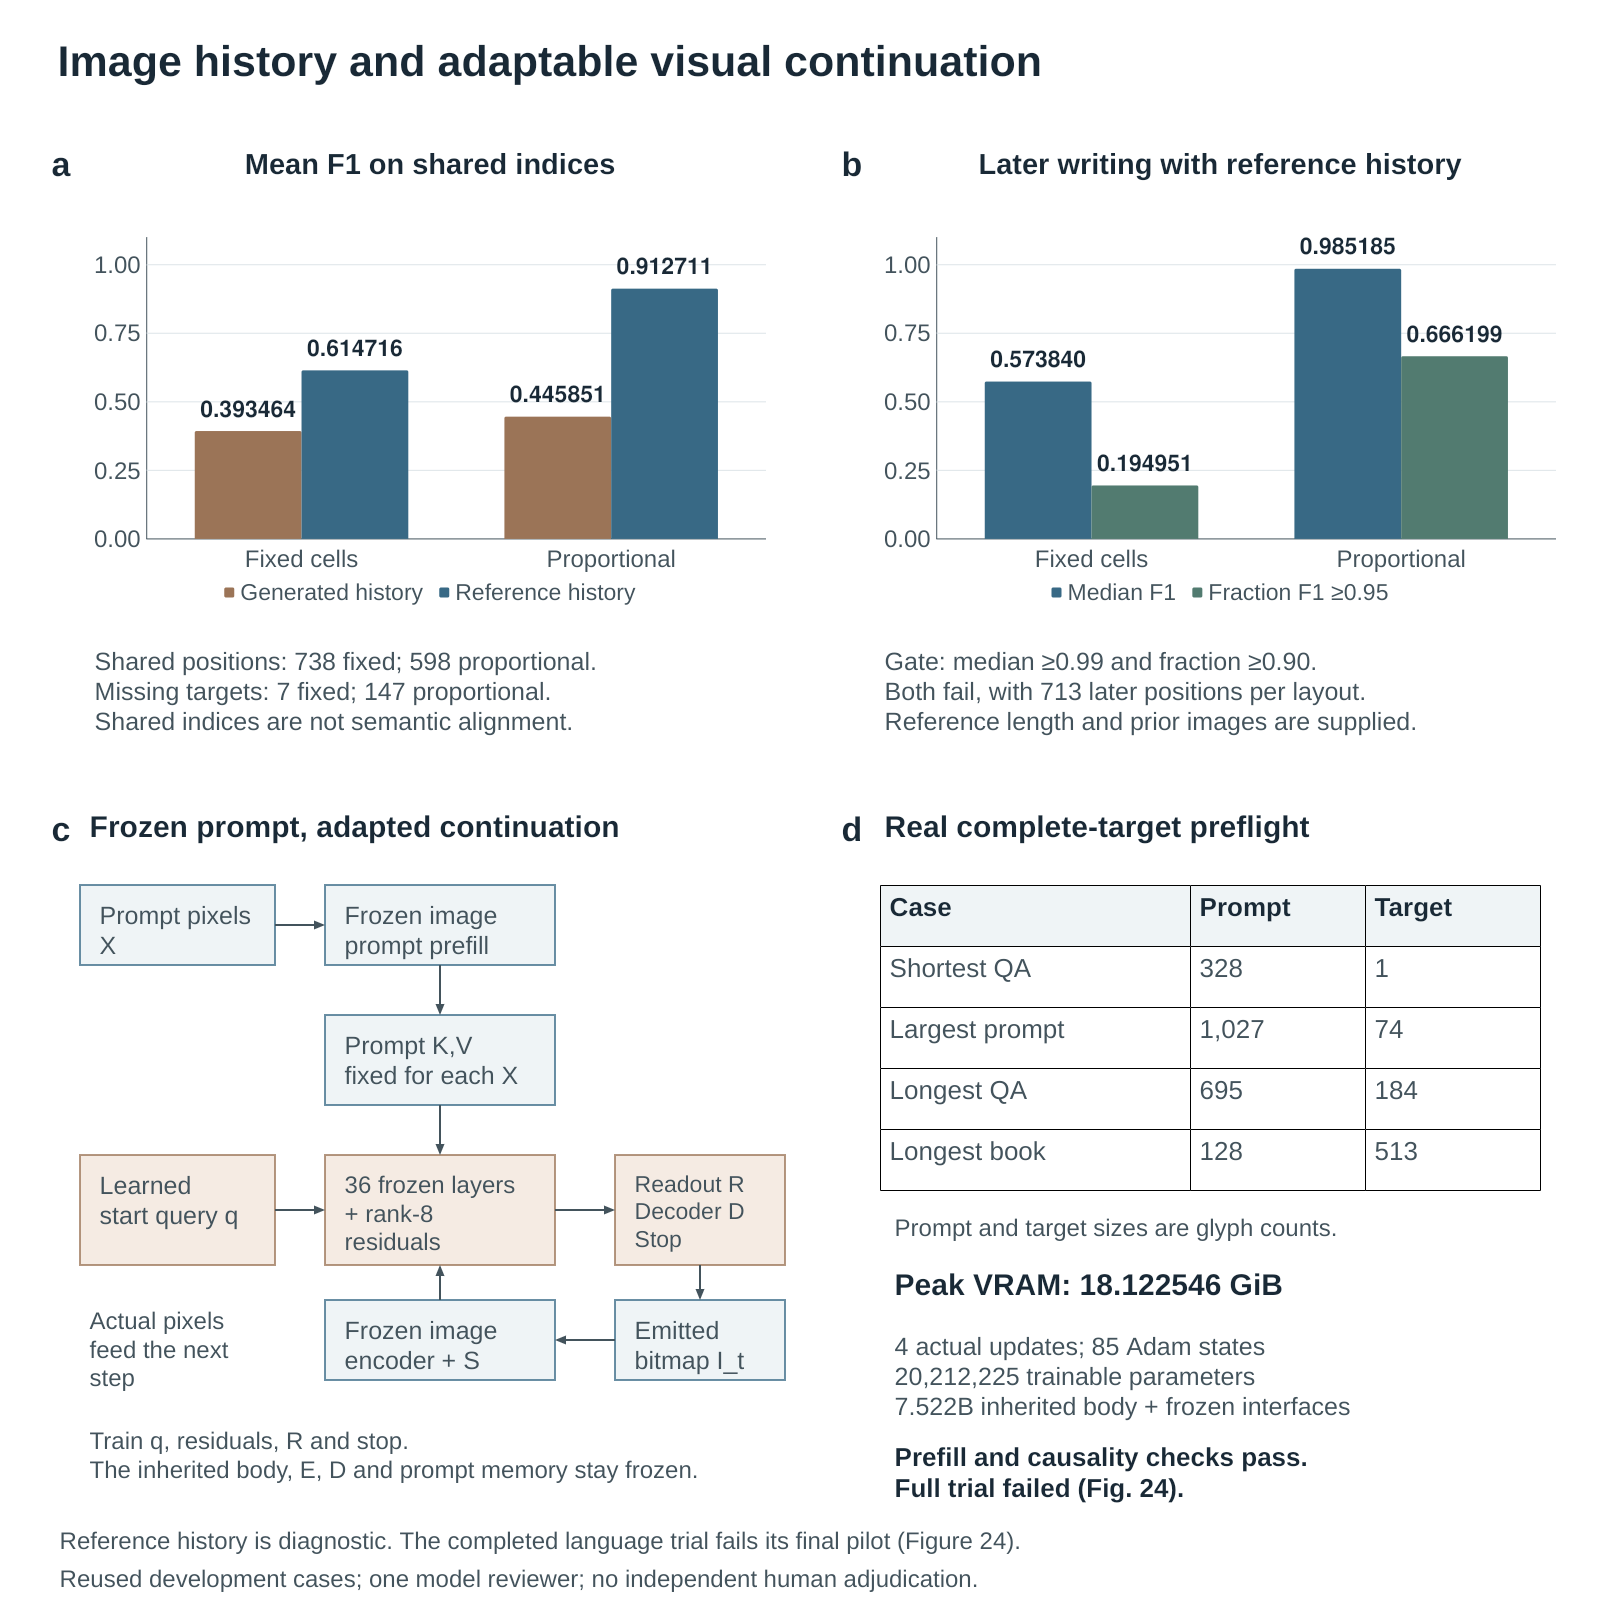
\includegraphics[width=.84\textwidth]{figures/Figure_23_continuation_history_completed.png}
\caption{\DIFaddFL{\textbf{Correct prior images improve canonical writing without qualifying autonomous language.}
\textbf{a}, Mean foreground F1 at target indices present under both generated
and supplied reference-image history: 738 fixed-layout and 598 proportional
positions. Missing and extra autonomous positions remain in the complete
records. Numeric index agreement does not align alternative semantic answers.
Reference history supplies answer information and length, with stopping bypassed.
\textbf{b}, Median later F1 and the fraction of later positions reaching 0.95,
using all 713 later reference positions per layout. Both layouts fail the joint
median/count gate. These canonical image metrics are not language accuracies.
\textbf{c}, Implemented continuation computation. Frozen prompt prefill creates
immutable prompt keys and values. The query and all 36 native answer layers
continue from visible glyph images; new residuals, readout and stopping train,
while the inherited body, image encoder/decoder and affine transform remain
frozen. The stopping head is separate from decoded pixels. Only actually emitted
images supply subsequent inputs; every answer layer is recomputed during fitting.
\textbf{d}, Four complete preflight cases retain all 772 target positions and
four terminal boundaries. Four real optimizer updates peak at 18.122546\,GiB
allocated GPU memory. Independent audits check targets, optimizer states and
numerical boundaries; prompt/frozen-body checks come from the registered GPU
execution. Initial residual-down tensors were not archived in that preflight.
The 7.522B inherited body and frozen interfaces remain deployed costs beyond
the 20,212,225 trainable parameters. F1 chart cells and labels round to six
decimals; complete precision remains in bound records. The supplied-history
diagnosis and preflight are separate from the completed full fit, whose final
language pilot fails (Fig.~24). The later joint writer
has no measured language result here. Reused development data and one model
reviewer with prior familiarity lack independent human adjudication or untouched
confirmation.}}
\label{fig:continuation-history}
\end{figure*}
\begin{figure*}[p]
\centering
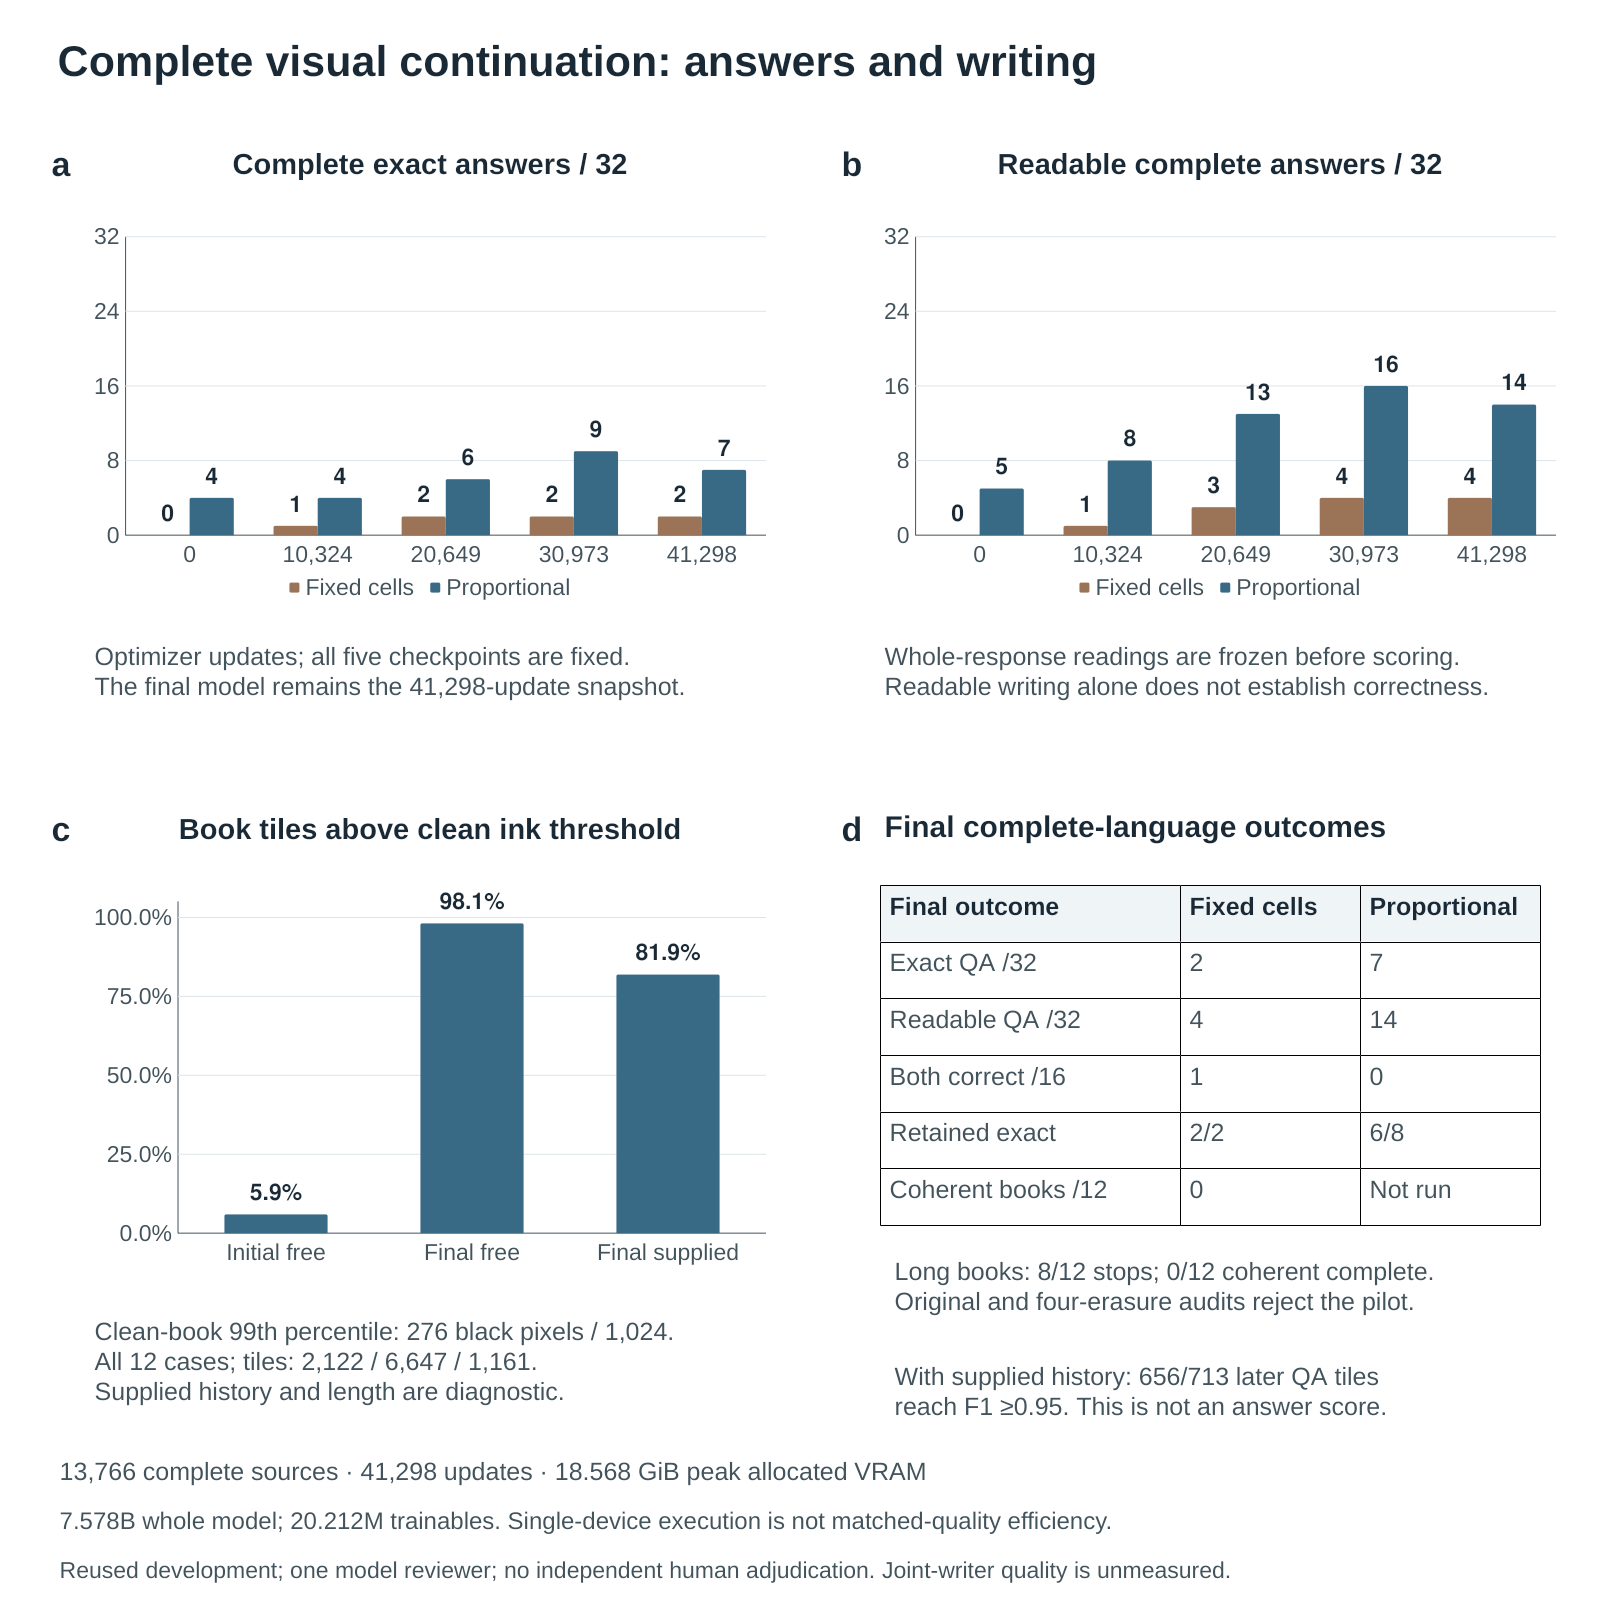
\includegraphics[width=.84\textwidth]{figures/Figure_24_complete_continuation.png}
\caption{\DIFaddFL{\textbf{Complete visual-continuation adaptation improves some short answers
but fails sustained writing.}
\textbf{a,b,} Frozen whole-response exact and readable counts at all five fixed
checkpoints, with 32 questions and sixteen paired passage groups per layout.
The three-quarter peak does not replace the prescribed final model.
\textbf{c,} Fractions of book tiles above the clean training-book 99th-percentile
ink count, 276 of 1,024 pixels. Initial and final autonomous pools contain 2,122
and 6,647 tiles; the final supplied-history pool contains 1,161 target positions.
Each pool retains all twelve prefixes, but lengths differ. Supplied preceding
answer images and length, with stopping bypassed, make the third bar a physical
diagnosis. Chart fractions round to six decimals for workbook storage and percent
labels to one decimal; exact counts and full precision remain in the
source data. Excess ink alone does not establish its cause or a stable attractor.
\textbf{d,} Final complete-answer, paired and retained-success counts. Book prompts
use only the fixed layout; no normal book arm receives a coherent complete
continuation. The 656/713 later QA positions reaching F1 0.95 use supplied history
and do not replace autonomous answer scores. Both the original pilot and the
four-QA-erasure audit reject the final model. The full deployment retains
7.578 billion parameters; one-GPU execution does not establish a matched-quality
efficiency advantage. All results use reused development data and one model
reviewer, with no independent human adjudication. The subsequent joint writer
has no language result in this figure.}}
\label{fig:complete-continuation}
\end{figure*}
\begin{figure*}[p]
\centering
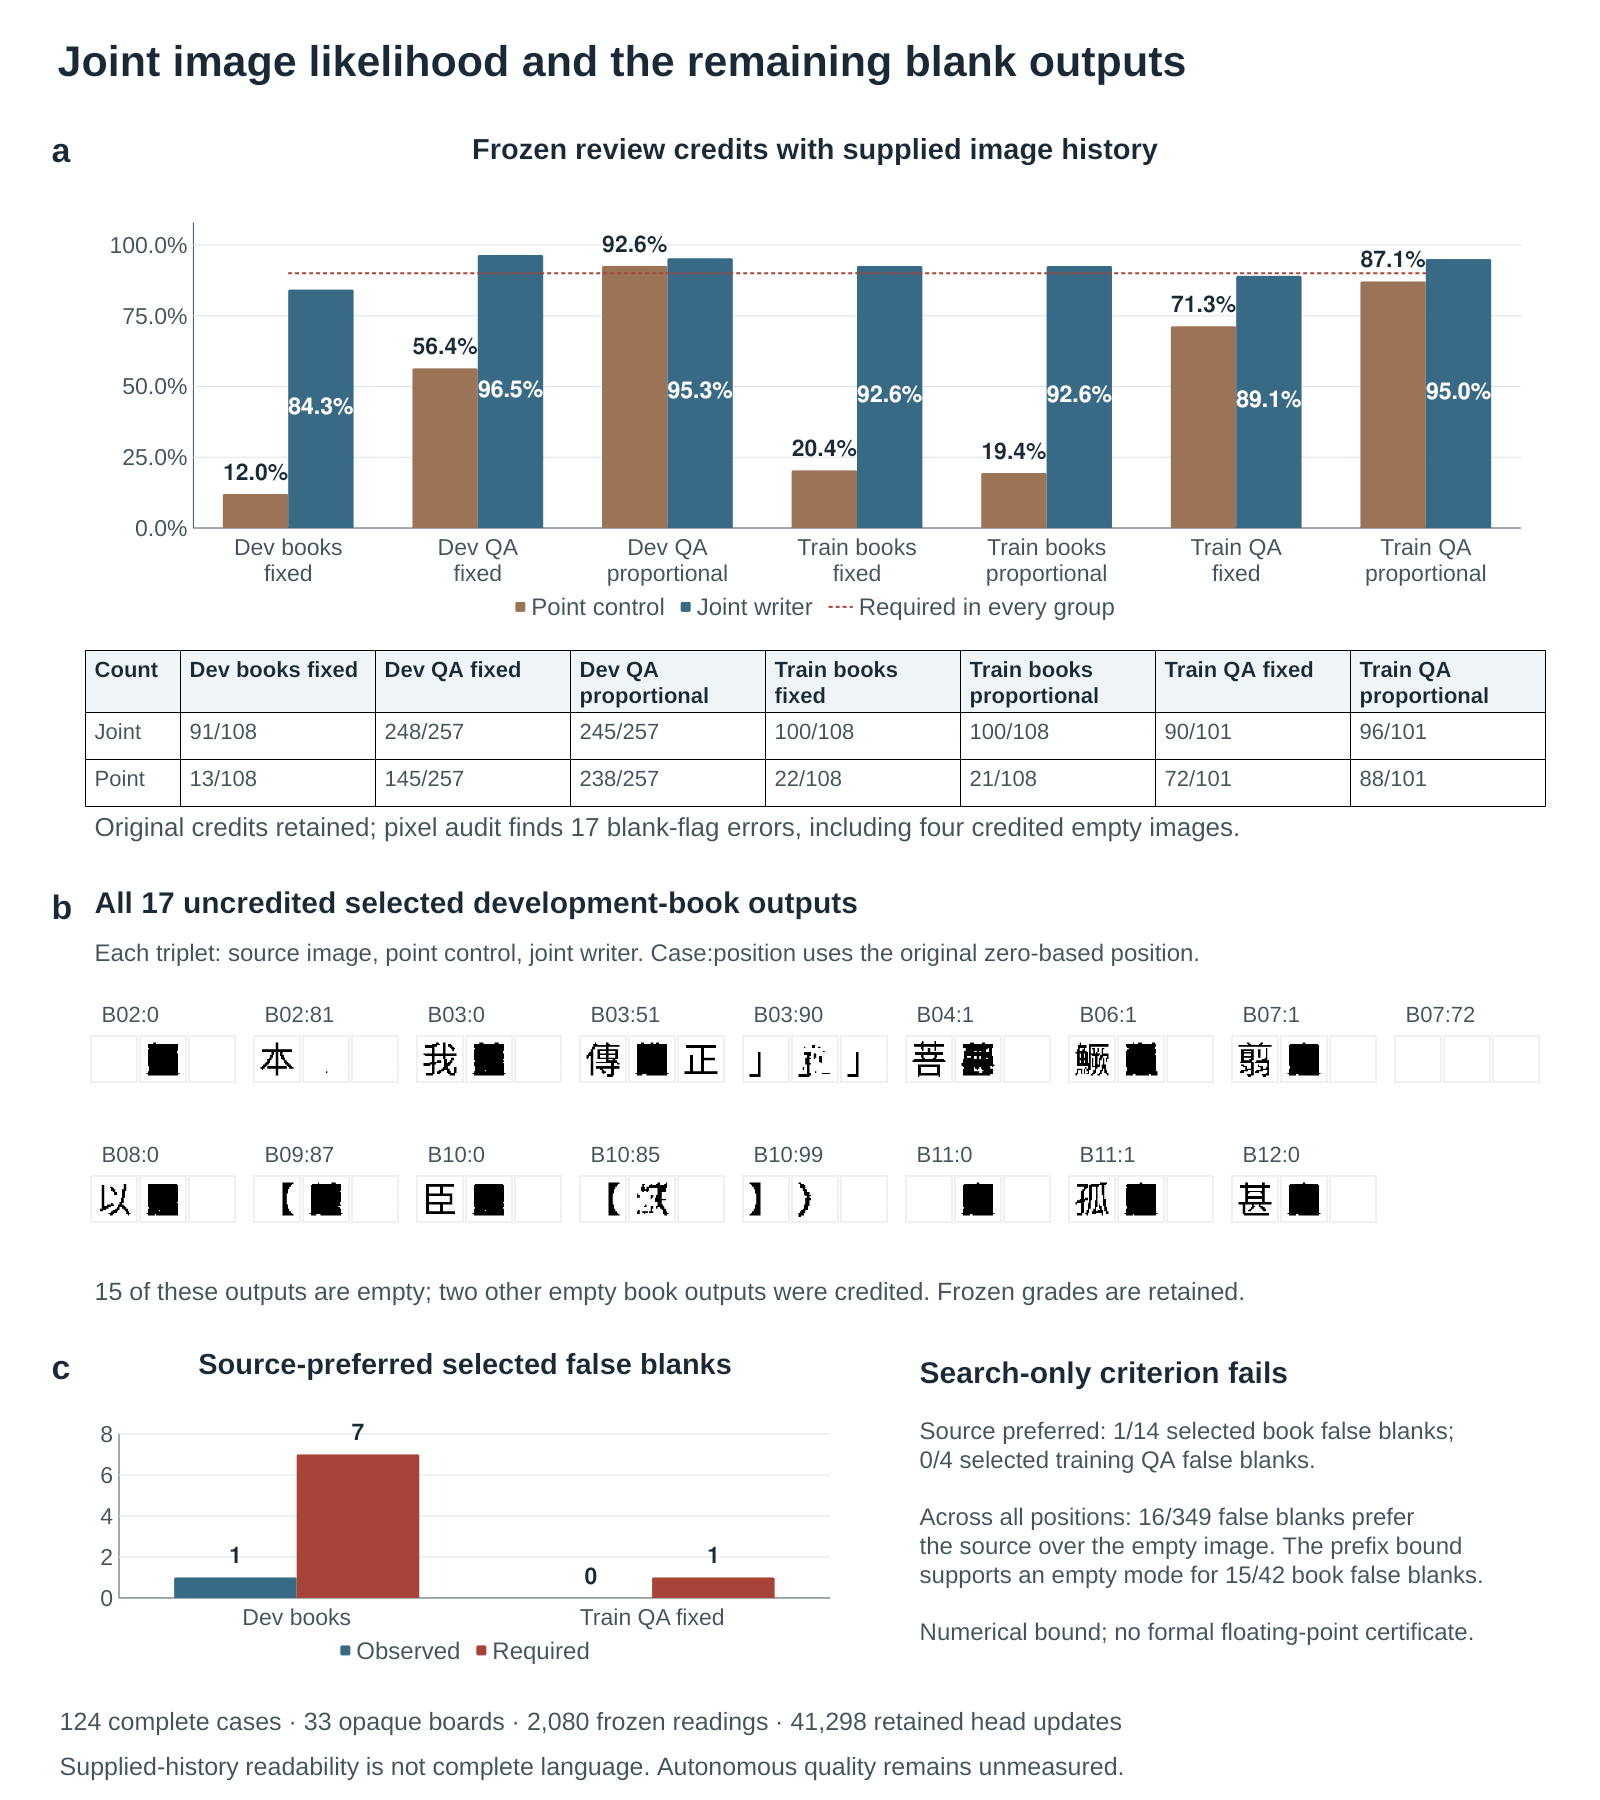
\includegraphics[width=.84\textwidth]{figures/Figure_25_joint_writer_physical.png}
\caption{\DIFaddFL{\textbf{Joint image likelihood changes conditional writing but fails physical qualification.}
\textbf{a,} Original frozen readability credits for the joint writer and unchanged point-writer control in all seven supplied-history groups. The dashed line is the prespecified 90\% prerequisite for every candidate group. Exact counts accompany the chart; chart fractions are rounded to six decimal places. Development books and training QA with fixed cells fail. These are retained review counts, not corrected physical accuracy: a subsequent pixel audit finds 17 blank-flag disagreements among 2,080 readings, including four credited empty images. \textbf{b,} Every uncredited selected development-book output, ordered by case and original zero-based position. Each triplet shows the source, point control and joint output. Original binary $32\times32$ images are expanded threefold by nearest neighbour, without repair. Fifteen of these seventeen joint outputs are empty and two are nonempty; two other empty book outputs were credited. Among all 108 selected book positions, four source images are blank, three overlapping the seventeen empty outputs, giving fourteen false blanks. \textbf{c,} Complete-image likelihood prefers the source over the empty image for one of fourteen selected book false blanks and none of four selected training-QA false blanks, below the unchanged requirements of seven and one. Across all 12,597 positions, sixteen of 349 false blanks prefer their source; the prefix bound supports an empty mode in fifteen of 42 development-book false blanks. The finite-precision bound is not a formal certificate. Review used one model reviewer with prior cohort familiarity and no independent human adjudication. Frozen readings, original scores and the failed verdict are preserved. Autonomous language quality remains unmeasured.}}
\label{fig:joint-writer-physical}
\end{figure*}
\begin{figure*}[p]
\centering
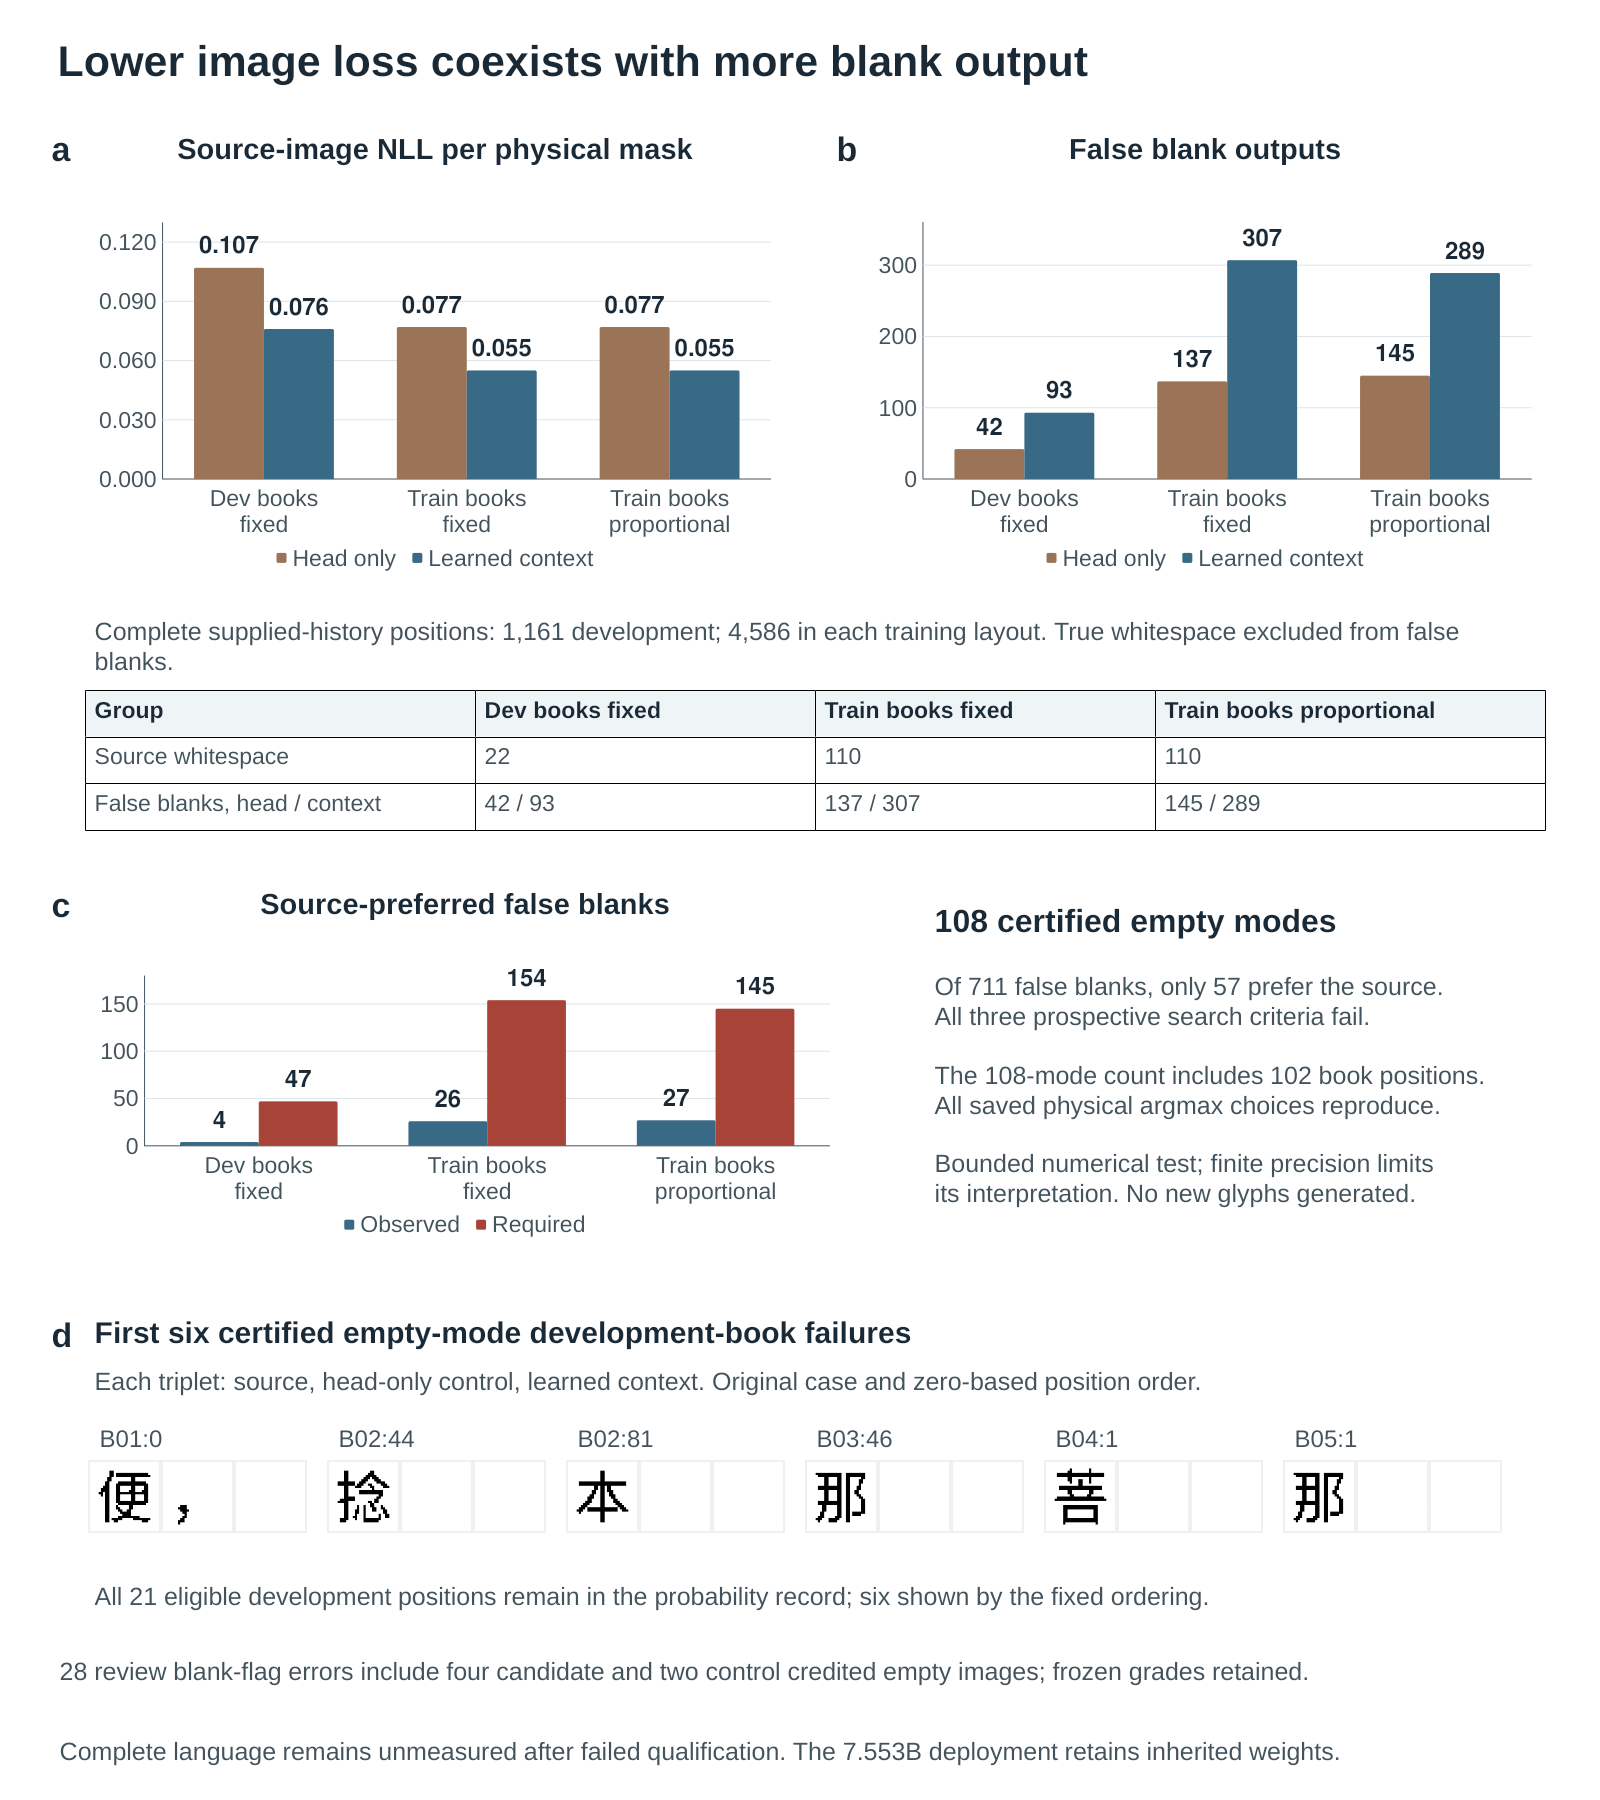
\includegraphics[width=.84\textwidth]{figures/Figure_26_context_likelihood_failure.png}
\caption{\DIFaddFL{\textbf{Lower image likelihood loss does not ensure nonempty conditional writing.}
\textbf{a,b,} Mean source-mask negative log likelihood and false-blank counts
for the same complete supplied-history book groups, comparing the head-only
control with learned continuation context. NLL chart/workbook values round to
three decimals; full precision remains in the bound source data. Counts are
exact. False blanks exclude genuinely empty sources, counted in the table.
Every group retains all positions; development has 1,161 and each training
layout 4,586. \textbf{c,} Complete-image source preference among false blanks,
using the fixed 0.001-nat margin. The observed counts 4/93, 26/307 and 27/289
miss the prospective minimum counts 47, 154 and 145. Across all seven groups,
57/711 false blanks prefer the source; the zero-prefix upper bound supports
an empty global mode at 108 false blanks, including 102 book positions.
The numerical inequality is subject to finite precision and is not a formal
certificate. All saved physical argmax choices reproduce.
\textbf{d,} The first six of 21 development-book certified empty-mode failures,
ordered by original case and zero-based position. Each triplet retains source,
head-only and learned-context binary pixels, expanded threefold by nearest
neighbour without repair. All source samples contain ink and all shown context
outputs are empty. The complete probability record retains all eligible cases.
Original review grades remain frozen despite 28 contradictory blank flags,
including four candidate and two control credited empty images. One model
reviewer had prior cohort familiarity; independent human adjudication is absent.
The failed physical prerequisite prevents autonomous evaluation. Neither lower
likelihood loss nor this diagnostic establishes complete language, a compact
foundation or matched-quality efficiency.}}
\label{fig:context-likelihood-failure}
\end{figure*}
\begin{figure*}[p]
\centering
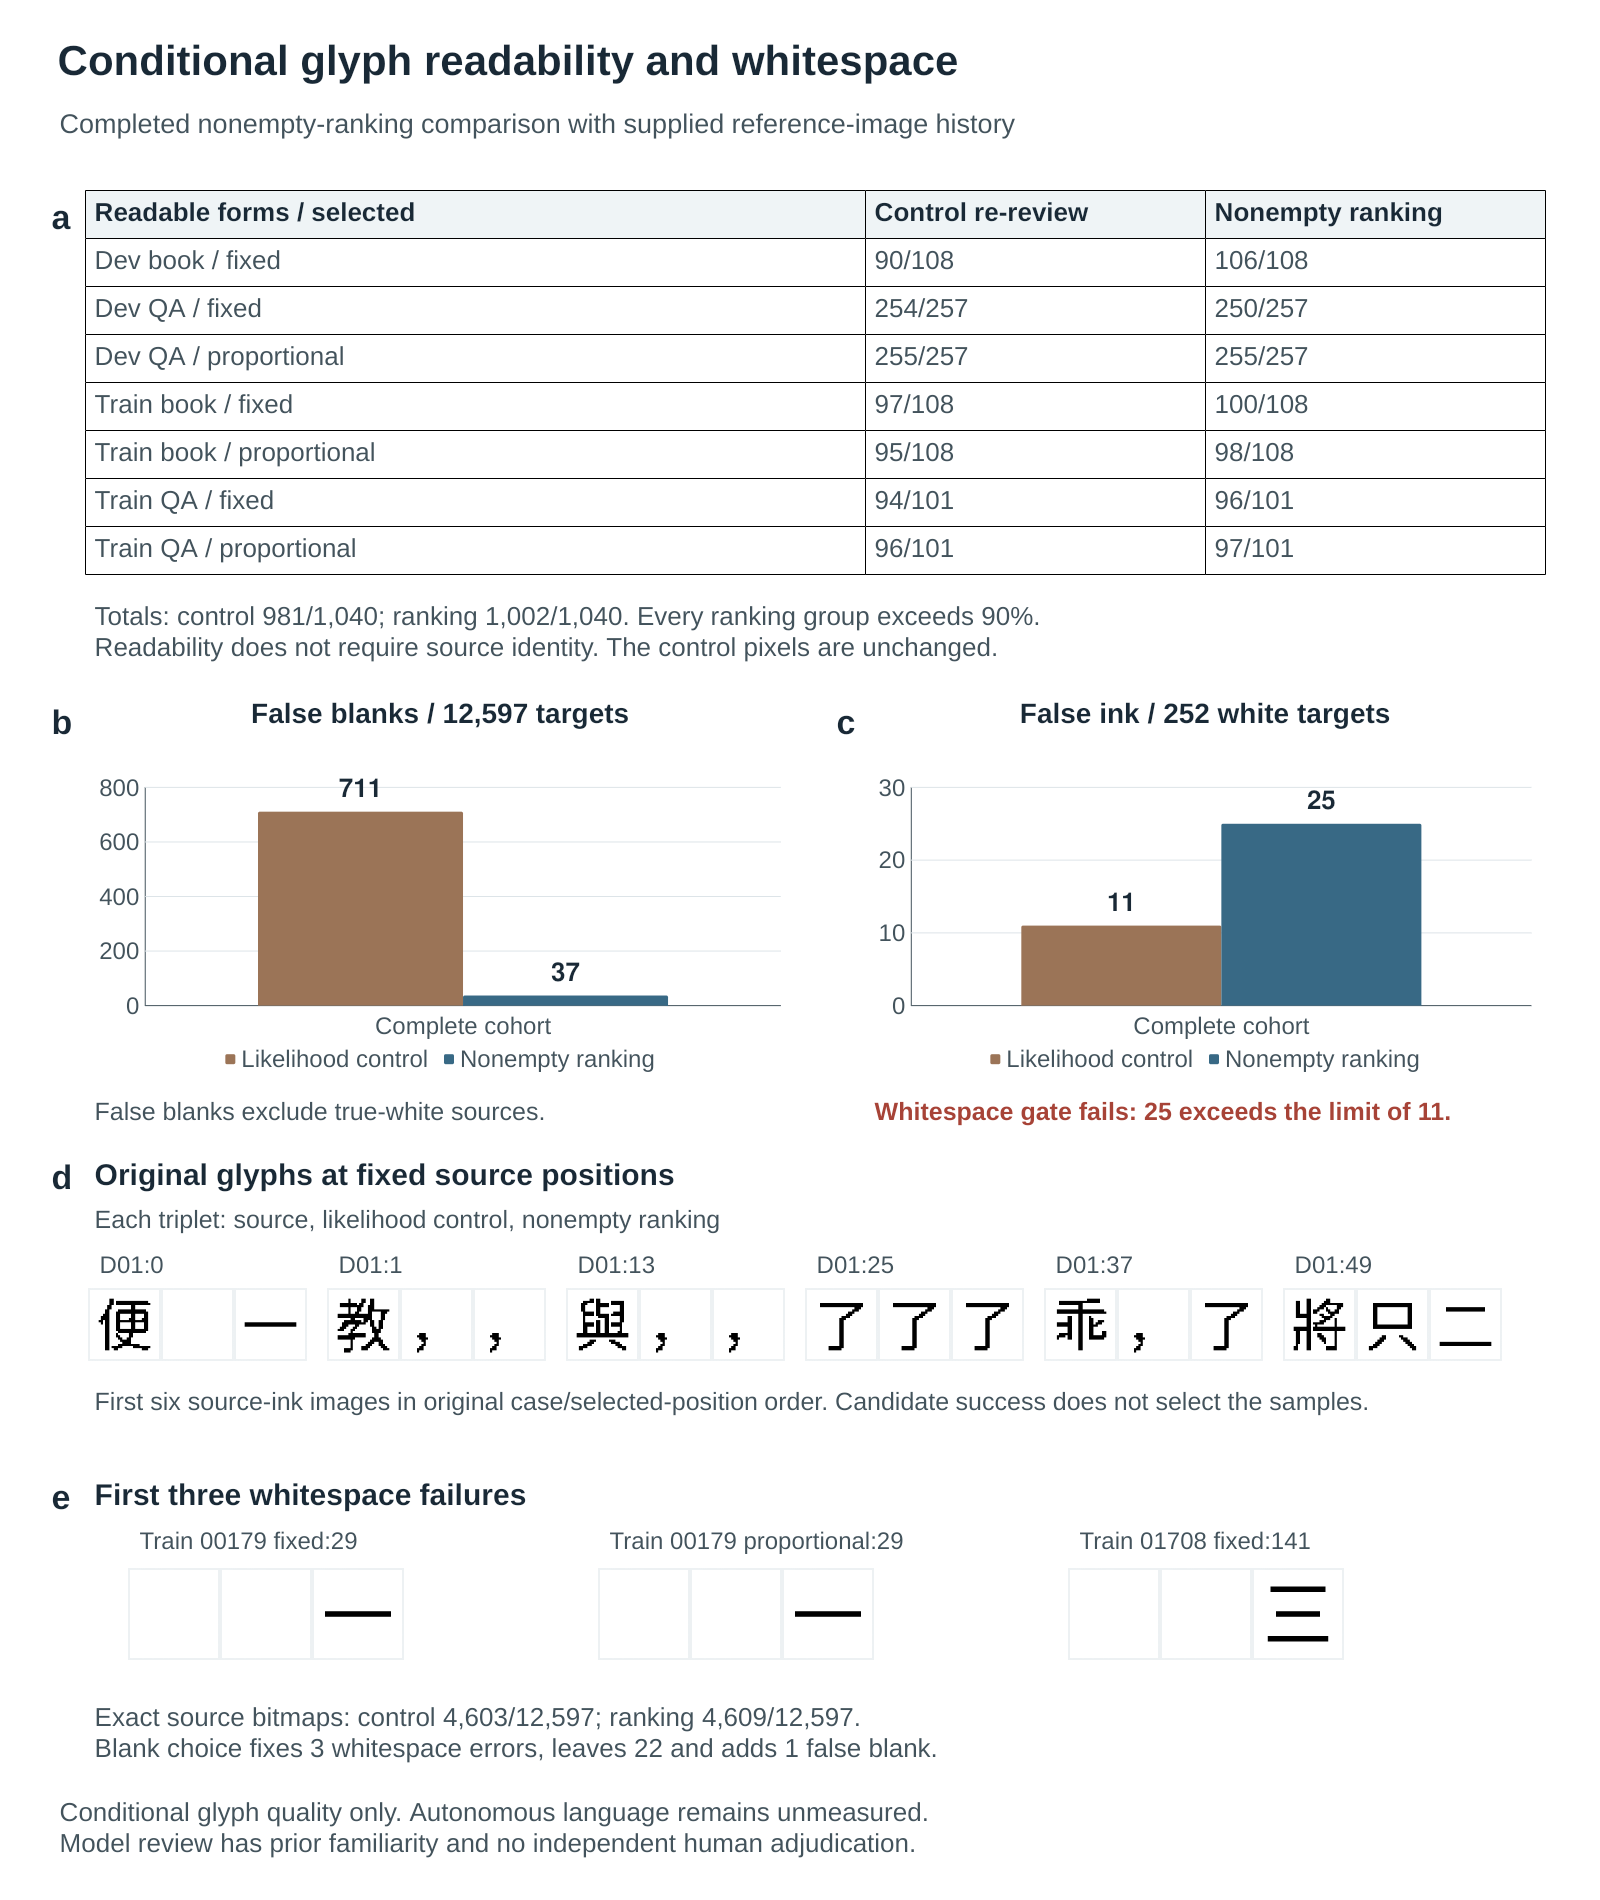
\includegraphics[width=.84\textwidth]{figures/Figure_27_ranking_completed.png}
\caption{\DIFaddFL{\textbf{Fewer blank images do not establish correct writing.}
\textbf{a,} All seven original readable-form groups from the completed
nonempty-ranking comparison. A credit requires recognizable nonempty writing
without uncertainty, not source identity or correct meaning. The control
pixels are unchanged; their fresh 981/1,040 review credits do not replace the
original frozen 970/1,040. \textbf{b,c,} Complete-array false blanks decrease
from 711 to 37, but false ink increases from eleven to twenty-five among 252
genuinely white source images, failing the prospective maximum of eleven.
Exact source bitmaps change only from 4,603 to 4,609 of 12,597 positions.
\textbf{d,} The first six source-ink images in original development-book
case/selected-position order, without selecting candidate success. D01 denotes
the first development book; positions are zero-based. Each triplet retains
source, likelihood-control and ranked-output pixels. \textbf{e,} The first
three false-ink source-white failures in complete-case/position order.
Binary 32-by-32 pixels are expanded threefold by nearest neighbour without
repair. The complete-density blank choice would fix three spaces, leave
twenty-two and erase one additional nonempty position; no output or gate changes.
All cases use supplied reference-image history. One model reviewer has prior
familiarity and no independent human adjudication; initial unfrozen entry
corrections were preserved before the sole freeze. All current blank flags
agree with pixels, but older review errors remain unchanged. Complete language
and the separate blank-target fit's quality remain unmeasured.}}
\label{fig:ranking-completed}
\end{figure*}
\begin{figure*}[p]
\centering
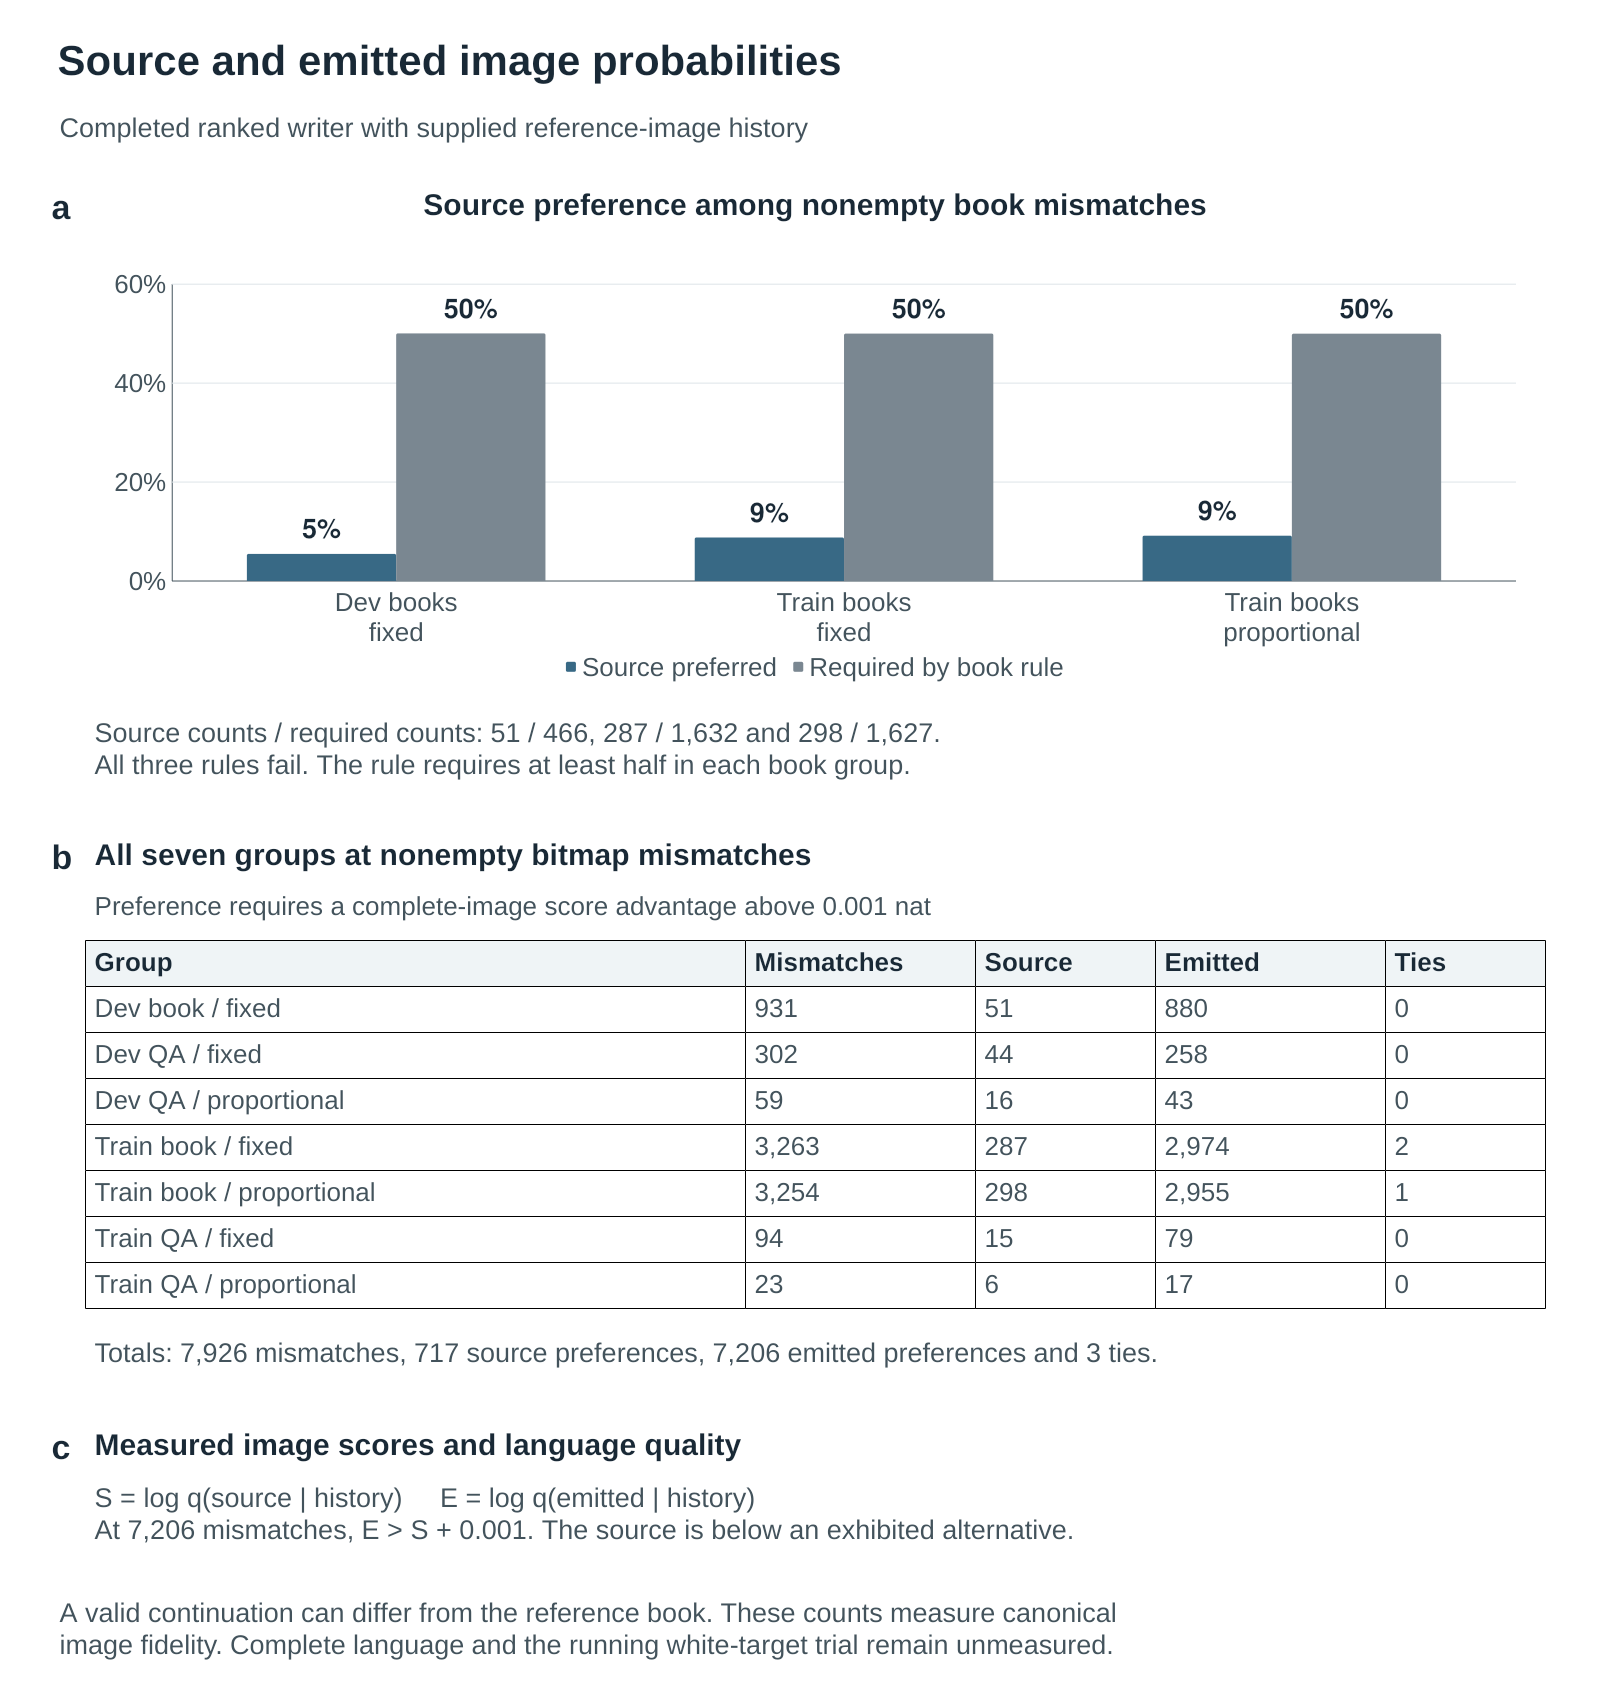
\includegraphics[width=.84\textwidth]{figures/Figure_28_glyph_score_gaps.png}
\caption{\DIFaddFL{\textbf{Saved probabilities favor the emitted alternative at most nonempty bitmap mismatches.}
\textbf{a,} Observed source-preference fractions and fixed required fractions in
the three book strata. The requirement is at least half of nonempty mismatches,
rounded upward, separately in every stratum. Chart values round to six decimals
and displayed percentages to whole percentages; exact counts remain in the
table and source data. All three rules fail. \textbf{b,} All seven groups retain
their mismatch denominators and source/emitted/tie counts. A preference requires
a complete-image log-score advantage above 0.001 nat. The counts sum to 717
source preferences, 7,206 emitted preferences and three ties over 7,926 nonempty
bitmap mismatches. \textbf{c,} An exhibited image above the source excludes the
source from the highest measured score. It does not prove the emitted image
globally optimal or measure prefix logits. A valid continuation can differ from
the reference book. All 124 cases and 12,597 supplied-history positions remain;
exact bitmaps, false blanks and false ink are separate categories. The independent
scalar recount agrees without a model call or new output image. This reused-cohort
calculation measures canonical image fidelity rather than semantic accuracy.
At this analysis time the separate white-target trial's quality was unmeasured;
its subsequent physical failure is reported in Fig.~\ref{fig:white-target-completed}.
Autonomous language remains unmeasured for that failed actor.}}
\label{fig:glyph-score-gaps}
\end{figure*}
\begin{figure*}[p]
\centering
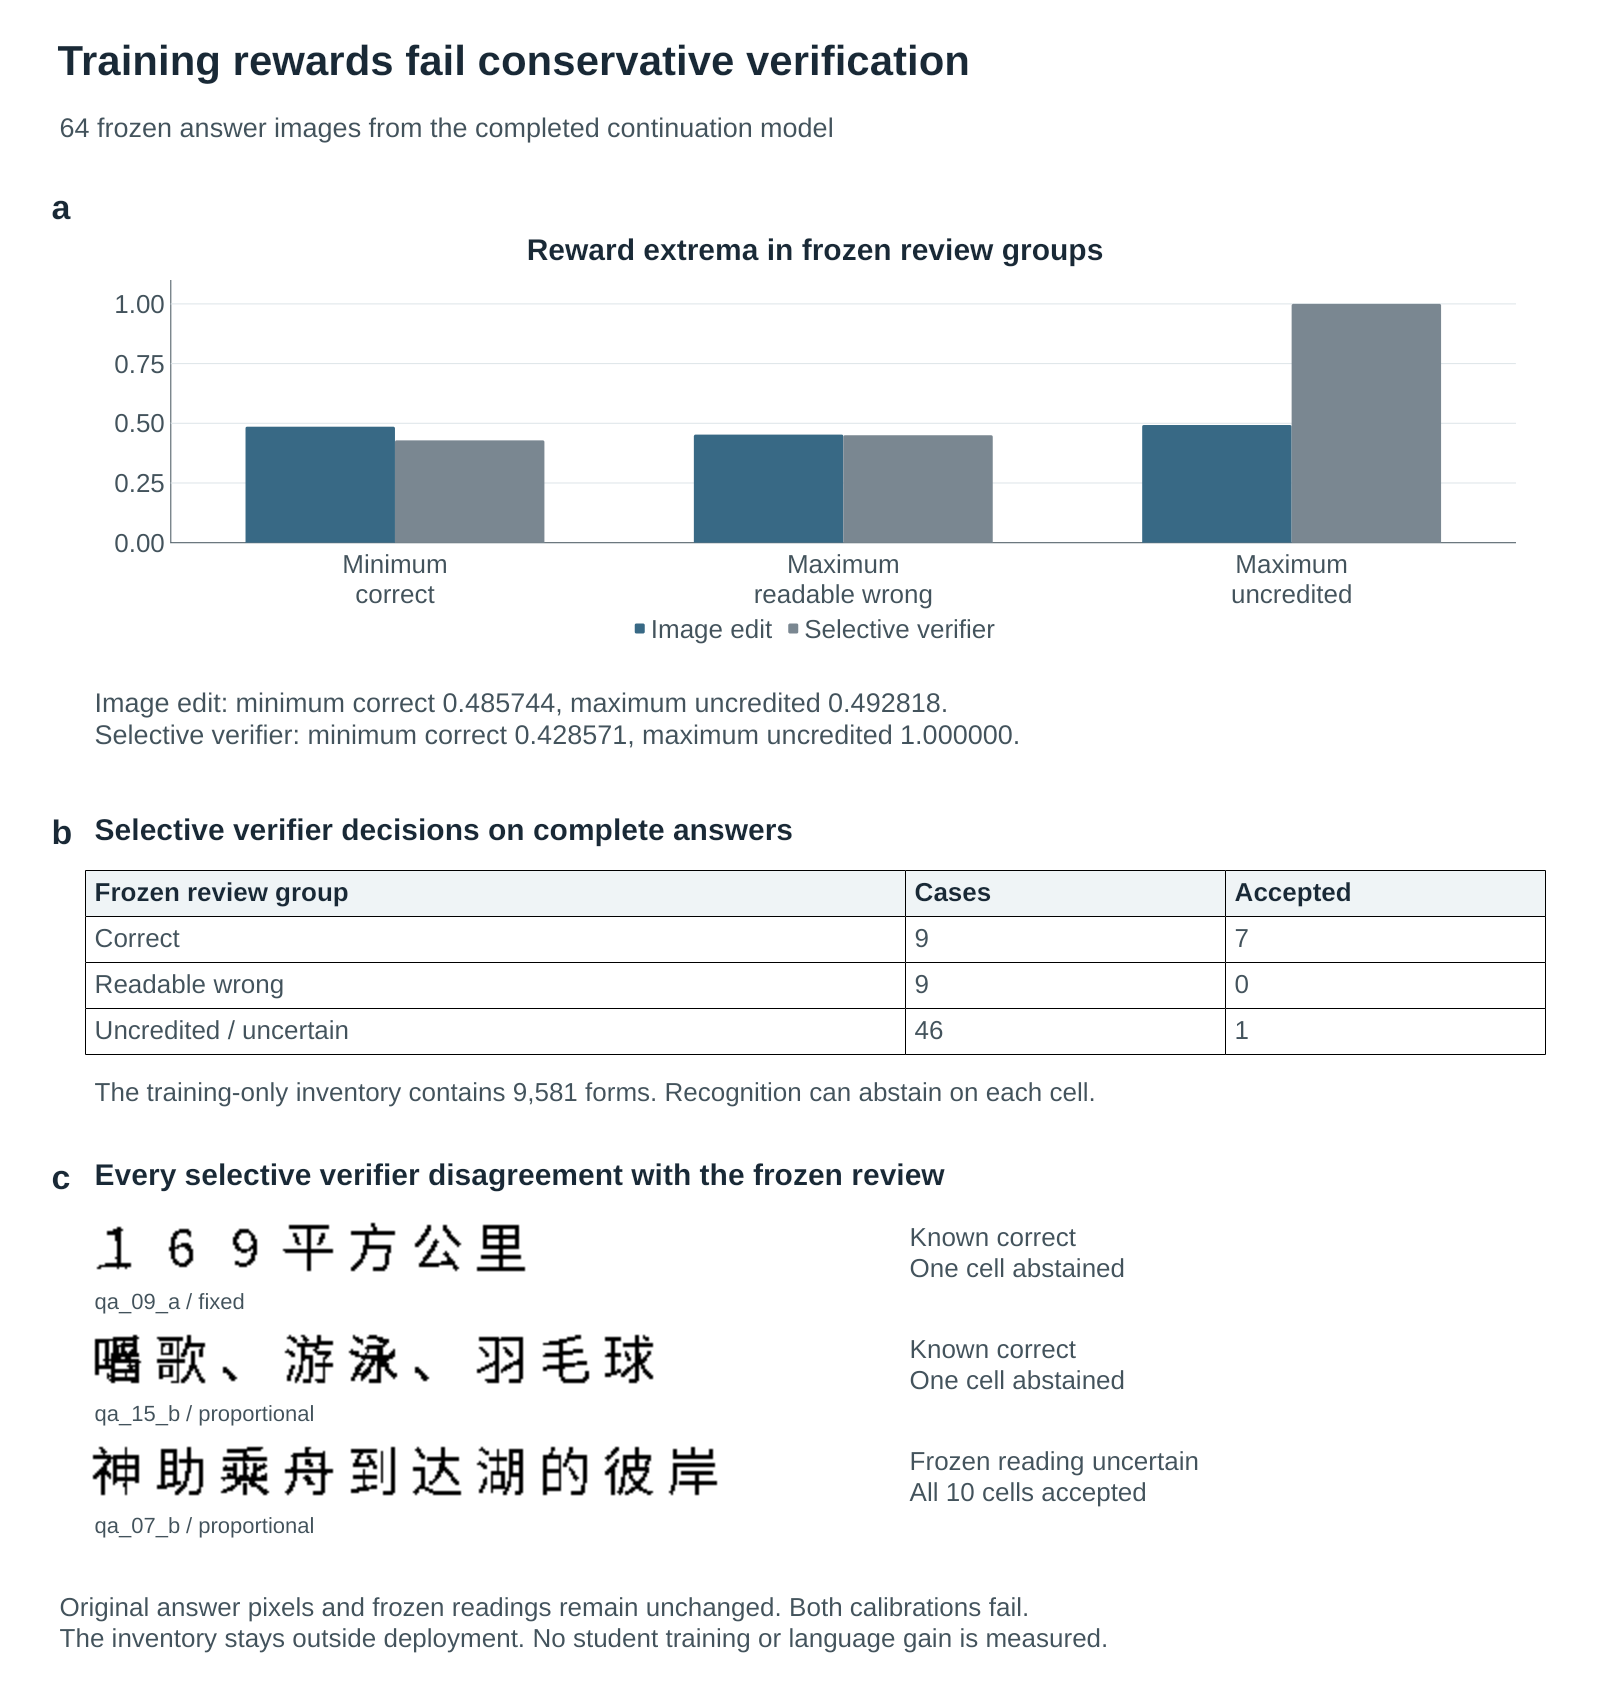
\includegraphics[width=.84\textwidth]{figures/Figure_29_reward_calibration.png}
\caption{\DIFaddFL{\textbf{Two proposed training rewards fail conservative verification on complete image answers.}
\textbf{a,} Minimum strict complete-correct and maximum other-group rewards
across all 64 final normal QA images: 32 questions in two presentations, with
nine correct, nine readable strict mismatches and 46 uncredited or uncertain
outcomes. Values round to six decimals in the native chart workbook. Both
candidates give an uncredited output a reward exceeding their minimum correct
reward. Known-readable AUC values, 1.0 and 0.975309, describe only the 18
known-readable outcomes and do not qualify either reward. \textbf{b,} Every
selective complete-content acceptance count. The finite 9,581-image inventory
uses training pixels only and remains absent from student deployment.
\textbf{c,} Every disagreement under the fixed rule: all known-correct answers
not fully accepted and all uncredited answers fully accepted. The original
answer PNGs are embedded unchanged, with no reference prototype or inferred
replacement transcription. Two correct answers each have one abstained cell;
the uncertain answer has all ten accepted. Its frozen reading remains uncertain.
This disagreement does not establish semantic error or authorize repairing
earlier readings. Both prospective calibrations fail. There is no independent
human adjudication, new model call, optimizer update or measured language gain.}}
\label{fig:reward-calibration}
\end{figure*}
\begin{figure*}[p]
\centering
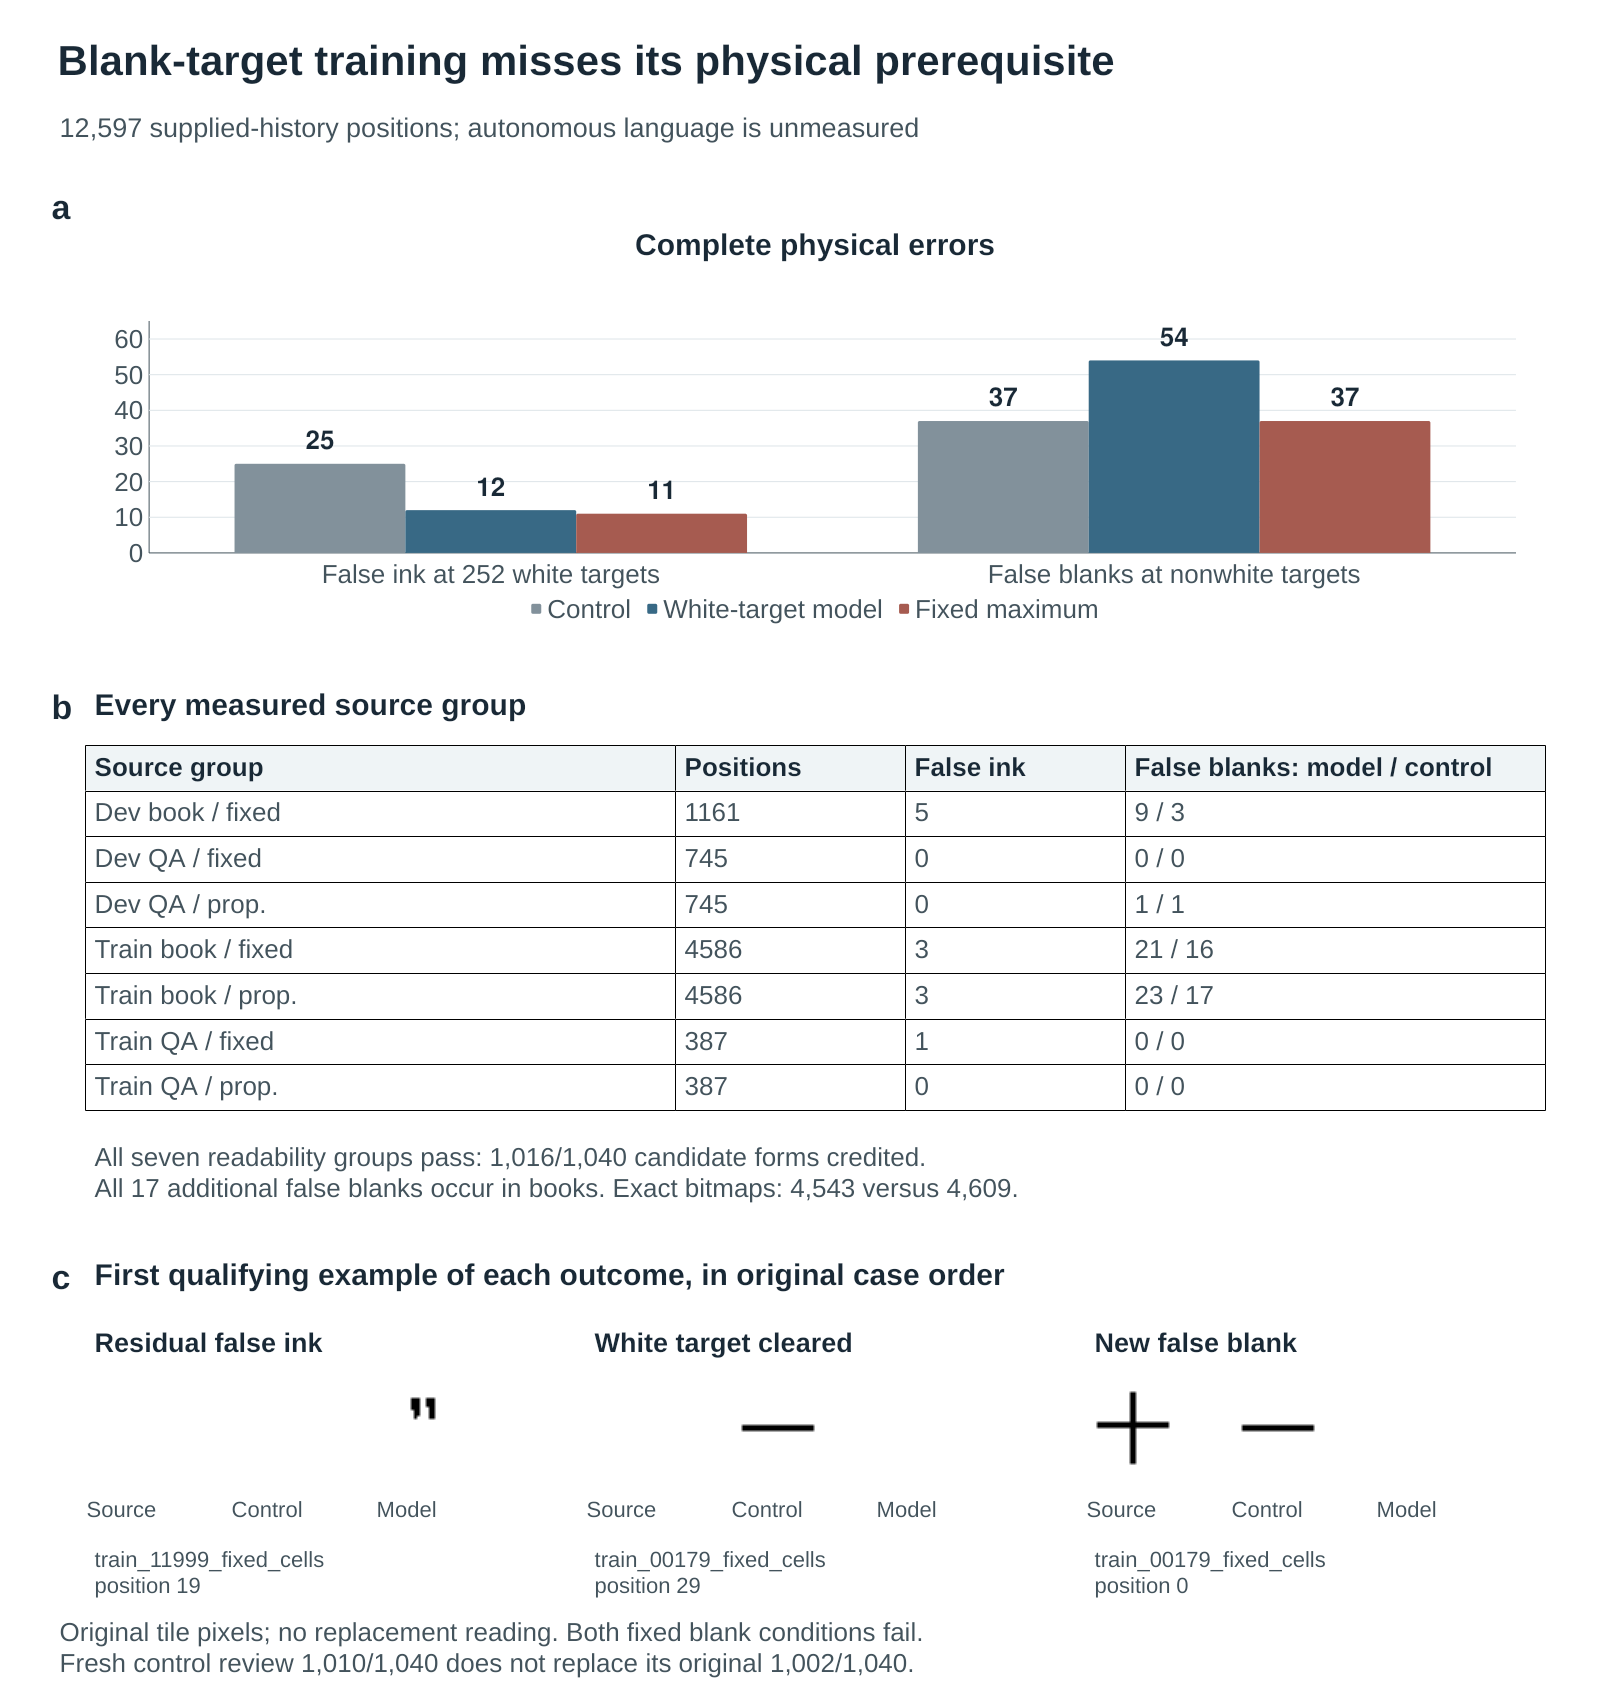
\includegraphics[width=.84\textwidth]{figures/Figure_30_white_target_completed.png}
\caption{\DIFaddFL{\textbf{Blank-target ranking reduces false ink while increasing false blanks.}
\textbf{a,} Complete counts over 12,597 supplied-history positions for the
unchanged control and final white-target model. Fixed maxima are eleven false
ink outputs among 252 true-white positions and 37 false blanks. Candidate counts
12 and 54 fail both conditions. \textbf{b,} Every source group's position and
error counts. All seventeen additional false blanks occur in books. Readable
form credits do not require the source character or a complete correct answer.
Fresh control review 1,010/1,040 does not replace its original 1,002/1,040.
\textbf{c,} Original source/control/candidate tiles for the first occurrence of
each fixed outcome rule in qualification order: residual false ink, a cleared
white target and a newly introduced false blank. No tile or reading is repaired.
These are conditional physical predictions, not autonomous answer excerpts.
The actor fails qualification and its separate language comparison is not run.}}
\label{fig:white-target-completed}
\end{figure*}
\begin{figure*}[p]
\centering
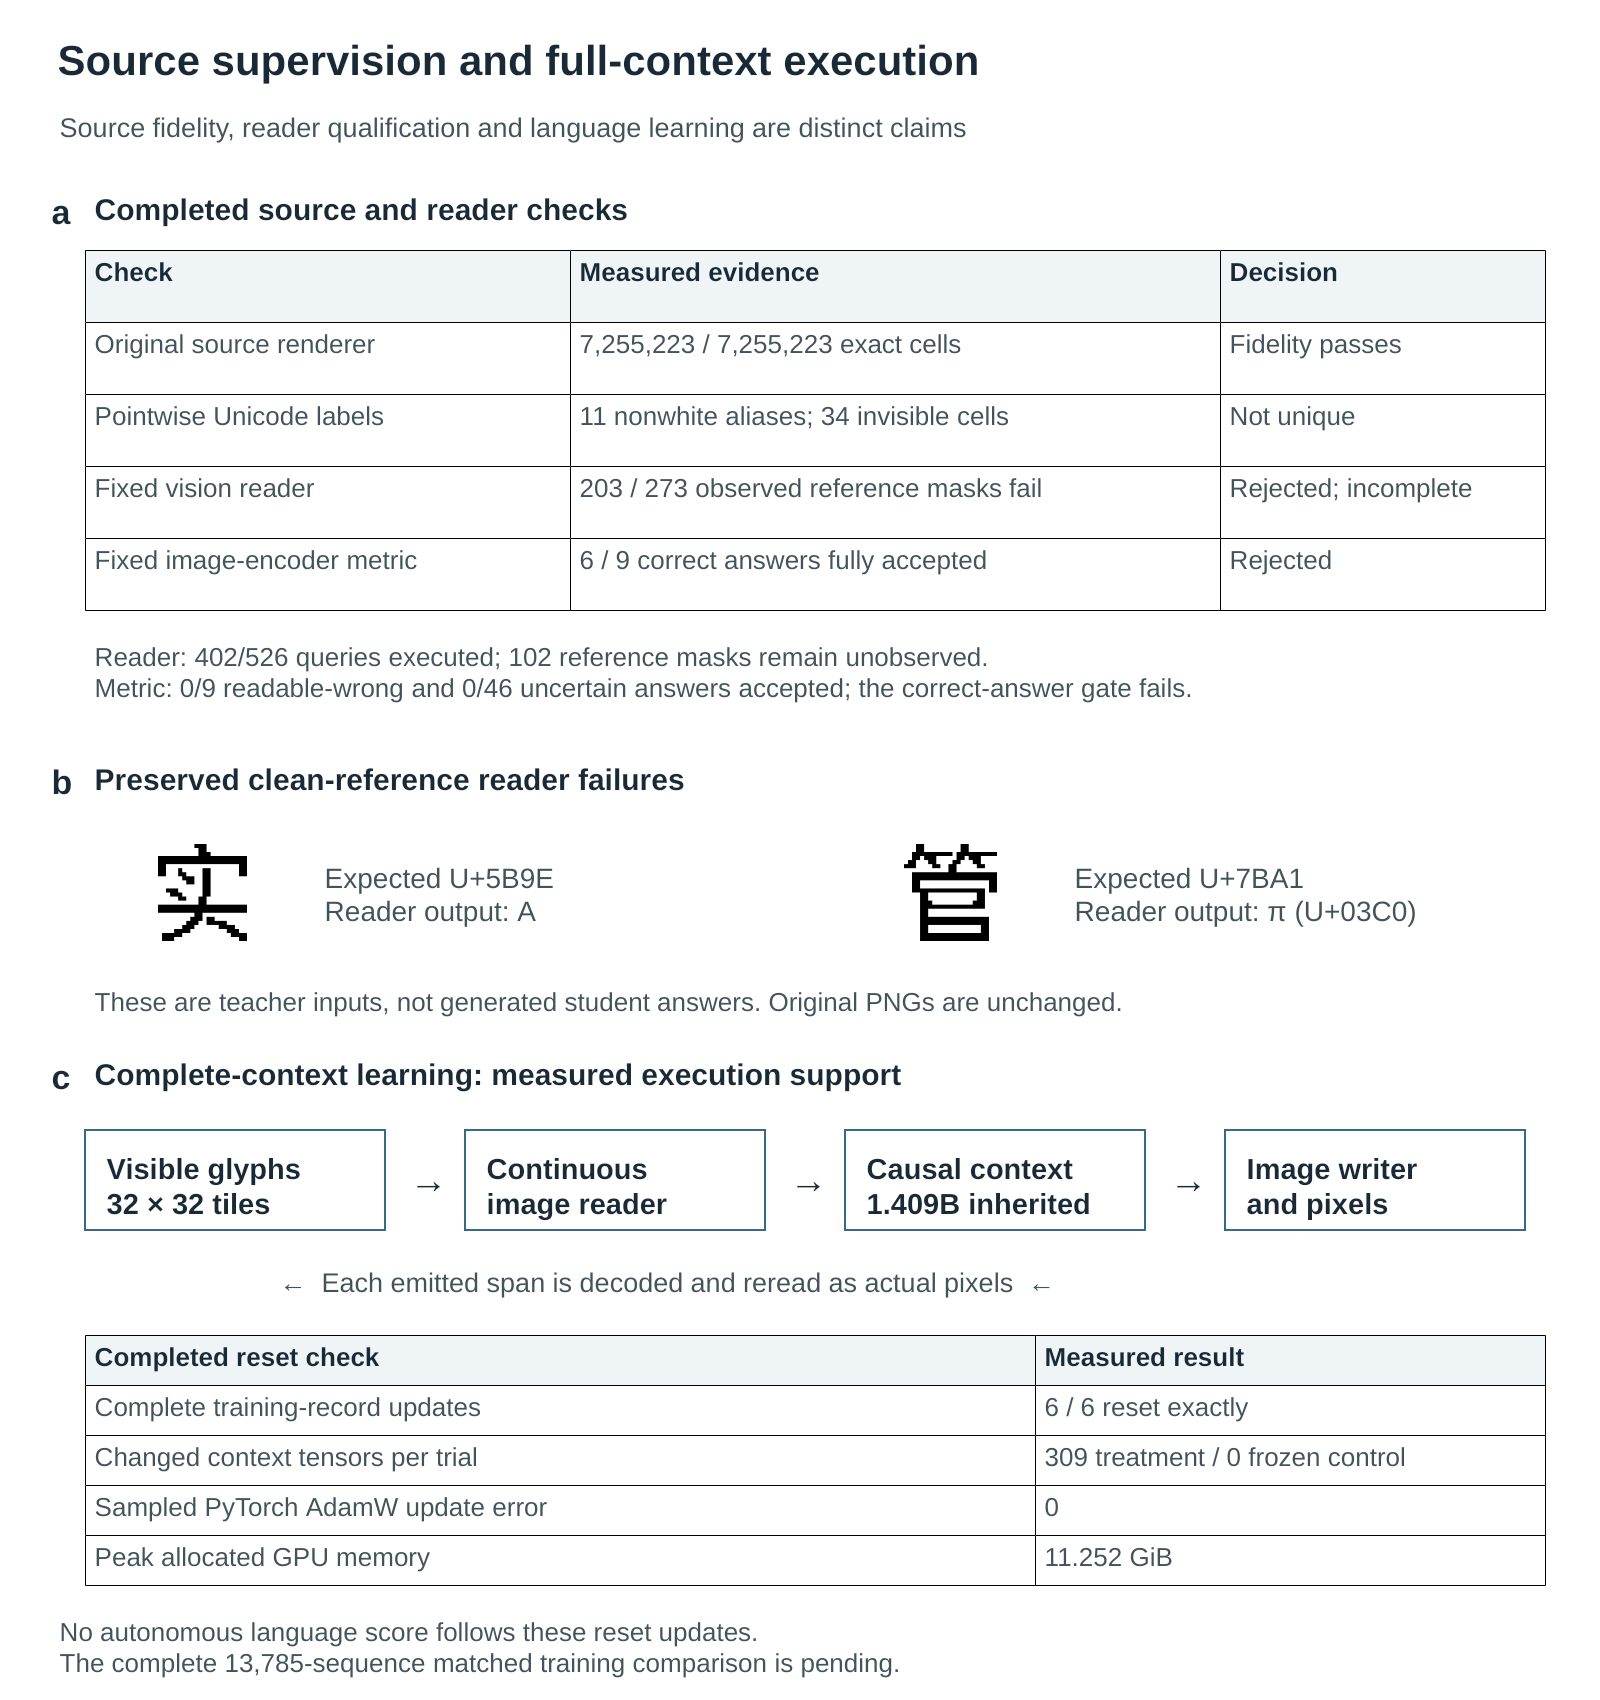
\includegraphics[width=.84\textwidth]{figures/Figure_31_visual_context_evidence.png}
\caption{\DIFaddFL{\textbf{Source fidelity, reader qualification and context learning require separate evidence.}
\textbf{a,} Complete source rendering passes, while isolated Unicode identity
is ambiguous and both fixed reader candidates fail their own prerequisites.
The general vision reader is rejected from observed necessary-condition
failures; 124 queries, including 102 reference masks, remain unexecuted.
\textbf{b,} The first two distinct preserved clean-reference failures, without
image replacement. These are teacher inputs, not student answers.
\textbf{c,} Native editable diagram of the complete-context comparison and
measured support from all six real update/reset trials. Every one of 309 context
tensors changes only in treatment; sampled AdamW update error is zero and all
states reset exactly. The 11.252\,GiB peak is an execution measurement, not a
language score. Figure~\ref{fig:full-context-comparison} reports the subsequent trained outputs.
Inherited text pretraining remains a source of knowledge; neither independent
from-scratch vision-language learning nor matched-quality efficiency is proved.}}
\label{fig:visual-context-evidence}
\end{figure*}
\begin{figure*}[p]
\centering
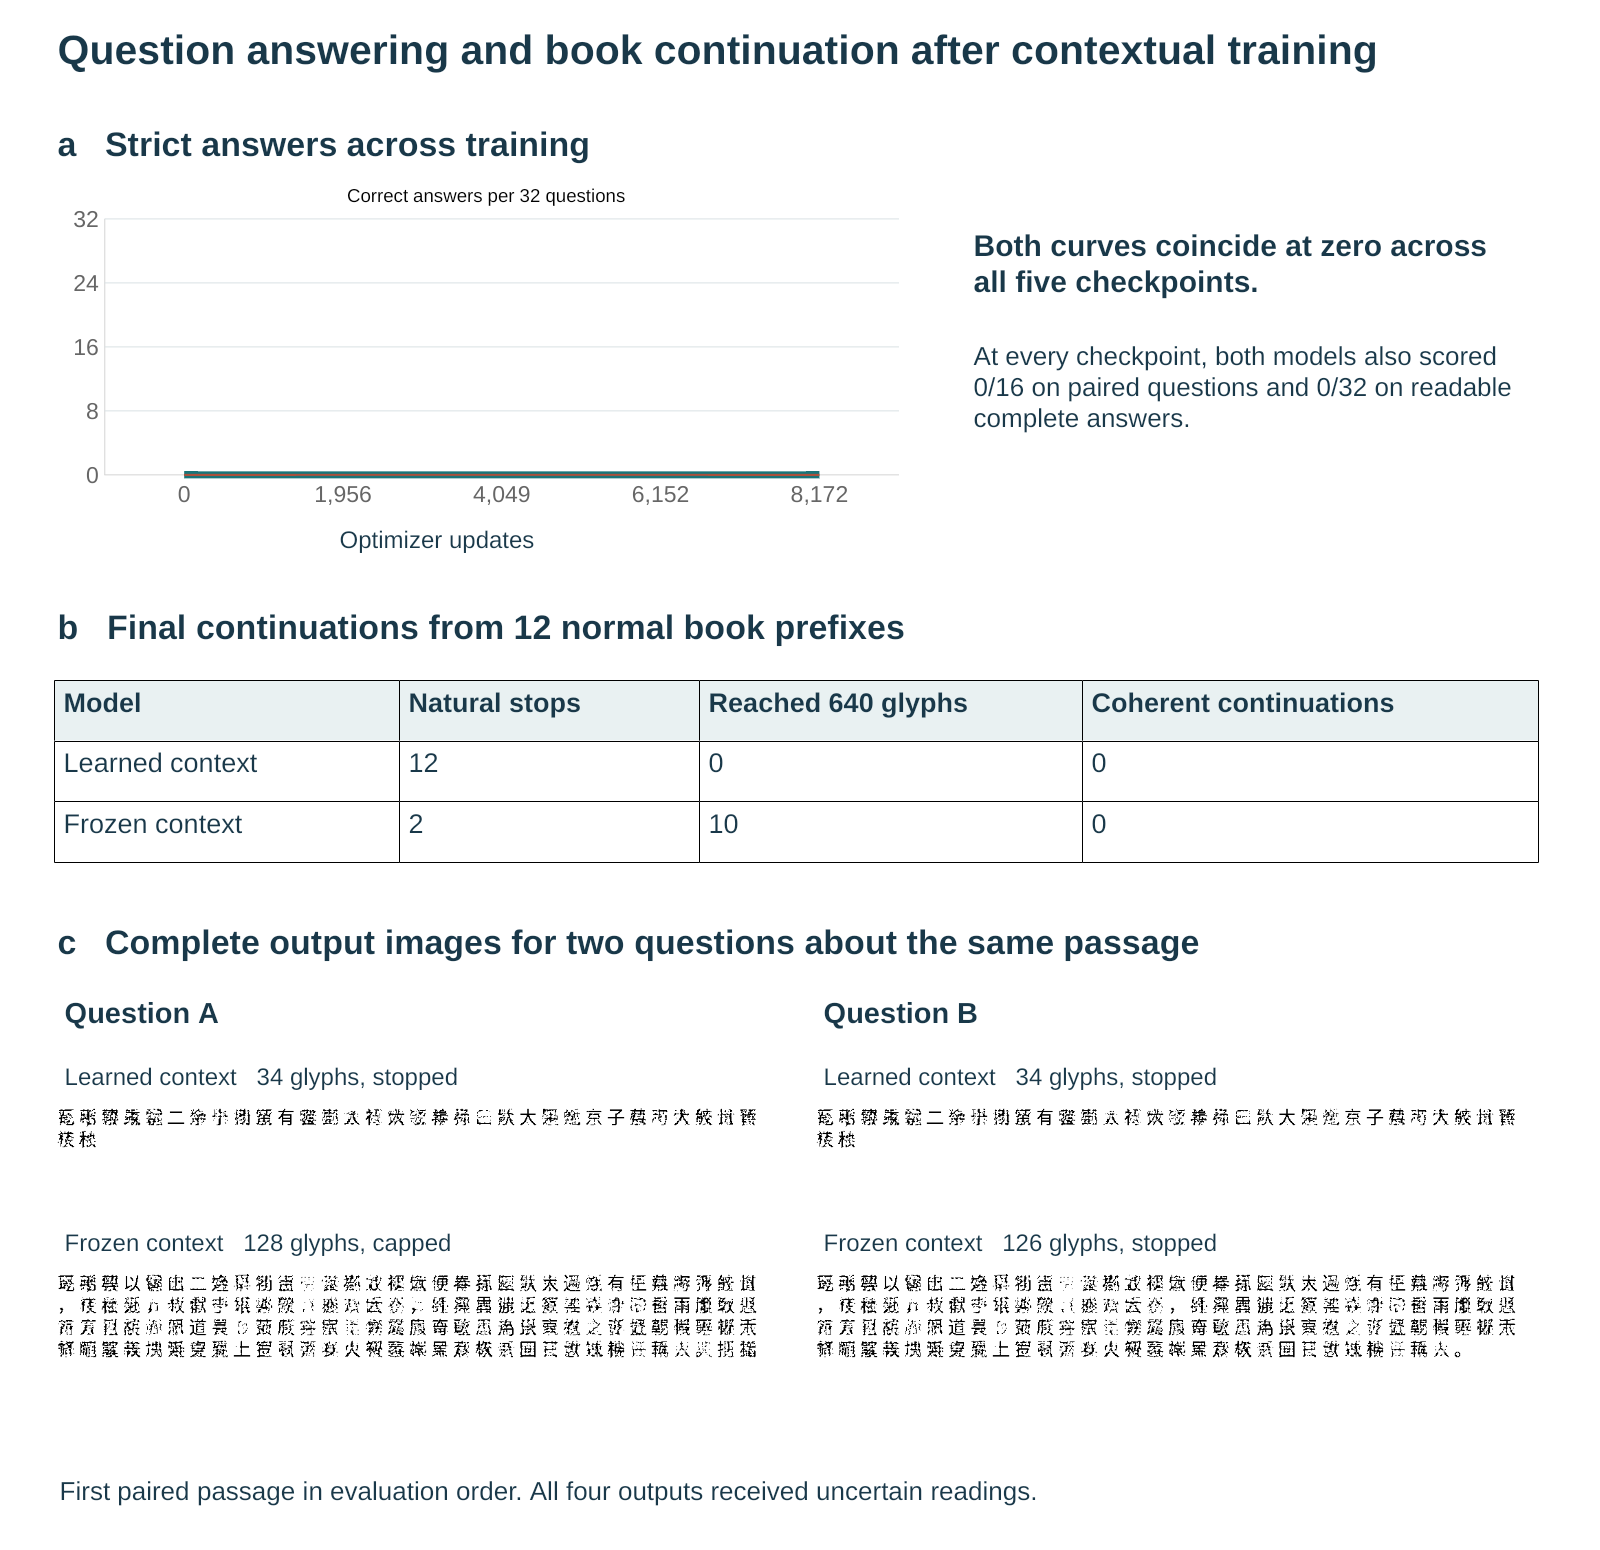
\includegraphics[width=.84\textwidth]{figures/Figure_32_full_context_comparison.png}
\caption{\DIFaddFL{\textbf{Context training changes termination while complete answers remain unreadable.}
\textbf{a,} Correct normal answers at the five prescribed checkpoints for the learned
and frozen contextual bodies. Both curves lie at zero. The 32 questions form 16
same-passage pairs. \textbf{b,} Final outcomes for the twelve normal long-book
prefixes. Capped outputs retain all 640 emitted positions.
\textbf{c,} Complete final images for the first paired passage in evaluation order.
The learned model stops after 34 positions for both questions. The frozen model
reaches the cap on the first question and stops after 126 positions on the second.
The blinded reader marked all four answers uncertain.}}
\label{fig:full-context-comparison}
\end{figure*}
\begin{figure*}[p]
\centering
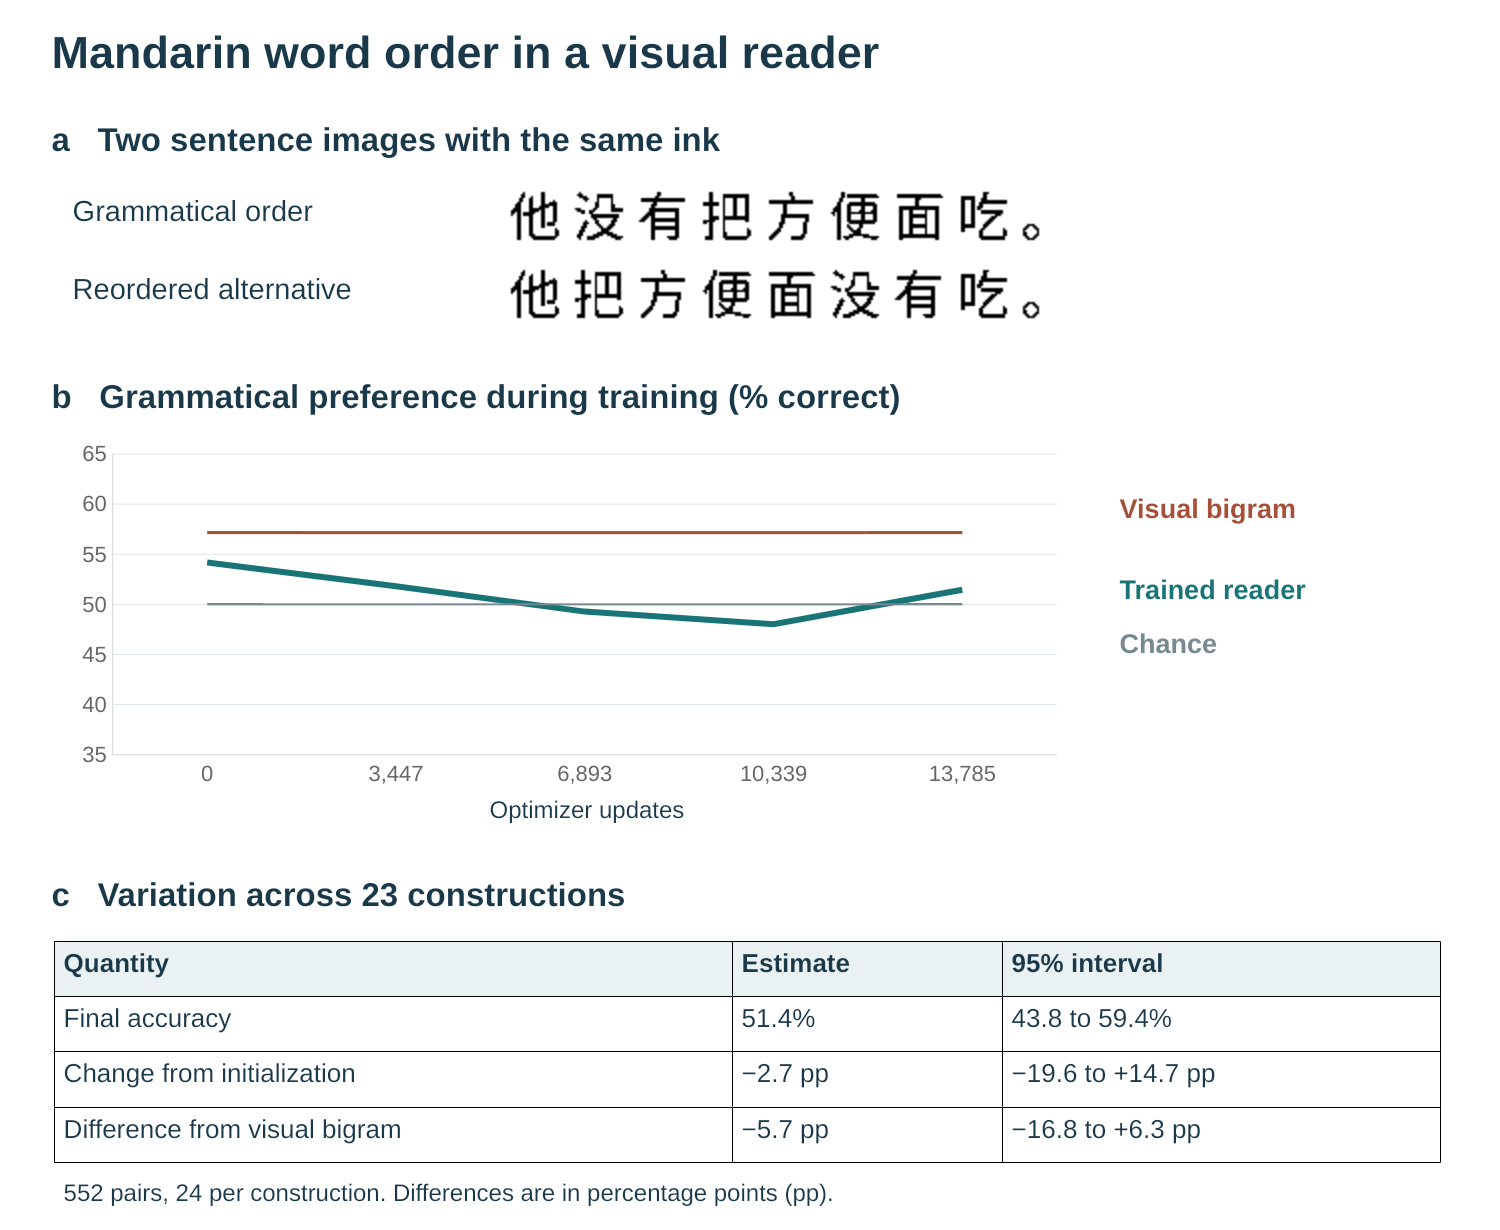
\includegraphics[width=.84\textwidth]{figures/Figure_33_visual_word_order.png}
\caption{\DIFaddFL{\textbf{Grammatical order preference across five visual-reader checkpoints.}
\textbf{a,} Both complete input images from the first selected benchmark pair
(ZhoBLiMP, negation in the Mandarin \emph{ba} construction). They preserve the
same first glyph and the same physical cells. \textbf{b,} The native reader
scores the grammatical order higher in 299, 286, 272, 265 and 284 of the same
552 pairs. The full-corpus bigram is shown as a fixed reference. It wins
288 comparisons and ties 55. \textbf{c,} Estimates and descriptive 95\%
intervals from paired resampling of 23 paradigms. A tie receives half credit.}}
\label{fig:visual-word-order}
\end{figure*}
\begin{figure*}[p]
\centering
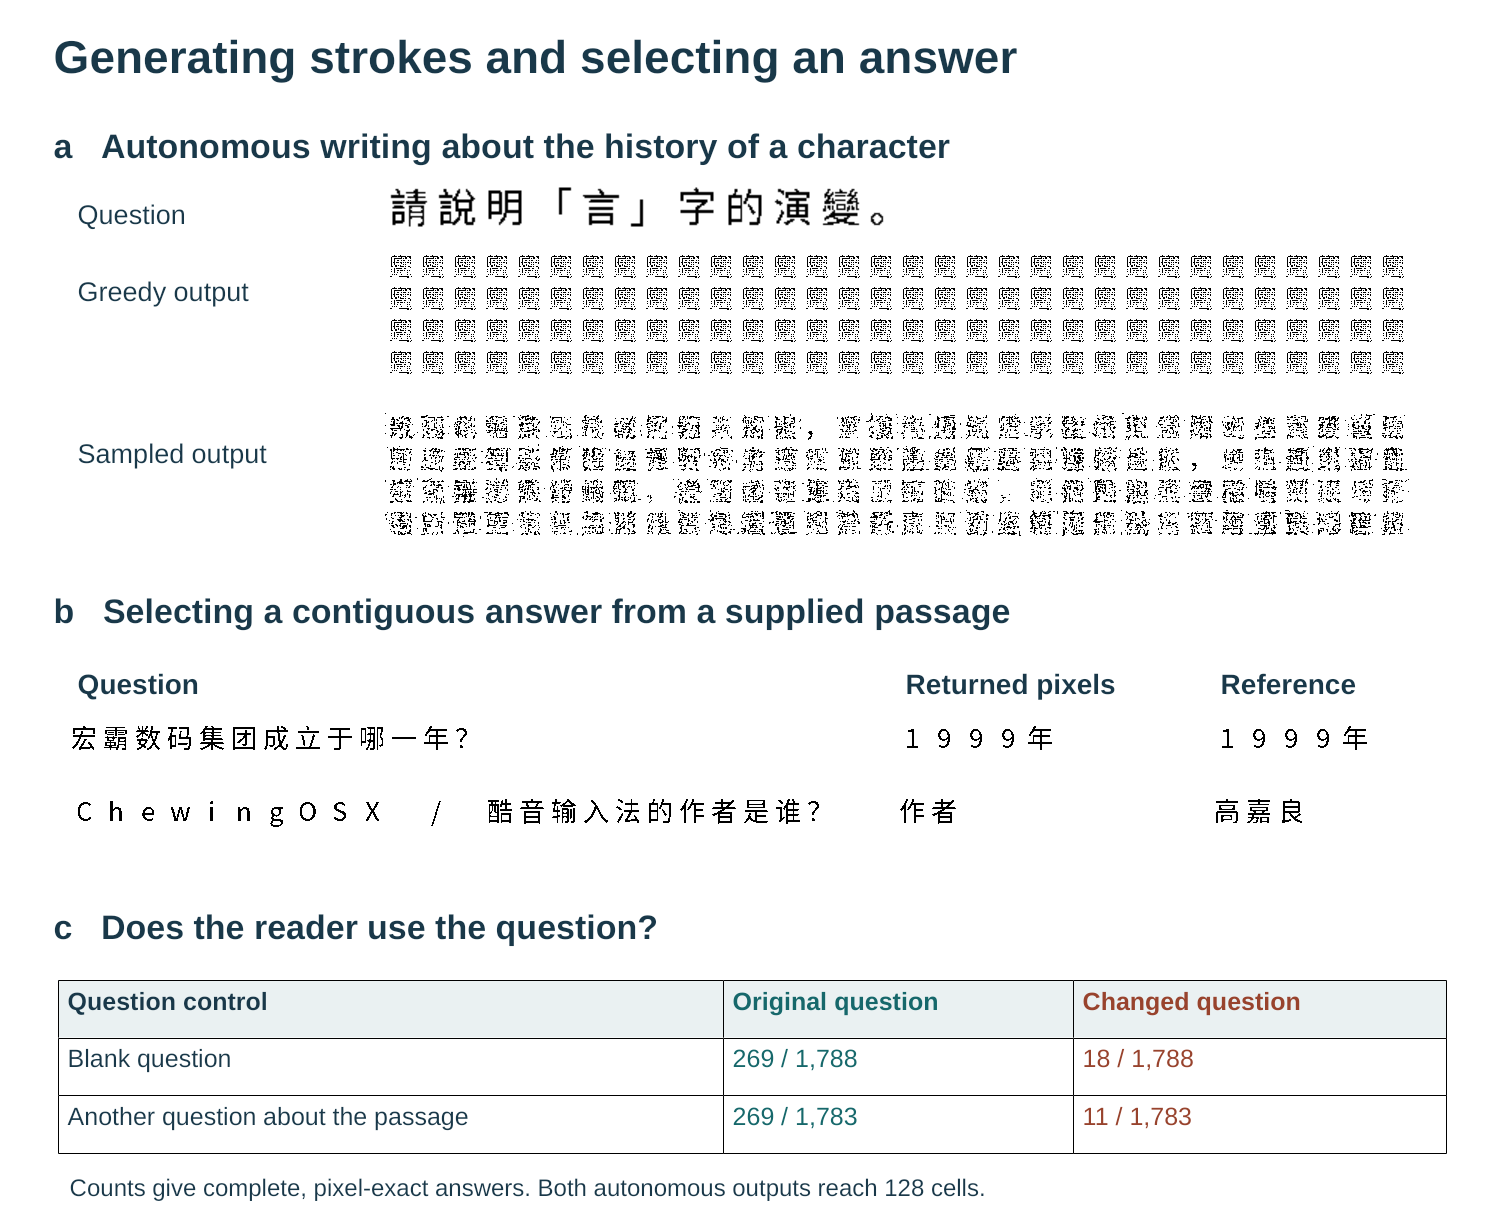
\includegraphics[width=.84\textwidth]{figures/Figure_34_visual_reading_writing.png}
\caption{\DIFaddFL{\textbf{Autonomous writing and evidence selection in Chinese.}
\textbf{a}, The full question asks for the evolution of the character for
speech. Greedy and sampled writing use the same 23.55-million-parameter
checkpoint. Both reach 128 cells. Neither image conveys a readable account.
\textbf{b}, A separate reader selects answer pixels from a supplied passage.
The first correct case in the fixed test order asks for a founding year. The
first case overall asks for an author's name. Here the reader selects the
word for author. The original question, output and reference images retain
their strokes. \textbf{c}, The same reader receives either its original
question, white cells of equal length or a different question about the same
passage. Five questions lack a changed counterpart under cyclic exchange.}}
\label{fig:visual-reading-writing}
\end{figure*}
\begin{figure*}[p]
\centering
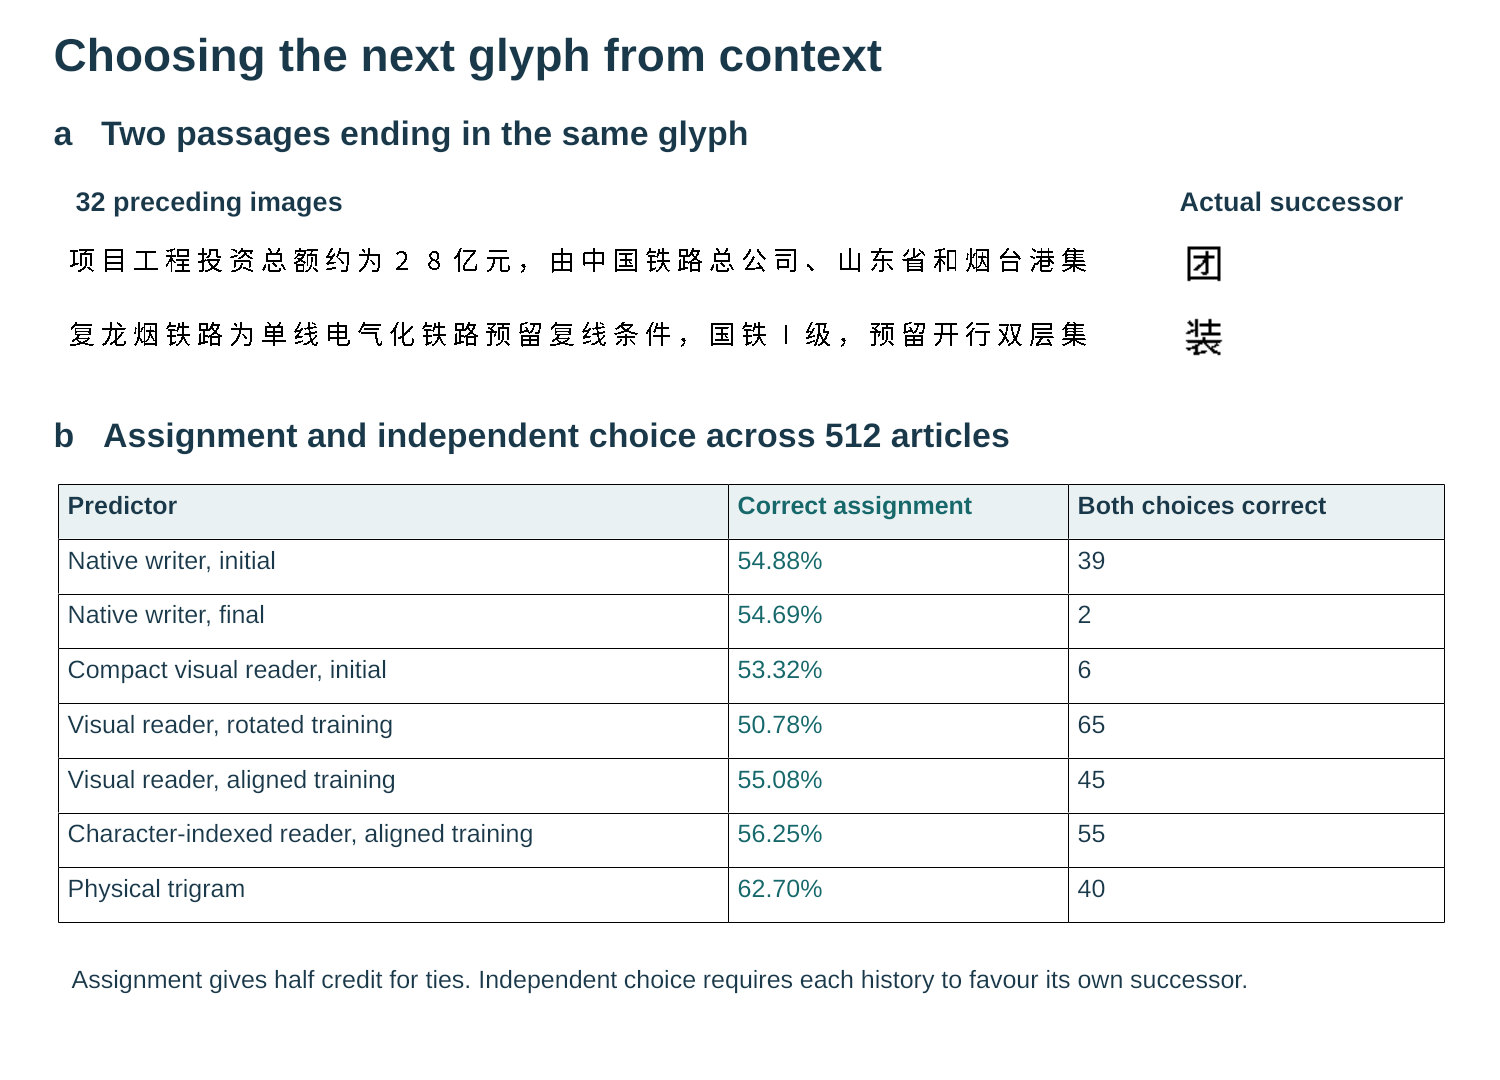
\includegraphics[width=.84\textwidth]{figures/Figure_35_visual_successors.png}
\caption{\DIFaddFL{\textbf{Selecting the next glyph from two pictured alternatives.}
\textbf{a}, The two 32-image histories and their reference successors from
the first article in the fixed order. Each successor is absent from both
histories. \textbf{b}, Joint assignment compares the two possible pairings.
The final column counts articles where the two histories independently
assign their highest score to their own successor. The physical trigram tied
on 288 assignments. The three compact readers with explicit supervision
saw identical training passages and update counts. The native writer learned from book continuations
and QA answers, with modern passages appearing inside its input prompts. Chance for joint assignment is 50\%.}}
\label{fig:visual-successors}
\end{figure*}
\begin{figure*}[p]
\centering
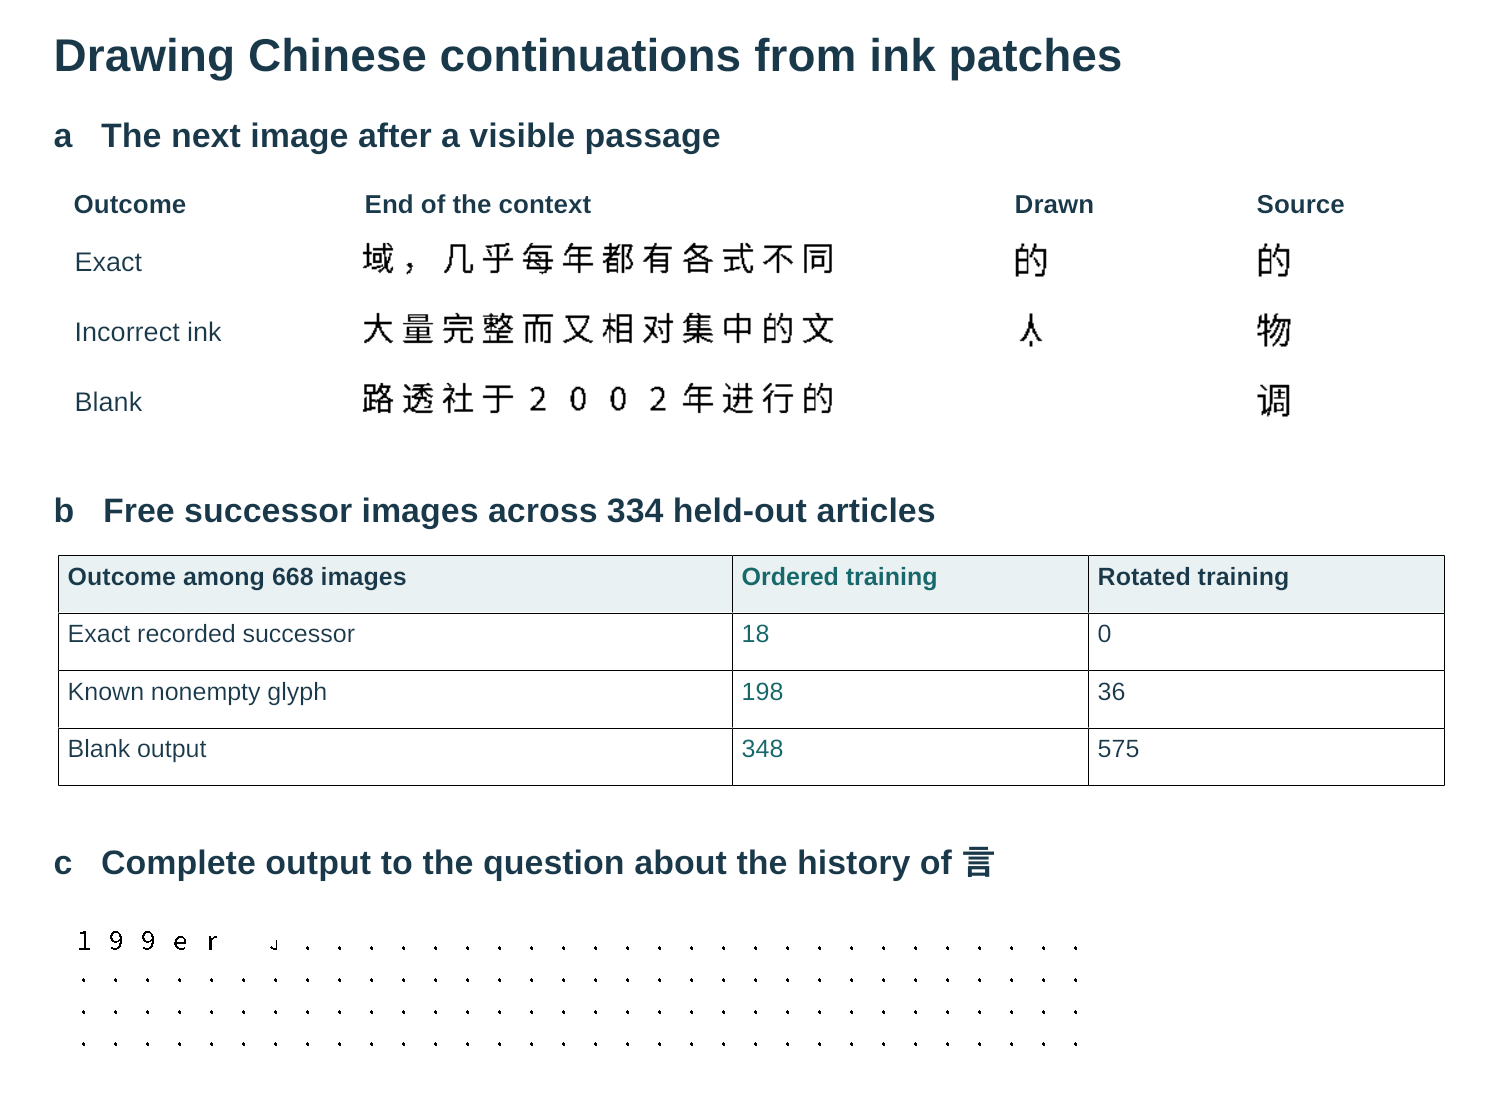
\includegraphics[width=.84\textwidth]{figures/Figure_36_patch_writing.png}
\caption{\DIFaddFL{\textbf{Free next-glyph drawing from local visual context.}
\textbf{a}, The first exact, first nonempty incorrect and first blank
response in fixed article order. Each strip shows the last twelve cells
observed. The white output cell in the last row is the actual drawing.
\textbf{b}, Counts from 668 independently generated next images. A known
nonempty glyph exactly matches a nonempty bitmap in the training repertoire.
The control retained the observed frequencies of complete images and spatial
patch joins. \textbf{c}, Complete output of the ordered model to the
pictured etymology question. It reached the 128-cell limit.}}
\label{fig:patch-writing}
\end{figure*}
\begin{figure*}[p]
\centering
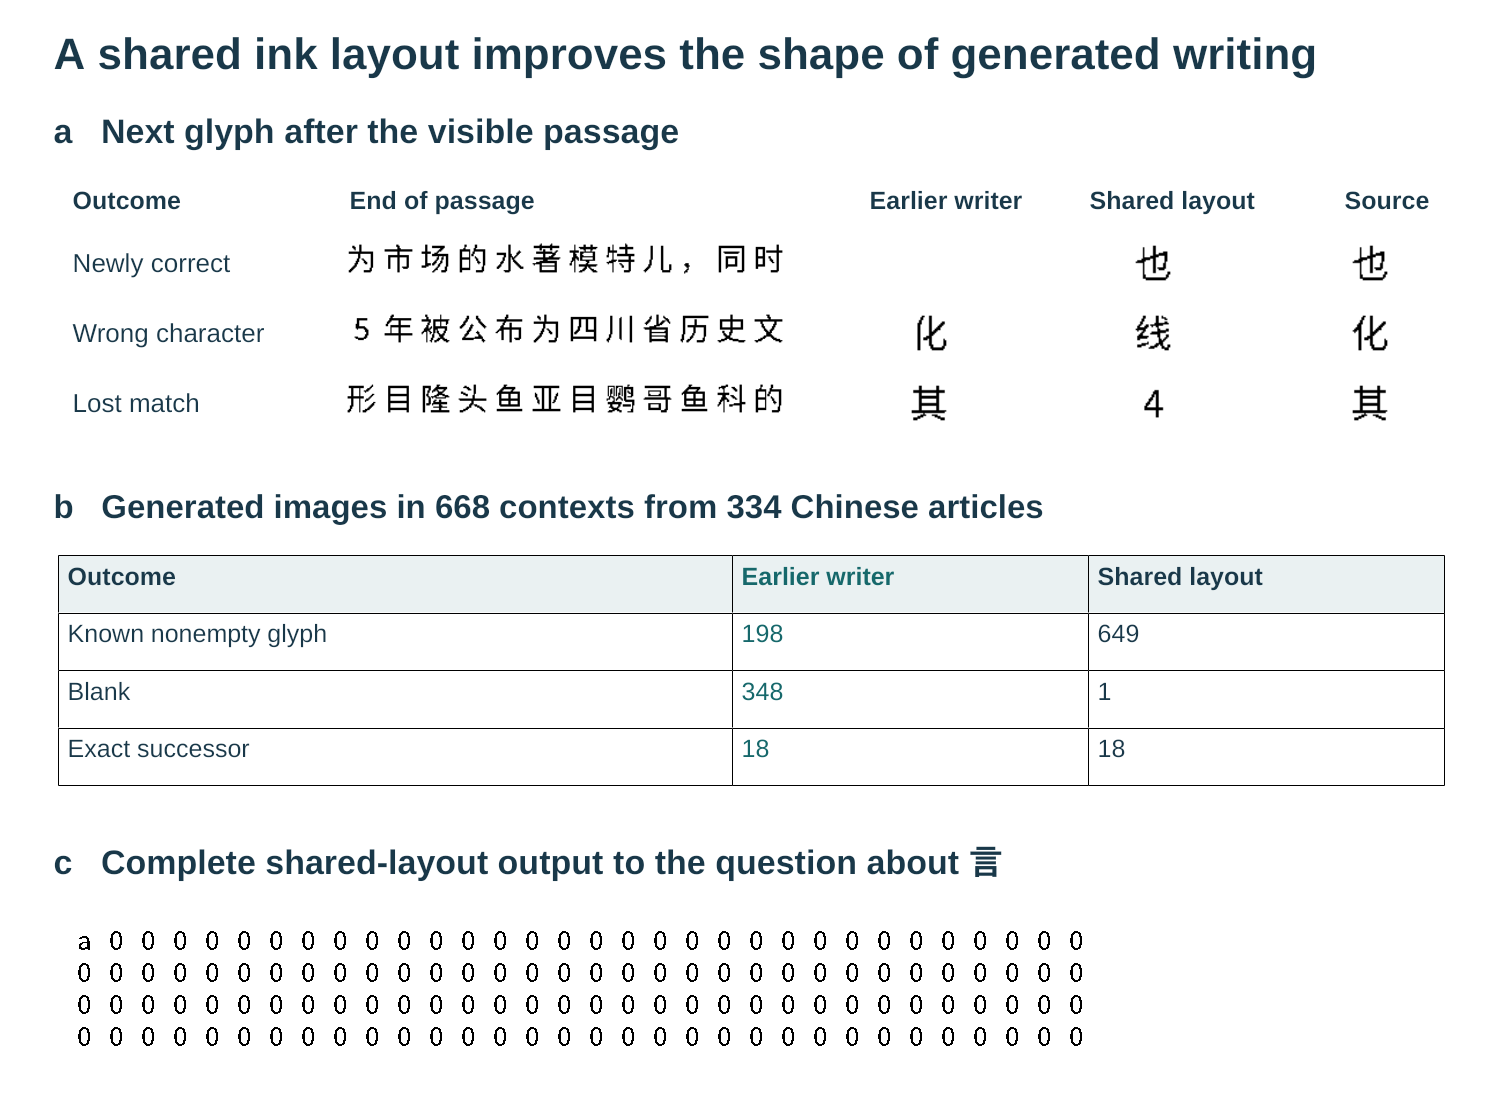
\includegraphics[width=.84\textwidth]{figures/Figure_37_shared_layout.png}
\caption{\DIFaddFL{\textbf{A shared physical layout improves glyph fidelity.}
\textbf{a}, Original images from matched pictured contexts. The rows show
the first newly correct output, the first incorrect match to a known Han
bitmap after an earlier output outside that set, and the first lost match
in article order. The source
continues with a different character in the second row.
\textbf{b}, Complete counts under the two ordered writers. A known
nonempty glyph may also be a digit, letter or punctuation mark.
\textbf{c}, The entire response to the pictured etymology question begins
with a lowercase letter and repeats an oval to the 128-cell cap.}}
\label{fig:shared-layout}
\end{figure*}
\begin{figure*}[p]
\centering
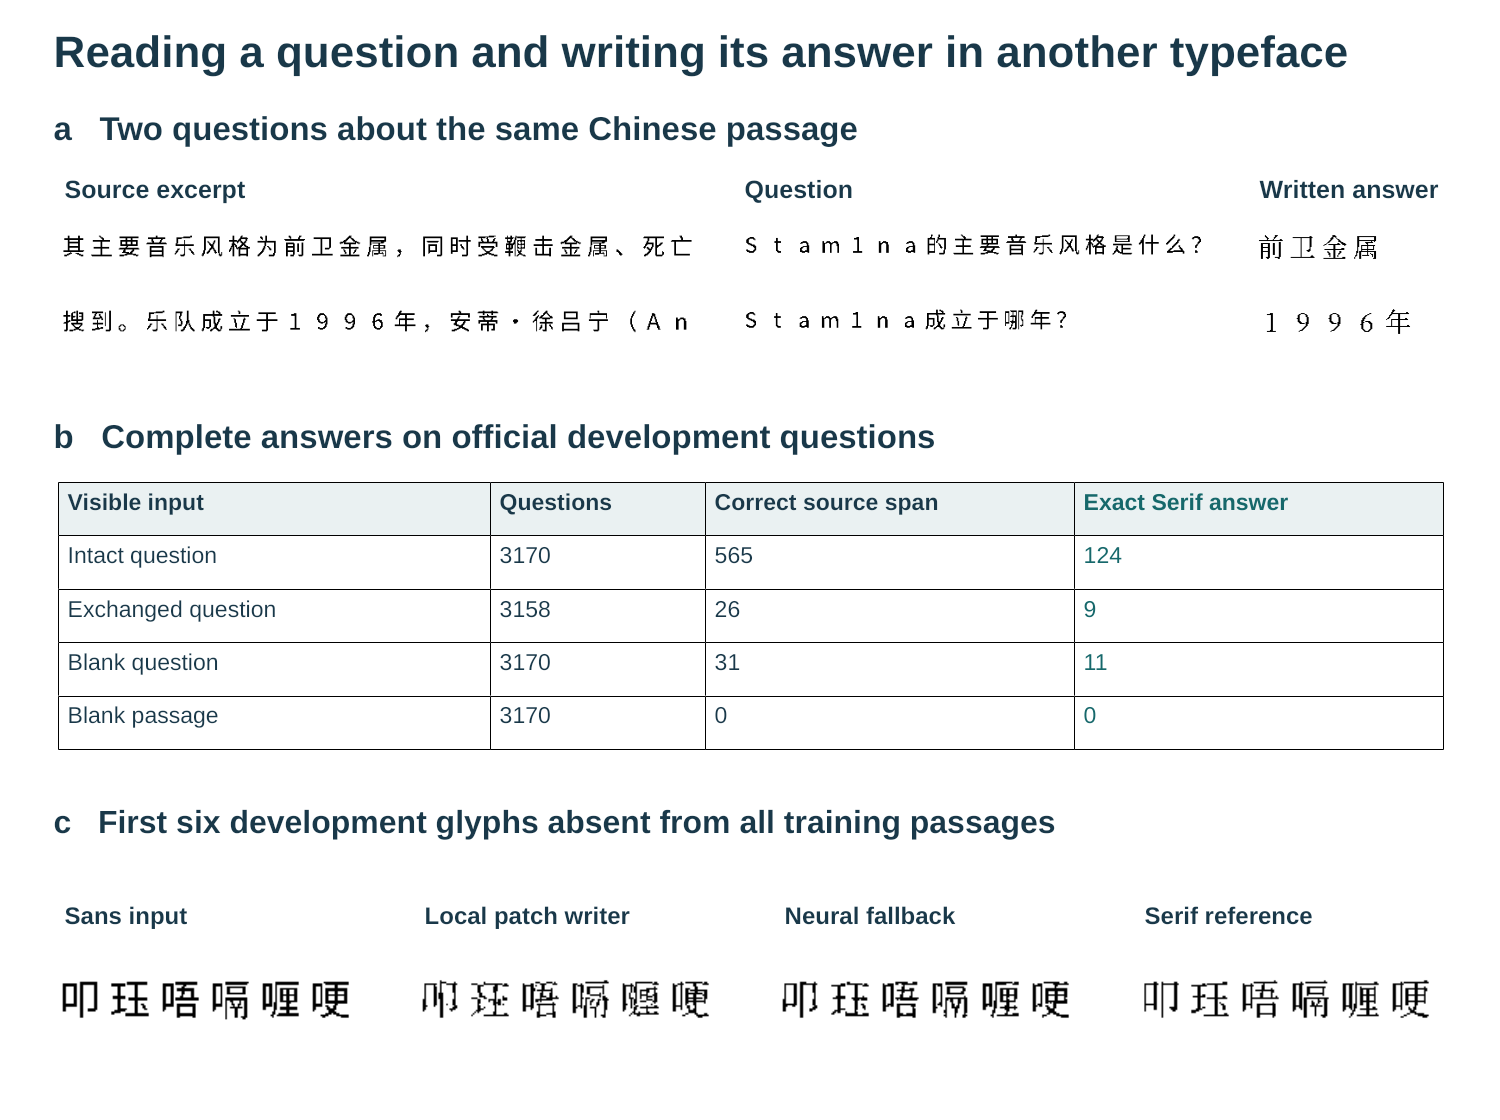
\includegraphics[width=.84\textwidth]{figures/Figure_38_grounded_detail.png}
\caption{\DIFaddFL{\textbf{Cross-typeface writing from the same pictured passage.}
\textbf{a}, Two original input excerpts and questions in Sans and the complete
model outputs in Serif. One question asks the musical style of the band
Stam1na; the other asks its founding year. This is the first eligible pair
with two different correct responses in the registered order.
\textbf{b}, A correct source span matches a human reference in Sans.
An exact written answer matches a complete human reference in Serif.
\textbf{c}, The first six Han glyphs in bitmap order among 314 development
shapes absent from the training passages. The neural fallback supplies local
detail when the count writer has no matching neighbourhood and layout.}}
\label{fig:grounded-detail}
\end{figure*}
\begin{figure*}[p]
\centering
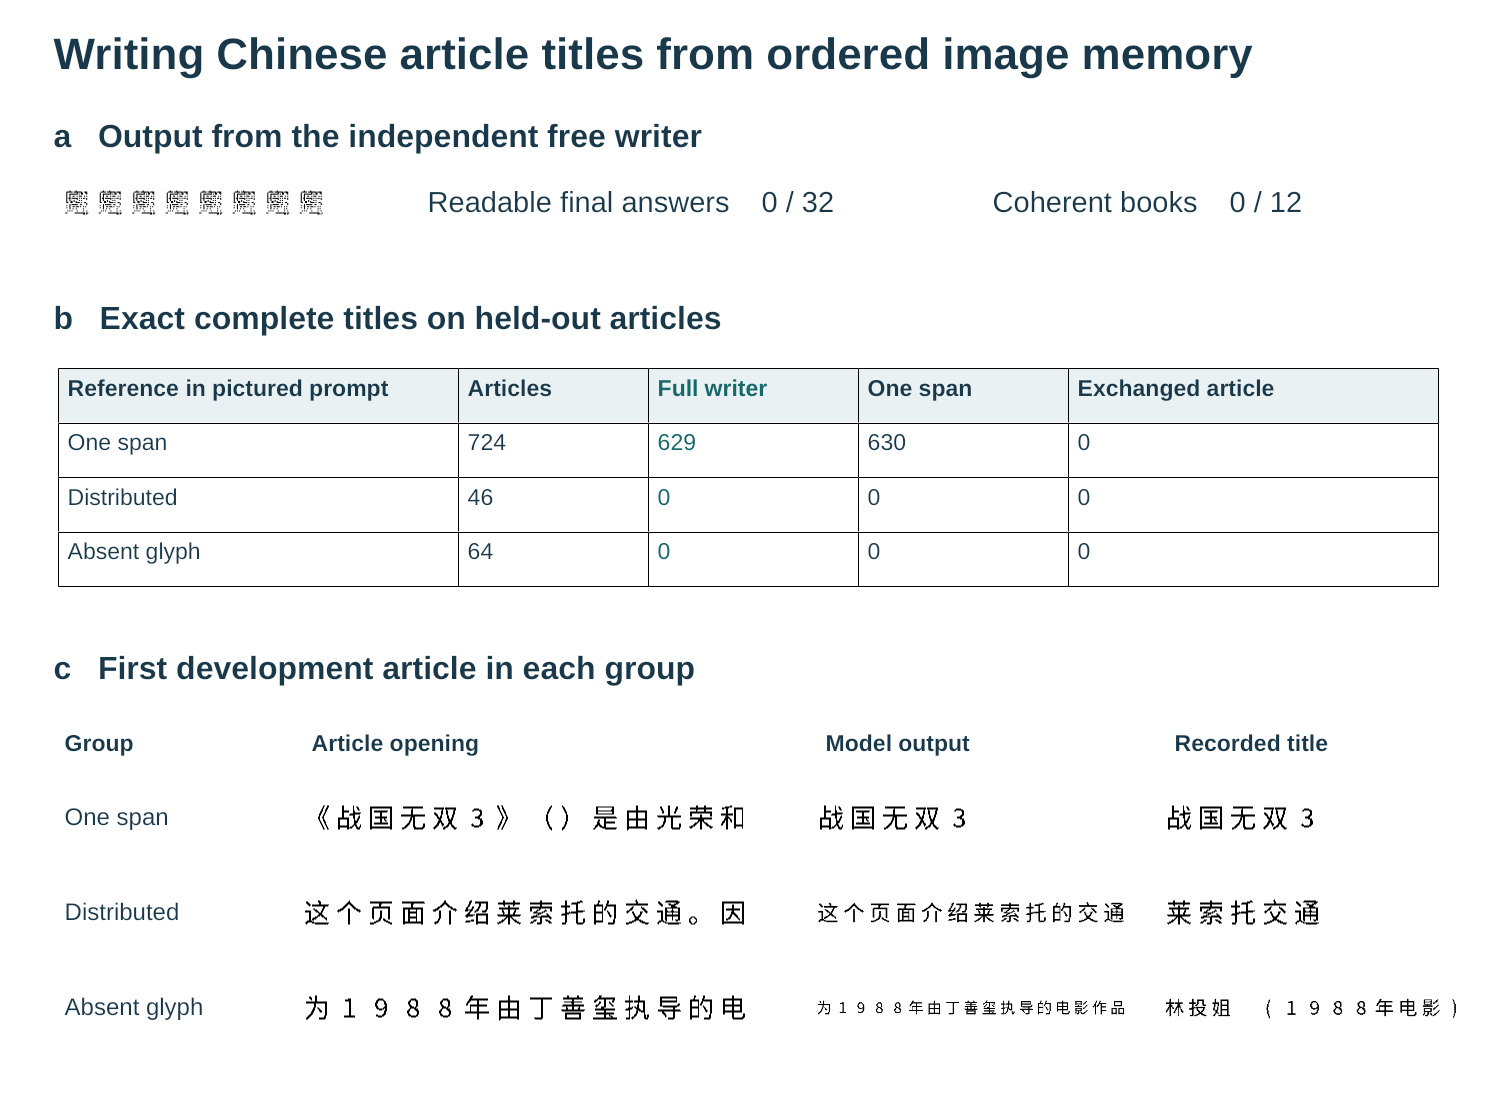
\includegraphics[width=.84\textwidth]{figures/Figure_39_visual_titles.png}
\caption{\DIFaddFL{\textbf{Article-title prediction from pictured Chinese.}
\textbf{a}, A prefix of eight emitted cells from the first normal short
question in the final eight-component free-writing evaluation (case order).
The blind evaluation used the complete original streams.
\textbf{b}, Complete titles with an autonomous stop and pixel-for-pixel
agreement with the recorded reference. The contiguous control uses the same
trained transducer with a single source interval. The exchanged control
receives the next article in the fixed roster.
\textbf{c}, Original output and reference images for the first development
article in each group. The source column shows only the beginning of the
article. All models receive the full pictured input.}}
\label{fig:visual-titles}
\end{figure*}
\begin{figure*}[p]
\centering
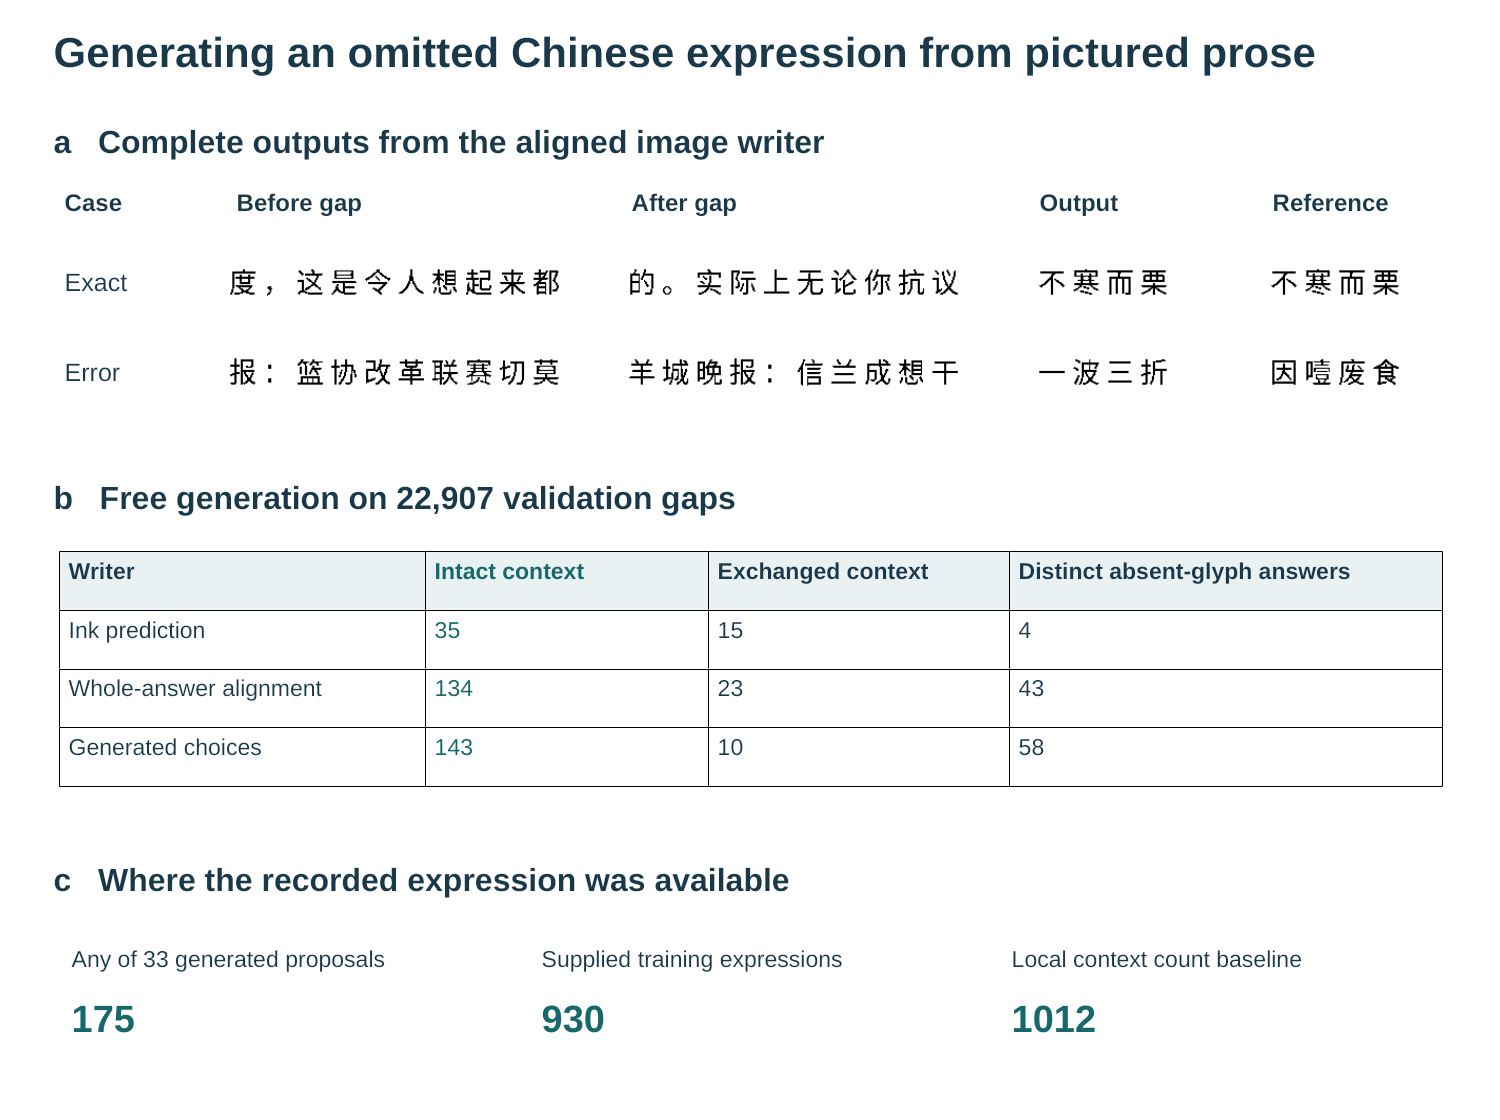
\includegraphics[width=.84\textwidth]{figures/Figure_40_pictured_idioms.png}
\caption{\DIFaddFL{\textbf{An omitted idiom generated as four Han images.}
\textbf{a}, The first exact aligned completion for which all four target
characters were absent from the visible window, and the first error in
validation order. Ten of the 24 visible cells on each side of the gap
are shown. Each output and reference is complete.
\textbf{b}, Complete exact stopped outputs with intact or cyclically
exchanged contexts. The final column counts distinct correct expressions
with at least one missing target glyph.
\textbf{c}, The number of gaps for which any of the 33 generated proposals
was correct; exact selections when the reader was supplied all 3,805
training expressions; and exact answers from a local count model. Each
control was evaluated on all 22,907 windows.}}
\label{fig:pictured-idioms}
\end{figure*}
\begin{figure*}[p]
\centering
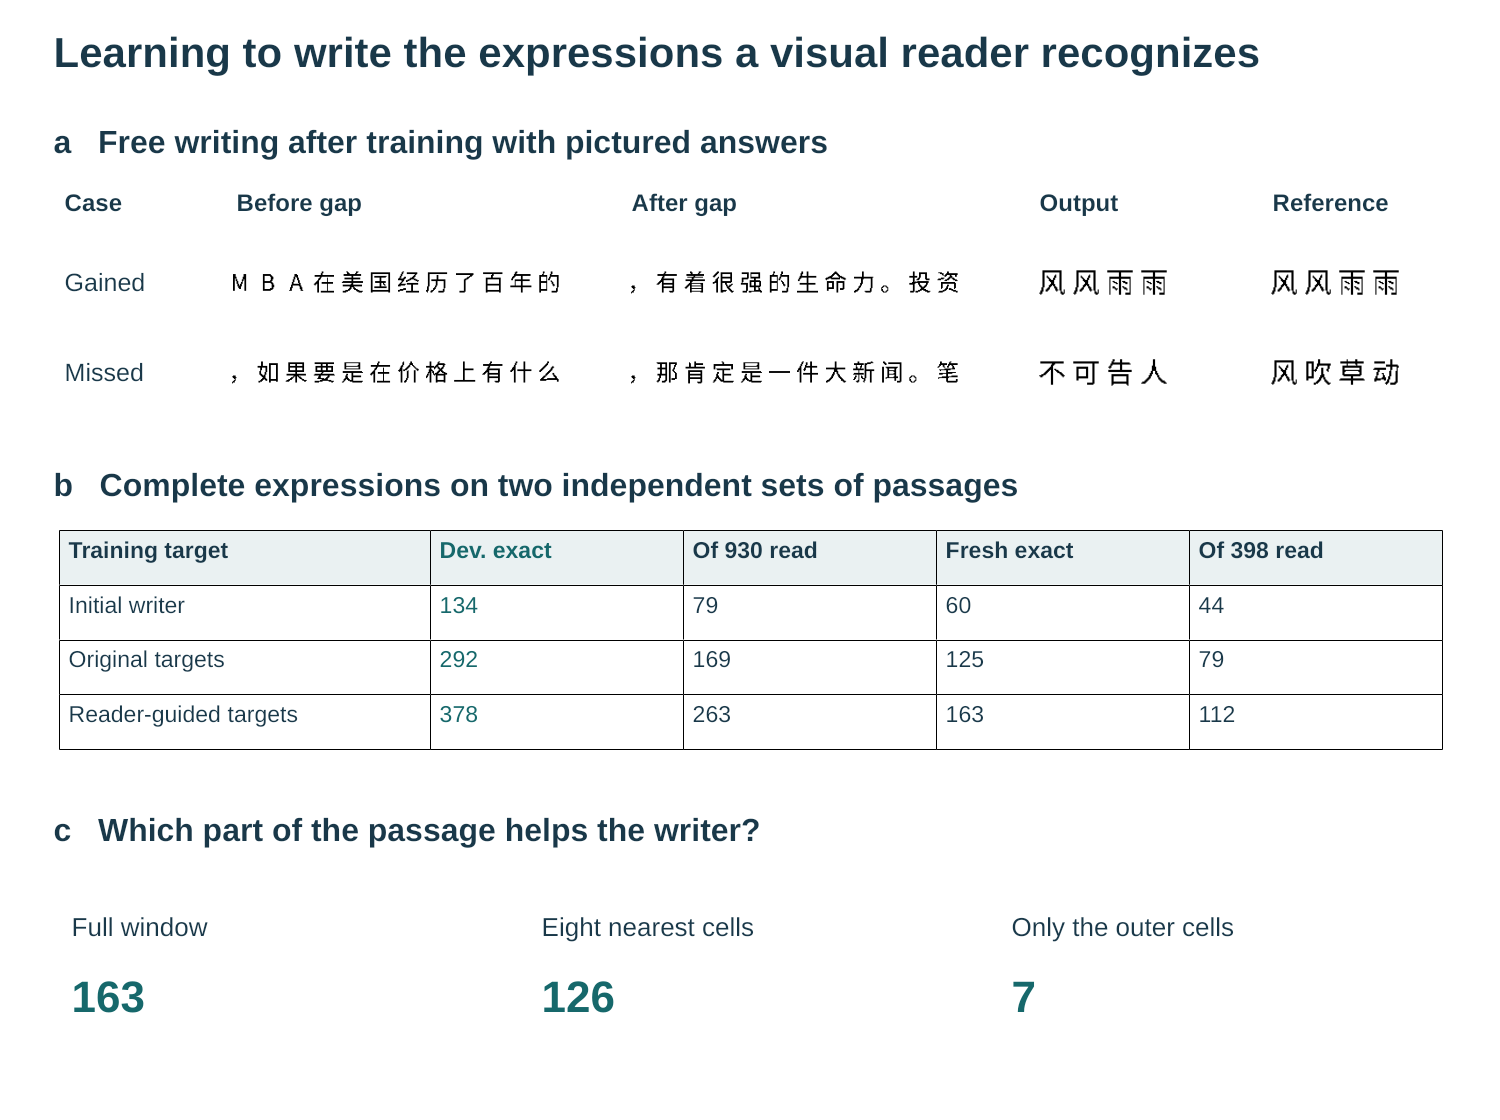
\includegraphics[width=.84\textwidth]{figures/Figure_41_writer_transfer.png}
\caption{\DIFaddFL{\textbf{Teaching the writer with pictures scored by the frozen reader.}
\textbf{a}, First newly exact development answer and first remaining error among answers the reader recognized. Twelve cells on each side of the gap and the complete output and reference are shown.
\textbf{b}, Exact stopped outputs on 22,907 development passages and 9,135 previously unused passages. The subset columns count exact outputs on the 930 and 398 respective cases answered correctly by the frozen reader when supplied pictured options. The two continued fits used identical schedules.
\textbf{c}, Exact outputs on the same 9,135 passages after retaining all 48 input slots, retaining only the eight nearest slots or erasing those eight. All three evaluations used the same final reader-guided writer.}}
\label{fig:writer-transfer}
\end{figure*}
\begin{figure*}[p]
\centering
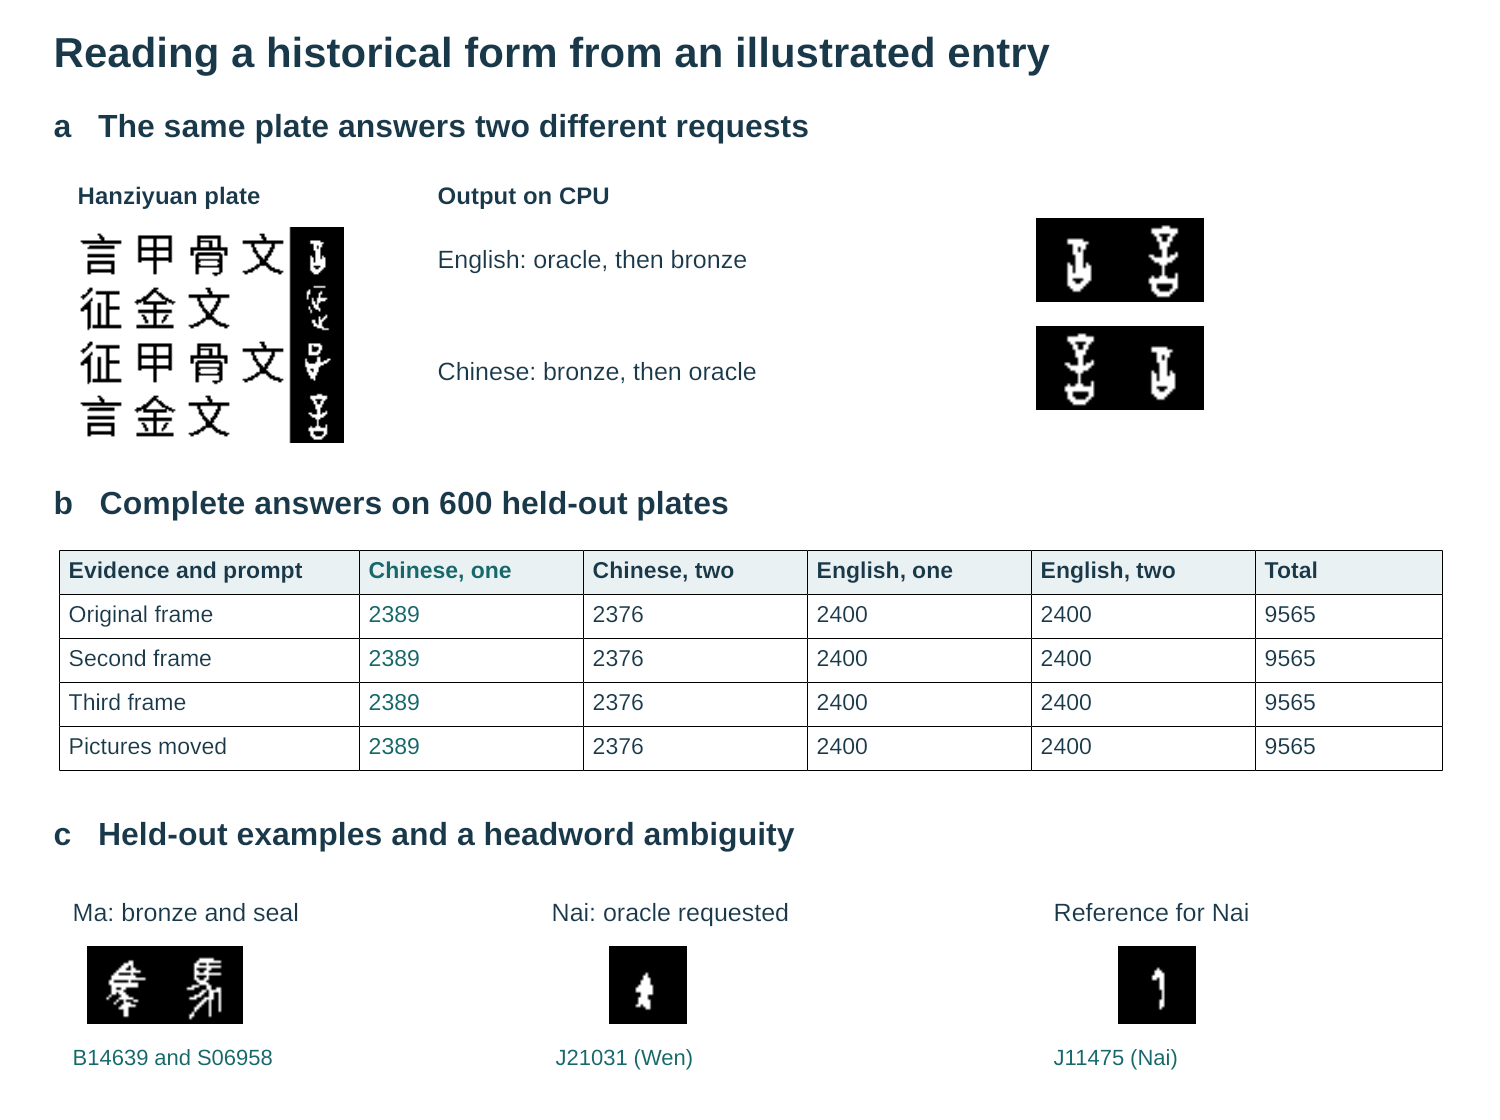
\includegraphics[width=.84\textwidth]{figures/Figure_42_historical_plates.png}
\caption{\DIFaddFL{\textbf{Bilingual instructions select historical forms from visible evidence.}
\textbf{a}, A training-family plate for Yan and Zheng. Two fresh CPU invocations return the same attested oracle and bronze images in the requested orders. Each output is enlarged from its stored pixels.
\textbf{b}, Exact stopped answers on 600 development plates. Each subgroup contains 2,400 requests. The three frames share the same evidence and stage names. In the final row all historical images move to different labelled rows, and the reference follows the new location.
\textbf{c}, The first development two-stage request returns the bronze and seal forms of Ma. The first error returns the oracle form of Wen when asked for that of Nai. The competing headword occurs within the Chinese stage name.}}
\label{fig:historical-plates}
\end{figure*}
\begin{figure*}[p]
\centering
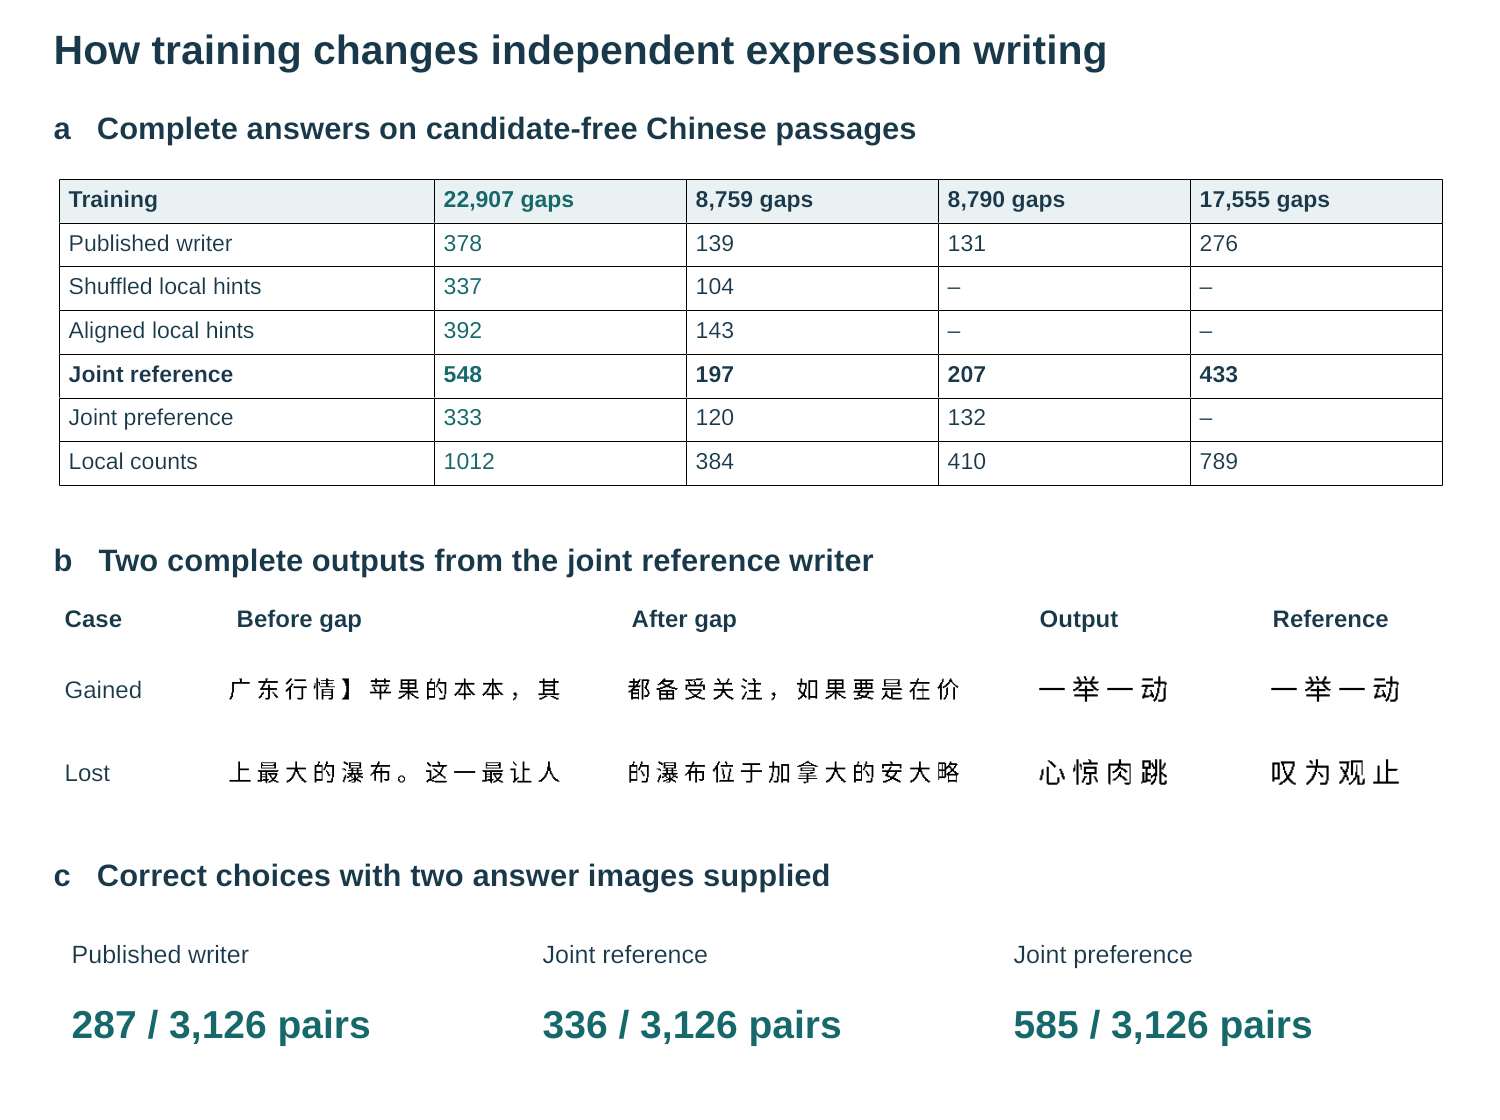
\includegraphics[width=.84\textwidth]{figures/Figure_43_expression_preference.png}
\caption{\DIFaddFL{\textbf{Conditional scoring and independent writing after two changes to supervision.}
\textbf{a}, Counts of exact complete stopped expressions. Columns show official development and three disjoint sets of source groups, in order of first assessment. The final column was opened after freezing the joint reference writer. Dashes indicate unevaluated combinations. The count baseline returns a training expression from neighboring images.
\textbf{b}, First validation gain and loss of the joint reference writer relative to the published guided writer. Twelve cells from each side of the gap and the full generated and reference images are shown.
\textbf{c}, Both recorded expressions preferred to their exchanged alternatives for the same 3,126 matched pairs of passages. This diagnostic supplies the two physical answer trajectories to be scored. Panel a measures autonomous generation.}}
\label{fig:expression-preference}
\end{figure*}
\begin{figure*}[p]
\centering
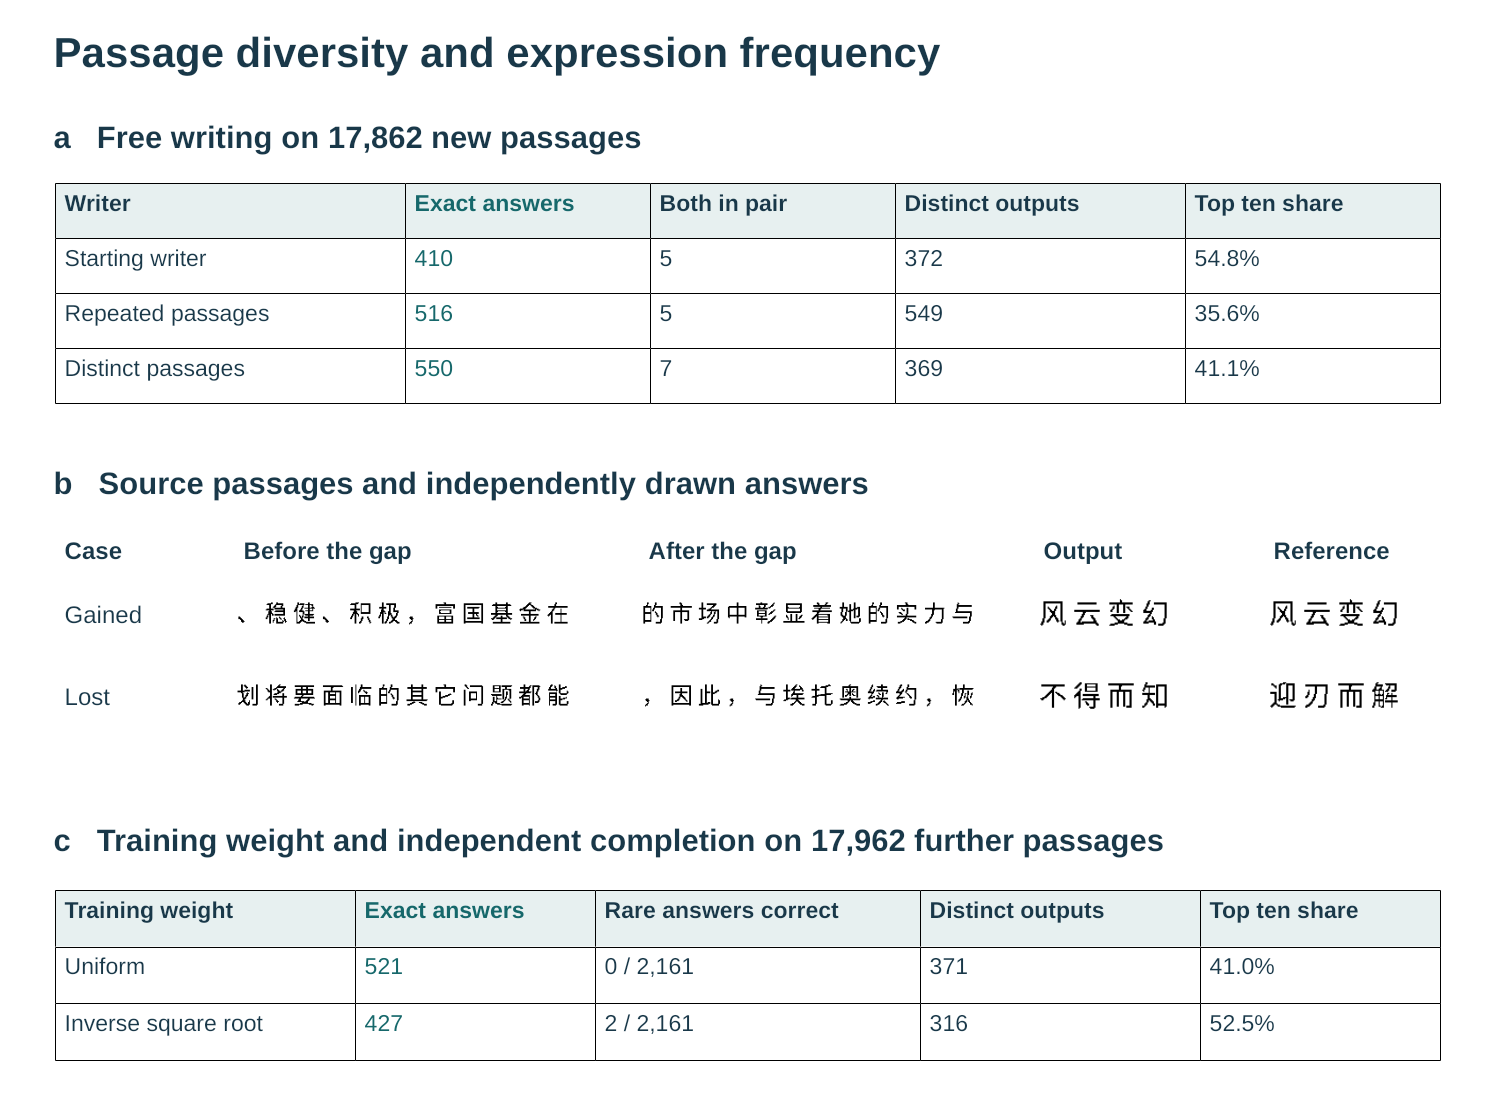
\includegraphics[width=.84\textwidth]{figures/Figure_44_passage_diversity.png}
\caption{\DIFaddFL{\textbf{Passage diversity and expression frequency under a fixed training budget.}
\textbf{a}, Exact stopped answers and output diversity on 17,862 held-out passages. Both in pair counts pairs with two exact answers among 6,772 pairs sharing the glyphs at the gap boundary. Top ten share is the fraction of all cases assigned to the ten most frequent outputs.
\textbf{b}, First source-order gain and loss from training with additional distinct passages relative to repeating the original corpus. The panel shows twelve pictured cells from each side of the gap and the complete emitted and source expressions.
\textbf{c}, Uniform and frequency-weighted likelihood on 17,962 further held-out passages. Rare answers occurred one to twenty times in the combined training data.}}
\label{fig:passage-diversity}
\end{figure*}
\begin{figure*}[p]
\centering
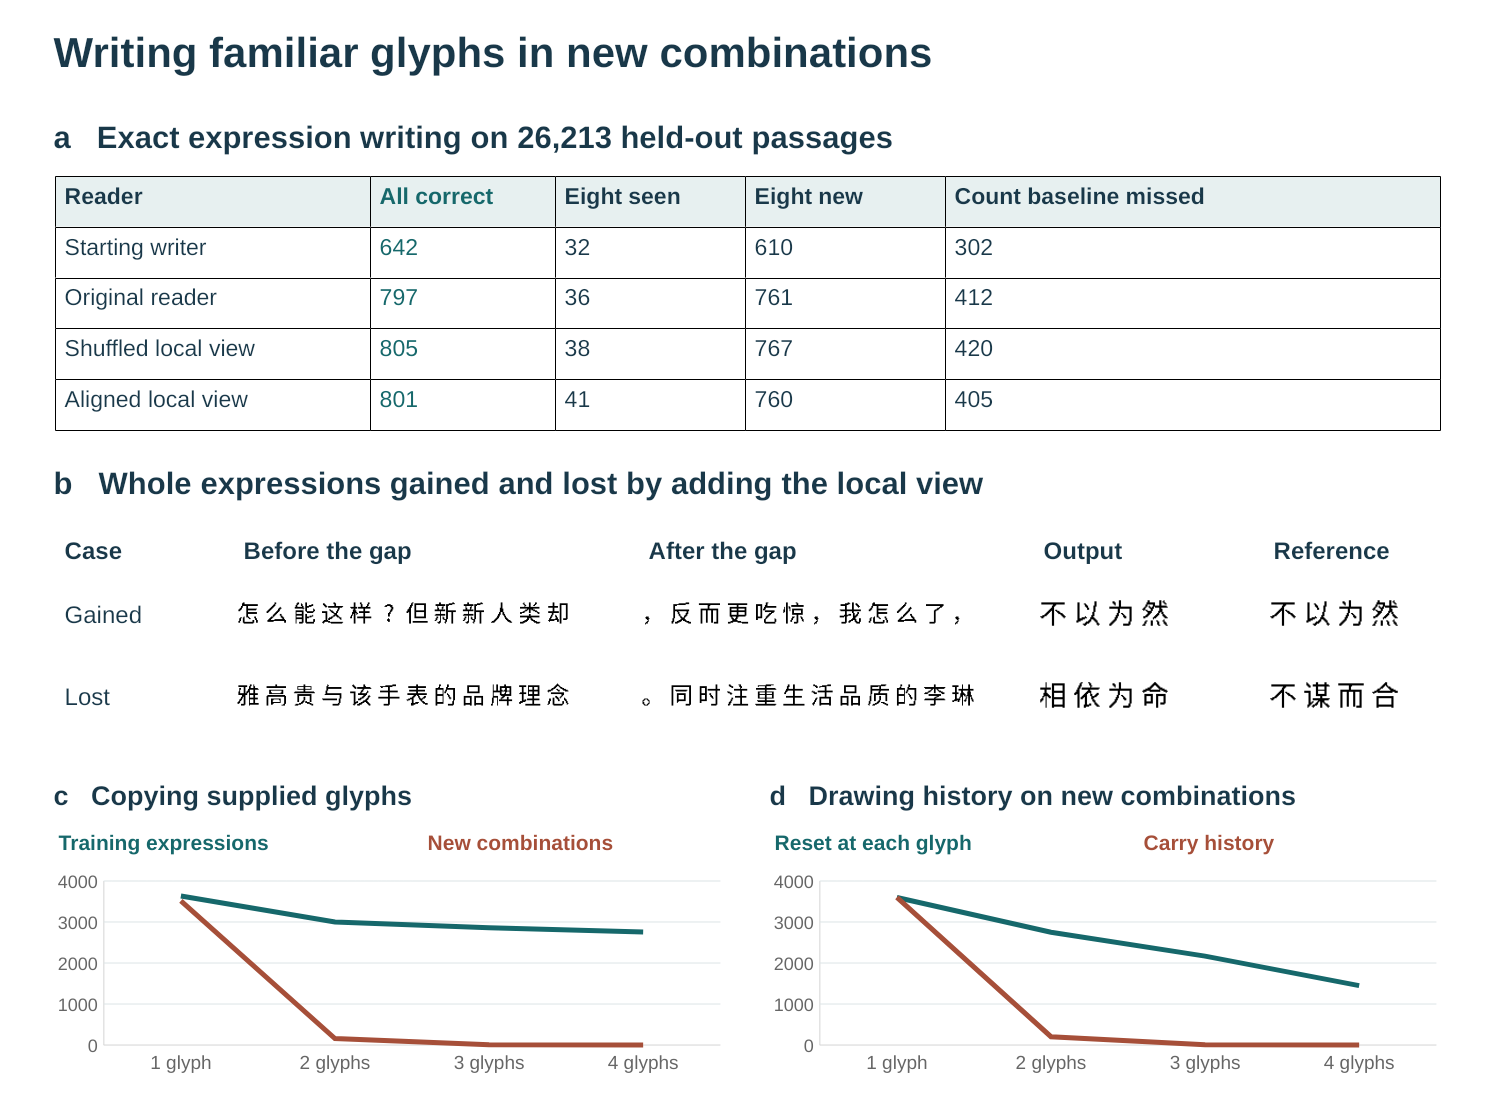
\includegraphics[width=.84\textwidth]{figures/Figure_45_ordered_neighborhood.png}
\caption{\DIFaddFL{\textbf{Passage-conditioned writing and copying of unfamiliar glyph combinations.}
\textbf{a}, Complete pixel-exact expressions on 26,213 held-out passages. Eight seen and eight new distinguish local windows present or absent in training. The last column counts correct answers on cases missed by local counts.
\textbf{b}, First gain and loss in source order relative to the original reader, with the local context, actual output and reference pixels.
\textbf{c}, Number of exactly copied prefixes at each length for 3,845 training expressions and 3,845 previously unseen combinations. Each target glyph was supplied to the shared controller as an image during this copying test.
\textbf{d}, On the same unfamiliar combinations, both arms received four output positions and committed one path per glyph. Clearing drawing history changed the number of complete copies from zero to 1,450. Curves in c and d show the number of strings correct through the indicated glyph.}}
\label{fig:ordered-neighborhood}
\end{figure*}
\begin{figure*}[p]
\centering
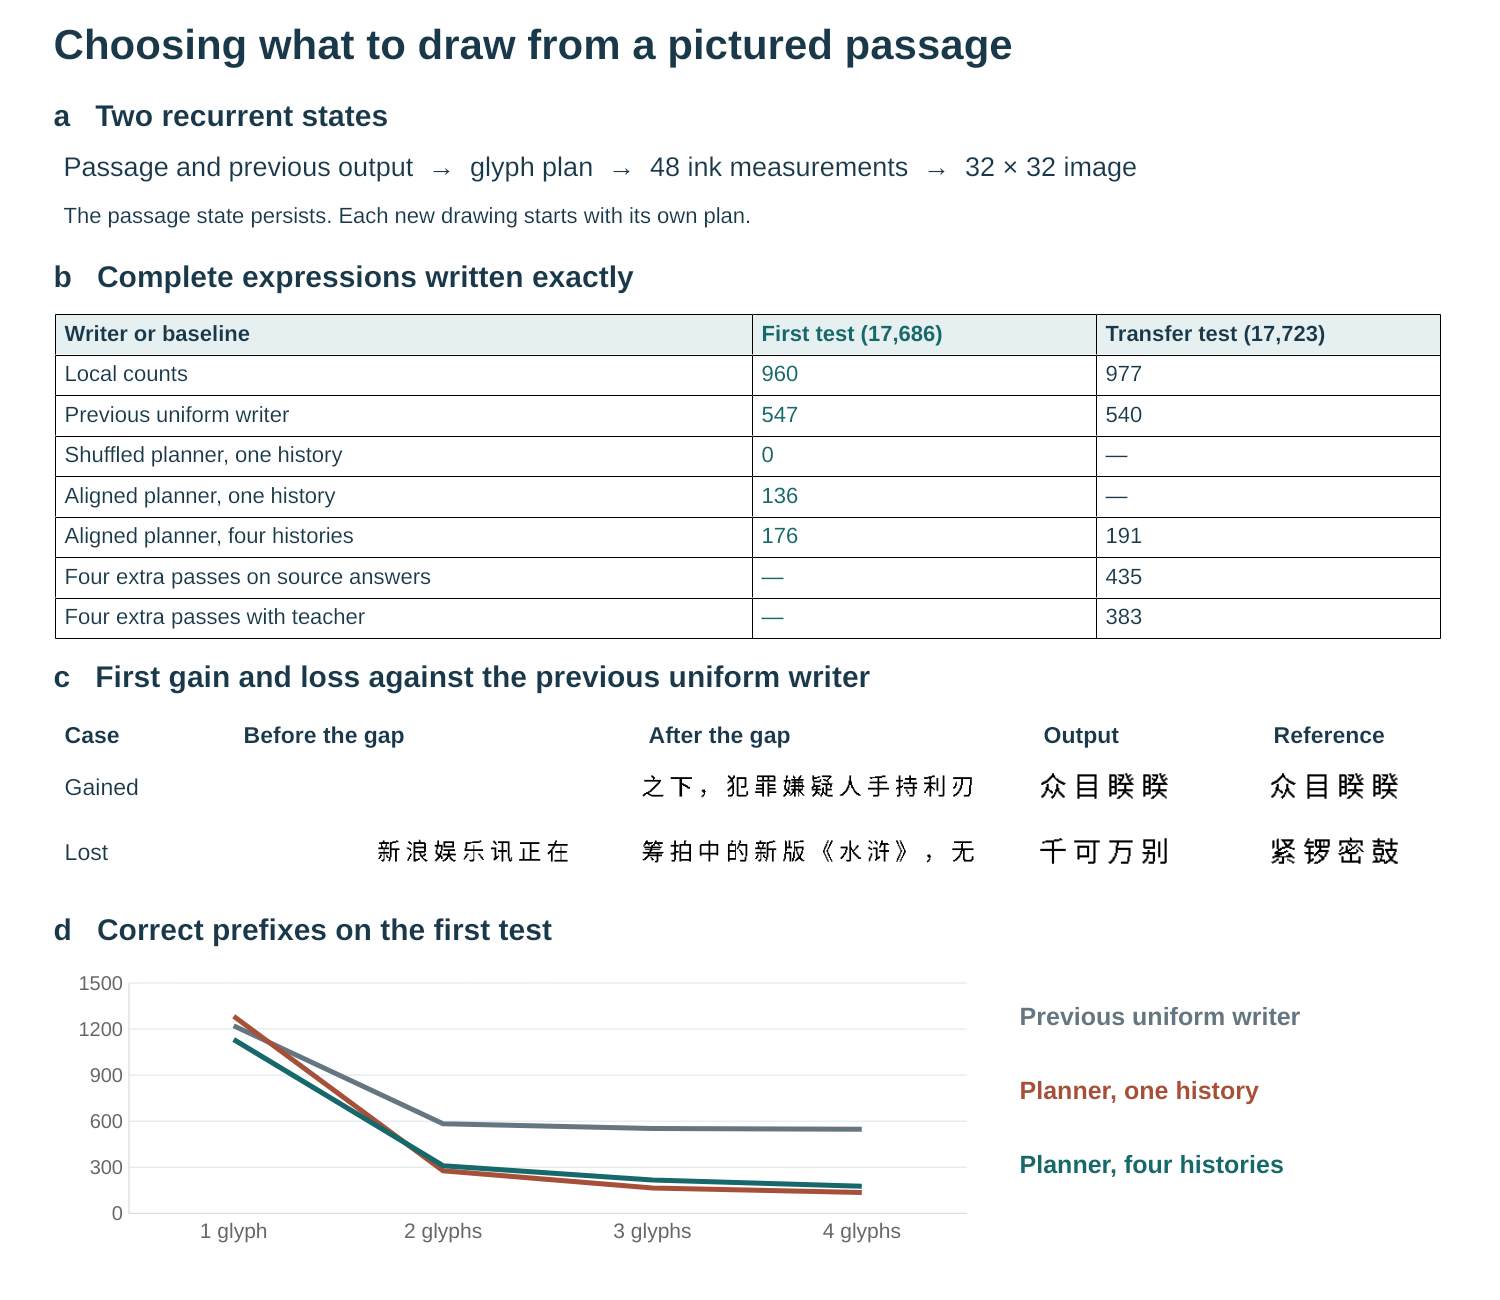
\includegraphics[width=.84\textwidth]{figures/Figure_46_glyph_planner.png}
\caption{\DIFaddFL{\textbf{Generating a missing expression with separate language and drawing states.}
\textbf{a}, Each arriving tile updates the passage-dependent state through measurements of the actual ink. The physical drawing recurrence starts anew for each tile.
\textbf{b}, Complete stopped expressions on two disjoint groups of held-out passages. The additional fits in the second test start from the aligned planner. The dashes identify conditions outside that comparison.
\textbf{c}, Original emitted pixels in the first gain and loss in source order for the aligned planner with one answer history relative to the uniform writer.
\textbf{d}, Number of passages with an exact prefix through each glyph on the first test. The fourth point counts four exact glyphs. Each reported complete answer also stopped at four.}}
\label{fig:glyph-planner}
\end{figure*}
\begin{figure*}[p]
\centering
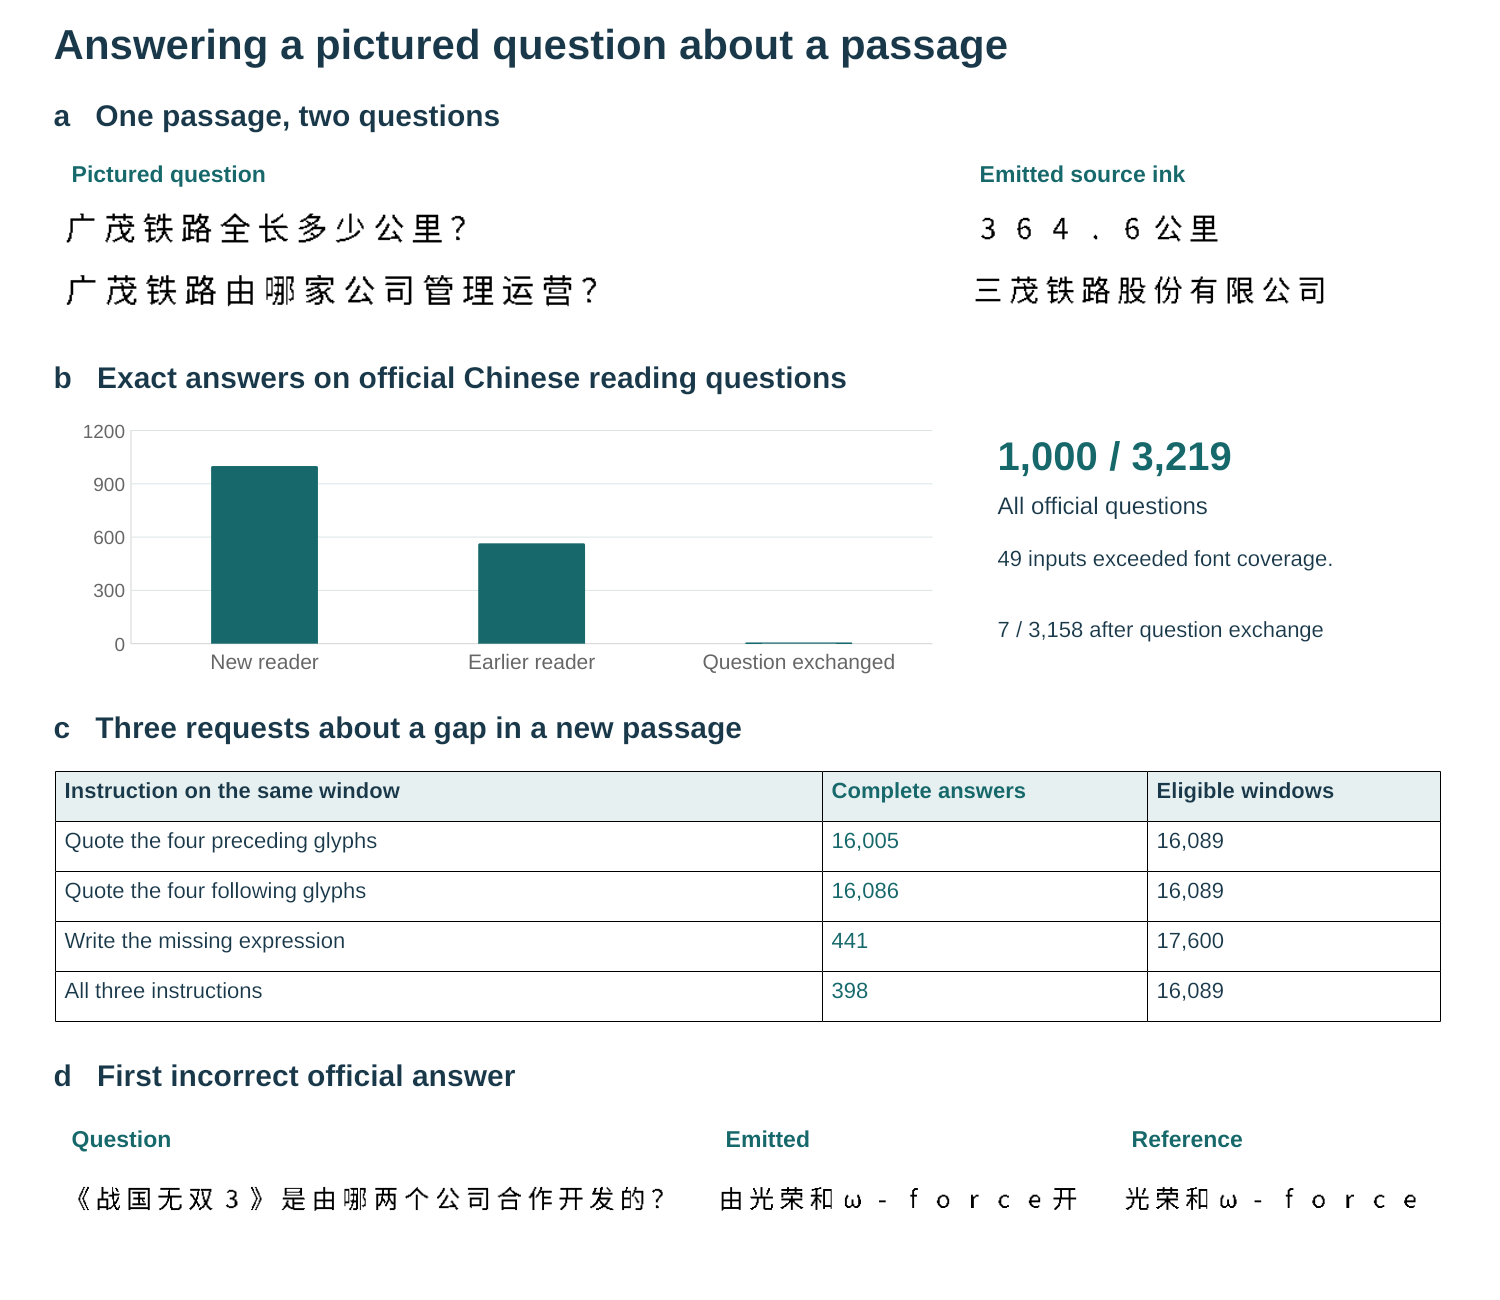
\includegraphics[width=.84\textwidth]{figures/Figure_47_mixed_ink.png}
\caption{\DIFaddFL{\textbf{Choosing between visible and missing writing.}
\textbf{a}, Original question and answer images for the first correctly answered pair with disjoint references in official source order. Both questions concern the same railway passage.
\textbf{b}, Complete outputs equal to at least one accepted answer. The two readers saw the same passages. The exchange control scores against the original question.
\textbf{c}, Unseen instruction phrasings on 17,600 additional idiom windows. Neighbour questions require four visible glyphs on either side of the central gap.
\textbf{d}, The first incorrect official output includes additional marks around the company names.}}
\label{fig:mixed-ink}
\end{figure*}
\begin{figure*}[p]
\centering
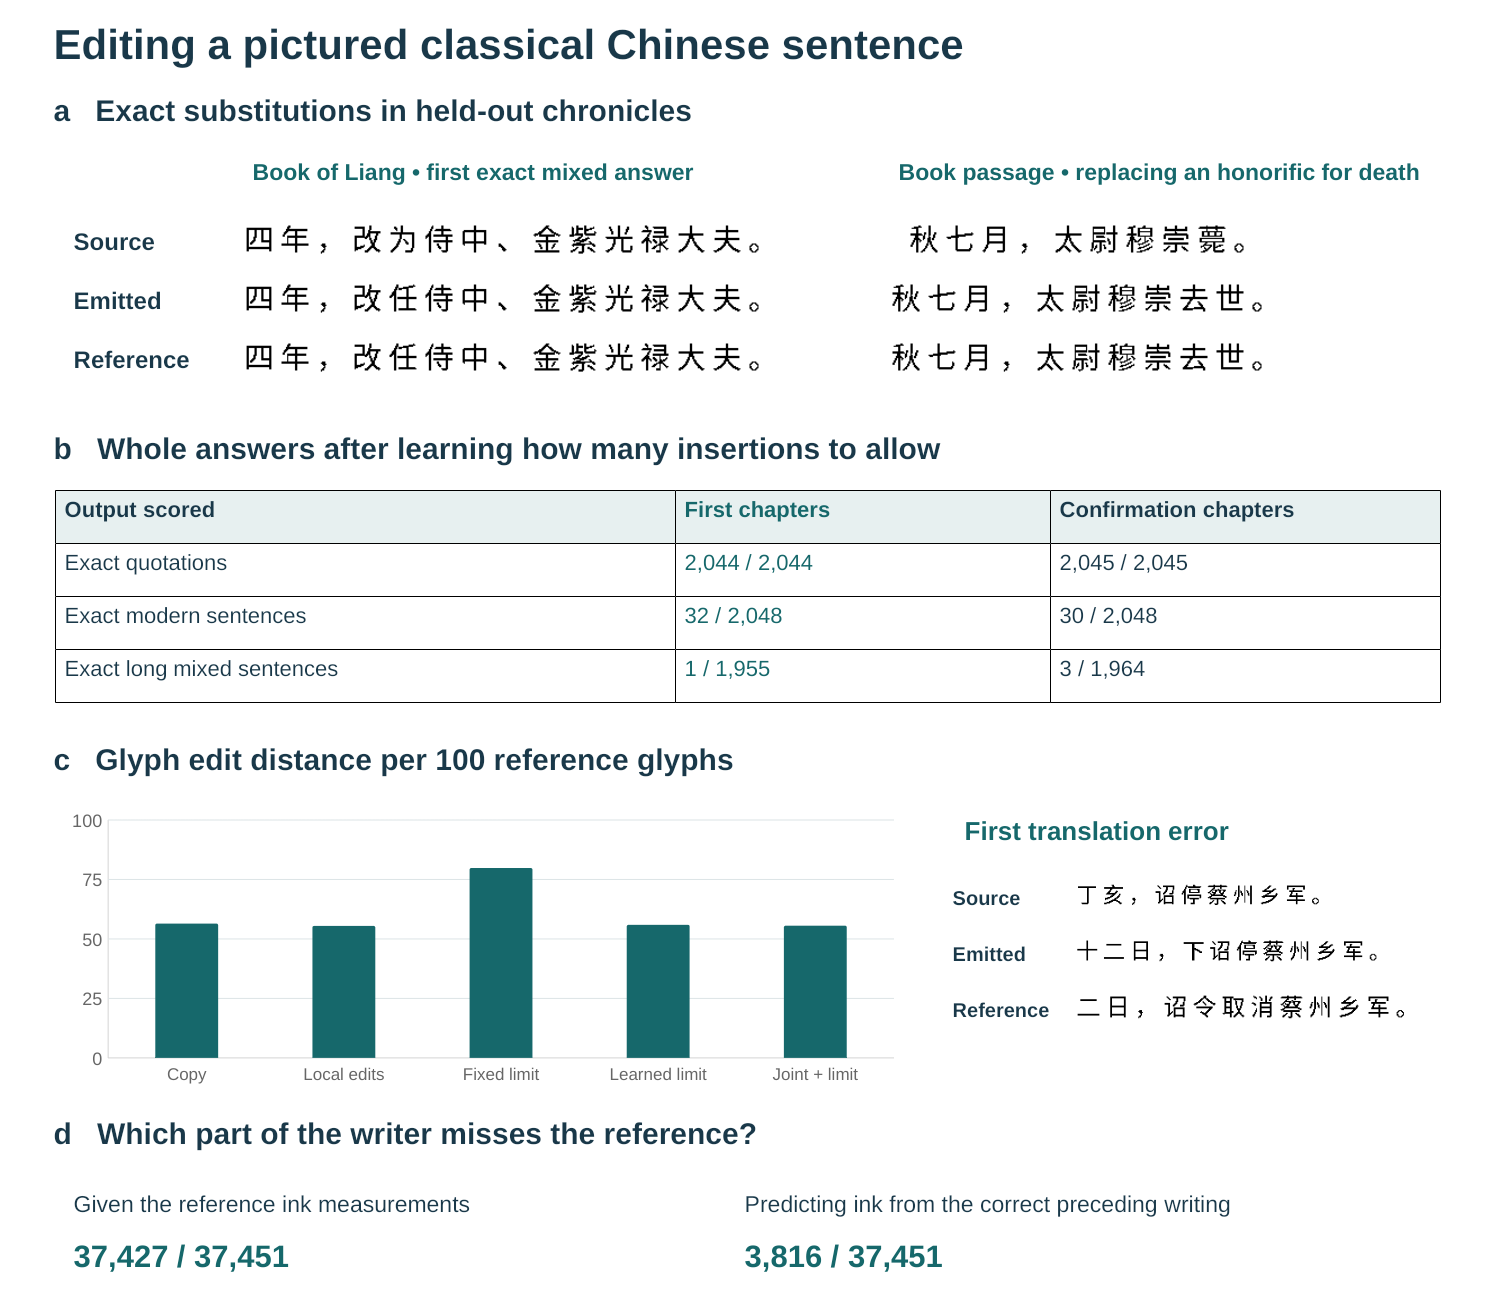
\includegraphics[width=.84\textwidth]{figures/Figure_48_visual_edit.png}
\caption{\DIFaddFL{\textbf{Copying and drawing within a sentence.}
\textbf{a}, Saved inputs, predictions and references from two confirmation chapters. The first exact mixed answer copies 14 glyphs and replaces one. The second example copies nine and draws two to express death in modern Chinese.
\textbf{b}, Whole stopped answers under the learned insertion limit. Mixed references exceed eight glyphs and contain both a source glyph and an absent Han character.
\textbf{c}, Physical edit distance on the first roster and the first failed translation in roster order. The local control learns edit counts from short source neighbourhoods.
\textbf{d}, Exact drawings with the recorded cursor and preceding ink. Both conditions use the same renderer.}}
\label{fig:visual-edit}
\end{figure*}
\begin{figure*}[p]
\centering
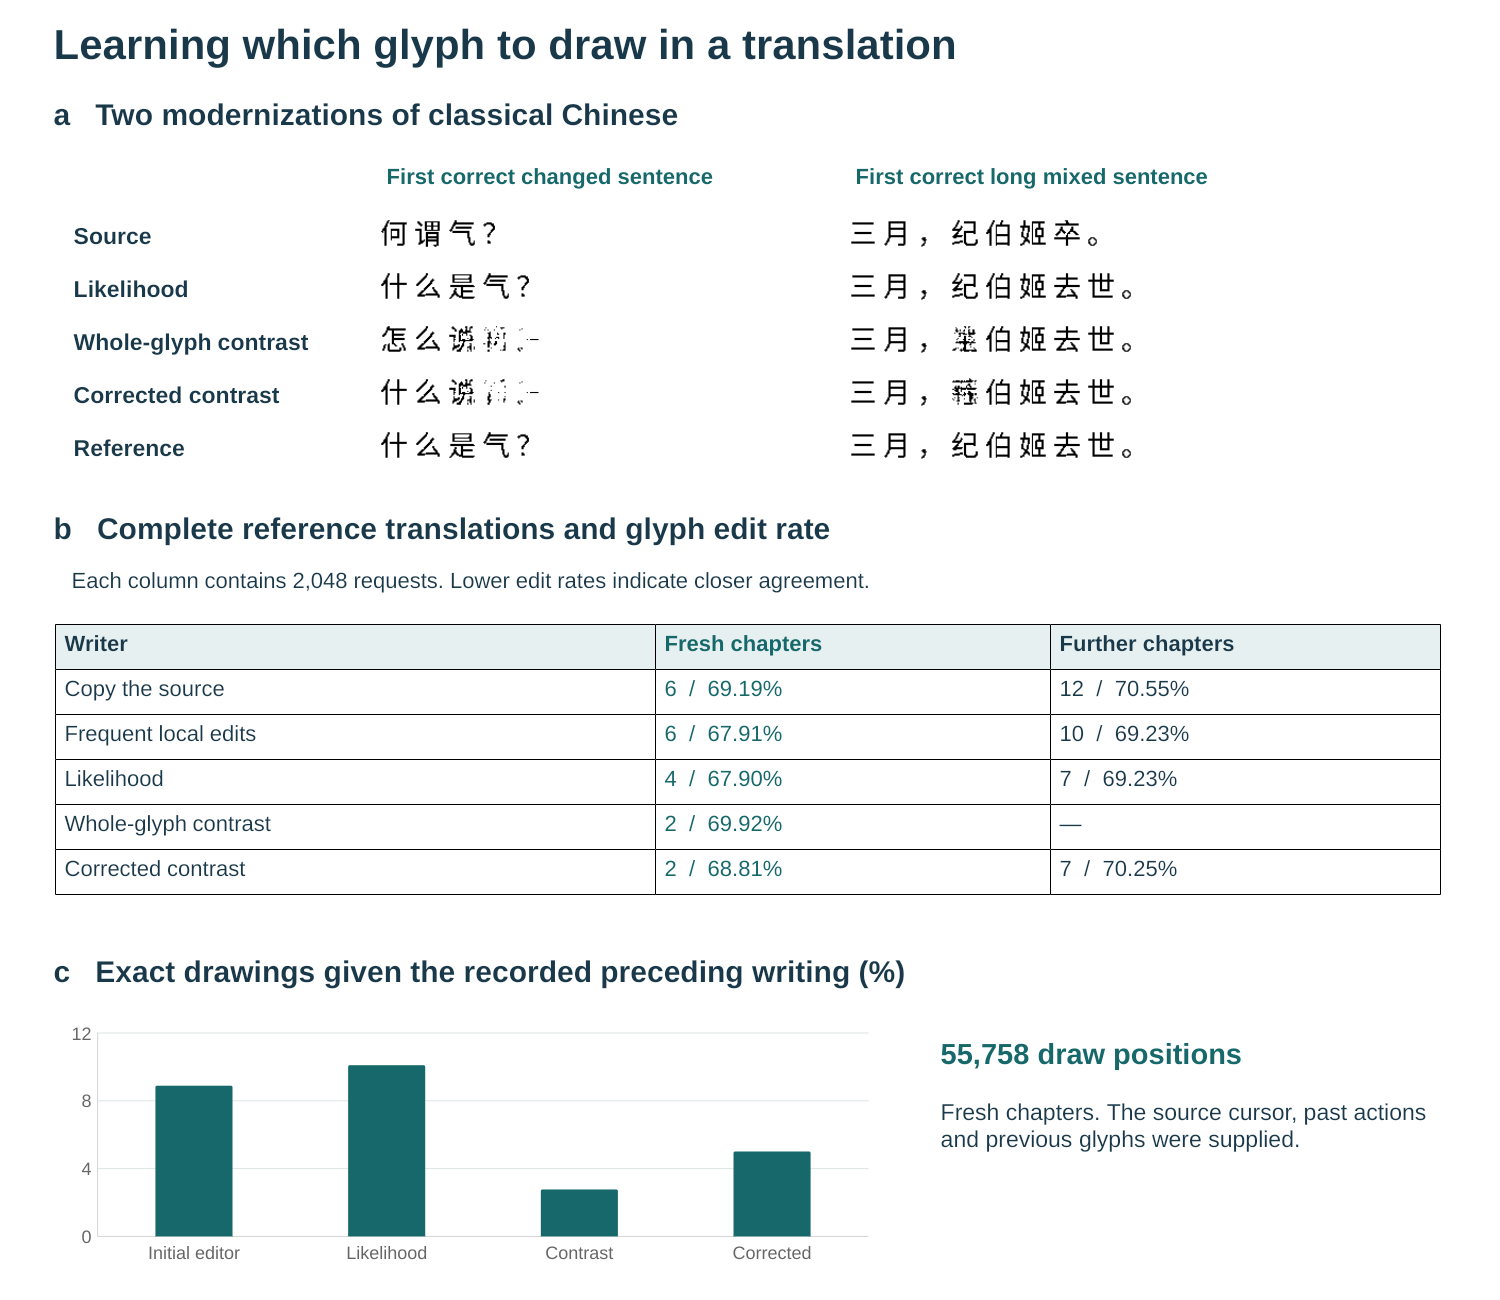
\includegraphics[width=.84\textwidth]{figures/Figure_49_edit_contrast.png}
\caption{\DIFaddFL{\textbf{Sentence editing with a complete-glyph training objective.}
\textbf{a}, Source, generated and reference pixels for the first changed sentence and the first longer mixed sentence that likelihood training reproduced exactly on the fresh chapters, in roster order. The instruction requests a modern Chinese translation.
\textbf{b}, Each entry gives the number of stopped translations exactly matching the reference image and aggregate glyph edit distance as a percentage of renderable reference length. Each roster contains 2,048 requests. The uncorrected contrast was evaluated on the first roster.
\textbf{c}, Exact emitted glyphs at recorded drawing positions on the first roster. The three additional fits share initial weights, sampled passages and number of updates.}}
\label{fig:edit-contrast}
\end{figure*}
\begin{figure*}[p]
\centering
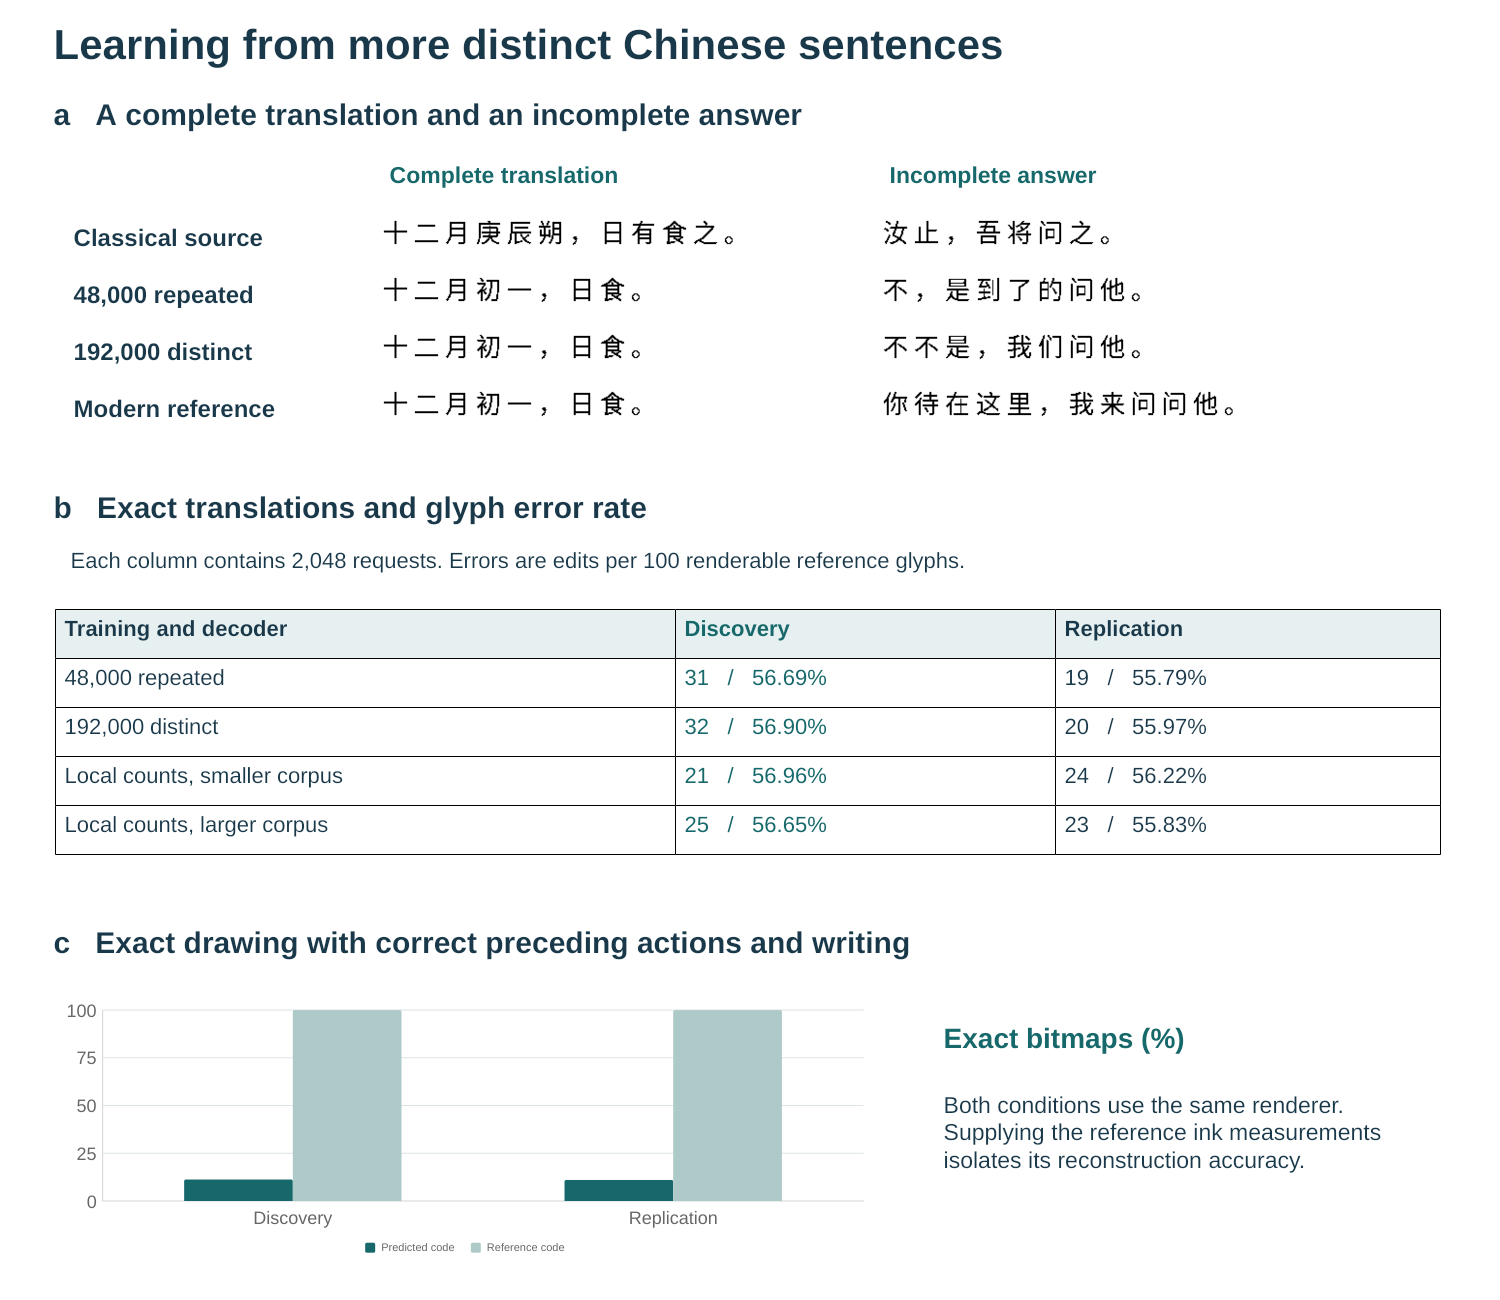
\includegraphics[width=.84\textwidth]{figures/Figure_50_edit_diversity.png}
\caption{\DIFaddFL{\textbf{Sentence diversity at equal training exposures.}
\textbf{a}, Actual glyph streams from the first exact discovery translation longer than eight cells with both shared and source-absent Han, and the first incorrect answer fitting fourteen cells. Both editors start from a common checkpoint. The labels give the number of distinct additional training pairs.
\textbf{b}, Exact stopped translations per 2,048 requests and total edits per 100 renderable reference cells. Each local rule uses the same unique pairs as its corresponding neural editor.
\textbf{c}, Exact 32-by-32 drawings at 39,435 and 37,543 recorded drawing positions. The darker bars use the larger-corpus editor's predicted physical code given correct prior writing. The lighter bars supply the reference code to its frozen renderer.}}
\label{fig:edit-diversity}
\end{figure*}
\begin{figure*}[p]
\centering
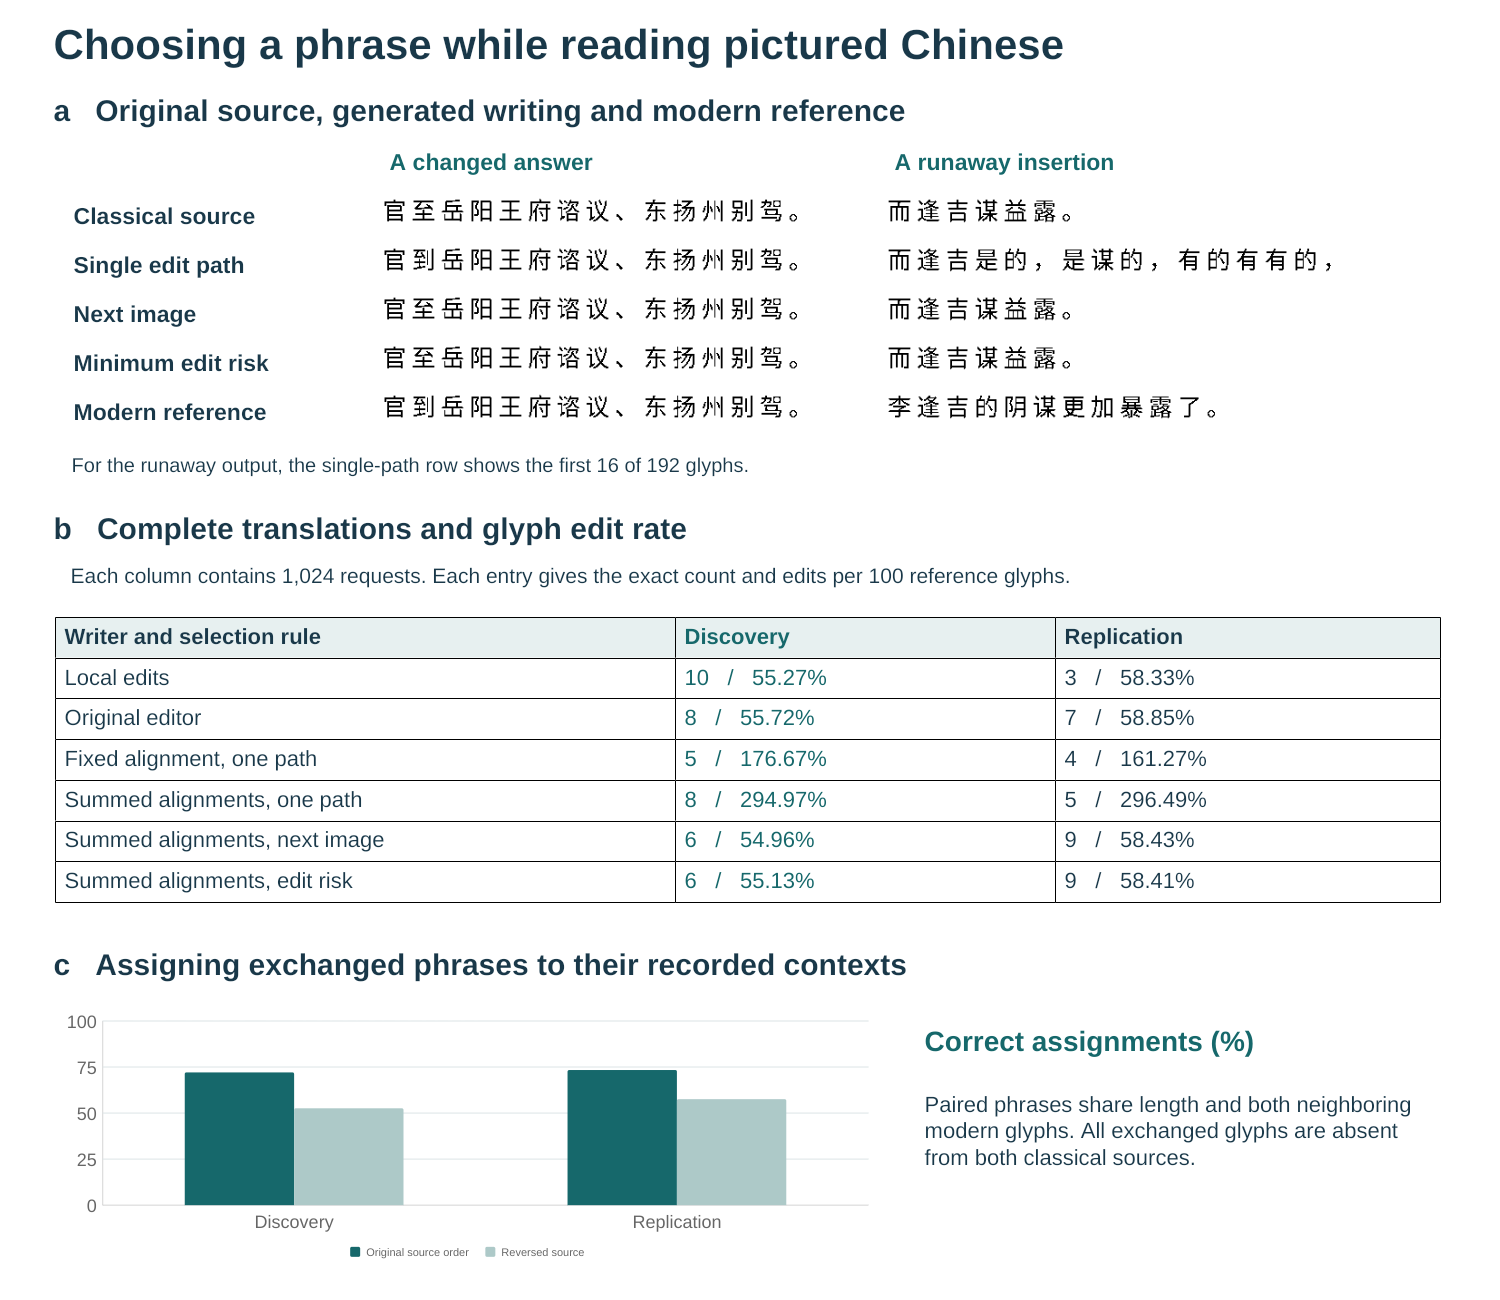
\includegraphics[width=.84\textwidth]{figures/Figure_51_visual_span.png}
\caption{\DIFaddFL{\textbf{Latent edit alignment in pictured translation.}
\textbf{a}, Actual generated pixels from the summed-alignment writer. The left example is its first exact discovery translation longer than eight cells that contains a source-absent Han glyph and shared writing. The right is the first capped translation with source and reference of at most fourteen glyphs. The single-path row in that column shows its first sixteen glyphs.
\textbf{b}, Exact translations per 1,024 requests and aggregate bitmap edit distance per 100 renderable reference glyphs. Next-image decoding sums compatible cursors for each emitted physical code. Minimum-risk selection uses separate samples to propose and score complete outputs.
\textbf{c}, Correct joint assignments of two natural inserted phrases using complete sentence probabilities. The phrases share length and immediate modern neighbors. Each has one to four glyphs, all absent from both sources. Reversal preserves the source glyph multiset.}}
\label{fig:visual-span}
\end{figure*}
\begin{figure*}[p]
\centering
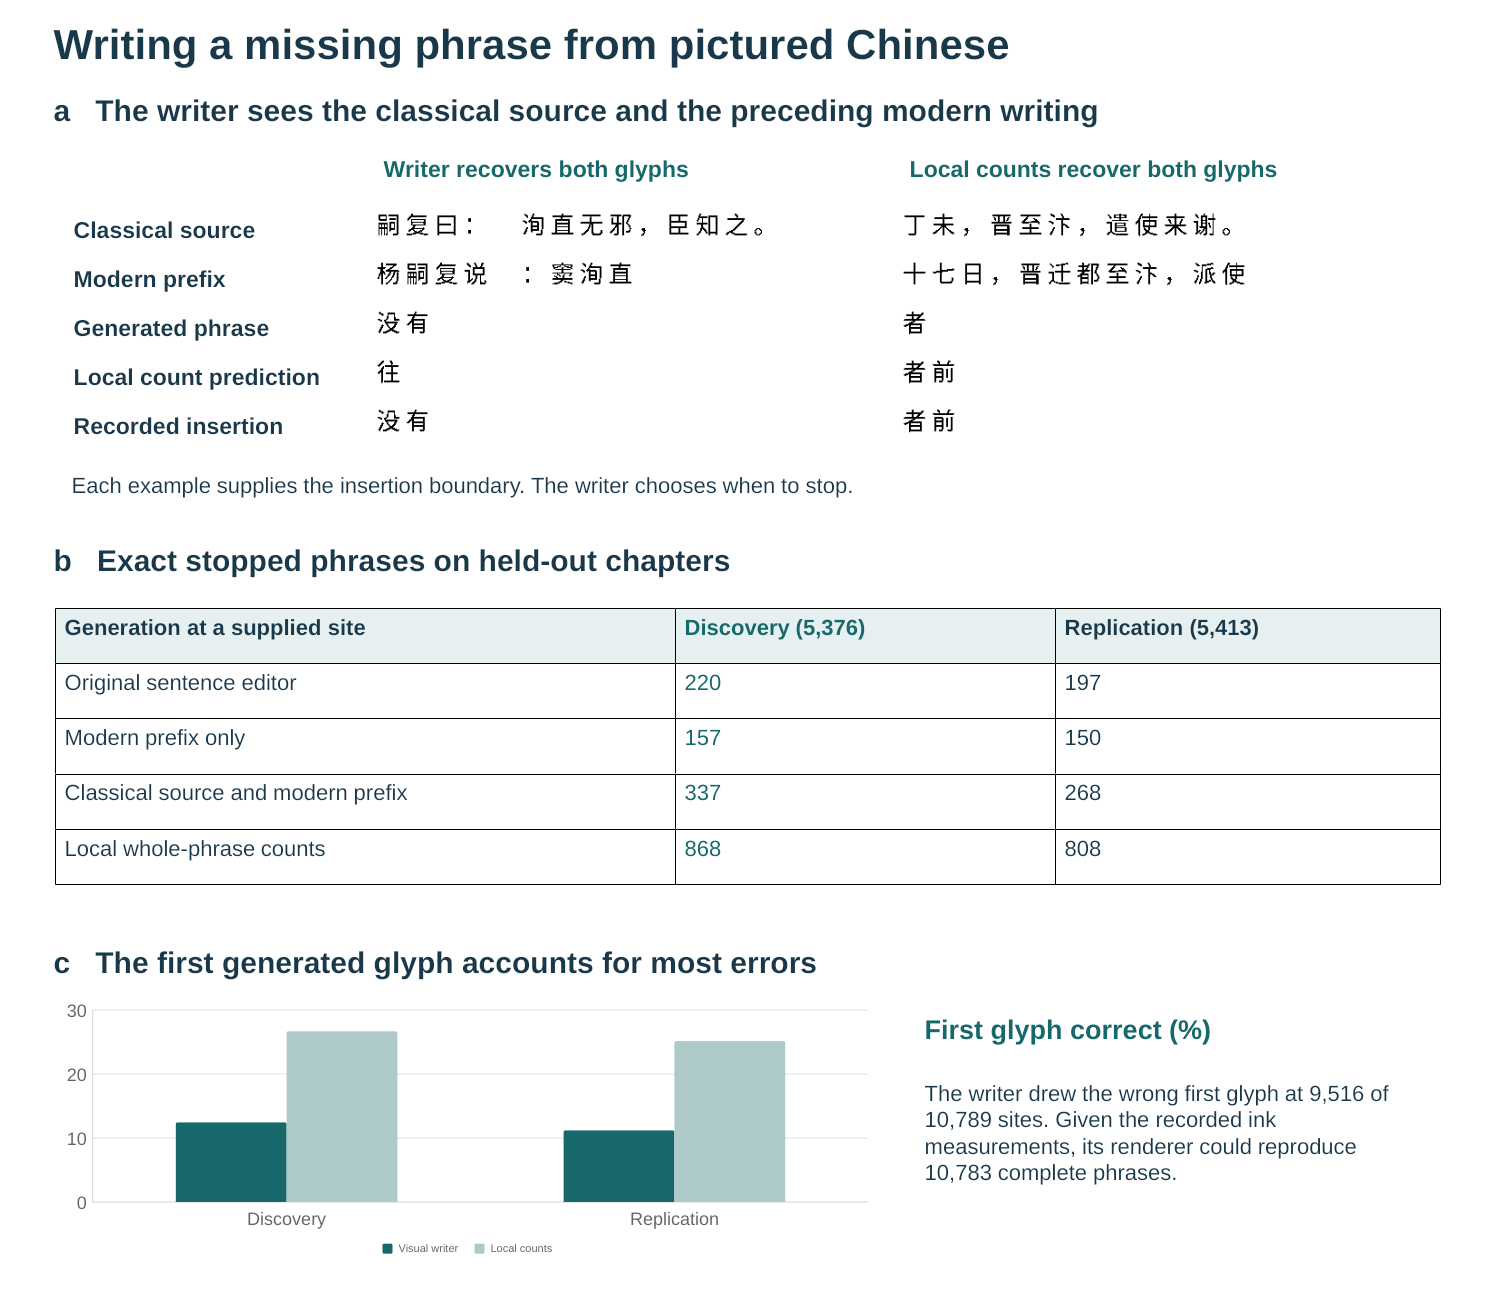
\includegraphics[width=.84\textwidth]{figures/Figure_52_visual_phrase.png}
\caption{\DIFaddFL{\textbf{Writing a modern phrase at a supplied insertion site.}
\textbf{a}, Original input, generated and reference images for two discovery examples. Both targets comprise two glyphs absent from the classical source. Each column uses the first qualifying example in roster order with a nonempty prefix and within the display bounds. The classical boundary falls after the seventh and ninth source cells, respectively.
\textbf{b}, Exact complete physical phrases including termination. The original editor is required to begin drawing at the same supplied site. Local counts select a whole phrase observed in training.
\textbf{c}, First-glyph identity. The neural writer can select between offered phrases using source order, but an error on its first independent glyph already prevents most recorded completions.}}
\label{fig:visual-phrase}
\end{figure*}
\begin{figure*}[p]
\centering
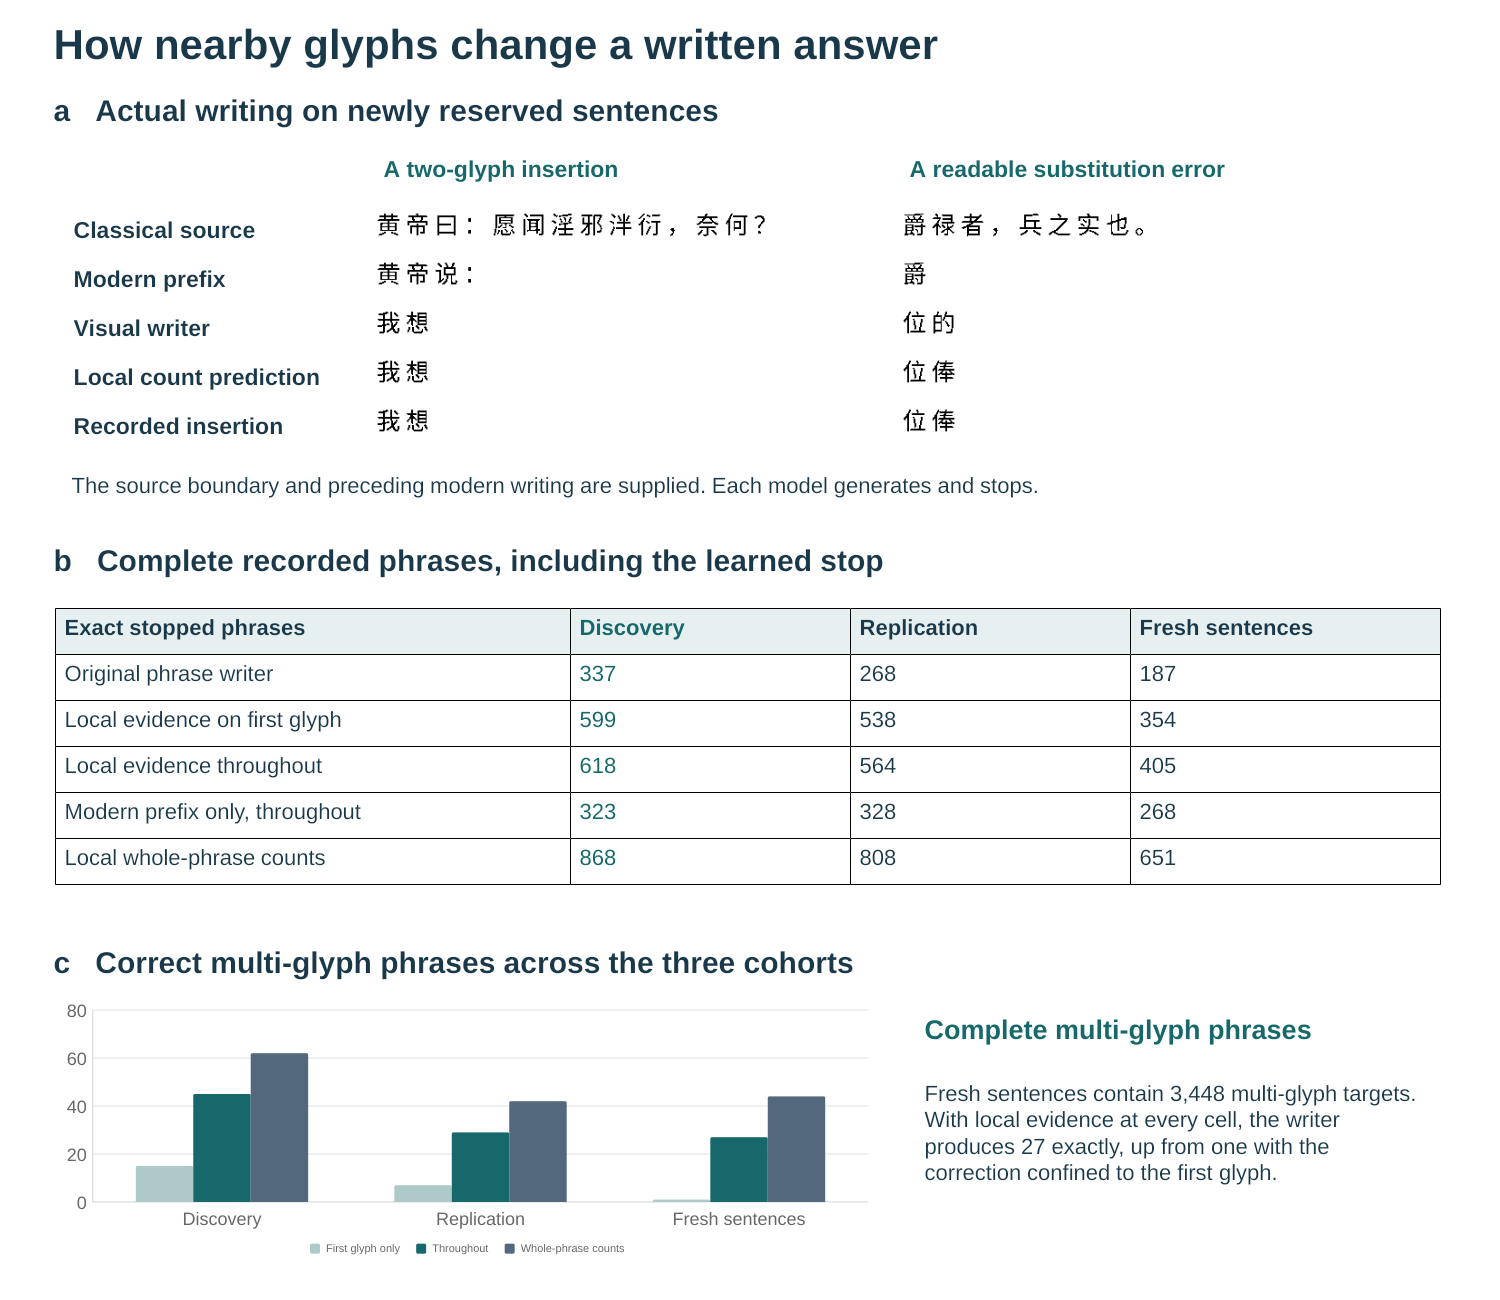
\includegraphics[width=.84\textwidth]{figures/Figure_53_local_ink.png}
\caption{\DIFaddFL{\textbf{Conditional visual frequencies in a Chinese phrase writer.}
\textbf{a}, Original source, modern prefix and emitted pixels from fresh sentences. Both recorded insertions have two characters absent from the source. On the left the writer produces the recorded first-person opening. On the right it produces a readable but incorrect second character. Examples were selected in roster order with a nonempty prefix and fixed display bounds. The respective boundaries follow the fourth and first source cells.
\textbf{b}, Exact stopped phrases in 5,376 discovery, 5,413 replication and 5,987 fresh sites. \textbf{c}, Multi-glyph completions out of 2,534, 2,679 and 3,448 targets. Both drawing corrections use the same frozen neural writer. The training-frequency rule selects complete observed phrases.}}
\label{fig:local-ink}
\end{figure*}
\begin{figure*}[p]
\centering
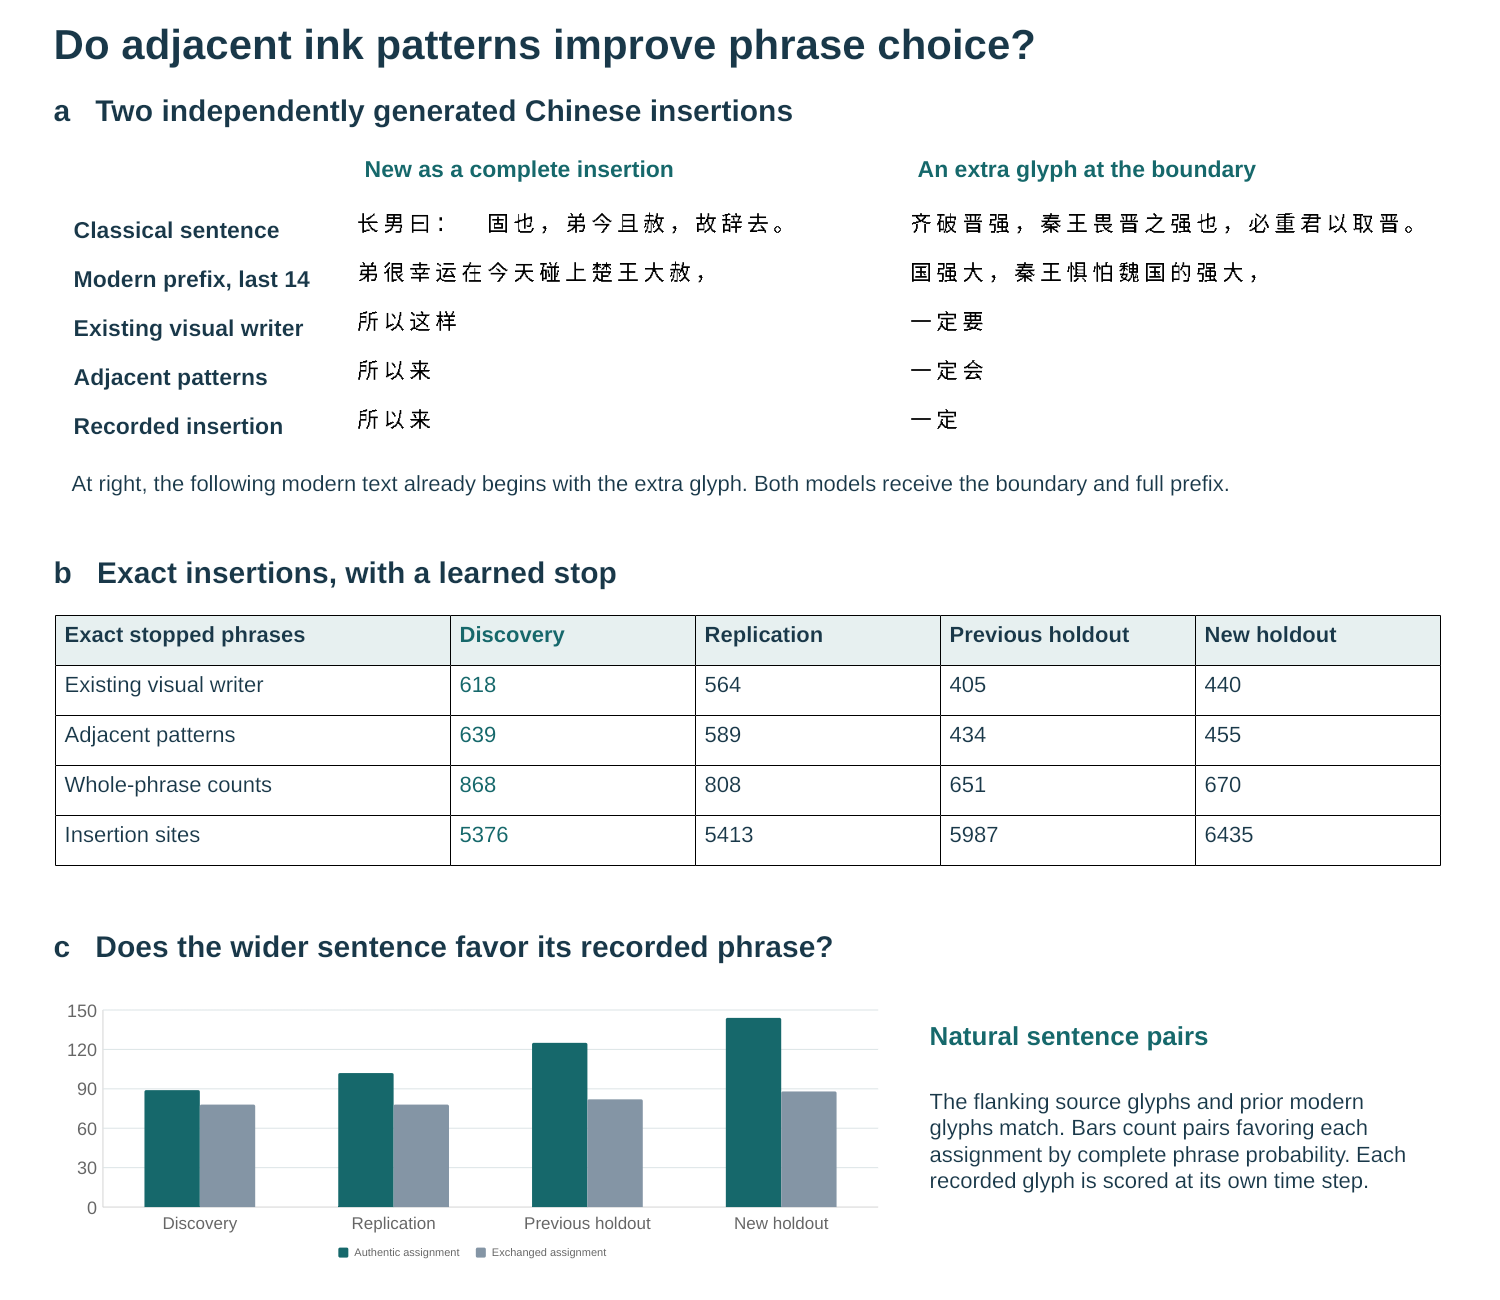
\includegraphics[width=.84\textwidth]{figures/Figure_54_conditional_ink_aligned.png}
\caption{\DIFaddFL{\textbf{Learning adjacent stroke patterns in Chinese phrase generation.}
\textbf{a}, Original images from the scored streams. At left the writer draws a three-glyph phrase absent as a complete insertion from its training inventory. The same sequence occurs in six modern training sentences. At right it draws an additional glyph already present at the start of the subsequent translation. Full modern prefixes and the classical source boundaries after cell 13 in each sentence are supplied; only the final 14 prefix cells are shown. The two examples come from the preceding and new holdouts respectively.
\textbf{b}, Exact stopped phrases at all aligned sites. The frequency control can choose complete observed phrases. \textbf{c}, Number of matched sentence pairs favoring each assignment of distinct source contexts to recorded insertions. Bars use the summed conditional log probability of both phrases including learned endings. The corrected chart aligns every drawing and ending score to its own target position.}}
\label{fig:conditional-ink}
\end{figure*}
\begin{figure*}[p]
\centering
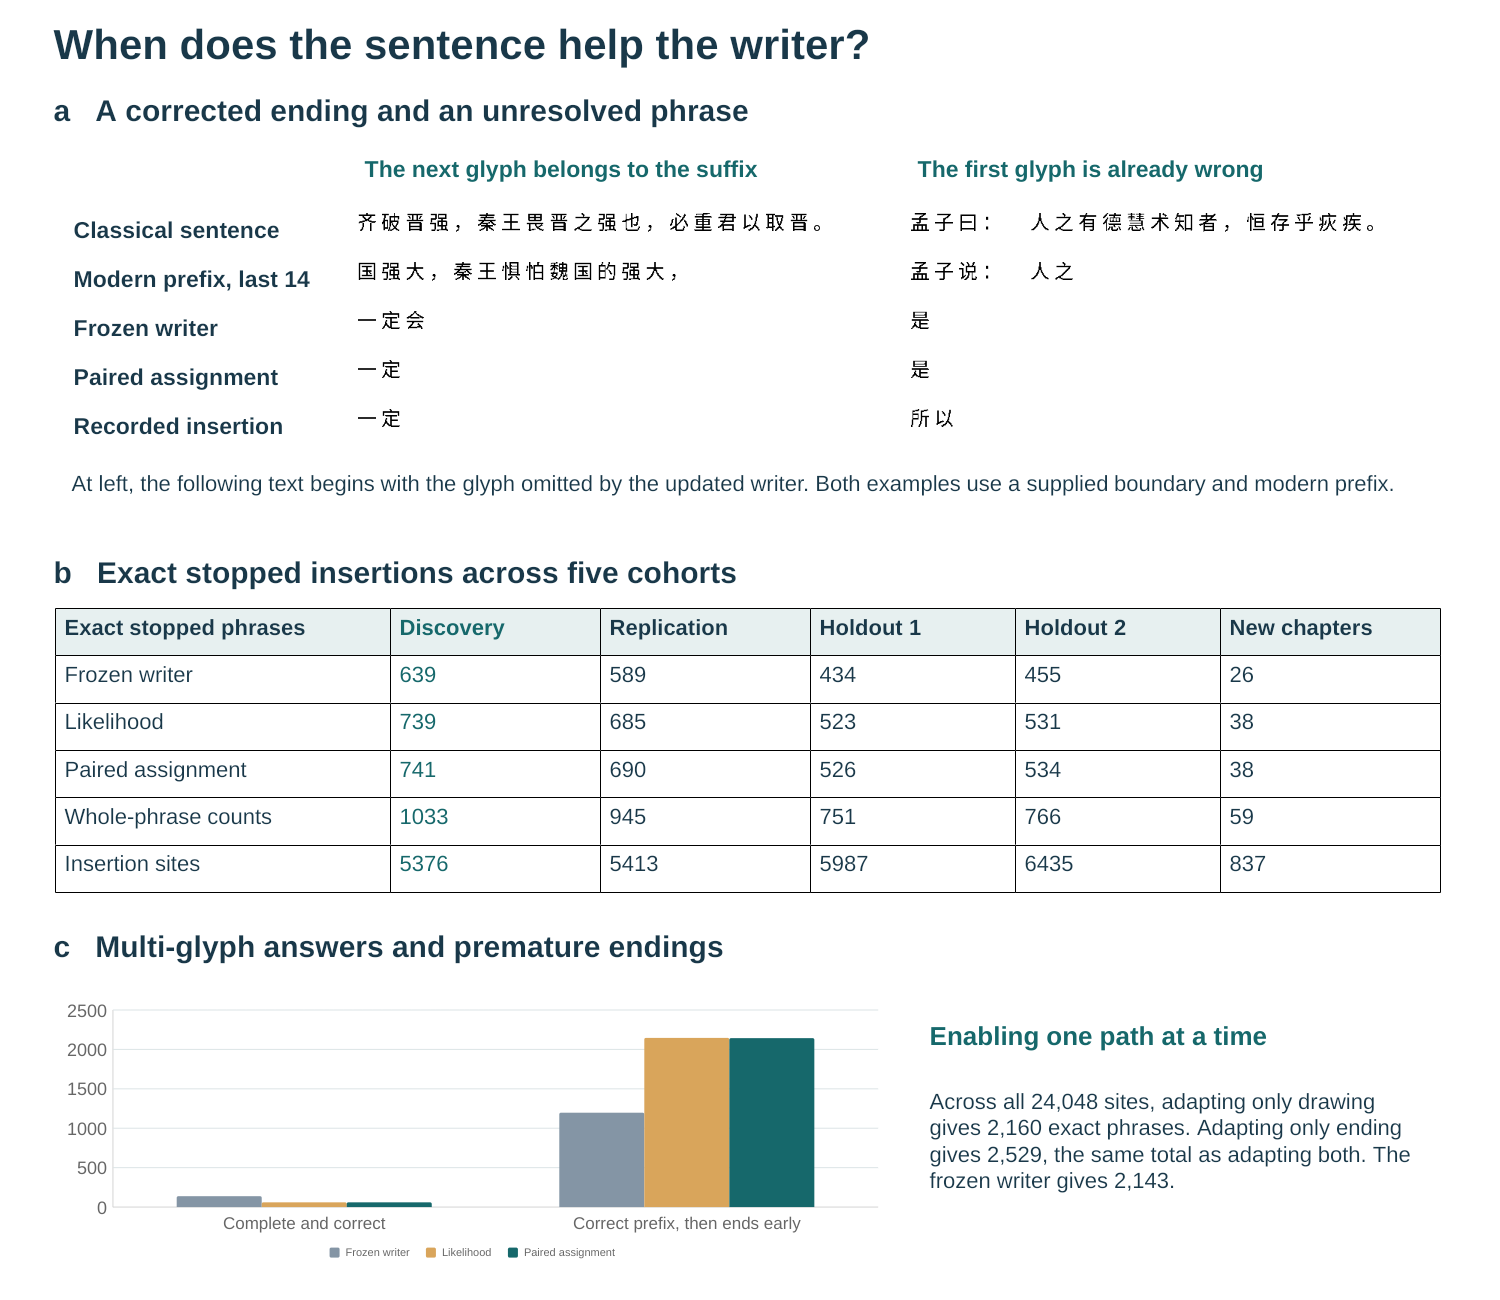
\includegraphics[width=.84\textwidth]{figures/Figure_55_sentence_choice.png}
\caption{\DIFaddFL{\textbf{Training on matched source sentences chiefly changes phrase endings.}
\textbf{a}, Original answer images from the second holdout. At left the updated model stops before a glyph already present in the following translation. At right both models draw the wrong first glyph. These are the first qualifying bounded multi-glyph gain over the frozen writer and error solved by whole-phrase counts, in roster order. The insertion boundary is supplied after source cells 13 and 7, respectively.
\textbf{b}, Exact full image sequences with an autonomous stop. The final column includes all 84 remaining eligible classical sentences across 75 chapters. \textbf{c}, Complete successes and strictly shorter correct prefixes on 13,041 multi-glyph targets. Path-specific counts in the adjacent text use all 24,048 insertion sites.}}
\label{fig:sentence-choice}
\end{figure*}
\begin{figure*}[p]
\centering
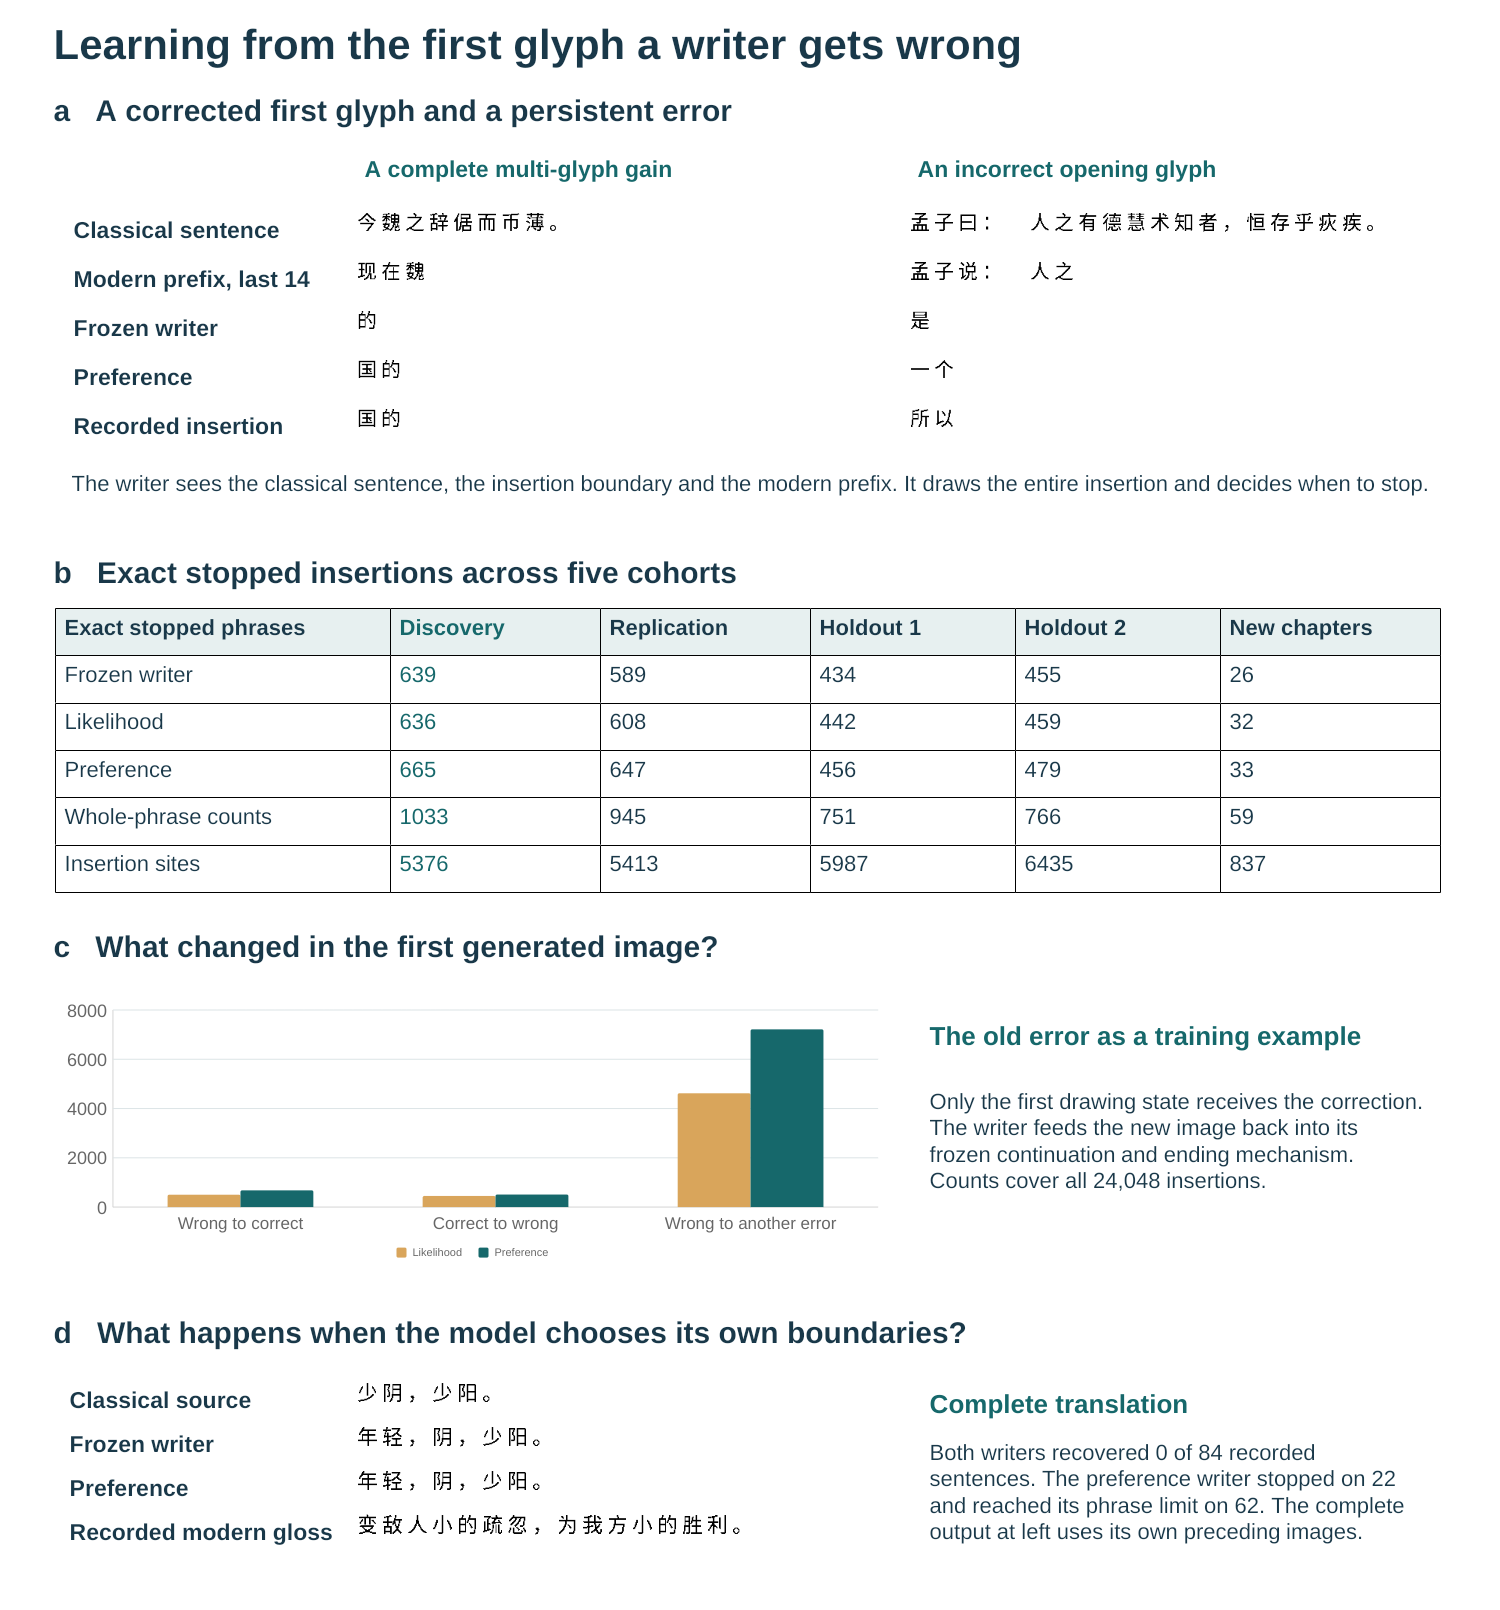
\includegraphics[width=.84\textwidth]{figures/Figure_56_first_emission.png}
\caption{\DIFaddFL{\textbf{First-glyph preference learning changes the content of Chinese insertions.}
\textbf{a}, Original bitmaps from the second holdout. The examples are the first bounded multi-glyph gain with a corrected first image and the first wrong first image for which the count model supplies the entire phrase, in source order. The supplied boundaries are after source cells 2 and 7, respectively. The writer receives the complete modern prefix. The final 14 cells fit in the panel.
\textbf{b}, Exact complete bitmap sequences with a learned stop at all enrolled sites. The enlarged count control uses complete observed insertions. \textbf{c}, Paired changes in the first emitted image relative to the frozen writer. A change to a different wrong image counts only when both emissions differ from the reference. Each bar compares original 32-by-32 bitmaps. \textbf{d}, Autonomous translation with the pictured source and instruction only. The first short case whose entire reference and both entire generated streams fit in 25 cells is shown. The modern gloss is specific to the source corpus.}}
\label{fig:first-emission}
\end{figure*}
\begin{figure*}[p]
\centering
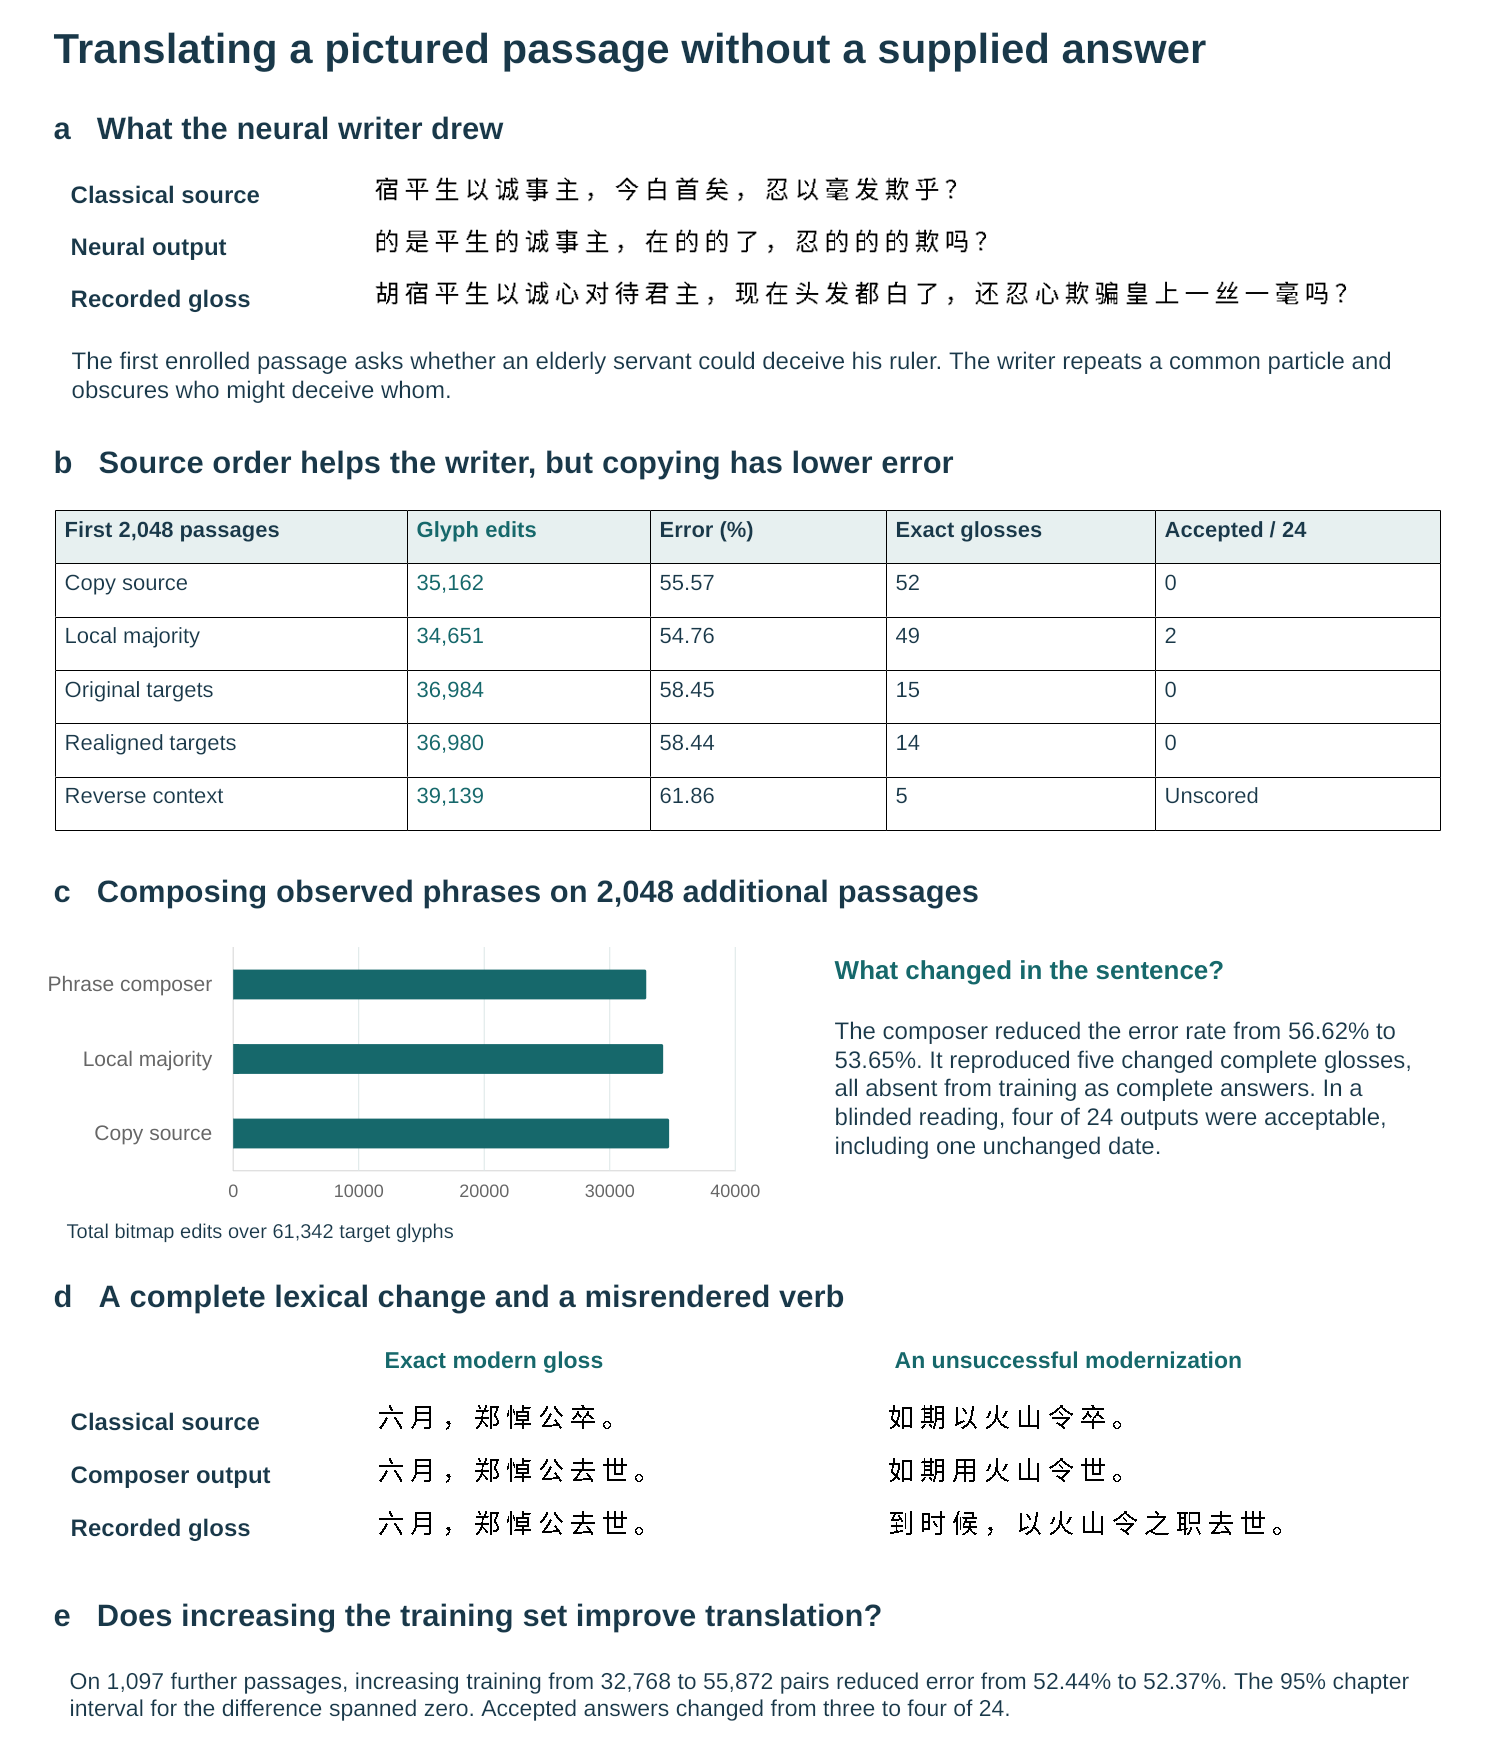
\includegraphics[width=.84\textwidth]{figures/Figure_57_block_translation.png}
\caption{\DIFaddFL{\textbf{Complete visual translation with the classical source alone.}
\textbf{a}, First enrolled passage, realigned neural output and corpus gloss, shown as their original 32-by-32 cells. The writer repeats a common particle in positions requiring different words. \textbf{b}, Complete physical edit distance and exact modern glosses in 2,048 passages with 63,274 reference cells. The reversed control presents the same glyphs in reverse to the encoder and restores the source positions before emission. Acceptance required a complete modern rendering in a separately blinded 24-passage reading. \textbf{c}, Total glyph edits in a second cohort of 2,048 passages. \textbf{d}, First changed exact composer output in cohort order and first erroneous composer output from the blinded reading with a reference of at most 16 cells. The left gloss changes the classical verb of death into its two-glyph modern equivalent. The right output fails on the same verb after an official title. \textbf{e}, Training size comparison on 1,097 previously unevaluated passages. The scoring rule and language weight are fixed. The larger model made 24 fewer glyph edits over 33,879 target cells.}}
\label{fig:block-translation}
\end{figure*}
\begin{figure*}[p]
\centering
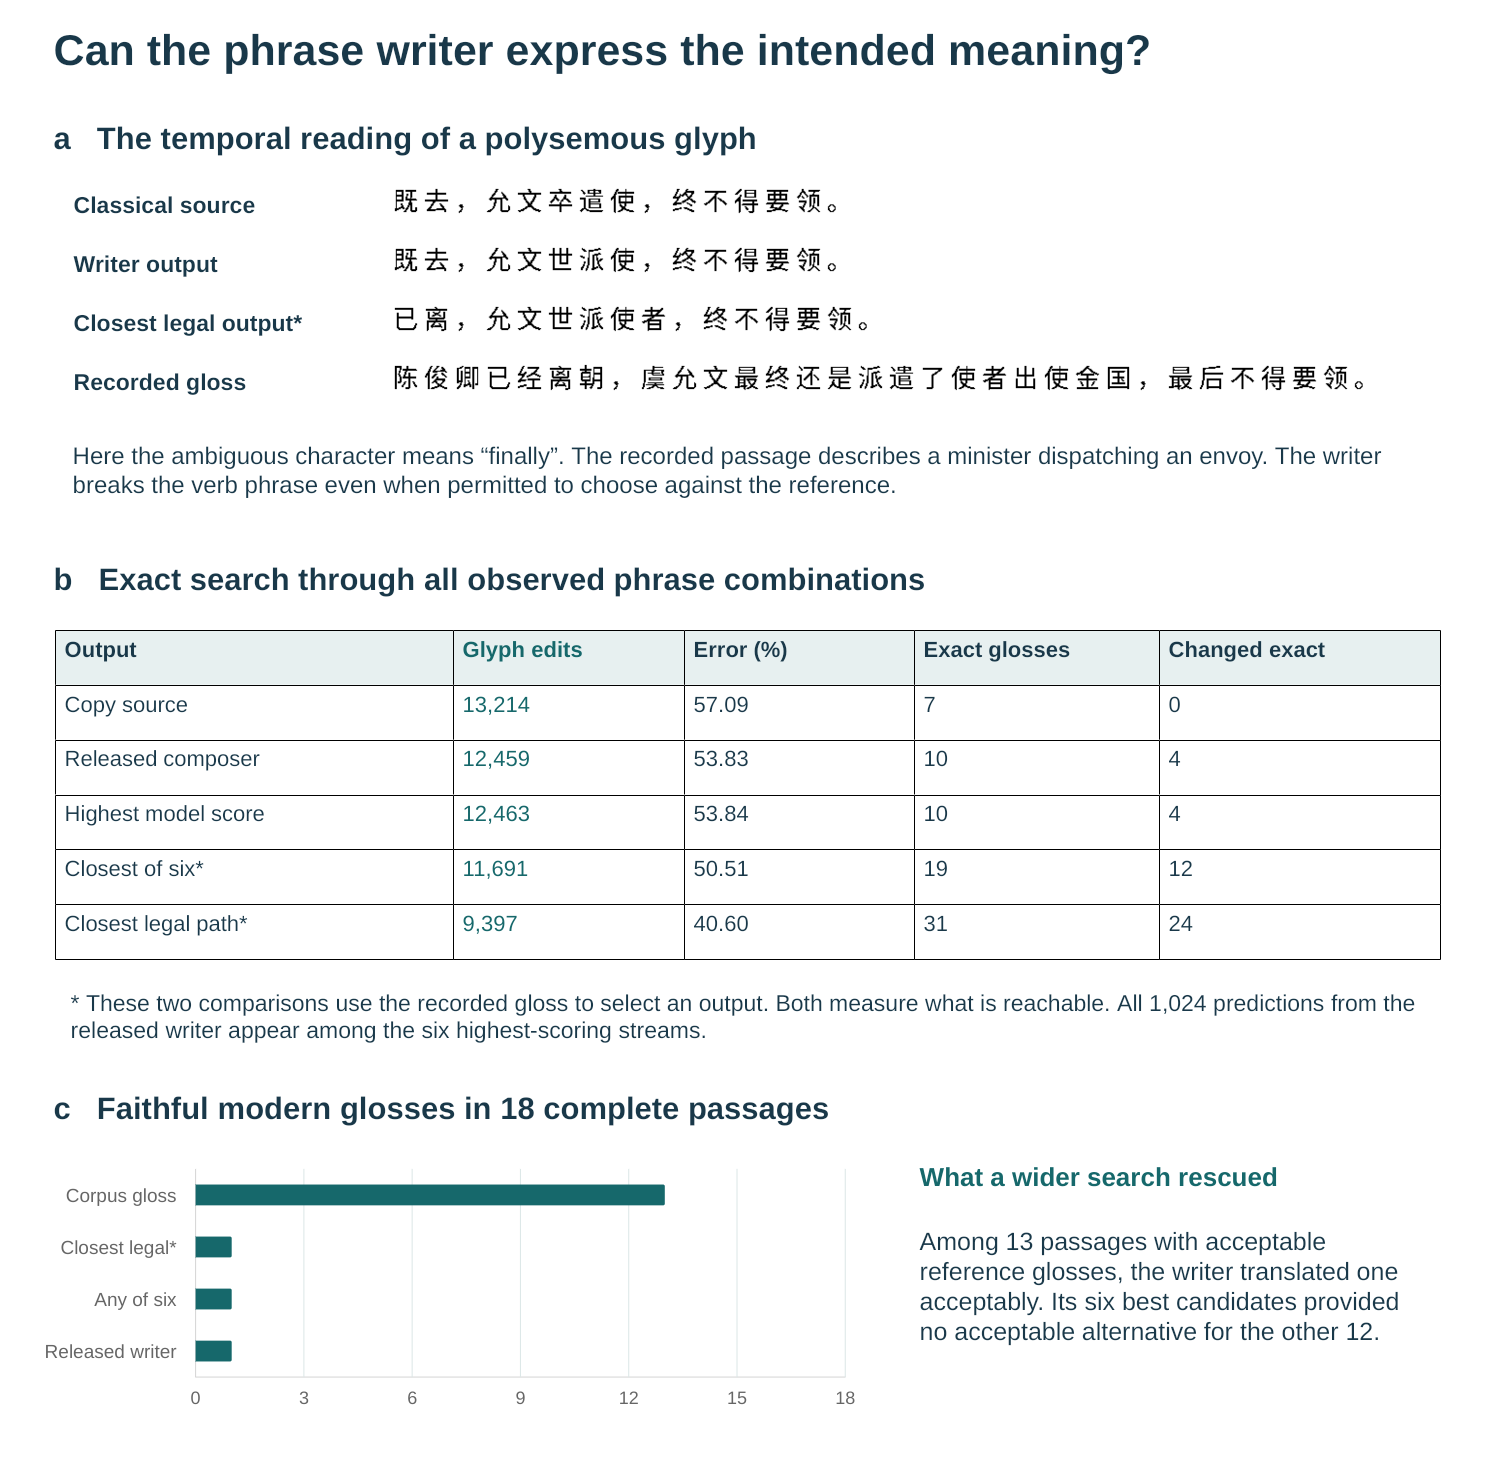
\includegraphics[width=.84\textwidth]{figures/Figure_58_clause_support.png}
\caption{\DIFaddFL{\textbf{Reachable glosses of a fixed visual phrase writer.} \textbf{a}, Original complete glyph strips for a temporal use of a polysemous character, with the recorded gloss and the legal output closest to it. \textbf{b}, Physical edit distance over 23,147 reference cells. The two starred rows use the reference to select a stream. An exact output need not require a change from the source. \textbf{c}, Number of complete, faithful modern renderings in eighteen passages graded with method assignments concealed. The widest answer-informed search minimizes bitmap edit distance. The reading of its witness remains a separate measurement.}}
\label{fig:clause-support}
\end{figure*}
\begin{figure*}[p]
\centering
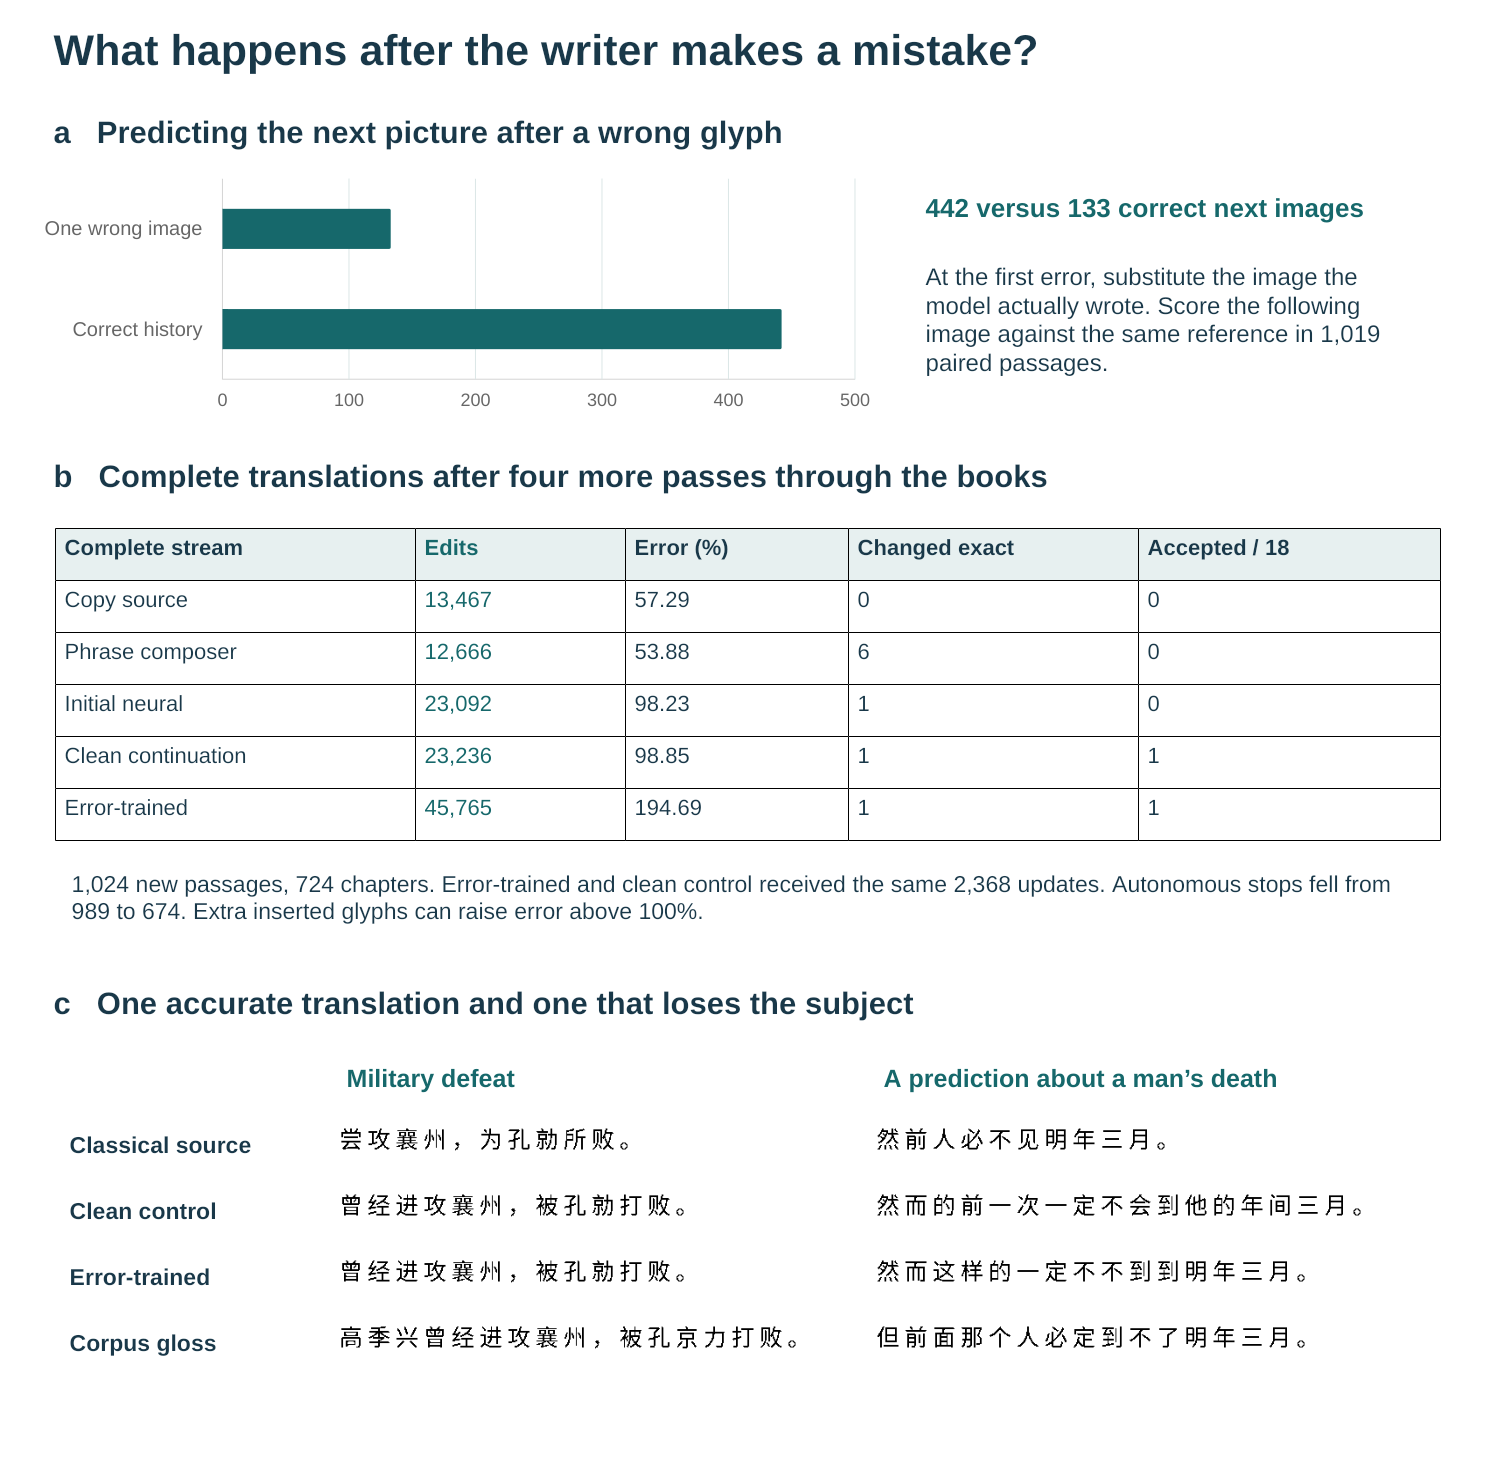
\includegraphics[width=.84\textwidth]{figures/Figure_59_visual_feedback.png}
\caption{\DIFaddFL{\textbf{Visual feedback during autonomous classical-to-modern translation.} \textbf{a}, Correct next-image predictions among 1,019 paired histories from the initial writer. Only the previous picture at the first observed error changes. \textbf{b}, Complete-stream scores on a new 1,024-passage evaluation. The two continuation arms begin from identical weights. Eighteen passages were read with method assignments concealed. \textbf{c}, Full, unretouched output pixels for the sole accepted error-trained answer and the first unaccepted answer with a faithful reference and all four strips at most twenty cells long. In the first corpus gloss a personal-name character is printed as two components. Both models preserve the proper name in that answer. In the second they lose who is predicted to die.}}
\label{fig:visual-feedback}
\end{figure*}
\begin{figure*}[p]
\centering
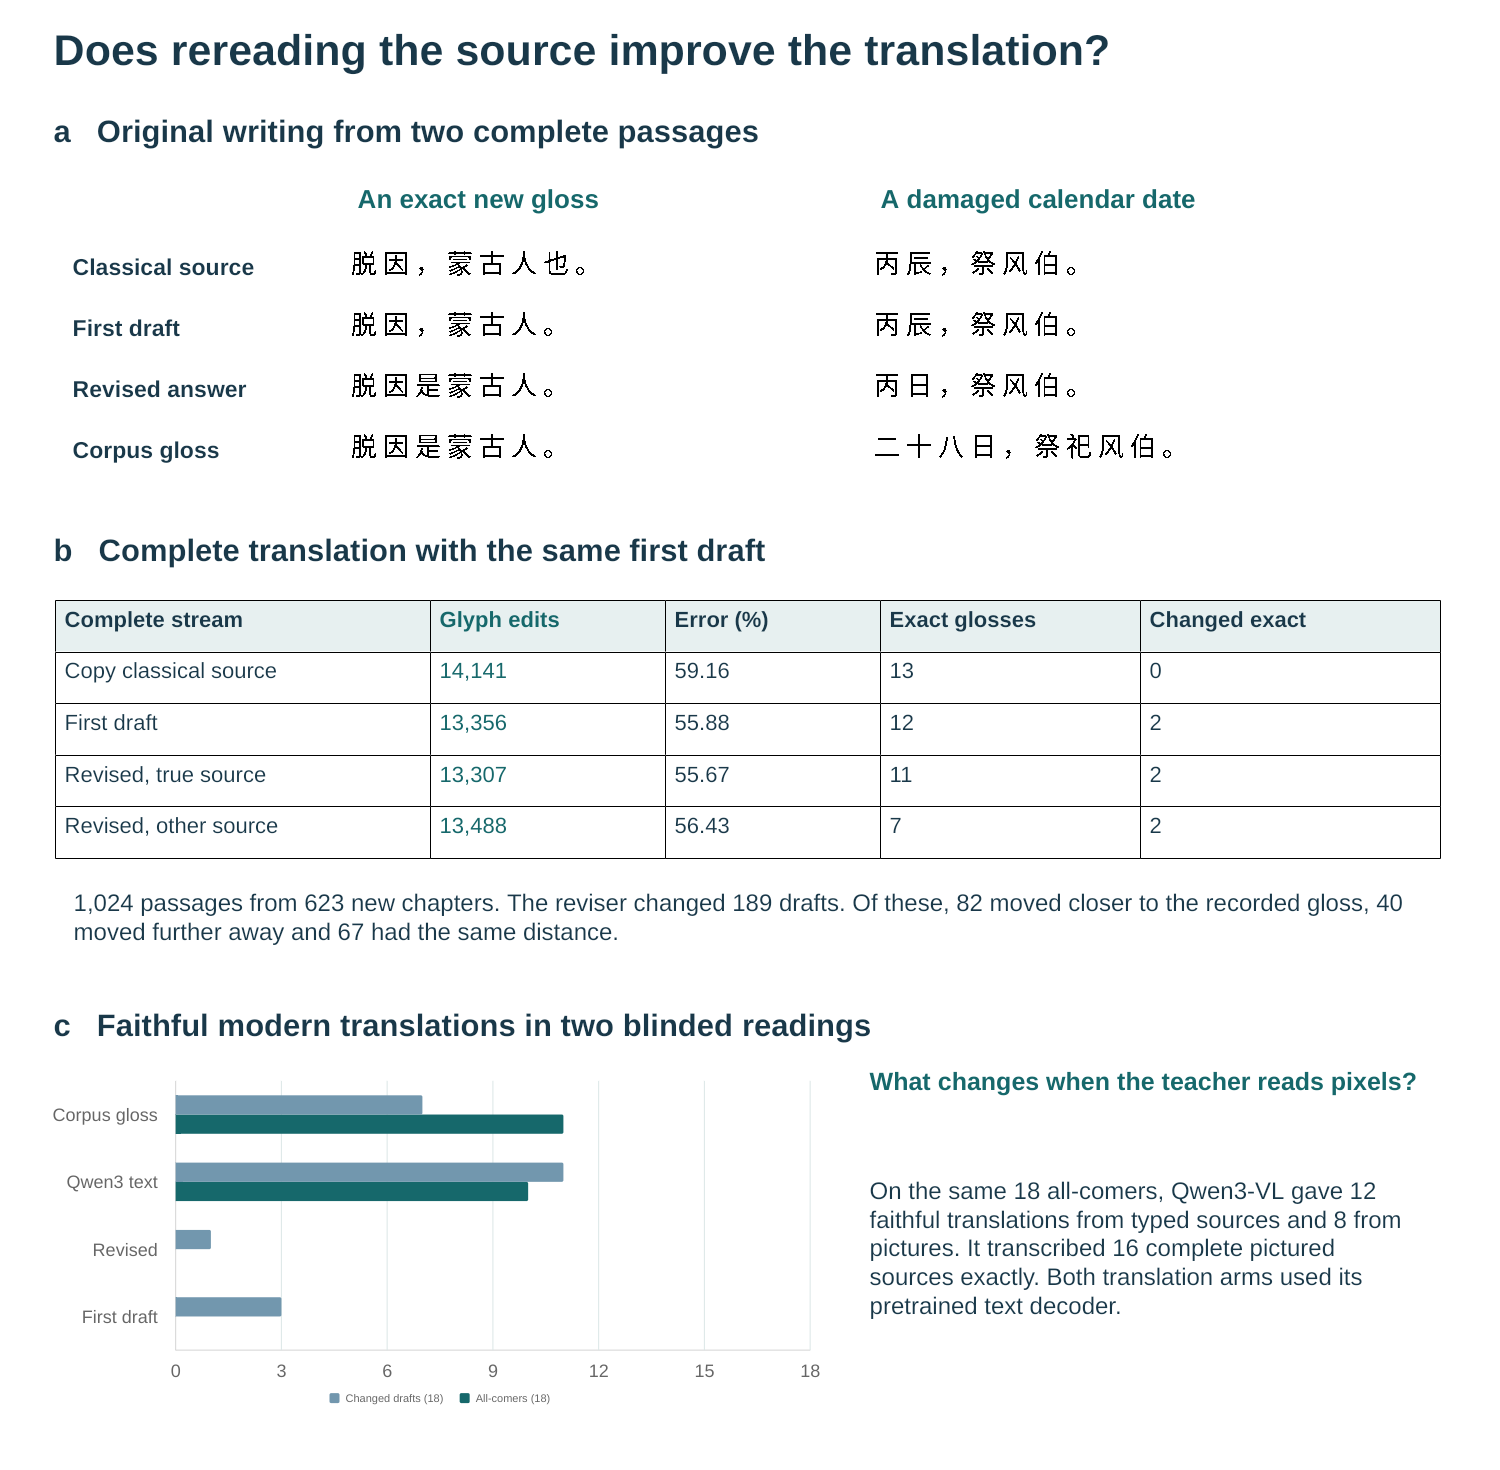
\includegraphics[width=.84\textwidth]{figures/Figure_60_pictured_revision.png}
\caption{\DIFaddFL{\textbf{A source-conditioned editor changes few drafts and can damage meaning.} \textbf{a}, Original, complete 32-pixel glyph streams for the sole gained exact translation and the first loss of an acceptable draft. The left revision produces the reference gloss about ethnic origin. The right revision damages the sexagenary day. \textbf{b}, Physical errors for all 1,024 passages. The unrelated source has the same length as the true source and comes from a different chapter. \textbf{c}, Faithful translations in two method-blinded reading packets. Four passages overlap. The text baseline received a transcription. The same-checkpoint vision comparison at right uses a separate reading of the eighteen marker-selected passages.}}
\label{fig:pictured-revision}
\end{figure*}
\begin{figure*}[p]
\centering
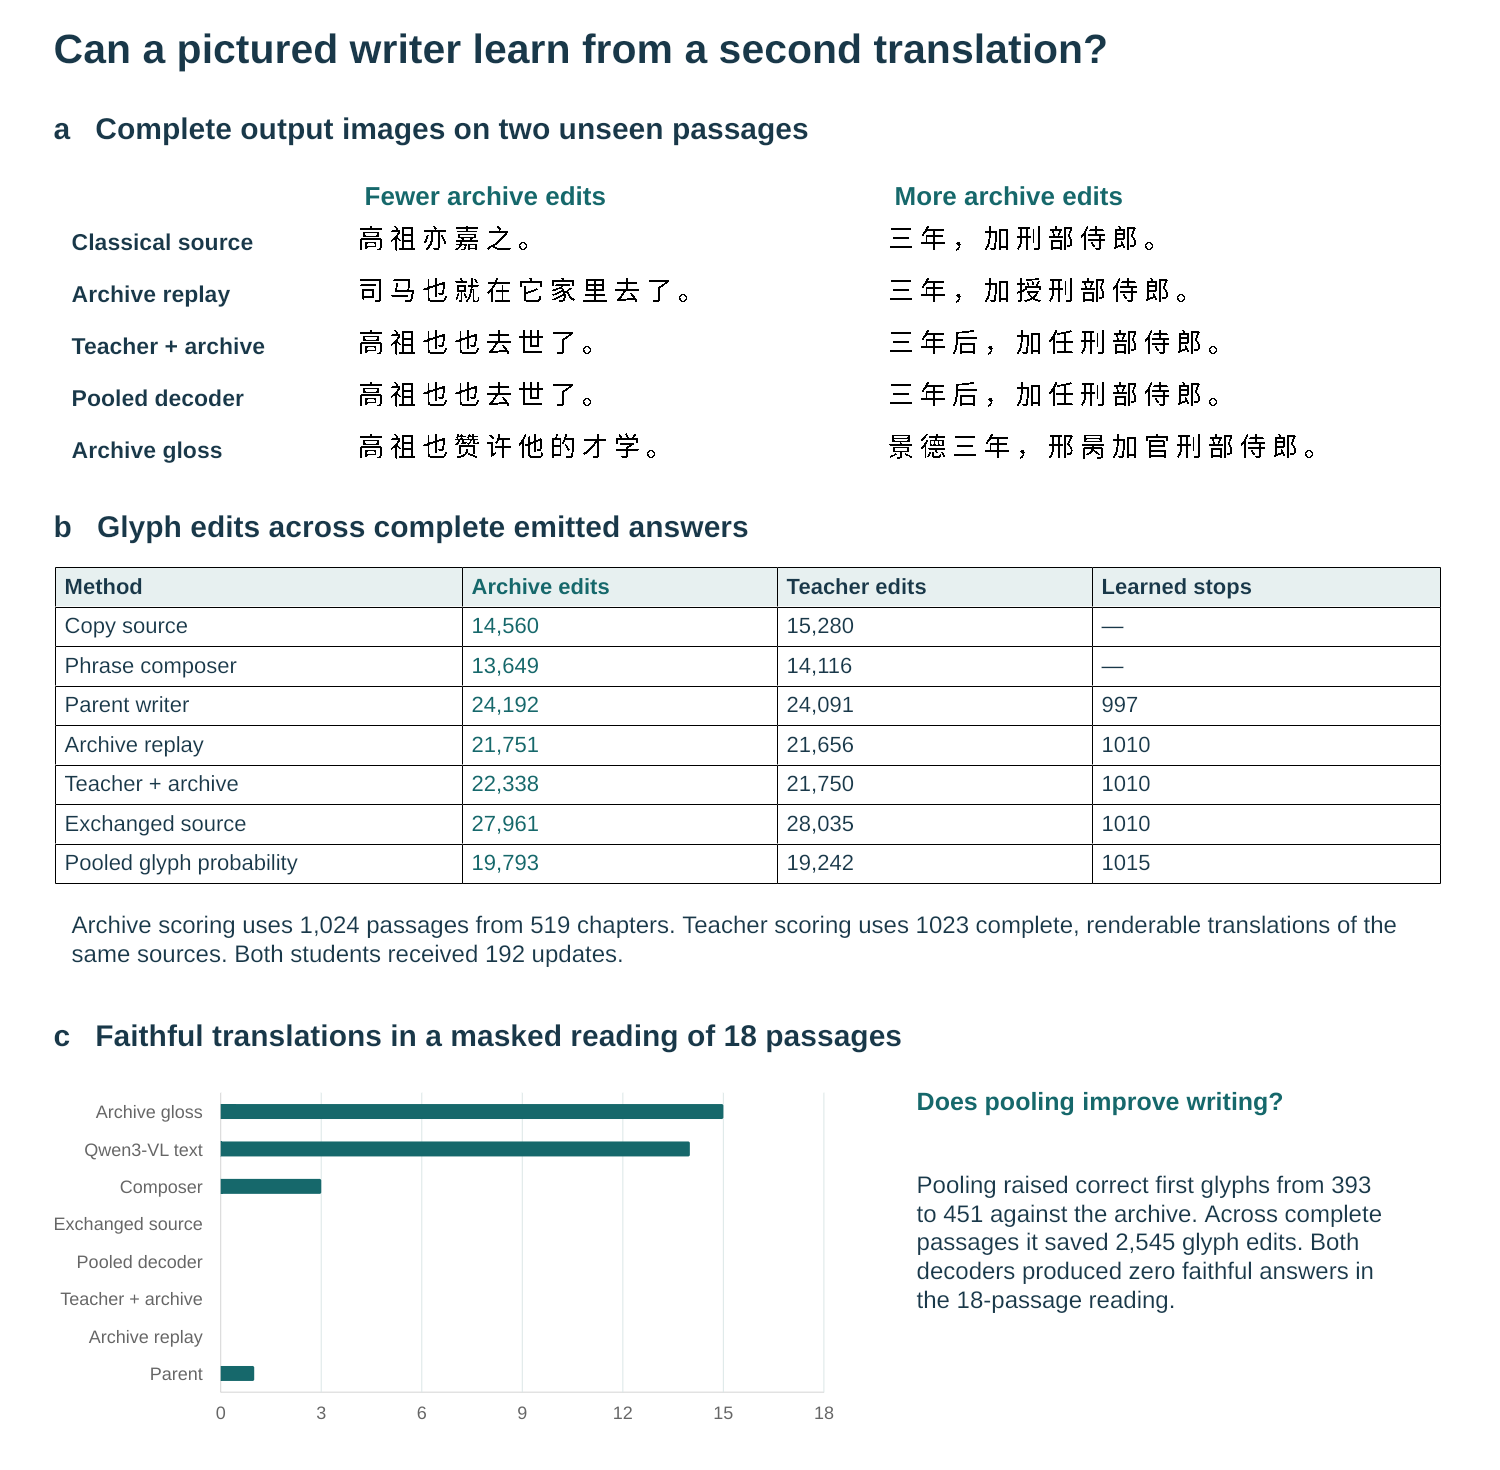
\includegraphics[width=.84\textwidth]{figures/Figure_61_paired_student.png}
\caption{\DIFaddFL{\textbf{Pooling probability across identical ink improves glyph agreement but leaves complete meaning unresolved.} \textbf{a}, Original complete image streams for the first compact gain and loss of the teacher-supplemented writer relative to archive replay. All four streams used for selection were at most fifteen glyphs long. The pooled decoder uses the identical supplemented checkpoint. \textbf{b}, Physical edit totals against 24,088 archive cells and 25,025 eligible teacher cells. Stops count complete generation before the 96-cell ceiling. Source exchange preserves the output multiset. \textbf{c}, Faithful answers in eighteen source-marker passages. The pretrained teacher read typed sources. The pooled writer was read in a second masked comparison of the same passages. Physical improvement and faithful modern translation have different denominators.}}
\label{fig:paired-student}
\end{figure*}
\begin{figure*}[p]
\centering
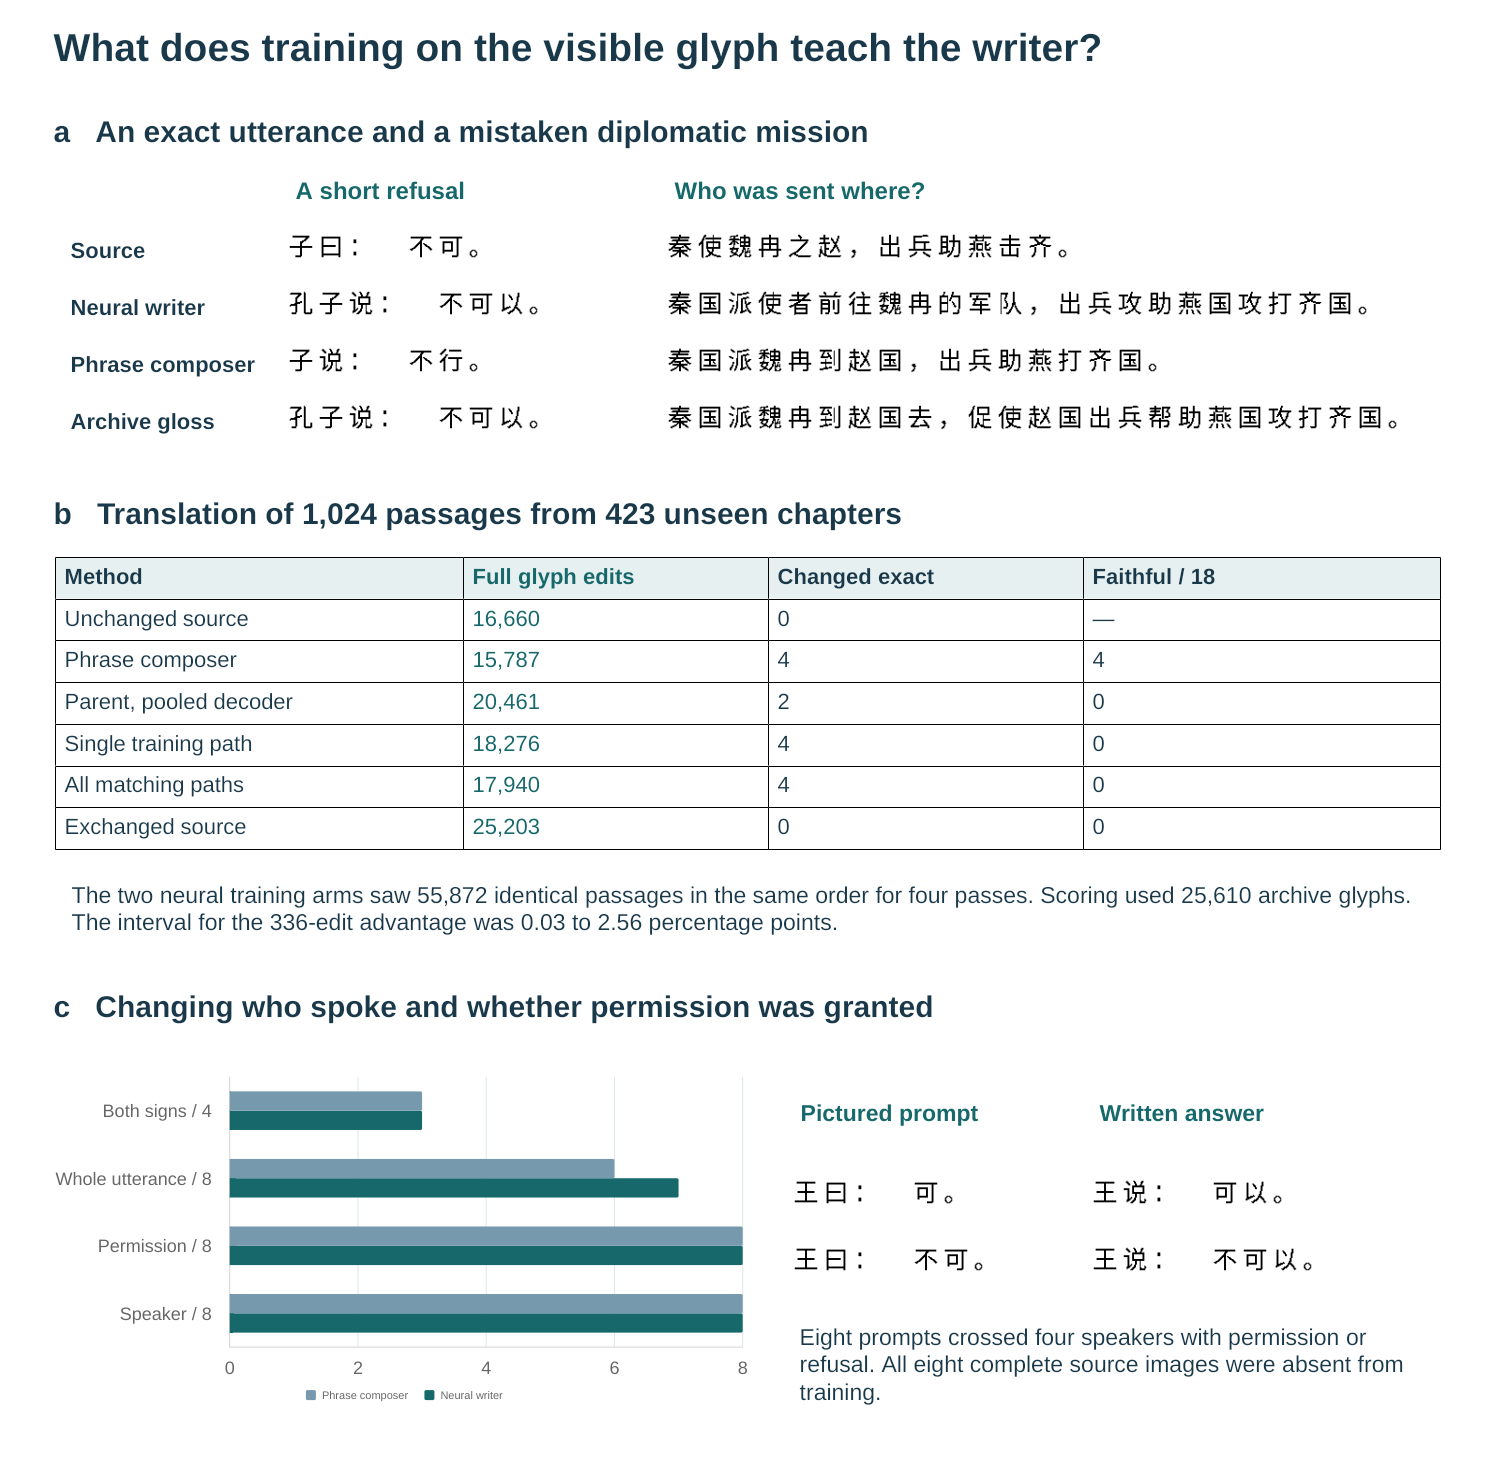
\includegraphics[width=.84\textwidth]{figures/Figure_62_visible_likelihood.png}
\caption{\DIFaddFL{\textbf{Credit for matching physical ink improves glyph accuracy and supports a limited grammatical contrast.} \textbf{a}, Complete original pictures for the first exact neural answer with two or more lexical edits to the source and for an envoy mission with an incorrect participant role. \textbf{b}, Whole-stream edit and masked faithfulness scores. Changed exact counts only passages where the recorded modern gloss differs from the input. \textbf{c}, Masked readings of eight source pictures crossing speaker and polarity. The final pair measure has four opportunities; the others have eight. The right-hand examples show actual model outputs when the king grants and denies permission. This construction was chosen after finding the initial exact refusal.}}
\label{fig:visible-likelihood}
\end{figure*}
\begin{figure*}[p]
\centering
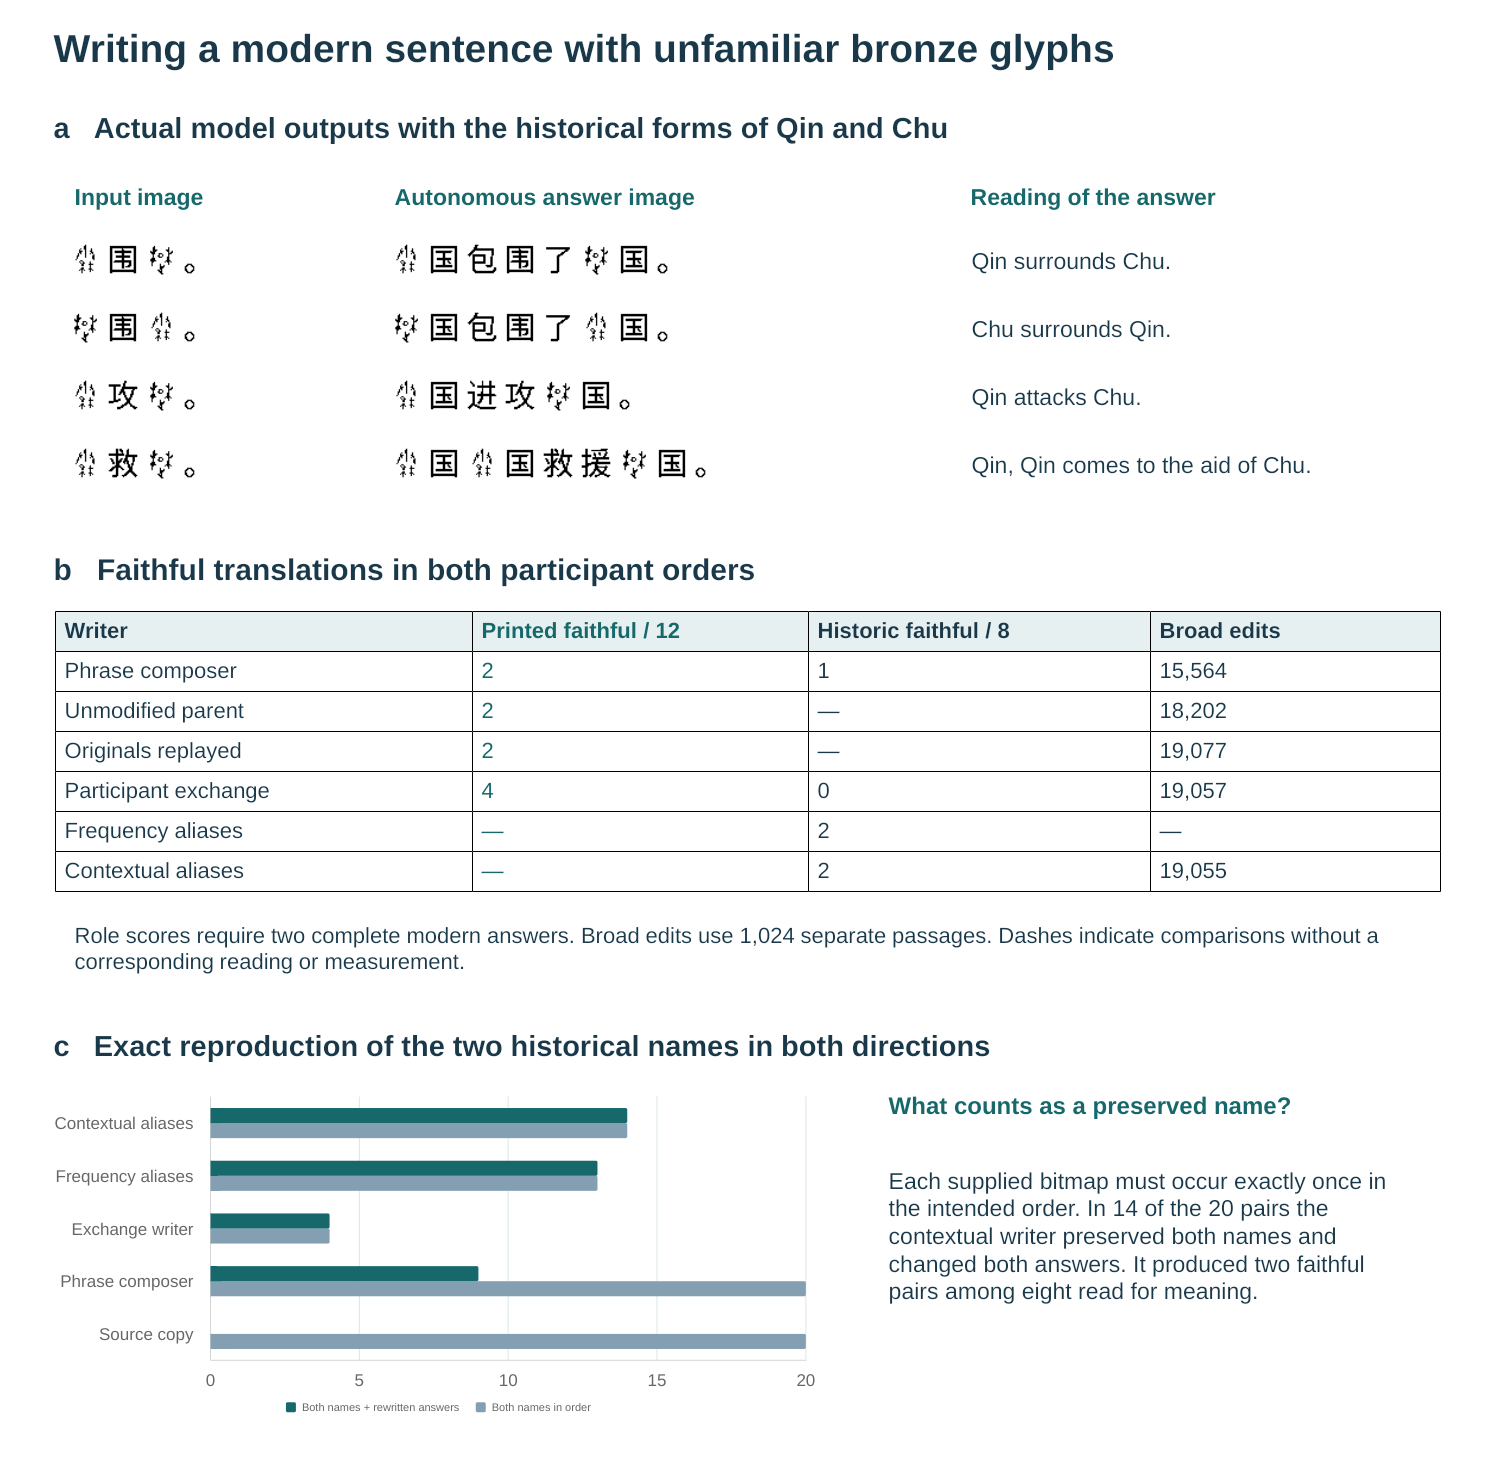
\includegraphics[width=.84\textwidth]{figures/Figure_63_event_roles.png}
\caption{\DIFaddFL{\textbf{Participant exchange and generation with historical Chinese names.} \textbf{a}, Four complete inputs and autonomous answers using the catalogue bronze forms of Qin (B11149) and Chu (B08953). The first two rows reverse who surrounds whom. The last repeats the rescuer. English readings accompany the emitted pixels. \textbf{b}, Faithful modern wording in both directions of a pair. The two reading samples and the broad passage edit counts measure different outcomes. \textbf{c}, Number of pairs among twenty in which both supplied name images occur exactly once in the intended order in both answers. The second bar also requires both outputs to differ from their inputs. Copying preserves every name and modernizes no passage.}}
\label{fig:event-roles}
\end{figure*}
\begin{figure*}[p]
\centering
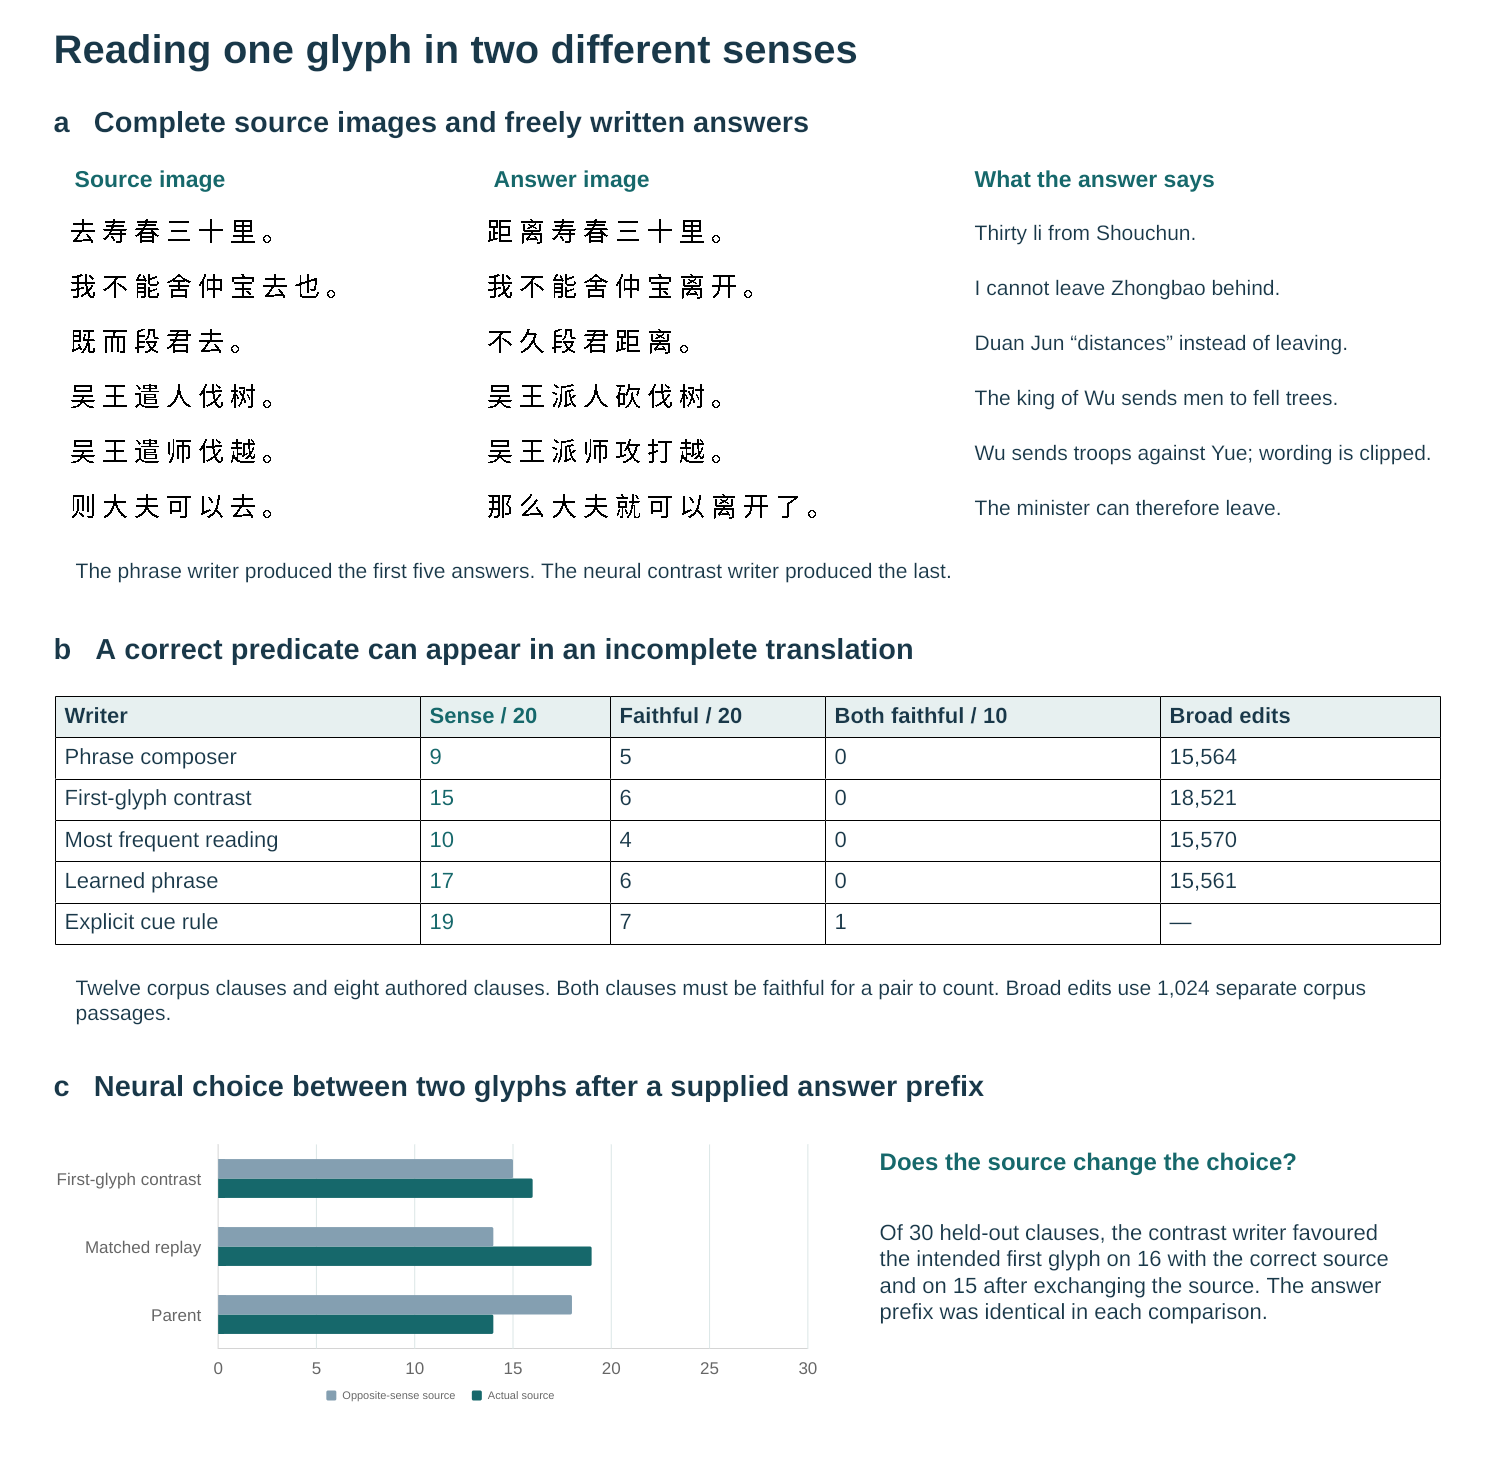
\includegraphics[width=.84\textwidth]{figures/Figure_64_predicate_context.png}
\caption{\DIFaddFL{\textbf{Contextual readings of the same physical Chinese verb.} \textbf{a}, Complete, unmodified image streams. The first two examples distinguish distance from departure. The third chooses distance when a person leaves. The fourth and fifth use the same subject with different meanings of the second verb. The last answer is a successful neural modernization in the original test. \textbf{b}, Free responses to twelve chapter-held-out clauses and eight authored contrasts. The explicit cue rule receives the tested predicate. Broad edits compare 1,024 separate outputs with their corpus glosses. The cue control applies only to the targeted contrasts. \textbf{c}, Number of clauses in the original test for which the model assigns more copy-plus-exemplar probability to the intended first glyph than to a specified rival. The decoder receives the same recorded answer prefix when the source changes.}}
\label{fig:predicate-context}
\end{figure*}
\begin{figure*}[p]
\centering
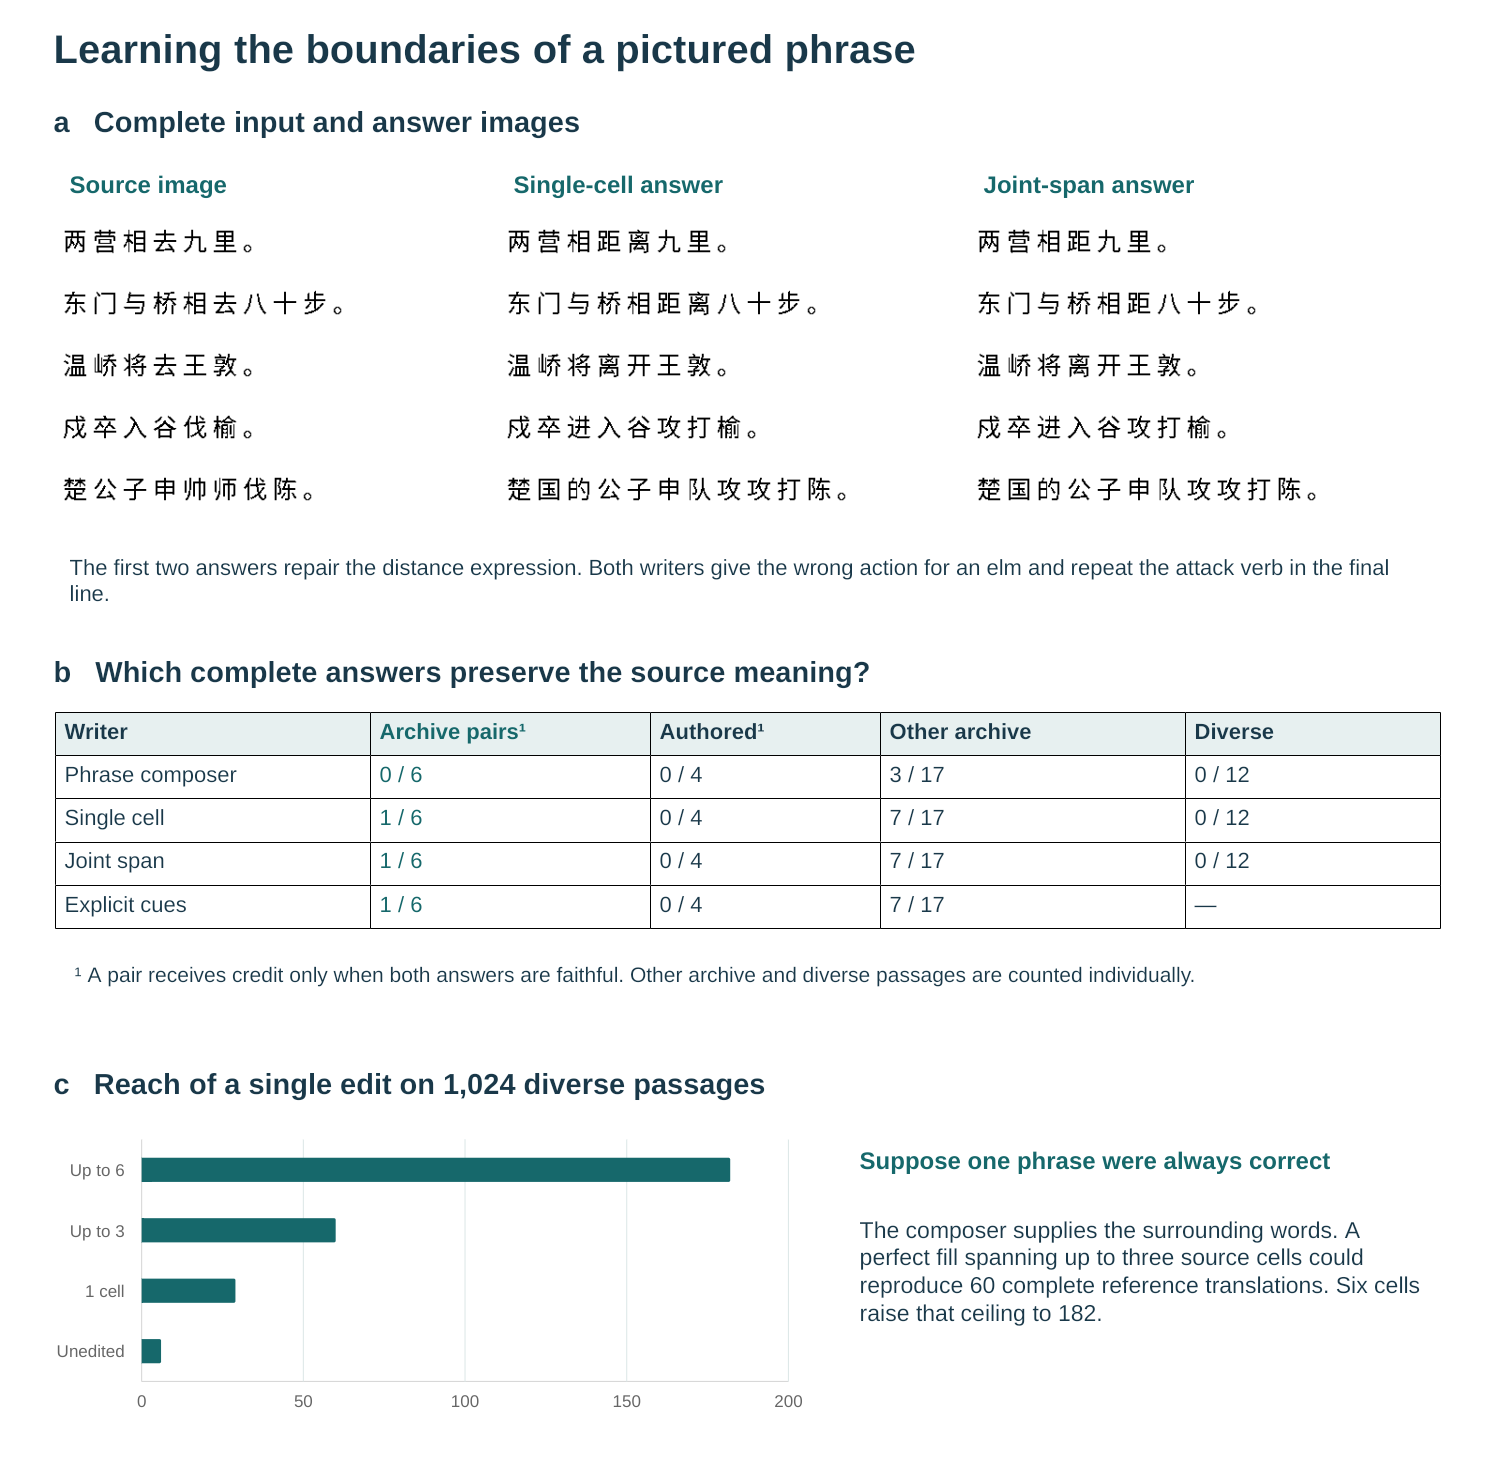
\includegraphics[width=.84\textwidth]{figures/Figure_65_phrase_boundary.png}
\caption{\DIFaddFL{\textbf{Learning where a pictured translation begins and ends.} \textbf{a}, Complete input and output images from two writers sharing the same verb-sense predictions. The first two sources are authored contrasts. The third comes from a fresh archive chapter. The fourth is an authored felling clause and the fifth is archival. Both writers incorrectly attack an elm and duplicate the attack verb in the last example. \textbf{b}, Faithfulness of independently written modern Chinese. The first two columns require both complete answers in each pair. The other two columns count individual clauses. \textbf{c}, Exact reference images attainable on 1,024 passages if one source span could emit any correct target strip. Outside that span the original composer supplies all pixels. This calculation uses the reference at evaluation.}}
\label{fig:phrase-boundary}
\end{figure*}
\begin{figure*}[p]
\centering
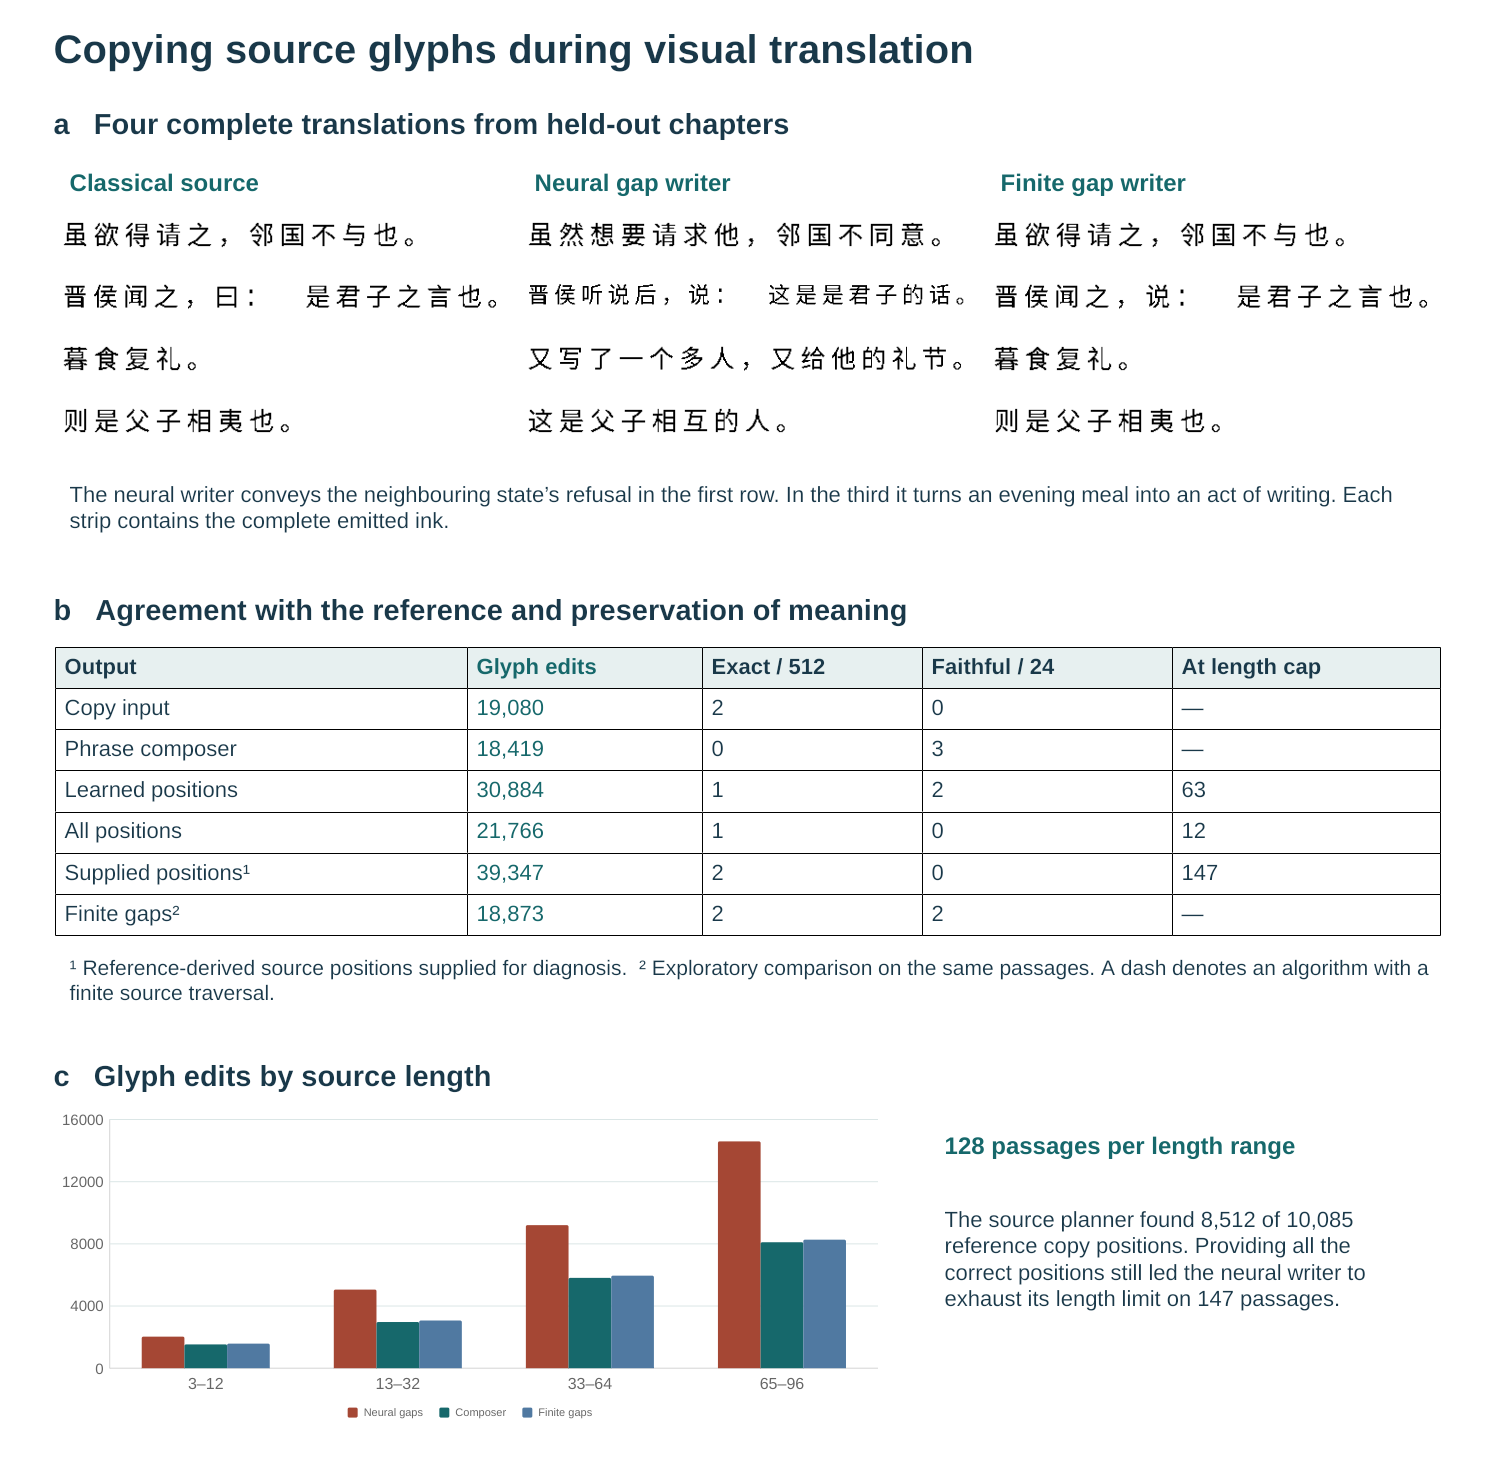
\includegraphics[width=.84\textwidth]{figures/Figure_66_anchor_gap.png}
\caption{\DIFaddFL{\textbf{Translating the intervals between copied source images.}
\textbf{a}, Four complete source and output strips from the fixed reading roster. The first two illustrate the neural writer's two credited answers, including a repeated copula in the second. The remaining examples concern observance of ritual at supper and injury to a family relationship. Both writers miss the meaning. \textbf{b}, Physical edits on 512 unseen passages and complete-meaning judgments on 24. Supplying reference-derived source positions leaves their target offsets unknown. An exploratory finite writer uses the same learned planner. The length cap is 192 emitted cells. \textbf{c}, Total edits in four equally populated source-length ranges. Each count compares the complete generated sequence with one published translation. Alternative faithful wording may incur edits.}}
\label{fig:anchor-gap}
\end{figure*}
\begin{figure*}[p]
\centering
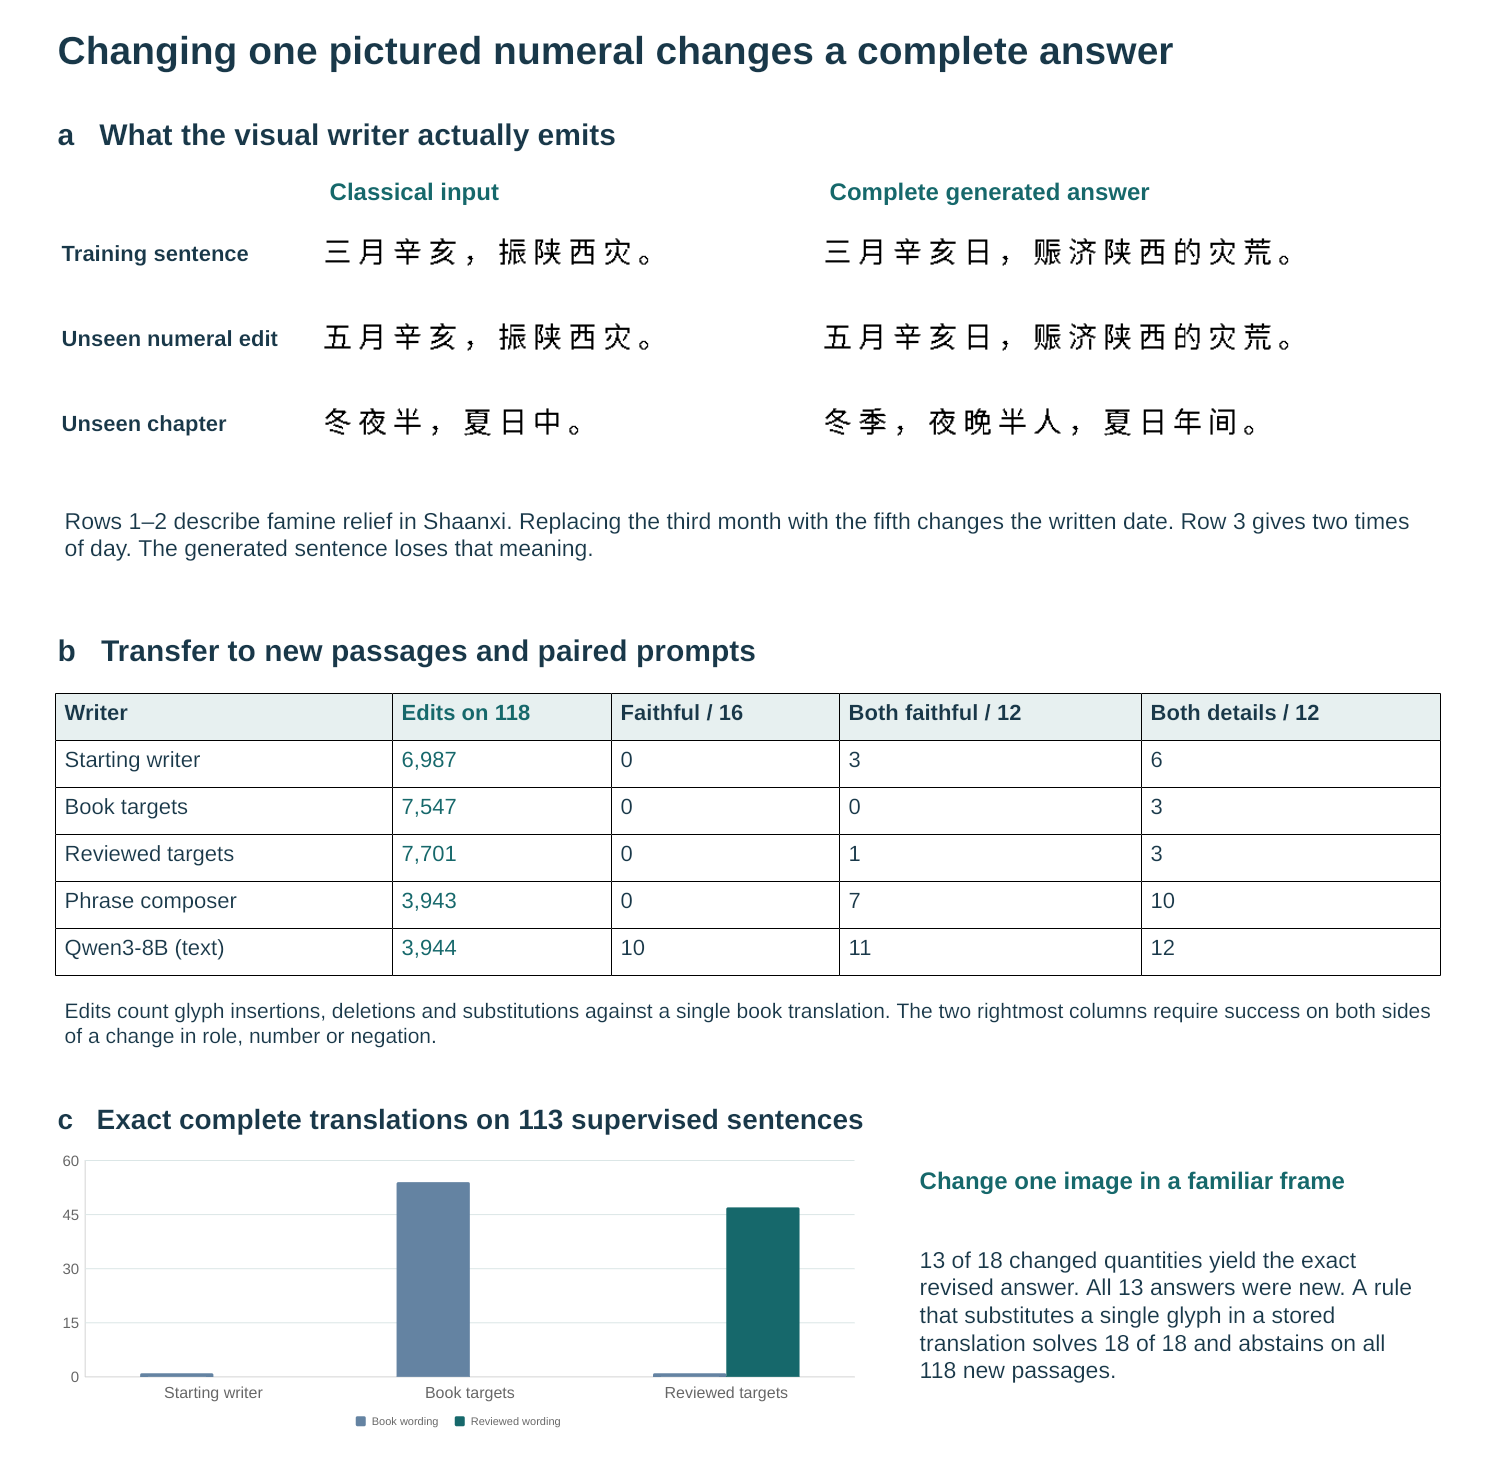
\includegraphics[width=.84\textwidth]{figures/Figure_67_screened_targets.png}
\caption{\DIFaddFL{\textbf{Transfer of learned translations after a change in a pictured quantity.}
\textbf{a}, Complete input and freely generated output strips, displayed from saved ink. The first row is a supervised sentence. In the second, a substitution changes the date of famine relief from the third month to the fifth. The third is a failed translation from a reserved chapter. \textbf{b}, Total edits on 118 passages, complete meanings on a fixed reading of 16, and pairs conveying both meanings or both tested details among twelve minimal pairs. Qwen3-8B received text and ran separately after training. \textbf{c}, Exact matches against two target wordings for 113 supervised sentences. The numeral and displacement probes change one input cell while keeping the surrounding sentence. An image analogy using the 113 stored examples also answers all 18 numeral edits and abstains on the new passages.}}
\label{fig:screened-targets}
\end{figure*}
\begin{figure*}[p]
\centering
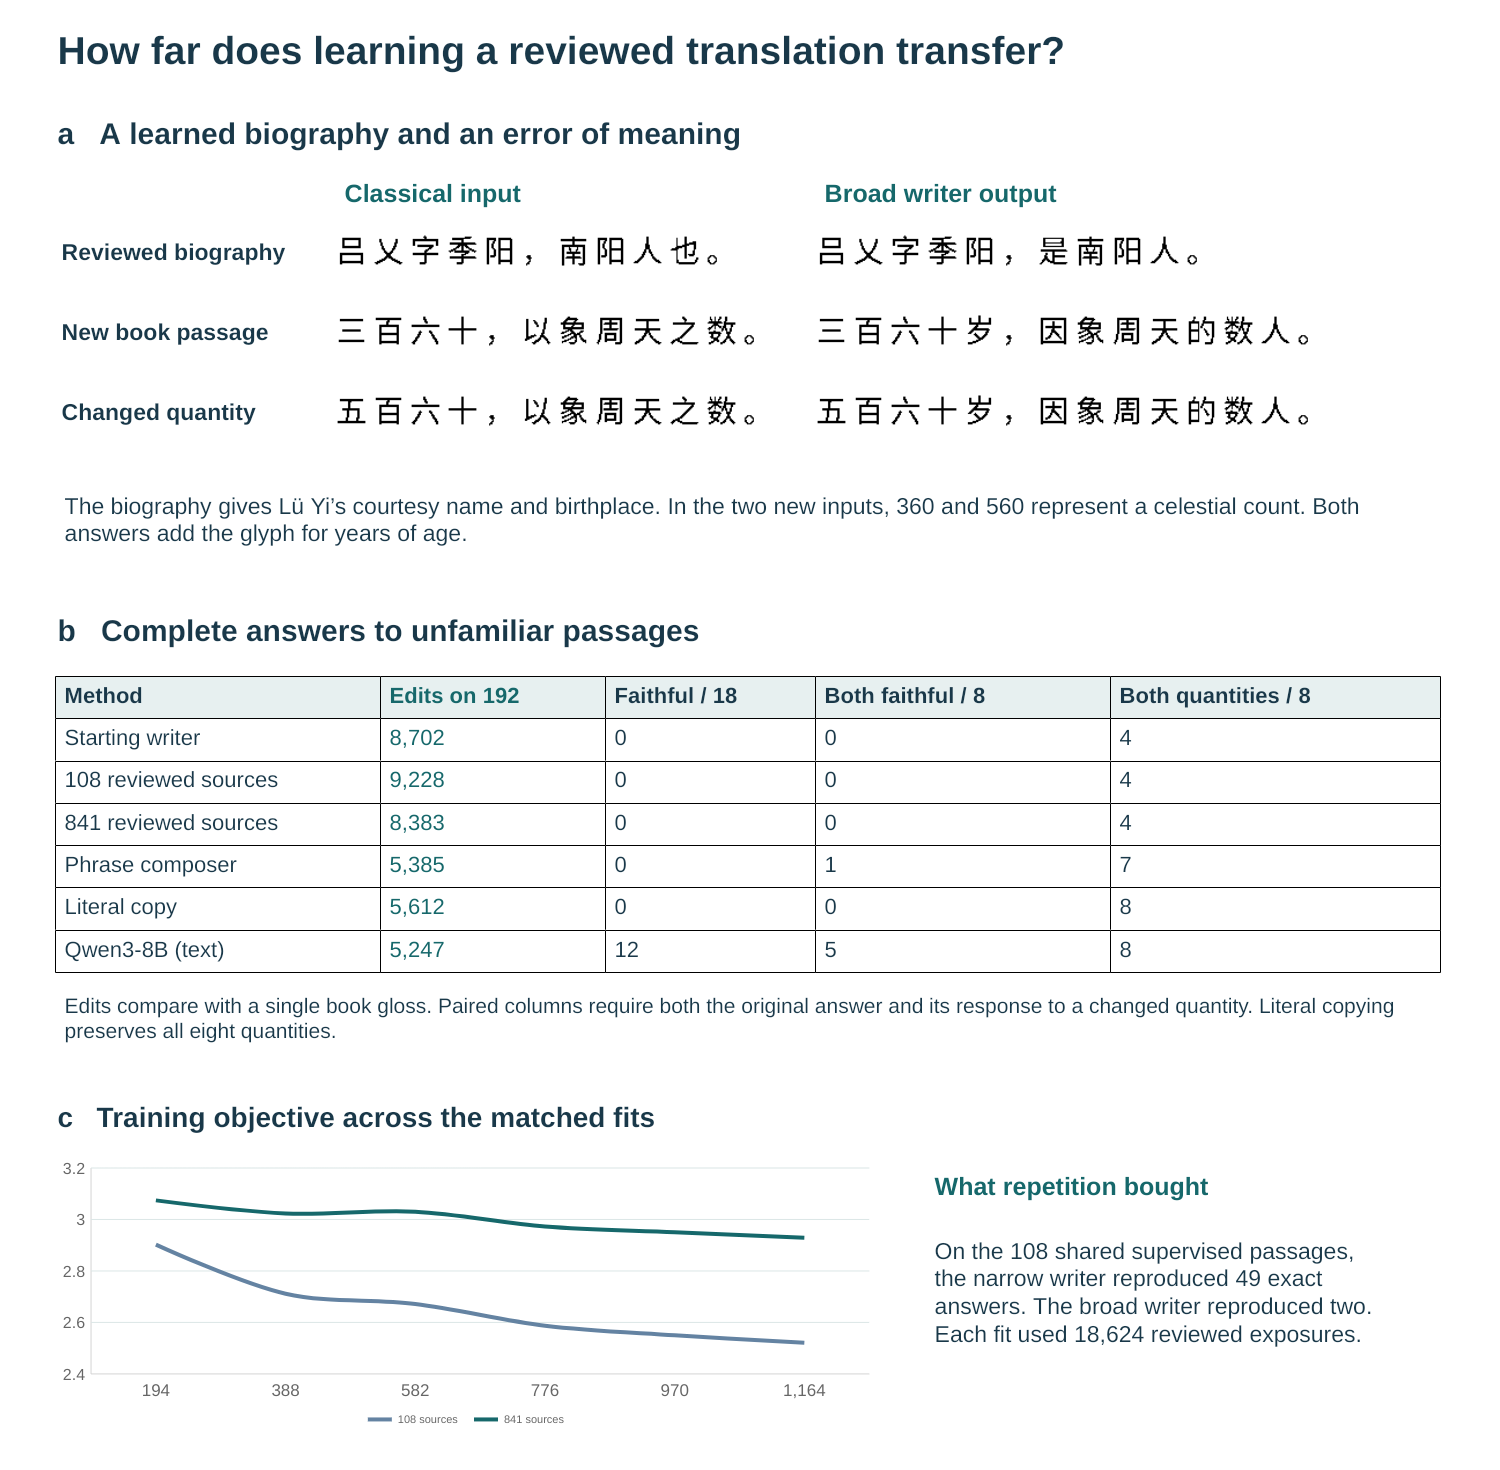
\includegraphics[width=.84\textwidth]{figures/Figure_68_translation_coverage.png}
\caption{\DIFaddFL{\textbf{Transfer from reviewed translations to new chapters.} \textbf{a}, Complete source and emitted images from the 841-source writer. In the supervised biography the model adds the modern copula and removes a classical sentence-final particle. The two celestial counts elicit the same erroneous unit of age. \textbf{b}, One model reader graded method-masked translations of eighteen passages and eight pairs. Quantity credit requires the correct referent as well as the number. The reference gloss received nine of eighteen whole credits under the source-only rubric. \textbf{c}, Training loss averaged over successive blocks of 194 updates. Each writer received the same book replay, number of supplemental exposures and per-batch padding. The broader writer saw each reviewed translation fewer times.}}
\label{fig:translation-coverage}
\end{figure*}
\begin{figure*}[p]
\centering
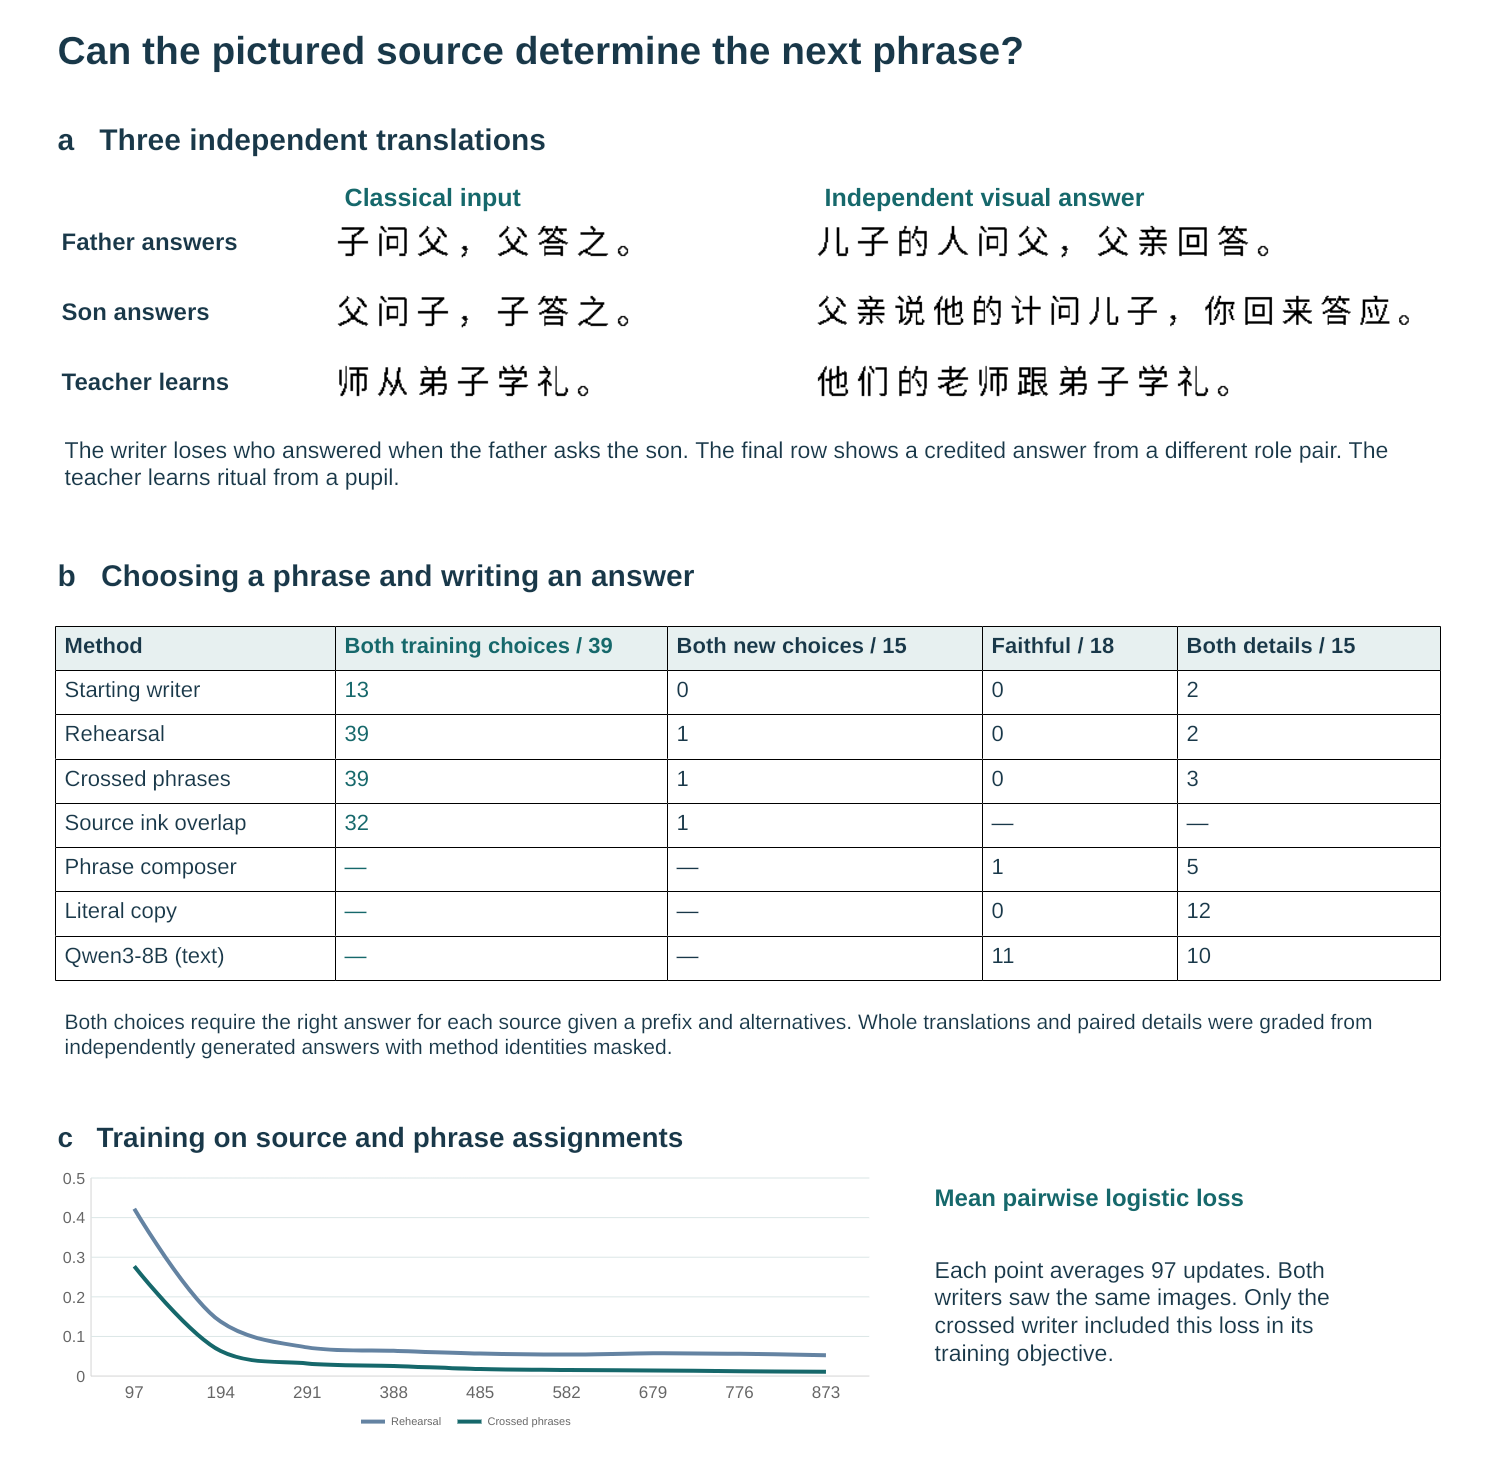
\includegraphics[width=.84\textwidth]{figures/Figure_69_context_phrases.png}
\caption{\DIFaddFL{\textbf{Choosing between competing pictured phrases and generating a translation.} \textbf{a}, Complete emitted strips for the first role reversal in the fixed roster and a separately selected credited reading. In the first source the father answers the son. The second exchanges their roles. The third source describes a teacher learning from a pupil. \textbf{b}, Conditional scores use a supplied common prefix and both alternative phrases. Autonomous writers receive only the source. Both-detail credit requires an answer expressing the designated detail on each side. The text teacher receives the source transcription. \textbf{c}, Mean pairwise logistic loss on training examples, averaged over successive groups of 97 updates. Each arm saw 3,492 pair presentations. Rehearsal records this value for comparison.}}
\label{fig:context-phrases}
\end{figure*}
\begin{figure*}[p]
\centering
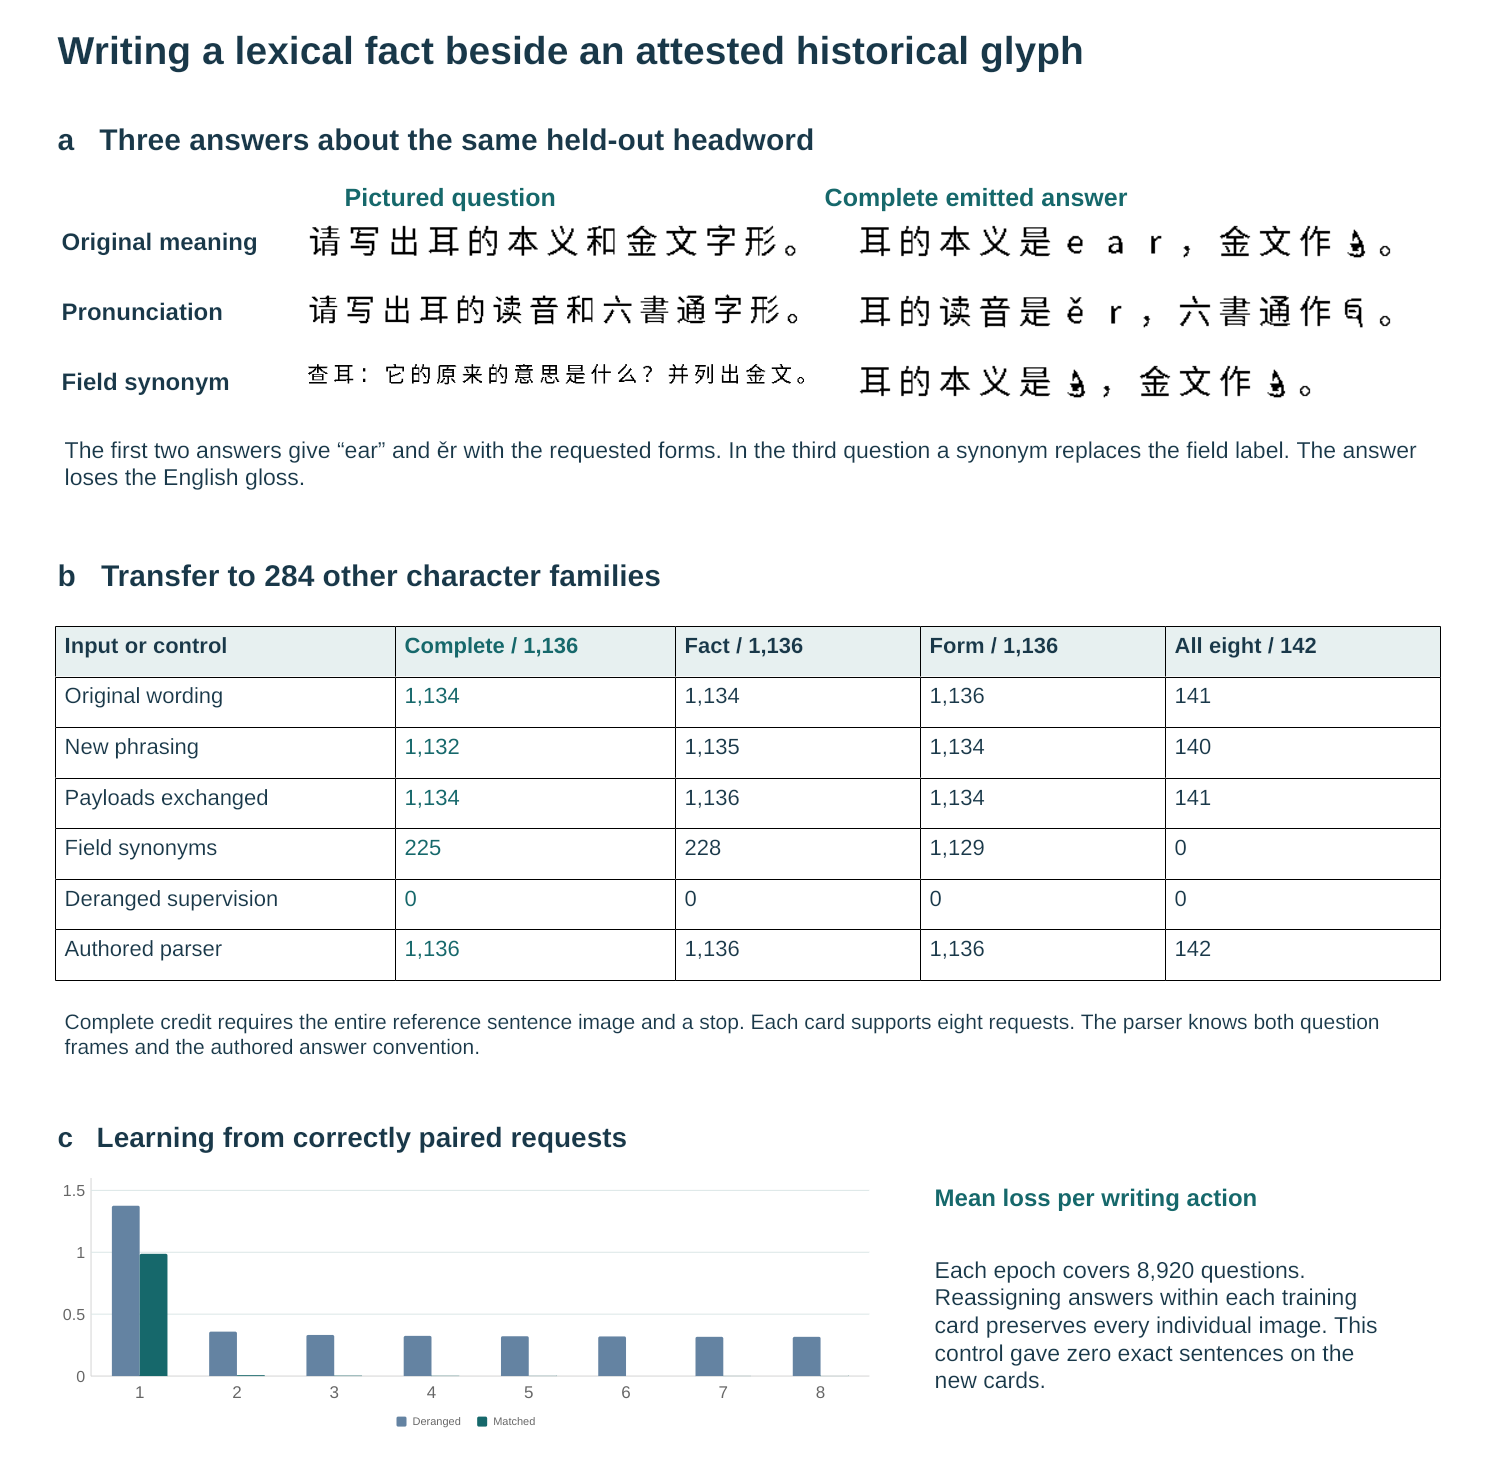
\includegraphics[width=.84\textwidth]{figures/Figure_70_pictured_entries.png}
\caption{\DIFaddFL{\textbf{A recurrent writer combines a lexical fact and historical ink.} \textbf{a}, Pictured questions and complete model answers for the first held-out entry. The third row shows the first answer lost when an alternative term replaced the field label. Hanziyuan supplies the source gloss and historical exemplars. \textbf{b}, Each of 142 two-entry cards supports eight independently scored requests. The relocation intervention swaps values for corresponding labels between the two records. The alternate question frame retains the visible field names. The synonym condition changes them. \textbf{c}, Mean training loss per physical span or stop over eight epochs. The control reassigns the eight targets within each training card.}}
\label{fig:pictured-entries}
\end{figure*}
\begin{figure*}[p]
\centering
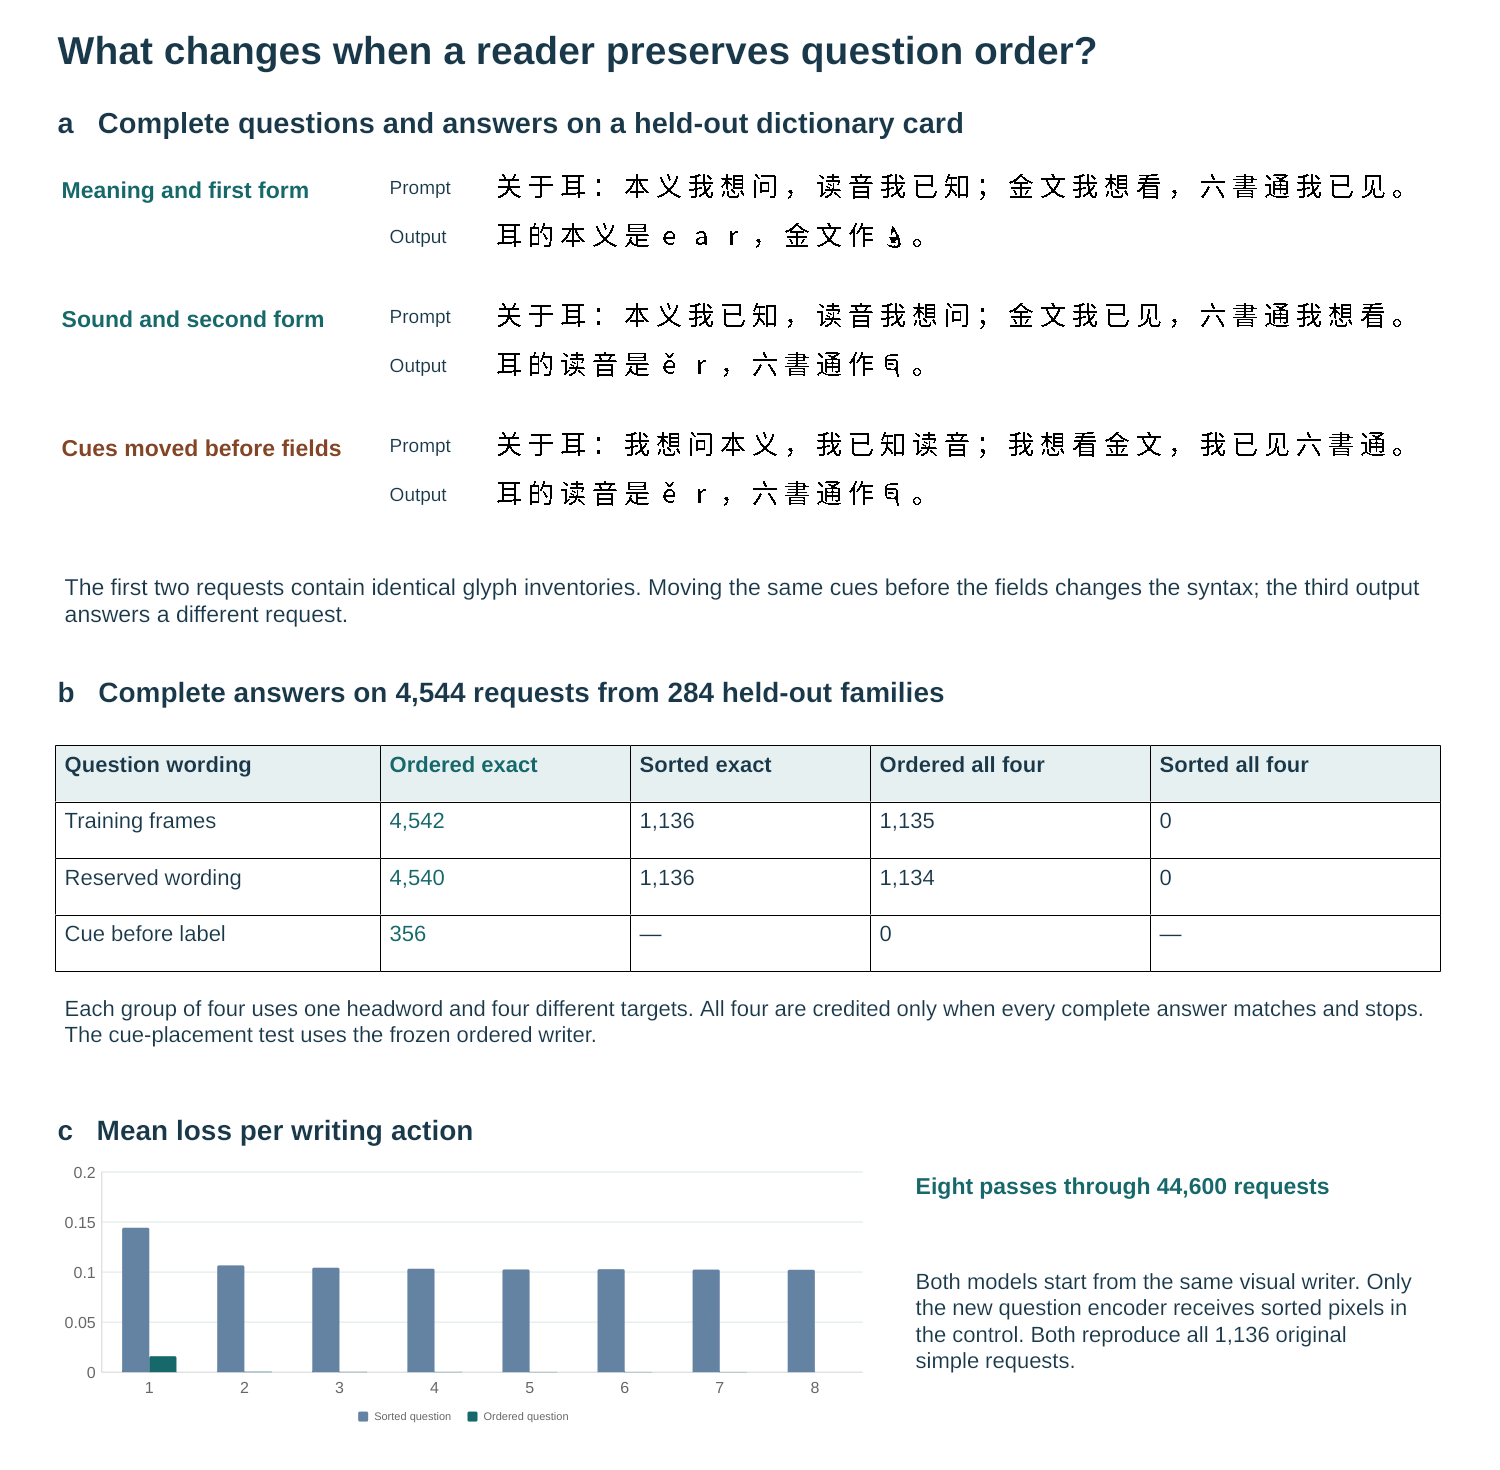
\includegraphics[width=.84\textwidth]{figures/Figure_71_question_order.png}
\caption{\DIFaddFL{\textbf{Reading order controls which facts the writer emits.} \textbf{a}, Two requests from the first held-out group and their emitted sentences. The same images of the headword, fields and historical stages appear in both questions. The third row shows the first exact response lost when the status expressions moved before their fields. All six strips are original question or response pixels. \textbf{b}, Each of 1,136 groups has four distinct target images. The sorted control receives a canonical ordering of glyphs through the additional encoder. The source reader and its original visual field matches are identical across arms. The dash denotes an unmeasured control. \textbf{c}, Both models learned on the same 35,680 role-sensitive requests and 8,920 simple requests per epoch.}}
\label{fig:question-order}
\end{figure*}
\begin{figure*}[p]
\centering
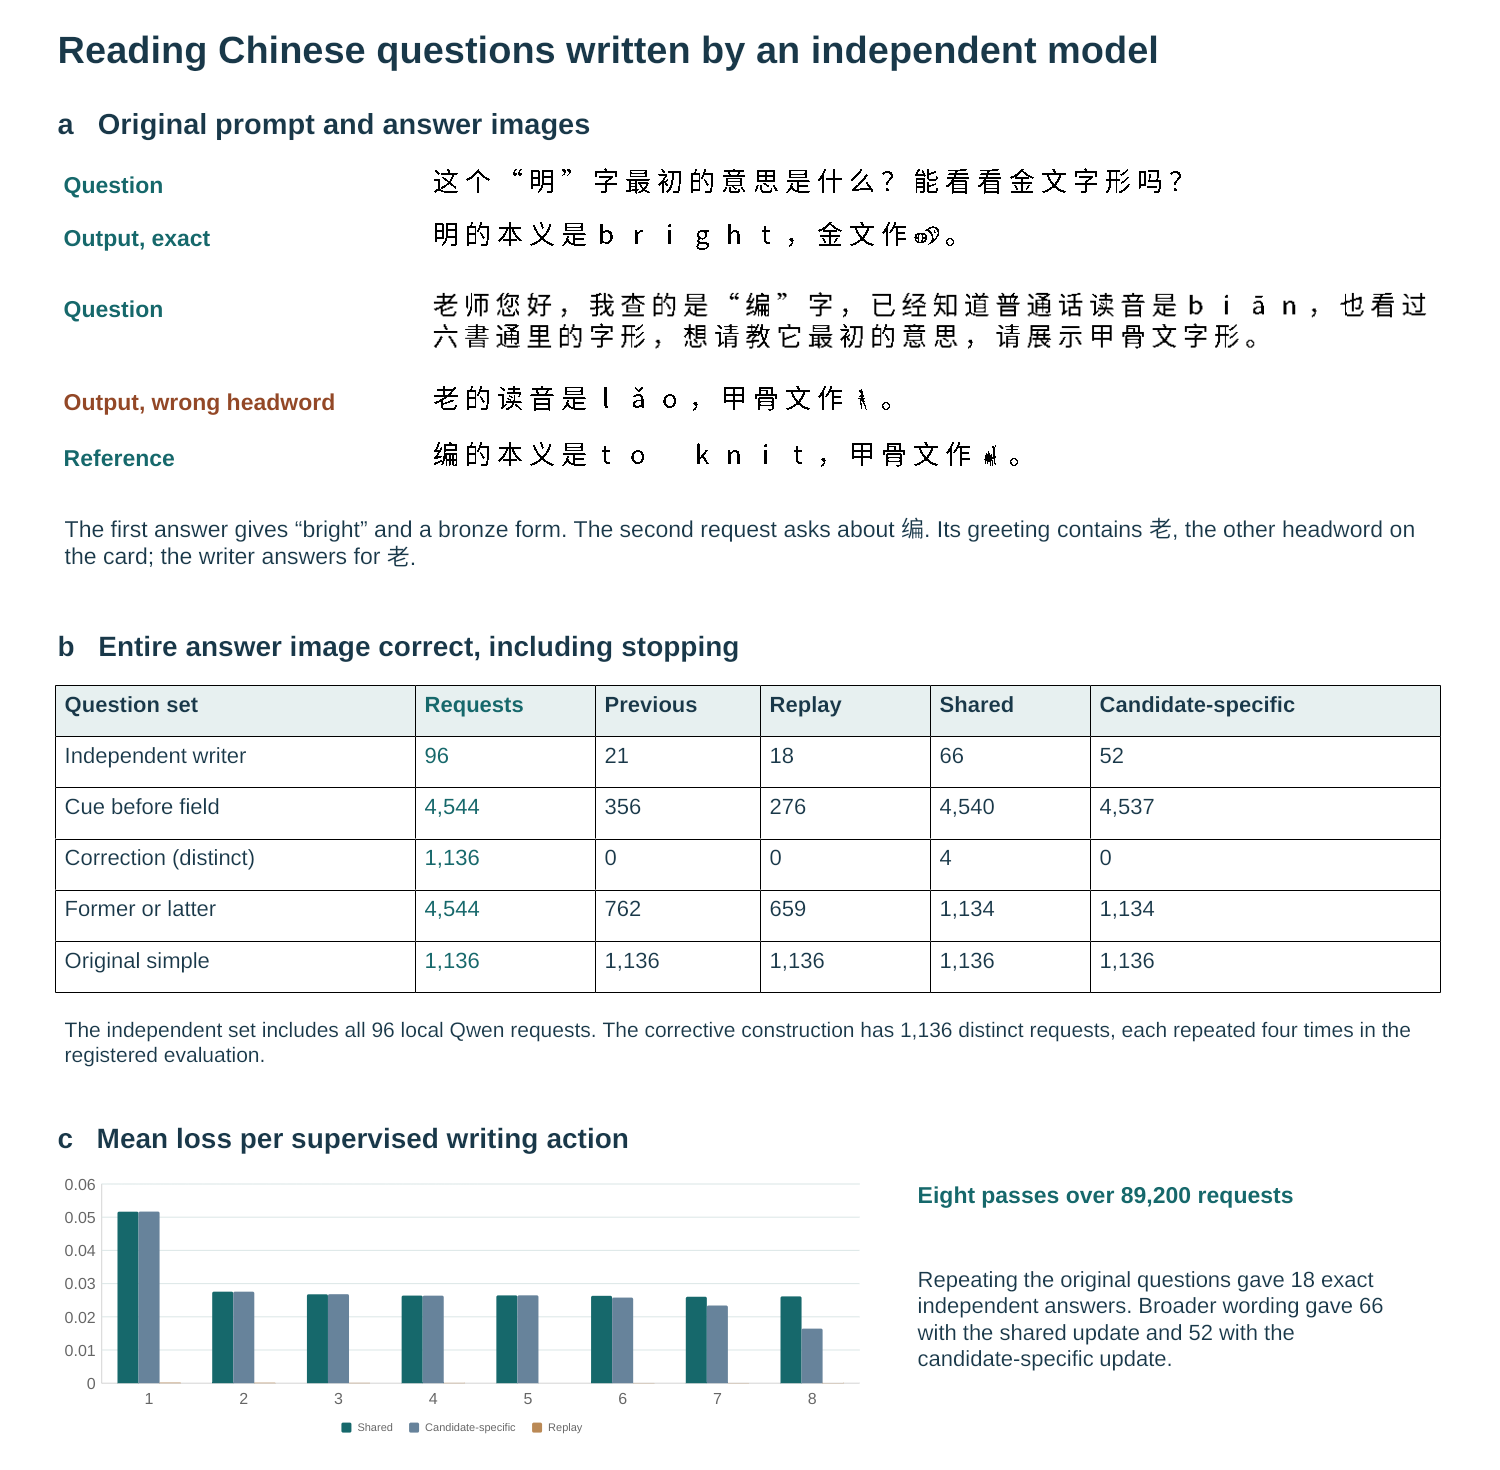
\includegraphics[width=.84\textwidth]{figures/Figure_72_independent_questions.png}
\caption{\DIFaddFL{\textbf{Wording diversity improves answer selection on independently authored prompts.} \textbf{a}, The first clear gain and the first clear error of the shared-update writer on questions from local Qwen3-8B. The images show the generated answers, including the misplaced pronunciation and oracle form of the neighbouring entry. \textbf{b}, Strict complete-image and stop counts. In the corrections row, the 4,544 scheduled requests reduce to 1,136 distinct question--card--target combinations. \textbf{c}, Mean training loss over nonpadding actions for the three 51,777-parameter fits. The supplementary replay control repeats the original questions at the same target positions for the same number of updates.}}
\label{fig:independent-questions}
\end{figure*}
\begin{figure*}[p]
\centering
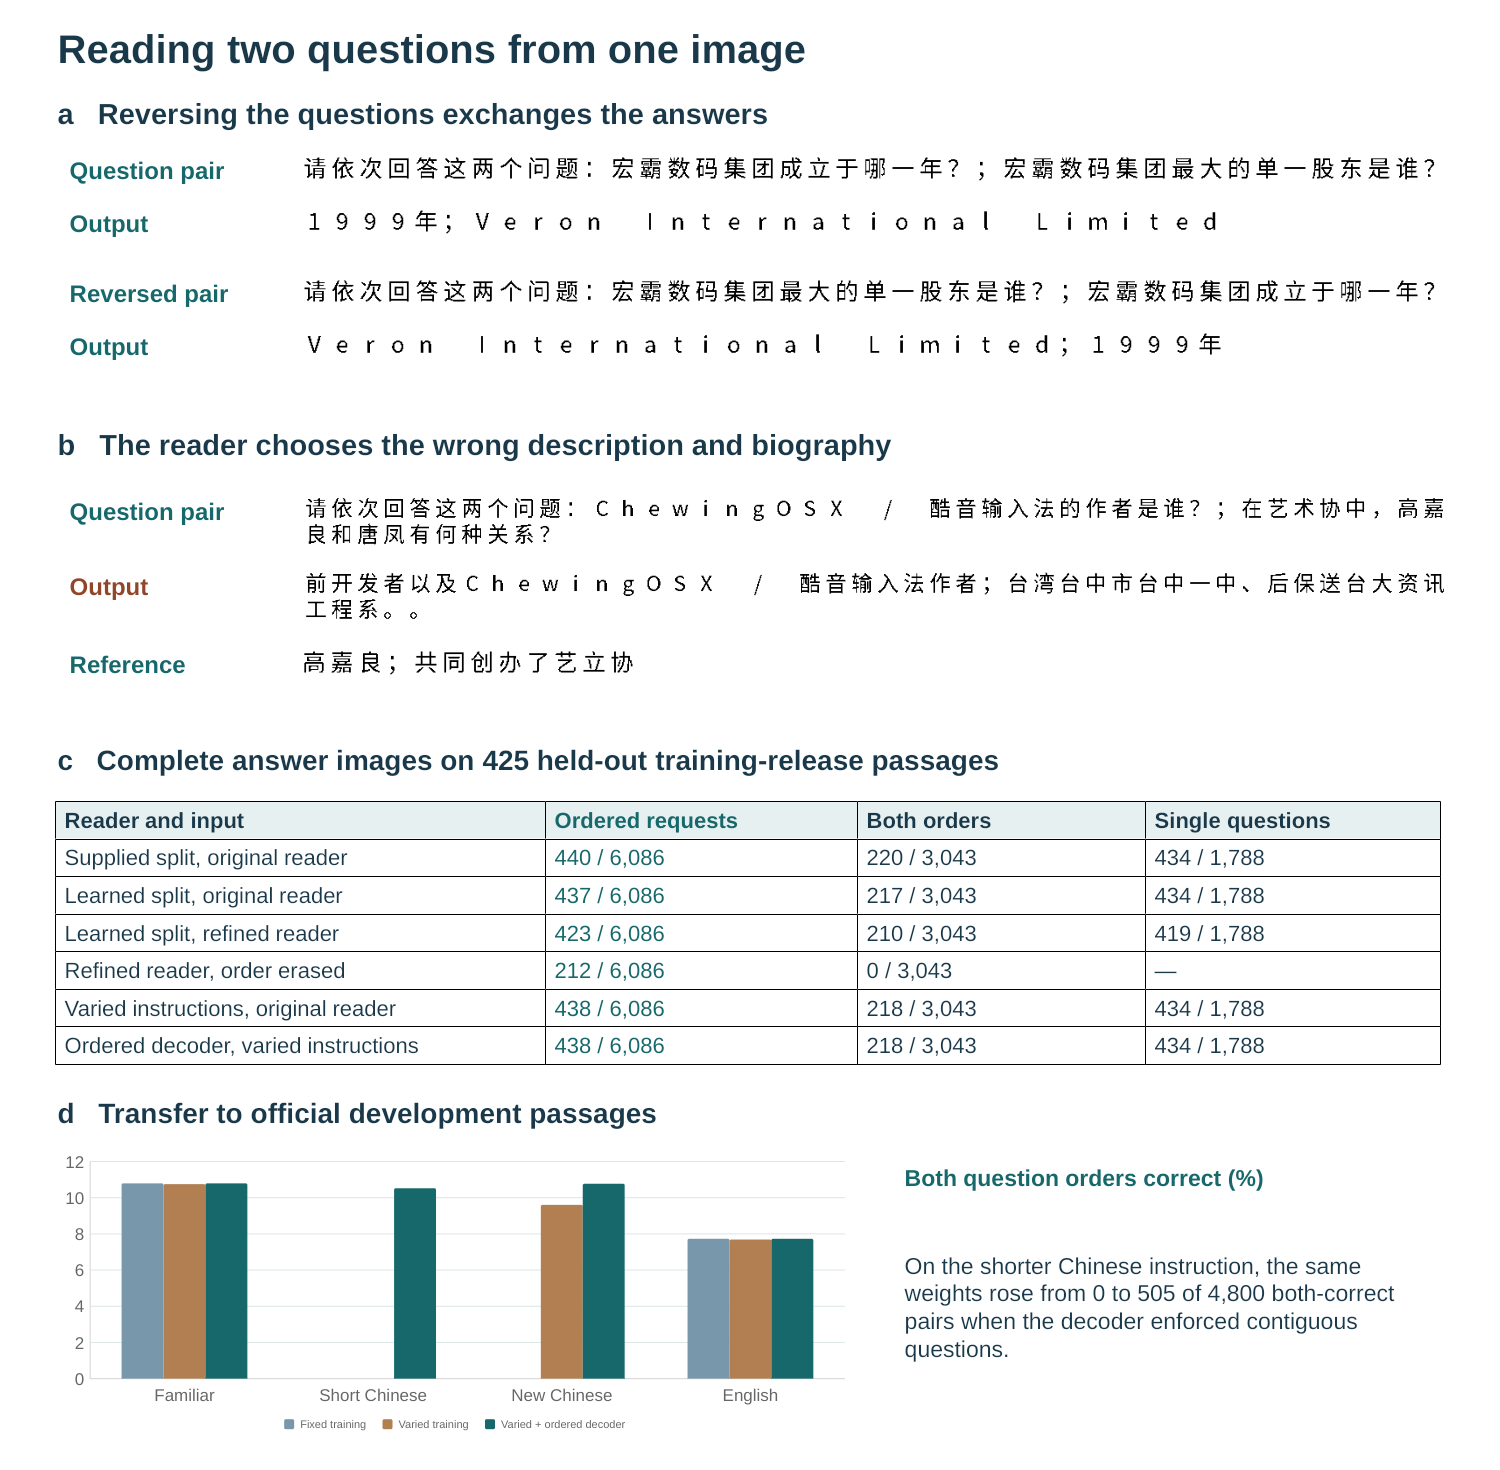
\includegraphics[width=.84\textwidth]{figures/Figure_73_paired_passage.png}
\caption{\DIFaddFL{\textbf{Question order transfers more reliably than question wording.} \textbf{a}, First exchanged pair for which the refined reader wrote both complete answers correctly. The same founding year and company name appear in reverse order. \textbf{b}, First failed request in corpus order, with the actual generated image and the reference. \textbf{c}, Internal held-out results. Each ordered request must match the entire target image and stop. Each distinct pair contributes two requests. The erased-order control receives the same question order for both requests. \textbf{d}, Percentage of official development pairs answered in both orders. All three conditions use the same frozen passage reader. The final two share planner weights. Constraining the reading regions recovered 505 of 4,800 pairs with the shorter Chinese instruction. All plotted values derive from saved answer pixels.}}
\label{fig:paired-passage}
\end{figure*}
\begin{figure*}[p]
\centering
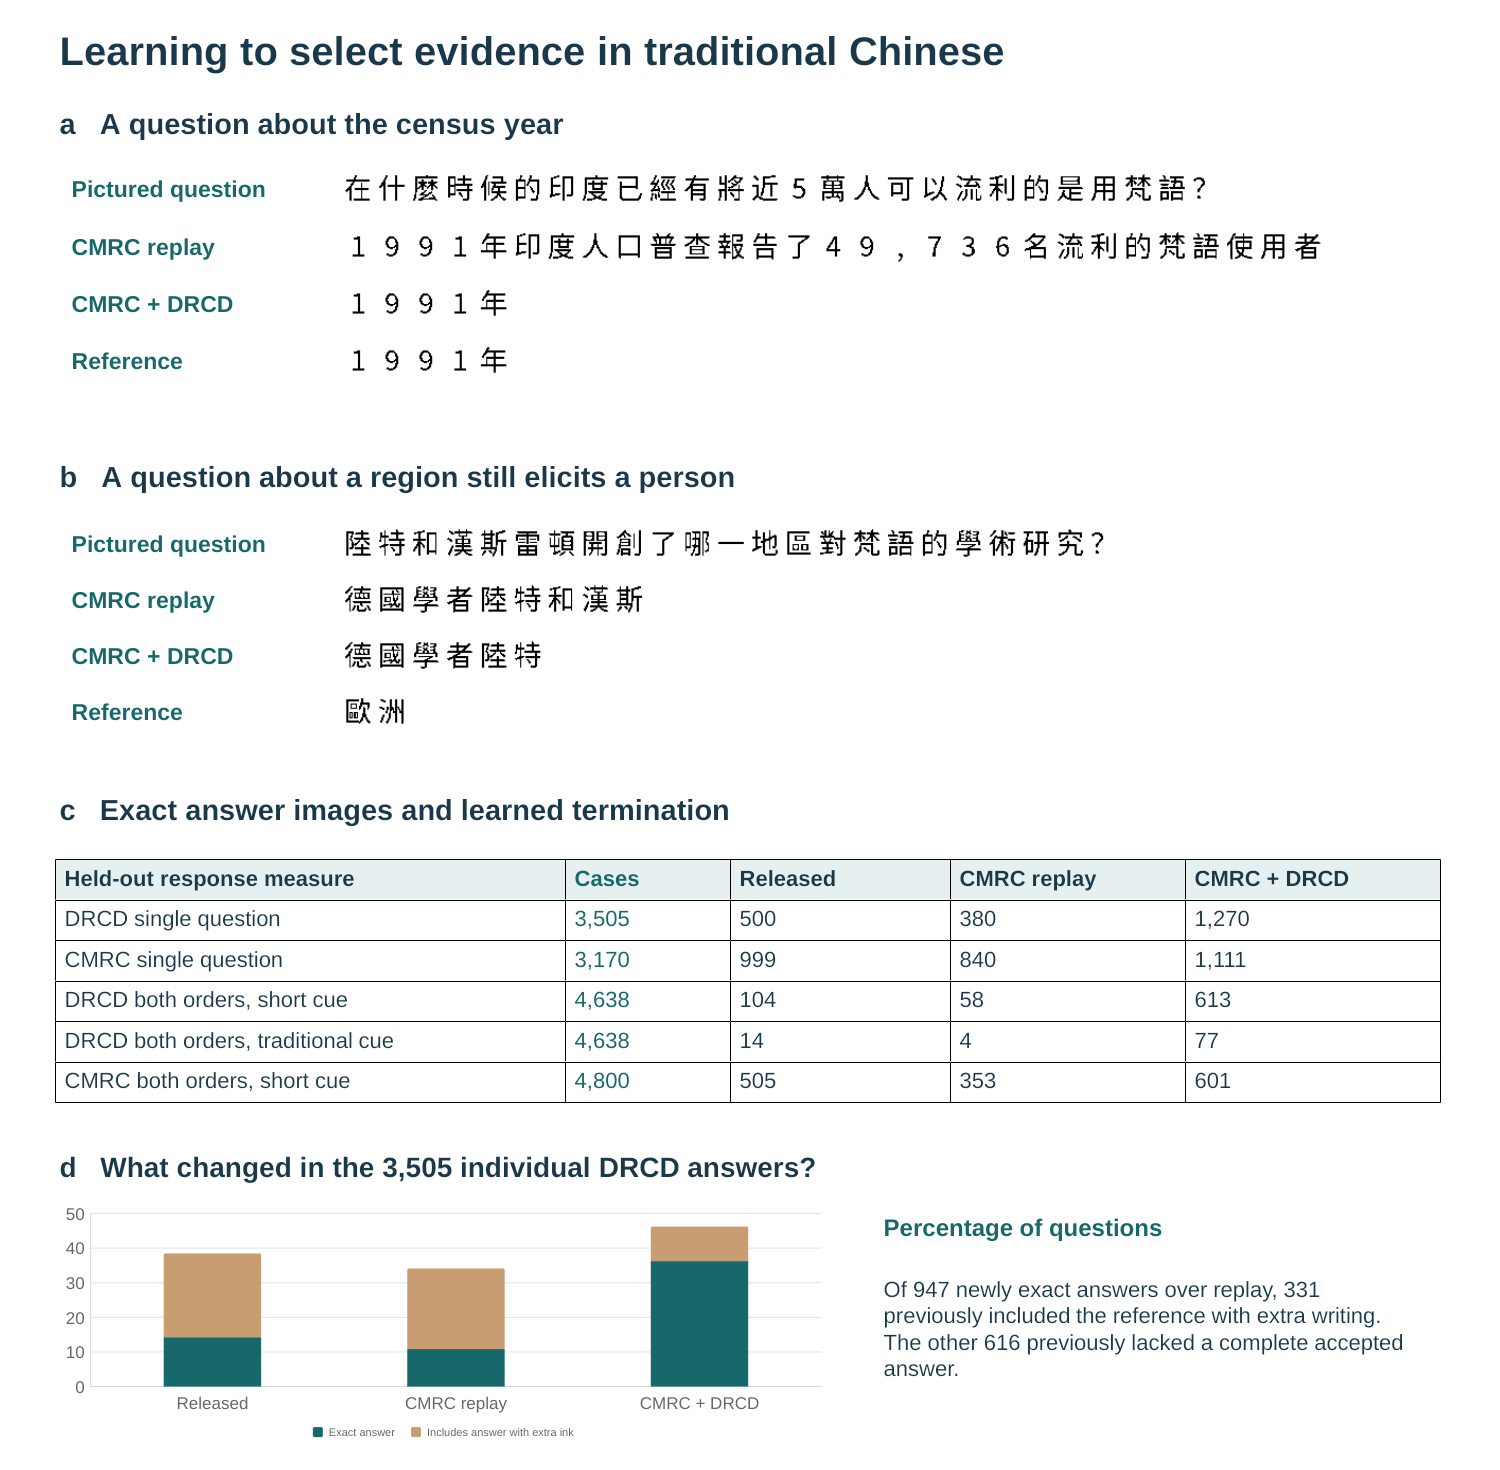
\includegraphics[width=.84\textwidth]{figures/Figure_74_traditional_passage.png}
\caption{\DIFaddFL{\textbf{Additional pictured questions improve extraction on two Chinese passage collections.} \textbf{a}, The first DRCD answer gained over matched replay. The reference is a year. Replay includes the year in a longer span. \textbf{b}, First remaining error. The question asks which region began academic research on Sanskrit. Both readers choose a person; the reference is Europe. All displayed strips contain the complete recorded images. \textbf{c}, Whole-image scores. For paired requests, both exchanged orders must terminate and match accepted references. The two DRCD instructions act on the same questions and passages. \textbf{d}, Percentage of individual DRCD outputs that equal an accepted answer or contain it with extra writing. Both categories require termination.}}
\label{fig:traditional-passage}
\end{figure*}
\clearpage
\begin{figure*}[p]
\centering

\includegraphics[width=.84\textwidth]{figures/Figure_75_composed_writer.png}
\caption{\DIFaddFL{\textbf{Learning to select a source span leaves missing content unwritten.} \textbf{a}, An independently authored question asks which script appears in a handout's right column. The reference is small-seal script. \textbf{b}, A second passage describes five bronze seals, two of which are sent away. Both examples show complete, unaltered decoded images from the final weights and lie outside the benchmark. \textbf{c}, Exact terminated references by physical accessibility, with all stops counted separately. Rotating each question to the next case leaves its original passage and scoring reference fixed. \textbf{d}, Exact missing glyphs with the reference segment history and writing action supplied. Both renderers share the same writing context. Their errors precede autonomous feedback.}}
\label{fig:composed-writer}
\end{figure*}
\begin{figure*}[p]
\centering

\includegraphics[width=.84\textwidth]{figures/Figure_76_bitmap_history.png}
\caption{\DIFaddFL{\textbf{Ordered glyph images predict Chinese spelling when the answer prefix is correct.}
\textbf{a}, Exact next-image choices with the correct action and antecedent answer segments supplied. The ordered and shuffled conditions use identical human answers and bitmap counts. \textbf{b}, Exact complete references and exact positions of missing glyphs when each system uses its own output history. The rotated-question condition uses the ordered index. \textbf{c}, The ordered writer's complete output on the two original prompts in Fig.~\ref{fig:composed-writer}, with their references. All printed response images are taken directly from CPU decoding. The conditional spelling gain does not produce either requested answer.}}
\label{fig:bitmap-history}
\end{figure*}
\begin{figure*}[p]
\centering
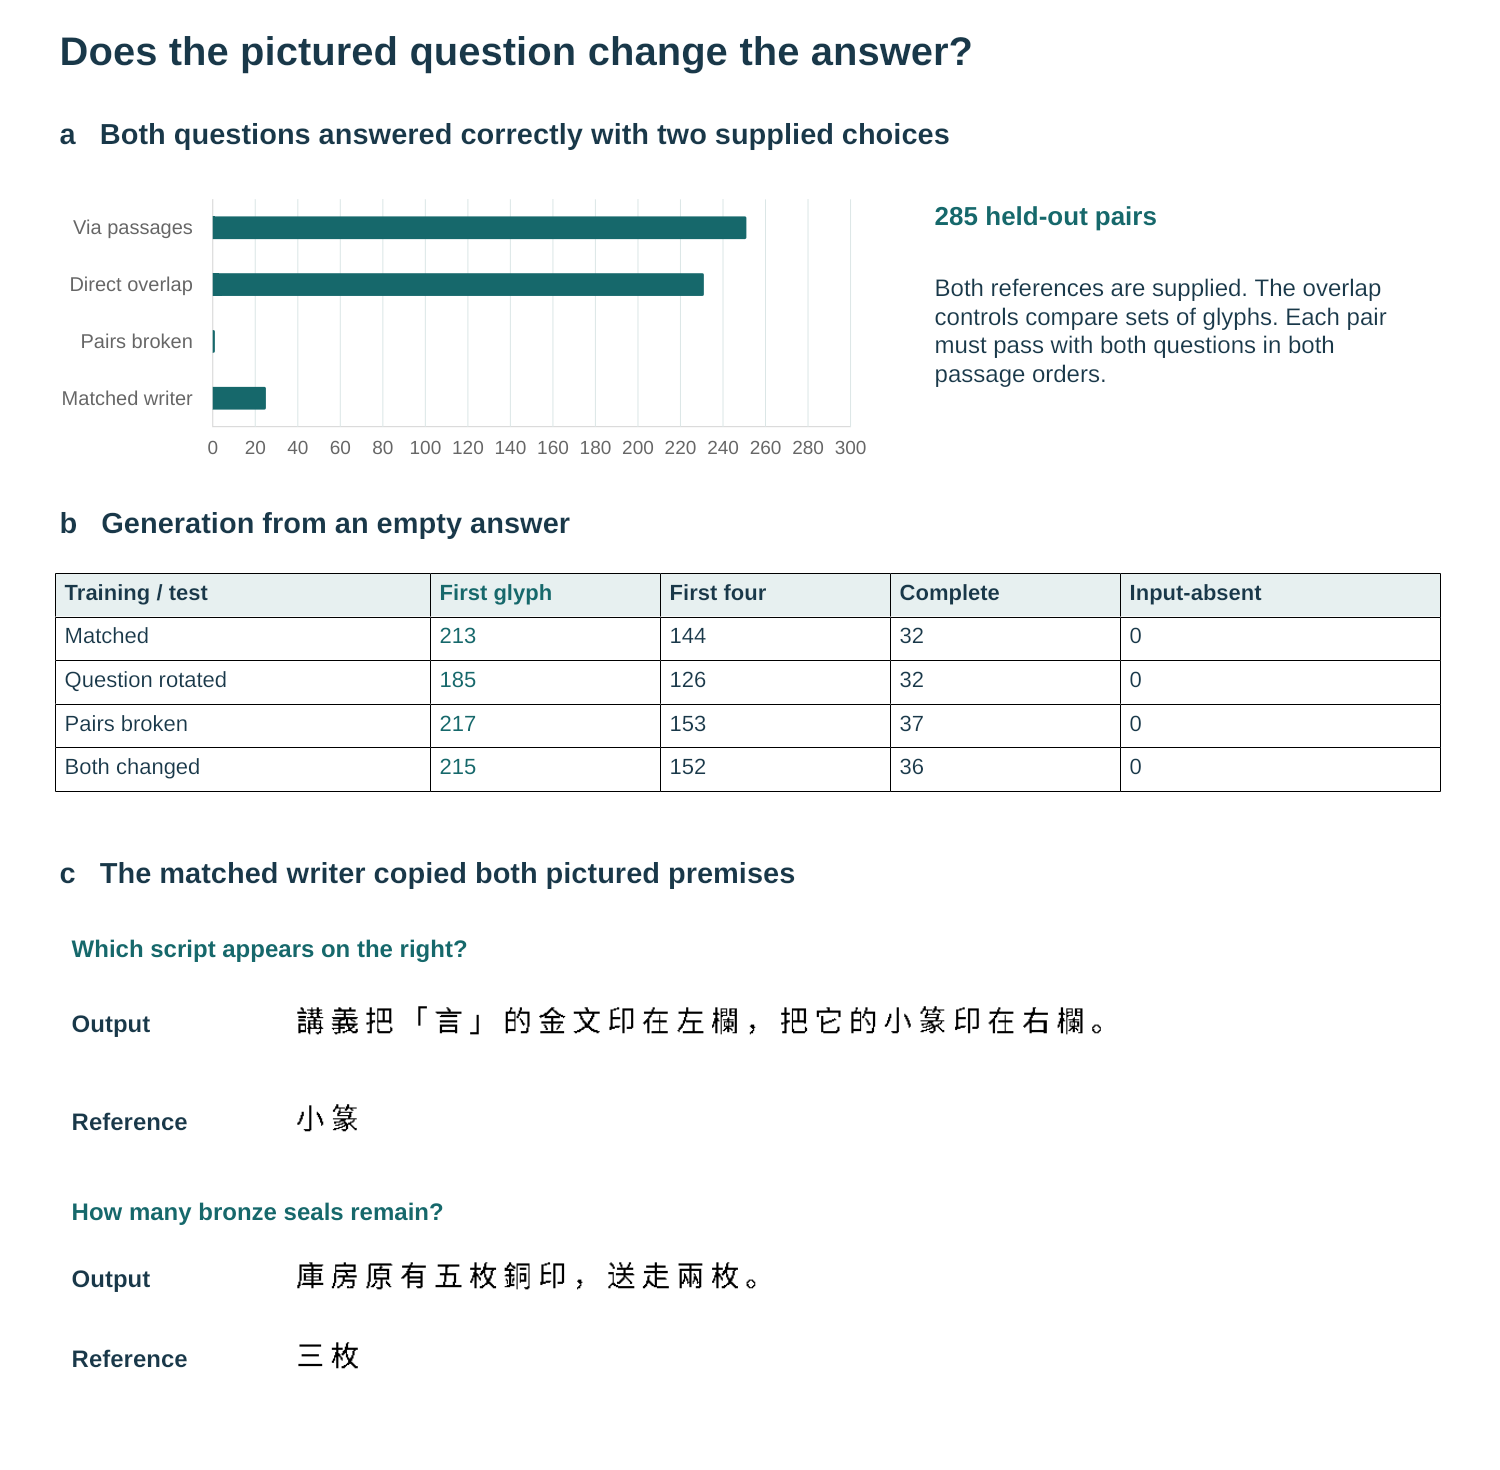
\includegraphics[width=.84\textwidth]{figures/Figure_77_grounded_glyph_writer.png}
\caption{\DIFaddFL{\textbf{Learning from paired questions and passages.}
\textbf{a}, Correct pairs when both candidate answers are supplied. Credit requires the writer to prefer each requested answer with the passages in either order. Direct overlap compares question and answer glyph sets. The second overlap rule uses the two passage regions. \textbf{b}, Exact agreements from an empty answer. The first three score columns use all 571 questions. The final column covers the 300 references containing a content glyph absent from both input images. Complete agreement includes the stop decision. \textbf{c}, The matched writer's complete outputs and the intended answers on the two original prompts in Fig.~\ref{fig:composed-writer}. Each output reproduces its passage pixel for pixel.}}
\label{fig:grounded-glyph-writer}
\end{figure*}
\begin{figure*}[p]
\centering
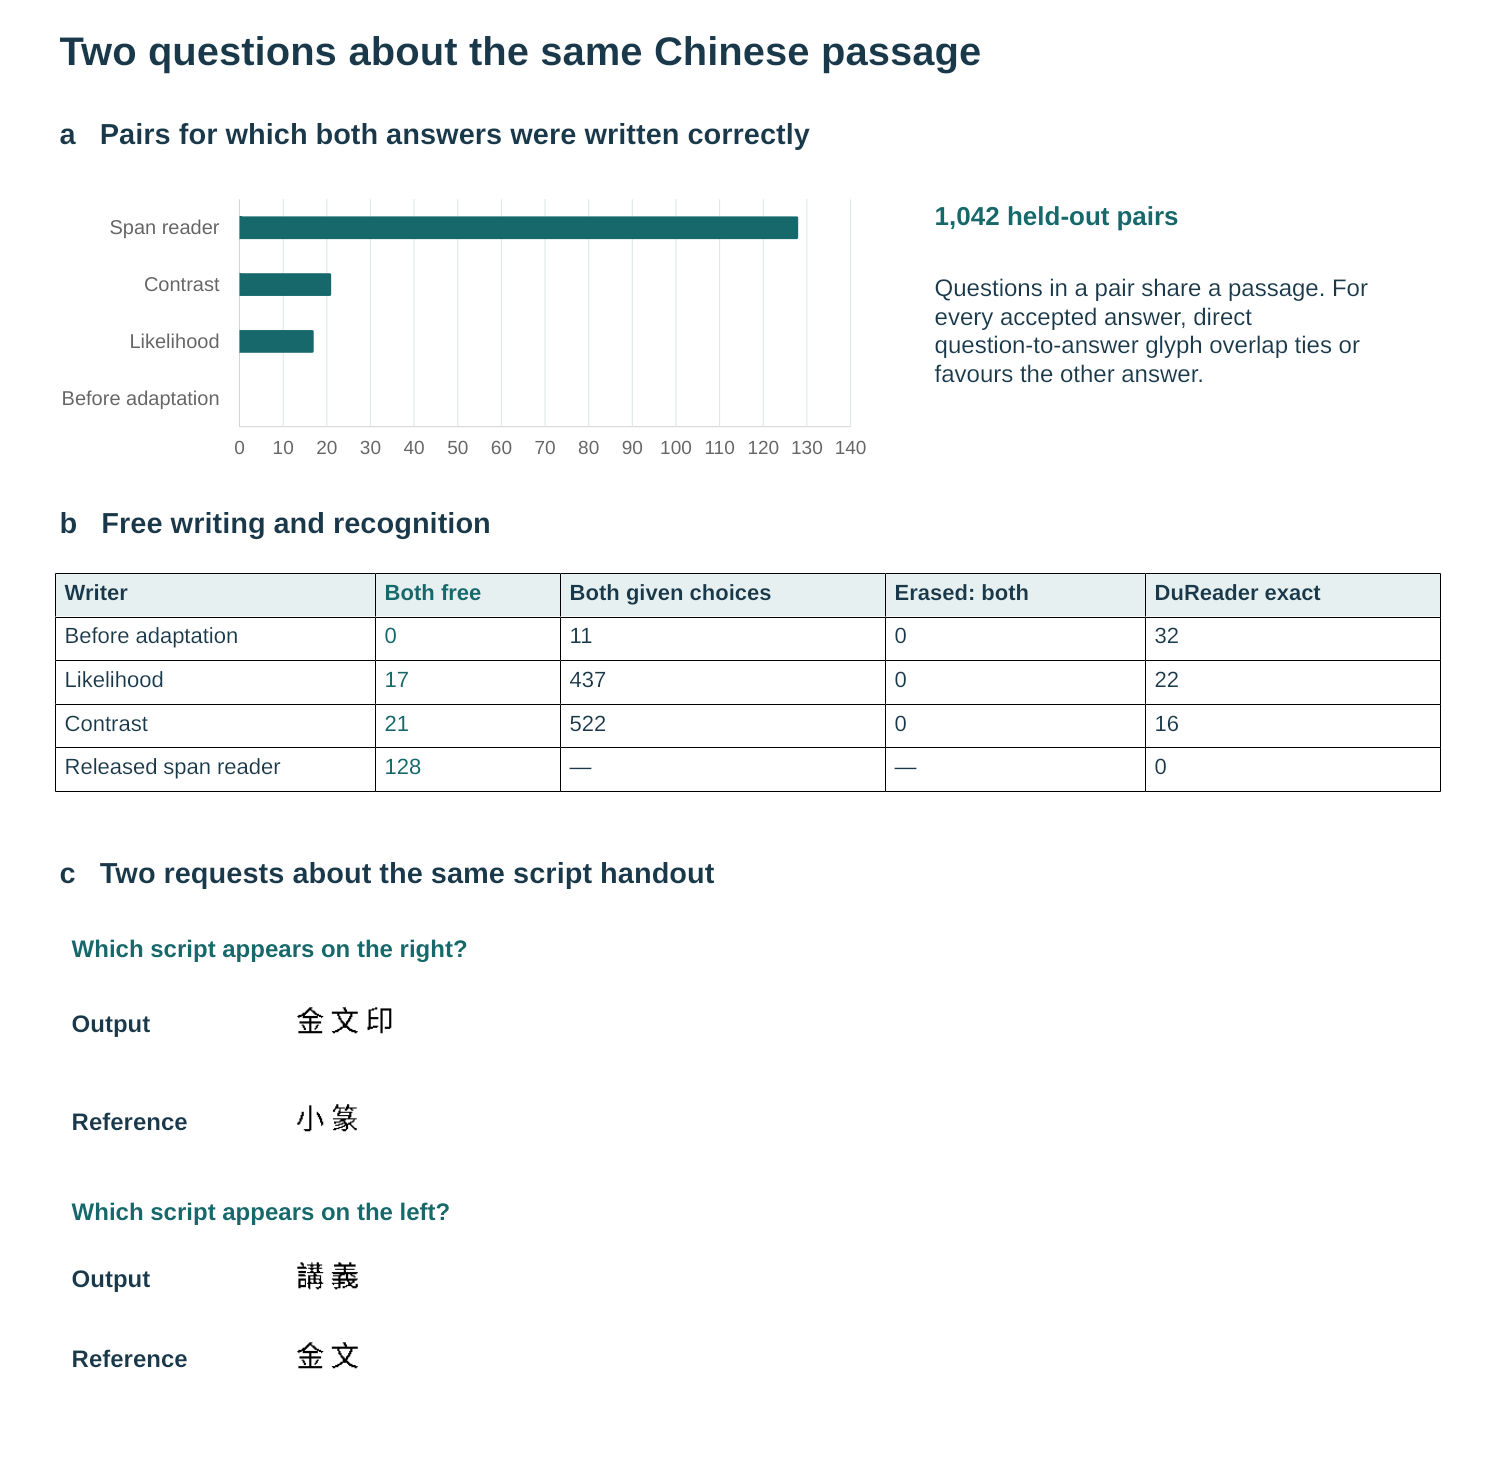
\includegraphics[width=.84\textwidth]{figures/Figure_78_same_passage_writer.png}
\caption{\DIFaddFL{\textbf{Answer recognition and generation in a common passage.}
\textbf{a}, Complete paired answers on 1,042 held-out question pairs. \textbf{b}, Both questions must succeed for paired credit. Supplied choices are compared by mean physical log likelihood. The DuReader column gives canonical stopped answers out of 571. The earlier span reader supplies a specialized comparison. \textbf{c}, The contrast writer's outputs on two author-written questions about the same handout, with the intended forms printed below. Both responses end with a learned stop.}}
\label{fig:same-passage-writer}
\end{figure*}
\begin{figure*}[p]
\centering

\includegraphics[width=.84\textwidth]{figures/Figure_79_general_entry_writer.png}
\caption{\DIFaddFL{\textbf{Historical forms from a shared image-stream writer.}
\textbf{a}, Attribution of the penultimate output cell on 1,136 standard questions about 142 two-entry cards. Each card contains two different historical stages for each headword. \textbf{b}, Exact, stopped outputs across dictionary and modern passage tasks. The located condition adds a pictured-headword matching rule to the matched writer. New wordings were written independently by a local language model. \textbf{c}, Actual responses to two typed questions about the same one-entry card. Both responses match the lexical fact and archived form. The headword and facts were seen in training with different historical exemplars. \textbf{d}, First held-out response in corpus order that copied a distractor form from the requested stage. The second output applies the locator with identical weights. The reference uses the archived form of the requested headword.}}
\label{fig:general-entry-writer}
\end{figure*}
\begin{figure*}[p]
\centering
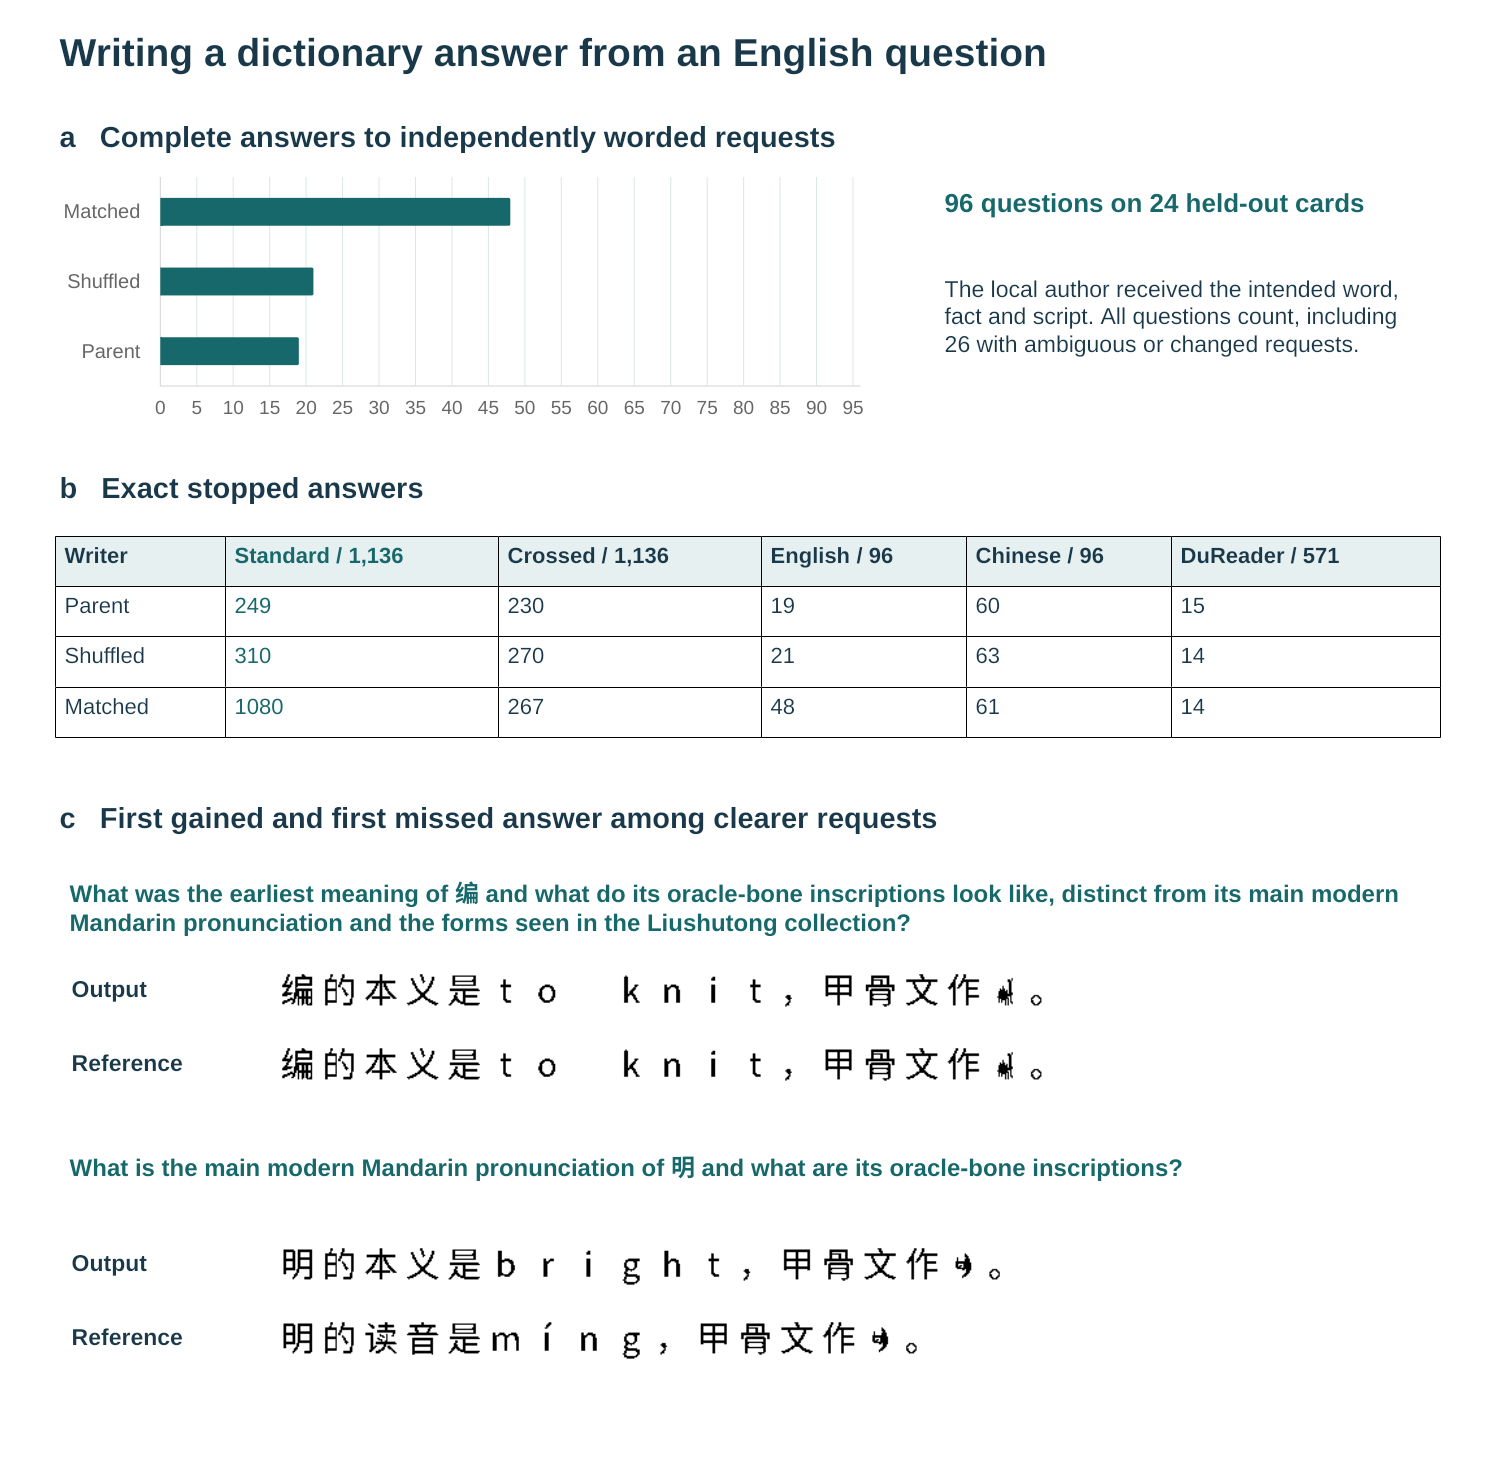
\includegraphics[width=.84\textwidth]{figures/Figure_80_english_request_writer.png}
\caption{\DIFaddFL{\textbf{English questions about pictured Chinese entries.}
\textbf{a}, Correct stopped answers on 96 English requests written by a separate local model. \textbf{b}, The standard and crossed English constructions each cover the same 1,136 targets. Four crossed requests for a headword contain identical multisets of glyphs. The Chinese column uses independently written Chinese questions. Dictionary scores use the visible-headword locator. \textbf{c}, Original response and source-reference images for the first gain over initialization and the first miss in corpus order among the 70 clearer requests.}}
\label{fig:english-request-writer}
\end{figure*}
\begin{figure*}[p]
\centering
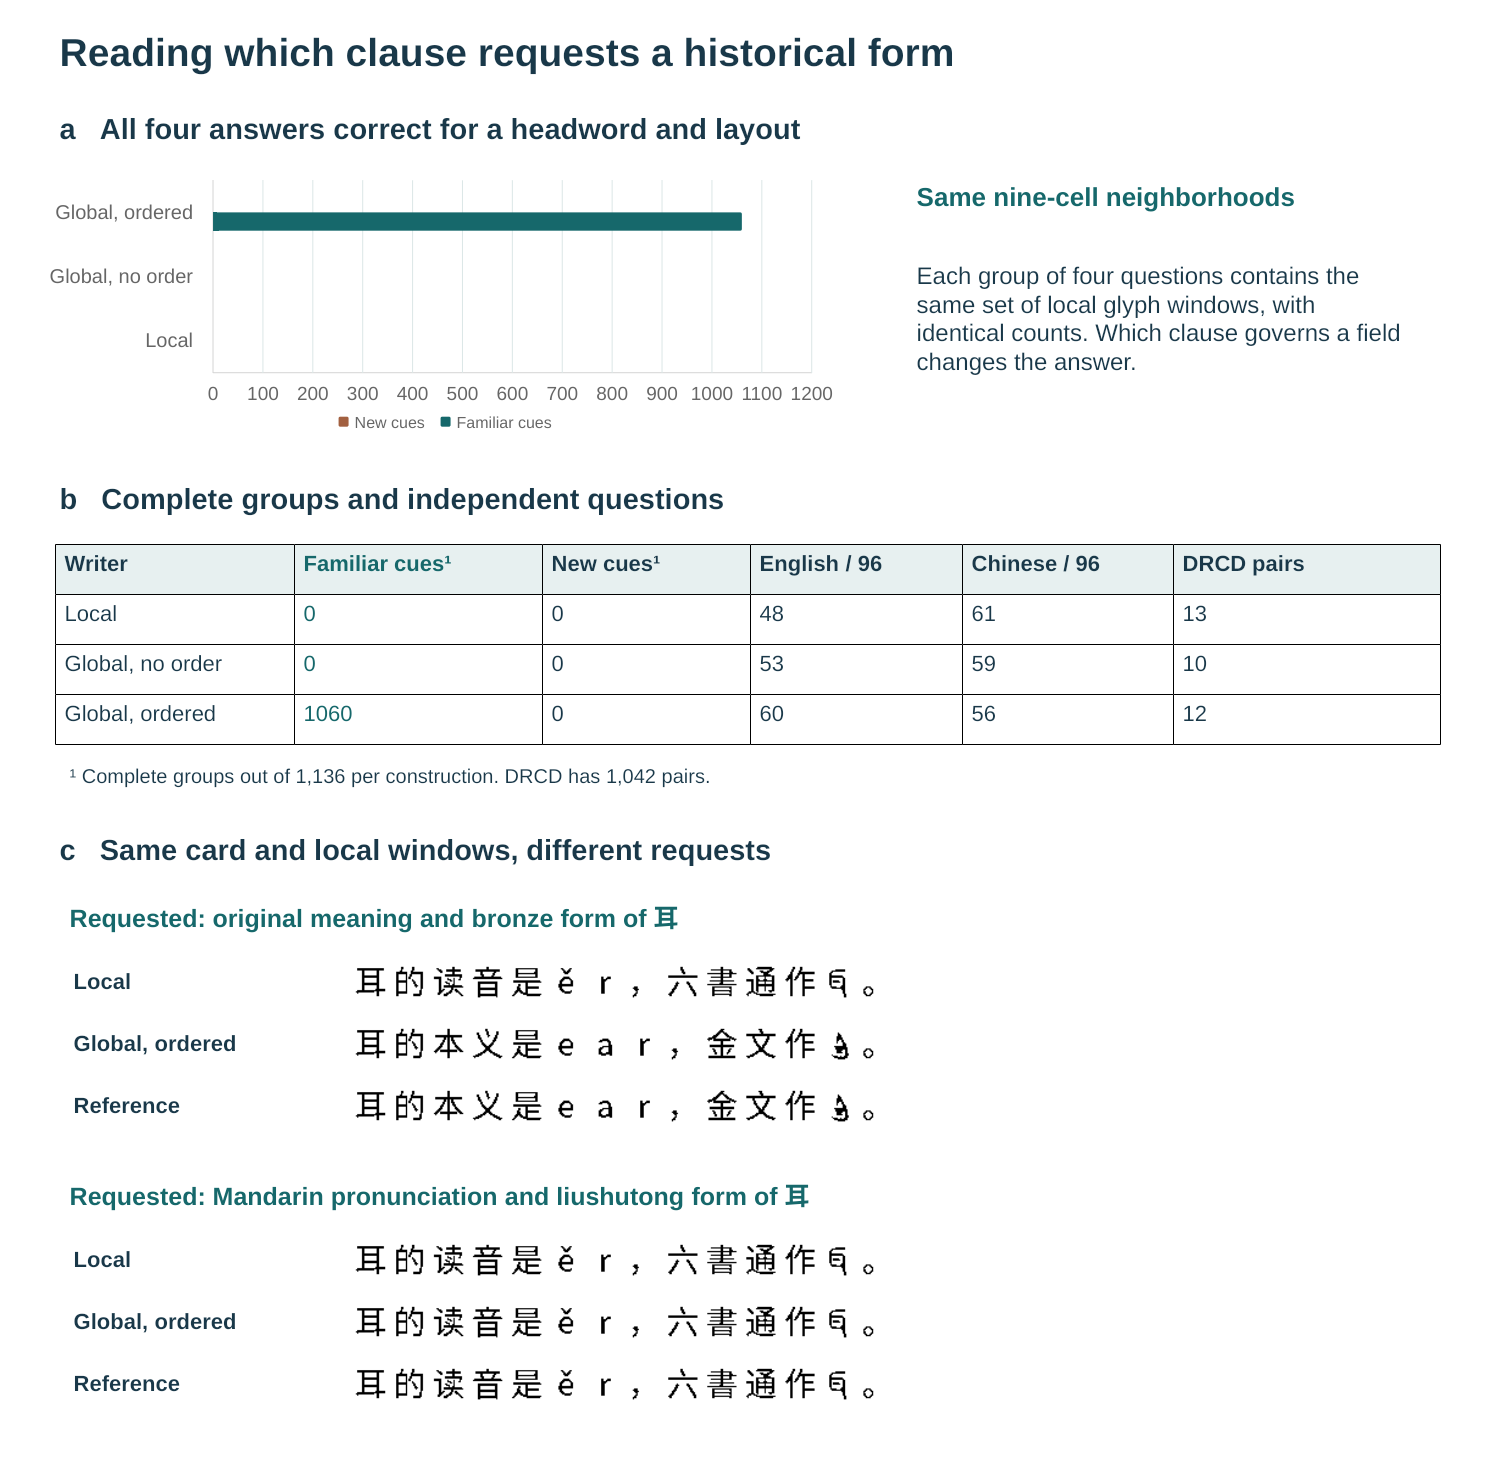
\includegraphics[width=.84\textwidth]{figures/Figure_81_scoped_request_writer.png}
\caption{\DIFaddFL{\textbf{Reading order distinguishes questions with identical local neighborhoods.}
\textbf{a}, Correct answers to all four requests in a headword--layout group, out of 1,136 groups per test construction. The local writer and the two global-attention writers share the same physical output format. \textbf{b}, The English and Chinese columns give complete responses on 96 independent requests per language. The DRCD column requires both answers to be correct on a shared passage. \textbf{c}, Outputs for the first held-out headword in the first layout. The field and script change together between the two displayed requests. Local and ordered outputs and both source-listed reference images are shown at their emitted resolution.}}
\label{fig:scoped-request-writer}
\end{figure*}
\begin{figure*}[p]
\centering
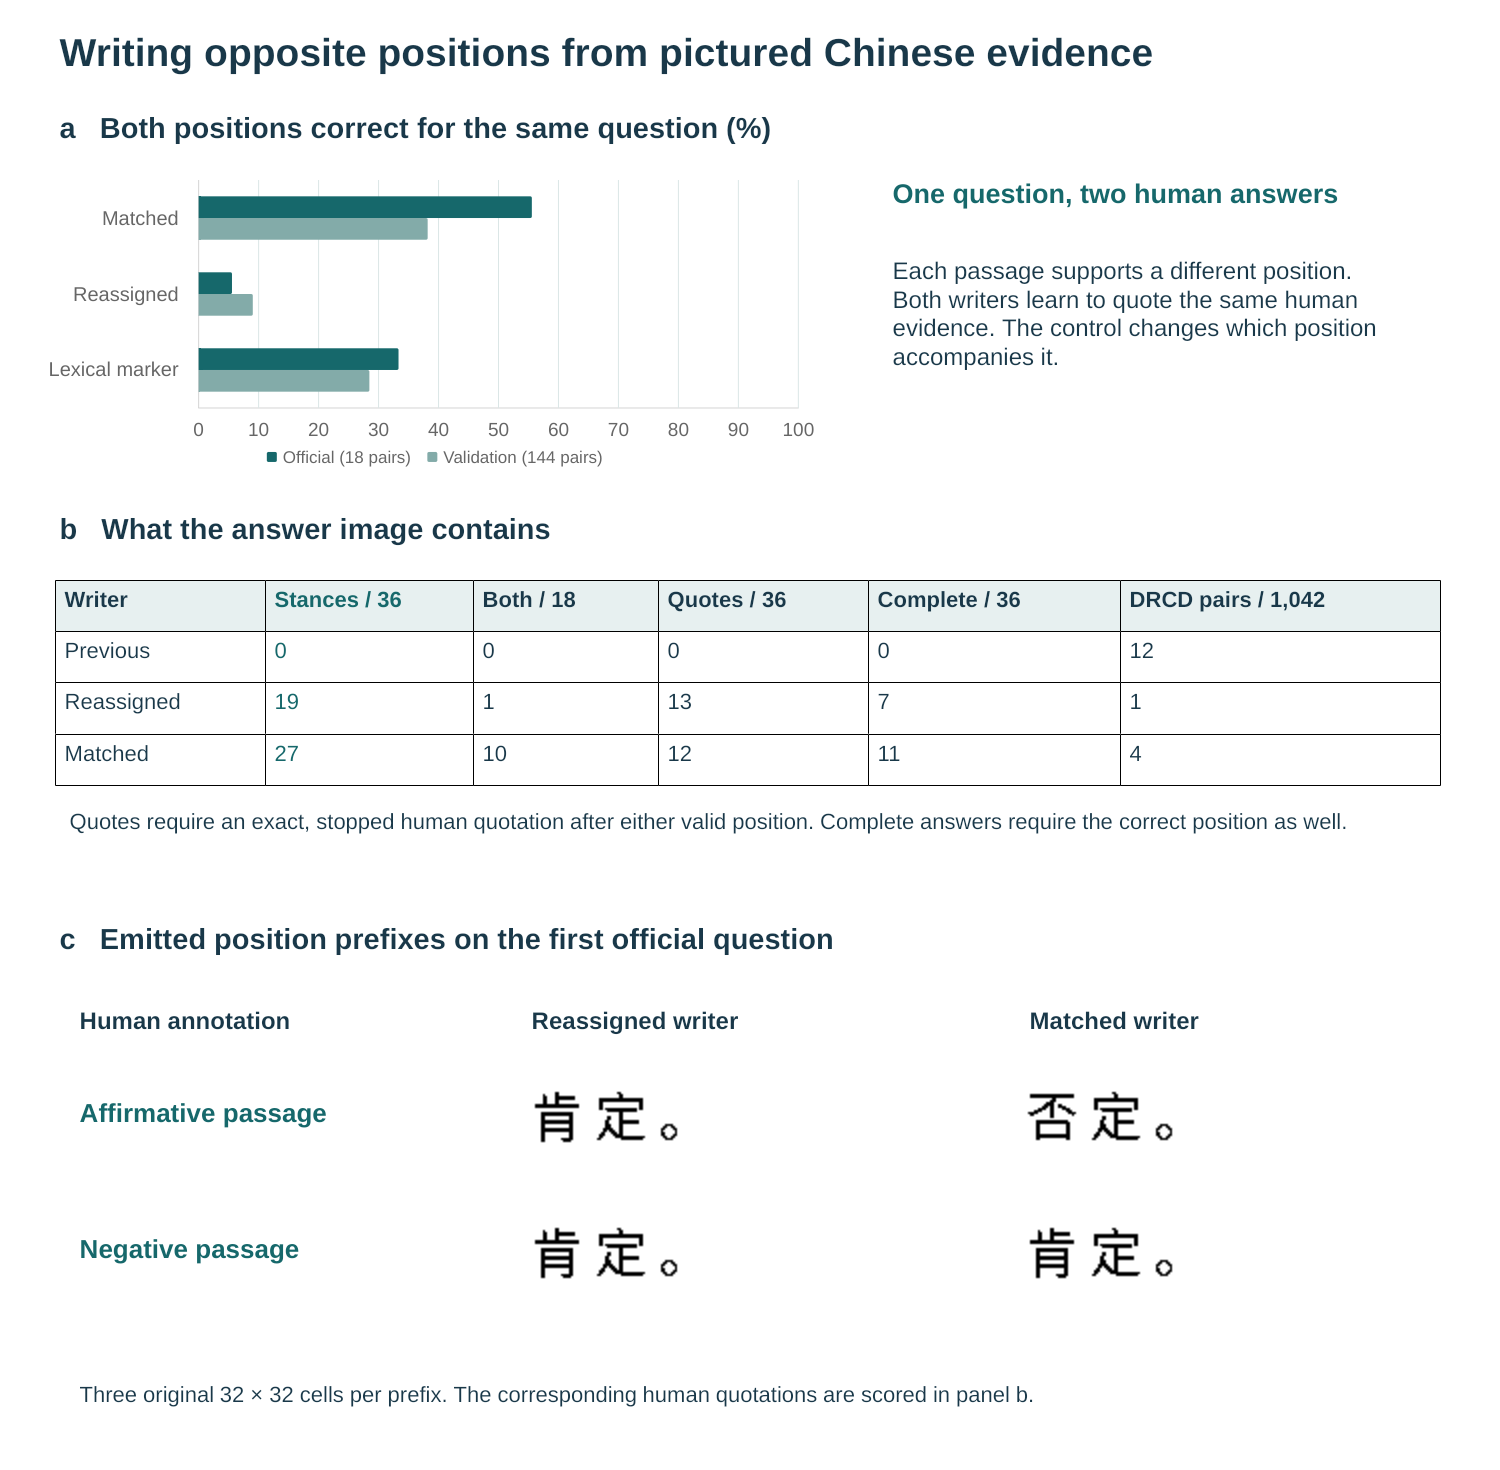
\includegraphics[width=.84\textwidth]{figures/Figure_82_paired_stance_writer.png}
\caption{\DIFaddFL{\textbf{Opposing evidence can change the stance that the model writes.}
\textbf{a}, Percentage of question pairs for which both written positions agree with the human annotations, on the validation and official cohorts. \textbf{b}, Stance, human quotation and complete stopped answer counts on 36 official responses. The last column measures retention on previously evaluated traditional Chinese questions. \textbf{c}, The first three emitted bitmap cells on each side of the first official pair. They label an affirmative or negative position before the model writes the quotation. The passages and human quotations remain in the local research corpus.}}
\label{fig:paired-stance-writer}
\end{figure*}
\begin{figure*}[p]
\centering

\includegraphics[width=.84\textwidth]{figures/Figure_83_visual_inference_writer.png}
\caption{\DIFaddFL{\textbf{Visual inference and restoration from original Chinese text.}
\textbf{a}, Percentage of complete stopped image responses matching the OCNLI relation sentence or the human text removed from the claim. The missing-ink subset requires at least one target glyph unavailable in the displayed inputs.
\textbf{b}, Official development counts. Triples contain three claims with different relations to the same premise. The local controls use visual unigram, bigram and overlap features for decisions and neighboring-glyph counts for missing text.
\textbf{c}, The model's complete outputs on the first two newly written restoration examples. Changing the drink in the passage changes the warranted missing glyph. The first two columns show the input rasters.}}
\label{fig:visual-inference-writer}
\end{figure*}
\begin{figure*}[p]
\centering
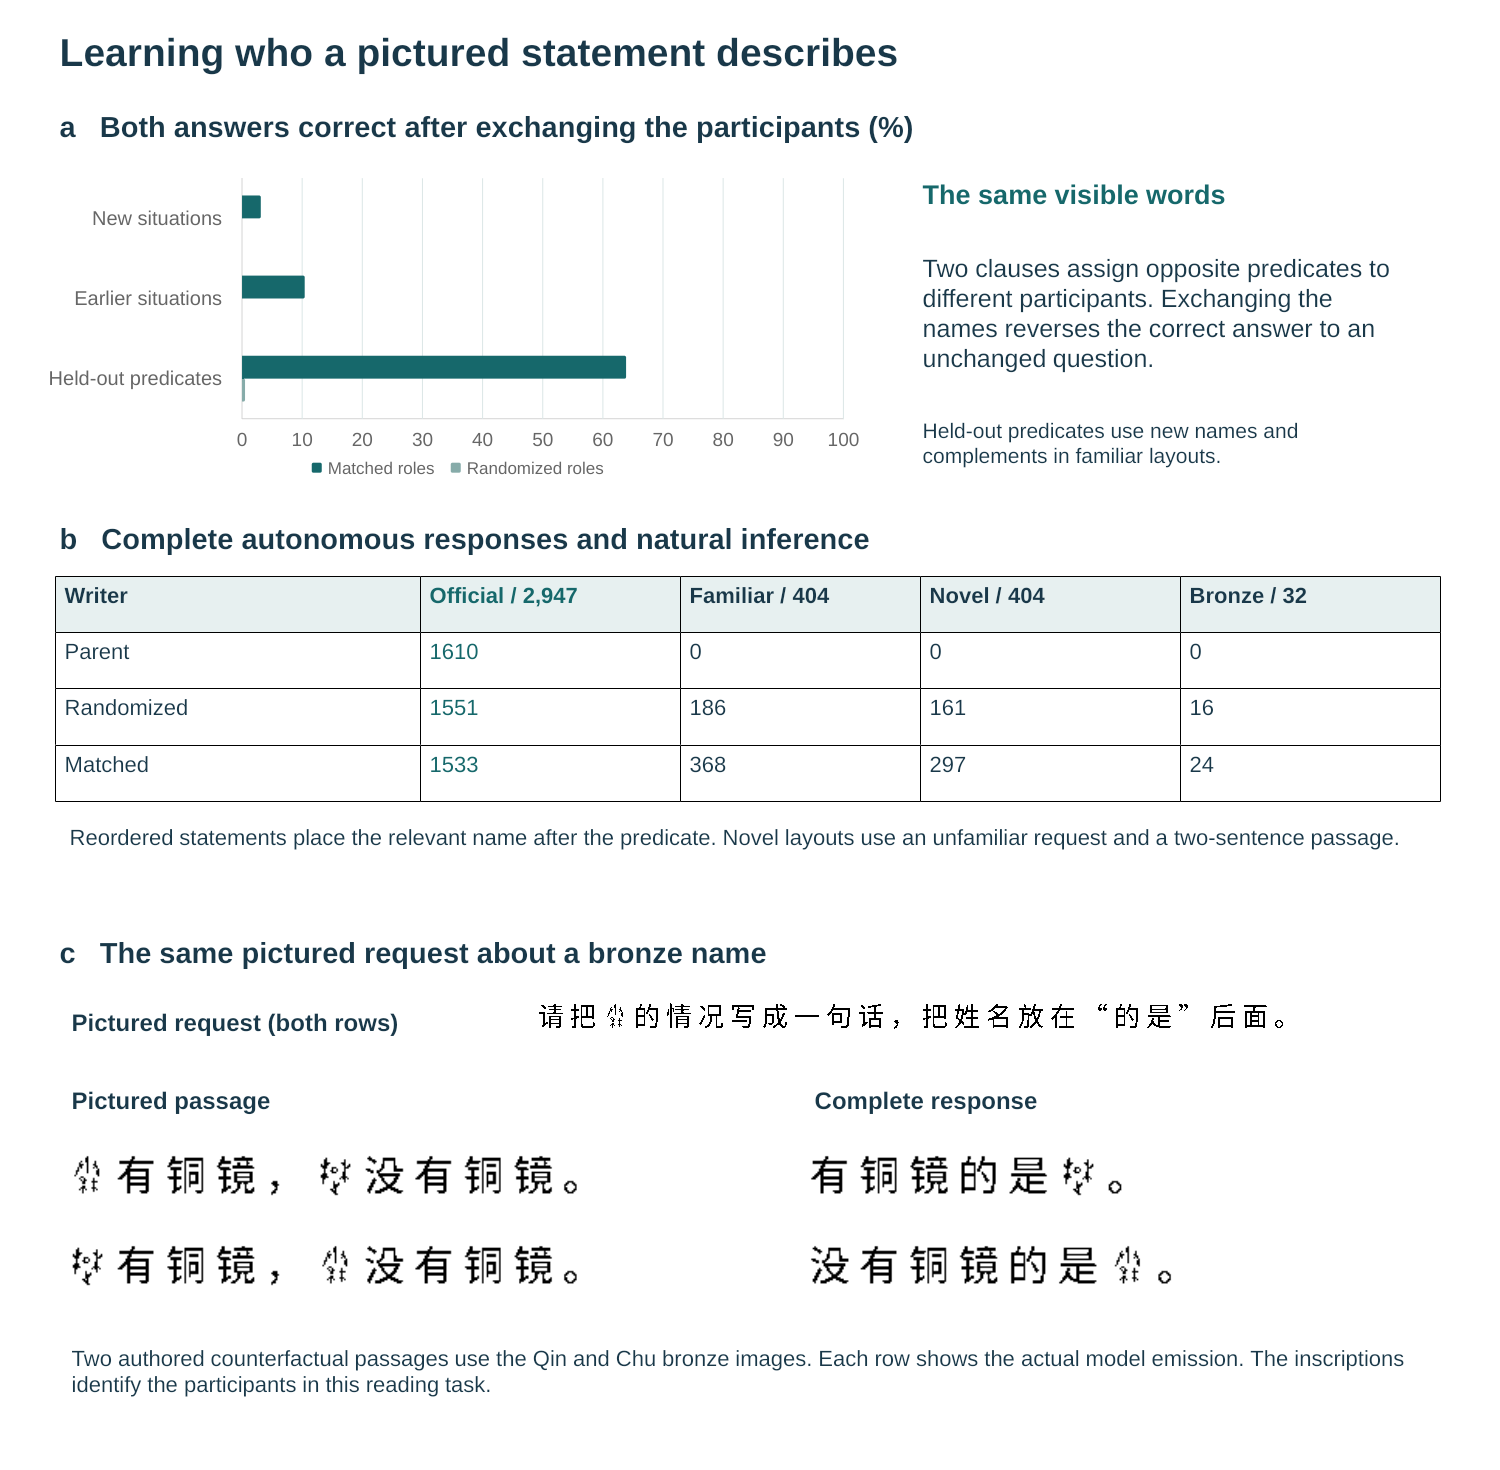
\includegraphics[width=.84\textwidth]{figures/Figure_84_visual_role_writer.png}
\caption{\DIFaddFL{\textbf{Writing about participants after a visual role exchange.}
\textbf{a}, Both judgments must be correct when the two participants change places in the source and the pictured claim stays fixed. Held-out predicates use previously unseen complements and names in familiar layouts. The two other sets contain independently worded situations.
\textbf{b}, Exact stopped answers for the unmodified parent and the two fitted writers. Reordered writing requires a complete predicate, complement and name.
\textbf{c}, The same pictured question asks about Qin. Each displayed passage assigns the bronze images for Qin and Chu opposite properties. The examples are counterfactual reading tests. The first response ends with Chu where Qin is required; the second correctly ends with Qin.}}
\label{fig:visual-role-writer}
\end{figure*}
\begin{figure*}[p]
\centering

\includegraphics[width=.84\textwidth]{figures/Figure_85_inverse_role_writer.png}
\caption{\DIFaddFL{\textbf{Following an unnamed participant in a pictured question.}
\textbf{a}, Exact stopped answers for 387 human-written DRCD questions using the complete passage or the sentence with the highest visual glyph overlap with the question. Both adapted writers received the original single-question supervision. The randomization changes the additional competing assignments.
\textbf{b}, Whole images scored on two-name bronze and four-name historical identification, an unfamiliar printed description layout, and natural DuReader responses.
\textbf{c}, The source says that Qin has a bronze mirror and Chu lacks one. Asked who has the mirror (upper row) and who lacks it (lower row), the writer returns the same attested Qin image twice.
\textbf{d}, Asked who invented the Jiguang biscuit, the writer returns Matsu. The recorded answer is Qi Jiguang. The output is the original model image from the first wrong-first-glyph question with an identifiable source span in cohort order.}}
\label{fig:inverse-role-writer}
\end{figure*}
\begin{figure*}[p]
\centering
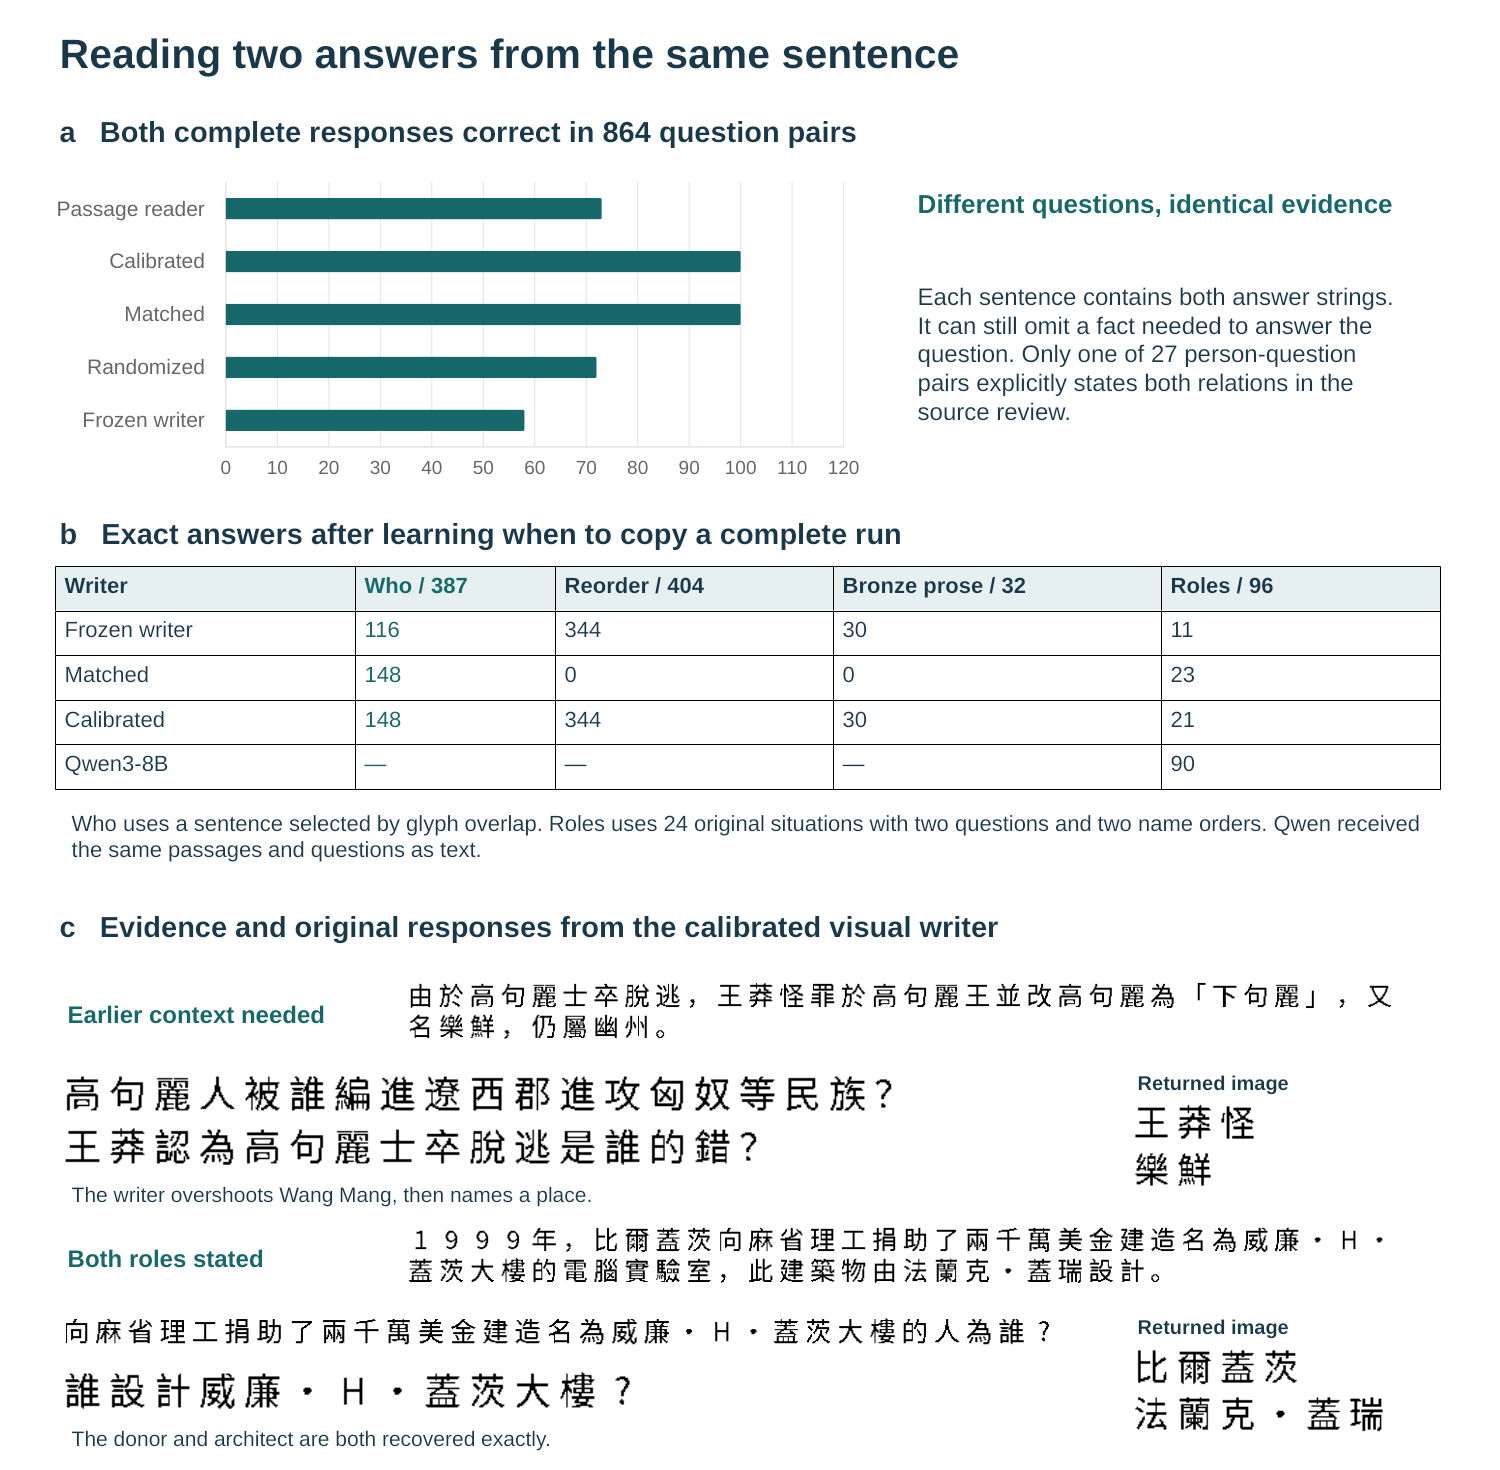
\includegraphics[width=.84\textwidth]{figures/Figure_86_shared_sentence_writer.png}
\caption{\DIFaddFL{\textbf{Reading and composing answers about different participants.}
\textbf{a}, Both answers must match accepted human references as complete stopped images for the same pictured sentence. The extra paired training examples keep their assignments or exchange them at random.
\textbf{b}, Counts before and after calibrating the choice of output action. The role questions test 24 new situations under name exchange. The text reference is a local Qwen3-8B model.
\textbf{c}, Original images for the first two person-question pairs in fixed order. In the upper example the writer extends the first name by one glyph and gives an alternate place name for the second. In the lower example the questions ask for the donor and architect of the Gates building. Both complete outputs agree with the recorded names.}}
\label{fig:shared-sentence-writer}
\end{figure*}
\begin{figure*}[p]
\centering
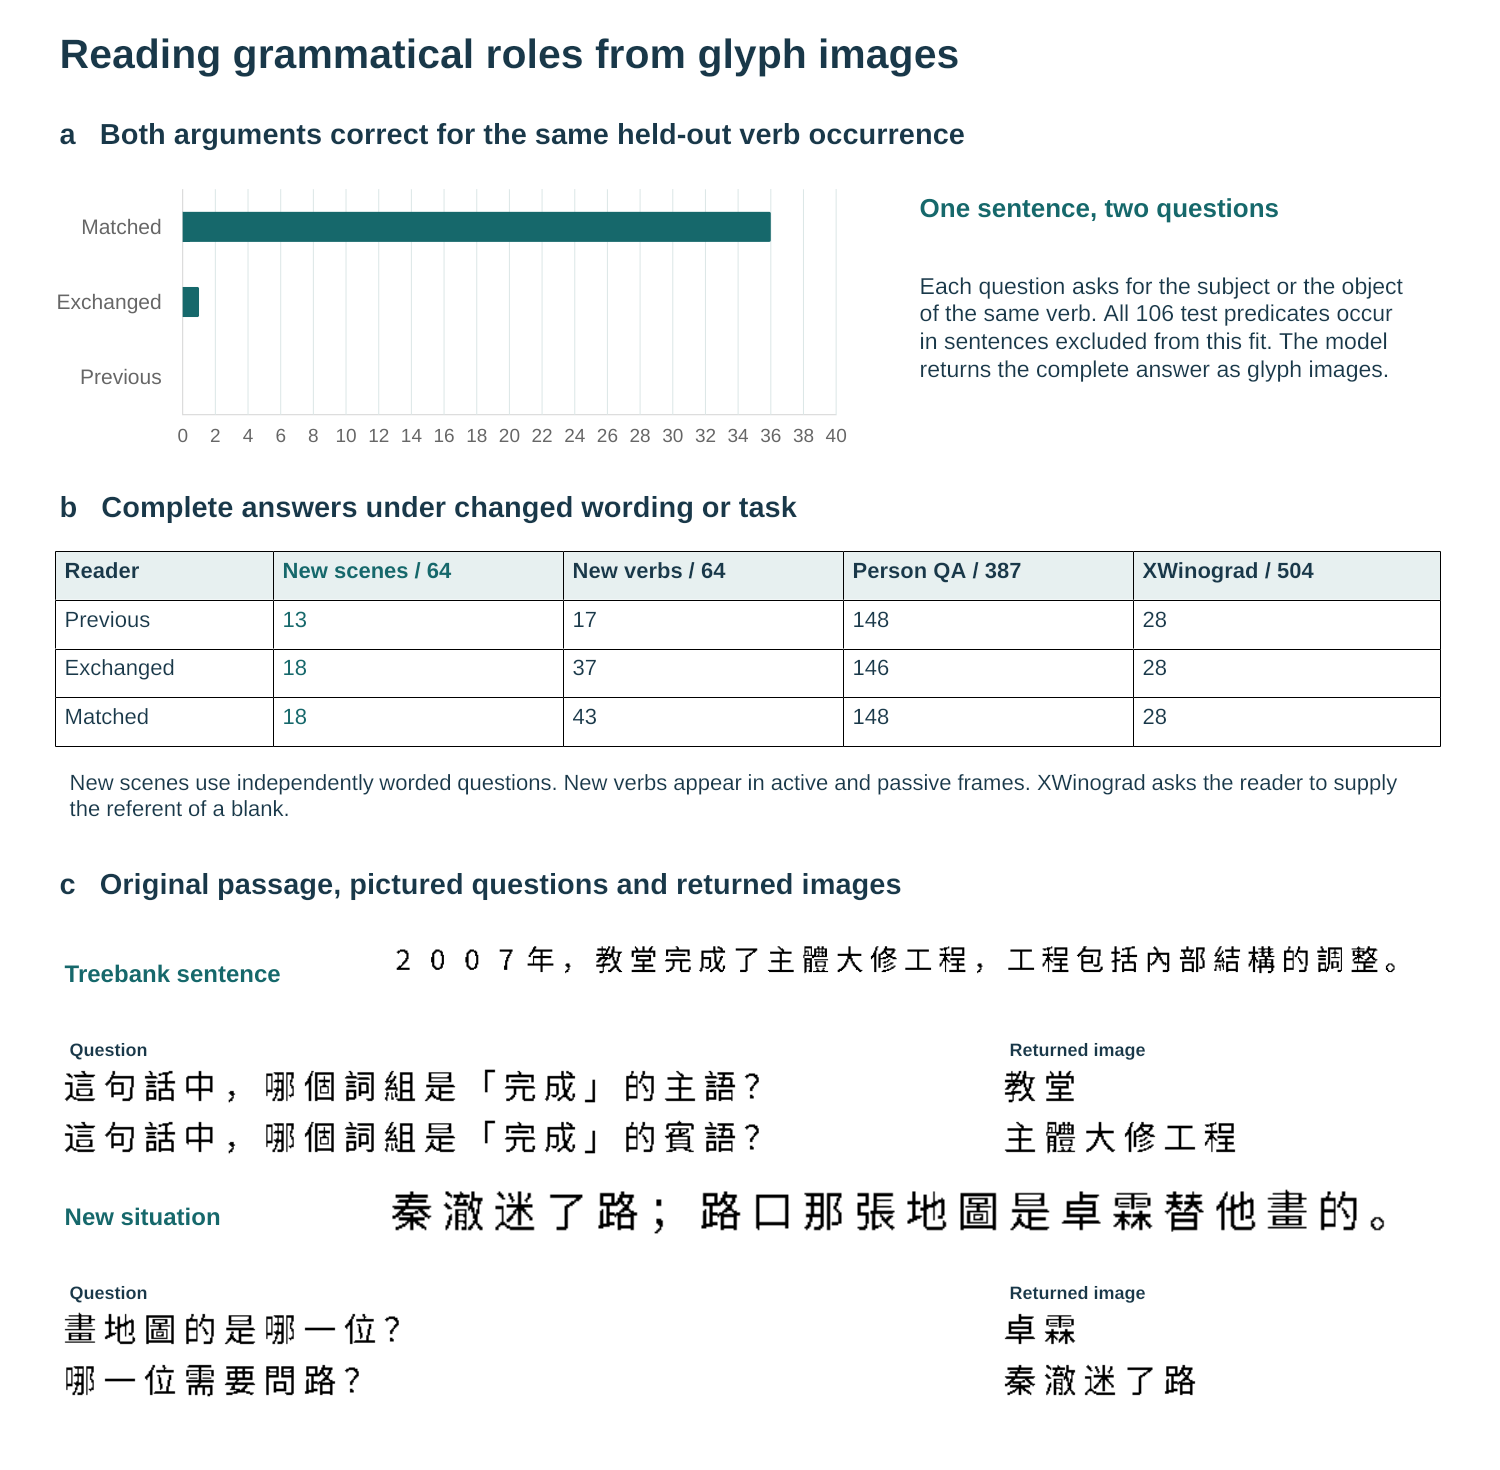
\includegraphics[width=.84\textwidth]{figures/Figure_87_pictured_participant_reader.png}
\caption{\DIFaddFL{\textbf{Learning to read a verb's two arguments in pictured Chinese.}
\textbf{a}, Count of test predicates for which both complete stopped answer images match the annotated subject and object. Both arms saw identical pictures. The control exchanged role targets during training.
\textbf{b}, Individual exact responses on new situations, held-out verbs in controlled sentence frames, natural person questions with glyph-overlap sentence selection, and external referent completion with answer options withheld.
\textbf{c}, The first completely correct matched-reader test pair in Chinese GSD order (fifth eligible predicate) and the first independently written map-drawing situation in fixed order. The upper responses identify the church and the principal renovation project. The lower responses give the map maker's name, then a clause beginning with the lost person's name. Images are original inputs and complete returned glyphs. The treebank sentence and derived question targets are from Chinese GSD r2.16, CC BY-SA 4.0.}}
\label{fig:pictured-participant-reader}
\end{figure*}
\begin{figure*}[p]
\centering
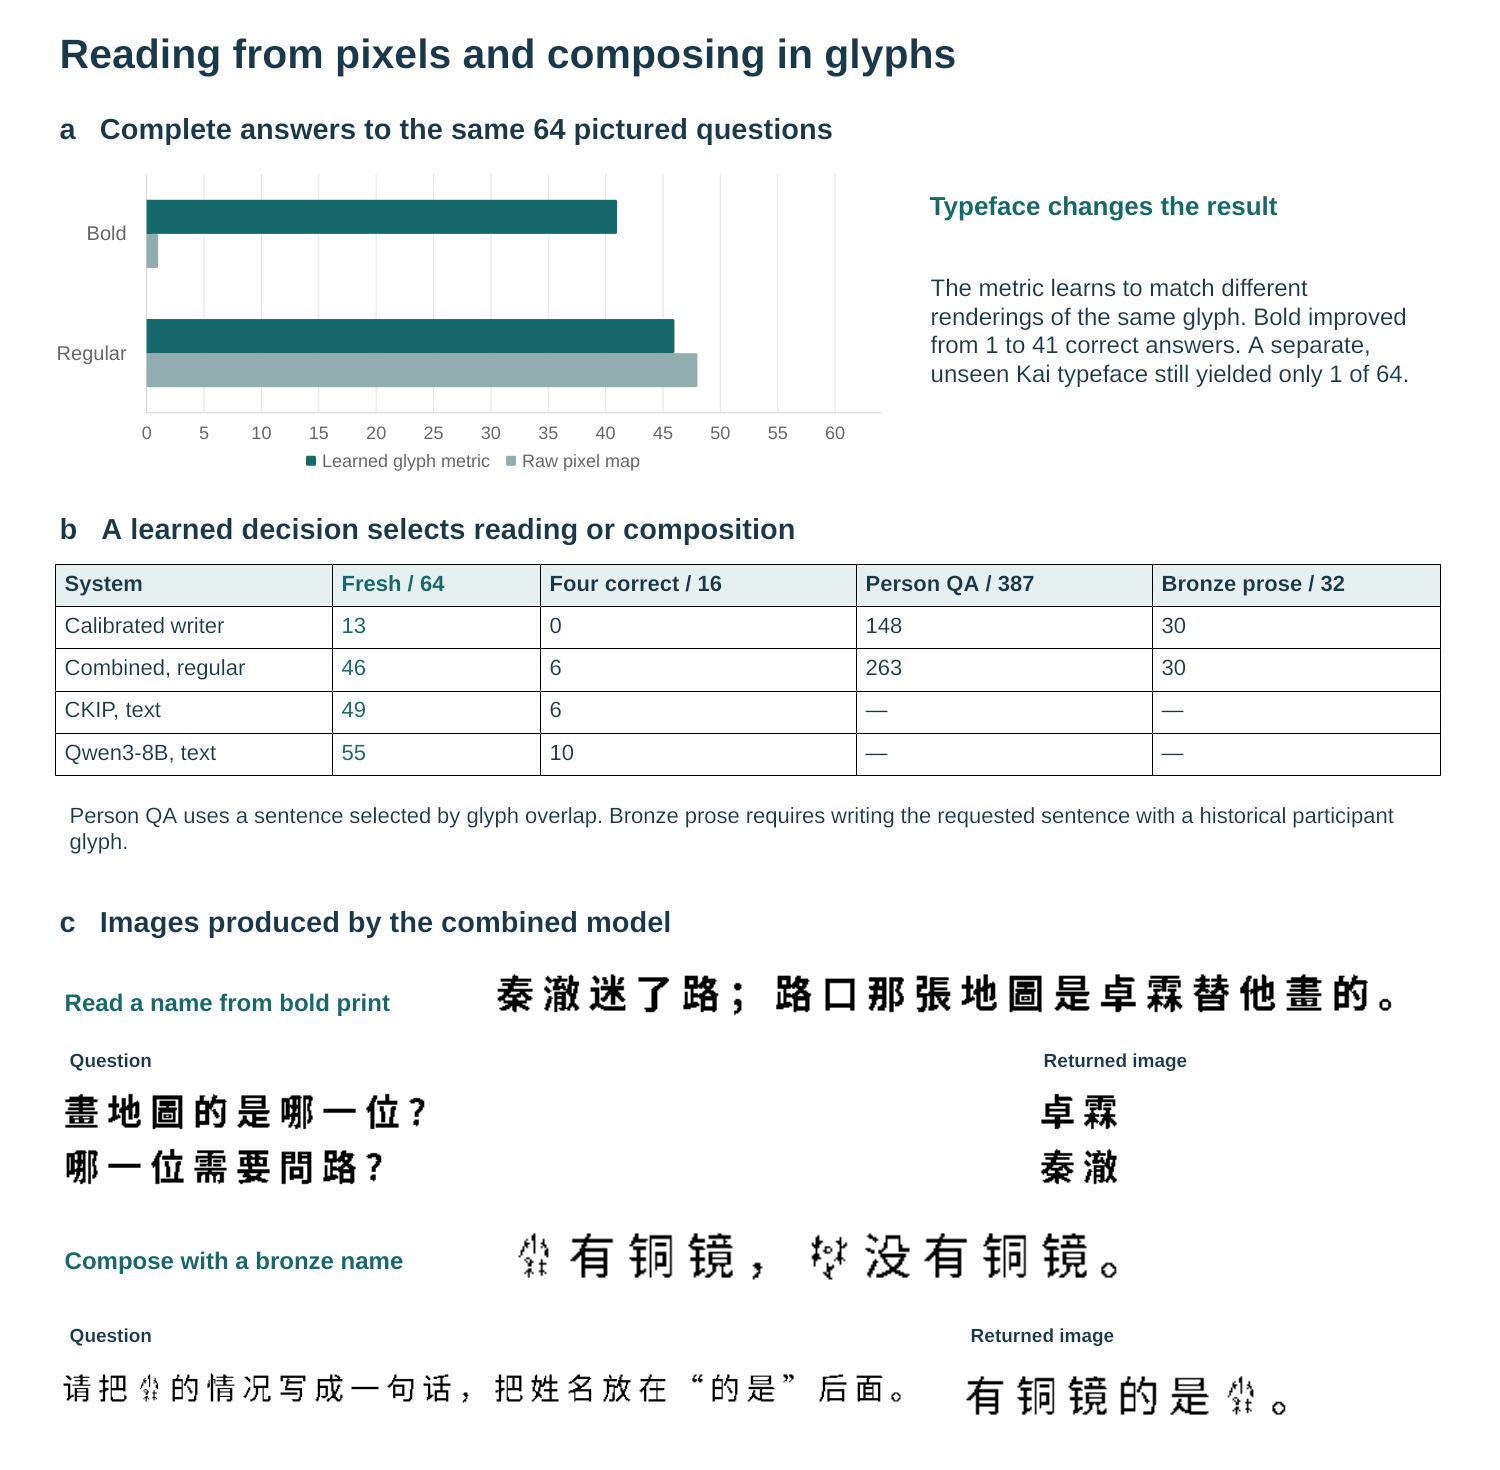
\includegraphics[width=.84\textwidth]{figures/Figure_88_font_invariant_reader.png}
\caption{\DIFaddFL{\textbf{Continuous visual reading and recurrent glyph writing.}
\textbf{a}, Exact answer images for the same 64 questions in regular and held-out bold print. A raw-pixel regression and a learned visual metric supply continuous inputs to the same pretrained contextual reader.
\textbf{b}, Complete-answer counts. The frozen gate selects the contextual reader or the recurrent writer. Text references use the original questions and passages. Dashes indicate comparisons not measured in that cohort.
\textbf{c}, The first new scene asks who drew a map and who needed directions. The two original bold answer images give the correct names. The first historical description requires a rearranged statement carrying a bronze glyph. The recurrent writer composed the complete reference. No display font substitutes for the returned historical image.}}
\label{fig:font-invariant-reader}
\end{figure*}
\begin{figure*}[p]
\centering
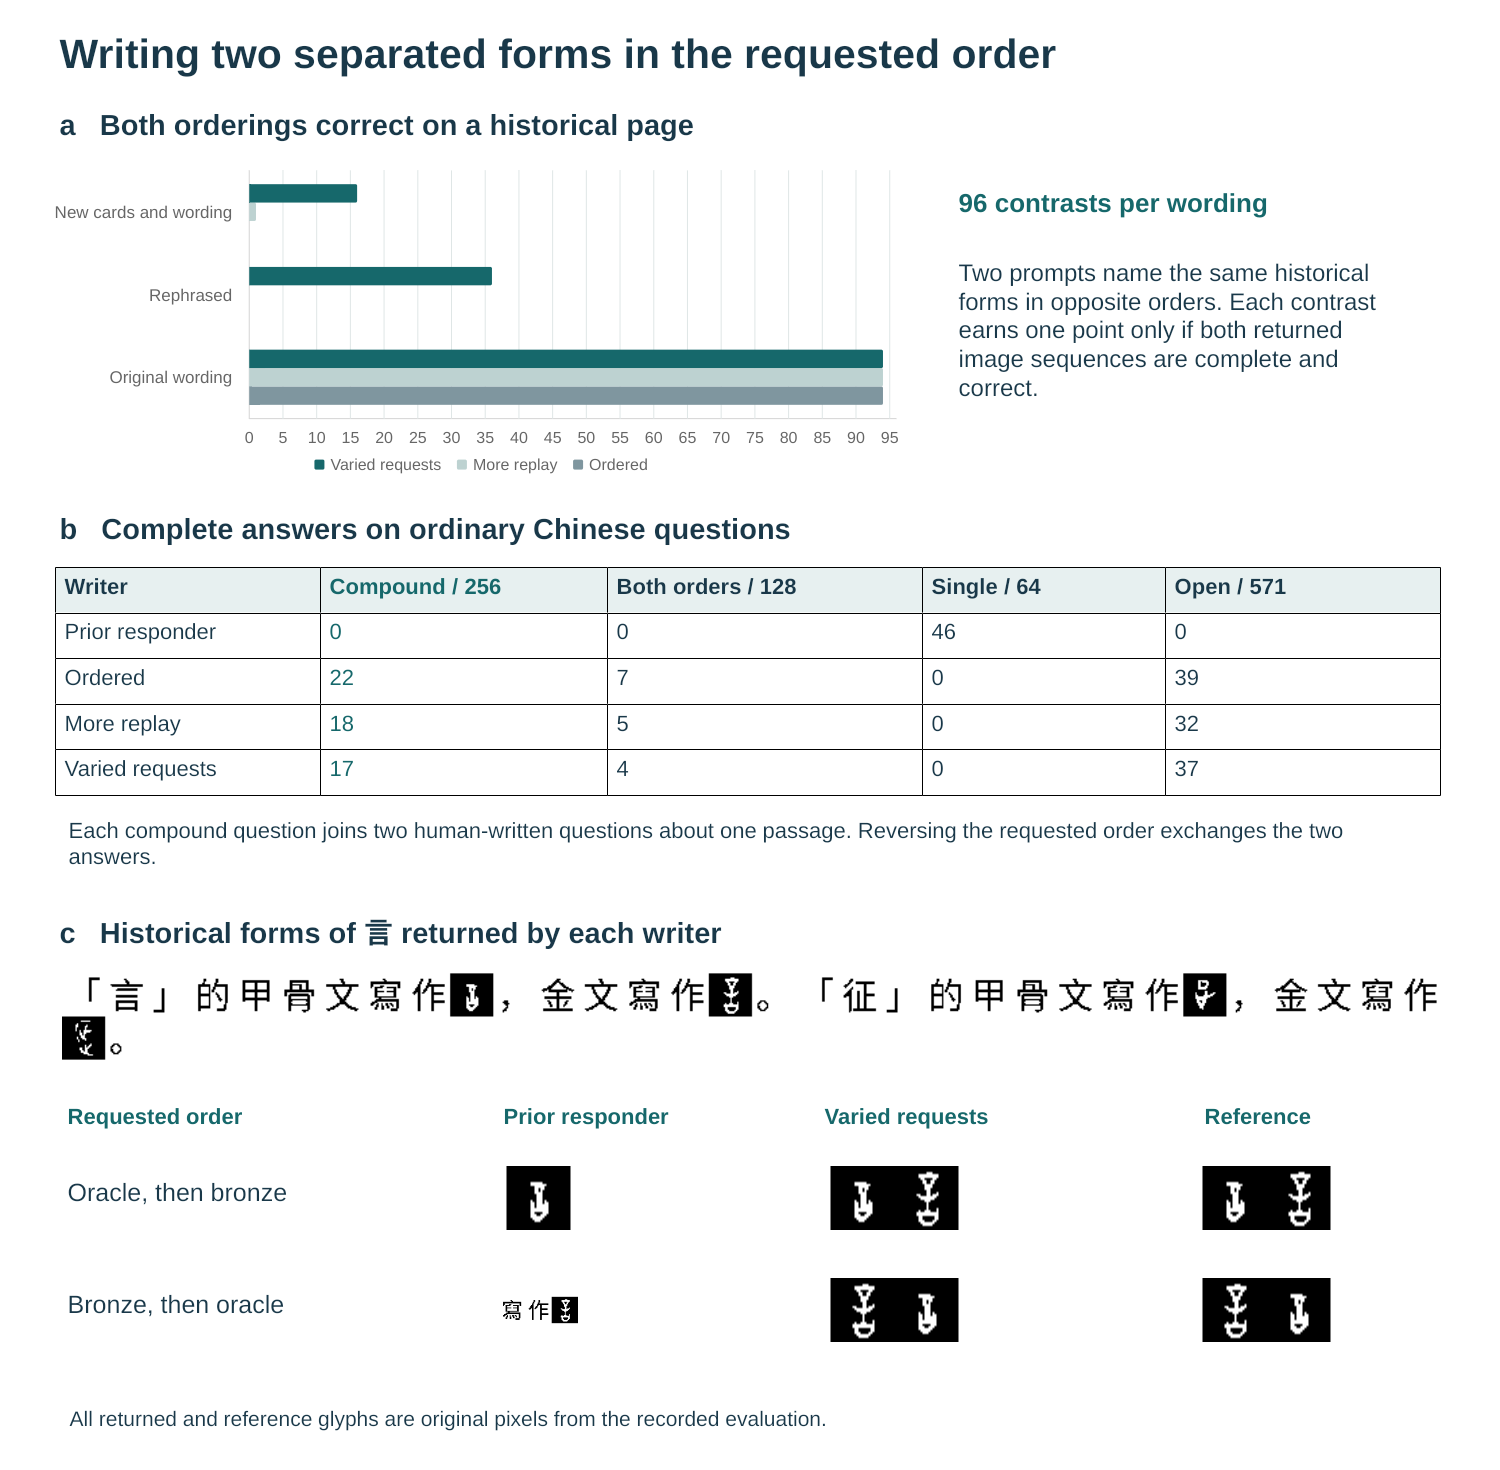
\includegraphics[width=.84\textwidth]{figures/Figure_89_ordered_page_writer.png}
\caption{\DIFaddFL{\textbf{Ordered writing across separated source images.}
\textbf{a}, Complete reversals on held-out historical pages. Two prompts ask for the same two forms in opposite orders. Each condition has 96 paired comparisons. The third uses 24 further cards and phrasing fixed before the request-variation fit. Replay and varied requests start from the same ordered writer and receive the same number of updates.
\textbf{b}, Exact stopped answer images on natural paired CMRC questions, the 64 individual role questions, and 571 open DuReader cases. The both-orders column counts CMRC pairs for which both complete answers are correct.
\textbf{c}, The same two-entry plate supplies the source for opposite requests about \textit{yan} (U+8A00). Columns show the returned pixels and the two source forms in the requested order. The depicted card belongs to the historical training-family partition.}}
\label{fig:ordered-page-writer}
\end{figure*}
\begin{figure*}[p]
\centering
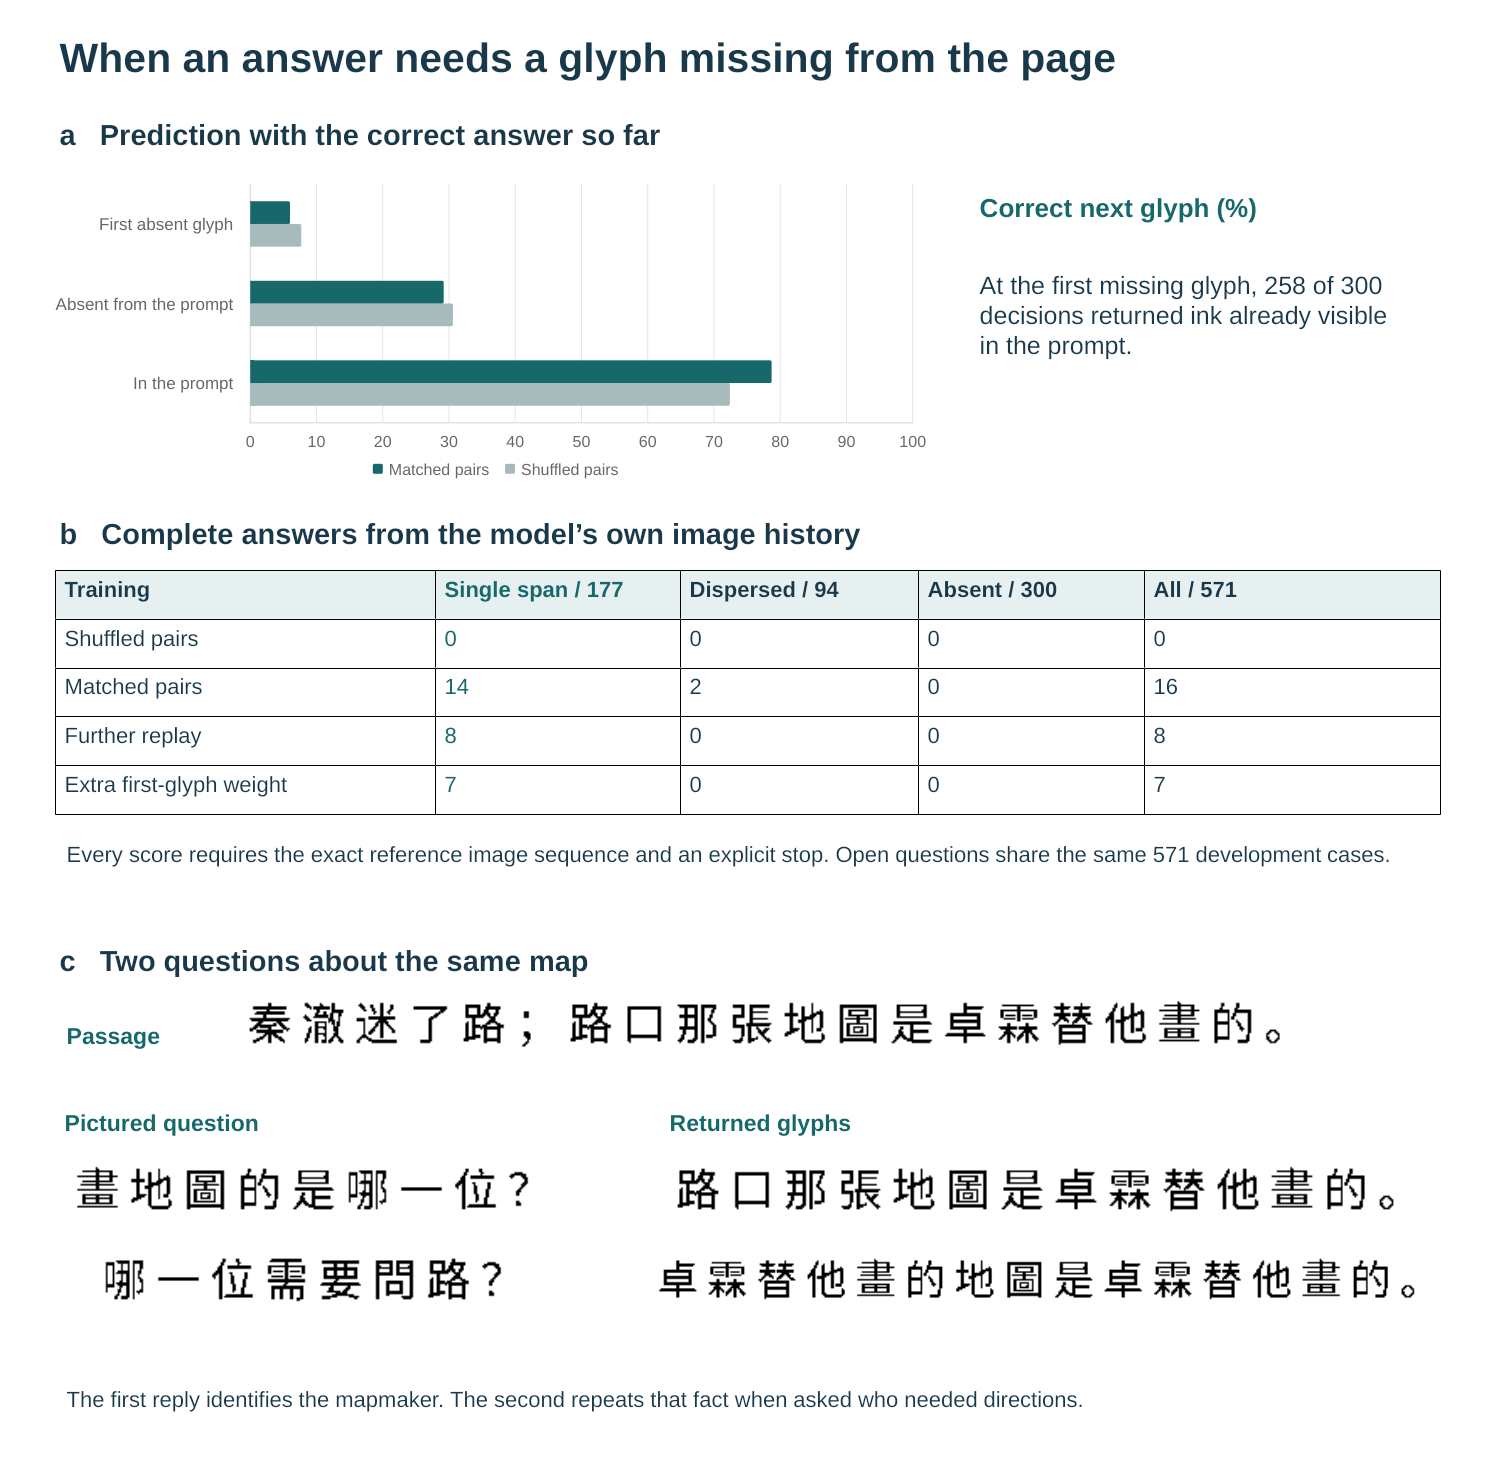
\includegraphics[width=.84\textwidth]{figures/Figure_90_causal_glyph_writer.png}
\caption{\DIFaddFL{\textbf{The first glyph absent from a pictured prompt.}
\textbf{a}, Next-glyph accuracy with the correct preceding answer. The groups comprise 12,764 target positions whose glyph is on the page, 1,525 whose glyph is absent and the first absent position in each of 300 cases. End decisions are excluded. The two training conditions use the same target batches.
\textbf{b}, Exact, explicitly stopped answer images on the 571 development questions. Further replay and extra weight on the first absent glyph start from the same matched checkpoint.
\textbf{c}, Original input and output pixels for the first two fixed role questions. Qin Che loses the way and Zhuo Lin draws the map. Asked who drew it, the model replies that Zhuo Lin drew it for him. Asked who needed directions, it repeats the mapmaking fact.}}
\label{fig:causal-glyph-writer}
\end{figure*}
\begin{figure*}[p]
\centering
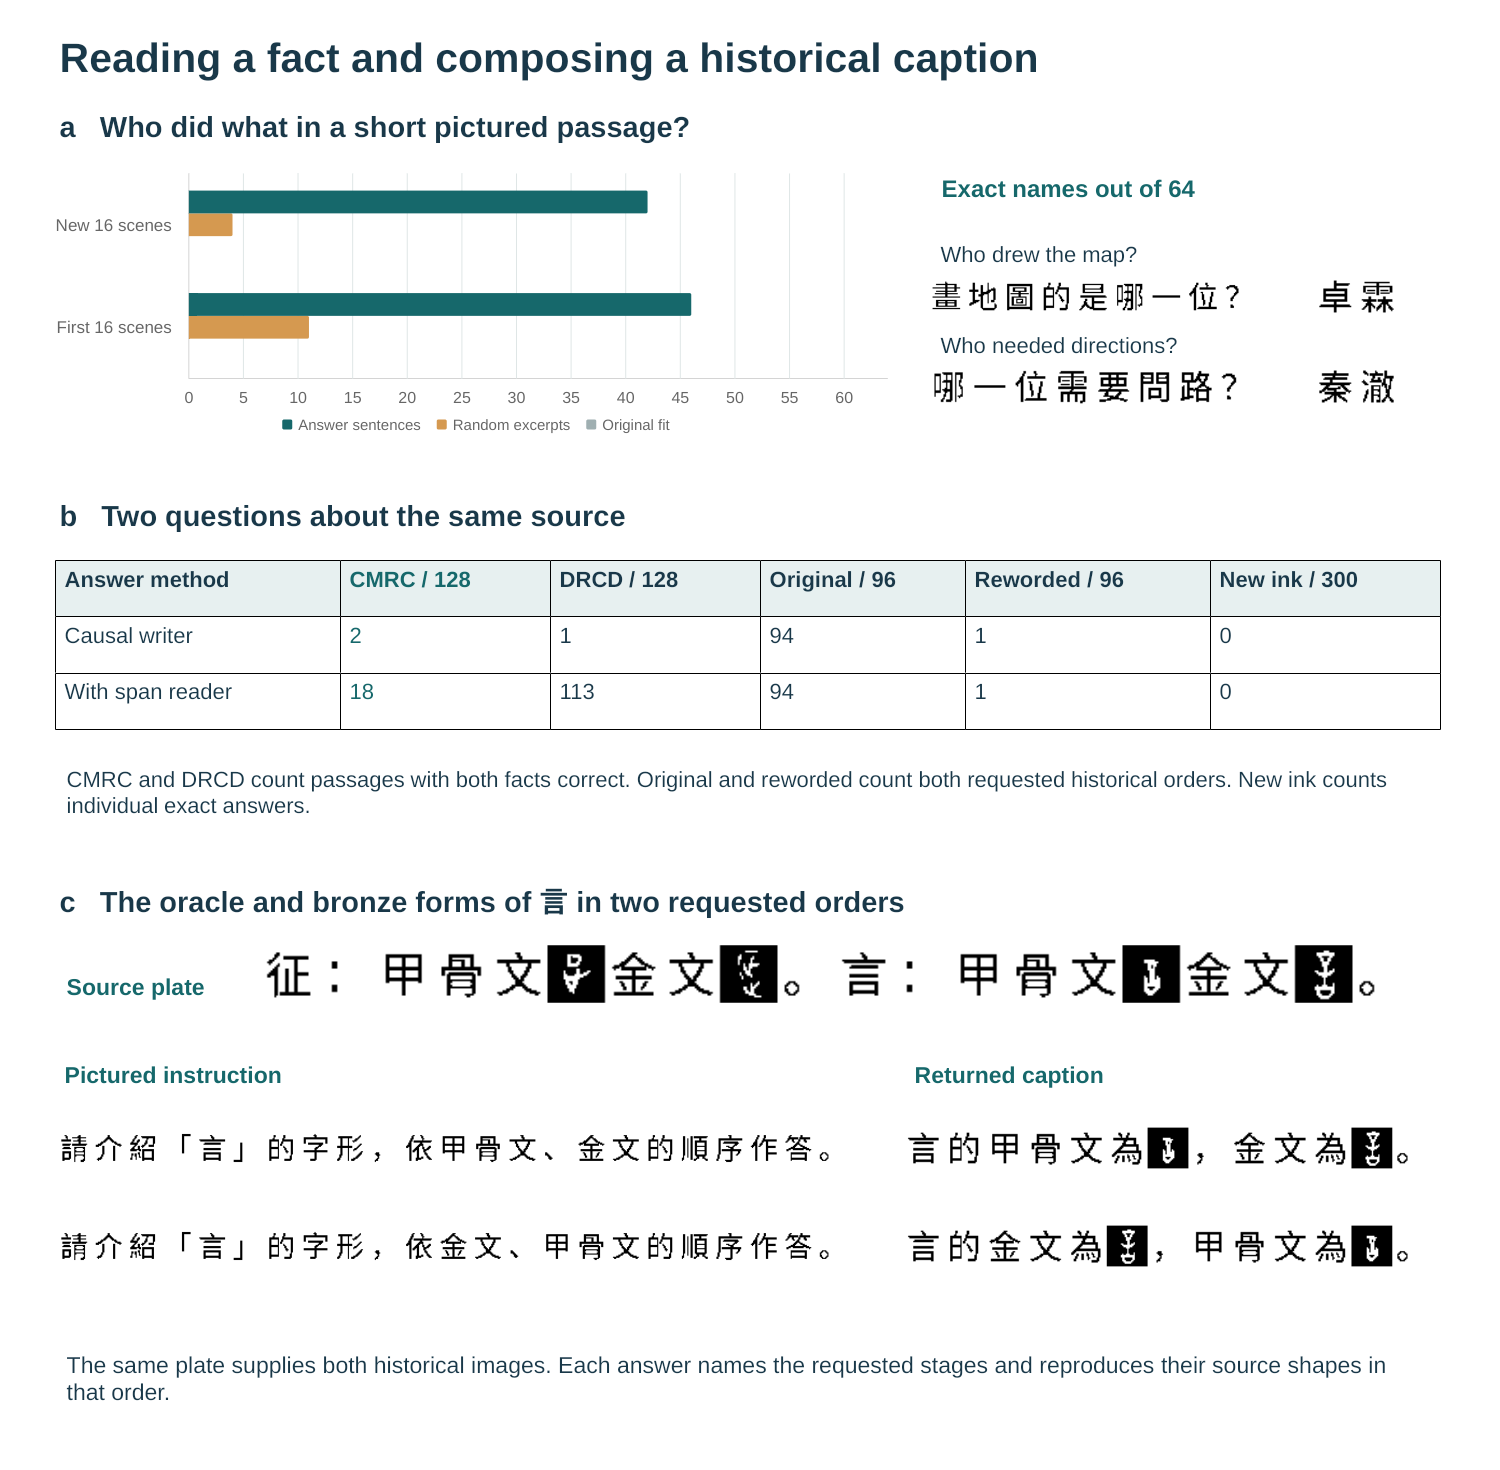
\includegraphics[width=.84\textwidth]{figures/Figure_91_pointing_causal_writer.png}
\caption{\DIFaddFL{\textbf{Quoting a fact and composing an answer with historical glyphs.}
\textbf{a}, Exact participant names across two questions and two assignments of names for each of sixteen situations in each cohort. Original pictured questions and returned answers show the mapmaker (Zhuo Lin) and the person needing directions (Qin Che). The short-sentence fit quotes the correct name in each case.
\textbf{b}, Both questions must receive exact answers for each natural passage. In the two historical columns, both complete captions for one headword must contain the requested source bitmaps in the correct order. The last column counts individual answers requiring a content glyph absent from the pictured prompt.
\textbf{c}, The specified demonstration plate for \textit{yán} (speech) contains images of two families' historical forms. Its two requests ask for oracle and bronze, first in chronological order and then in reverse. Each original answer strip interleaves copied forms with printed connecting text. This card comes from a training family and is separate from the 96 held-out comparisons.}}
\label{fig:pointing-causal-writer}
\end{figure*}
\begin{figure*}[p]
\centering

\includegraphics[width=.84\textwidth]{figures/Figure_92_grounded_proposition.png}
\caption{\DIFaddFL{\textbf{Two factual relations in a pictured answer.}
\textbf{a}, Complete two-sentence answers by training condition. Each passage is evaluated in both request orders with original and exchanged names. The denominators are 312 replies on practised combinations and 136 on withheld combinations.
\textbf{b}, Complete accepted statements on independently phrased questions and exact reference replies on the open set. Unlisted paraphrases can be valid.
\textbf{c}, Original output pixels for the first held-out passage, crediting the lyricist and singer in two assignments.
\textbf{d}, Original input and output pixels for the first independently written film note. The same person is credited twice, and the exchanged answer includes an extra character in the name.}}
\label{fig:grounded-proposition}
\end{figure*}
\begin{figure*}[p]
\centering
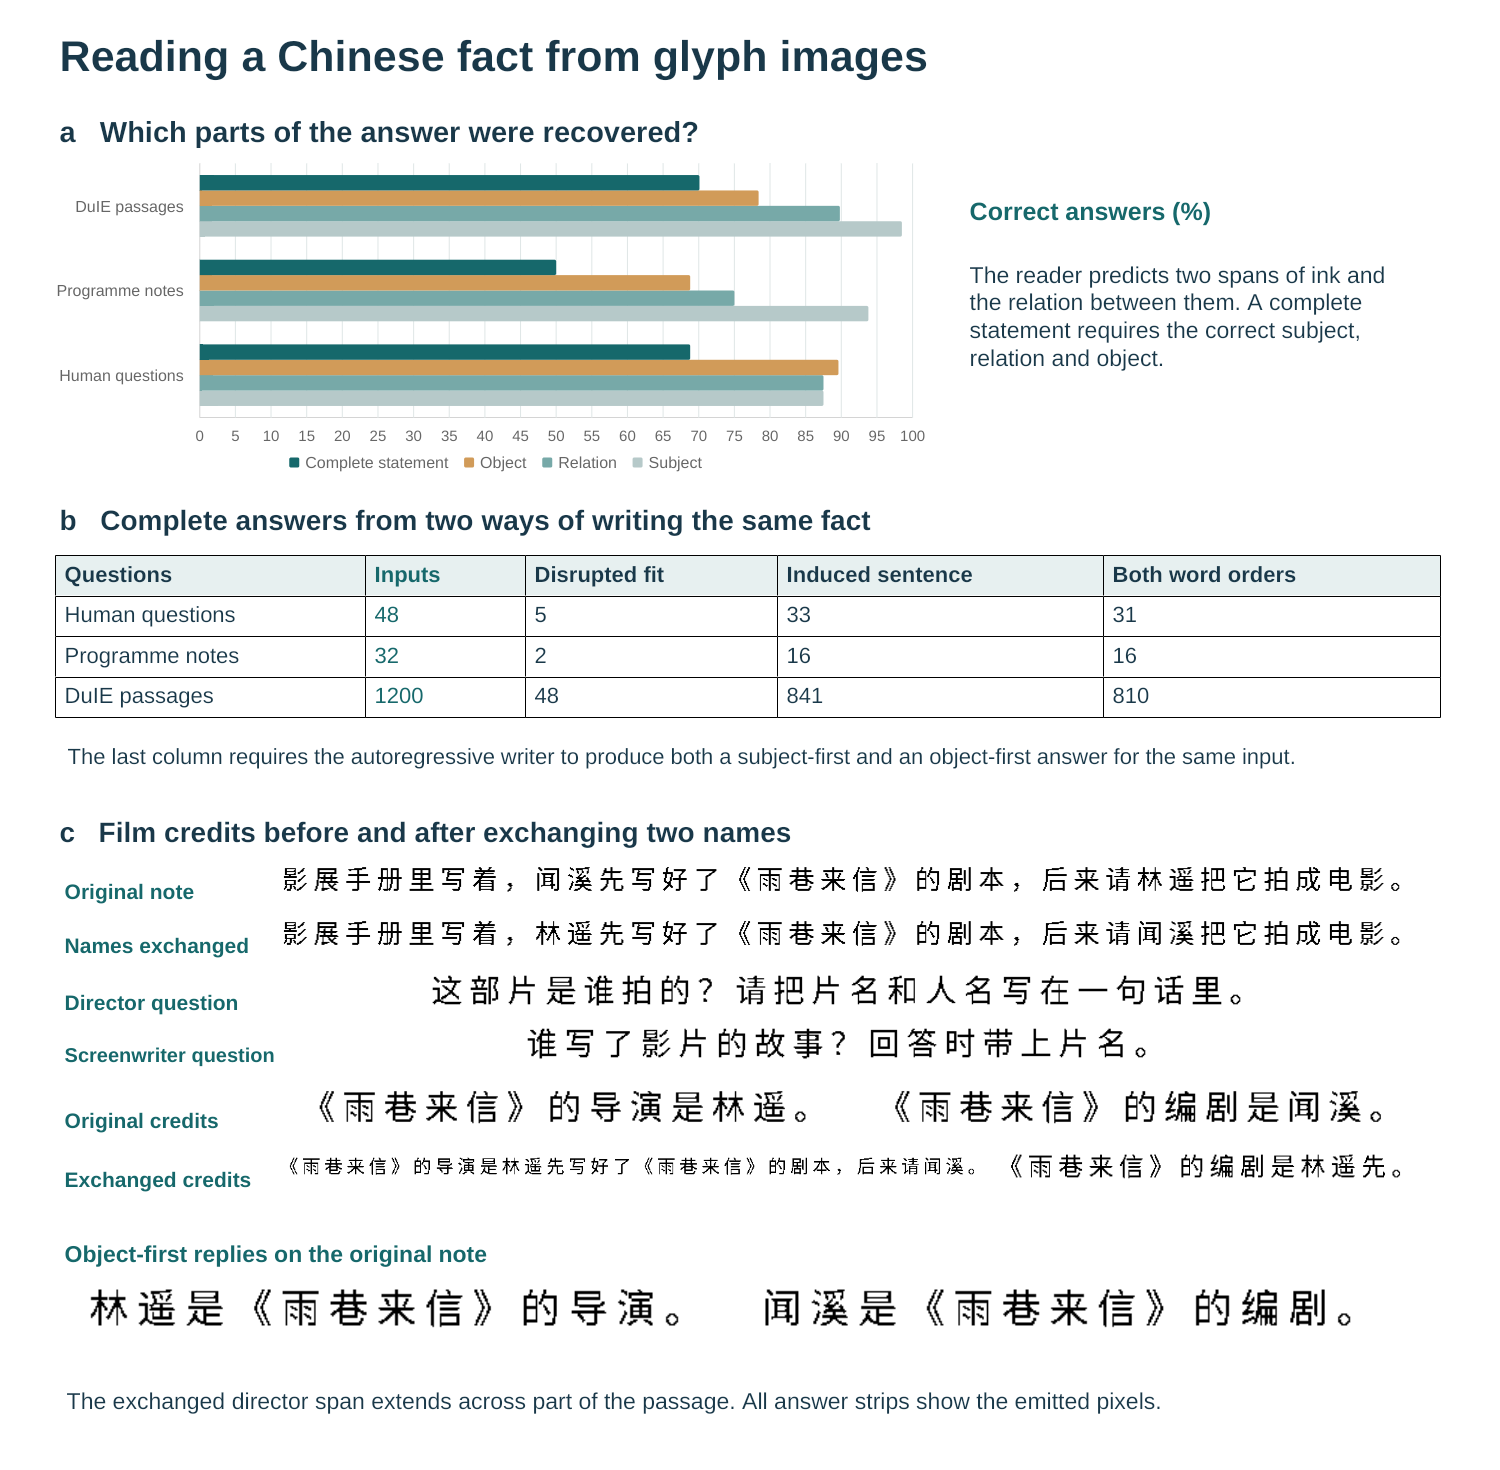
\includegraphics[width=.84\textwidth]{figures/Figure_93_role_binding.png}
\caption{\DIFaddFL{\textbf{Recovering the participants of a pictured fact and expressing it in two orders.}
\textbf{a}, Correct subjects, relations, objects and complete statements on 48 human questions, 32 programme questions and 1,200 held-out DuIE passages. Each component is scored across the entire cohort.
\textbf{b}, Counts of complete replies with disrupted field supervision and with the induced writer. The last column requires two stopped, exact answers to the same question from the autoregressive writer, first leading with the subject and then with the object.
\textbf{c}, Original film notes, questions and emitted strips. Credits run from director at left to screenwriter at right. On the exchanged source the first predicted name extends into a second clause. At bottom, the autoregressive writer starts both original credits with the correct person.}}
\label{fig:role-binding}
\end{figure*}
\begin{figure*}[p]
\centering
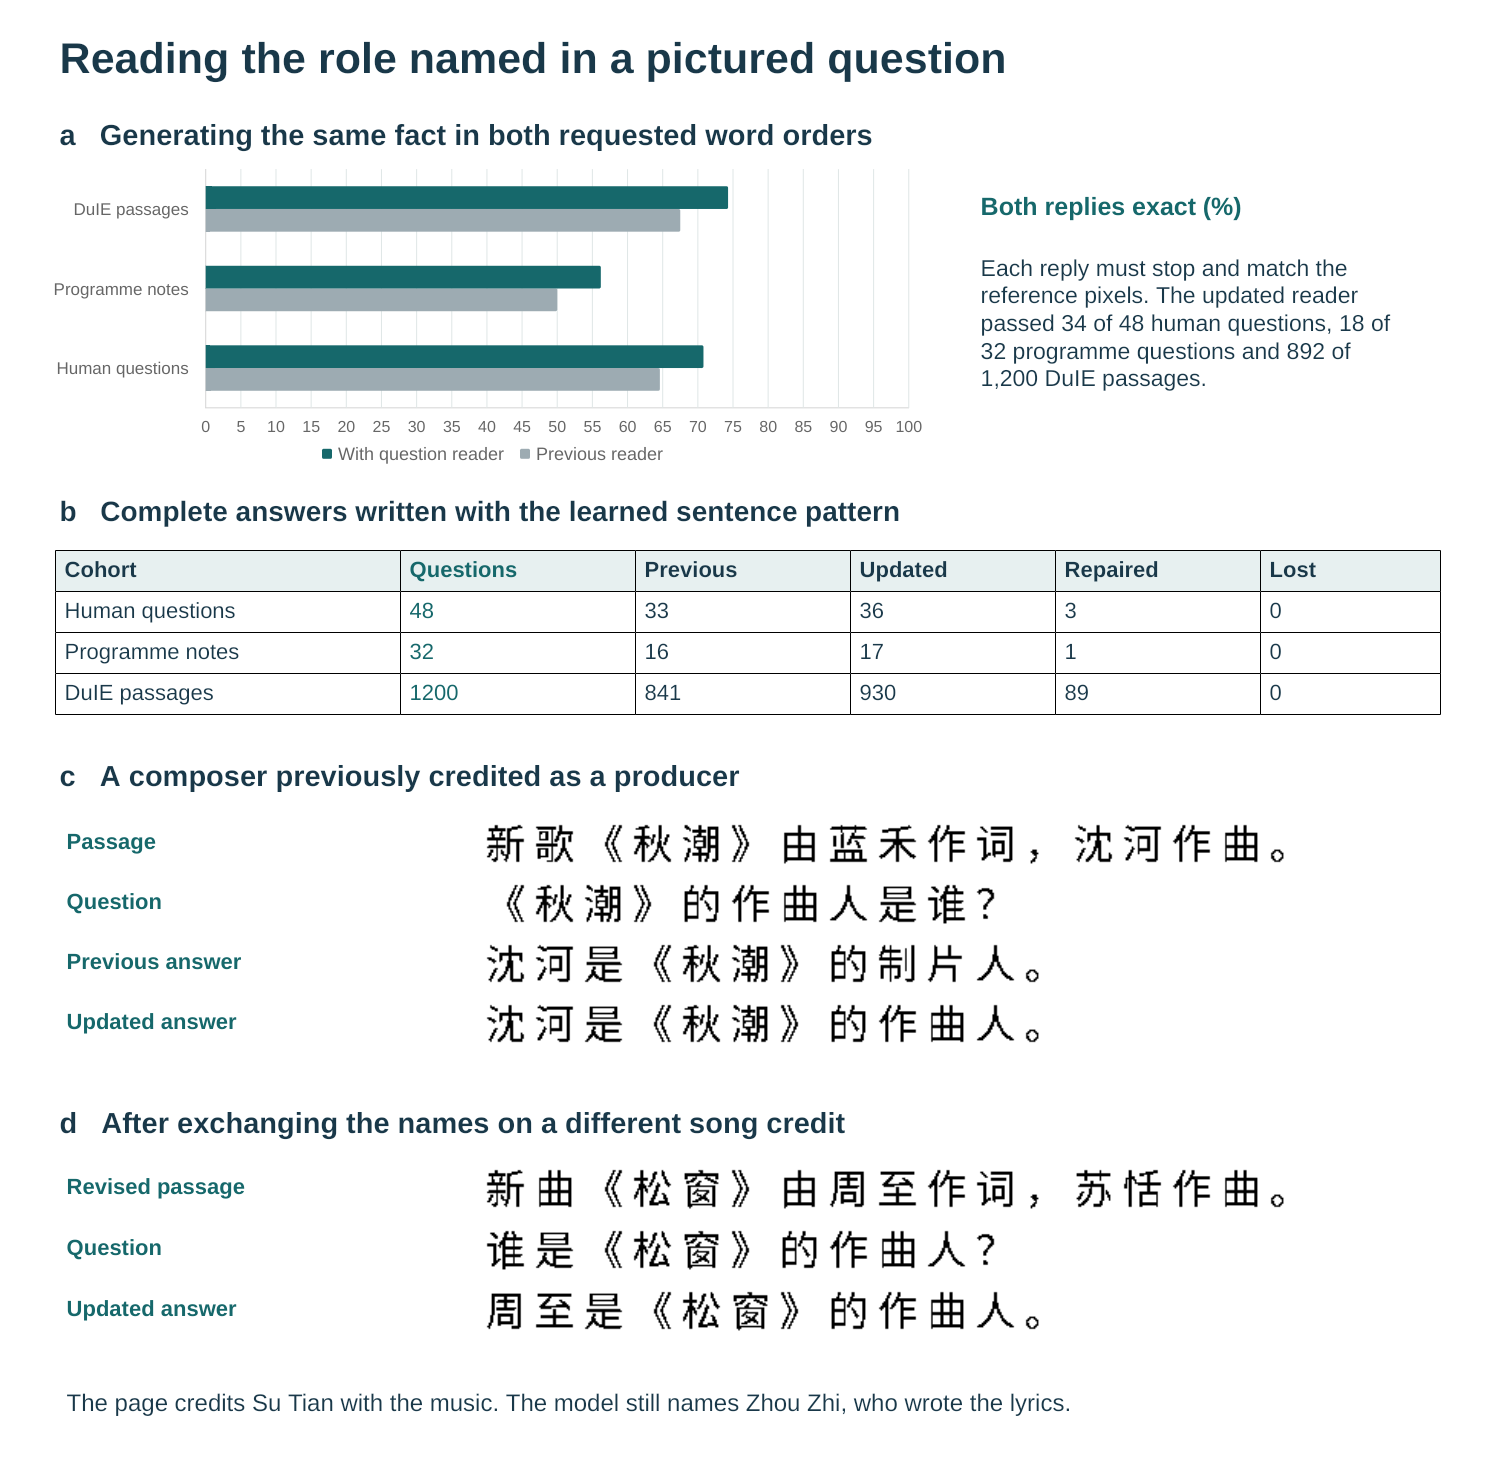
\includegraphics[width=.84\textwidth]{figures/Figure_94_pictured_relation.png}
\caption{\DIFaddFL{\textbf{Reading the requested role and copying the correct person.}
\textbf{a}, Percentage of questions with stopped, pixel-exact answers in both requested word orders. Both readers use the same autoregressive writer.
\textbf{b}, Exact statements with the learned sentence pattern. Repairs and losses compare the same inputs before and after adding the question reader.
\textbf{c}, The original diagnostic and actual object-first replies. Both name Shen He. The updated output identifies him as the composer.
\textbf{d}, In a separate song with exchanged names, the model identifies the role but copies the lyricist instead of the composer. All displayed Chinese strips are original input or emitted pixels.}}
\label{fig:pictured-relation}
\end{figure*}
\begin{figure*}[p]
\centering
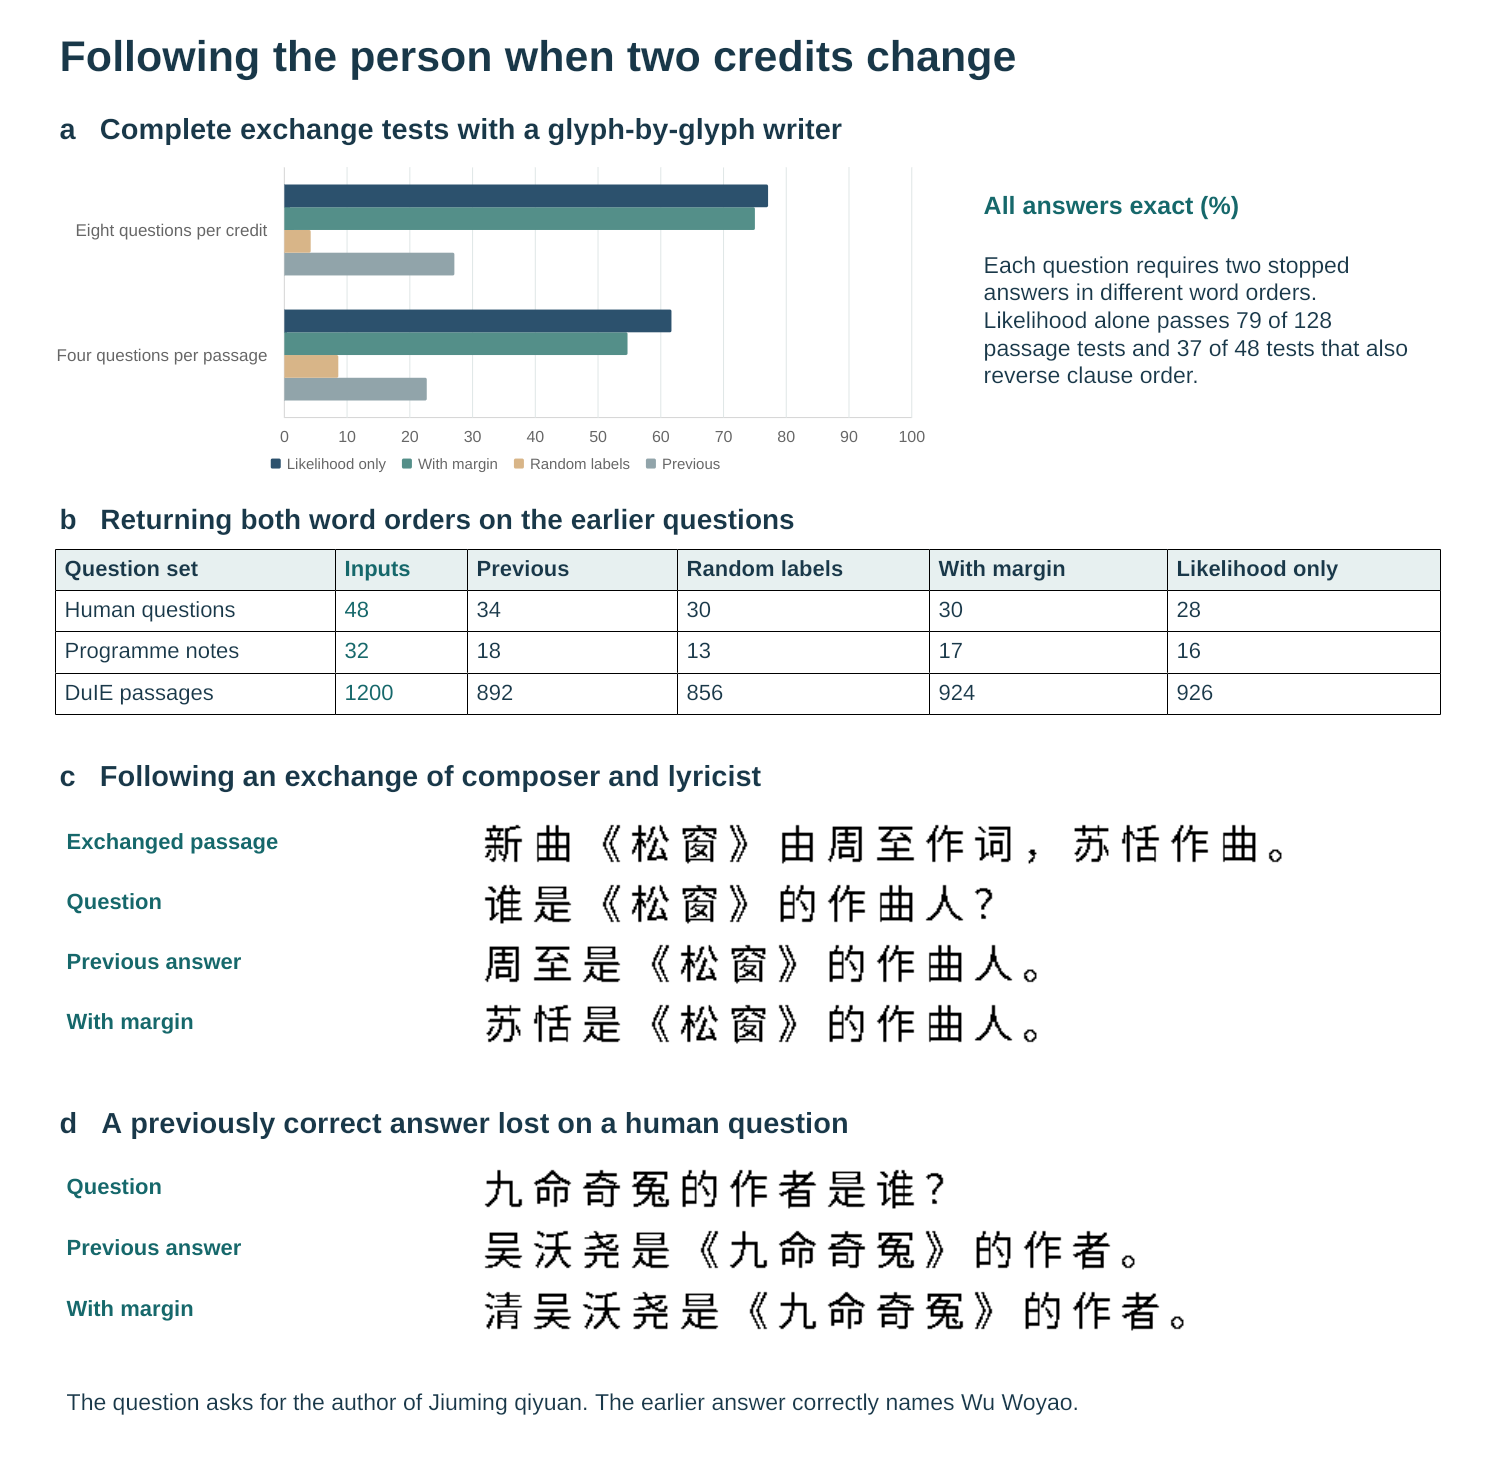
\includegraphics[width=.84\textwidth]{figures/Figure_95_participant_margin.png}
\caption{\DIFaddFL{\textbf{A visual reader follows exchanged credits while losing accuracy on broader questions.}
\textbf{a}, Fraction of passages passing every requested word order, role and name assignment. The clause-order test also reverses the order of the two clauses.
\textbf{b}, Counts of questions with two stopped, pixel-exact replies from the same autoregressive writer. The likelihood-only fit used the same correct labels and omitted the extra margin penalty.
\textbf{c}, Original input and output pixels from the song that exposed the error in Figure~\ref{fig:pictured-relation}. The revised answer names Su Tian.
\textbf{d}, First human question in evaluation order on which the earlier writer passed both orders and the new scorer lost one. Both name Wu Woyao. The new object-first reply also copies the character identifying the Qing dynasty.}}
\label{fig:participant-margin}
\end{figure*}
\begin{figure*}[p]
\centering
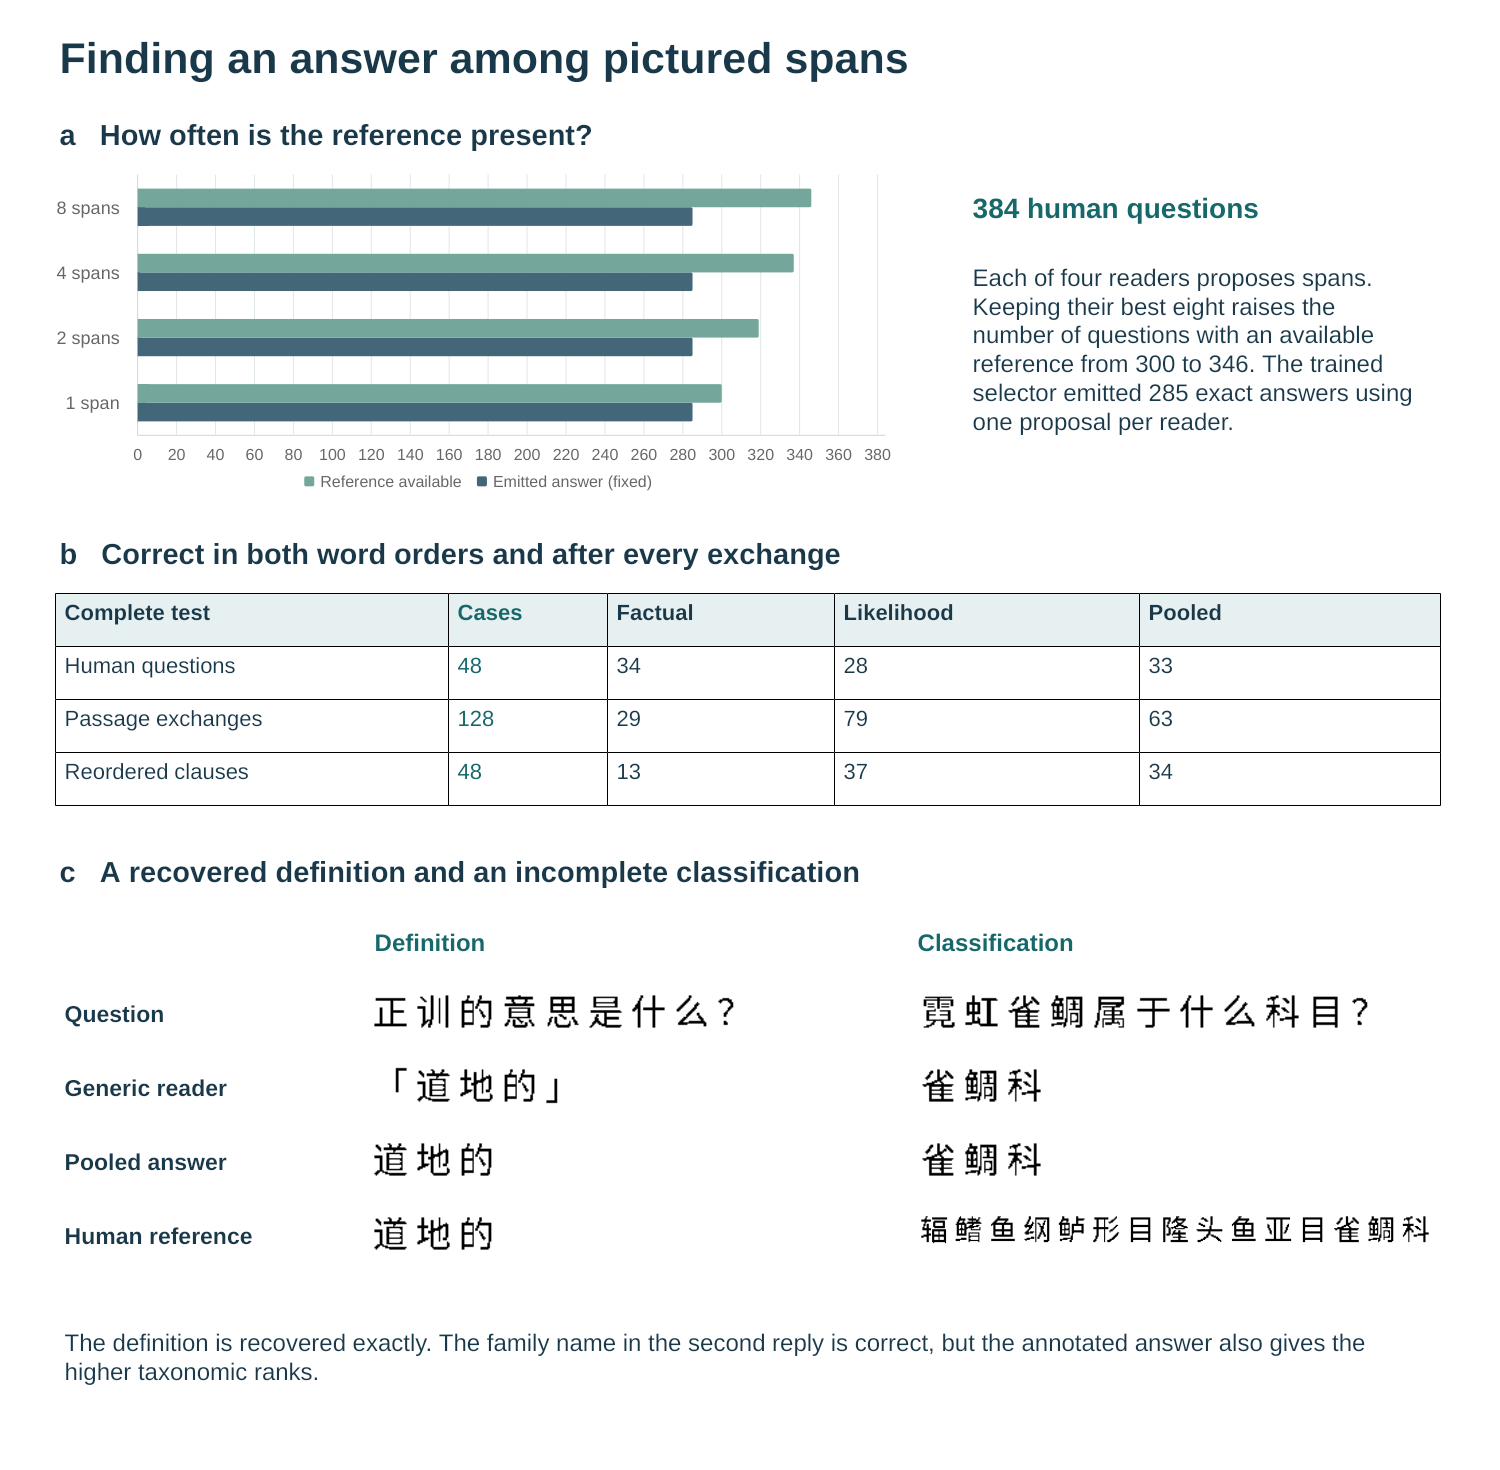
\includegraphics[width=.84\textwidth]{figures/Figure_96_span_choice.png}
\caption{\DIFaddFL{\textbf{Availability of a correct pictured answer limits learned selection.}
\textbf{a}, Counts among 384 human questions. The fixed selector receives one span from each reader. The second series counts any matching reference as the span lists widen. Additional proposals were scored only for coverage.
\textbf{b}, Cases with exact stopped replies in both requested word orders. Passage-exchange tests additionally require both roles before and after exchanging the two names; the reordered tests add both clause orders.
\textbf{c}, Original pixels from the first recovered generic error and the first missing reference in evaluation order. The definition is exact. The classification reply gives the damselfish family; the annotation also includes the class, order and suborder.}}
\label{fig:span-choice}
\end{figure*}
\begin{figure*}[p]
\centering
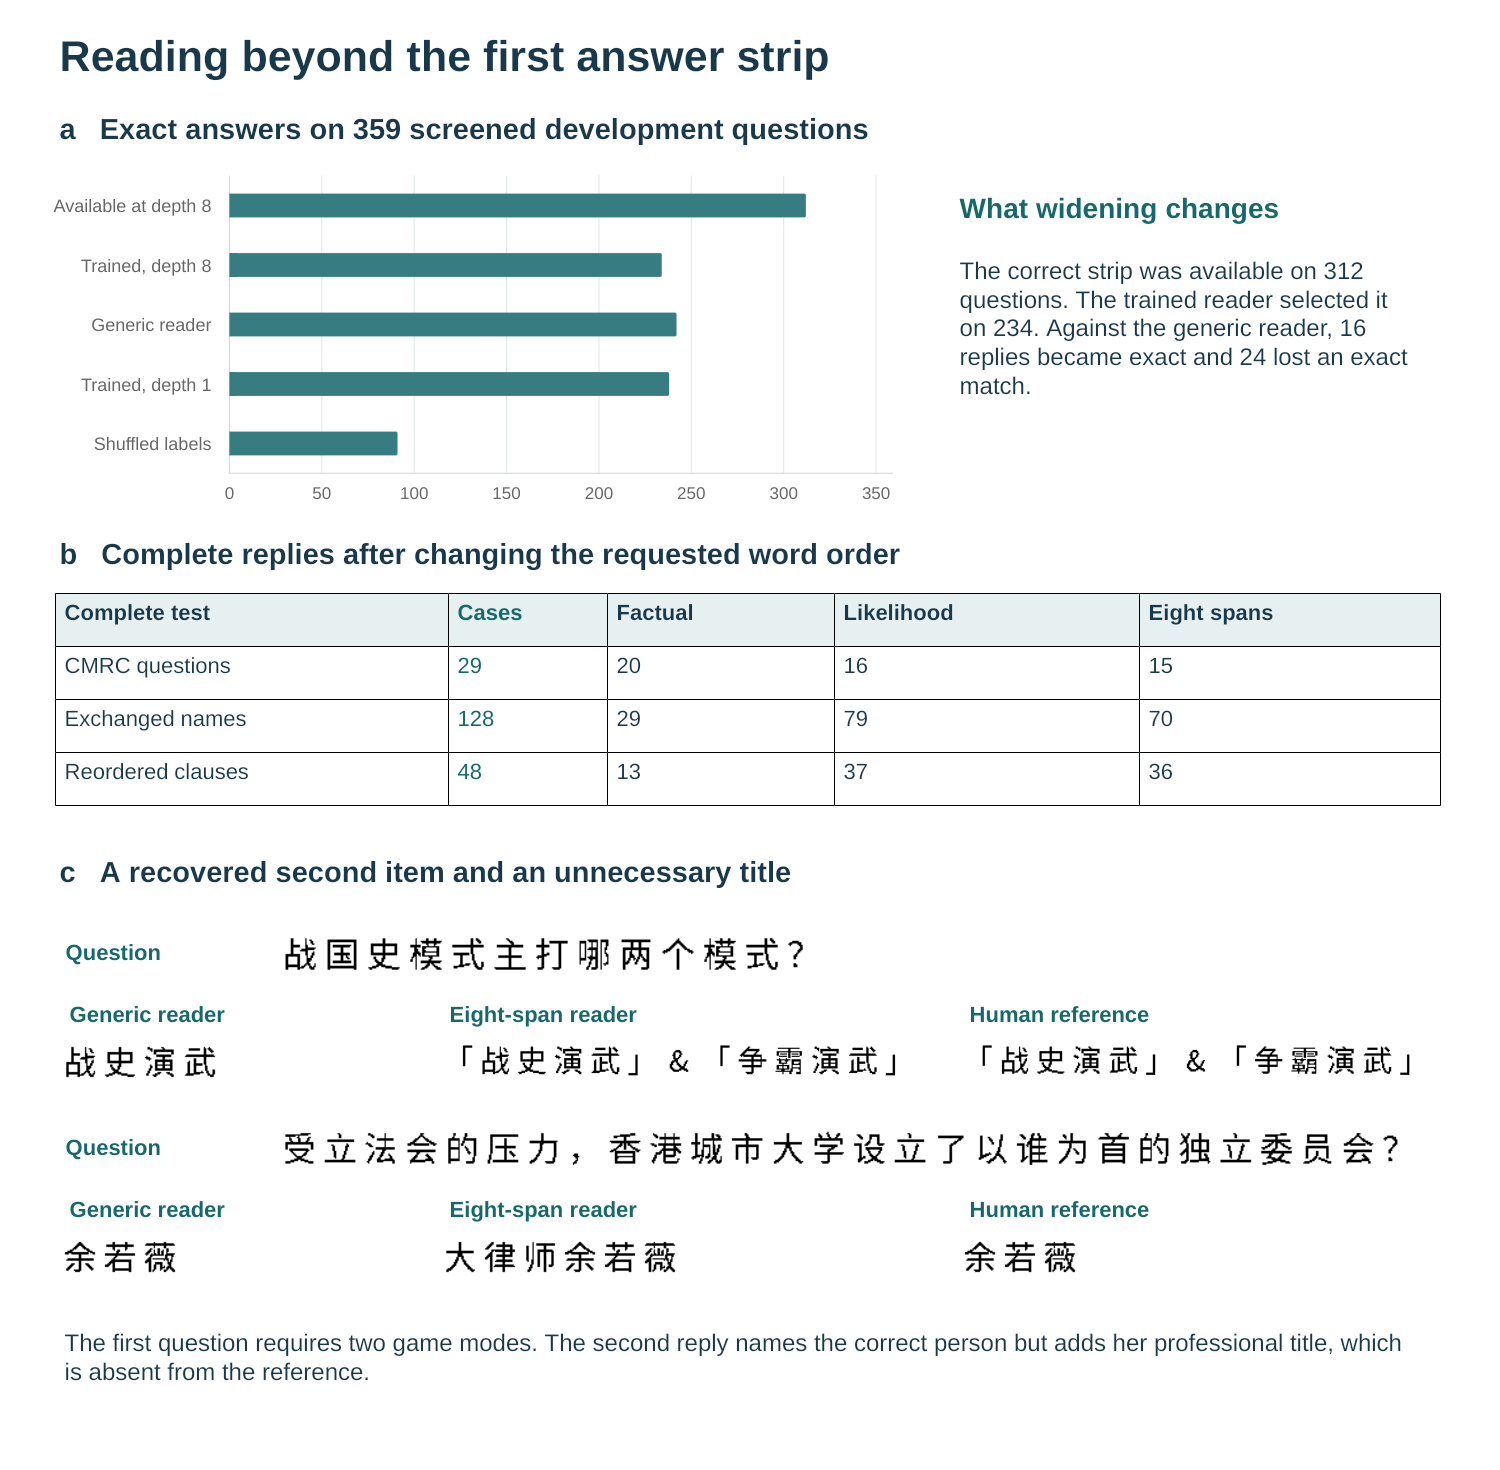
\includegraphics[width=.84\textwidth]{figures/Figure_97_span_list.png}
\caption{\DIFaddFL{\textbf{A wider list can contain the exact answer without improving selection.}
\textbf{a}, Exact reply counts on 359 screened development questions. The final bar counts questions for which an accepted reference was available at depth eight. It is an upper bound.
\textbf{b}, Cases on which every required stopped image reply in both word orders was exact. The last two rows also require both role assignments; the last additionally requires both clause orders.
\textbf{c}, Original question and answer images from the first recovered lower-ranked reference and first regression against the generic reader in fixed evaluation order. The recovered answer contains both requested game modes. The second answer includes a professional title before the correct name.}}
\label{fig:span-list}
\end{figure*}
\begin{figure*}[p]
\centering

\includegraphics[width=.84\textwidth]{figures/Figure_98_page_evidence.png}
\caption{\DIFaddFL{\textbf{Question wording changes whether a writer uses the year on a pictured page.}
\textbf{a}, New DuIE sources. A board counts once if every generated answer had the requested participant and year in a complete, exact sentence pair, with autonomous stopping under all three new question formulations.
\textbf{b}, The earlier evaluation pages. The fields-only control received the correct annotated participants and relation. Both ordinary word orders must pass for a DuIE or CMRC item. The clause row counts exact reproductions of source-authored text.
\textbf{c}, Original glyph strips from the varied-instruction writer. The top rows show the first complete single-page pair in fixed order. The lower rows show the first failed two-paragraph reply and its reference.}}
\label{fig:page-evidence}
\end{figure*}
\begin{figure*}[p]
\centering

\includegraphics[width=.84\textwidth]{figures/Figure_99_paragraph_evidence.png}
\caption{\DIFaddFL{\textbf{Finding evidence can correct a factual binding while leaving the writer unable to finish an answer.}
\textbf{a}, Complete comparisons with the same frozen writer. Each date comparison requires twelve correct terminated replies. Each quotation comparison requires four.
\textbf{b}, Correct evidence choices and remaining exact-answer errors on the annotated source. Human questions come from the simplified-script CMRC and traditional-script DRCD development sets.
\textbf{c}, Original emitted glyphs from the first corrected distinct-subject question and the first remaining error after correct selection. The omitted year is visible in the reference.}}
\label{fig:paragraph-evidence}
\end{figure*}
\begin{figure*}[p]
\centering
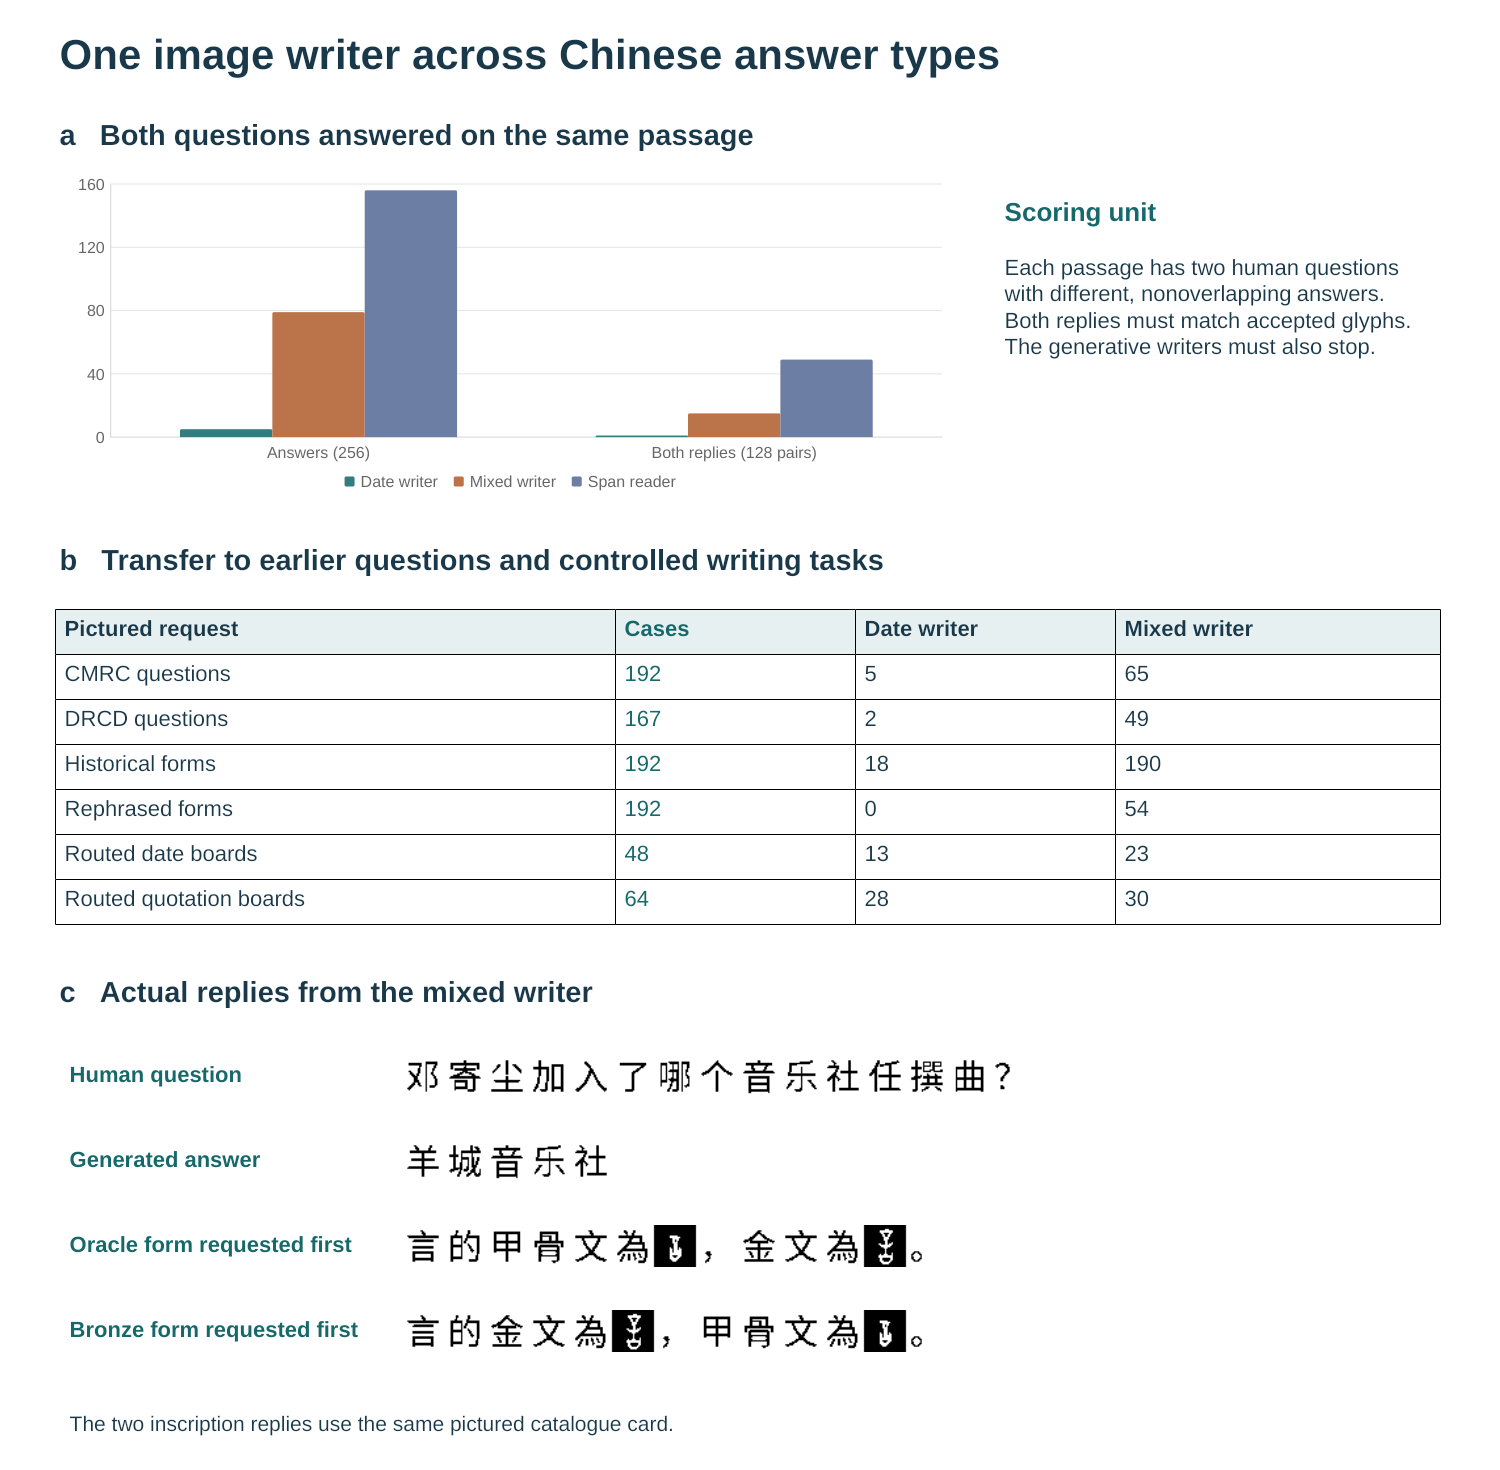
\includegraphics[width=.84\textwidth]{figures/Figure_100_mixed_visual_answers.png}
\caption{\DIFaddFL{\textbf{One set of writer weights reads natural questions and returns historical shapes in the requested order.}
\textbf{a}, Accepted answers across 256 new CMRC questions and passages with both answers accepted across 128 question switches. A frozen span reader selects an interval on the same page.
\textbf{b}, Earlier human questions and historical cards count individual exact, stopped replies. Date and quotation rows require every answer on the board. Both writers use the same learned paragraph selector in these two rows.
\textbf{c}, First exact mixed-writer reply in the additional CMRC comparison. The bottom strips are independently generated answers to the two orders of the known \textit{yan} catalogue card. All strips retain the recorded pixels.}}
\label{fig:mixed-visual-answers}
\end{figure*}
\begin{figure*}[p]
\centering
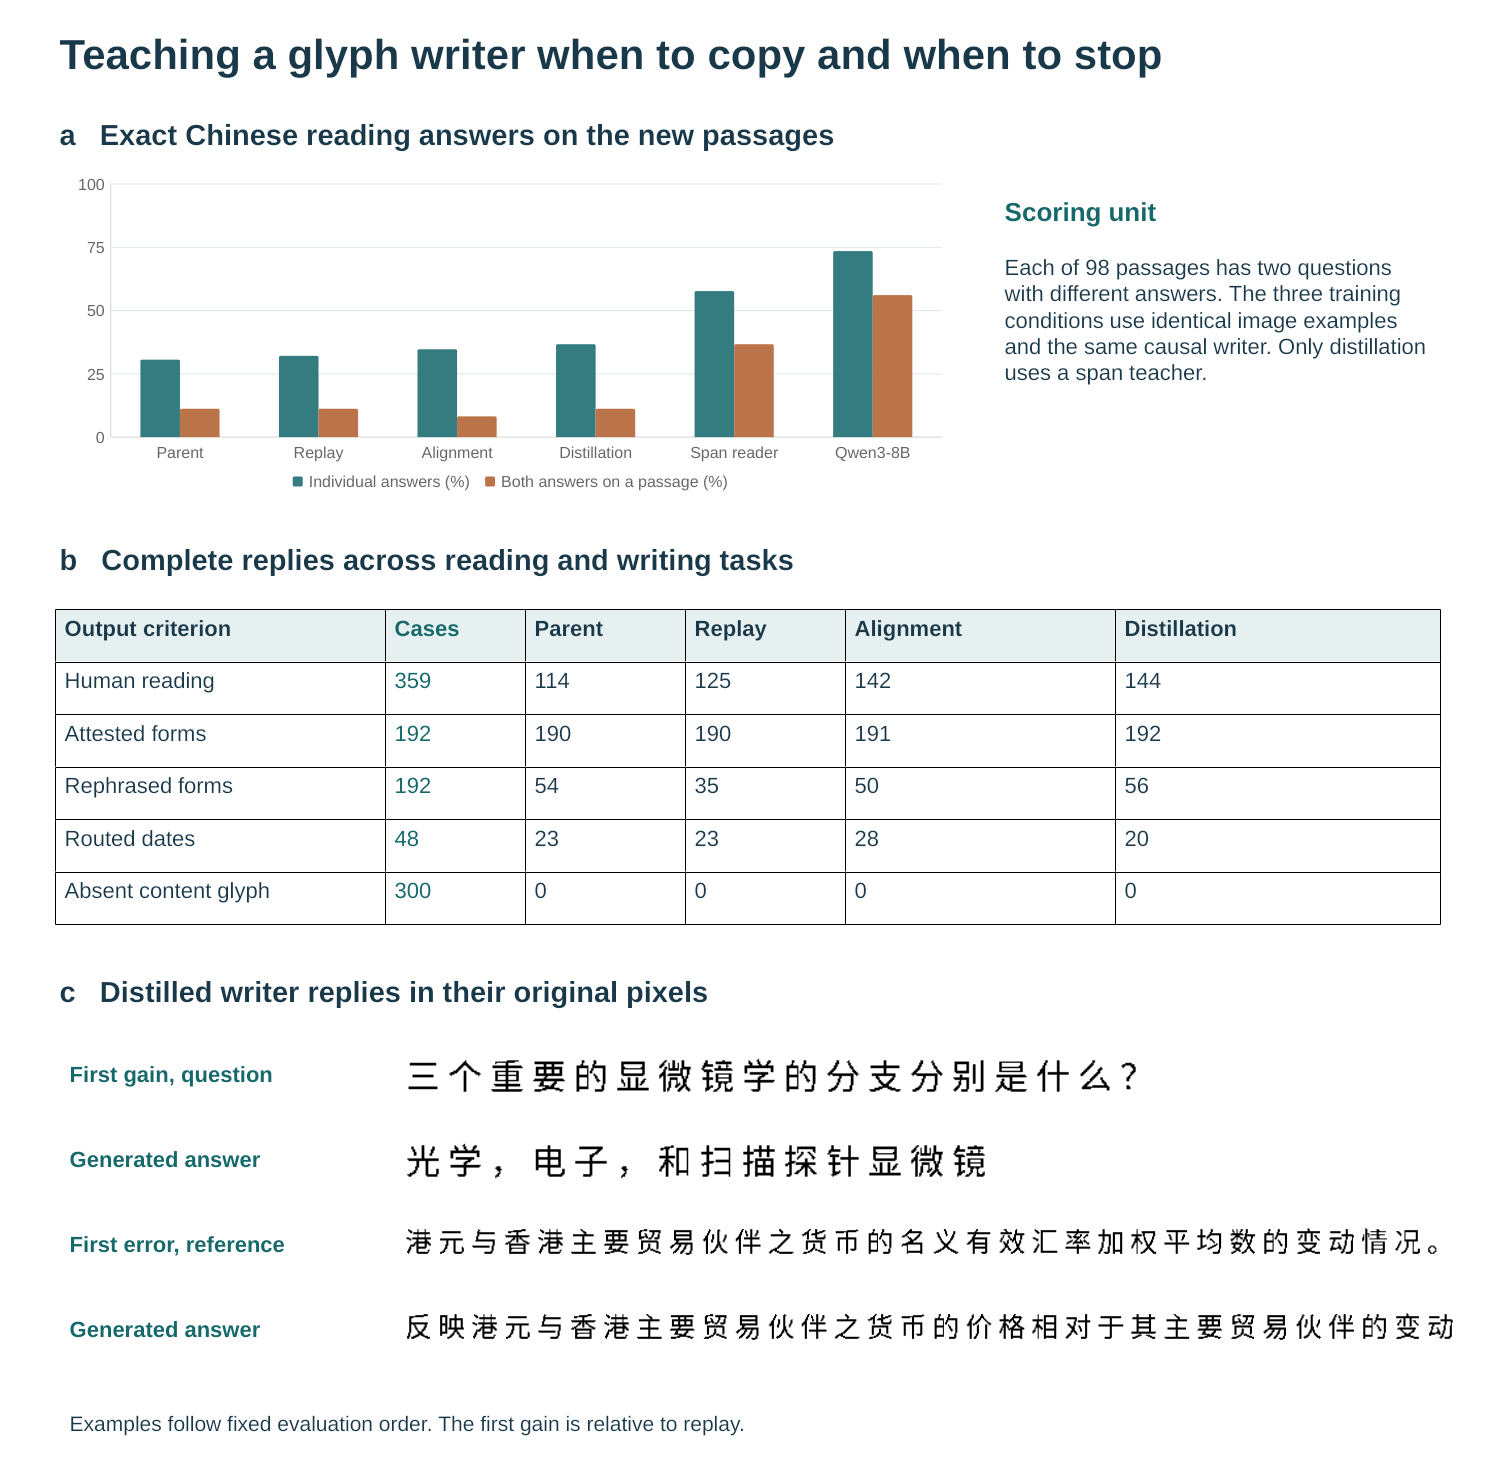
\includegraphics[width=.84\textwidth]{figures/Figure_101_interval_teacher.png}
\caption{\DIFaddFL{\textbf{Teaching a glyph writer to copy and stop on natural Chinese questions.}
\textbf{a}, Exact individual answers (196 questions) and passages with both distinct answers correct (98 passages). Qwen3-8B received the same material as text. The other models received glyph images.
\textbf{b}, Exact, stopped replies under four writer conditions. Routed dates require all twelve requests on a board to succeed. The last row counts exact canonical answers requiring at least one content glyph absent from the request and page.
\textbf{c}, Original question and answer strips for the first item gained by distillation over replay. Below them are the recorded reference and output for the first incorrect distilled reply. Examples follow fixed evaluation order.}}
\label{fig:interval-teacher}
\end{figure*}
\begin{figure*}[p]
\centering
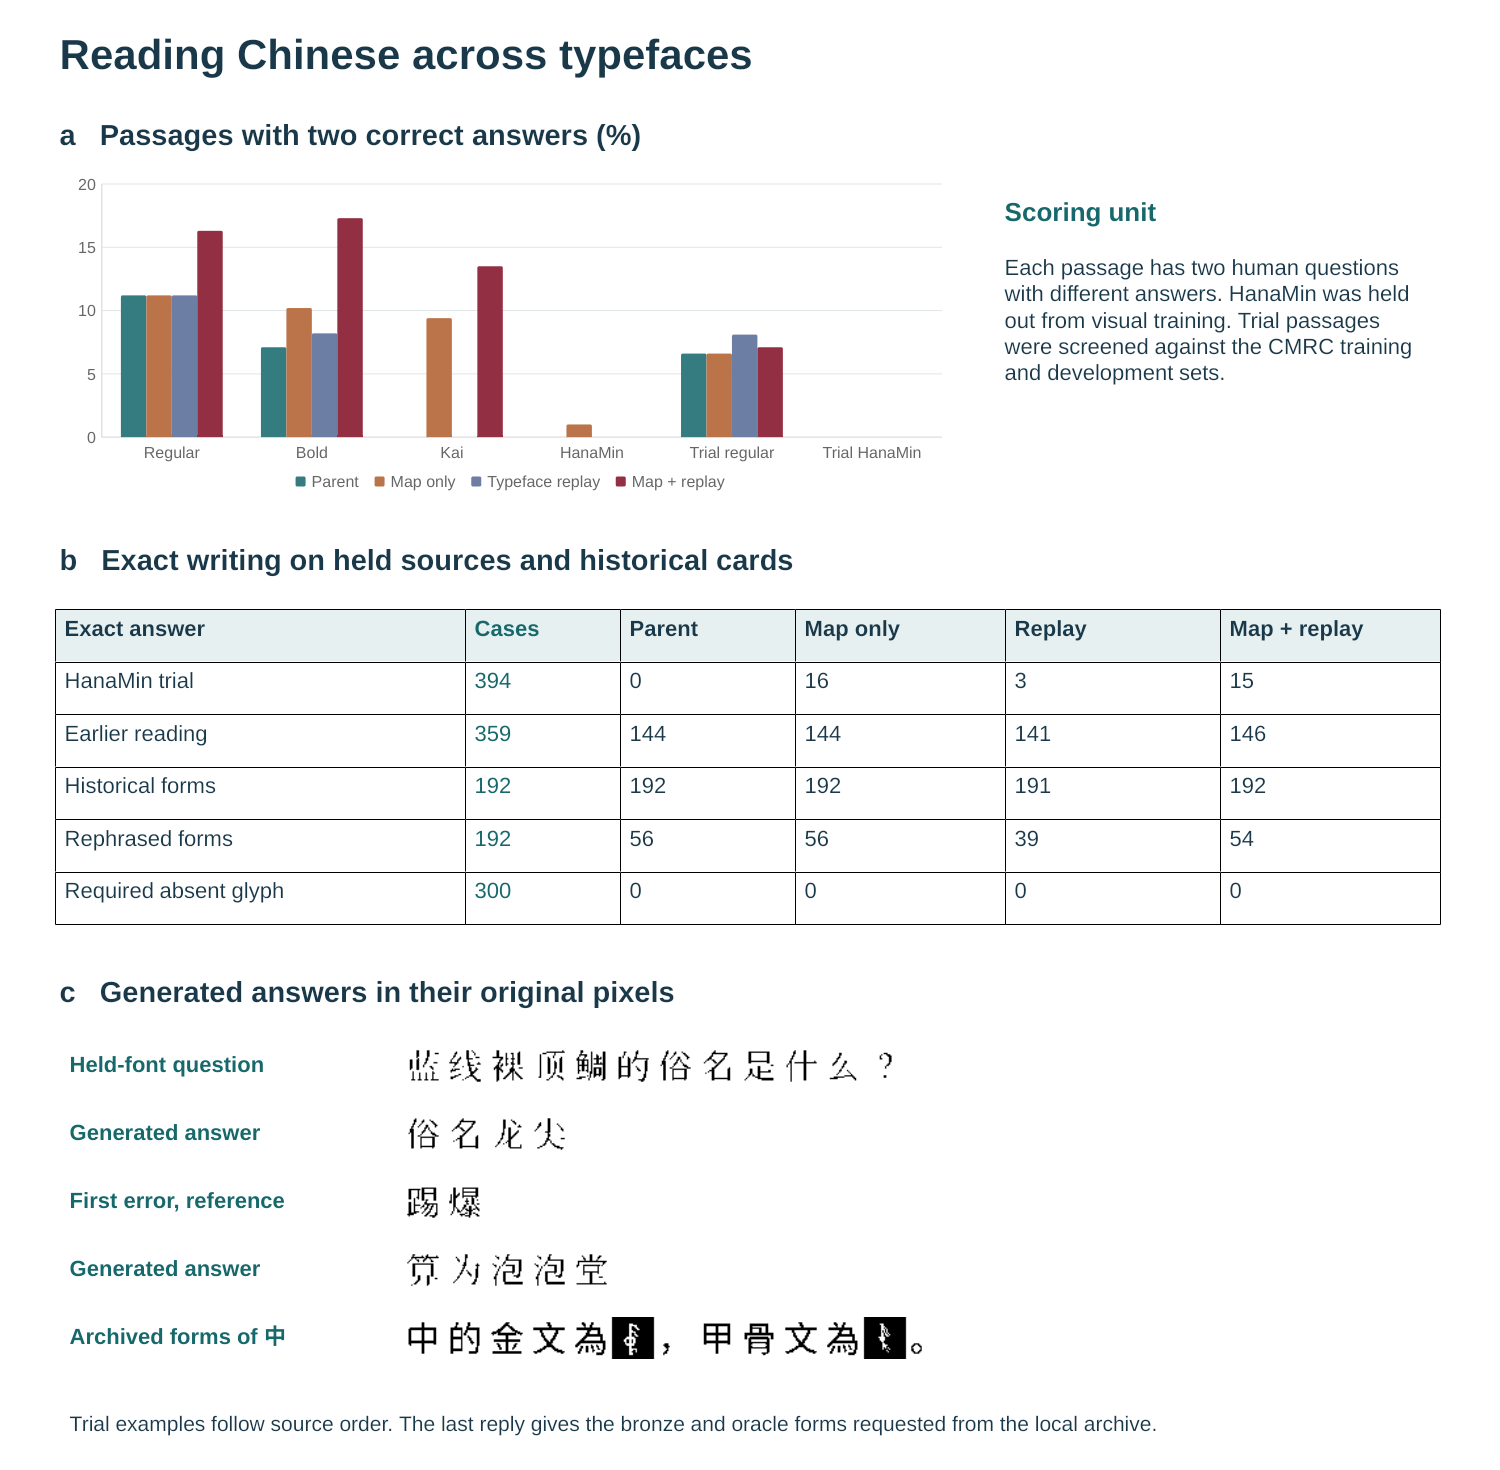
\includegraphics[width=.84\textwidth]{figures/Figure_102_typeface_writer.png}
\caption{\DIFaddFL{\textbf{Chinese reading after a change in typeface.}
\textbf{a}, Passages on which both distinct questions received a stopped, exact answer. The first four categories rerender the same 98 development passages, except for two passages excluded from Kai for missing glyphs. The final two categories use the renderable trial passages. Map only attaches the visual correspondence to the frozen parent. Both replay conditions receive the same additional printed examples.
\textbf{b}, Complete individual answers. Historical forms are copied from supplied evidence. The final row requires an answer containing a content glyph absent from the input.
\textbf{c}, Original pixels of a HanaMin trial question and generated reply, followed by the reference and output for the first error. The last strip is the offline writer's answer about the bronze and oracle forms of the headword \textit{zhong}. The catalogue records B00616 and J00887 for these two attestations.}}
\label{fig:typeface-writer}
\end{figure*}
\begin{figure*}[p]
\centering
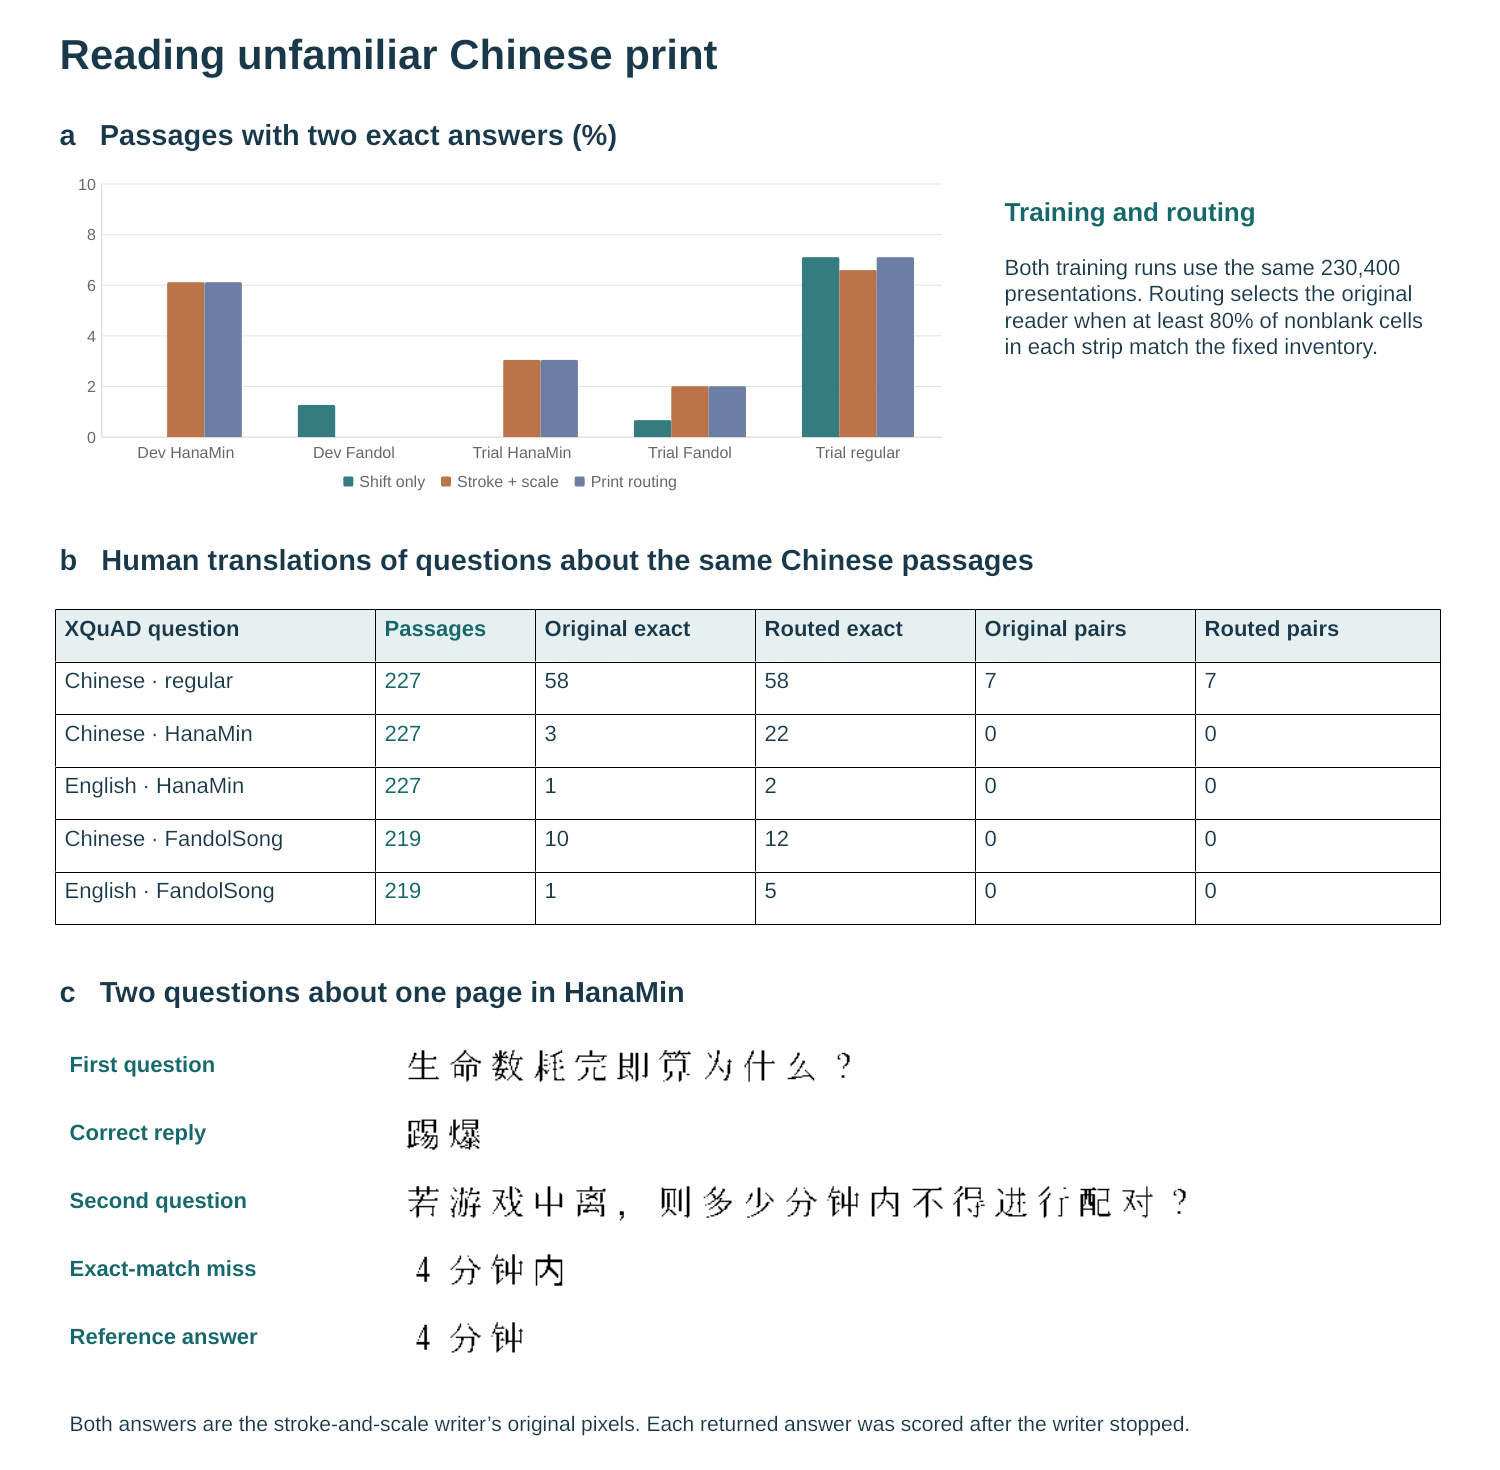
\includegraphics[width=.84\textwidth]{figures/Figure_103_stroke_scale.png}
\caption{\DIFaddFL{\textbf{Visual recognition and question answering after changes in stroke thickness and aspect ratio.}
\textbf{a,} Percentage of CMRC passages for which both questions receive an exact stopped answer. Each group compares a translation-only fit, a matched augmentation fit and the subsequent input-dependent print route. Fandol denotes FandolSong Regular. The language writer is shared. \textbf{b,} XQuAD paired questions about Chinese passages. Original and routed columns count complete answer images and passages with both questions correct. The denominator for individual answers is twice the number of passages. English questions request answers from the Chinese source. \textbf{c,} Original generated pixels for the first two CMRC trial questions in HanaMin. The second reply includes the reference duration and adds a glyph, causing an exact-match error.}}
\label{fig:stroke-scale}
\end{figure*}
\begin{figure*}[p]
\centering
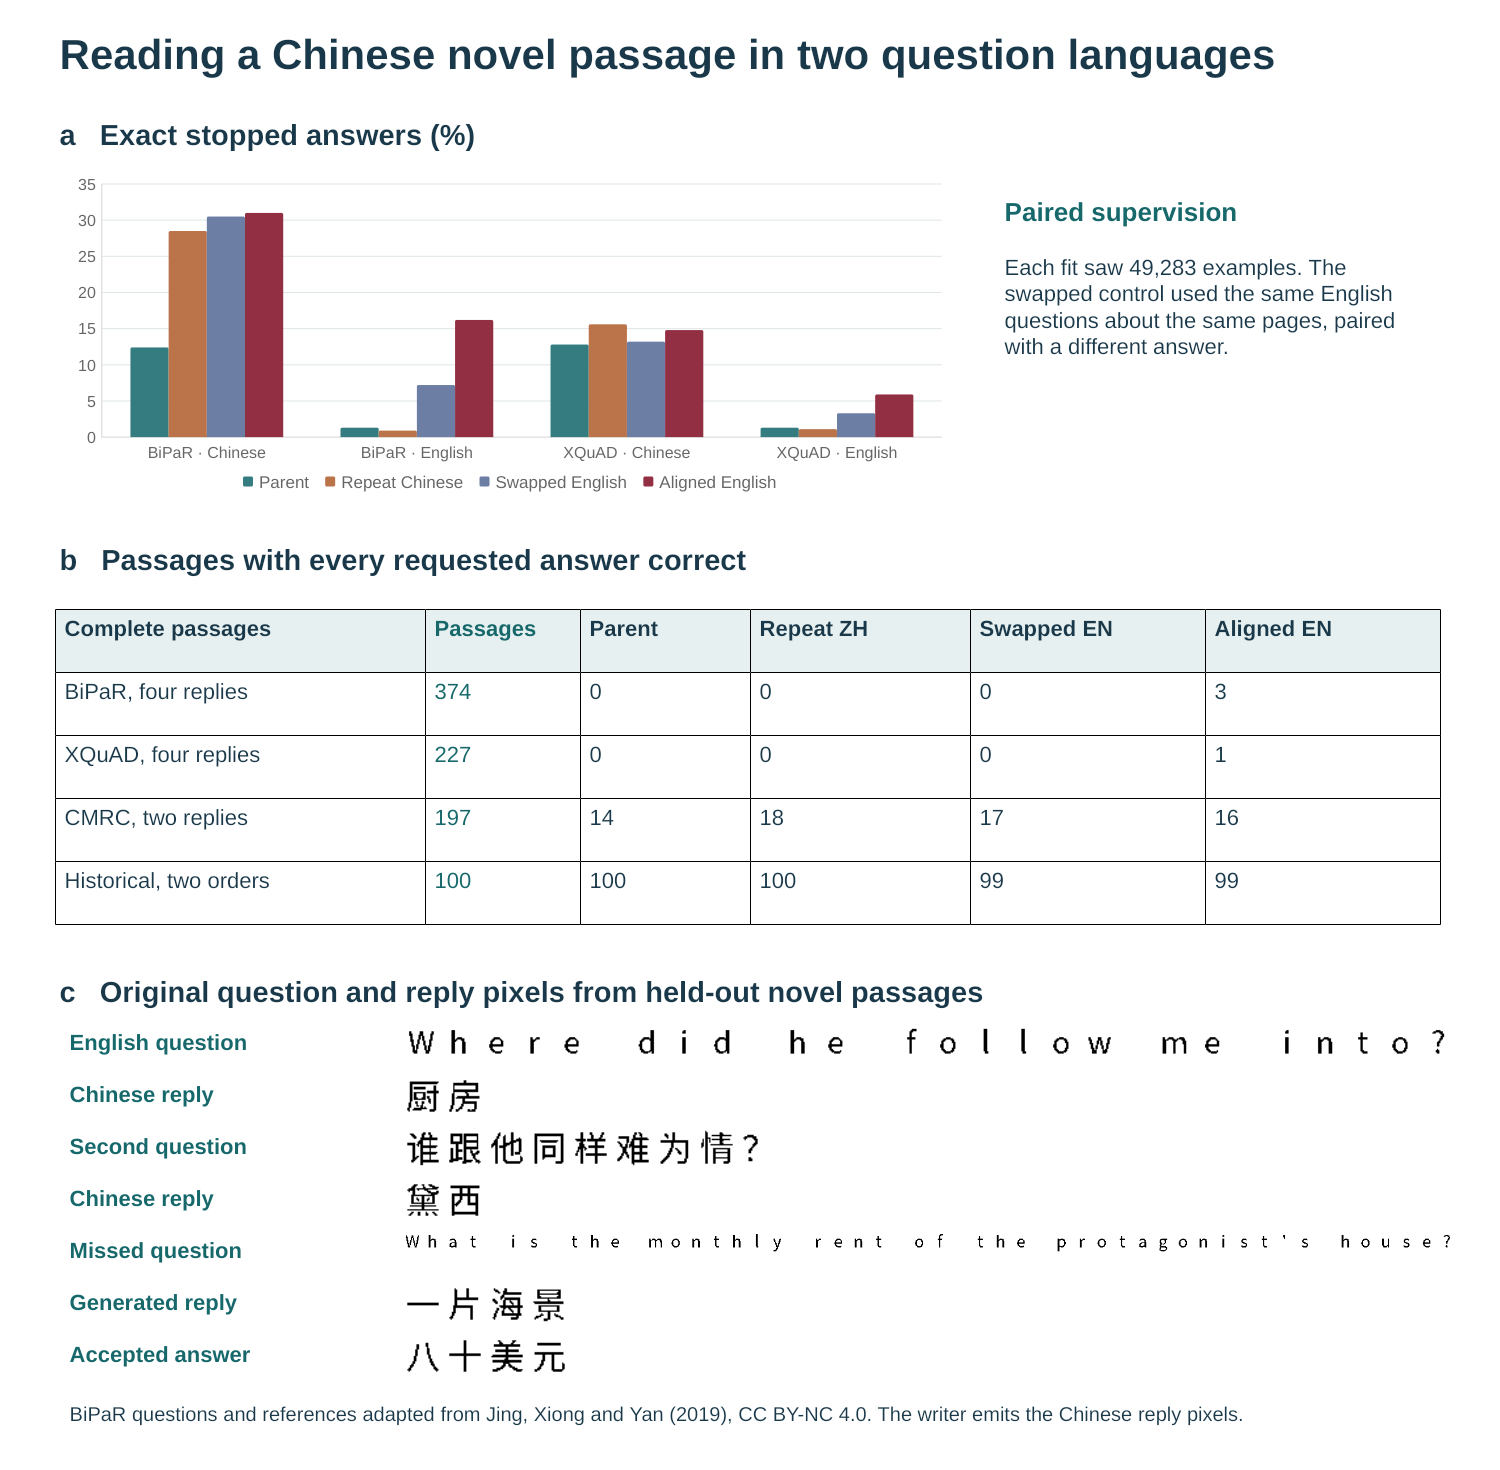
\includegraphics[width=.84\textwidth]{figures/Figure_104_bilingual_novel.png}
\caption{\DIFaddFL{\textbf{Bilingual question supervision on depicted Chinese passages.}
\textbf{a,} Exact stopped image replies to Chinese and English questions about Chinese novel passages from BiPaR and encyclopaedic passages from XQuAD. Bars show percentages for the parent and three fine-tuned writers. \textbf{b,} Complete passage counts require four answers for bilingual evaluations, both questions for CMRC and both requested orders for historical cards. \textbf{c,} Original question, reply and reference pixels from evaluation in source order. BiPaR questions and reference material are adapted from Jing, Xiong and Yan (2019) under CC BY-NC 4.0.}}
\label{fig:bilingual-novel}
\end{figure*}
\begin{figure*}[p]
\centering
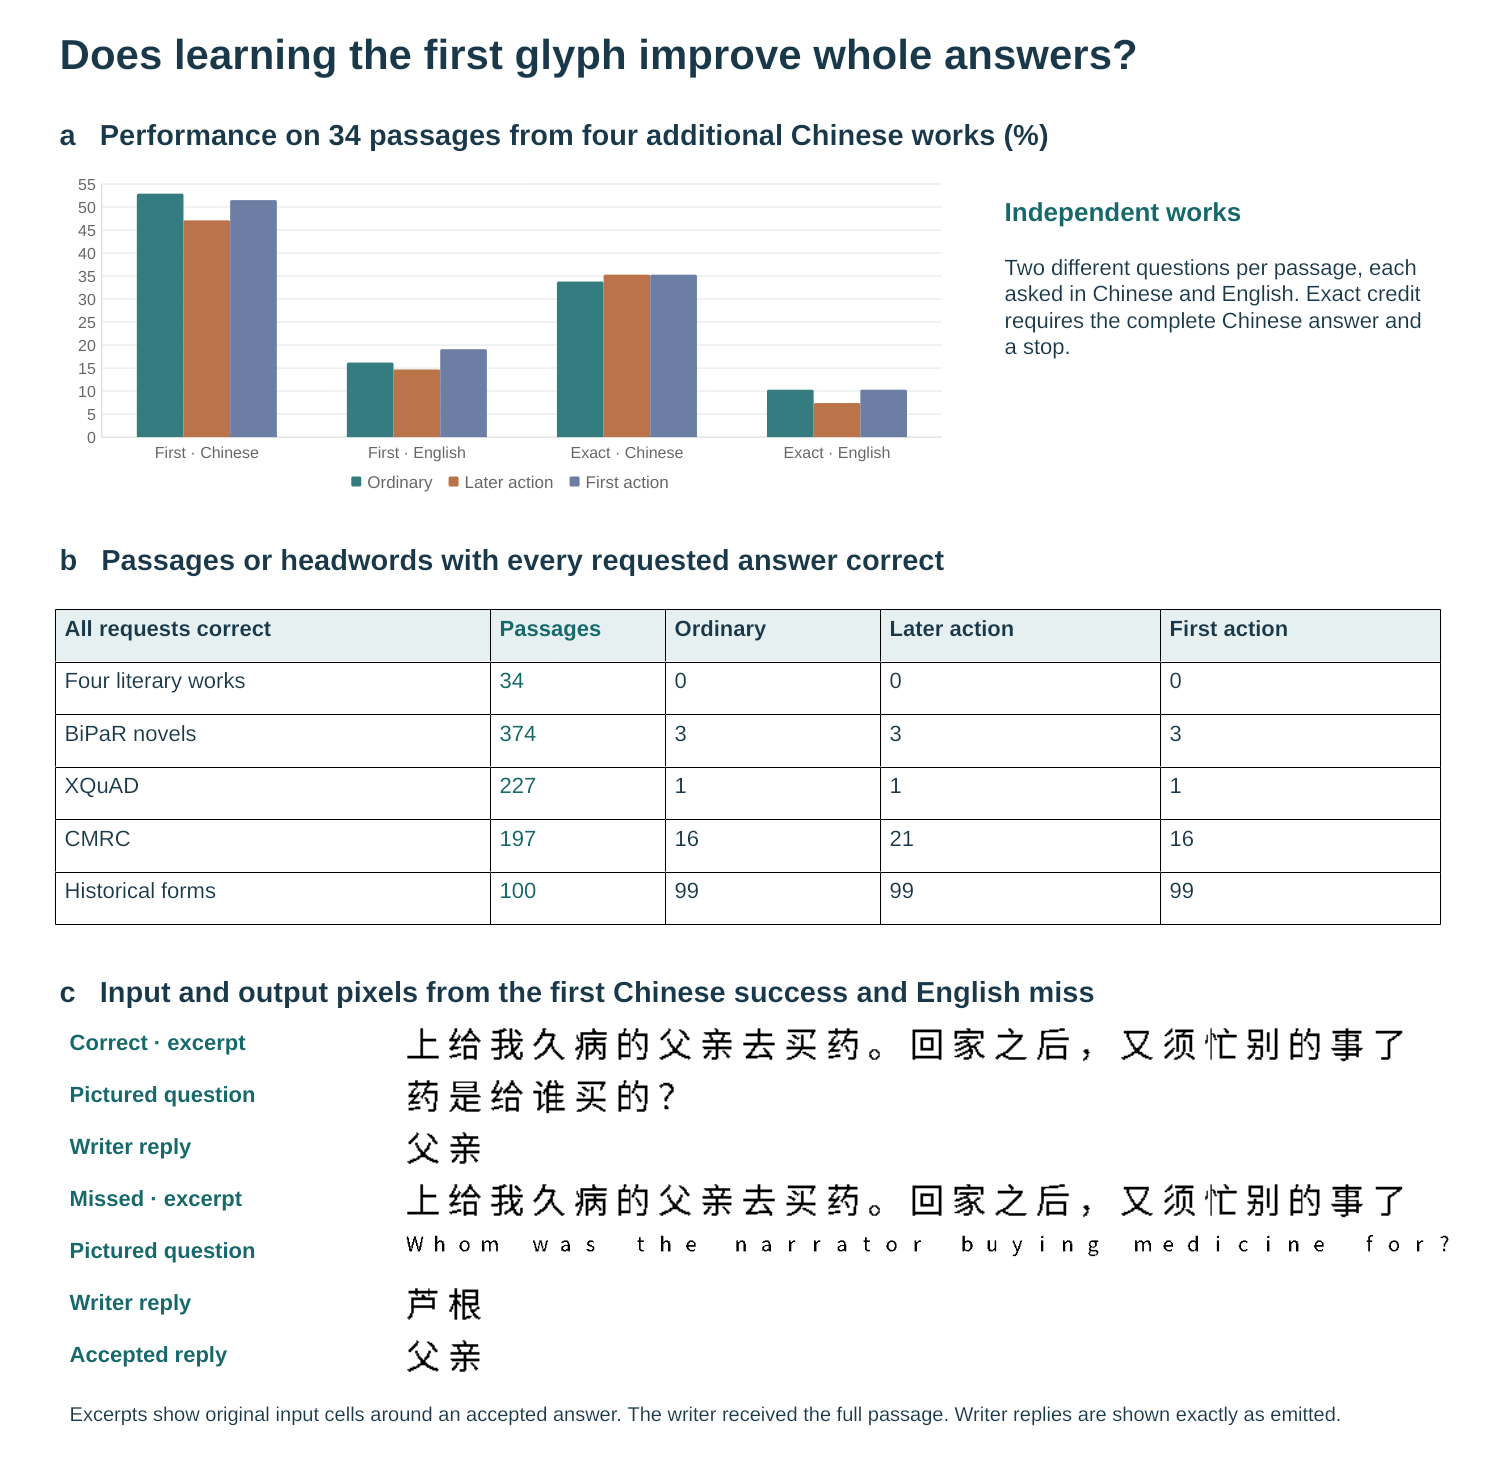
\includegraphics[width=.84\textwidth]{figures/Figure_105_first_glyph_book.png}
\caption{\DIFaddFL{\textbf{First-glyph supervision and complete answers on independent literary works.}
\textbf{a,} Correct initial glyph and exact stopped reply frequencies for 68 Chinese and 68 English requests. Each question refers to a Chinese passage. Bars compare ordinary bilingual supervision, additional supervision on a later action and additional supervision on the first action. \textbf{b,} Literary works, BiPaR and XQuAD require four correct answers per passage. CMRC and the historical headwords require two. \textbf{c,} Unmodified glyph pixels from the first exact Chinese reply and the first missed English reply in passage order for the first-action writer. Excerpts reproduce cells from the input around an accepted answer. The full passages were available at inference.}}
\label{fig:first-glyph-book}
\end{figure*}
\begin{figure*}[p]
\centering

\includegraphics[width=.84\textwidth]{figures/Figure_106_stopped_book_preference.png}
\caption{\DIFaddFL{\textbf{Learning to prefer a complete book answer and reading a new passage.}
\textbf{a,} Percentage of supervised pairs in which the complete annotated reply has greater joint probability than the released writer's earlier wrong reply. Shorter, equal and longer refer to the rival's length relative to the annotation. \textbf{b,} Passages or headwords with every required reply correct in free generation. Literary, BiPaR and XQuAD passages require four replies. CMRC passages and historical cards require two. \textbf{c,} Original input and reply pixels for the first exact Chinese-request reply and first nonempty missed English-request reply in reserved passage order. The excerpt locates an accepted answer on the full input page. The writer receives the full passage and question.}}
\label{fig:stopped-book-preference}
\end{figure*}
\begin{figure*}[p]
\centering
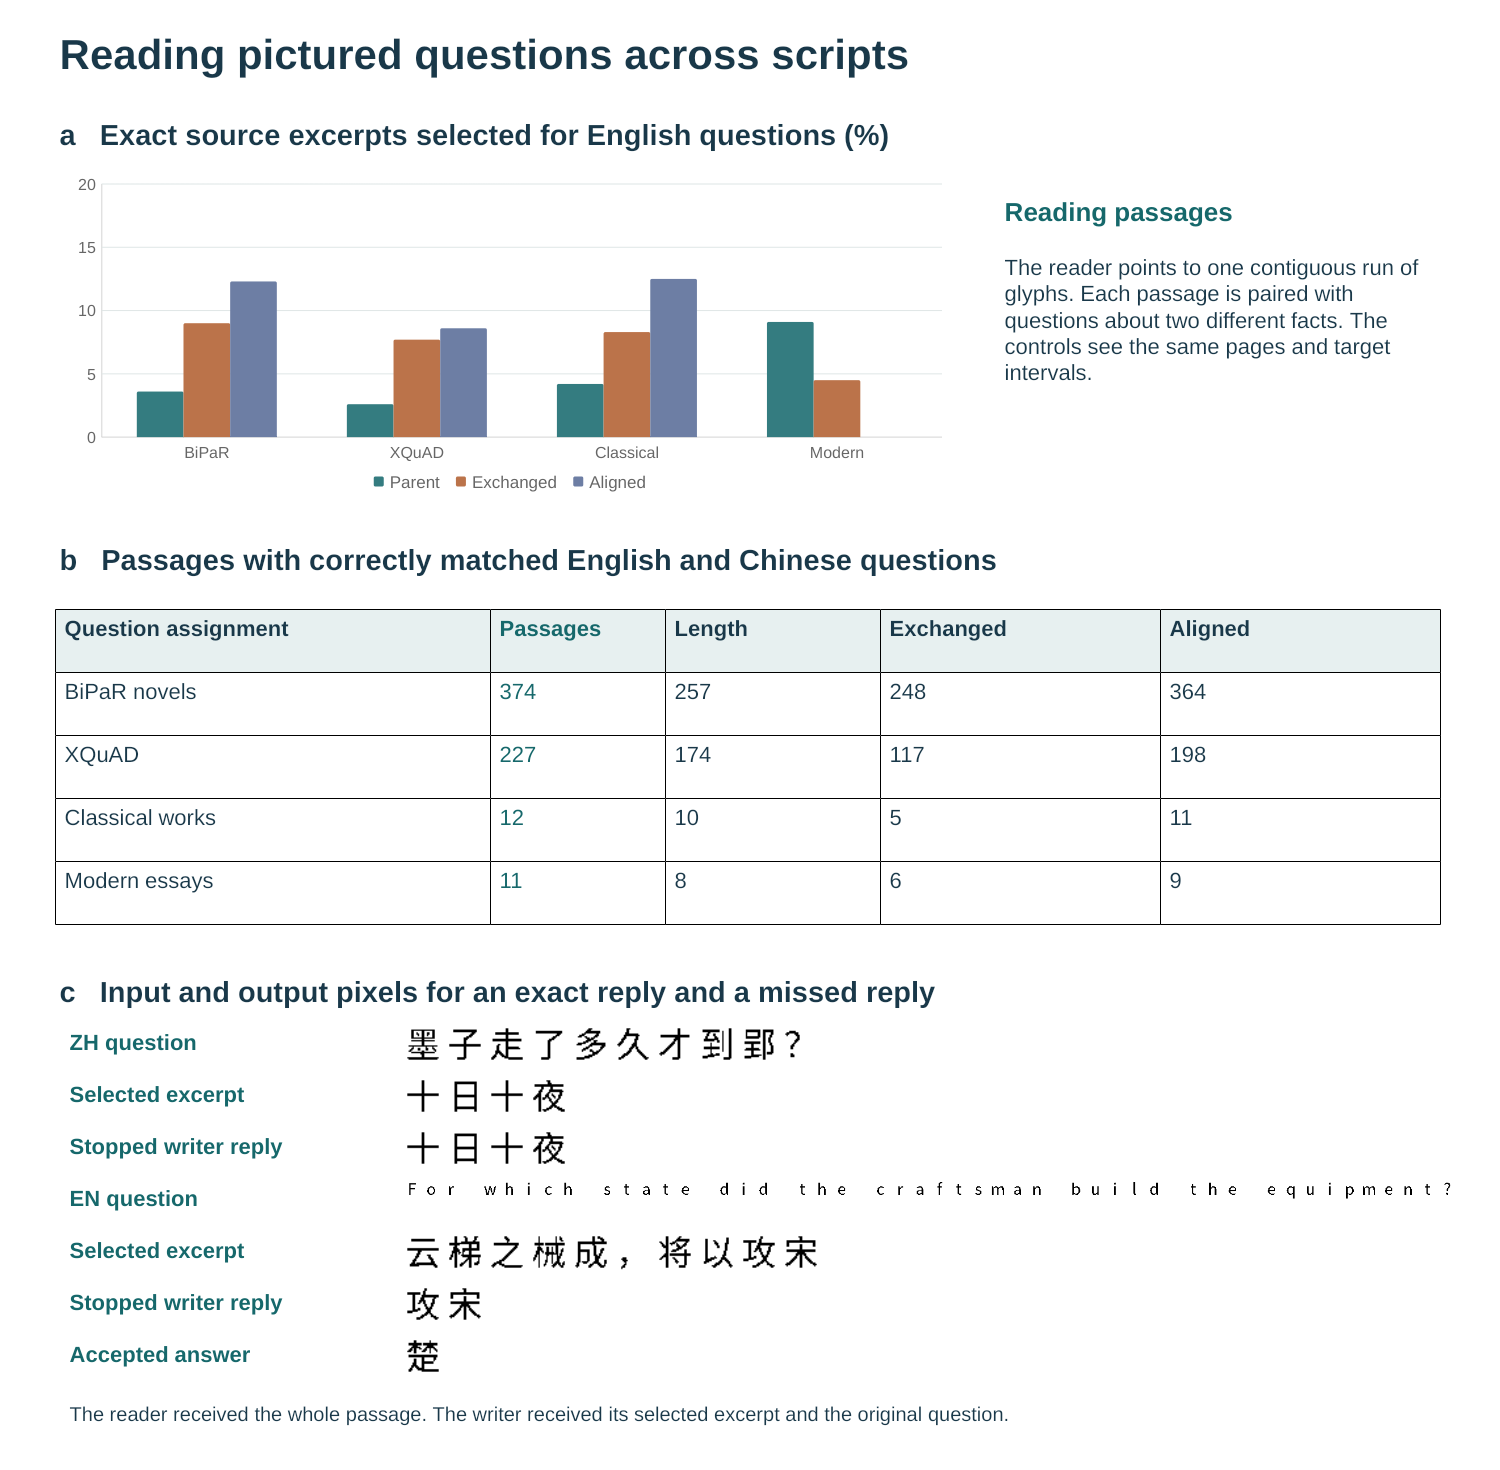
\includegraphics[width=.84\textwidth]{figures/Figure_107_bilingual_book_intervals.png}
\caption{\DIFaddFL{\textbf{Cross-script question identity and source reading.}
\textbf{a,} Exact pictured excerpts retrieved for English questions. BiPaR and XQuAD are previously evaluated development sources. The new classical and modern packets contain 24 and 22 English requests, respectively.
\textbf{b,} Strictly correct joint assignments of two English to two Chinese questions from the same passage. The separate visual question encoders receive only the four question images. Ties receive no credit. The length baseline compares the lengths of the two streams.
\textbf{c,} Original glyphs for the first exact Chinese-request reply and first nonempty missed English-request reply in fixed packet order. The writer emits its own cells and stop after receiving the predicted excerpt.}}
\label{fig:bilingual-book-intervals}
\end{figure*}
\begin{figure*}[p]
\centering
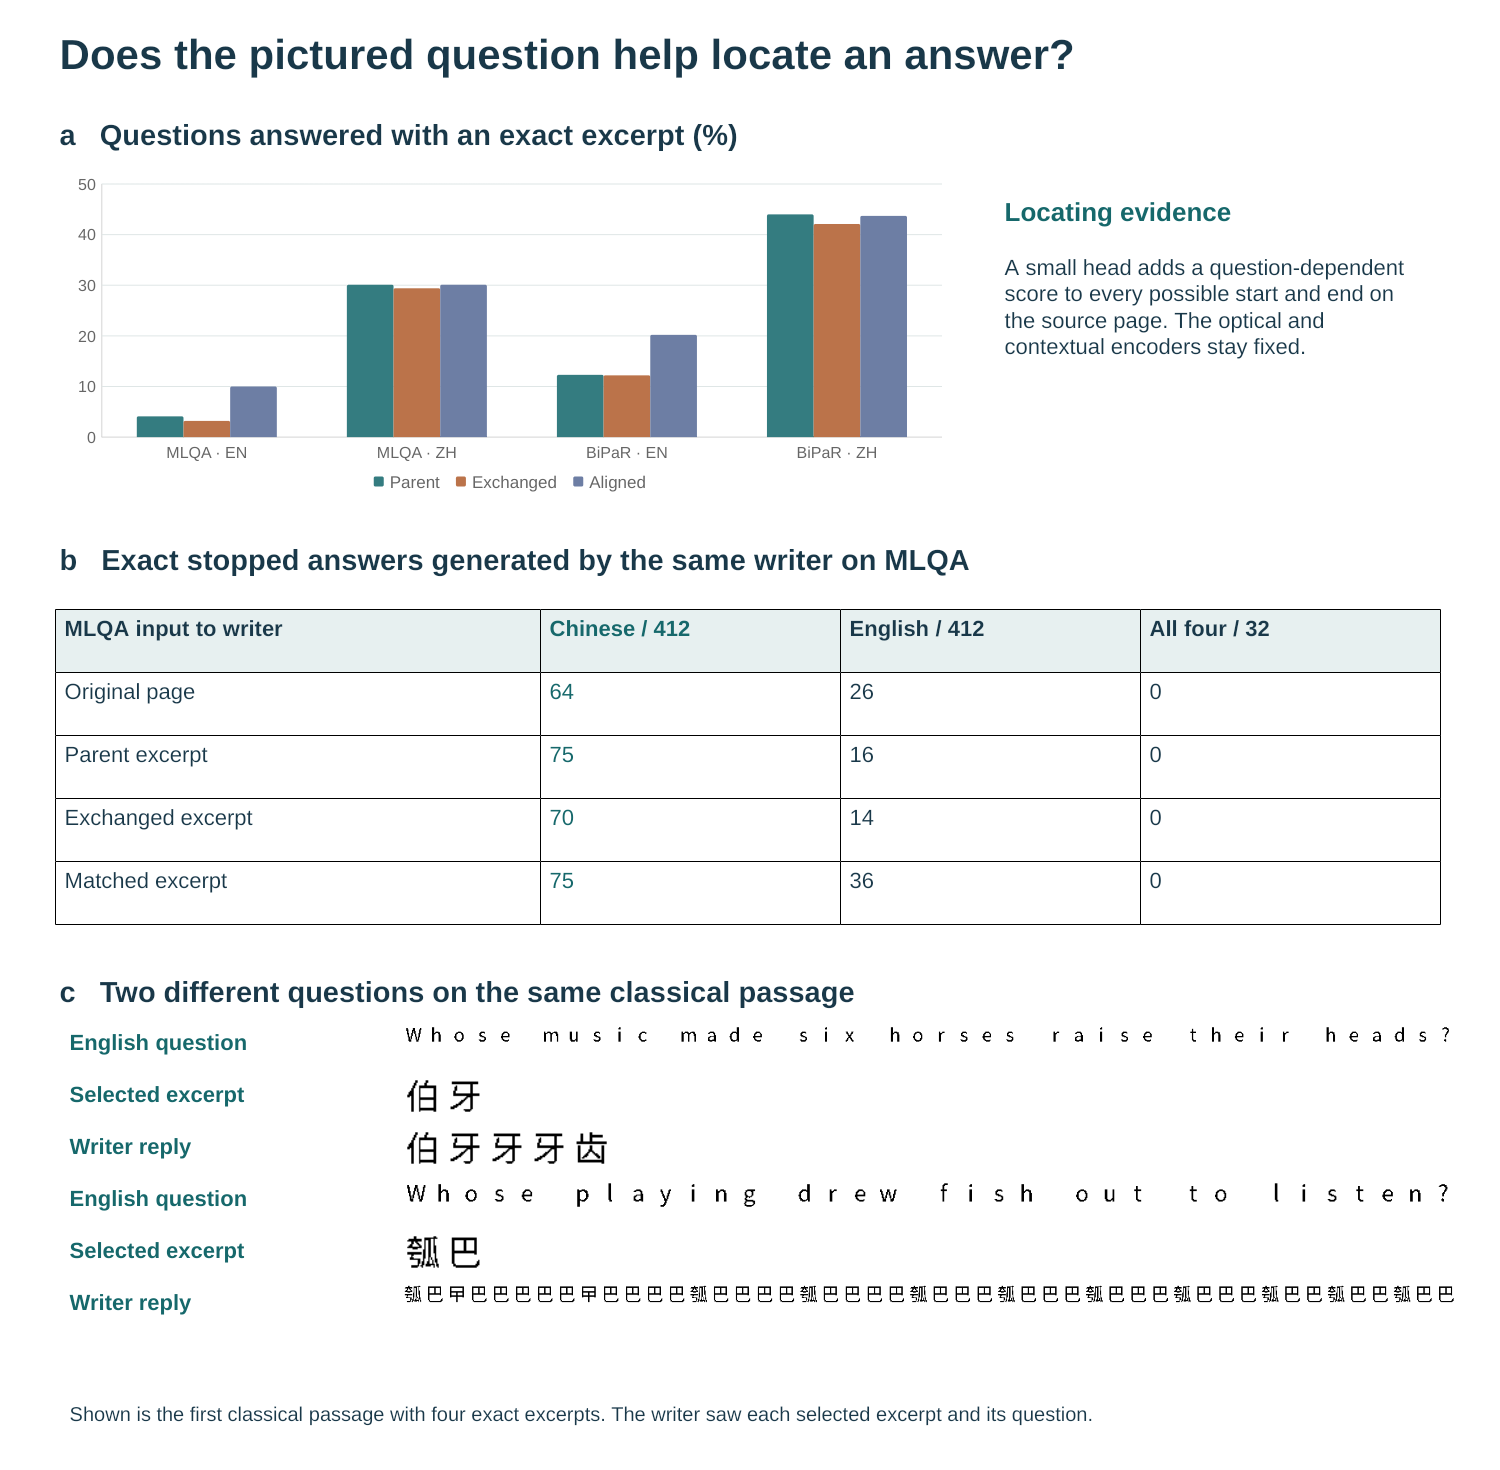
\includegraphics[width=.84\textwidth]{figures/Figure_108_question_evidence_transfer.png}
\caption{\DIFaddFL{\textbf{Using a cross-script question vector to locate and write a pictured answer.}
\textbf{a,} Exact excerpt rates on the Chinese-context MLQA development subset and the BiPaR novel development pages. EN and ZH denote the question language. Matched and exchanged fits add the same number of parameters to the frozen parent.
\textbf{b,} Exact freely stopped replies after presenting either the full original page or the predicted excerpt to the released causal writer, together with the actual question. The last column counts pages with two different facts answered in both languages.
\textbf{c,} Measured English question, selected source cells and writer output for two different facts on the first classical passage with four exact selections. Panels a and b include failures.
The selected names are correct under both English requests. The first generated reply stops incorrectly, and the second reaches the 48-cell limit.}}
\label{fig:question-evidence-transfer}
\end{figure*}
\begin{figure*}[p]
\centering
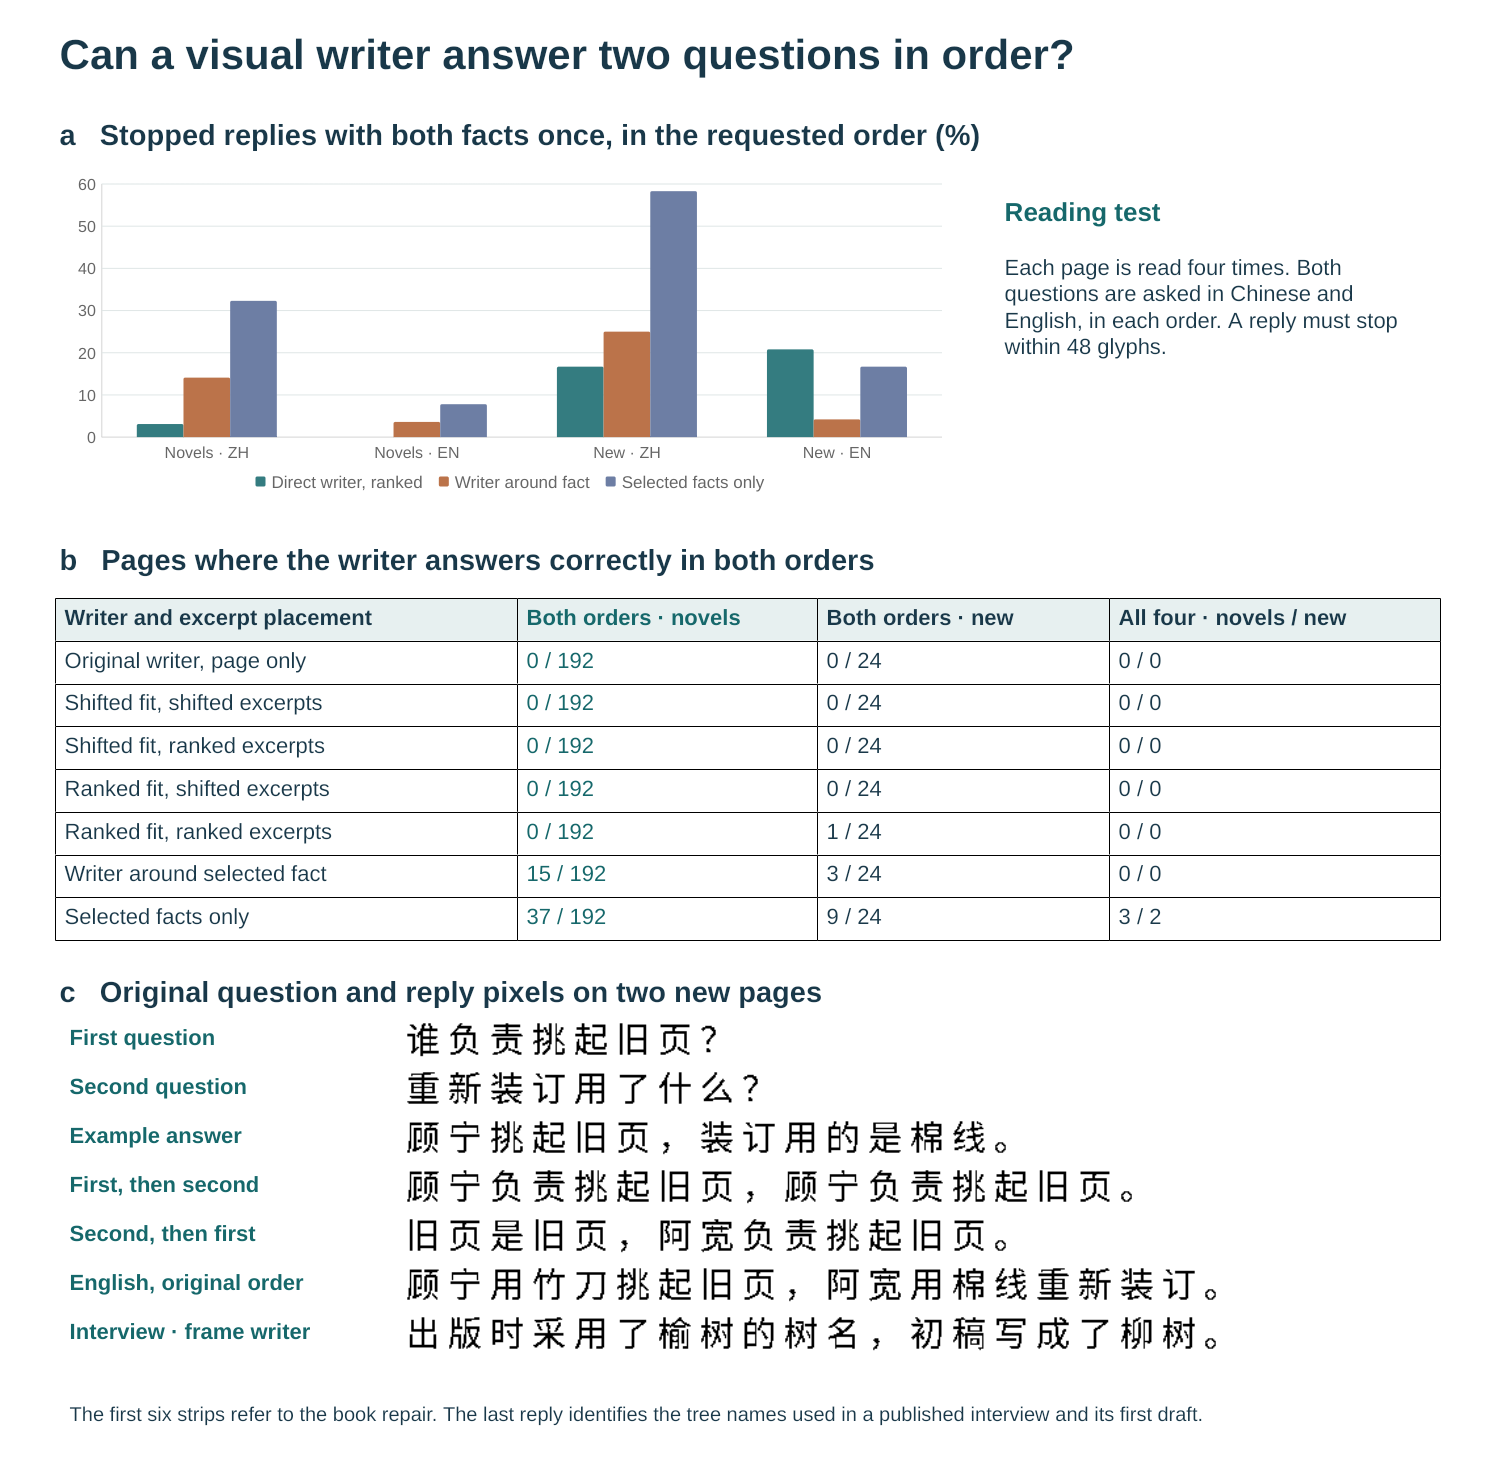
\includegraphics[width=.84\textwidth]{figures/Figure_109_ordered_book_replies.png}
\caption{\DIFaddFL{\textbf{Writing two answers from one pictured page.}
\textbf{a,} Percentage of freely stopped replies that include both specified facts exactly once and in the requested order. The direct writer receives ranked excerpts, the clause writer writes around a selected excerpt, and the list control joins the selected excerpts alone. Each novel-language group contains 192 requests and each new-page language group contains 24.
\textbf{b,} The central columns count page and language pairs where both orders received credit. The final column counts complete four-request pages out of 96 novel passages and 12 new passages, respectively.
\textbf{c,} Two Chinese questions about repairing a book on the first new page, one authored example answer and the full ranked writer's emitted strips. The two Chinese requests have opposite orderings. The third direct reply uses the corresponding English questions in the original order. The last strip is the clause writer's reply to the interview question on the twelfth new page, a selected success. A readable fact can still be assigned to the wrong action.}}
\label{fig:ordered-book-replies}
\end{figure*}
\begin{figure*}[p]
\centering
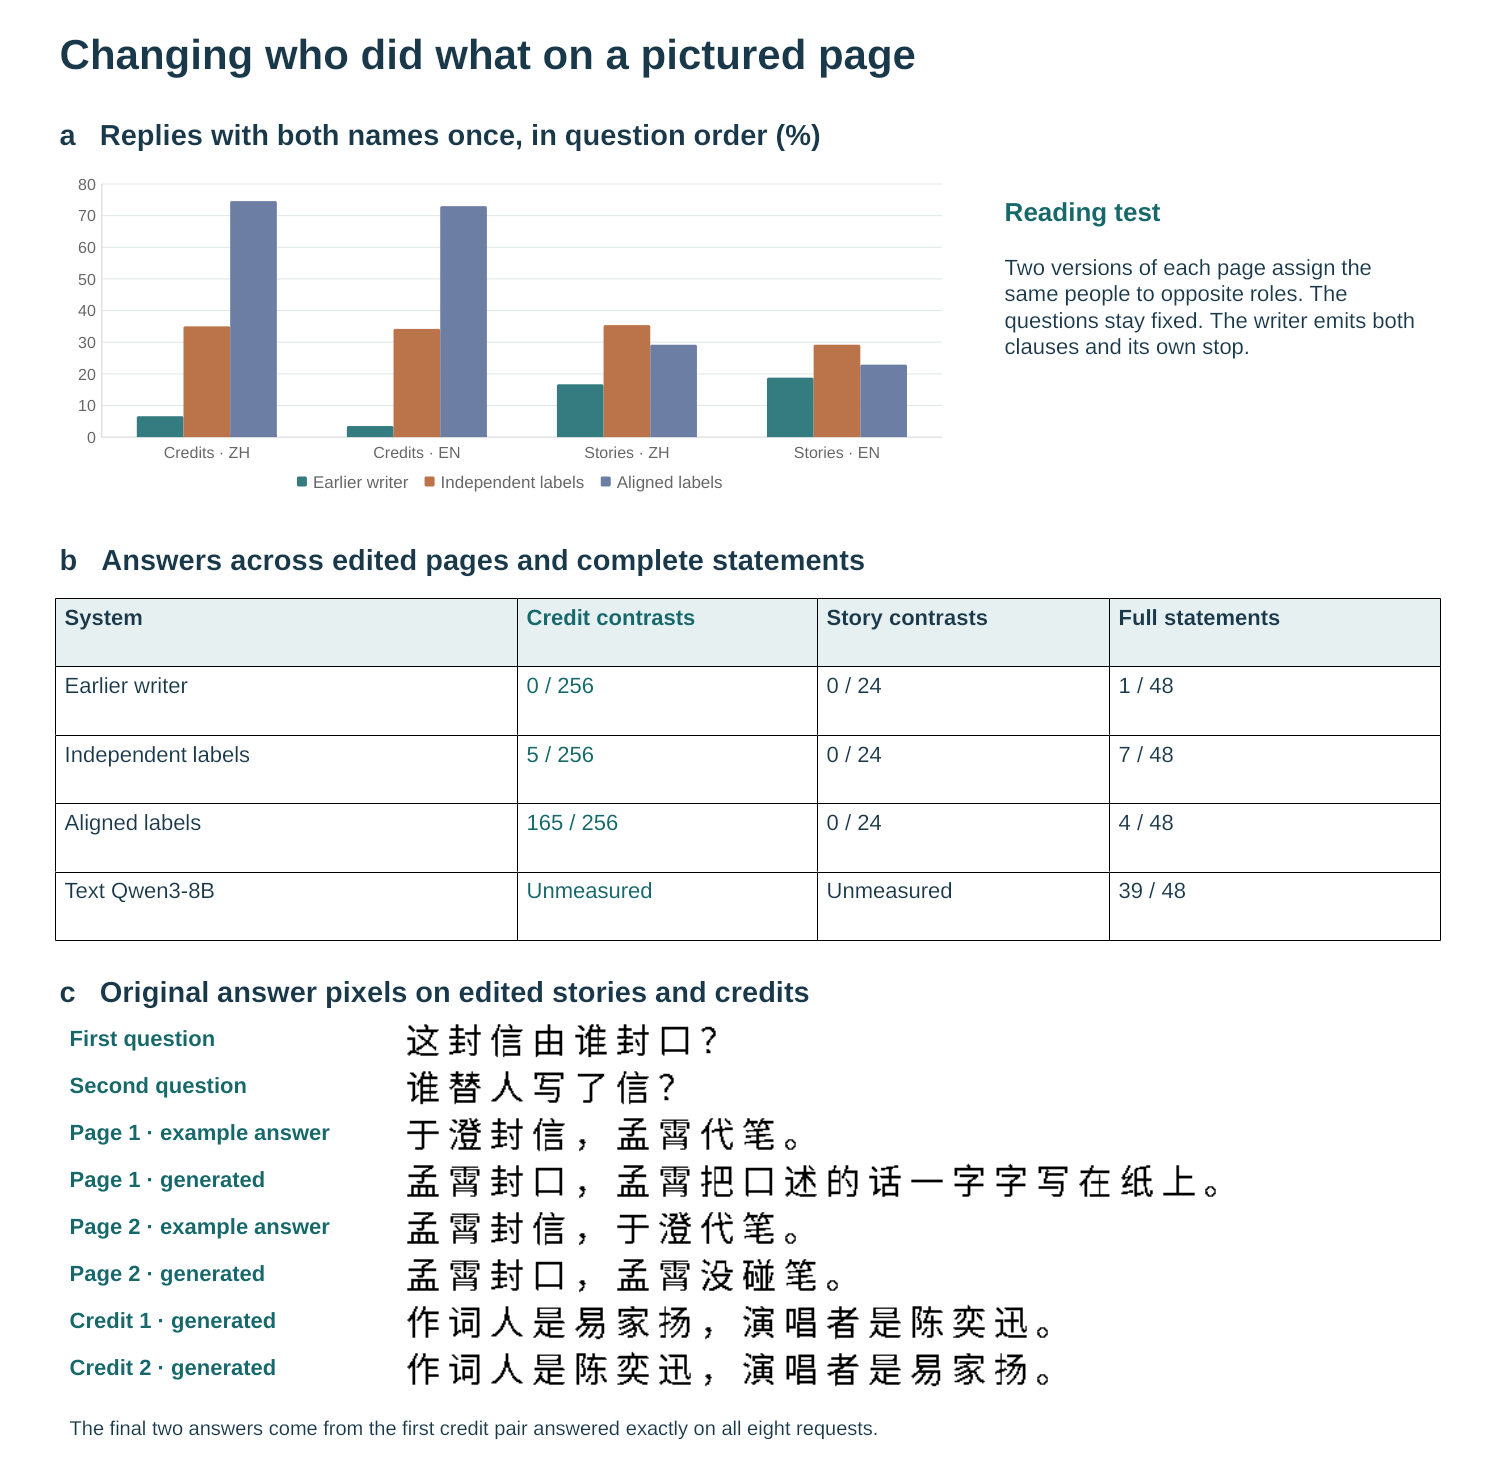
\includegraphics[width=.84\textwidth]{figures/Figure_110_role_change_writer.png}
\caption{\DIFaddFL{\textbf{Following an assignment across two pictured pages.}
\textbf{a,} Percentage of stopped replies containing both names exactly once in the requested order, for 512 requests per language on edited credits and 48 per language on independently worded stories. Aligned and independent-label writers saw the same inputs and answer counts.
\textbf{b,} A complete contrast requires success on both page versions in both question orders within a language. The last column counts complete supported statements in an arm-hidden reading on 48 story requests. The text system answered the manual reading sample.
\textbf{c,} The two Chinese questions and both answer images on the first registered story. One person seals a letter while the other writes it from dictation. The second version exchanges their assignments. Each generated strip preserves the writer's original pixels. The two example answers give possible correct wordings. The last two strips come from the first held-out credit pair on which all eight replies matched the annotated wording. The page identifies a lyricist and a singer; the experimental edit exchanges their names.}}
\label{fig:role-change-writer}
\end{figure*}
\begin{figure*}[p]
\centering
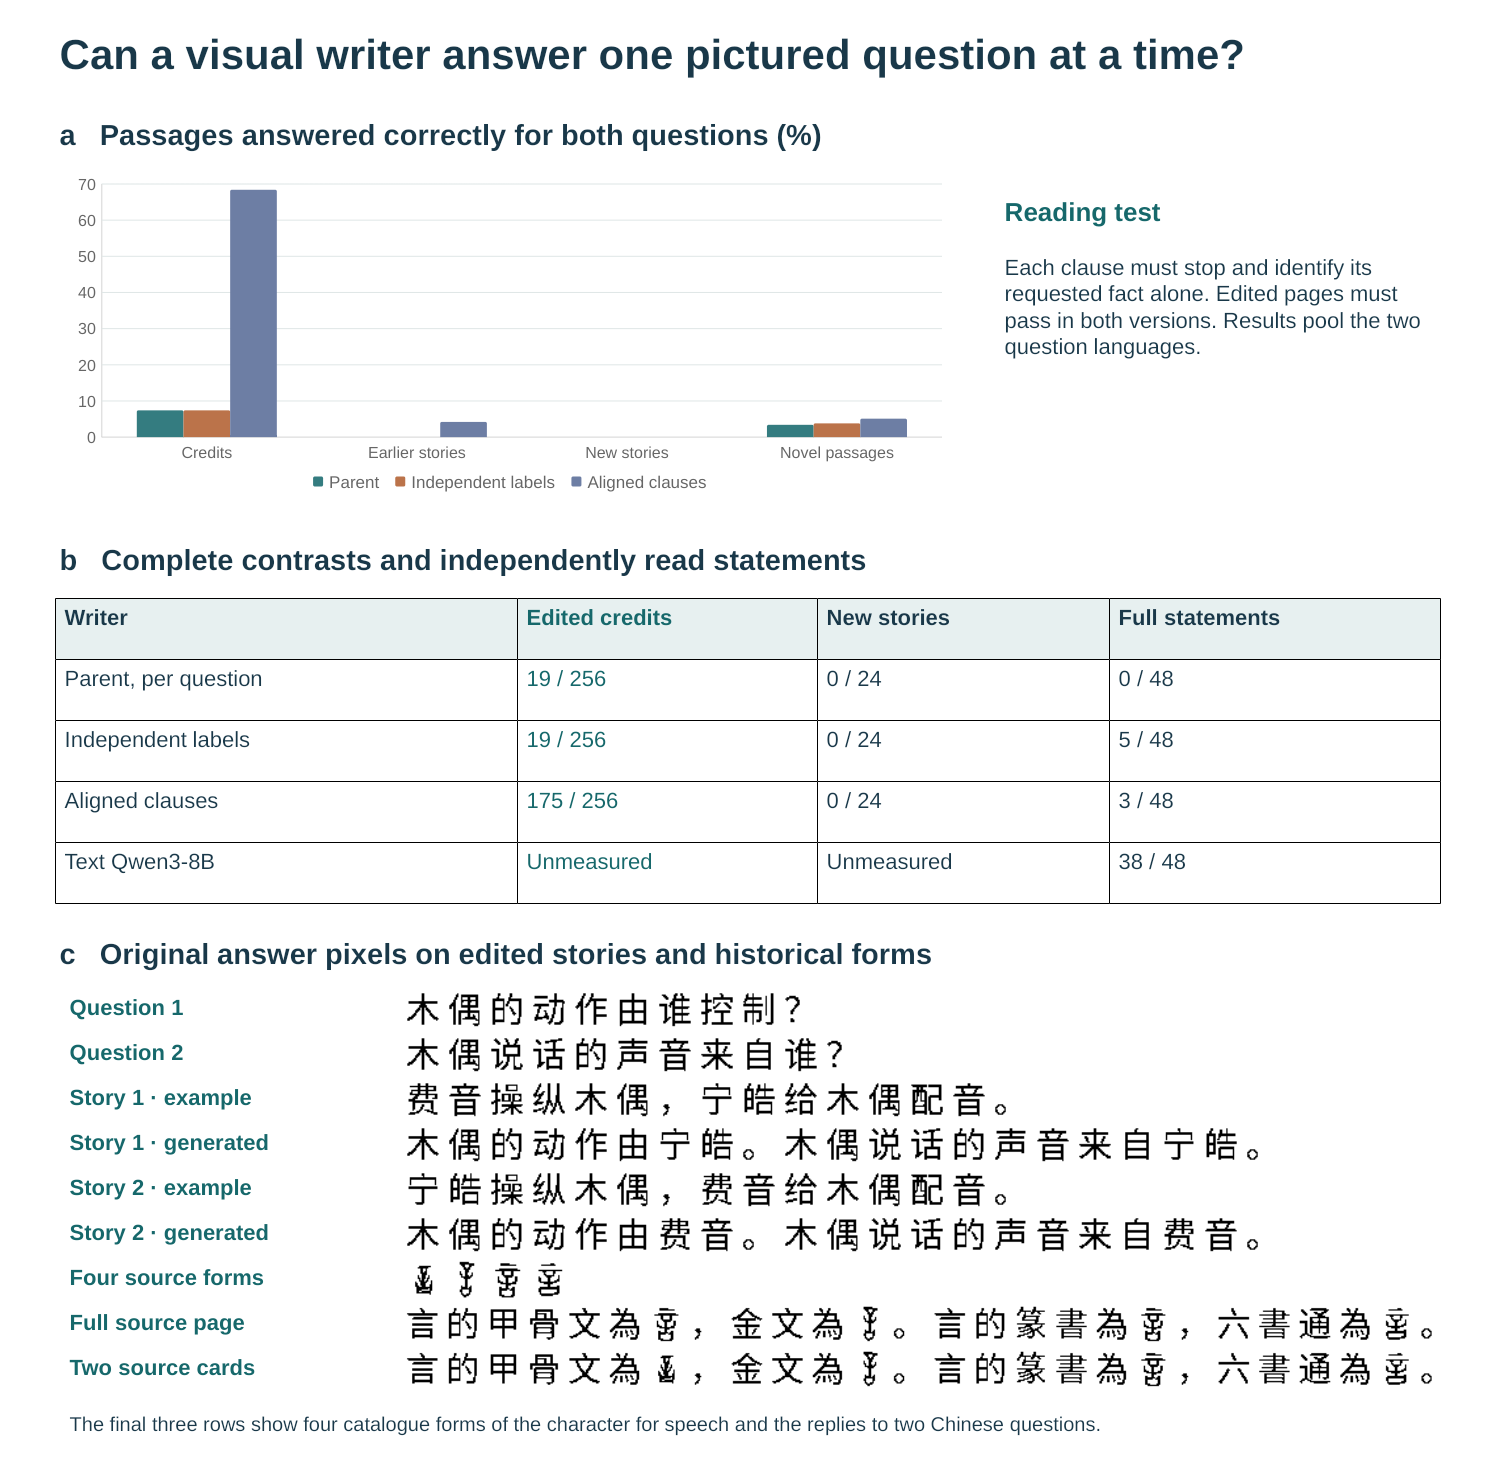
\includegraphics[width=.84\textwidth]{figures/Figure_111_individual_clause_writer.png}
\caption{\DIFaddFL{\textbf{Answering questions individually on pictured passages.}
\textbf{a,} Percentage of passage--language comparisons where both answers identify their requested fact and end. The credit and story groups also require success after the two participants exchange assignments. The novel group contains the 253 additional validation passages. Separate generation supplies the question order by construction.
\textbf{b,} The credit and new-story columns give the complete comparison counts. The last column reports supported full responses for the prespecified 48-request reading sample with system identities hidden.
\textbf{c,} Original question and answer pixels on the first new story. In the first account one person controls a puppet and another supplies its voice. Their roles exchange in the second. Each generated strip displays the two complete outputs consecutively. The final three rows show four catalogued forms of the character for speech and the generated replies to two Chinese questions. The full page displays all four categories. In the source-assisted condition, each question receives a card containing its two requested categories.}}
\label{fig:individual-clause-writer}
\end{figure*}
\begin{figure*}[p]
\centering
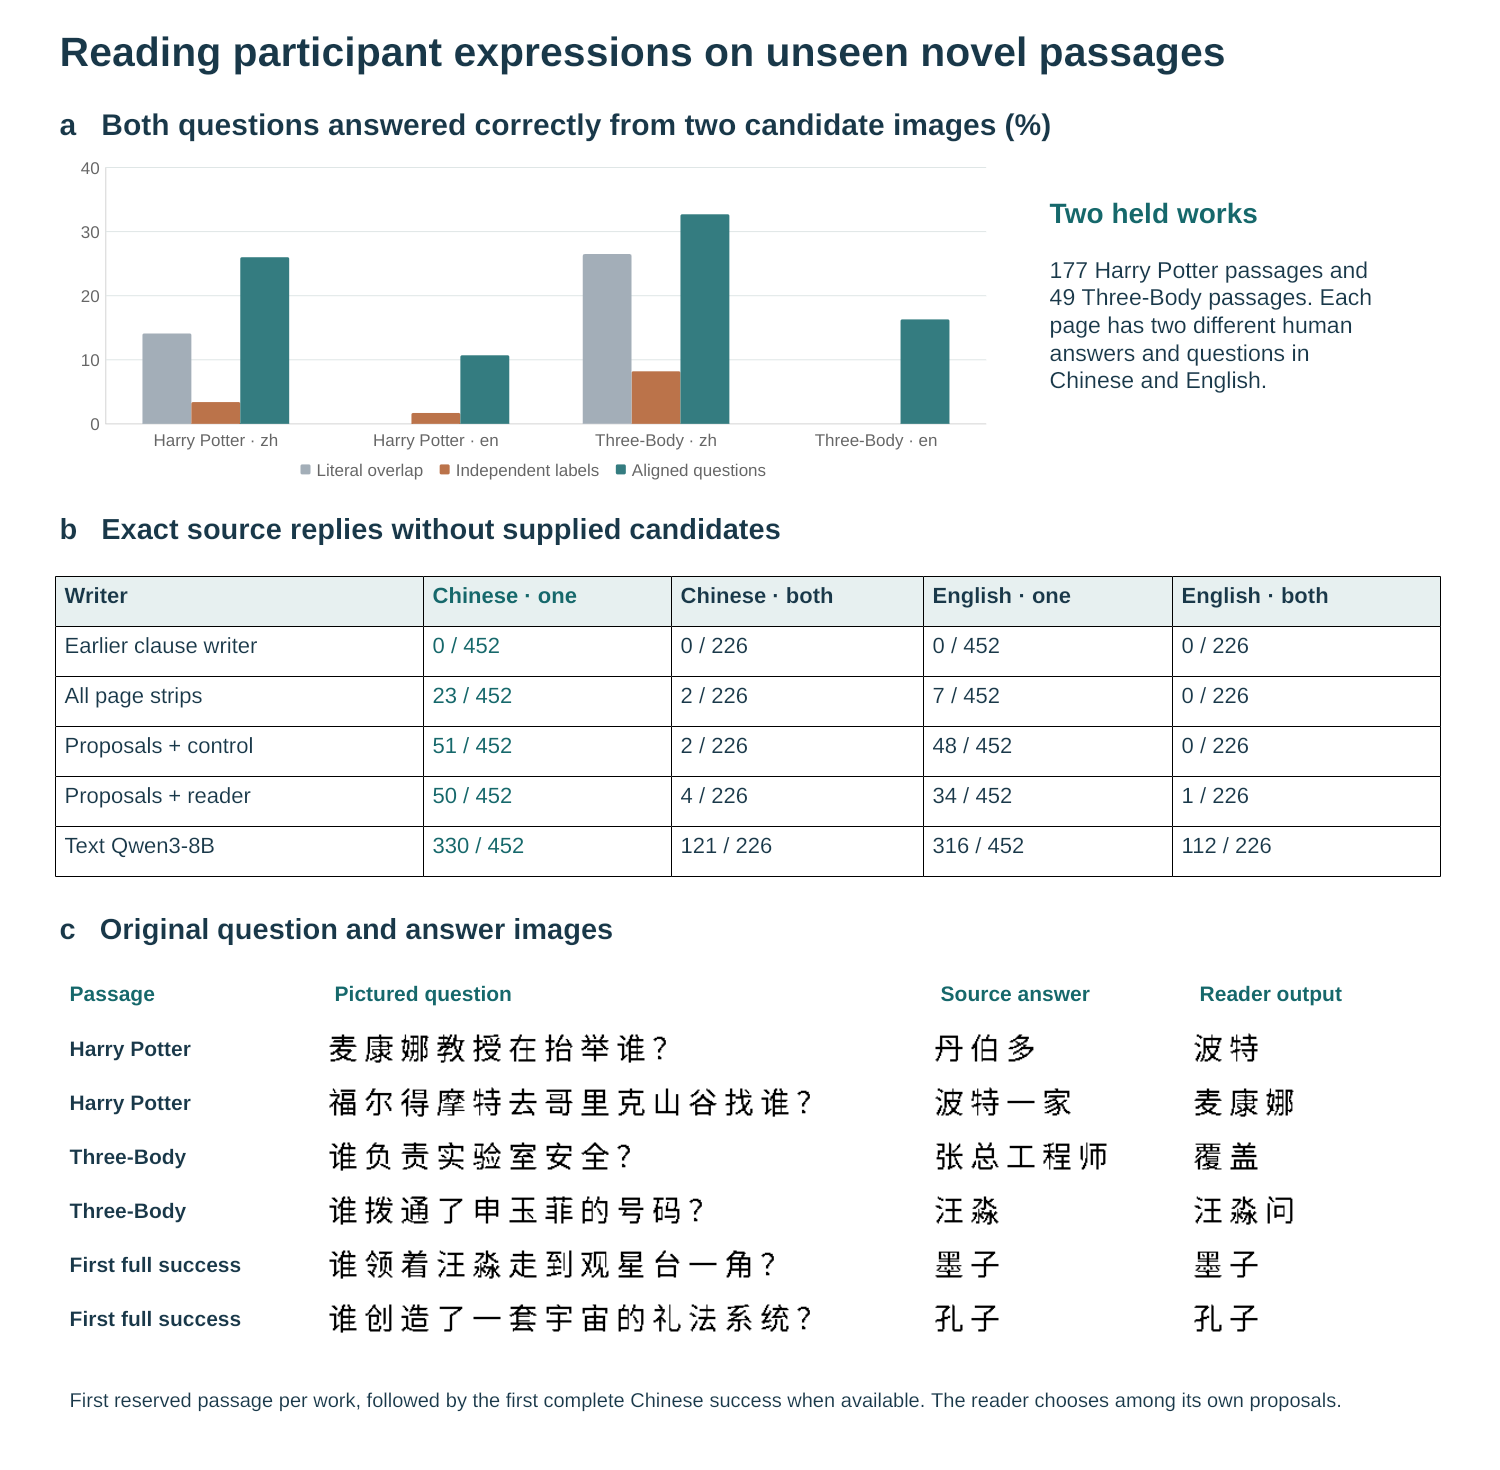
\includegraphics[width=.84\textwidth]{figures/Figure_112_book_participant_reader.png}
\caption{\DIFaddFL{\textbf{Identifying people in novels from pictured questions.}
\textbf{a,} Both answers must be correct when the reader chooses between the two annotated expressions in either candidate order. The novels were held out of training for the fresh readers. Chinese and English questions refer to the same Chinese passage. \textbf{b,} Individual exact image replies and completely answered passages with no candidate supplied at inference. The detector proposes up to 16 distinct source images. Text Qwen3-8B receives the printed content as text. Its response must stop and match the same reference. \textbf{c,} Original pixels of the Chinese questions, source answers and autonomous outputs from the detector and aligned reader. The first two questions per work follow the reserved source order. The final two show the first passage on which both Chinese answers were correct, selected to illustrate a success.}}
\label{fig:book-participant-reader}
\end{figure*}
\begin{figure*}[p]
\centering
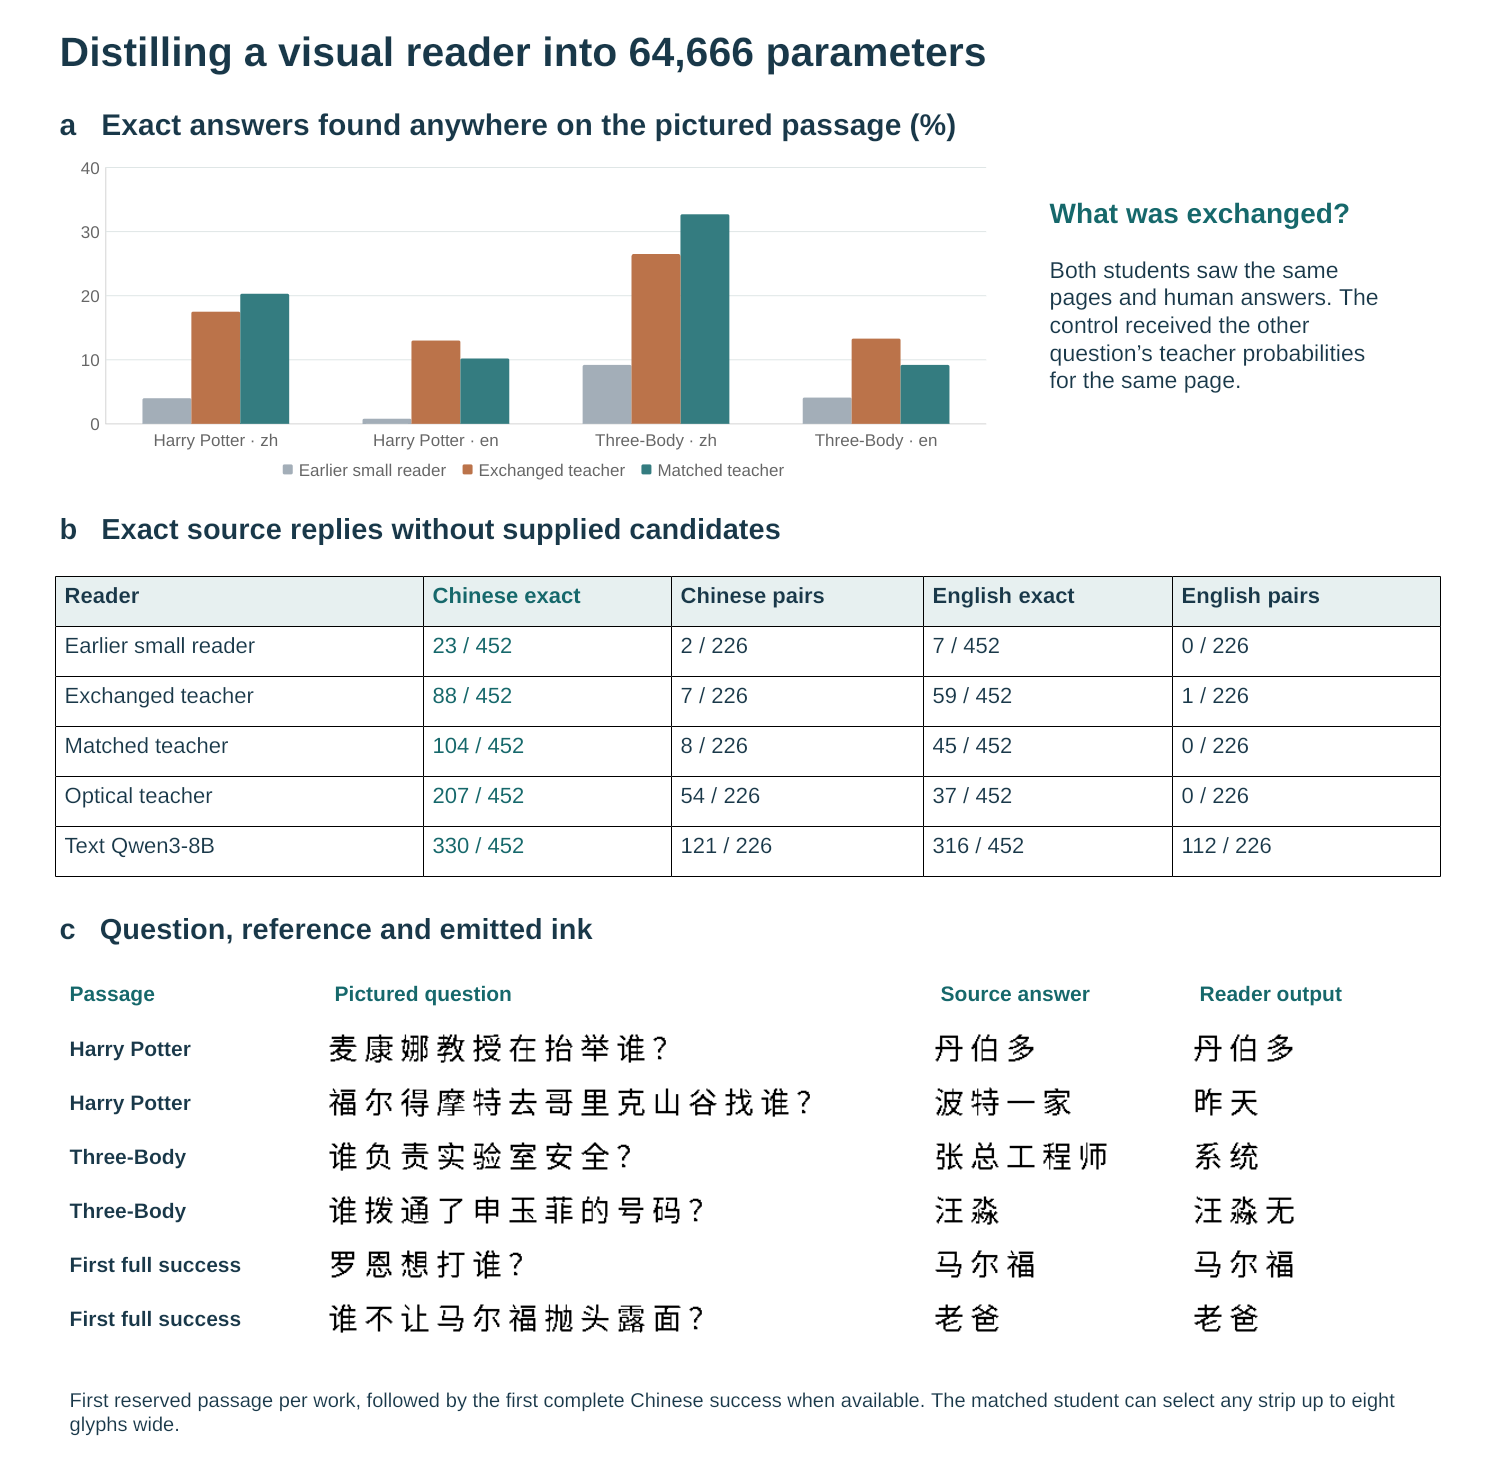
\includegraphics[width=.84\textwidth]{figures/Figure_113_book_span_distillation.png}
\caption{\DIFaddFL{\textbf{Transferring interval probabilities from a visual teacher.}
\textbf{a,} Exact source-image answers for each reserved novel and question language. Each question can select any contiguous strip of one to eight glyphs. The two students share the same human answer images. In the exchanged condition, the teacher distribution belongs to the other question about the same page. \textbf{b,} Exact answers to individual questions and to both questions about a passage. The optical teacher and text Qwen3-8B were evaluated on the same questions. \textbf{c,} Pictured questions, source answers and output bitmaps for the first reserved passage of each work. The final pair illustrates the first passage on which the matched student answered both Chinese questions correctly. All outputs are reproduced at their stored resolution before display scaling.}}
\label{fig:book-span-distillation}
\end{figure*}
\begin{figure*}[p]
\centering
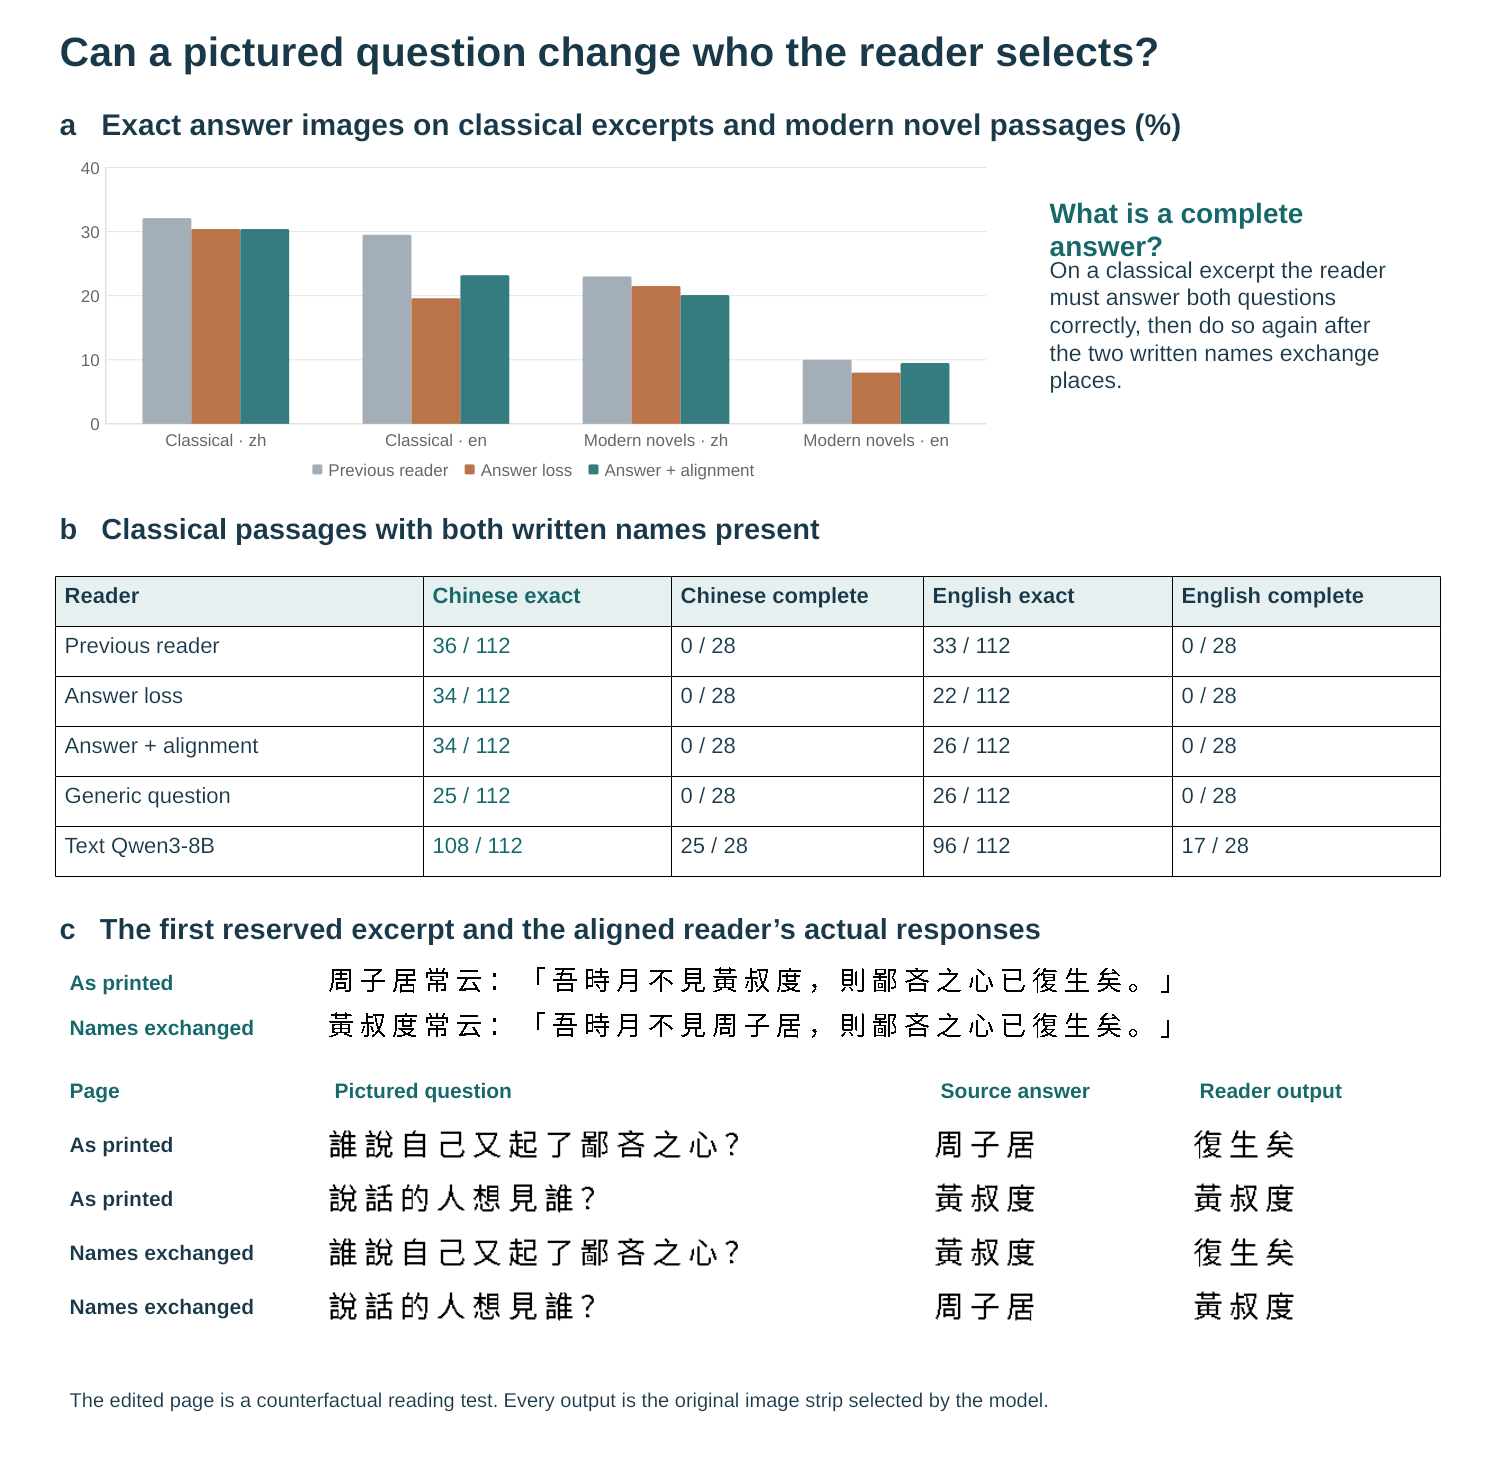
\includegraphics[width=.84\textwidth]{figures/Figure_114_role_question_binding.png}
\caption{\DIFaddFL{\textbf{Question alignment in classical prose.}
\textbf{a,} Individual short answers found freely on 28 classical excerpts and on 226 modern novel passages. Each of the classical originals also has a counterfactual version with the two names exchanged. \textbf{b,} A complete contrast requires four correct outputs in one language: both people on the original passage and both on the edited passage. All readers have access to the entire pictured passage. The text reference is a locally evaluated Qwen3-8B. \textbf{c,} Actual Chinese questions and original output pixels for the first source excerpt, reproduced for both assignments. The two fixed names and their order in the output columns allow inspection of partial successes and errors.}}
\label{fig:role-question-binding}
\end{figure*}
\begin{figure*}[p]
\centering
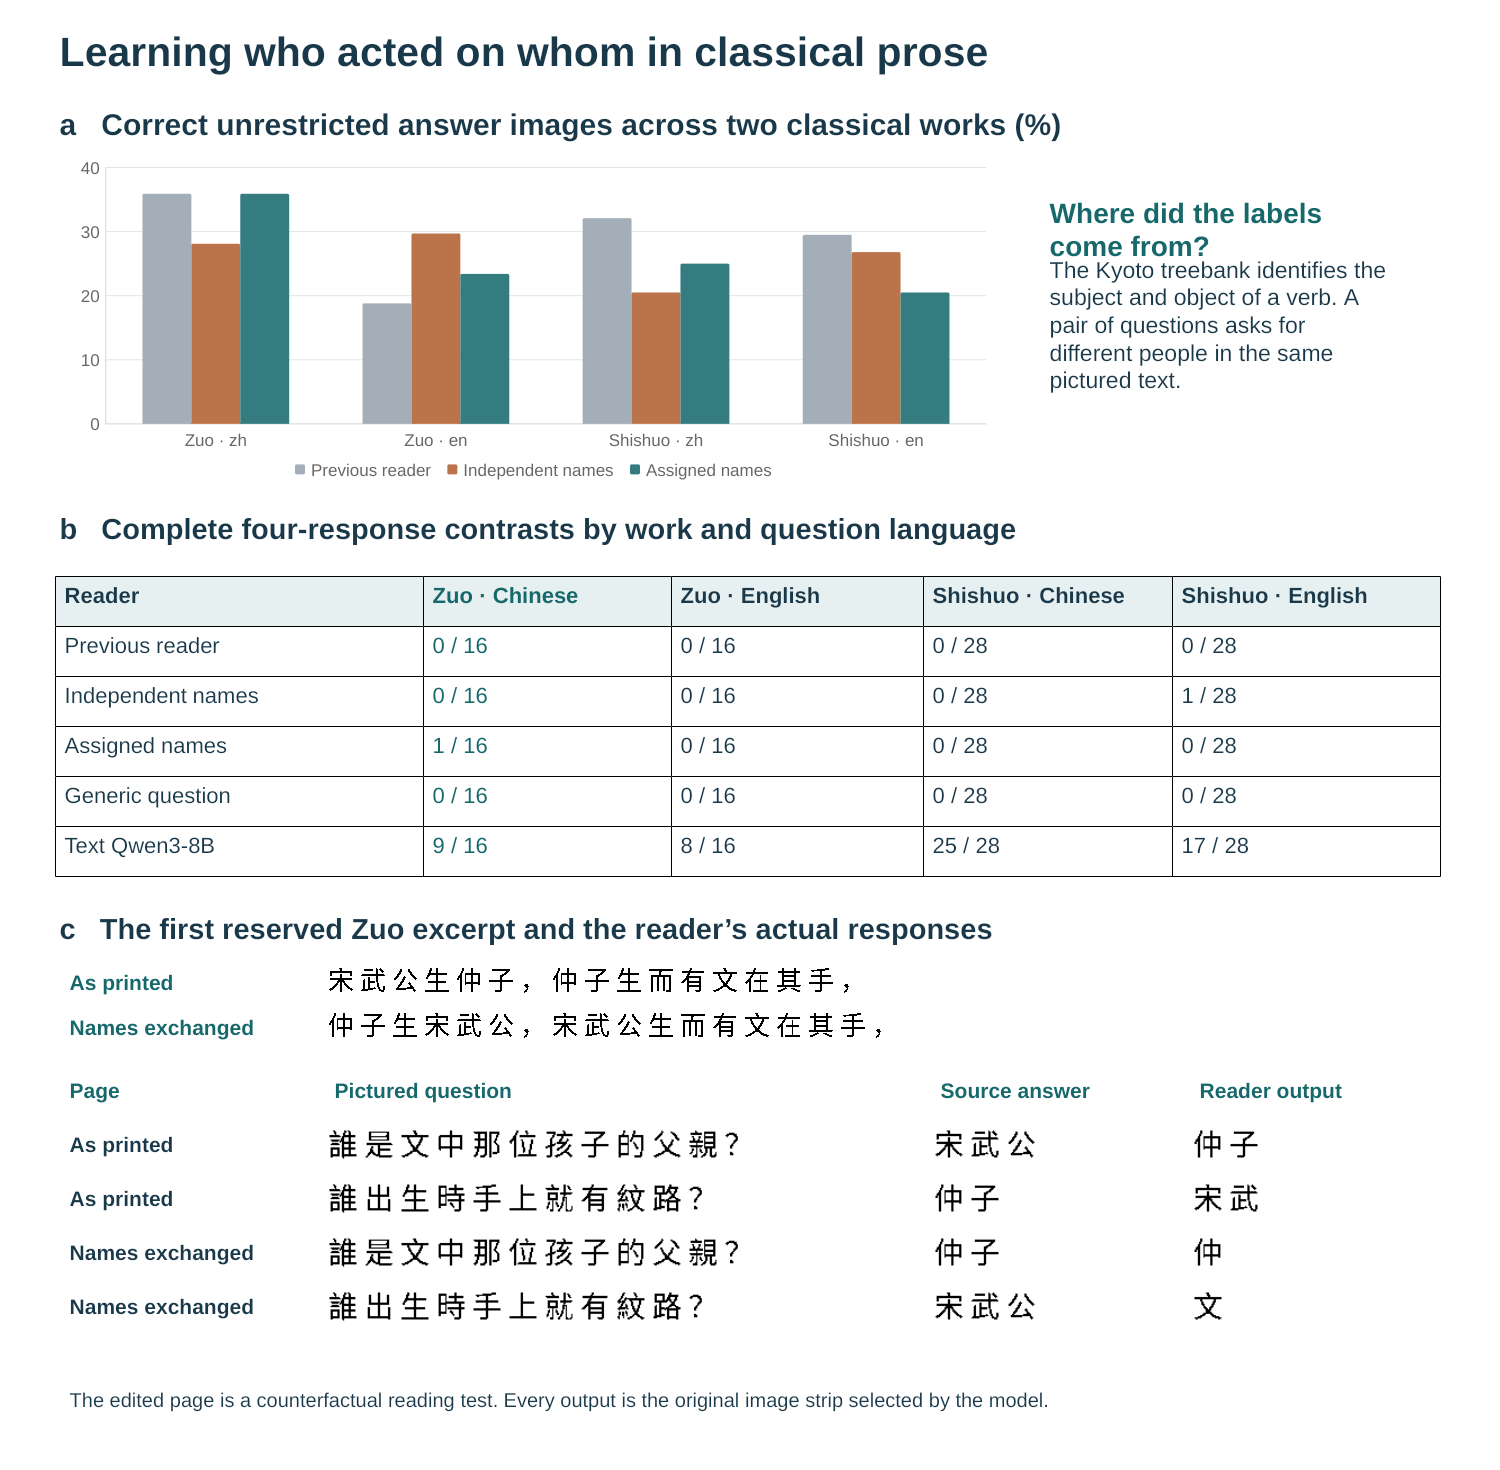
\includegraphics[width=.84\textwidth]{figures/Figure_115_classical_argument.png}
\caption{\DIFaddFL{\textbf{Identifying arguments in classical prose.}
\textbf{a,} Unrestricted exact source images for the two classical works and two question languages. \textbf{b,} Complete contrasts require both requested people in both the original and the name-exchanged passage. The two small updated readers start at the released visual reader and see the same supervised images in aggregate. \textbf{c,} The first prospectively reserved excerpt from the \textit{Zuo Tradition} and its marked counterfactual, with the corresponding questions, reference images and original outputs from the aligned reader.}}
\label{fig:classical-argument}
\end{figure*}
\begin{figure*}[p]
\centering
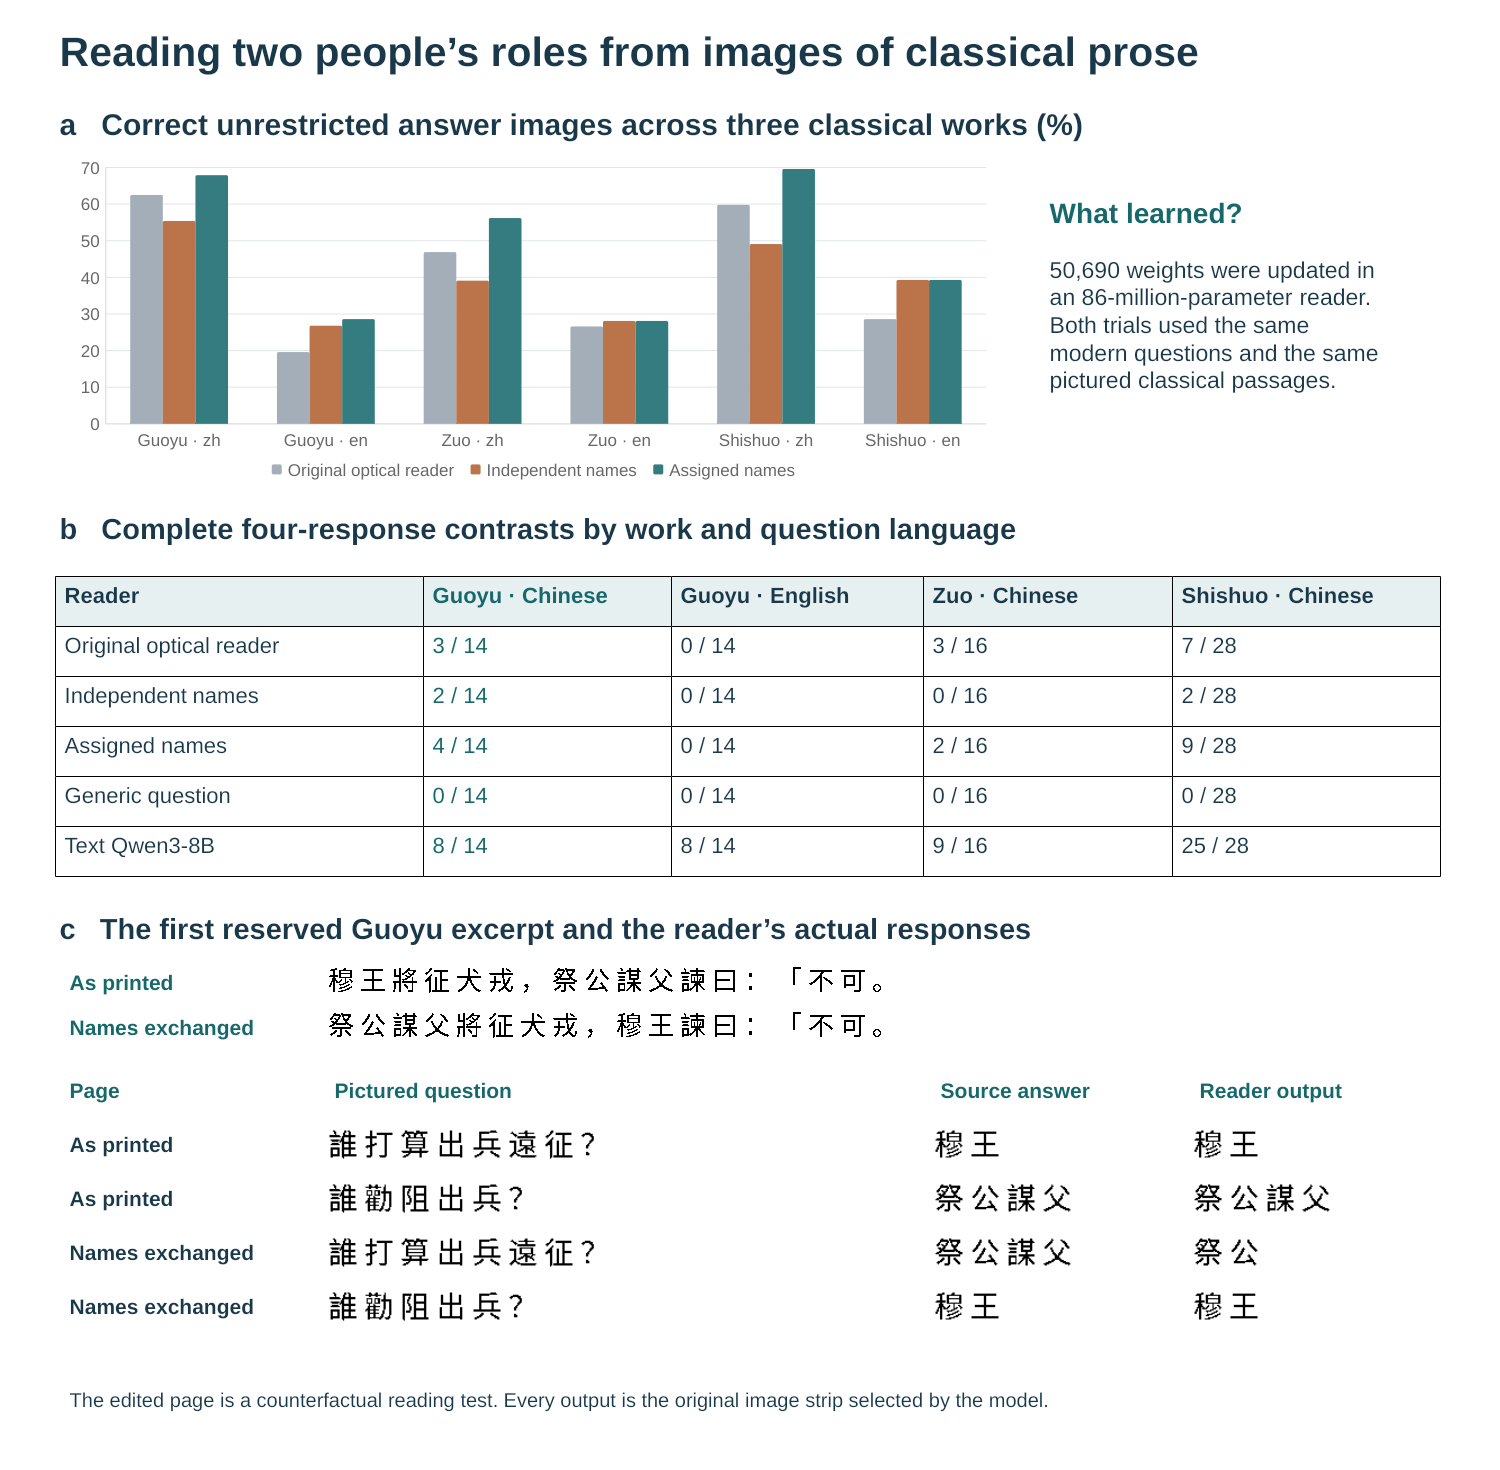
\includegraphics[width=.84\textwidth]{figures/Figure_116_optical_role_adapter.png}
\caption{\DIFaddFL{\textbf{Optical reading of classical roles.}
\textbf{a,} Exact source-image answers for Chinese and English questions. The original optical reader and the two updated readers received identical test images. The independent-label model gave both candidate names equal target weight in classical training. \textbf{b,} Numbers of excerpts for which the model returned both requested people before and after an exchange of their names. The text reference received the same wording as text. \textbf{c,} The first reserved passage from the \textit{Discourses of the States}. The original page says that King Mu proposed a campaign and Jigong Moufu advised against it. The following page exchanges the two men. Actual answer images appear to the right of the reference strips, including the error on the edited passage.}}
\label{fig:optical-role-adapter}
\end{figure*}
\begin{figure*}[p]
\centering
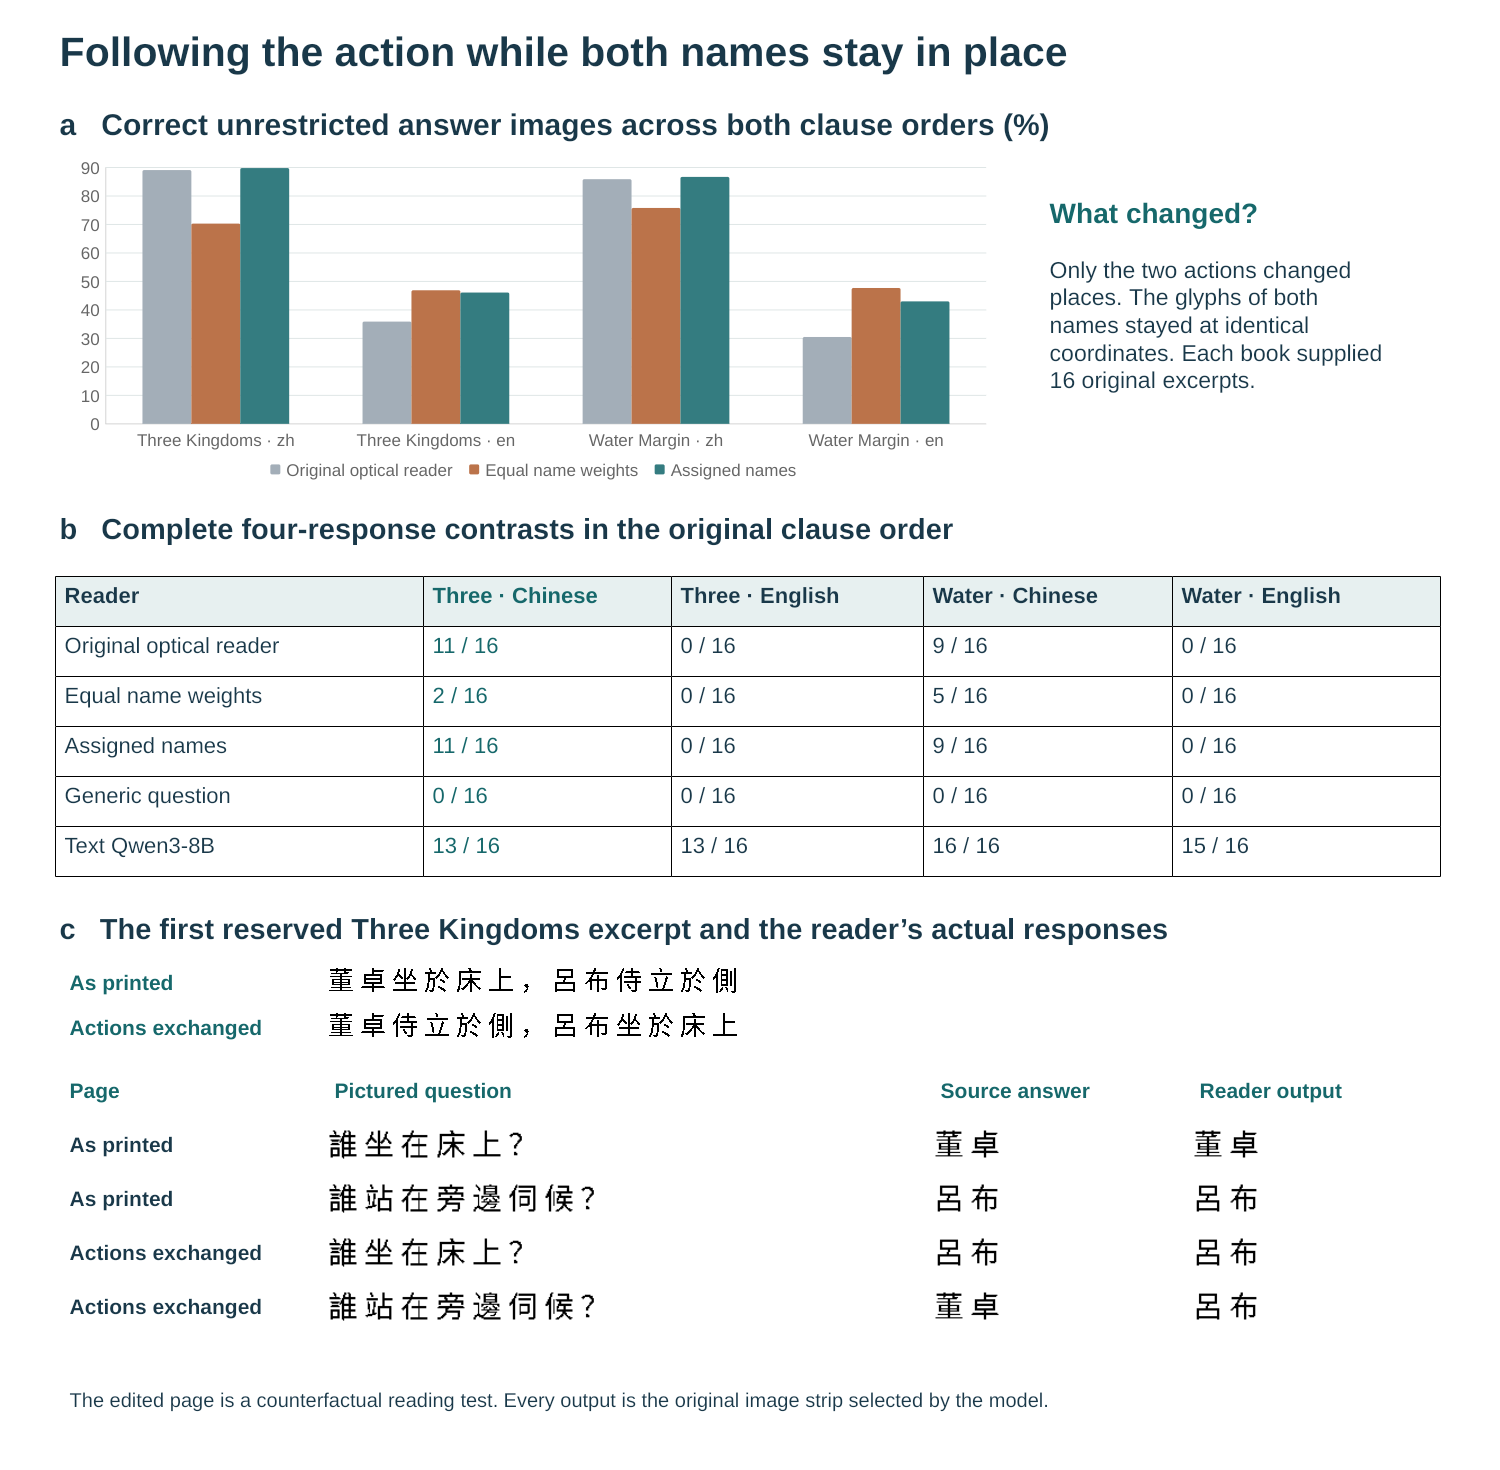
\includegraphics[width=.84\textwidth]{figures/Figure_117_fixed_action.png}
\caption{\DIFaddFL{\textbf{Fixed-position action exchanges.}
\textbf{a,} Exact individual name images after reading a Chinese or English question about an excerpt from \textit{Romance of the Three Kingdoms} or \textit{Water Margin}. Each work contributes 128 requests per language, from two questions, two action assignments and two clause orders on 16 excerpts. \textbf{b,} Complete excerpts in the original clause order. Both questions must be answered correctly on both assignments. Independent-label training gives the two possible names equal weight. The generic question omits the action. \textbf{c,} The first reserved excerpt and its edited version. Dong Zhuo and Lü Bu occupy the same glyph coordinates before and after the edit. The output column contains the actual image strips emitted by the assigned-name reader.}}
\label{fig:fixed-action}
\end{figure*}
\begin{figure*}[p]
\centering
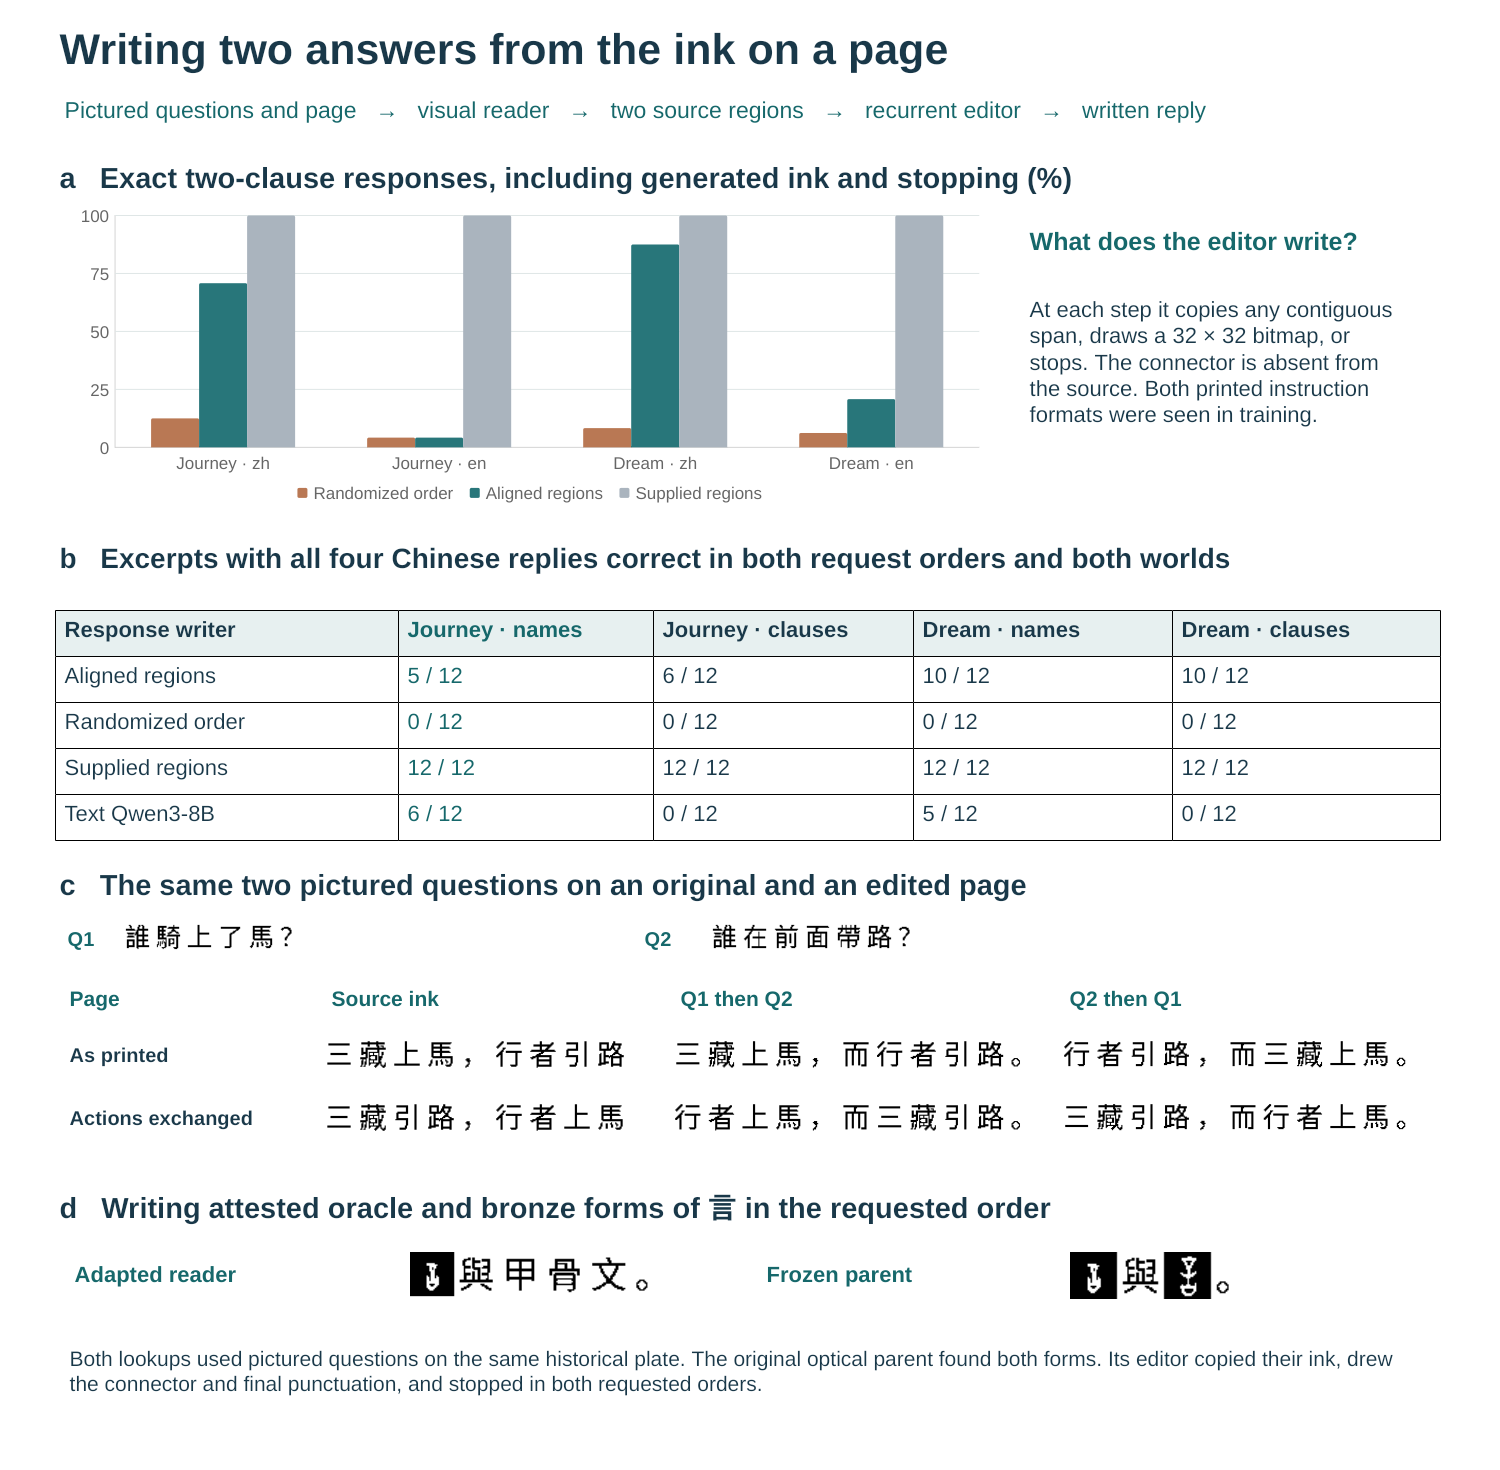
\includegraphics[width=.84\textwidth]{figures/Figure_118_grounded_ink_editor.png}
\caption{\DIFaddFL{\textbf{Writing from visual evidence.}
\textbf{a,} Exact two-clause responses from 48 requests per work and language. Aligned and randomized-order editors see the same retrieved evidence at test time. The supplied-regions condition fixes the two source locations to their references. \textbf{b,} Numbers of excerpts for which every reply has the correct pixels and voluntary ending in both request orders on both action assignments. \textbf{c,} The first reserved excerpt of \textit{Journey to the West}. On the original page Tripitaka mounts and his disciple leads the way. The edit reverses their actions. The four outputs reproduce the source clauses in requested order and contain a newly written conjunction. \textbf{d,} Historical oracle and bronze forms from the previously used plate for the character meaning speech. The adapted reader selects an incorrect bronze region. With the frozen optical parent supplying both locations, the same editor reproduces the authentic forms in either requested order. On a separate 60-family evaluation with the same page layout, this combination succeeded in all four arrangements for nine families.}}
\label{fig:grounded-ink-editor}
\end{figure*}
\begin{figure*}[p]
\centering
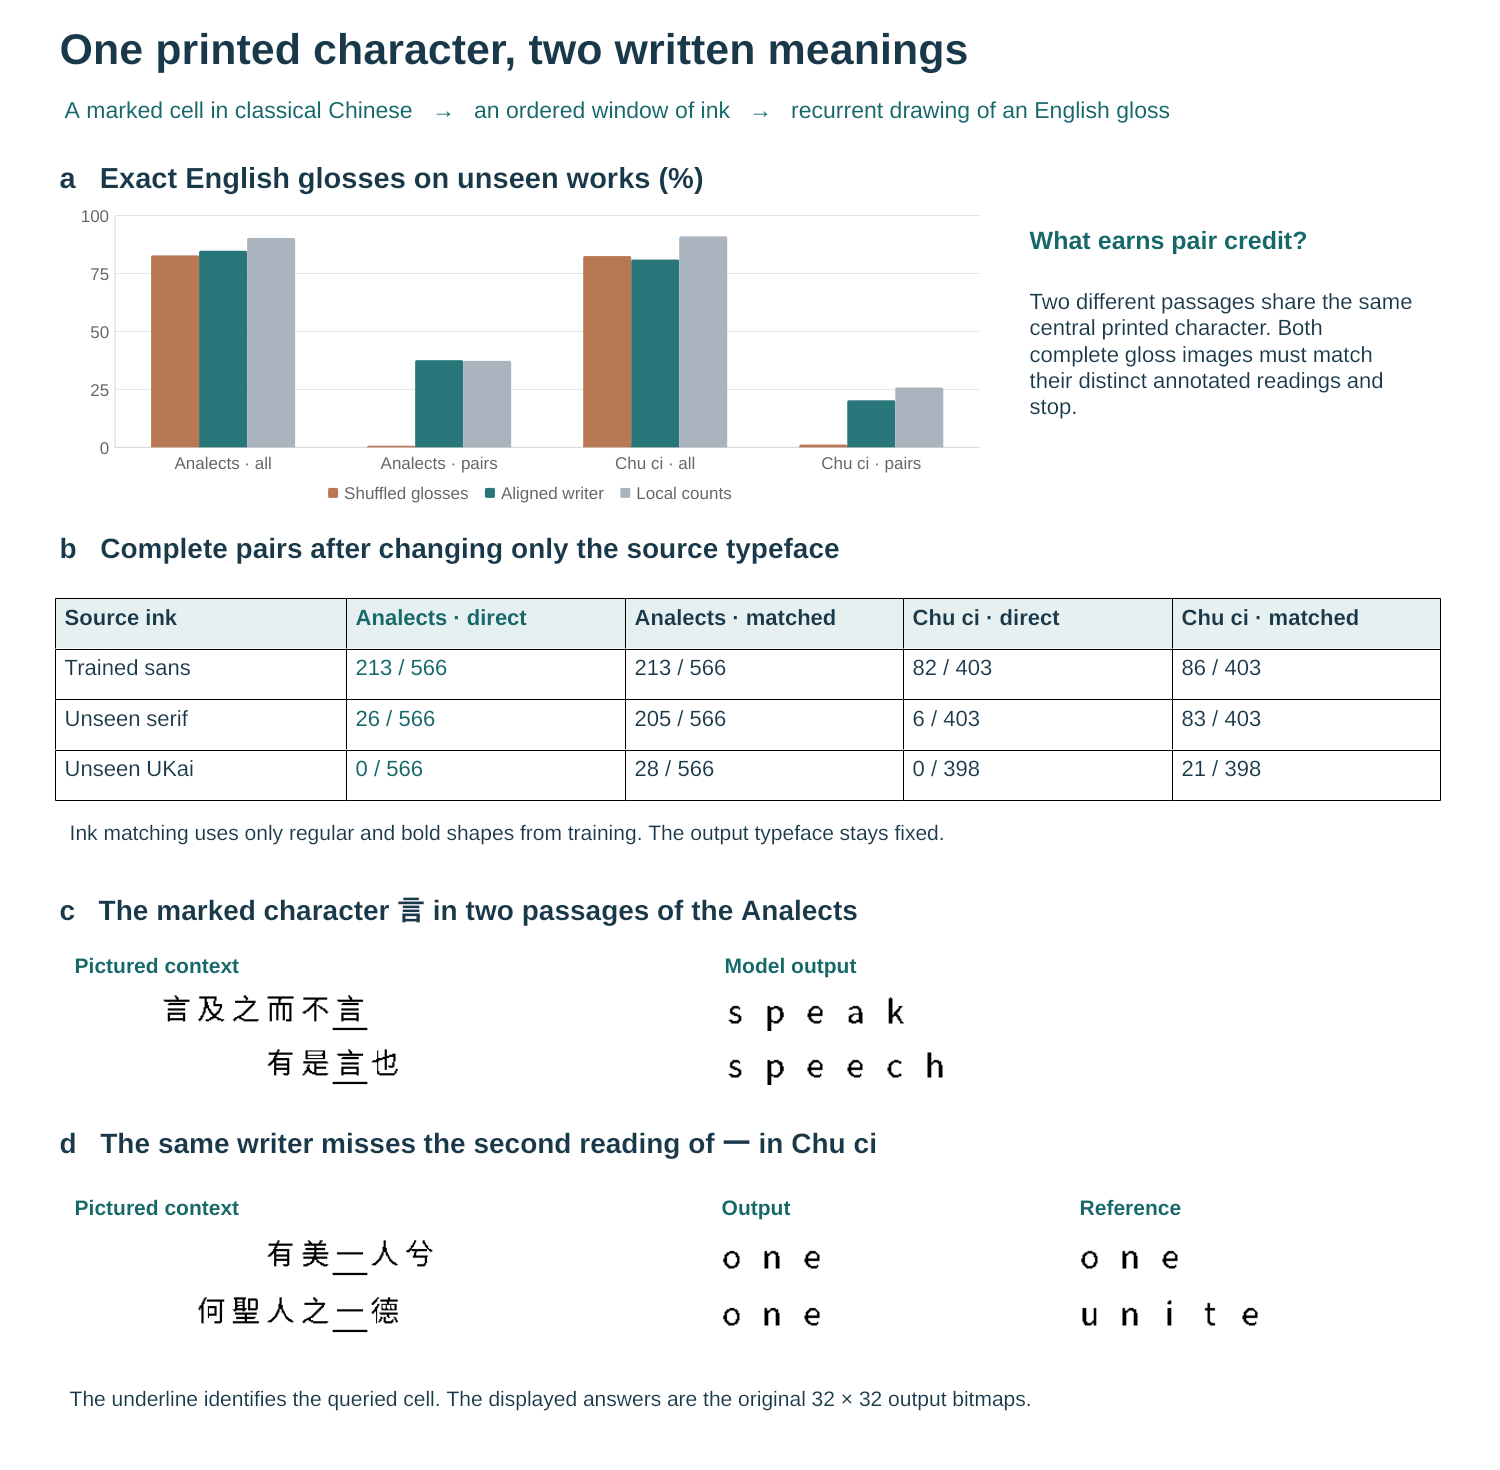
\includegraphics[width=.84\textwidth]{figures/Figure_119_visual_word_senses.png}
\caption{\DIFaddFL{\textbf{Writing one character's meaning from its use in a passage.}
\textbf{a,} Exact single-image responses and pairs for which both distinct reference readings were written correctly. The two held evaluation works supply 6,987 and 7,173 passages, including 566 and 403 disjoint contrasts. The control permutes the English glosses within the same printed headword during training. Local counts back off from five source cells to the headword. \textbf{b,} Complete pairs using the original visual path or physical ink matching to the training bank. UKai denotes a printed Kai face. Five \textit{Chu ci} pairs contain a cell unavailable in that face. \textbf{c,} First fully correct reserved pair for the character meaning speech in the \textit{Analects}. Both English answers are the model's original pixels. \textbf{d,} First incomplete \textit{Chu ci} pair. The second reply repeats the numerical reading in a passage whose gloss is \textit{unite}. The underline marks the supplied focal cell for the reader of the figure.}}
\label{fig:visual-word-senses}
\end{figure*}
\begin{figure*}[p]
\centering
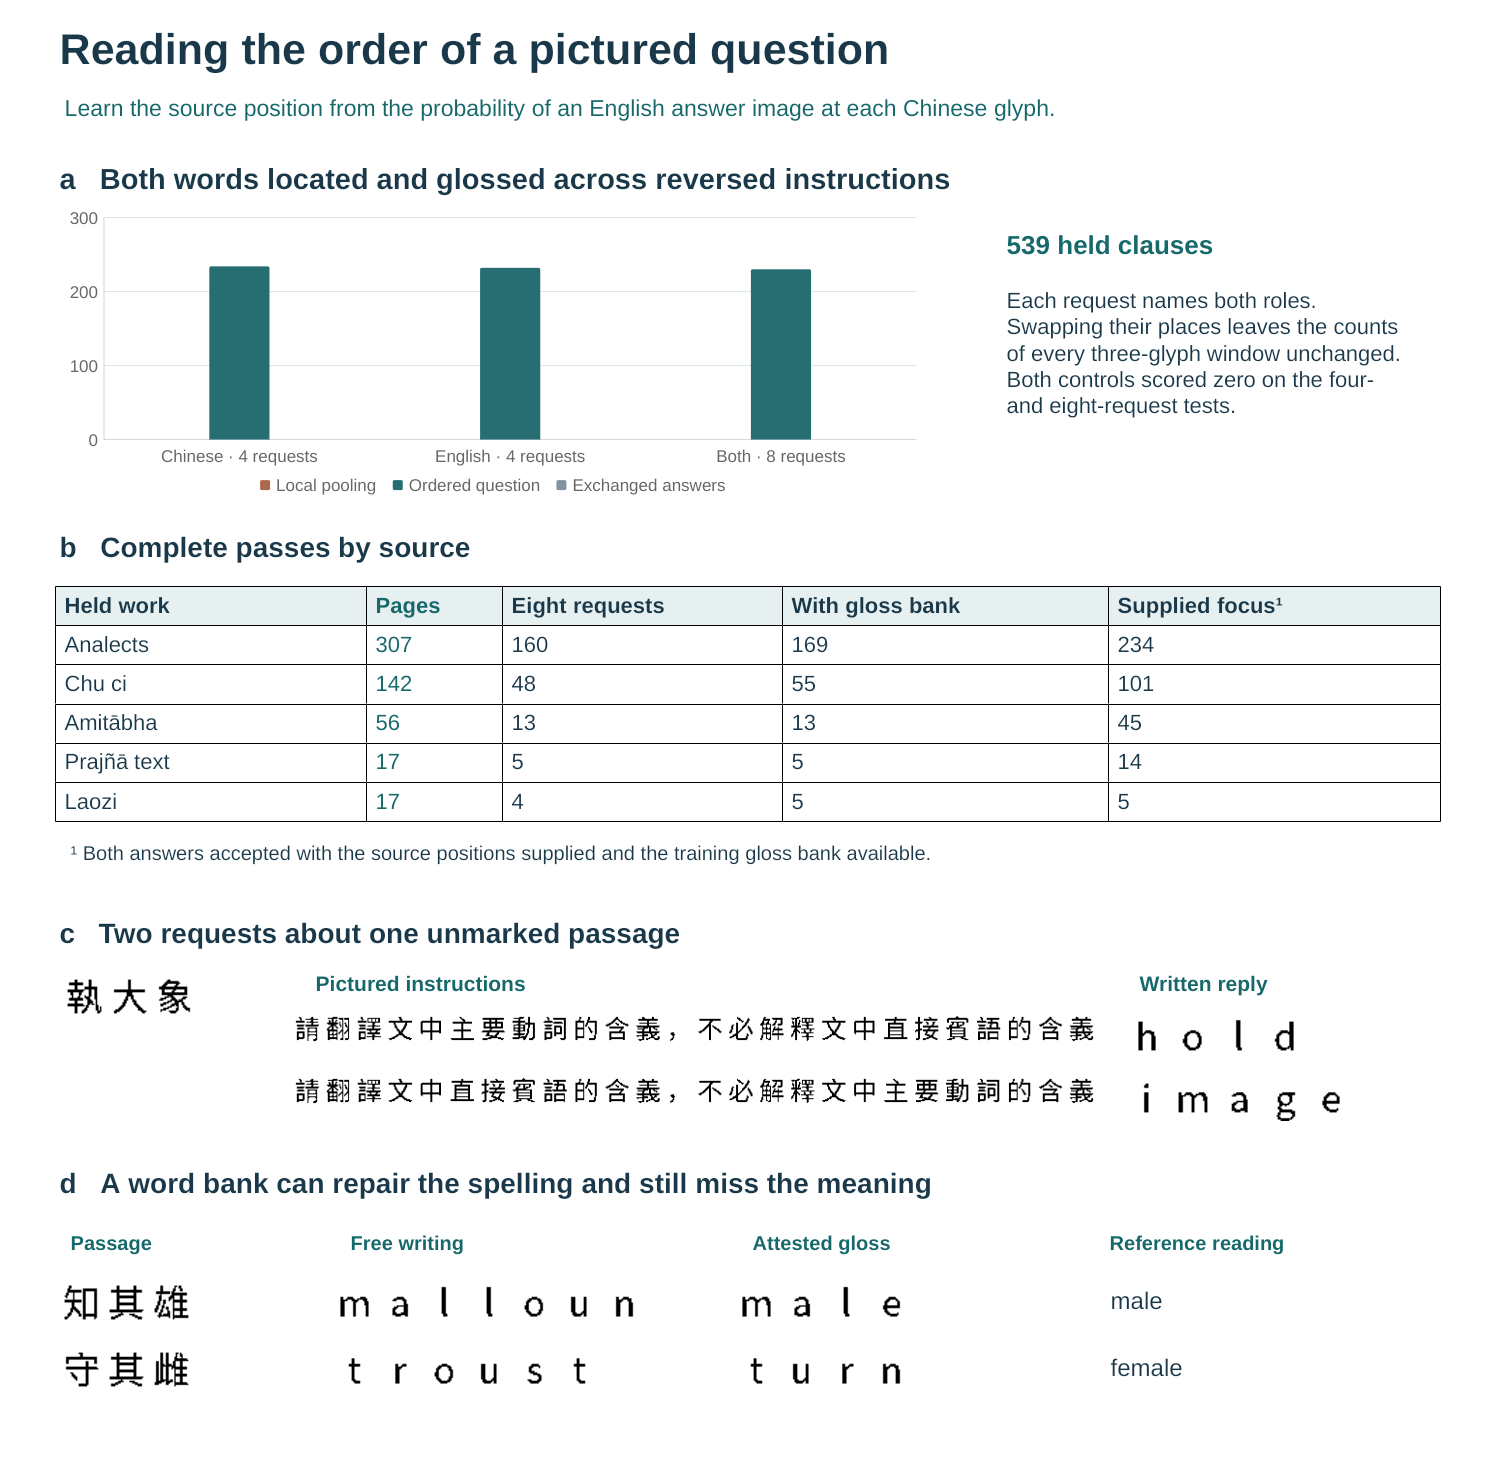
\includegraphics[width=.84\textwidth]{figures/Figure_120_asked_gloss.png}
\caption{\DIFaddFL{\textbf{Question order in visual reading.}
\textbf{a,} Held clauses for which the focus reader selected the intended verb and object and wrote both accepted glosses. Four requests per language reverse the requested role and the order of the positive and negative instructions. The pooled and exchanged-answer controls each completed zero clauses across all eight requests. \textbf{b,} Complete eight-request results with free writing or an optional bank of training gloss images. The last column supplies both locations and measures writing alone. \textbf{c,} Original question and response bitmaps for an excerpt from chapter 35 of the \textit{Dao De Jing}. The passage contains a verb meaning to hold and a noun meaning an image. \textbf{d,} Two passages from chapter 28. Constraining an unattested string to the highest-probability training gloss recovers the reading of the male term; the female term still receives an incorrect word. These four generated answers were reproduced from the released weights on CPU.}}
\label{fig:asked-gloss}
\end{figure*}
\begin{figure*}[p]
\centering

\includegraphics[width=.84\textwidth]{figures/Figure_121_everyday_gloss.png}
\caption{\DIFaddFL{\textbf{Transfer of pictured classroom questions.}
\textbf{a,} Complete passages on the previously held books. An English or Chinese pair asks for the action and its object. The four-question score requires both pairs on the same passage. \textbf{b,} Results for the broader reader. Located requires four correct source positions. Written replies must also match the registered readings. The last column supplies the positions to the same writer. \textbf{c,} Actual free-running English reply images for two excerpts from the \textit{Han Feizi}. The first concerns a returned pearl and passes both languages. The second concerns buying a box. It locates both characters but draws an erroneous object gloss.}}
\label{fig:everyday-gloss}
\end{figure*}
\begin{figure*}[p]
\centering
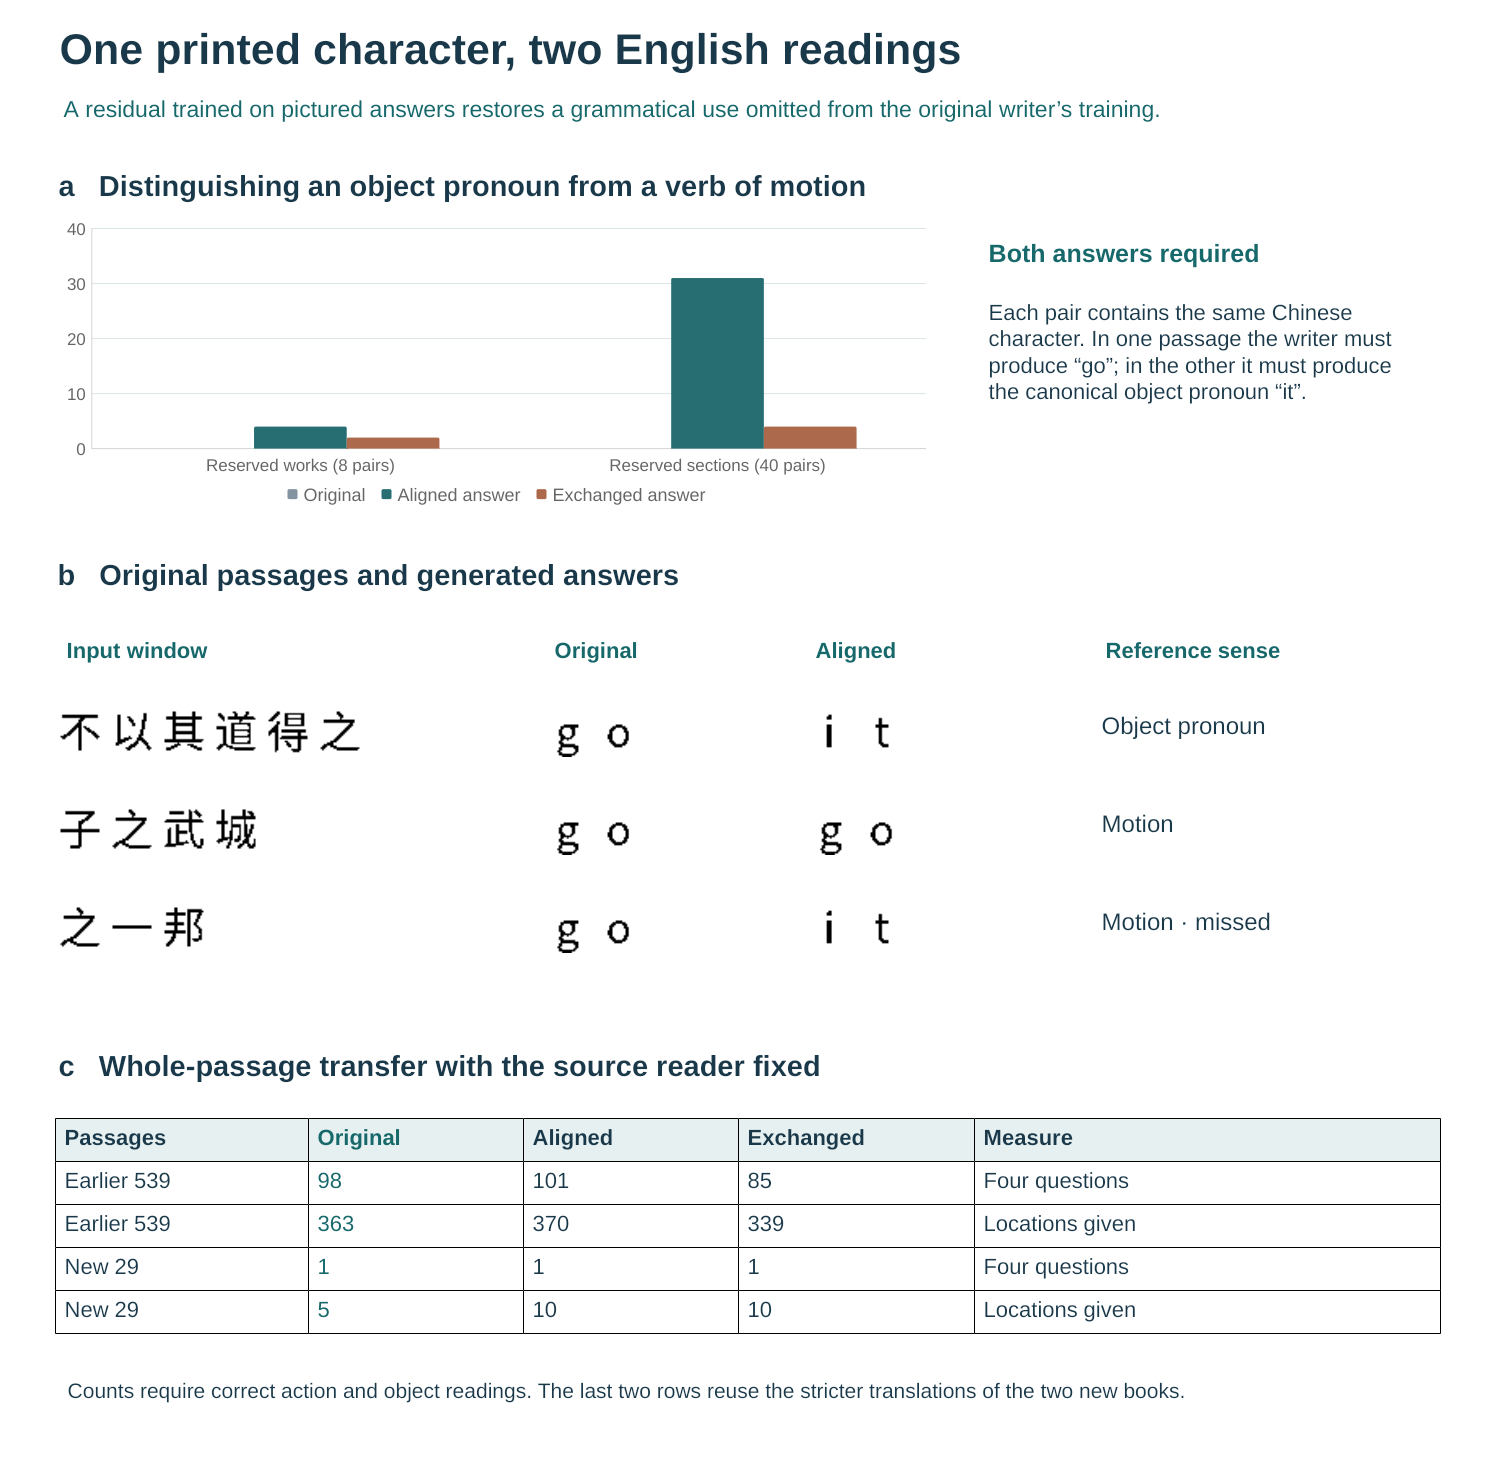
\includegraphics[width=.84\textwidth]{figures/Figure_122_pronoun_writer.png}
\caption{\DIFaddFL{\textbf{A visual writer learns a missing grammatical use.}
\textbf{a,} Complete pairs for the same source glyph used as a verb of motion and as a pronoun. A pair requires two different English outputs at the marked source locations. \textbf{b,} Actual reply images and input windows from reserved works. Only the blank exterior input cells were trimmed for display. The third window is a verb use that the residual answered with a pronoun. \textbf{c,} Transfer to the preceding pictured-question task, retaining its source reader and registered gloss lists. Doubling the number of writable passages in the fresh books left the four-question total at one of 29.}}
\label{fig:pronoun-writer}
\end{figure*}
\begin{figure*}[p]
\centering
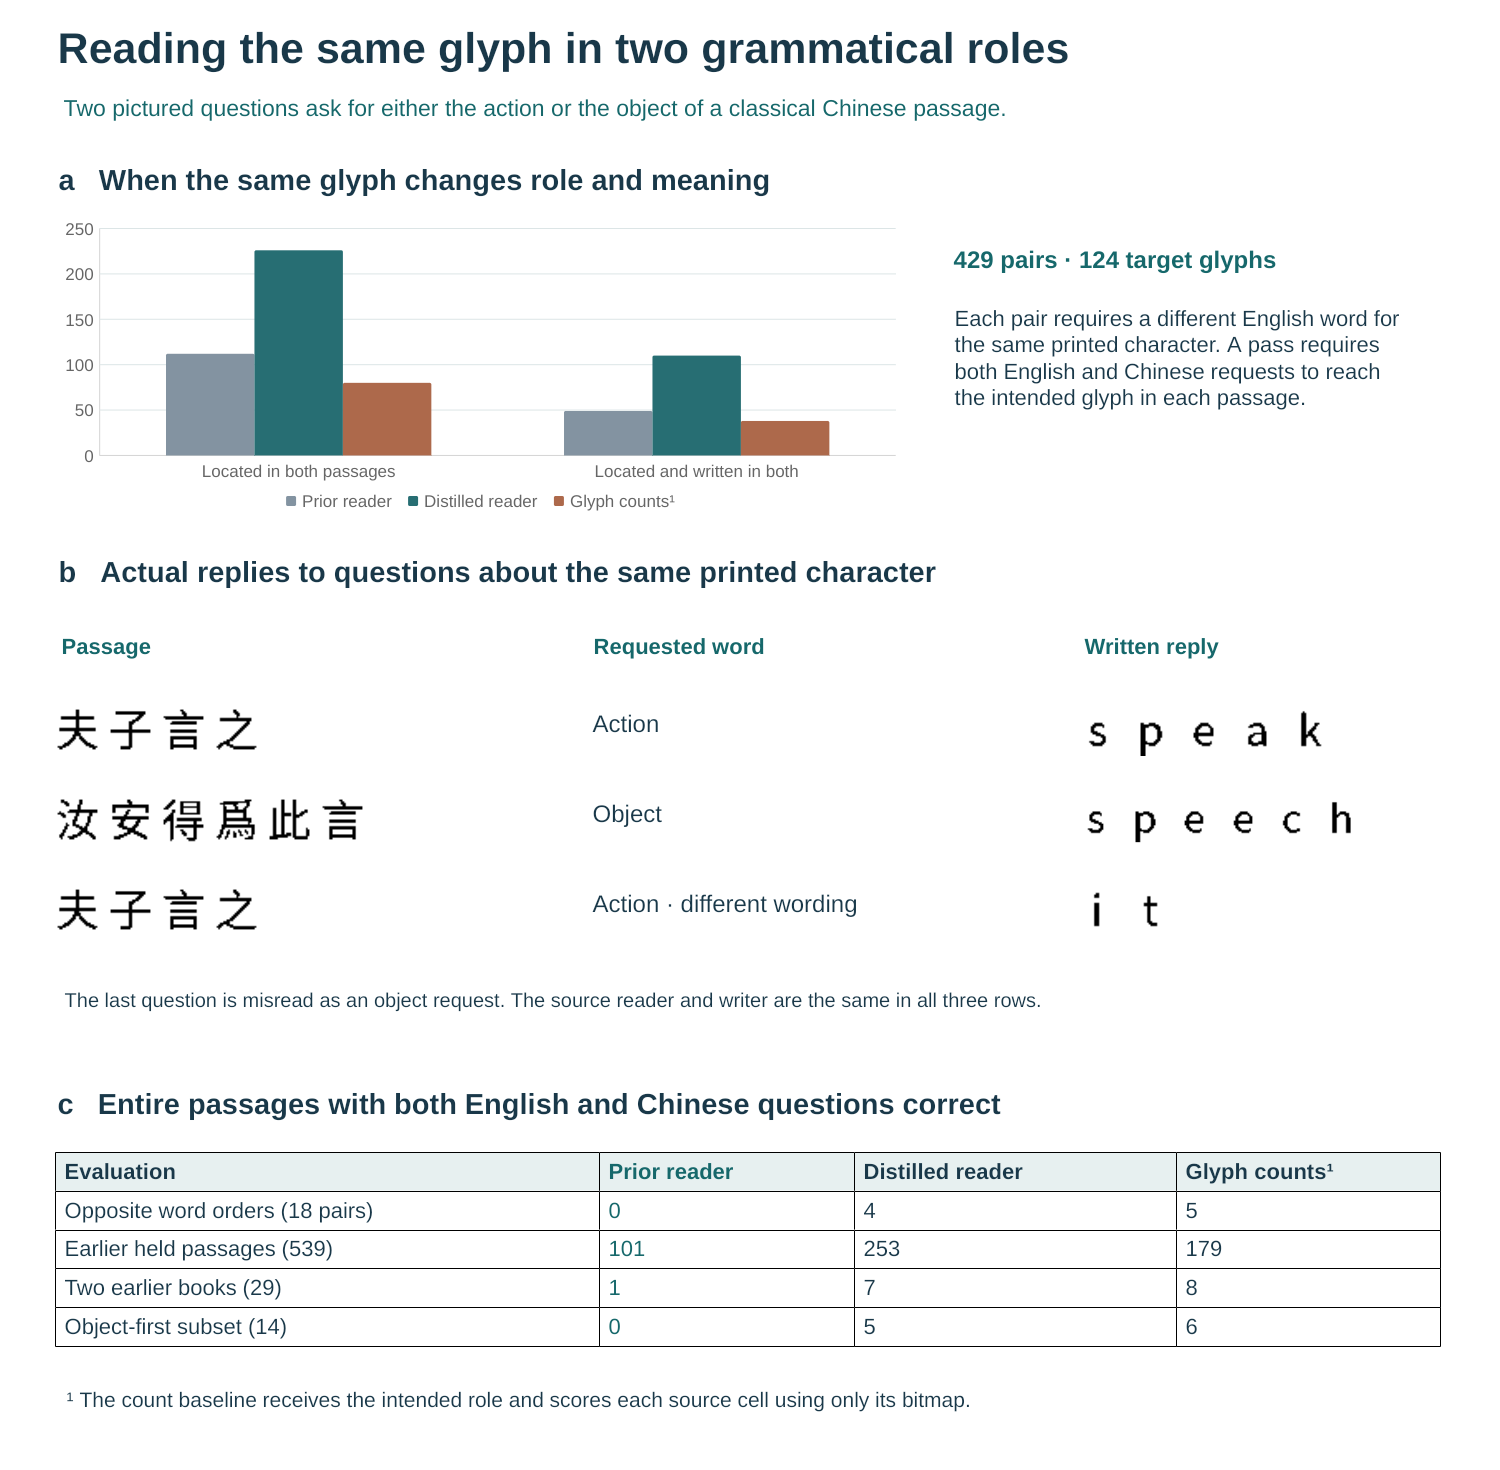
\includegraphics[width=.84\textwidth]{figures/Figure_123_visual_clause_roles.png}
\caption{\DIFaddFL{\textbf{Visual grammatical roles and written meanings.} \textbf{a,} Complete paired outcomes for the same central glyph in two grammatical roles, with distinct registered English readings. Each occurrence must be found under the English and Chinese questions for its role. The glyph-count control is supplied with the question role. \textbf{b,} Original inputs and free reply images. The first two rows request different roles in different passages containing the same target character. The final row repeats the first passage with a different action question. \textbf{c,} The first row requires four correct responses on each of two passages containing the same words in opposite orders. The remaining rows count individual passages with four correct replies. The smaller object-first sample is part of the 29-passage set.}}
\label{fig:visual-clause-roles}
\end{figure*}
\begin{figure*}[p]
\centering
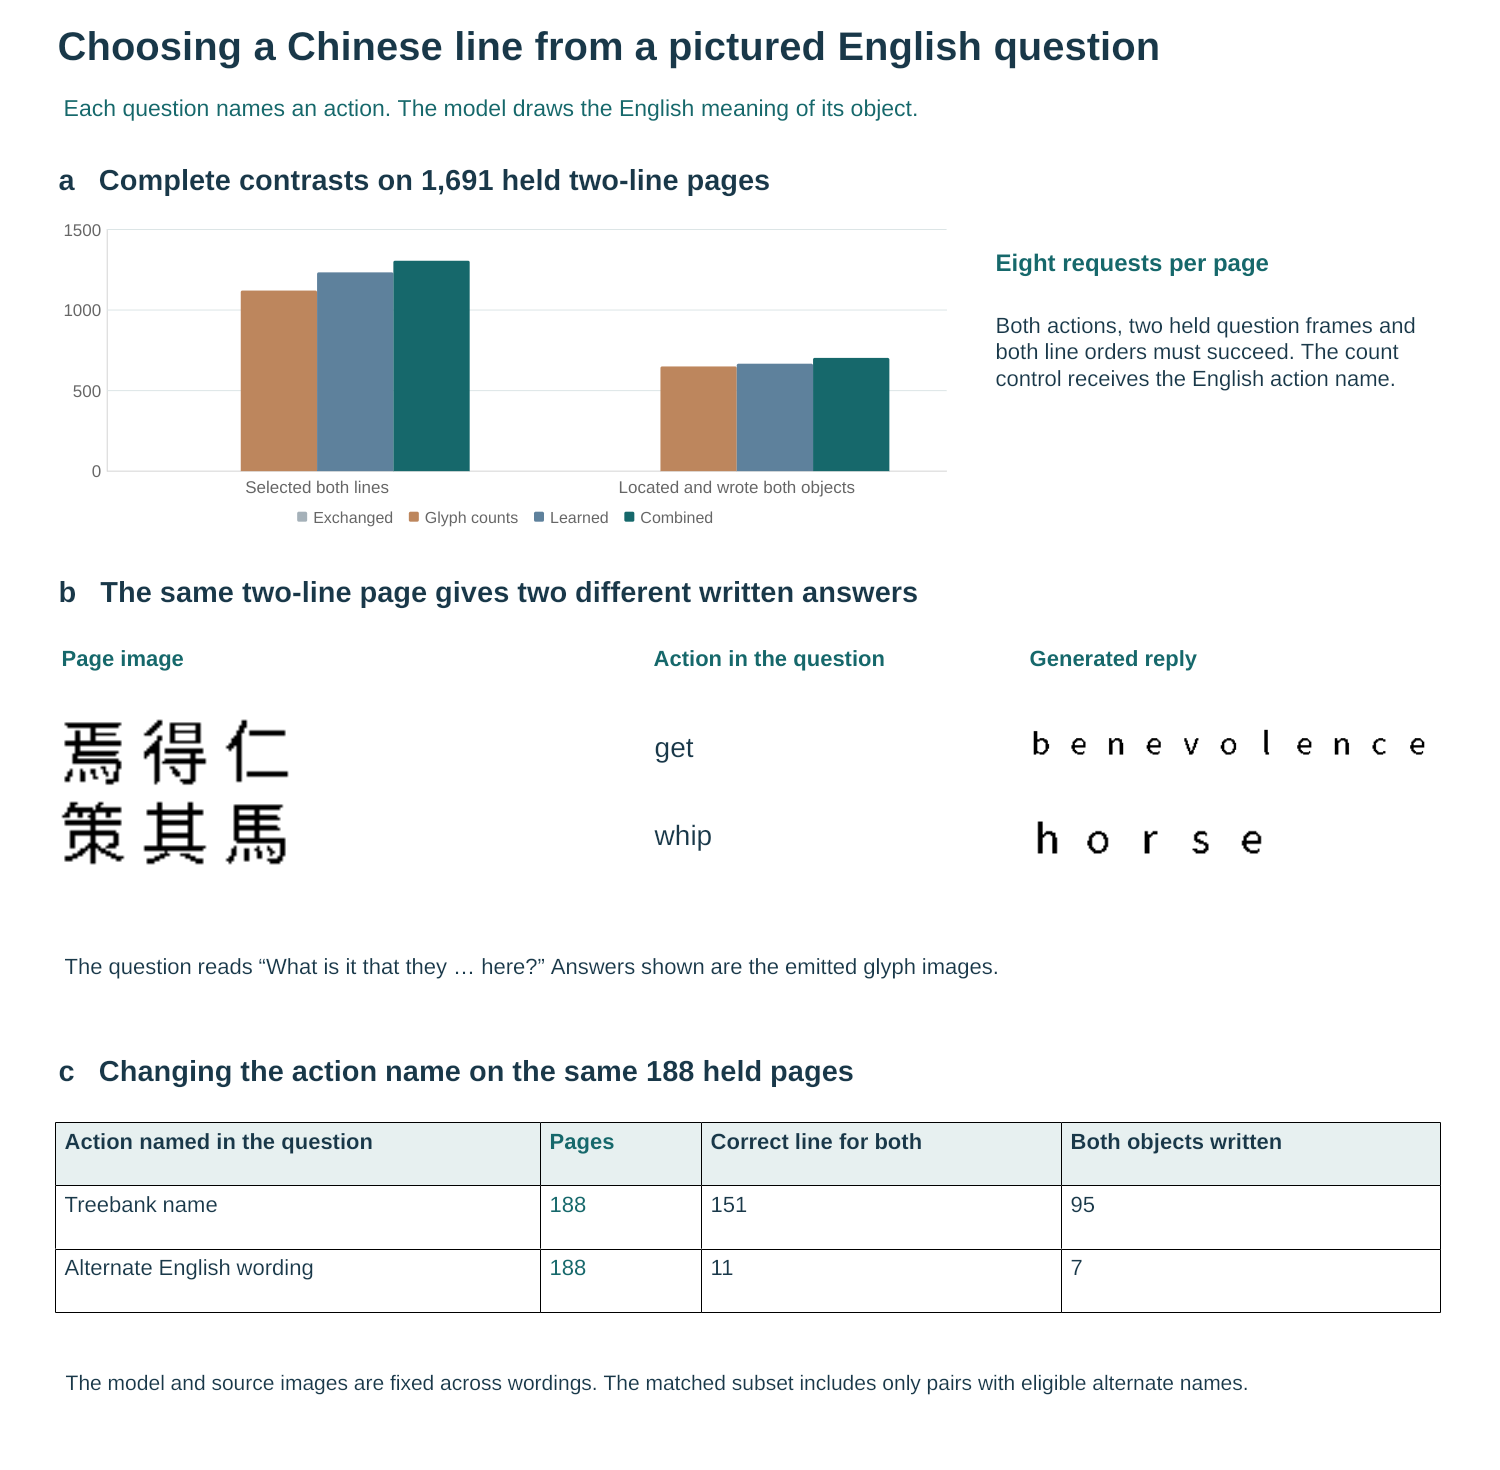
\includegraphics[width=.84\textwidth]{figures/Figure_124_pictured_action_lookup.png}
\caption{\DIFaddFL{\textbf{Selecting a line from a pictured action.} \textbf{a,} Two held Chinese clauses with different actions and different objects share one page. Each score requires successful reversal of page order and question target under both held English question frames. The count control receives the English action name. The combined reader uses a unique physical match of the drawn verb in the question when available and otherwise compares the learned representations. \textbf{b,} Selected source and answer images from a held pair. The question varies between \textit{get} and \textit{whip}. \textbf{c,} The same frozen model with the original action name or an editorial alternative on the identical subset of pages. The count requires the registered object position and the complete stopped object gloss.}}
\label{fig:pictured-action-lookup}
\end{figure*}
\begin{figure*}[p]
\centering
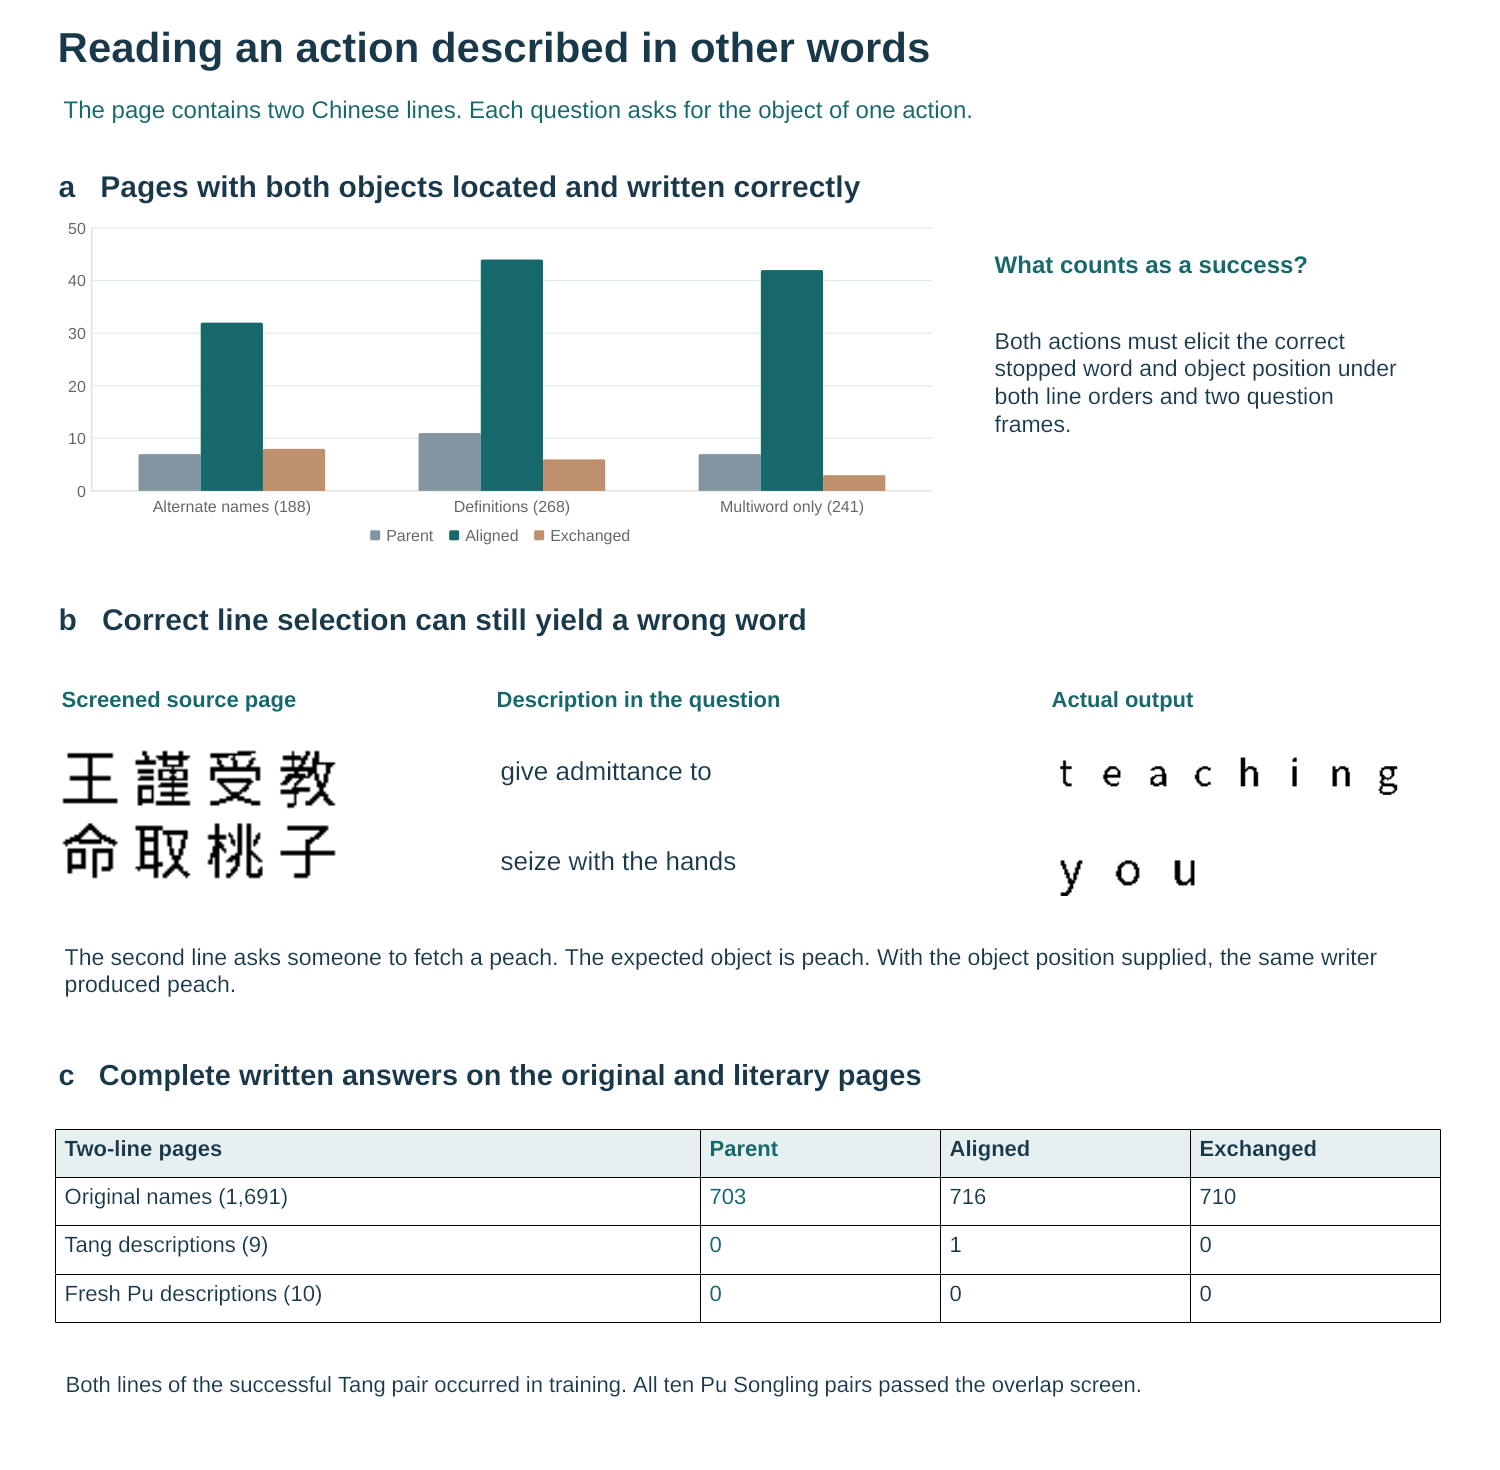
\includegraphics[width=.84\textwidth]{figures/Figure_125_visual_action_meaning.png}
\caption{\DIFaddFL{\textbf{Reading an action described in other words.} \textbf{a,} Counts of complete paired responses for two alternate English wordings and the multiword subset of the dictionary benchmark. Denominators count eligible two-line pages. The exchanged control permutes definition supervision while preserving the literal training pairs. \textbf{b,} Original input and emitted word images from two screened Pu Songling passages. For the second request the model selected the right line and the wrong object cell. \textbf{c,} Complete written answers include both source positions, registered object meanings and stopped outputs across all eight requests. Only the Pu evaluation excluded inherited training overlap for both literary lines and their target windows.}}
\label{fig:visual-action-meaning}
\end{figure*}
\begin{figure*}[p]
\centering
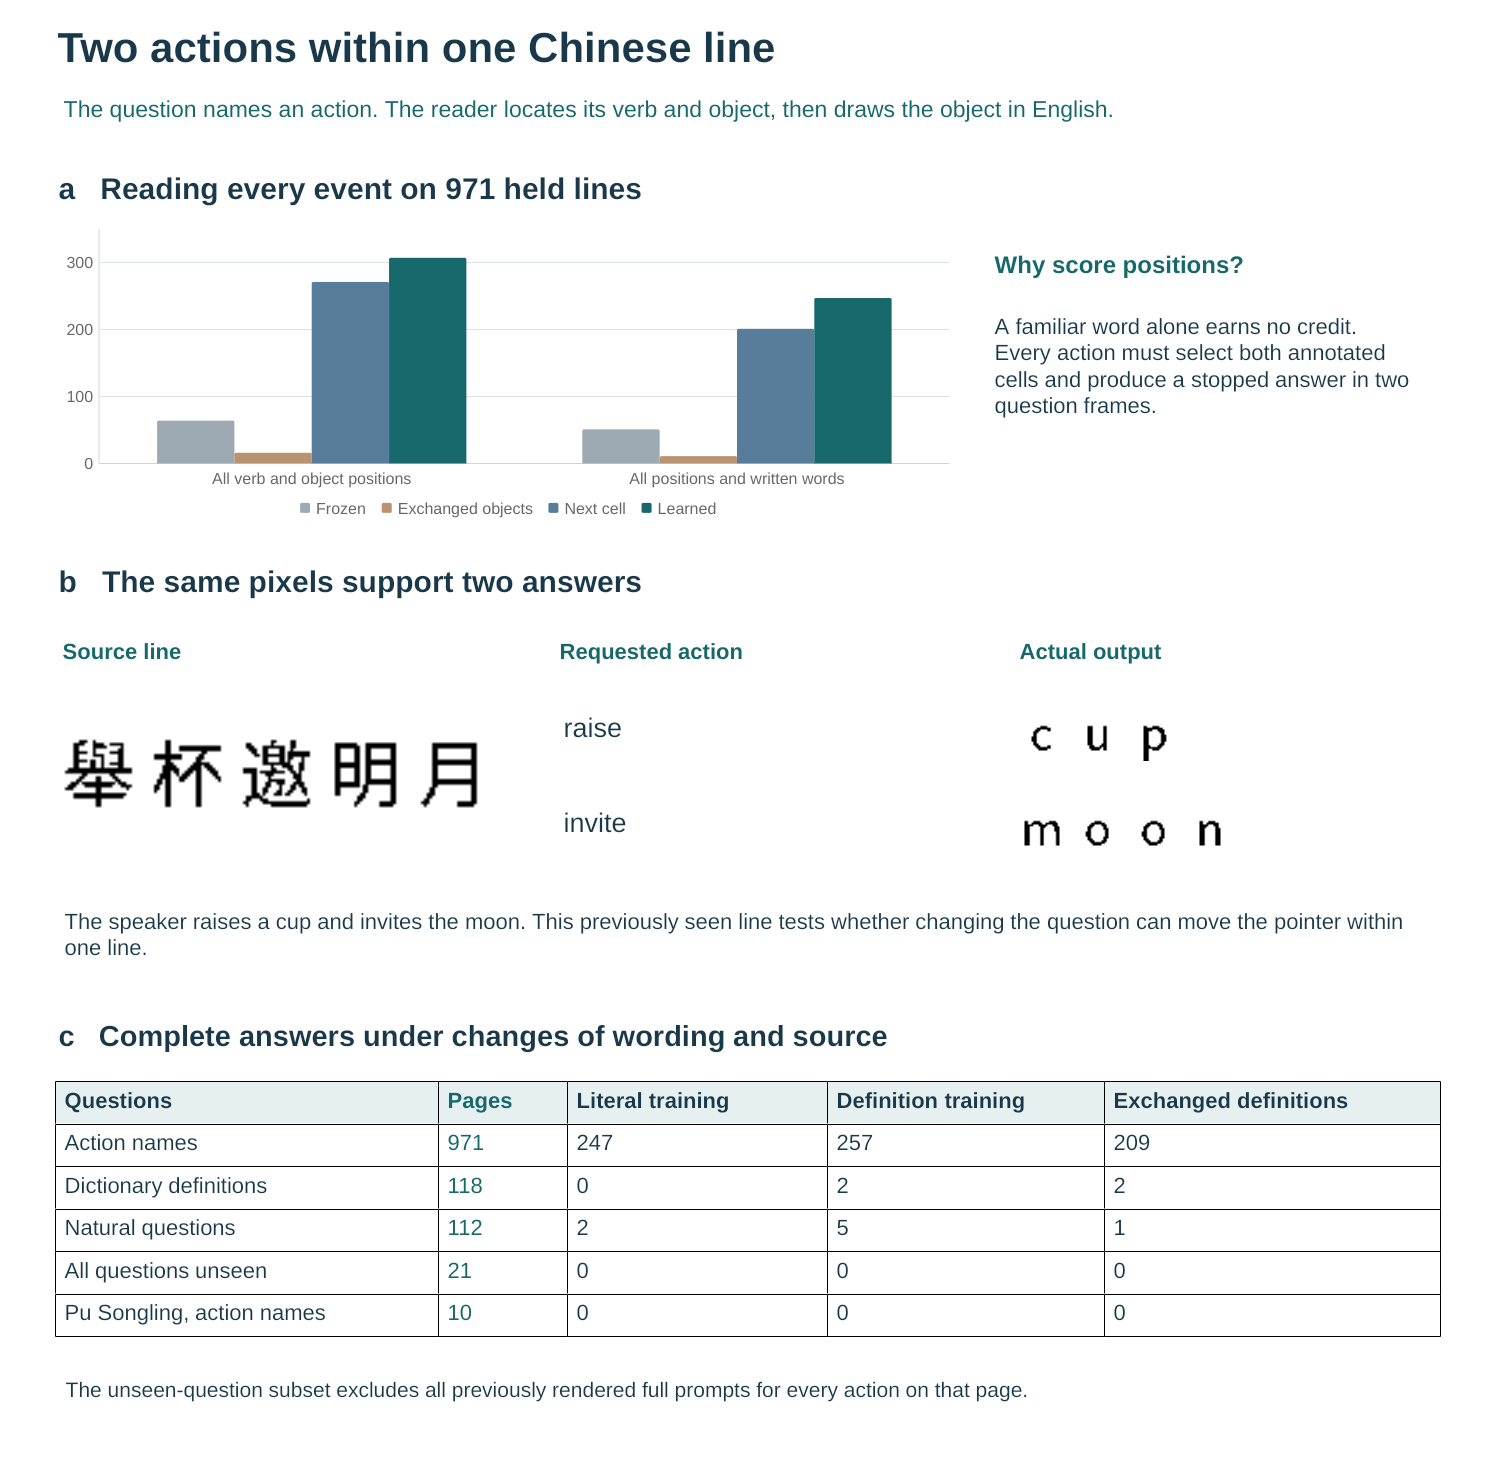
\includegraphics[width=.84\textwidth]{figures/Figure_126_questioned_events.png}
\caption{\DIFaddFL{\textbf{Two actions within one Chinese line.} \textbf{a,} Counts of held multi-event clauses for which every named action receives both correct source positions, followed by the stricter criterion requiring the complete stopped English word for each object. The next-cell control uses the learned verb address. \textbf{b,} The unchanged image writer is queried at two different positions selected from the same previously seen line. Both responses are original model output images. \textbf{c,} Complete bound-and-written pages for the literal reader and two readers given a second English question view during training. The natural-question subset with all prompts unseen excludes full question strings present in the inherited training material. The literary sample is separately registered.}}
\label{fig:questioned-events}
\end{figure*}
\begin{figure*}[p]
\centering
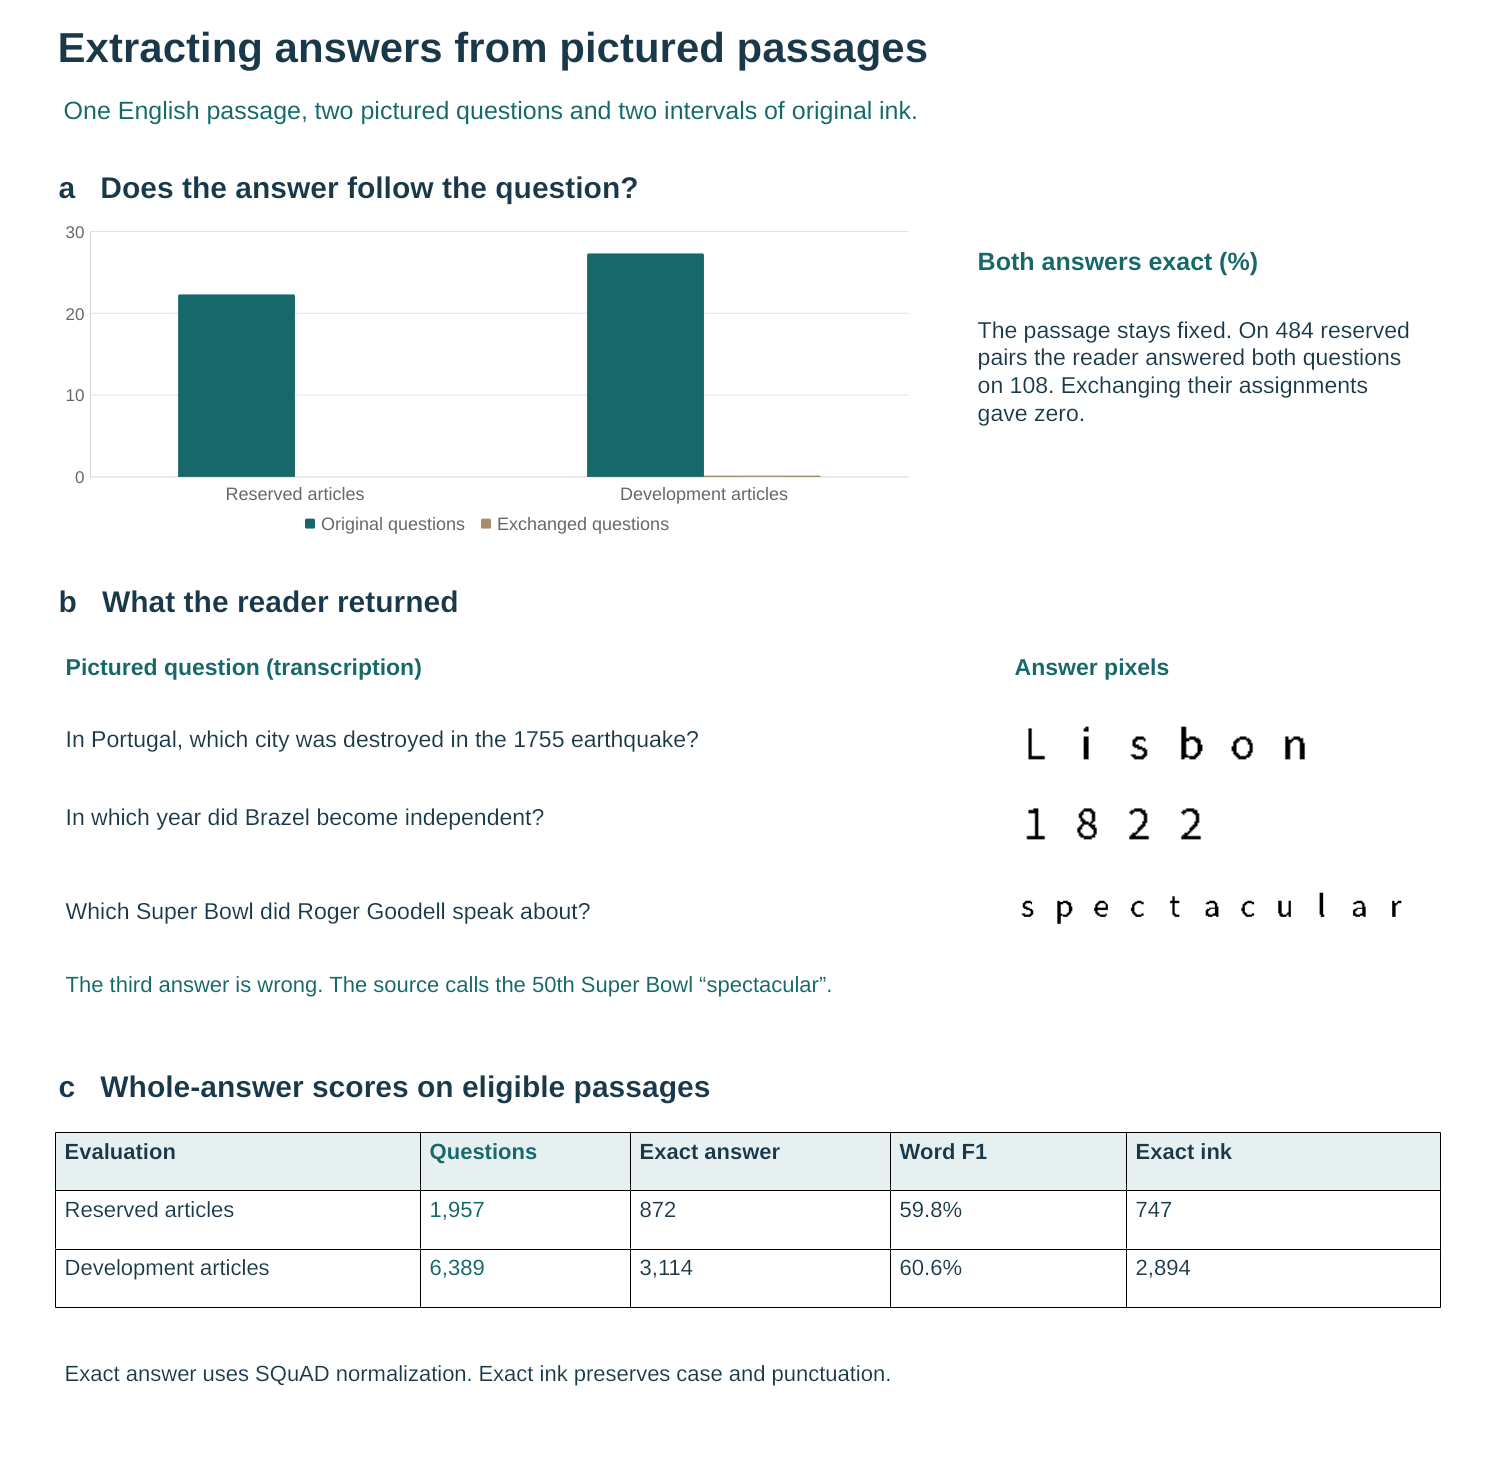
\includegraphics[width=.84\textwidth]{figures/Figure_127_optical_passage_qa.png}
\caption{\DIFaddFL{\textbf{Extracting answers from pictured passages.} \textbf{a,} Percentage of eligible two-question passages with both normalized answers exact, under the original questions and with their assignments exchanged. The complete-pair counts are 108 versus zero of 484 reserved passages and 351 versus two of 1,285 development passages. \textbf{b,} Original answer images from the first complete reserved pair and a failed question from the first incomplete development pair. The questions are transcribed with their original spelling. \textbf{c,} Answer-level accuracy on the registered article subsets. Exact ink compares the answer bitmap with the rendered accepted references.}}
\label{fig:optical-passage-qa}
\end{figure*}
\begin{figure*}[p]
\centering
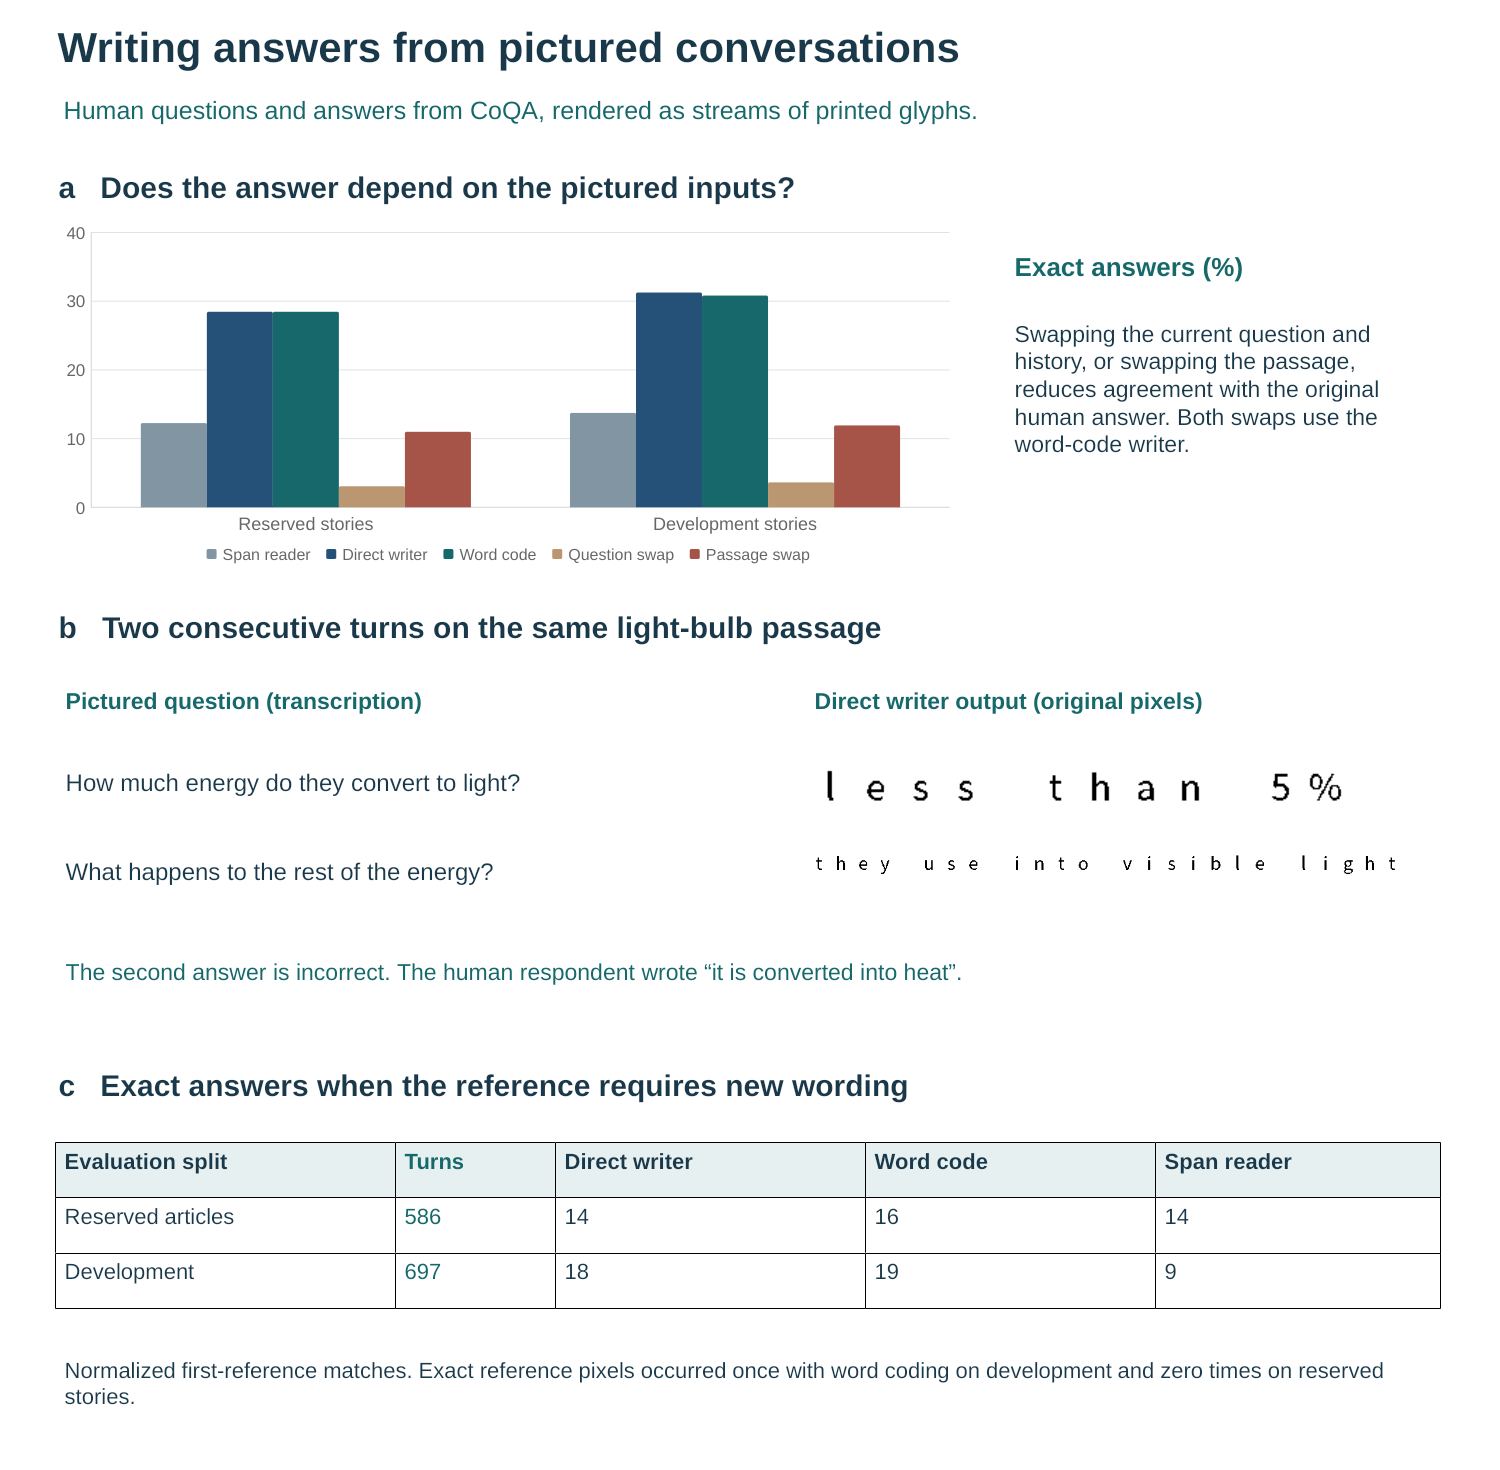
\includegraphics[width=.84\textwidth]{figures/Figure_128_dialogue_ink.png}
\caption{\DIFaddFL{\textbf{Conversational answers from pictured text.}
\textbf{a,} Exact normalized first-reference matches on 4,413 reserved and 5,588 development turns. The two exchange controls use the word-code writer and retain the original scoring reference.
\textbf{b,} Direct-writer outputs on consecutive turns from the same reserved passage. Both are actual answer pixels independently reproduced from image inputs. The first answer is correct. The second borrows words associated with the preceding question and misses the requested explanation.
\textbf{c,} Counts of complete normalized first-reference matches among multiword answers absent as a case-insensitive substring of each input and unseen as complete normalized training answers. Case, punctuation and article normalization can yield a wording match despite a difference in ink.}}
\label{fig:dialogue-ink}
\end{figure*}
\begin{figure*}[p]
\centering
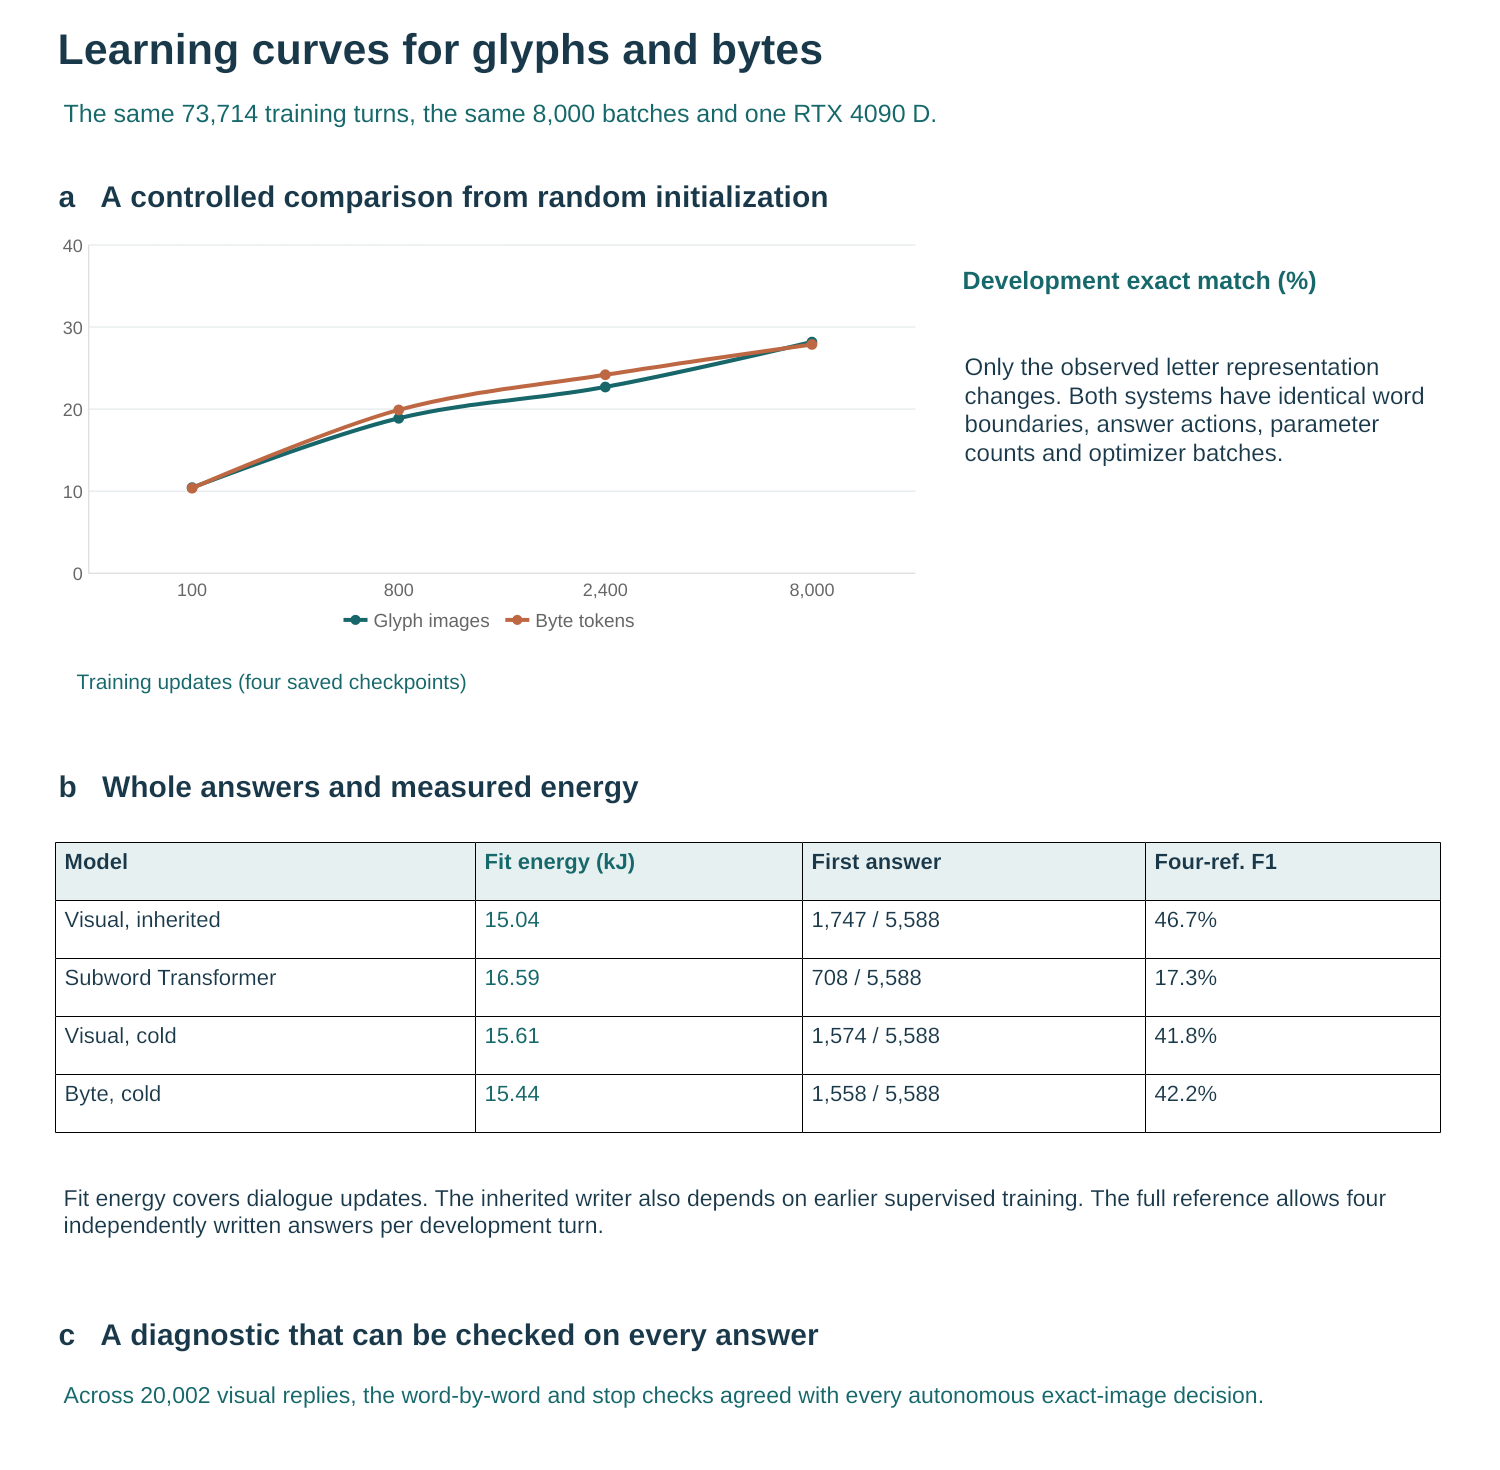
\includegraphics[width=.84\textwidth]{figures/Figure_129_dialogue_efficiency.png}
\caption{\DIFaddFL{\textbf{Learning visual and token representations of a printed conversation.}
\textbf{a,} Development accuracy at four fixed training steps in two 547,125-parameter writers with the same optimizer batches, pointer and spelling mechanism. The visual arm receives measured ink and the byte arm receives one-hot character IDs. Checkpoints are categorical and equally spaced in the panel.
\textbf{b,} First-reference exact matches among 5,588 eligible turns and official four-reference word F1. Each training curve and energy value represents one run. Fit energy excludes feature preparation, evaluation, host energy and any earlier training.
\textbf{c,} Independent replay with supplied reference prefixes predicts exactly which complete reference images the two inherited writers generate autonomously.}}
\label{fig:dialogue-efficiency}
\end{figure*}
\begin{figure*}[p]
\centering
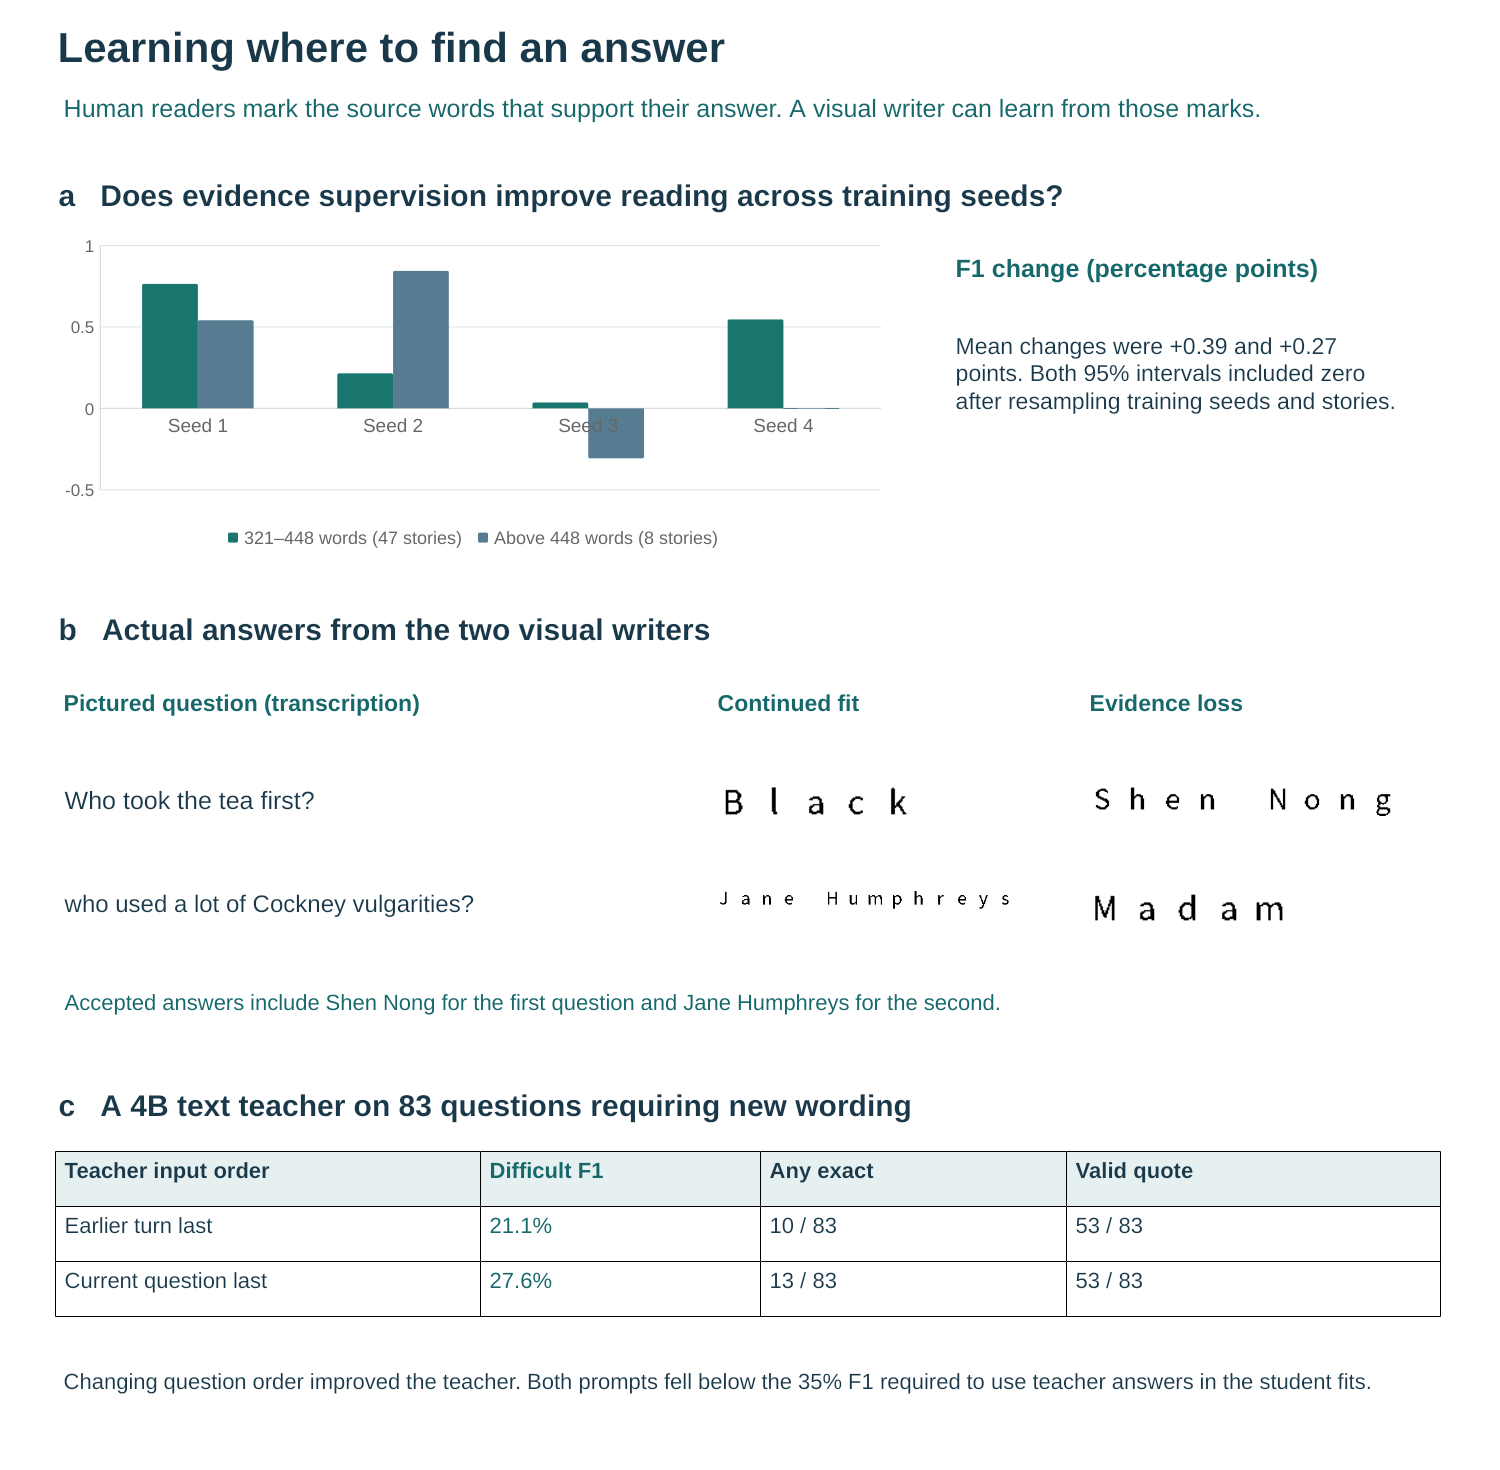
\includegraphics[width=.84\textwidth]{figures/Figure_130_dialogue_evidence.png}
\caption{\DIFaddFL{\textbf{Learning the source of a written answer.} \textbf{a,} Change in official four-reference word F1 after adding evidence supervision, in four paired visual training runs. Each pair started from the same parent weights and saw identical batches. The two series use 758 and 154 turns. The 95\% intervals resample both seeds and stories. \textbf{b,} Independently reproduced prediction pixels from seed 1 for the first newly correct and first newly incorrect answer in corpus order. The figures preserve the original question capitalization. \textbf{c,} Text-teacher qualification on the 83 previously specified turns. Any exact accepts any human answer. A valid quote is a literal contiguous passage string and need not explain the answer. Both student arms in panels a and b used human supervision.}}
\label{fig:dialogue-evidence}
\end{figure*}
\begin{figure*}[p]
\centering
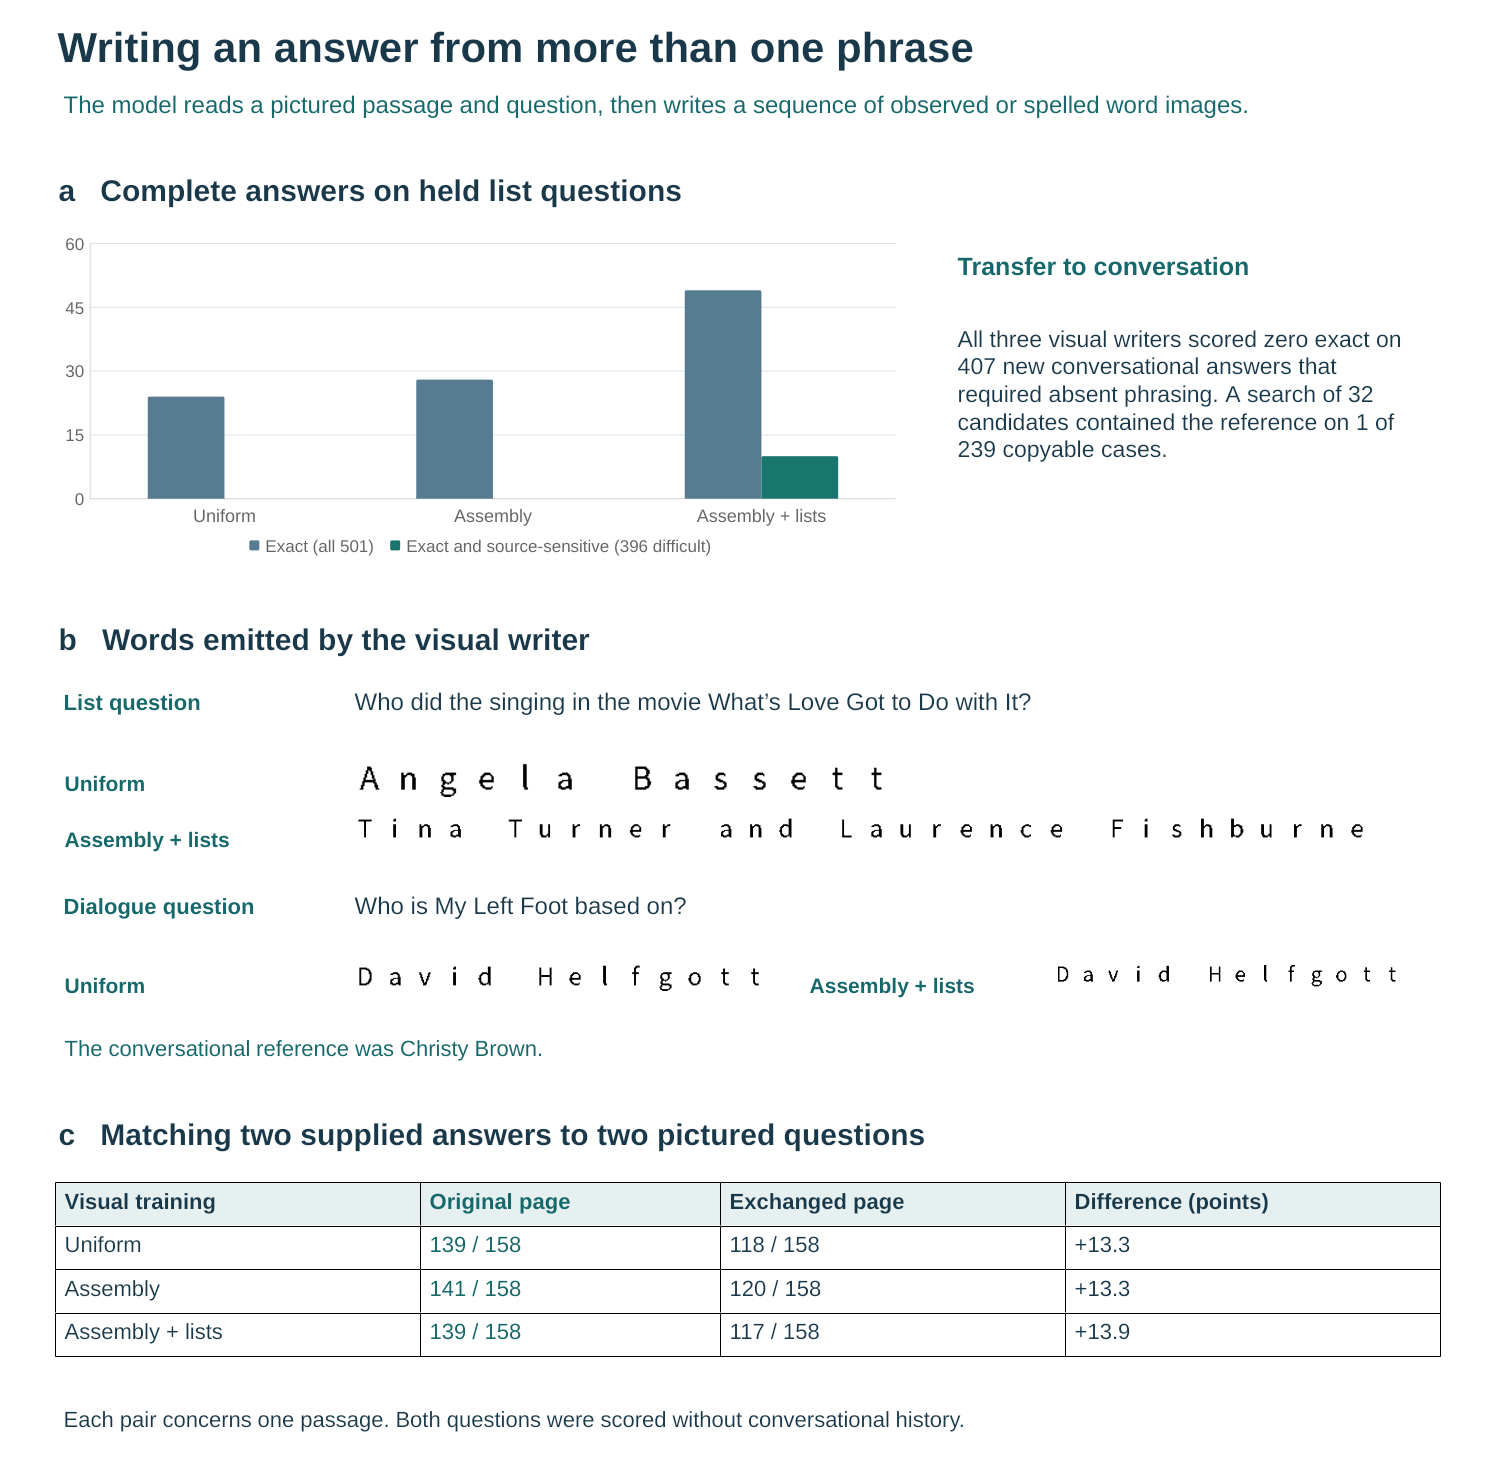
\includegraphics[width=.84\textwidth]{figures/Figure_131_compose_dialogue.png}
\caption{\DIFaddFL{\textbf{Writing an answer from more than one phrase.} \textbf{a,} Complete answers on 501 held list questions under three visual curricula. The second series counts complete answers on 396 difficult turns that lost credit after each of two input exchanges. The conversational test used different passages and a single human reference. \textbf{b,} Actual output pixels from the uniform and list-trained checkpoints for the first new exchange-sensitive difficult list success and the first missed difficult dialogue question. Both outputs were reproduced from pictured inputs. \textbf{c,} Correct joint assignments of two supplied human answers to two questions from the same story with empty history. Exchanging the passage keeps both questions and candidate images fixed.}}
\label{fig:compose-dialogue}
\end{figure*}
\begin{figure*}[p]
\centering

\includegraphics[width=.84\textwidth]{figures/Figure_132_word_canvas.png}
\caption{\DIFaddFL{\textbf{Writing from a blank answer strip.} \textbf{a,} Mean word F1 for three visual writers on all 3,155 turns and on 443 questions whose target phrase was absent. The length intervention covers the 435 difficult references within the sixteen-word limit. \textbf{b,} Actual answers reproduced from pictured inputs. In the first example the two unchanged passes are omitted. The first-pass layout uses the final word widths for display. The other strips show the first difficult masked miss and the first exchange-sensitive difficult causal success. \textbf{c,} Presence of the normalized reference in independently generated proposals, by rank cutoff. The same 279 questions and pictured information were used for both visual searches. The byte controls received the corresponding ASCII fields.}}
\label{fig:word-canvas}
\end{figure*}
\begin{figure*}[p]
\centering
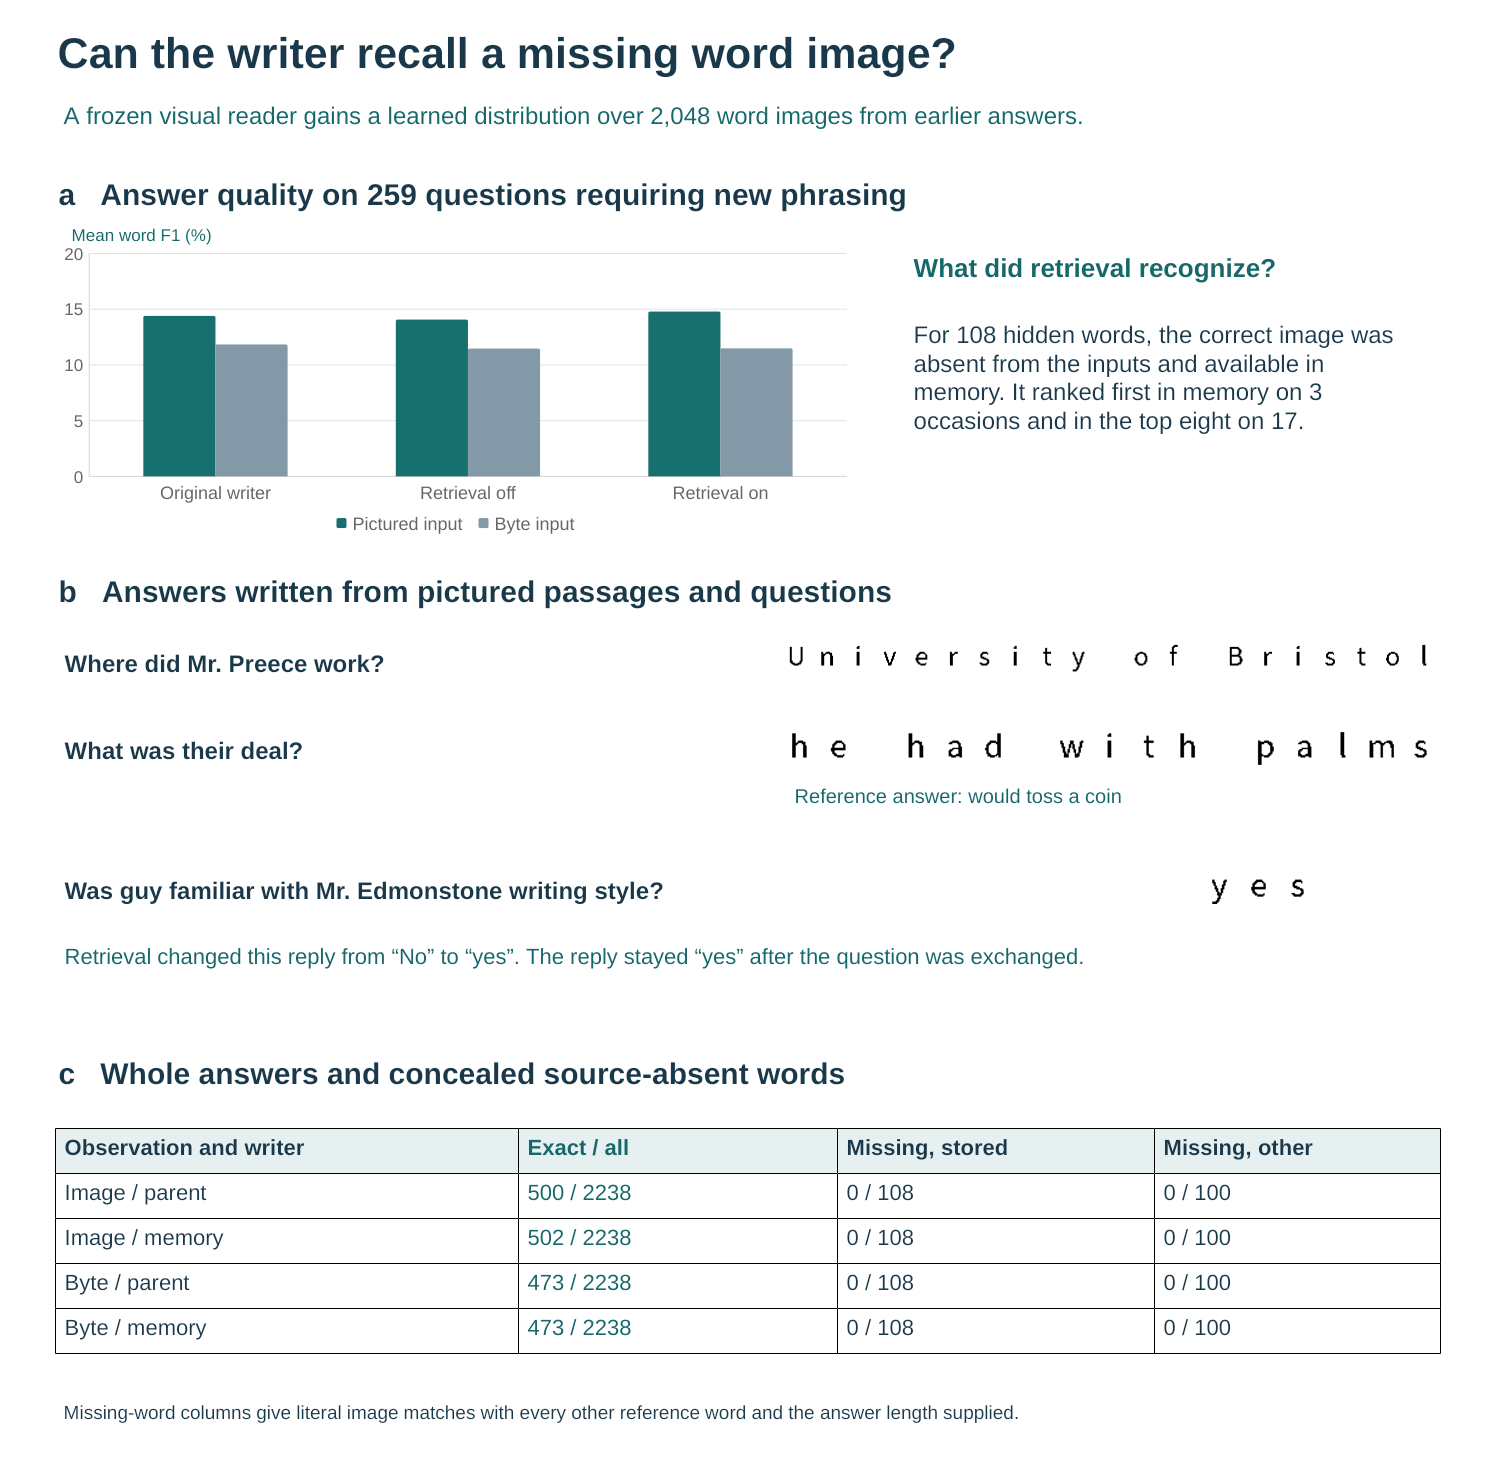
\includegraphics[width=.84\textwidth]{figures/Figure_133_word_memory.png}
\caption{\DIFaddFL{\textbf{Retrieving fitting-word images in a new answer.} \textbf{a,} Mean word F1 on 259 held questions whose normalized target wording is absent from the inputs. All arms produced zero complete matches on this subset. The decoder-only control sets the retrieval gate to zero. Ranks at right use the correct length and other answer words. \textbf{b,} Actual visual outputs reproduced from pictured inputs. Examples follow fixed corpus order within the first source-sensitive multiword success, first difficult miss and first correction relative to disabled retrieval. \textbf{c,} Normalized exact complete answers on all held turns and literal word-image recovery with a single concealed word. Stored denotes membership in the fitting memory. Each main count uses the original passage and question.}}
\label{fig:word-memory}
\end{figure*}
\begin{figure*}[p]
\centering
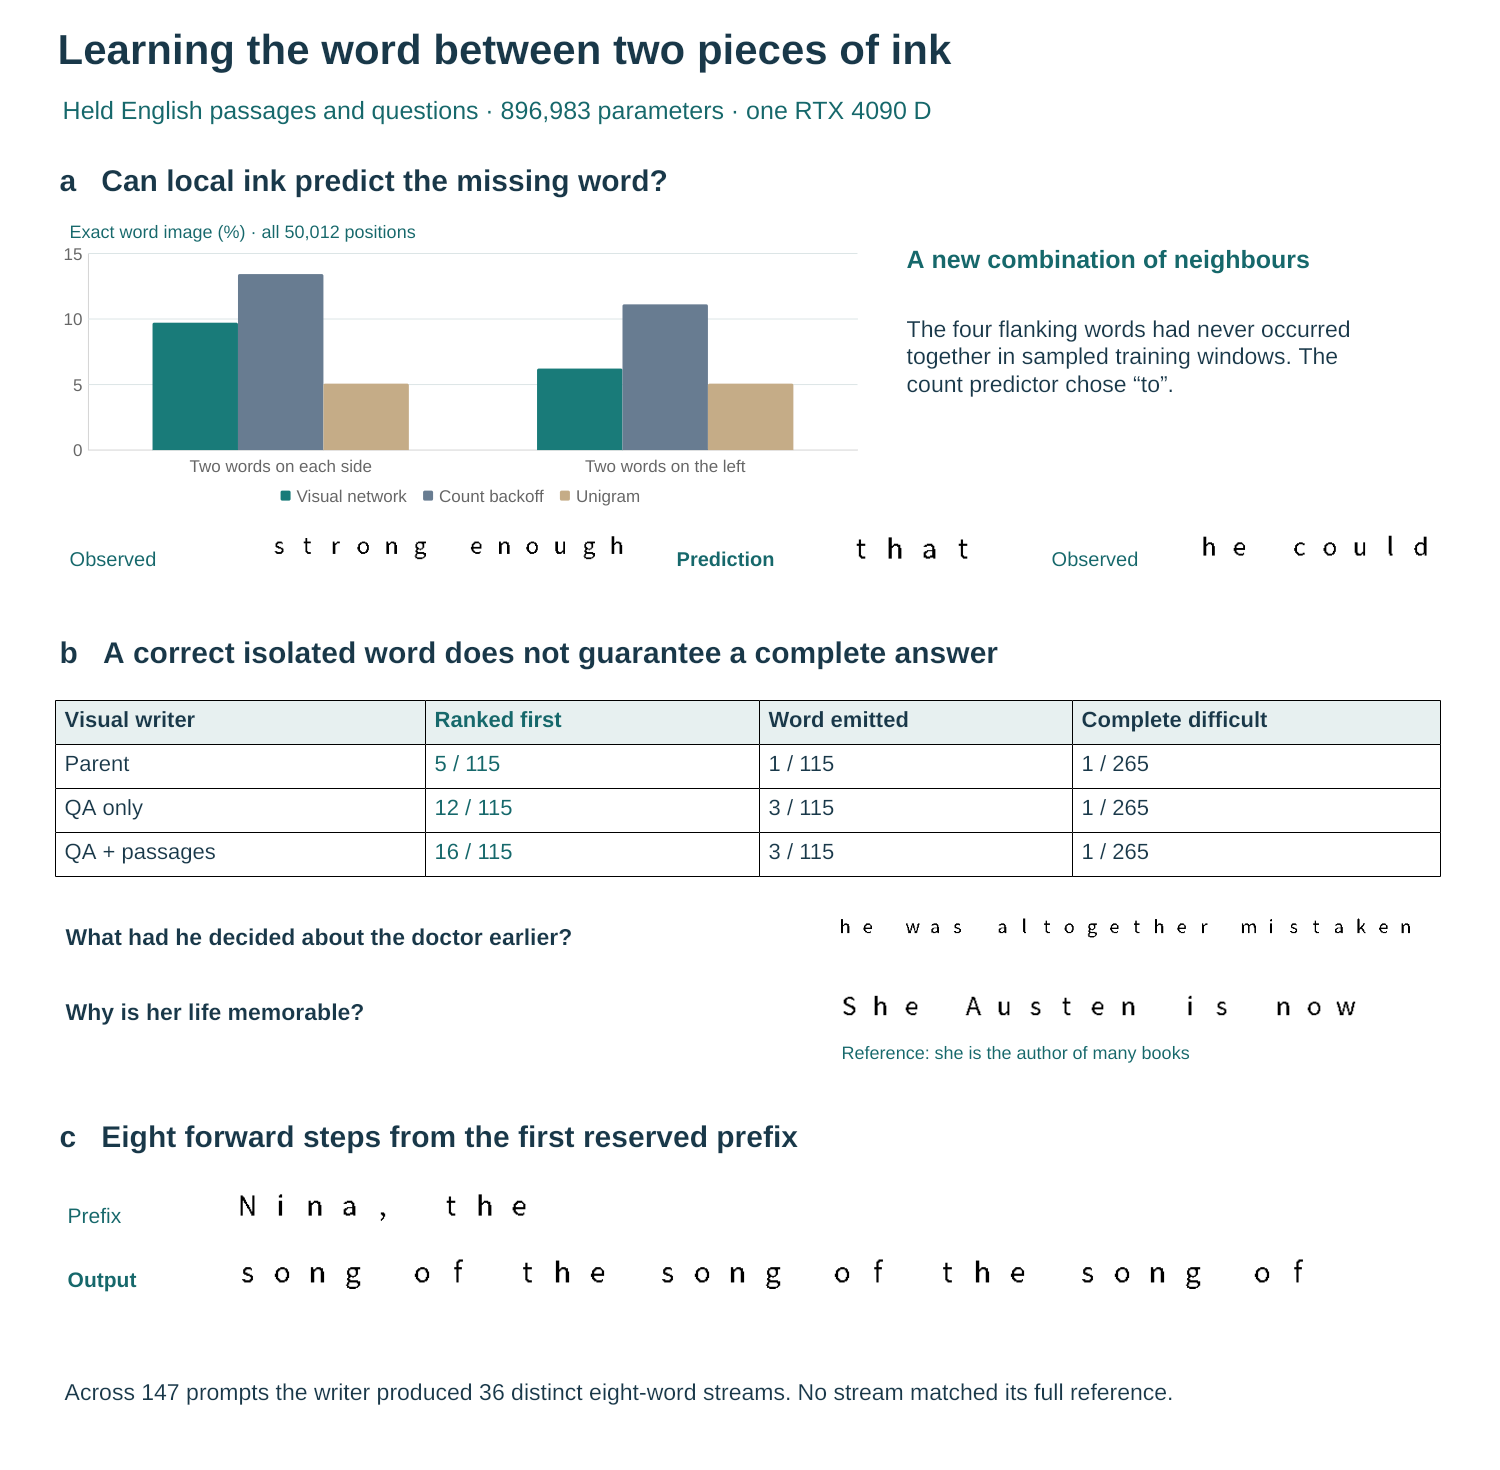
\includegraphics[width=.84\textwidth]{figures/Figure_134_context_cloze.png}
\caption{\DIFaddFL{\textbf{Neighbouring word images predict some missing text.} \textbf{a,} Literal held word accuracy with both sides present and with only the left side visible. The network and count backoff were trained with the same 256,000 passage windows. The image strips show an unseen four-flank combination and the predicted centre. \textbf{b,} Conditional rank and emitted word with reference neighbours supplied, followed by exact autonomous replies on all difficult questions. The first exchange-sensitive difficult success and first difficult miss are shown in source order. \textbf{c,} Greedy continuation from the first reserved passage in evaluation order with no right-hand context. The repeated text is the actual output.}}
\label{fig:context-cloze}
\end{figure*}
\begin{figure*}[p]
\centering
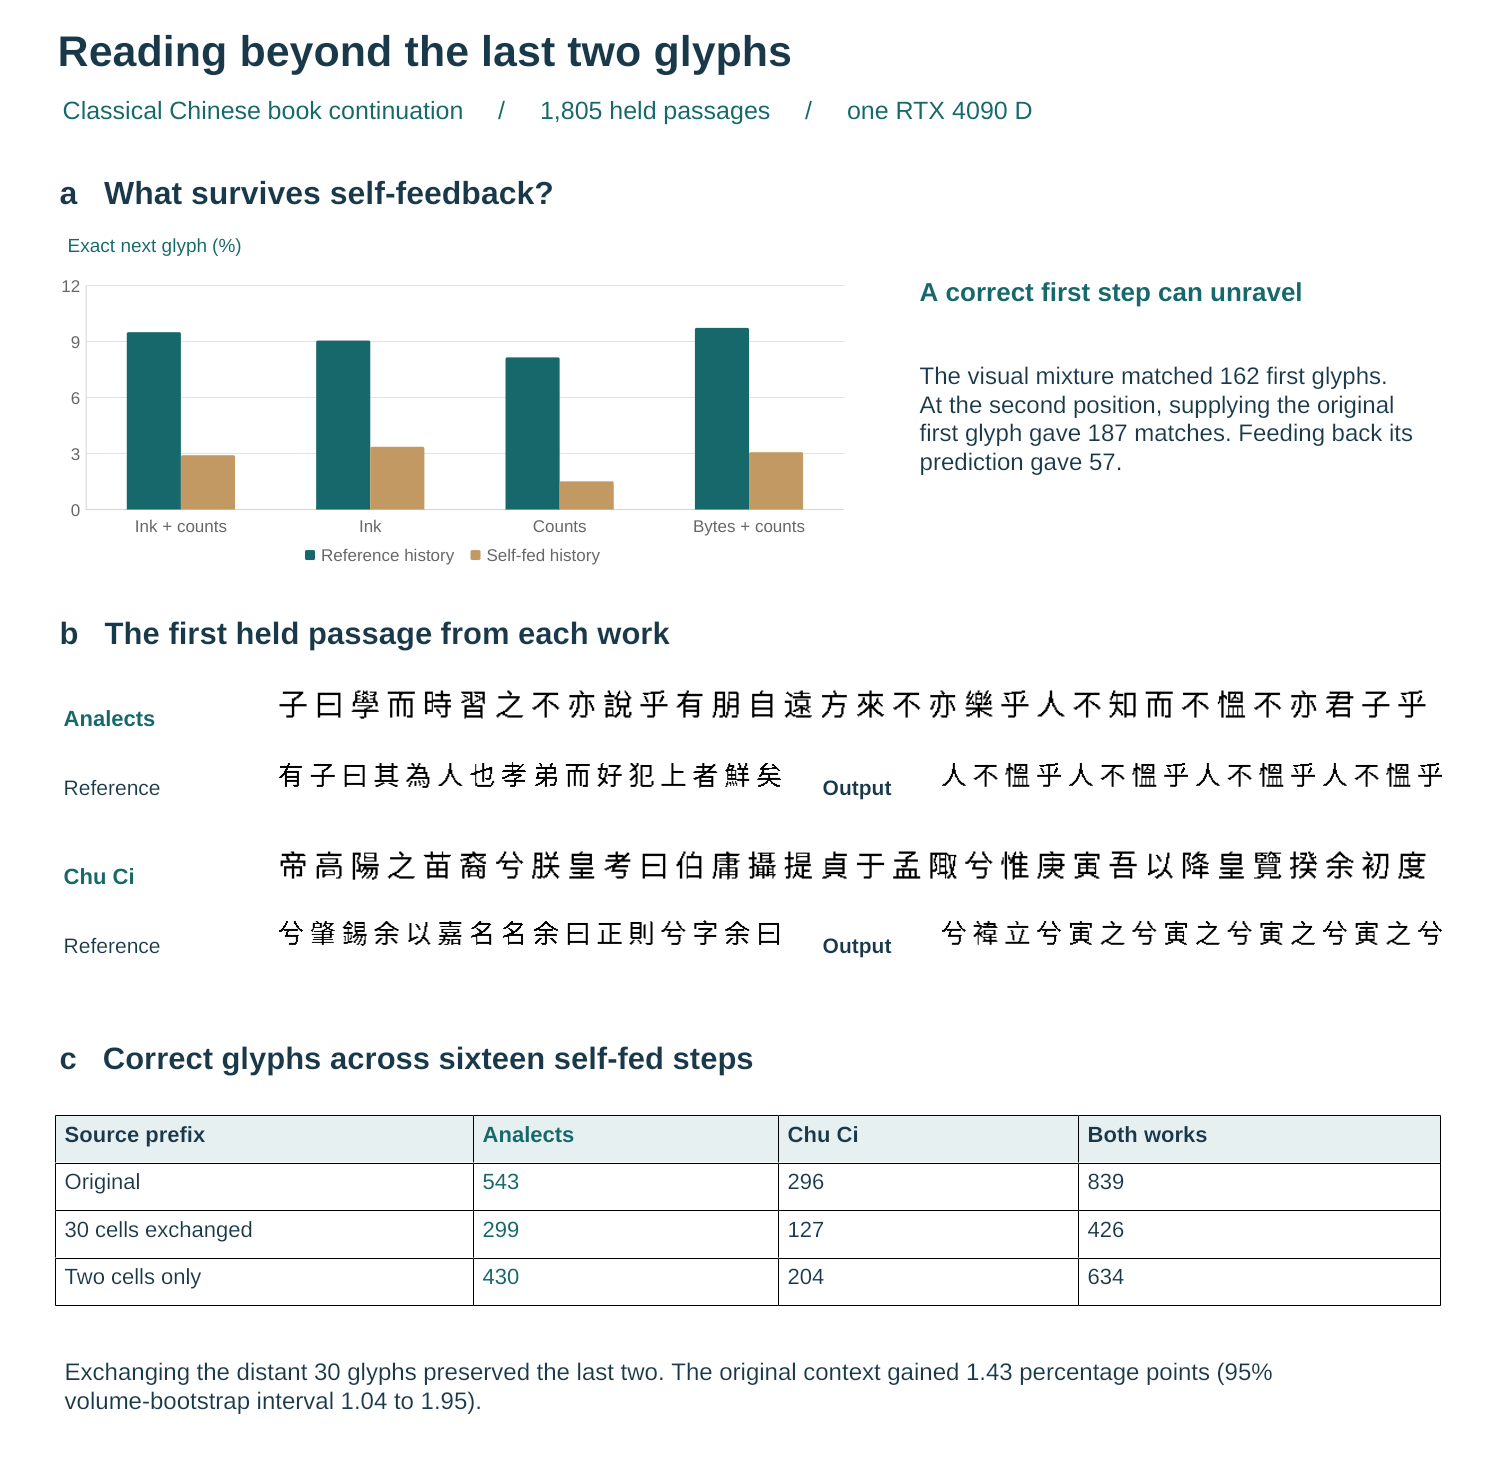
\includegraphics[width=.84\textwidth]{figures/Figure_135_book_prefix.png}
\caption{\DIFaddFL{\textbf{A longer pictured prefix influences autonomous writing in two classical Chinese books.} \textbf{a,} The same 28,880 glyphs were predicted with the source history supplied at every step or with each predicted bitmap fed back to the writer. Each neural writer included a learned pointer to previous cells. \textbf{b,} First test passage in each work, followed by its reference and sixteen physical outputs from the visual mixture. Both examples enter short cycles. \textbf{c,} Correct positions after exchanging the first 30 cells with a passage from the other work or restricting the writer to two observed cells at every step. The intervals resample volumes within each work.}}
\label{fig:book-prefix}
\end{figure*}
\begin{figure*}[p]
\centering

\includegraphics[width=.84\textwidth]{figures/Figure_136_verse_canvas.png}
\caption{\DIFaddFL{\textbf{Visible-glyph supervision and writing from pictured verse.} \textbf{a,} Fraction of previously hidden cells matching the recorded second line across 6,362 line pairs from 156 reserved poet attributions. The masked writers fill one cell per step. The count predictor uses the first-line glyph at the corresponding position. \textbf{b,} First confirmation example in fixed order and first exact two-cell repair that failed after source exchange. The strips reproduce the input, reference and emitted bitmaps. \textbf{c,} Counts for the image writer with identity supervision, including a first line from another poem and an unseen Droid typeface. Surviving second-line ink stays in the canonical face.}}
\label{fig:verse-canvas}
\end{figure*}
\begin{figure*}[p]
\centering
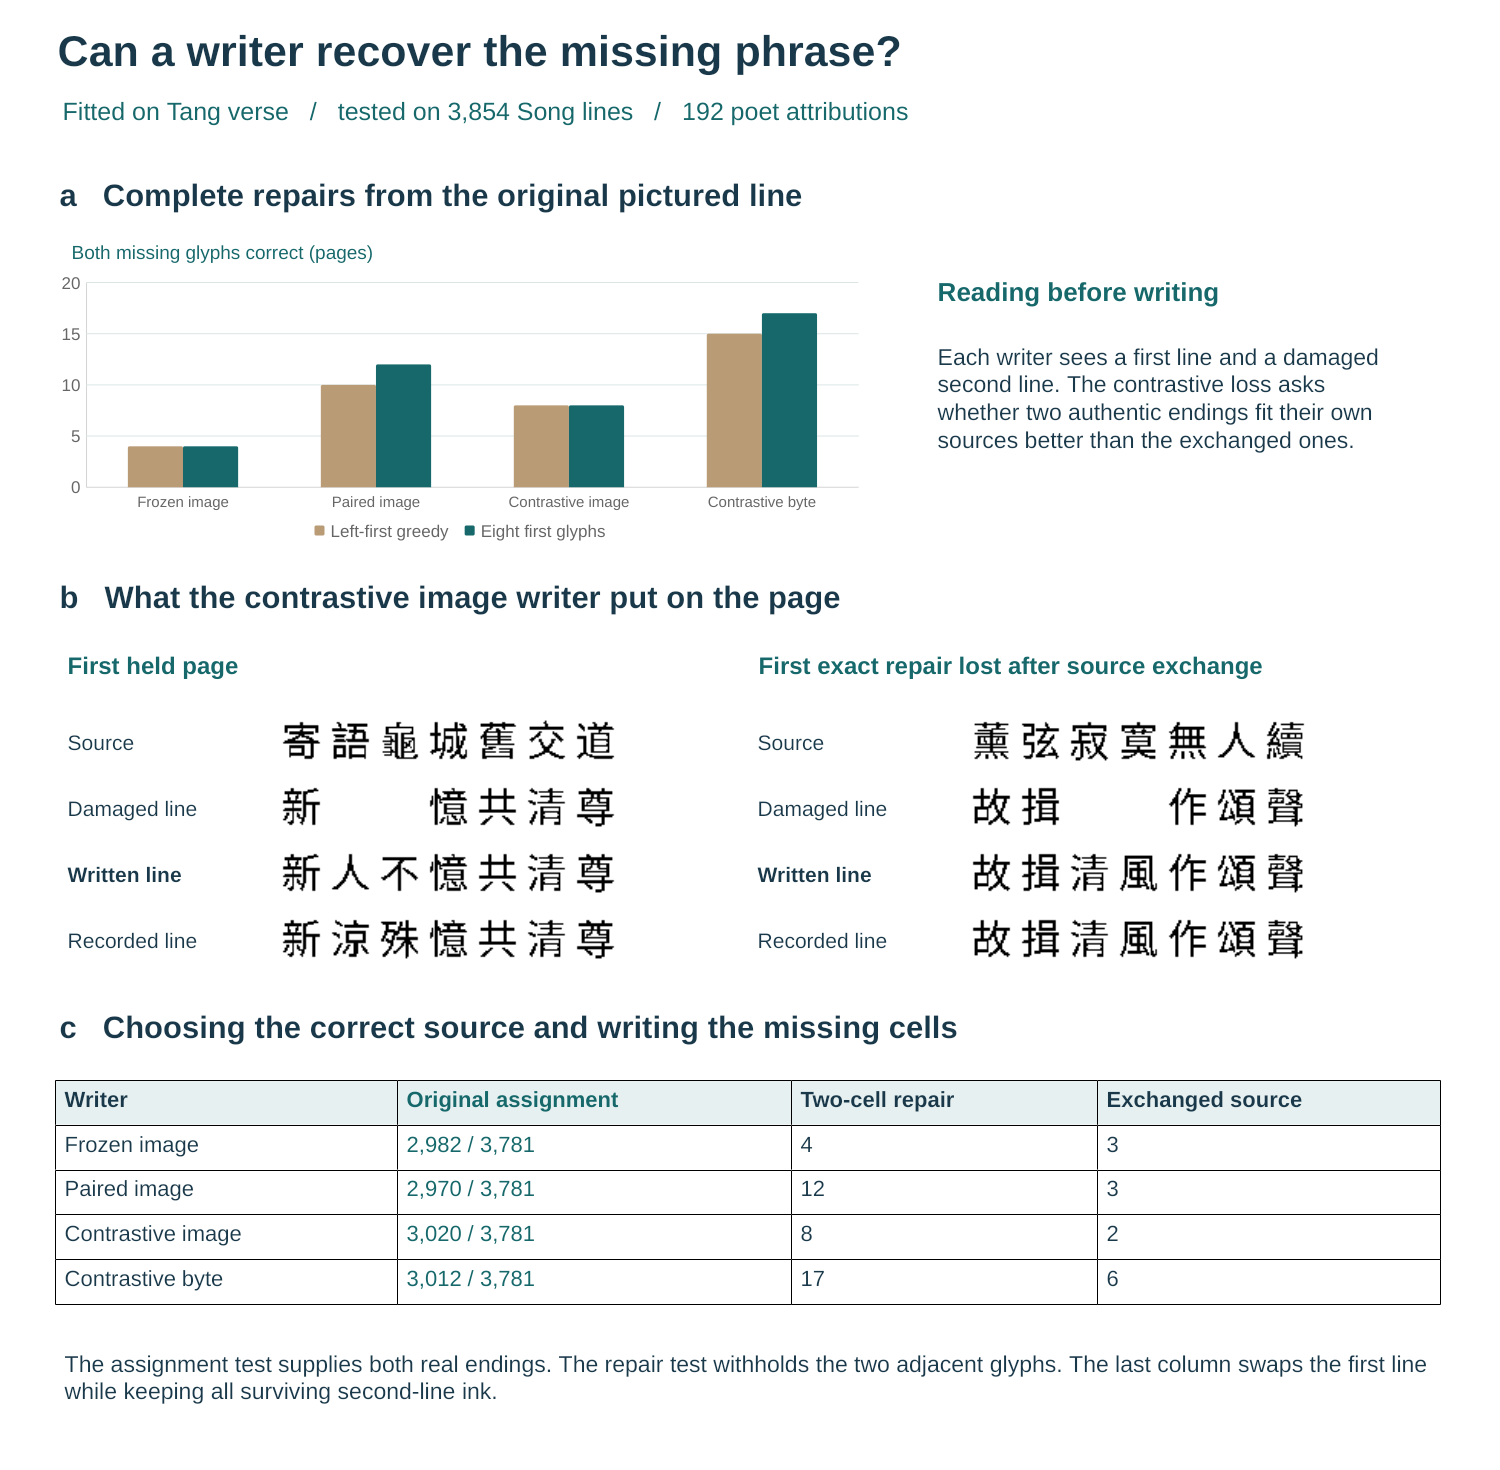
\includegraphics[width=.84\textwidth]{figures/Figure_137_verse_contrast.png}
\caption{\DIFaddFL{\textbf{Source discrimination and recovery of missing glyphs in Song verse.} \textbf{a,} Number of pages on which both missing glyphs matched the recorded line under two ordered decoders. The paired and contrastive writers continue their respective visible-glyph-supervised parents on identical Tang training examples. \textbf{b,} Actual input and output pixels from the first held page and the first exact repair lost after exchanging its source. \textbf{c,} Correct reciprocal assignments among pairs whose reference glyphs are in the output bank, and exact repairs across all 3,854 pages with the original or exchanged source.}}
\label{fig:verse-contrast}
\end{figure*}
\begin{figure*}[p]
\centering
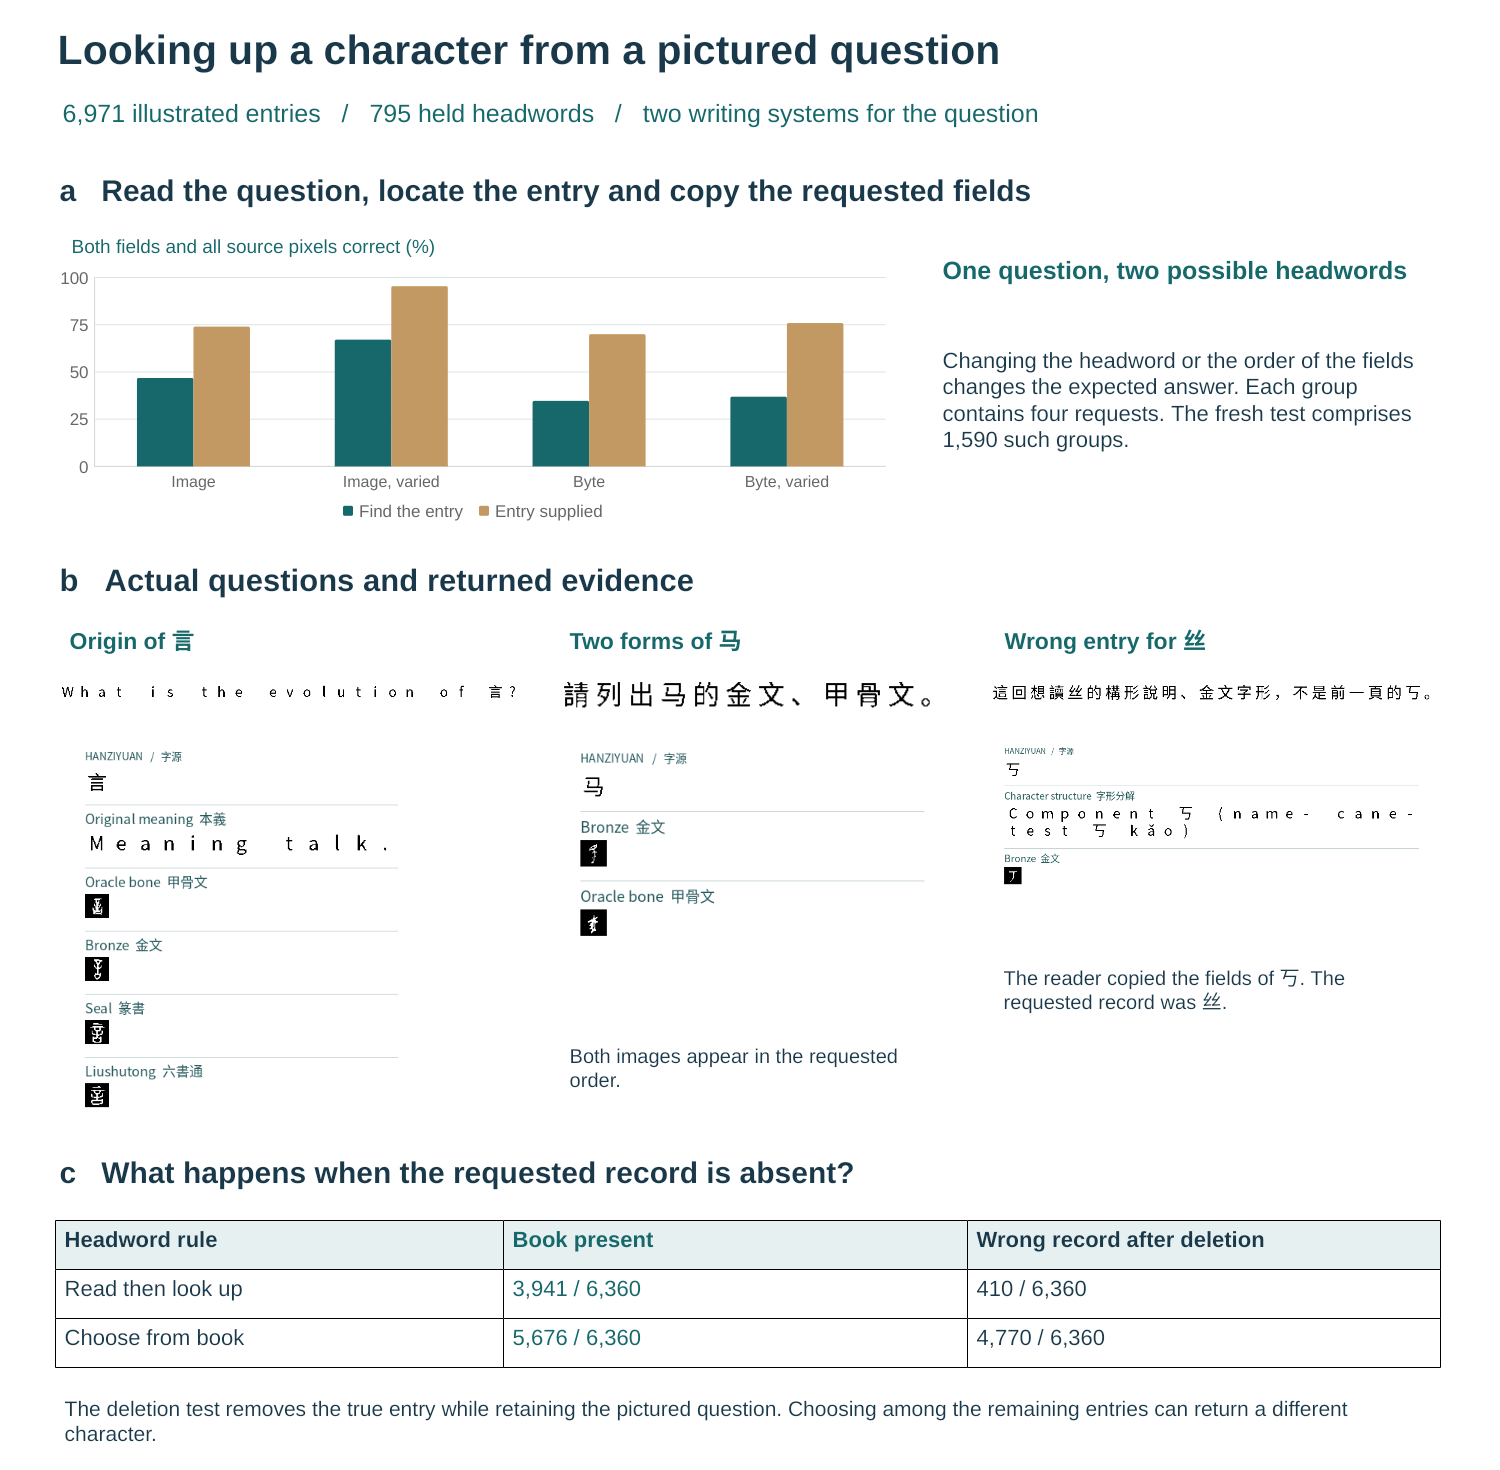
\includegraphics[width=.84\textwidth]{figures/Figure_138_glyph_atlas.png}
\caption{\DIFaddFL{\textbf{Attested character forms returned by a visual question reader.} \textbf{a,} Complete two-field responses to 6,360 held questions with and without the correct entry supplied. Varied wording adds twenty training frames. \textbf{b,} Actual question strips and response images for two successful records and one wrong headword. Each form retains its source pixels. \textbf{c,} Restricting the pointer to indexed headwords improves lookup with the entry present and increases wrong selections after its deletion.}}
\label{fig:glyph-atlas}
\end{figure*}
\begin{figure*}[p]
\centering
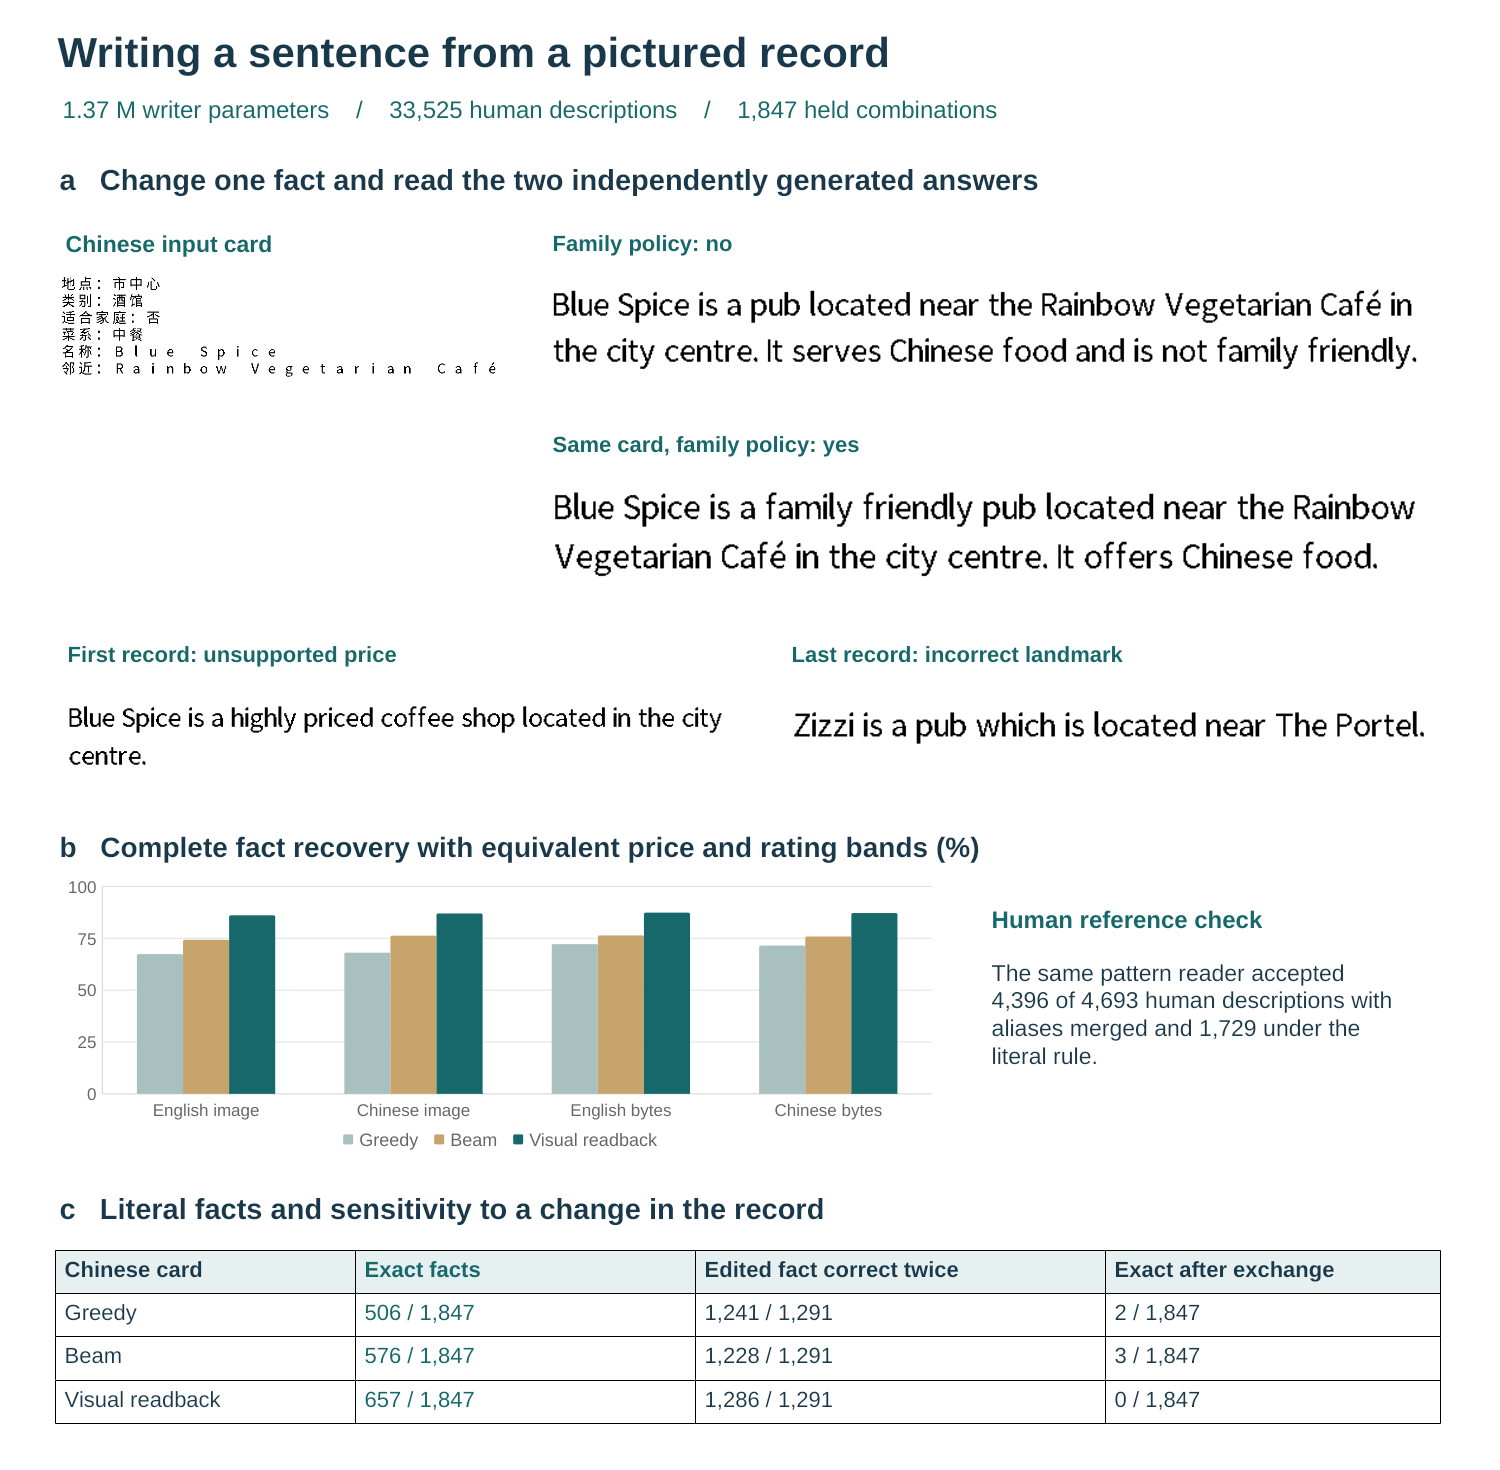
\includegraphics[width=.84\textwidth]{figures/Figure_139_semantic_page.png}
\caption{\DIFaddFL{\textbf{Conditional sentence writing with optical readback.} \textbf{a,} The first held Chinese card with an editable family policy and both complete answers. The price hallucination and wrong landmark below come from the first and last test records. Images retain the actual emitted glyphs. \textbf{b,} Complete observed fact sets after merging price and rating aliases. The same 1,847 held records are presented in each script. \textbf{c,} The stricter literal detector, the direction of the edited fact in both answers, and a one-record cyclic exchange of the original sources.}}
\label{fig:semantic-page}
\end{figure*}
\begin{figure*}[p]
\centering

\includegraphics[width=.84\textwidth]{figures/Figure_140_visual_fact_reply.png}
\caption{\DIFaddFL{\textbf{Writing a requested fact from pictured evidence.} \textbf{a,} Two natural Chinese questions about the same held restaurant and the original machine-written replies. The questions ask for hours and location. \textbf{b,} Percentage of replies with the requested source value and no competing value or extraneous number, with all 515 turns, 384 unseen questions, 69 unseen venues or 59 turns with both unseen. A pictured hotel-type question produced an address. \textbf{c,} A separate English writer uses historical marks as unfamiliar names inside a generated sentence. The table requires both directions in each name-exchange pair to convey the other recognized fields.}}
\label{fig:visual-fact-reply}
\end{figure*}
\begin{figure*}[p]
\centering

\includegraphics[width=.84\textwidth]{figures/Figure_141_two_fact_figure.png}
\caption{\DIFaddFL{\textbf{Learning which fact to express while drawing a clause.} \textbf{a,} Original question and emitted ink from the two visual writers on the same hotel card. The earlier writer interchanged the words for price and address. \textbf{b,} Counts out of 37 held turns for a clean pair of source values and for a clean pair with explicit local property attachments. The guests' original wording sometimes disagreed with the two-field annotations. Qwen read ordinary text. \textbf{c,} Both answers must place the values in the instructed order after the field names exchange places. Eighteen pairs share each wording.}}
\label{fig:two-fact-figure}
\end{figure*}
\begin{figure*}[p]
\centering
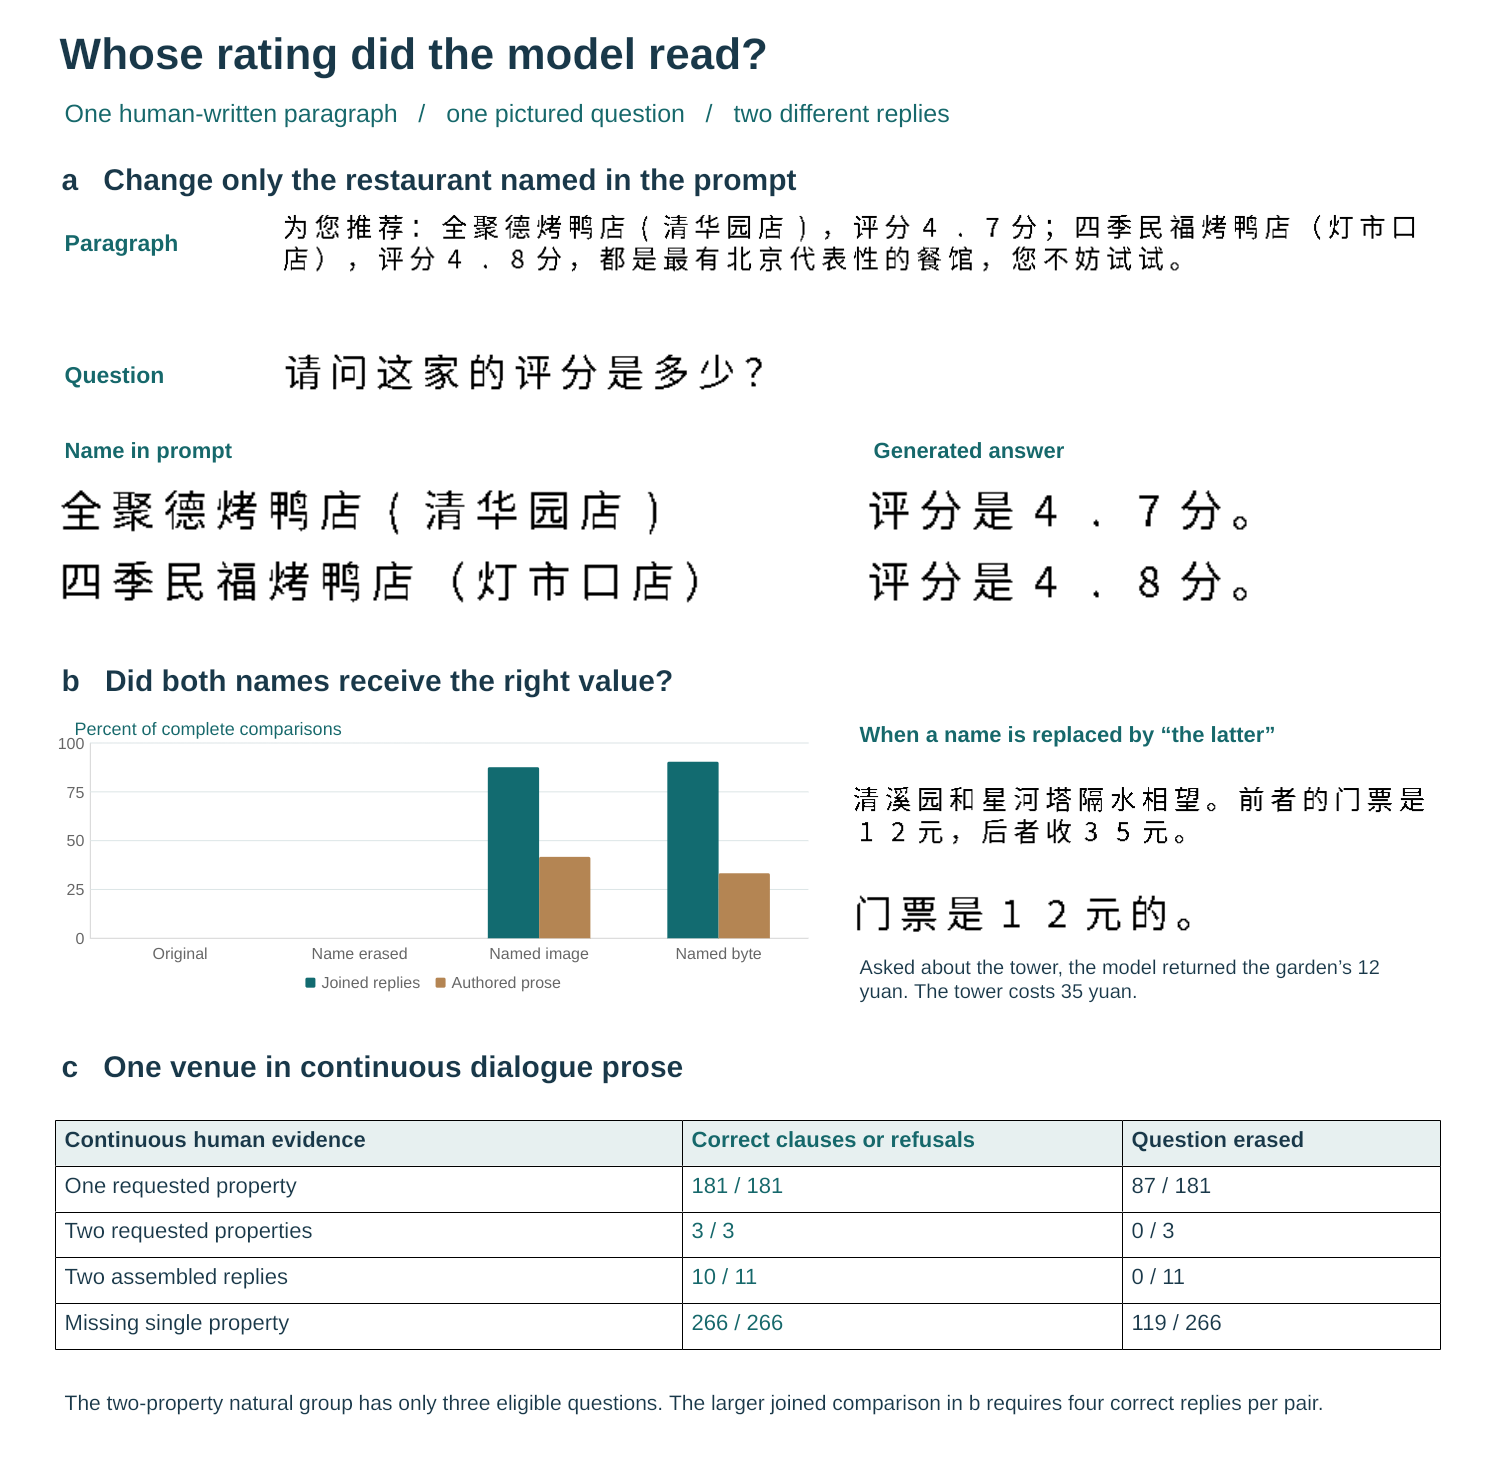
\includegraphics[width=.84\textwidth]{figures/Figure_142_prose_fields.png}
\caption{\DIFaddFL{\textbf{Whose rating is printed in a Chinese paragraph?}
\textbf{a,} The same natural test utterance rates two named restaurants. Changing only the pictured target name changes the emitted rating. \textbf{b,} Both target names must receive their own value. Each of 539 joined comparisons additionally requires recovery under the reverse passage order. Twelve separately authored two-venue paragraphs retain their natural order. The example on the right asks for the second attraction's admission price. \textbf{c,} Source-matched human questions paired with evidence from a different test conversation. Counts use the single-venue model and require a clean literal value with a local property cue, or the correct requested field and missing-value report. Question erasure preserves the paragraph.}}
\label{fig:prose-fields}
\end{figure*}
\begin{figure*}[p]
\centering
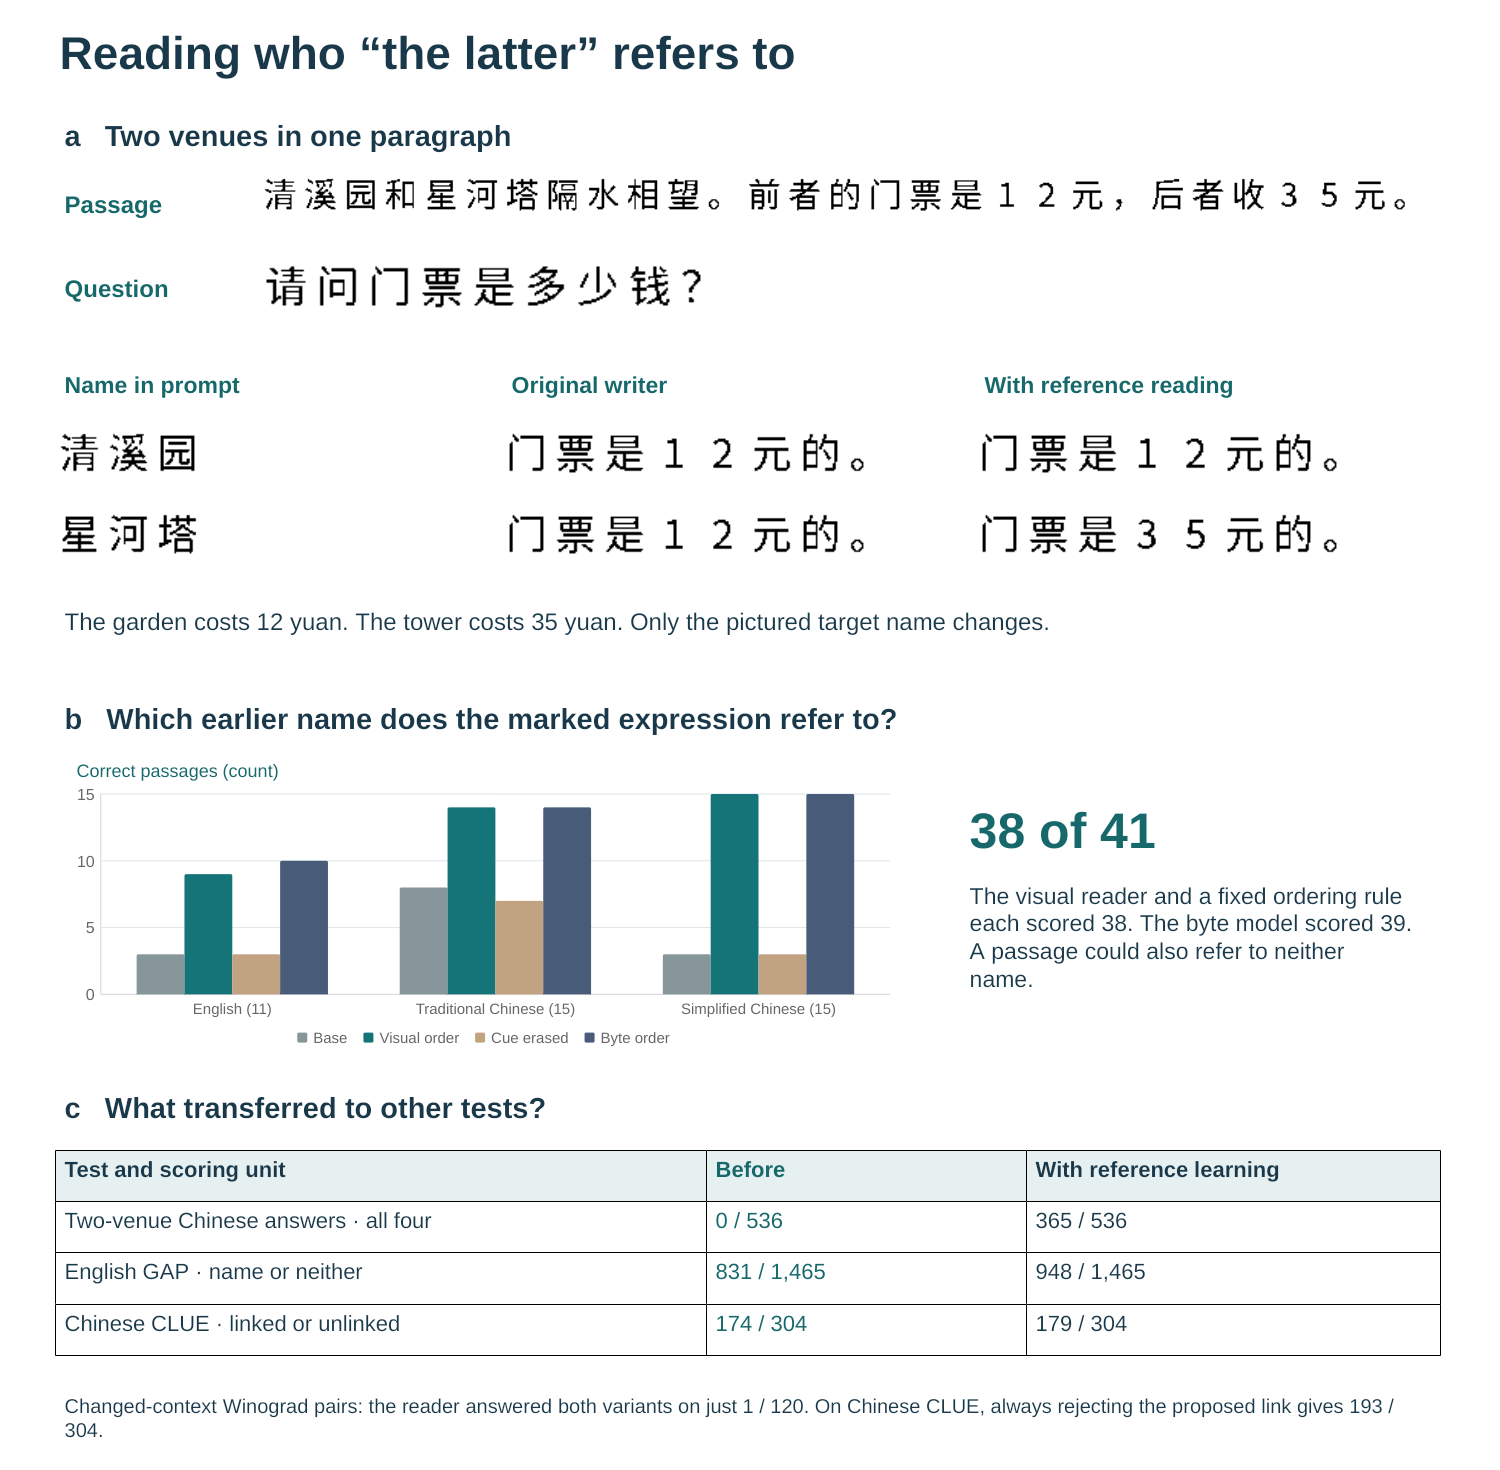
\includegraphics[width=.84\textwidth]{figures/Figure_143_story_mentions.png}
\caption{\DIFaddFL{\textbf{Reading the owner of an indirectly stated fact.}
\textbf{a,} Original paragraph, question, target strips and emitted reply images for the authored park and tower example. The question asks for an admission price. The numerals and their units are printed in the passage. \textbf{b,} Correct referents in screened passages from SQuAD, DRCD and CMRC. The four bars in each group combine the same supplied candidate names with different readers. The post-fit explicit ordering rule solved 38/41. A reader can also select neither name for an adjectival use. \textbf{c,} The Chinese two-venue task requires both names in both orders. The English and Chinese reference tests compare story-only fitting to mixed-corpus fitting of the same visual model. GAP is a three-way choice including neither, whereas CLUE tests one proposed link.}}
\label{fig:story-mentions}
\end{figure*}
\begin{figure*}[p]
\centering
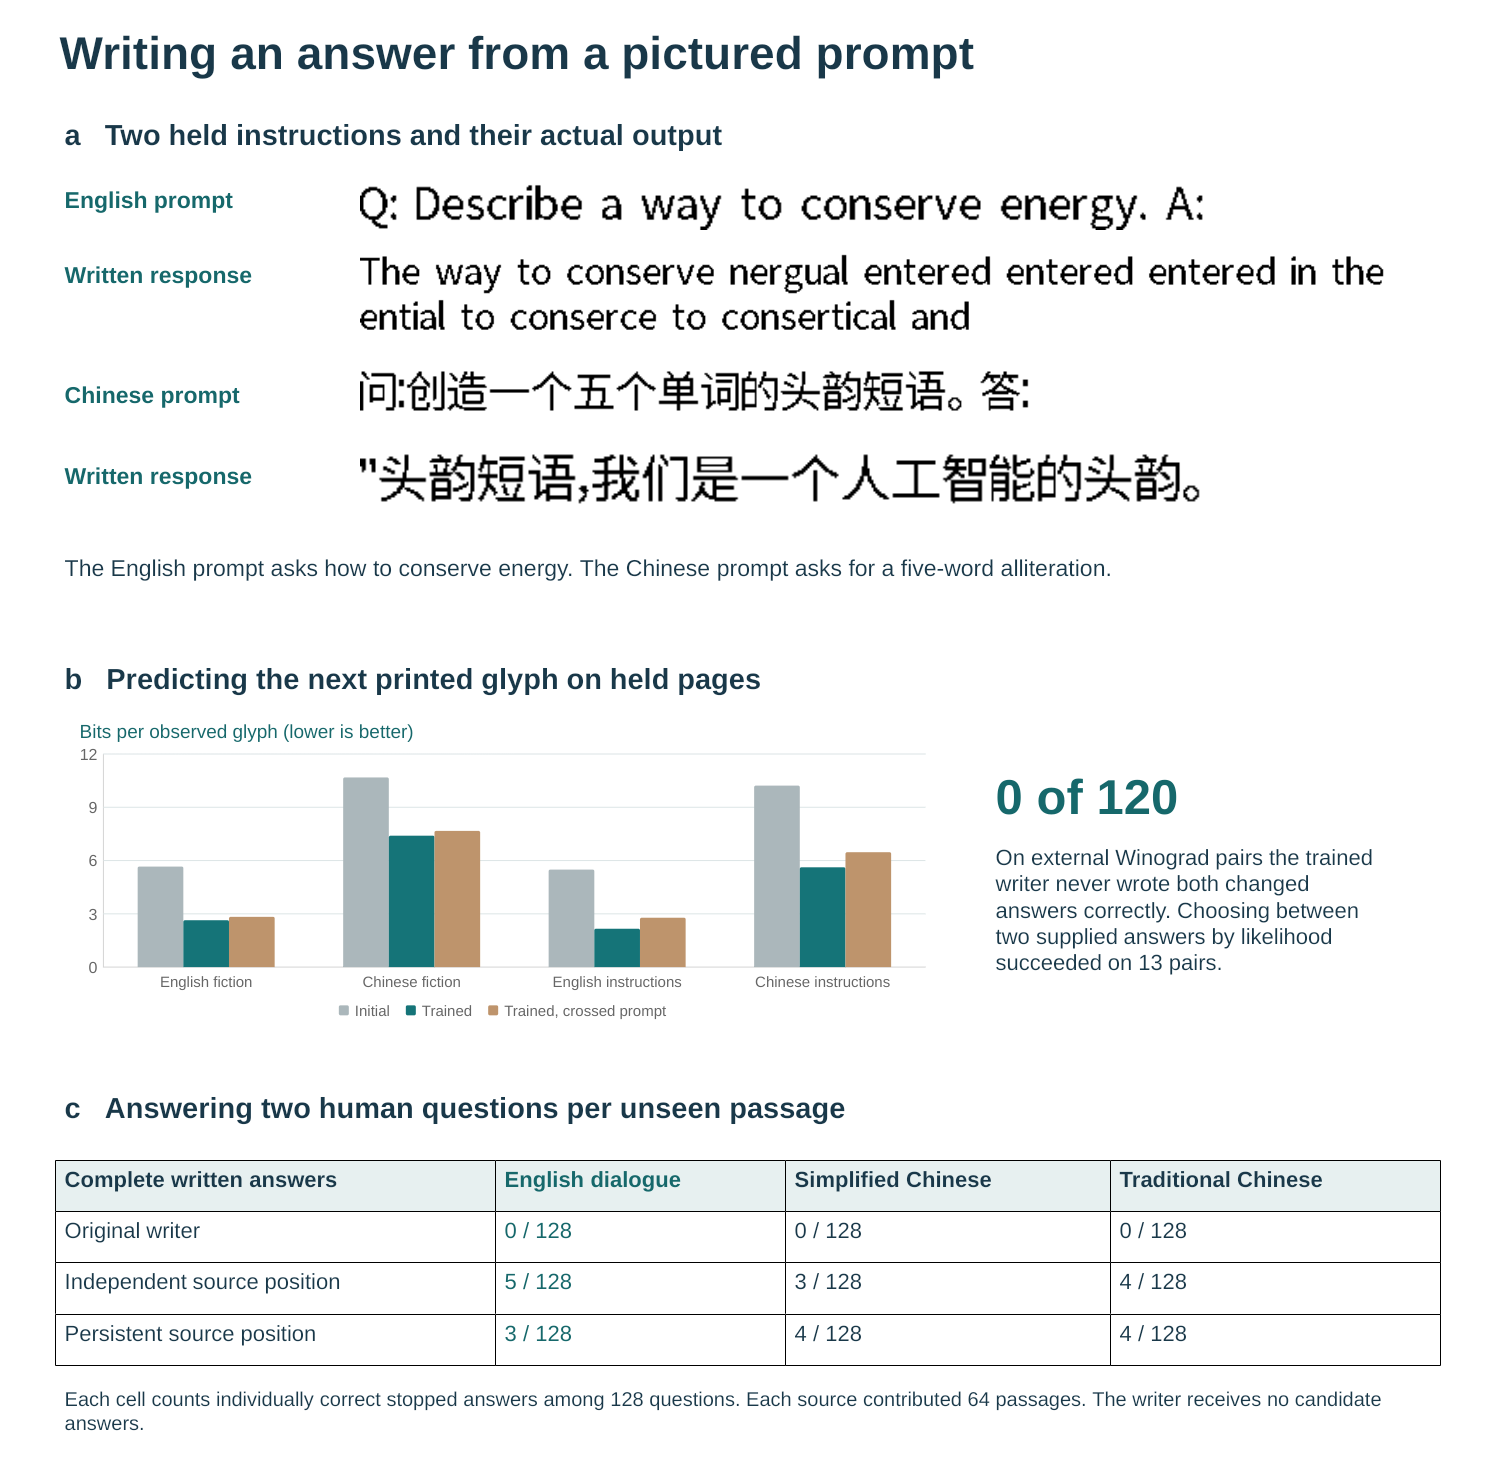
\includegraphics[width=.84\textwidth]{figures/Figure_144_visual_discourse.png}
\caption{\DIFaddFL{\textbf{Predictive learning and open writing from glyph images.}
\textbf{a,} First held English and Chinese instructions in fixed hash order with the paired writer's own emitted pixels. Blank sidebearings and line wrapping have been adjusted for display. The English output reached the 96-cell limit. \textbf{b,} Mean held next-glyph cost with correct preceding answer cells. The four groups contain 128, 24, 128 and 128 windows. Crossed prompts are from the same task and language. The Winograd count requires writing both opposite correct names and stopping. \textbf{c,} Complete self-generated answers on human questions from CoQA, CMRC and DRCD. The two source-position models shared their base and fitting draws. In each corpus two different questions refer to each of 64 unseen passages. No model wrote both correct answers on any passage.}}
\label{fig:visual-discourse}
\end{figure*}

\clearpage

\DIFaddend \section*{Discussion}
%DIF >  Active article input; prior staged versions remain in Git and validation receipts.
\DIFaddbegin \subsection*{\DIFadd{Conditional writing and complete language}}
\DIFadd{The complete continuation trial does not resolve the visual language problem.
Three epochs over complete targets yield some correct short answers, but the
final proportional model gives 7/32 strict complete answers, no both-correct
pair and no credited coherent complete book continuation. The three-quarter
checkpoint's 9/32 exact answers do not replace the prescribed final model.
The final model also loses two required proportional successes and fails the
normal-minus-erased contrast. Both pilot audits reject it. More unchanged
epochs or selecting an intermediate peak would not explain this failure.
}

\DIFaddend The \DIFaddbegin \DIFadd{supplied-history controls narrow the interpretation. At the final
checkpoint, 656/713 later proportional QA predictions reach foreground F1 0.95
under correct preceding images and supplied lengths. Sampled training books
reach that level on only about 9\% of later positions. These are physical
comparisons against canonical targets, with predicted stopping bypassed;
they do not qualify autonomous answers or align alternative correct wording.
They also make a feedback-only explanation insufficient: book writing remains
inaccurate even when generated history is removed. Reading access, the relation
between contextual states and writing, uncertainty over plausible continuations
and stopping can still contribute to failure.
}

\DIFadd{The saved trajectories reveal dense writing rather than a loss of every
prompt-dependent state difference. Final normal long-book streams place
98.12\% of emitted tiles above the clean training-book 99th-percentile ink
count. All available first-state contrasts remain unequal. The restricted
context-independent optimum of the balanced writing loss produces a dense
thresholded template, but this is not the optimum of the conditional neural
model and does not prove an attractor or unique cause. A state difference
likewise does not establish question understanding. Complete outputs and
controlled prompt interventions remain the decisive language evidence.
}

\DIFadd{The subsequent head-only comparison replaces thresholded marginal pixels with
a normalized distribution over each complete glyph, preserving the final
reader, continuation dynamics, feedback encoder and stop head. Its 128 physical
eight-pixel masks enumerate local patterns rather than character identities;
all $2^{1024}$ binary rasters remain representable. Original frozen physical
credits rise from 599/1,040 to 970/1,040, but two candidate groups fail the
unchanged prerequisite. The later pixel audit finds seventeen blank-flag
disagreements, including four credited empty images. Original scores remain
frozen with that limitation, not interpreted as corrected physical accuracy.
No autonomous language result is assigned to this failed actor.
}

\DIFadd{The exact probability diagnosis further narrows the intervention. Only sixteen
of 349 false blanks prefer their source over the empty image. The selected
book/training-QA search-only criterion fails, and a first-nonzero-prefix bound
supports an empty mode for fifteen of 42 development-book false blanks, subject
to finite-precision arithmetic. These measurements do not prove that every
search alternative is bad, but they do not justify search alone as the next
repair. The completed context-gradient fit instead lets the query and
continuation residuals learn through the same image likelihood, with balanced
stop loss retained. It lowers source NLL, yet all book groups fail qualification
and complete-array book false blanks rise from 324 to 689. A second opaque
review also contains contradictory blank flags and credited empty images; its
original outcomes remain frozen. The actual-context probability study supports
108 empty global modes and rejects its prospective search-only rule. It does
not prove that empty modes explain every language failure.
}

\DIFadd{These measurements distinguish density learning, recognizable marks and correct
writing. The completed whole-glyph ranking comparison reduces false blanks from
711 to 37 and passes all seven readable-form groups. Exact source-bitmap matches
increase only from 4,603 to 4,609 of 12,597 positions, while false ink at genuine
whitespace increases from eleven to twenty-five. Fixed-order samples retain
simple marks that differ from their sources (Fig.~\ref{fig:ranking-completed}).
Source-over-blank ranking compares two complete paths; it does not bound the
probability of other nonempty modes. This limitation is consistent with the
observed marks without identifying a unique cause of language failure. Bitmap
mismatch is itself a fidelity diagnostic, not a complete-language judgment.
}

\DIFadd{The complete saved-score comparison makes that distinction measurable. At
7,206 of 7,926 nonempty bitmap mismatches, the emitted image already has higher
probability than the source by the fixed margin (Fig.~\ref{fig:glyph-score-gaps}).
That witness excludes the source from the highest measured score at those
positions, without establishing a global optimum for the emitted image or a
unique cause of failure. A source-directed search alone cannot explain these
canonical mismatches. Conversely, forcing every reference-book glyph to be the
mode would not establish useful language: another complete continuation may
be valid. Conditional source-mode learning remains a candidate for later
controlled testing alongside complete prompt-based language evaluation. The
subsequent white-target fit tests the separate blank condition.
}

\DIFadd{The fixed complete-density blank comparison fails its prospective repair rule.
An added blank-target term instead trains a sufficient upper-bound condition
for blank global optimality at genuinely empty sources. Its six-case reset
full-body preflight passes at 17.795 GiB, including complete sources with actual
whitespace. The complete registered comparison then reduces false ink from
25 to 12, but produces 54 false blanks instead of 37 and fails both fixed limits
(Fig.~\ref{fig:white-target-completed}). Every additional false blank occurs in
books. The bound may be loose and stronger blank pressure may erase nonempty
forms, but these observations do not identify a unique causal mechanism.
The construction still has 5,005,760 trainables within 7,553,448,370 total
parameters. Neither a normalized physical density, a readable mark nor a
gradient check establishes a lightweight foundation or semantic understanding.
Complete prompt-dependent answers remain necessary.
}

\DIFadd{The reward controls expose a further requirement for whole-answer learning.
A scalar image resemblance score can rank an uncertain output above a known
correct answer, while a disjoint geometric decoding rule can abstain on readable
correct cells and accept an uncertain sequence (Fig.~\ref{fig:reward-calibration}).
Neither result identifies which interpretation of the uncertain sequence is
true. Both preserve the original review and reject their proposed training
rewards. A training-only judge must account for complete emitted contents,
order and stopping before its feedback can justify a judge-derived policy fit. The
finite prototype inventory remains outside deployment, and the proposed
whole-answer policy component has not produced a language-learning result.
The later fixed vision reader and frozen image-feature metric also fail their
prospective requirements. Exact source rendering does not make isolated raw
Unicode labels identifiable when distinct characters share pixels. These
failures preserve uncertainty and do not show that all vision readers or
contextual visual learning are impossible.
}

\DIFadd{Direct supervised learning from authentic images and saved training-only
teacher states remains available without a qualified reward judge. The selected
comparison lets the compact model's entire inherited contextual body learn,
keeping its reader, writer, complete corpus and objectives matched. Six real
update/reset trials establish gradients, optimizer arithmetic and memory
support, not semantic understanding (Fig.~\ref{fig:visual-context-evidence}).
Its 1,465,381,142-parameter deployment is smaller than the earlier actors but
inherits text pretraining. After the complete fit, the learned body stops on every long book prefix.
Neither arm produces a readable complete answer on this cohort
(Fig.~\ref{fig:full-context-comparison}). The experiment therefore supplies
no matched-quality estimate of language-learning efficiency. Earlier smaller trainable
bodies failed, so trainability alone is not a sufficient explanation.
}

\DIFadd{Resource claims concern the entire deployed system. The evaluated full
point-writer model retains 7,578,390,003 parameters, including its inherited
7,522,463,984-parameter visual/contextual body. Its bounded one-4090 execution
does not show that this body can be learned on that device or that it is more
efficient than a text model at matched language quality. Data preparation,
inherited pretraining, failed attempts, training, generation and review remain
separate costs. The small compact-model trials also fail their language tests;
low memory use alone does not satisfy the objective.
}

\DIFadd{The completed continuation comparison reuses a development cohort, with one
model reviewer familiar with that cohort and no independent human adjudication.
Strict canonical mismatch is not necessarily semantic error, and uncertain
readings remain uncertain. The current font and cell resolution do not establish
handwriting transfer, raw-page reading, arbitrary historical-form generation,
general instruction following or etymological accuracy. Any development gain
must survive untouched works and passage groups, natural stopping, independent
execution and whole-model accounting. Extending verified language to historical
and unencoded writing remains the intended application, not a consequence of
pixel support or supplied reconstruction alone.
}

\DIFadd{The compact reader permits a direct test of order at modest training cost.
After 2.57 million next-image targets, its sentence preferences remain
compatible with chance across the sampled Mandarin constructions. Better
code density can reflect more accurate prediction of a glyph's internal
shape. The ordering test asks whether the visual history helps choose among
complete sentences with the same ink. Its negative result leaves an efficiency
advantage at useful language quality unestablished.
}


\subsection*{\DIFadd{Earlier interfaces and conditional-writing controls}}
\DIFadd{The }\DIFaddend results separate a useful visual predictive state from a useful visual
language generator. The established causal reader learns context-dependent
next-writing information, while subsequent writers can erase that information
or model the marginal appearance of glyphs. A complete visual language model
must bind meaning and sequence to the exact marks it generates.

The compact complete-sequence fit adds a larger authentic target stream while
keeping the contextual foundation fixed. It completes training within one
4090 but does not produce a credited readable complete answer on its fixed
development cohort. Its independent cold replay verifies execution boundaries,
not comprehension. The velocity projection has a provable noise subspace;
terminal normalization also matters when repairing its width. The completed
wider-writer comparison removes the tested restriction but retains zero
complete exact QA answers at every checkpoint. Correct-history diagnostics
show writing failure before generated feedback, while a separate reader
restriction limits native-target alignment. These results reject the unchanged
joint recipe and a sampler-only repair. The \DIFdelbegin \DIFdel{next model decision requires a matched-cohort readable control, followed by fresh }\DIFdelend \DIFaddbegin \DIFadd{matched earlier-actor control
retains two exact answers and one fully correct question pair on the same
cohort. Full proportional prompts raise exact answers to six but lose that
pair and an earlier readable answer, failing the registered retention rule.
This establishes presentation sensitivity and limited inherited transfer,
without establishing a consistently better interface or new learning.
The matched native continuation gives ten exact proportional answers from
the same adapted first states, while its lexical decoder remains outside the
ILM. Native reading also depends strongly on layout. All first target forms
have primitive coverage and supplied reconstruction is nearly exact, yet some
original first forms are already damaged. Canonical pixel mismatch can also
reflect readable strokes or different wording. Neither missing first forms
nor later feedback alone explains every failed answer. A direct-context
conditional motor gives seven proportional exact answers but retains only
five of the earlier six, failing its registered pilot. Its cached-state
writing errors persist on training positions. The paired late-time decoded
loss also fails both physical gates. Its local endpoint estimator is trained
on noise/target interpolants; this does not directly supervise the endpoint
reached by its own numerical rollout. Differentiating through that full
rollout improves first-position writing but still fails the later-position
gate. A separately qualified deterministic writer reproduces all 64 selected
training glyphs exactly, yet retains six proportional exact answers and no
both-correct pair. All its initial reader states match the parent. This
training-state pass does not establish transfer to autonomous language, and
the complete comparison fails its pilot. Reader access, conditional writing,
stopping and generated-history drift remain distinct possible restrictions;
these controls do not identify a unique cause. Further model changes require
tests that separate them, followed by untouched }\DIFaddend source groups and independent
review after any development improvement.

An image interface enlarges the representable output space, including the
possibility of forms absent from a character encoding. It does not remove the
need to learn syntax, knowledge or long-range dependencies. This study has not
demonstrated general instruction following, etymology answers, handwriting
transfer or arbitrary historical-script generation. It also lacks independent
training-seed replication and a capability-matched text-model comparison.
Small allocated memory in a bounded experiment establishes feasibility on one
GPU, rather than a general efficiency advantage over language models.

Supplied-target reconstruction is preserved by an aligned inverse-image path;
the free image writers still fail reliable new prompt-directed copying. The separate
source-pixel component passes its new-copy test but fails natural-reading
qualification. The remaining test is whether context selects and generates a
coherent written future. Low teacher-forced
image NLL can reflect dependencies among strokes already revealed within the
target, while generated output still loses global identity. Joint training
improves proper likelihood beyond matched extra density training; the raw
generated continuations still fail the intended language test. Conditional
continuation and short answers require counterfactual prompts and the same
context effect during autonomous sampling and visible feedback.
Broader books and offline teacher-generated exercises can supply later
training data while leaving the final inference path independent. A larger
corpus or longer training requires improvement on the intended generation
task, beyond the conditional-likelihood gain established here.

Broader pixel training reproduces 495 of 512 answers but still fails the
supplied unseen reference images. The matched native reader retains useful
answer capability, directing the intervention toward the learned writing
interface. The complete-glyph loop supports restricted input-dependent date
composition, with actual-image feedback independently replayed. It remains
unreliable on broader questions: eleven of sixteen normal Chinese streams cap.
Wider semantic readout coverage and robust generated histories remain
necessary; clear familiar glyphs and low training loss are insufficient.


Recent visual generators study mixture assignment and the geometry of
distribution matching\cite{mgflow,semot}. These results motivate more expressive
writing distributions, but marginal image fidelity cannot certify an answer.
A generator that swaps the correct images for two equally frequent questions
preserves the answer-image distribution while answering both incorrectly.
Conditional supervision and prompt interventions therefore remain necessary;
natural-image gains do not establish a shortcut to language learning.

An inherited visual/contextual successor provides a separately measured
execution route. With its vocabulary module removed, the complete 7.548B
actor trains 25.58M adapter/writer parameters within 17.181 GiB allocated
memory. Causal, backward and resume checks pass after explicit precision
repairs. Eight short source-engine sanity cases support the contextual
initialization; no image-language ability follows from that check. Its
continuous writer fails its reconstruction test (Supplementary Note 23).
The separate qualified codec preserves supplied writing, while the completed
predicted-code actor fails its autonomous language test
(Supplementary Notes 25--28).
Poor first-block and exact-history predictions, including on training cases,
show that generated-history drift cannot be the sole explanation.
Conditional feature information, readout capacity, the objective and
optimization remain possible limitations. The current evidence does not
select a successful density, optimizer or semantic-transfer method.
External pretraining remains part of the model's provenance.

\section*{Methods}
\subsection*{Compact continuous glyph feedback}
The compact experiment receives ordered $32\times32$ binary ink tiles, with
one fixed Noto Sans CJK face during data preparation. The fixed codec maps
each tile $I_j$ to $z_j\in\mathbb R^{768}$. A 384-channel image encoder uses
learned boundaries to group at most sixteen glyphs. It predicts one to three
continuous updates $u_{i,r}\in\mathbb R^{2048}$ per span. The frozen 28-layer
contextual body consumes those vectors directly and supplies the state $c_i$
after each span. During training, native source alignment supplies span ends
and update counts; at inference both are derived from visible pixels.

The writer predicts length $K\in\{0,\ldots,16\}$ from $c_i$. Length zero ends
generation. For a nonempty span, a conditional rectified flow starts from
$z_0\sim\mathcal N(0,I)$ and applies eight Euler steps,
\begin{equation}
 z_{k+1}=z_k+\tfrac18 v_\theta(z_k,k/8,c_i),\qquad k=0,\ldots,7.
\end{equation}
The codec decodes the endpoint into binary ink. The same image encoder reads
these actual emitted pixels to update contextual history. No font renderer,
OCR service, lexical head or answer lookup supplies generated content. The
128-glyph budget can stop before a full predicted span would exceed the cap;
that stream is recorded as budget-limited rather than naturally stopped.
Raw page segmentation and arbitrary reading order are outside this tile-stream
experiment.

\subsection*{Six complete-sequence objectives}
The reference-image training history differs from generated-image history at
inference. Each complete sequence supplies all continuation/answer spans and
its terminal decision. For predicted feedback vector $\hat u$ and compact
source embedding $e$, the relative regression objective is
\begin{equation}
 \mathcal L_{\rm fb}=\mathbb E
 \frac{\|\hat u-e\|^2}{\max(\|e\|^2,10^{-8})}.
\end{equation}
Training-only source embeddings and native span alignment come from the
authenticated source archive; they do not enter deployed inference. The
encoder also minimizes update-count cross entropy $\mathcal L_{\rm count}$
and binary span-boundary cross entropy $\mathcal L_{\rm boundary}$. The writer
minimizes span-length cross entropy $\mathcal L_{\rm length}$, including the
zero-length terminal. For clean codec span $y$, fresh noise $\epsilon$ and
$t\sim U(0,1)$, its velocity objective is
\begin{align}
 z_t&=(1-t)\epsilon+ty,\\
 \mathcal L_{\rm flow}&=\mathbb E\|v_\theta(z_t,t,c)-(y-\epsilon)\|^2/d,
 \qquad d=768.
\end{align}
Only valid glyph positions contribute. An offline Qwen3-VL teacher\cite{qwen3vl} supplies causal
context states $h^{T}\in\mathbb R^{4096}$. A training-only linear projection
$A:\mathbb R^{2048}\rightarrow\mathbb R^{4096}$ gives
\begin{equation}
 \mathcal L_{\rm teacher}=\mathbb E[1-\cos(Ac,h^{T})].
\end{equation}
The implemented objective is the equal-weight sum
\begin{align}
 \mathcal L={}&\mathcal L_{\rm fb}+\mathcal L_{\rm count}
 +\mathcal L_{\rm boundary}+\mathcal L_{\rm length}\nonumber\\
 &+\mathcal L_{\rm flow}+\mathcal L_{\rm teacher}.
\end{align}
The corpus has 7,255,223 training glyph positions including repeated QA
passages, and 2,576,239 continuation/answer target glyph positions. Its
13,785 sequences cover fourteen training works and 9,023 QA pairs. Two whole
works and separate CMRC passage groups form the development partition.
Exact source, text and input-pixel overlap checks pass. Pretraining exposure
of either inherited foundation remains unknown.

The offline teacher body supplies 2,380,620 state targets in 108 authenticated
shards. The fit uses seed 202611152, AdamW at learning rate $2\times10^{-4}$,
weight decay 0.01, gradient norm capped at 1.0 and a 1,024-position padded
batch budget. Trainable parameters remain FP32. Frozen contextual matrices
are dequantized from the authenticated GGUF archive into BF16, and neural
computation uses BF16 autocast. All 8,172 updates complete one pass. Five snapshots preserve
initial, quarter, half, three-quarter and final shard exposure, recording
their actual optimizer steps. Training resumes only with the original source,
corpus, teacher-cache and configuration identities.

\subsection*{Compact evaluation, review and provenance}
The prospective development cohort contains 32 QA prompts from sixteen passage
groups and twelve prefixes from two whole-held-out works. The five snapshots
use seed 202611153, eight flow steps, the same normal prompts and a 128-glyph
budget. The initial and final snapshots additionally run question-erased,
passage-erased and book-prefix-erased controls, giving 372 pages. One model
reviewer transcribes opaque original images before their mapping and scoring
references are opened. Prior dataset familiarity is disclosed. Uncertain
whole transcriptions, blank responses and caps stay in the original complete
answer denominators. This is not independent human adjudication.

Exact QA success requires a reliable nonempty transcription matching the
canonical answer and a learned stop. Both-correct pairs require both answers
and distinct output images. Book coherence is judged against the visible
prefix; an uncertain whole transcription cannot establish readable coherent
continuation. Pointwise 95\% intervals use 10,000 whole-passage-group bootstrap
replicates, seed 202611154, retaining both questions per group. The same groups
are resampled for final-minus-initial and normal-minus-erased differences.
With constant zero observations the interval degenerates; it cannot establish
zero population success. Two book works do not support a book-level interval.
This small development cohort also requires fresh confirmation after any
model-selection improvement.

The unchanged native-text reference uses the same 44 normal prompts with
Qwen3 1.7B on CPU; its book coherence remains unrated. A traced fresh-process
replay separately checks the final image actor's fixed book output, exact
display pixels, termination and emitted-pixel feedback against its suite run.
The child receives only the visible input, authenticated foundation/codec and
deployable image heads. Access auditing distinguishes an unused vocabulary
inside source-archive metadata from materialized lexical model modules or
answer access. Preparation, fit and inference costs are recorded separately.

\subsection*{Wider writer and frozen failure localization}
The controlled wider writer uses 1,024 hidden channels for a 768-dimensional
velocity. All other registered training choices remain fixed, including
seed, initial encoder, length head and teacher projection. CPU-only
construction preserves the GPU random state. Initial and final output,
centered-output and local Jacobian ranks are checked separately from
language quality. The same five-checkpoint protocol, 372 opaque images and
complete-answer definitions apply. The cold child's original traces are
retained, including its parent-wrapper interruption and CPU-only verification
recovery. No inference rerun supplies that receipt.

For failure localization, source groups are ordered by a fixed hash, taking
eight QA and eight book records per partition. The two development works
contribute four records each. Both final checkpoints remain frozen. The
six writer arms use correct image history at eight or 64 flow steps, native
source-embedding history, an incorrect reference context, emitted history
with supplied update counts, or learned prompt grouping with emitted
history. All receive reference output lengths and identical per-span initial
noise. The direct codec control reconstructs the targets without the writer.
Native history is an explicit distribution-changing bypass. Gold history,
span lengths and counts are diagnostic supplies, not available autonomous
answer information. First-span measurements precede generated feedback.

Pixel metrics are independently recomputed from persisted binary targets and
outputs, including blank-target and nonblank-target exact counts. Original
PNGs, noise hashes and feedback hashes are authenticated. Latent errors are
not independently recomputed because separate target latents were not saved.
The first registered case of each split/kind supplies the raw displays;
that deterministic display rule was introduced during analysis, not
preregistered. These selected diagnostics have no semantic grading or
generalization interval.

For the reader, write $D$ for the fixed output scaling and $\mu$ for its mean.
With the final LayerNorm parameters $\gamma,\beta$, projection $W,b$ and
$C=I-\mathbf1\mathbf1^\top/384$, every feedback vector lies in
\begin{align}
 a+\operatorname{col}(A),\qquad
 A&=DW\operatorname{diag}(\gamma)C,\\
 a&=\mu+D(W\beta+b).
\end{align}
Both final heads have $\operatorname{rank}(A)=383$. If $Q$ is an
orthonormal basis of its column space, relaxing all preceding network
constraints gives the target error floor
\begin{equation}
 \ell_{\min}(e)=
 \frac{\|(I-QQ^\top)(e-a)\|^2}{\max(\|e\|^2,10^{-8})}.
\end{equation}
The reported mean weights selected source positions uniformly. It is not
the original objective's batch weighting or a lower bound on language error.

The first diagnostic stops at its original prefix-consistency tolerance.
A separate one-prefix probe compares full and truncated sequence execution,
same-shape future erasure, cache/mask controls and FP32 arithmetic using the
same BF16-rounded weights. Its twelve contextual calls and twenty-four
velocity calls are recorded separately. The completed diagnostic uses
matching prefix prefill and cached updates for reference and generated
history, retaining the original tolerance. The stopped attempt, probe,
completed run and CPU preparation costs remain in the evidence. No optimizer
update or new autonomous language result is attributed to this diagnostic.

\DIFaddbegin \subsection*{\DIFadd{Matched earlier actor and full-prompt presentation}}
\DIFadd{The earlier actor uses a separate inherited 36-layer visual/contextual body,
four adapted tail layers and a complete-glyph CNN encoder/decoder. Its
previously fitted checkpoint remains fixed throughout these comparisons.
All 32 compact-cohort QA questions, both erased-input controls and twelve
book prefixes with their erased controls give 120 fixed-cell inputs. All
32 QA questions and their 64 erased controls give the 96 proportional inputs.
No earlier successful pair, short reference or favorable font-coverage subset
is selected. Recorded adaptation data contain 3,176 admitted questions, with
no current question, normalized passage or exact training-PNG overlap.
Inherited pretraining and all earlier ancestors remain uncertified.
}

\DIFadd{CPU preparation authenticates each original complete source prompt. The
proportional view reuses the exact earlier Pango renderer and Noto CJK face,
24-pixel font size and 32-pixel strip height. Each source newline becomes one
ordinary space; all non-whitespace codepoints remain unchanged. Capacity is
measured from the full prompt without shrinking or truncation. Blank-column
wrapping preserves and exactly recovers the complete rendered strip. Passage,
question and structural ink masks are isolated without changing shaping,
must be disjoint and must reconstruct every normal ink pixel. Erased views
whiten only the original field pixels in place, retaining the normal wrap
ranges, canvas and all other ink. All 96 images pass exact strip/page
roundtrips and the unchanged host preparation. Preparation takes 4.16 seconds.
}

\DIFadd{The native visual observer, numeric task frame, deterministic contextual
numerics, learned stop threshold and 128-glyph cap remain unchanged. The
deterministic writer produces binary glyph images and rereads their actual
pixels. Each complete output retains its original signed tensors, displayed
PNG, states, feedback hashes and cap/stop decision. The deployed answer path
has no lexical output module, tokenizer, font renderer, reference answer or
external teacher. Zero new optimizer updates occur in either comparison.
}

\DIFadd{One model reviewer inspects all opaque outputs and ambiguous enlargements
before the corresponding mapping or references are opened. Proportional
outputs use presentation-specific opaque identifiers, preventing reuse of
the earlier display mapping. Frozen readings give three complete readable
fixed-cell outputs and eleven proportional outputs; the remaining 117 and
85 whole responses are uncertain, with no blank outputs. Reviewers have
prior dataset and earlier-output familiarity. No independent human
adjudication is performed. The original complete canonical exact-match,
learned-stop and distinct-pair requirements remain fixed. Noncanonical
wording is not relabeled as factually false, and no favorable semantic score
is added after inspecting answers.
}

\DIFadd{Pointwise intervals use 10,000 whole-passage-group paired bootstrap draws,
seed 202611154. Constant zero groups give degenerate sample intervals,
without proving zero population success. The registered development rule
requires gains in exact answers, correct pairs and readability while retaining
the three original readable cases and not increasing QA caps. Its paired
gain and exact-answer retention conditions fail. An additional conservative
core-prefix retention check was implemented during generation before new
output inspection; it is not described as preregistered and is unnecessary
to reject the original rule. Figure 19's three raw example pairs were chosen
after scoring to show the lost area, retained location and first newly exact
quantity answer. They do not substitute for all registered denominators.
}

\DIFadd{The fixed-cell and proportional runs include 80.20 and 97.89 seconds loading,
with 1,484.92 and 1,060.67 seconds of generation, respectively. Both record
zero resource-pressure wait. Earlier adaptation, inherited pretraining and
corpus preparation remain excluded costs. The fixed-book cold replay takes
84.89 seconds at 17.757 GiB, and the proportional fixed-question replay takes
79.08 seconds at 17.693 GiB. Each independent traced invocation checks actual
signed pixels, states, stopping and feedback. The unchanged command-line
viewer lays out a long row rather than the suite grid; exact tensors and
display pixels, rather than PNG layout bytes, verify the proportional replay.
No observed forbidden corpus, reference or font access or IP connection occurs.
These are fixed-case boundary checks, separate from language accuracy.
}

\subsection*{\DIFadd{Matched native continuation and first-writing audit}}
\DIFadd{The native diagnostic keeps all 32 questions, both full image presentations,
normal inputs and both erased controls. Each image case runs with the learned
contextual adapters and with their output matrices set to zero, giving 384
image calls. Complete text prompts give 32 calls per adapter condition,
for 448 calls total. One shared body executes the conditions serially.
All 192 adapted image-prefill vectors match the actual glyph actor's saved
first states exactly. The source-adapter control changes that contextual
condition; it does not authorize replacing the deployed image-output actor.
}

\DIFadd{The native tokenizer, vocabulary projection and previous-symbol embedding
lookup remain helper-only variables. The BF16 source projection contracts
with each FP32 contextual vector in ascending 4,096-row chunks using FP32
arithmetic, with lower source index breaking exact ties. Greedy continuation
ends at a source terminal symbol or 128 source units. This cap differs from
the glyph actor's 128 emitted images, so neither output lengths nor costs
form a matched-unit efficiency comparison. Raw source IDs, selected logits, decoded
texts, hidden states and ending decisions are retained. CPU scoring verifies
every case and original glyph-score binding. A score-receipt schema lookup
is corrected without regeneration or any change in references or matching.
Whitespace-only normalization, natural ending and distinct paired answers
retain the original strict scoring rules. No semantic regrading is added.
}

\DIFadd{Native and glyph differences use 10,000 paired whole-passage bootstrap draws
with seed 202611154 and pointwise 95\% intervals. The same sixteen passage
groups define all comparisons. Unknown inherited pretraining exposure,
development reuse and prior output familiarity remain limitations. Native
execution takes 2,838.924\,seconds, including 158.819\,seconds setup and 180.172\,seconds
pressure waiting, at 18.947\,GiB peak allocated GPU memory. It makes no optimizer
update or new ILM image; acquisition and earlier adaptation remain excluded
costs.
}

\DIFadd{The subsequent CPU preparation authenticates all 192 original QA streams,
first states, stop decisions and signed-image/PNG/feedback bindings. Canonical
target compatibility is checked against the original Noto CJK SC collection
face 2, size 26, baseline 26 and 32-square binary rasterization. All 4,096 selected
primitive characters reproduce their 4,087 unique image arrays, and all 745
source target tiles reproduce exactly before neural scoring. Character and
exact-bitmap membership are counted separately over all first and later
targets, without removing absent forms. The evaluator-only inventory never
enters inference.
}

\DIFadd{For target ink image $I$, the answer-supplied physical control computes
}\[
 \widetilde I=\mathbf 1\!\left[
 \sigma\!\left(D(E(1-2I))\right)\geq\tfrac12\right],
\]
\DIFadd{where $E$ is the frozen image encoder and $D$ includes the frozen motor
projection and image decoder. Batches of 32 use FP32 CPU arithmetic and two
threads. Original GPU emissions are never replaced by this reconstruction.
Per-image foreground F1 is $2\mathrm{TP}/(2\mathrm{TP}+\mathrm{FP}+\mathrm{FN})$;
means average images rather than pooling pixels. Two empty arrays receive one;
an absent emission receives zero and is distinct from a blank tile. Pixel
exactness requires identical arrays. First-pixel disagreement can reflect
different wording or readable learned strokes and does not imply semantic
error. All original whole-answer readings and strict scores remain fixed.
}

\DIFadd{An independent CPU recount verifies every counter, coverage flag and outcome
subgroup from saved arrays, plus all 128 tiles in the two labelled comparison
boards. Those boards are inspected with prior cohort familiarity, without
independent human review. Preparation takes 6.539\,seconds without a neural call;
supplied reconstruction takes 1.502\,seconds at 1.078\,GiB peak process RSS. CUDA
remains uninitialized, and there is no contextual call or new optimizer
update. Figure 20's first-tile examples are retrospective selections from
these completed controls and are explicitly excerpts rather than full answers.
}


\subsection*{\DIFadd{Direct-context motor, physical gates and decoded objective}}
\DIFadd{For target ink image $I$, the frozen encoder and motor projection provide
$z_\mathrm{raw}\in\mathbb R^{64\times4\times4}$. Coordinate means $\mu$ and
scales $s$ use training targets only, giving $z=(z_\mathrm{raw}-\mu)/s$.
A 24,477,696-parameter conditional head receives actual reader state
$h\in\mathbb R^{4096}$, Gaussian noise $e$ and uniform $t\in[0,1]$.
The probability-path regression follows flow matching\cite{flowmatching}:
}\begin{align}
 x_t&=(1-t)e+tz,\\
 \mathcal L_\mathrm{FM}&=\mathbb E\!\left[
 \|v_\theta(x_t,t,h)-(z-e)\|_2^2/1024\right].
\end{align}
\DIFadd{The 1,536-wide head sums projected noisy motor, layer-normalized context
and a 128-to-512-to-1,536 time branch, then applies three residual
layer-normalized SiLU blocks and a full 1,024-coordinate output projection.
Training-coordinate standard deviations have floor 0.05. This bypasses the
earlier deterministic semantic point. A head fit reuses 3,176 first and 20,086 later authentic
training states from 3,176 training questions. Each batch contains 64 first
and 64 later samples. AdamW, seed 202611171, learning rate $2\times10^{-4}$,
Adam coefficients $(0.9,0.99)$, weight decay 0.01, gradient-norm cap one,
200-update warm-up, cosine decay to 10\% and EMA decay
$\min(0.999,(1+k)/(10+k))$ run for 12,000 updates. Each pool supplies 768,000
exposures. Only final EMA weights are evaluated. The inherited 7.522B visual/
contextual parameters, learned adapters, encoder/decoder and stop predictor
remain fixed; no development or native-helper answer supplies training.
}

\DIFadd{One fixed per-case SHA-derived seed supplies one sample per emitted glyph.
Sampling uses 32 integration intervals with Heun updates and a final Euler
step. The unchanged stop decision and 128-glyph cap supply no target length.
Only actual emitted binary pixels enter subsequent history. All 120 fixed
and 96 proportional streams include normal inputs and their existing erased
controls. The complete language pilot requires proportional exact QA at least
8/32, both-correct pairs at least 2/16, readable QA at least 11/32, and retention
of all six earlier proportional and both fixed exact cases. Frozen whole
readings precede reference scoring. Bootstrap intervals use 10,000 whole-
passage draws and seed 202611154, with the same sixteen groups and strict
scoring rules as earlier comparisons.
}

\DIFadd{The physical diagnosis orders training indices by SHA-256 of the fixed
\texttt{motor-capacity-v1}, pool and index tuple, retaining 32 first and 32
later positions. Position-bound seeds are fixed before sampling. It reuses
all 64 saved normal development first emissions without resampling. Targets,
parent, sampled flow and supplied reconstruction are compared by integer
foreground counts and exact arrays. Medians and counts at F1 at least 0.95
are reported separately for each 32-position pool. Each pool requires median
at least 0.99 and at least thirty qualifying tiles. These fixed training-state
gates test writing sufficiency, not semantic accuracy. Stopping is recorded
but bypassed for this one-glyph diagnosis. All 128 scores and 512 displayed
tiles are independently recounted, and all eight boards are inspected.
}

\DIFadd{For the paired decoded objective, let $D$ return frozen ink logits and set
}\begin{align}
 \widehat z_1&=x_t+(1-t)v_\theta(x_t,t,h),\\
 \mathcal L&=\mathcal L_\mathrm{FM}+
 \mathbb E[\ell_\mathrm{bal}(D(\mu+s\widehat z_1),I)\mid t\geq0.75].
\end{align}
\DIFadd{Writing $b_p$ for per-pixel binary cross entropy with logits, the balanced
per-image term is
}\[
 \ell_\mathrm{bal}=\tfrac12\left[
 \frac{\sum_p I_pb_p}{\max(1,\sum_p I_p)}+
 \frac{\sum_p(1-I_p)b_p}{\max(1,\sum_p(1-I_p))}\right].
\]
\DIFadd{Its coefficient is one. Eligible images are averaged per batch; an empty set
contributes differentiable zero. Gradients pass through $D$ without updating
its parameters. The endpoint is an estimator on a noise/target interpolant,
not the endpoint of a numerical rollout. This auxiliary objective need not
preserve the original flow optimum or improve language. Initialization,
12,000-update schedule, EMA, targets and all per-position sampling remain
paired. Actual sampled-index digests and final CPU/CUDA random states match
the original control exactly; all optimizer parameter steps and finite
weights are checked. Frozen decoder parameter versions are unchanged.
The same 128 supplied states are assessed once. Either failed training gate
withholds the full 216-stream language trial, leaving that quality unmeasured.
The second eight boards and every tile are independently checked.
}

\DIFadd{The original head fit takes 109.485\,seconds at 0.989\,GiB peak allocated GPU
memory. Fixed/proportional generation takes 3,442.507/2,720.582\,seconds at
17.777\,GiB, including 73.438/74.581\,seconds actor loading. Pressure waiting
is 0/260.247\,seconds. Their endpoints are 12 stops/108 caps and 25 stops/71
caps. A missing deterministic CUBLAS setting causes a zero-update first
launch (0.299\,seconds after stage creation; full validation wall time
unmeasured). A separate tensor-version setup failure takes 74.902\,seconds
before any answer; both failed attempts are retained. Cached-state diagnosis
takes 7.815\,seconds at 0.311\,GiB. The paired fit takes 130.299\,seconds at
1.169\,GiB; its 128-position assessment takes 22.577\,seconds at 0.311\,GiB.
All these small-head/diagnostic stages record zero pressure wait. The full
reader is not loaded for head fitting or supplied-state diagnosis. Inherited
pretraining, original adaptation and offline cache construction are excluded
from these stage costs, precluding a foundation-training efficiency claim.
}

\DIFadd{A cold replay of the fixed first book initially reproduces pixels and nested
values but fails its access gate because shared admission opens old ownership
ledgers. The retained attempt takes 125.884\,seconds. Standalone admission is
then changed to live process/memory/pressure and mutex checks, leaving input,
weights, seed and sampling fixed. The independent invocation reproduces all
pixels, reader states, stopping, feedback, noise and motor values without
observed forbidden artifact access or IP connections. It takes
100.755\,seconds, including 68.654 loading and 31.435 generation, at
17.748\,GiB. Bound loader provenance excludes lexical parameters from the
actor; the source archive's unused vocabulary payload remains disclosed.
A file trace alone cannot prove tensor-level exclusion. The reproduced book
is still capped and unreadable, so cold execution does not establish language.
}

\subsection*{\DIFadd{Realized-sampler supervision and the qualified-writer control}}
\DIFadd{Full-sampler endpoint supervision uses pathwise differentiation through the
numerical generation procedure, as in direct differentiable-reward
fine-tuning\cite{draft}, while retaining the original conditional velocity
loss\cite{flowmatching}. Let $x_0=e$, $\delta=1/32$ and $t_j=j\delta$.
For $j=0,\ldots,30$, the deployed Heun update is
}\begin{align}
 a_j&=v_\theta(x_j,t_j,h),\\
 \widetilde x_{j+1}&=x_j+\delta a_j,\\
 b_j&=v_\theta(\widetilde x_{j+1},t_{j+1},h),\\
 x_{j+1}&=x_j+\tfrac{\delta}{2}(a_j+b_j).
\end{align}
\DIFadd{The last interval is Euler: $x_{32}=x_{31}+\delta
v_\theta(x_{31},t_{31},h)$. Writing $S_\theta(e,h)=x_{32}$, the candidate
minimizes
}\[
 \mathcal L_\mathrm{FM}+\ell_\mathrm{bal}
 \bigl(D(\mu+sS_\theta(e,h)),I\bigr).
\]
\DIFadd{The balanced BCE coefficient is one. The sampler receives $e,h$ only, without
reference pixels, target motors or target lengths. Its forward uses 63
velocity calls. Nonreentrant checkpointing recomputes activations during
backward; gradients traverse all intervals and the frozen decoder without a
detached prefix, truncated gradient or binary straight-through estimator.
Seven numerical/runtime checks include actual-network finite differences,
bit-exact recomputed gradients and transmission through the frozen decoder.
Both GPU arms verify the differentiable forward against the deployed sampler.
}

\DIFadd{Both arms begin from the same completed original-flow EMA. Seed 202611181,
batch 32 with sixteen first and sixteen later positions, AdamW learning rate
$2\times10^{-5}$, 100-update warm-up, cosine decay to 10\% and EMA decay 0.99
are fixed for 2,000 updates. Each arm receives 32,000 first and 32,000 later
exposures. Sampled-index digests and final CPU/CUDA random states match exactly.
An independent CPU audit checks all thirty optimizer parameter steps, finite
weights/moments and unchanged normalization. Reader, contextual adapters,
encoder/decoder and stopping remain frozen. The same 128-position diagnosis
and both per-pool median/count gates apply. Neither arm passes both gates;
full 216-stream language generation is withheld and unmeasured.
}

\DIFadd{The frozen qualified-writer comparison authenticates its earlier 18,000-update
fit and full physical qualification before any new output. Only twelve
readout/stop tensors differ from the parent; 26 codec/normalization tensors
and all contextual adapter tensors remain bit-exact. This trial performs
zero new updates and deterministic writing with no seed selection. The same
128 supplied states and all 216 original image inputs are retained. Generated
binary pixels alone provide subsequent history, with stop threshold 0.5 and
cap 128. No lexical decoder, tokenizer, font, reference length or teacher
enters its answer path. Every actual initial state is compared with its
bound parent tensor. Its prospective language pilot requires ten proportional
exact answers, two correct pairs, sixteen readable answers, all eight union
proportional exact cases and both original fixed cases. Review precedes
reference scoring, with uncertain partials unrepaired. Both scoring and
per-answer aggregates are independently recounted. Pointwise intervals retain
the earlier 10,000 passage-group draws and seed 202611154. There is no broad
book interval from twelve prefixes in two works. No new book cold replay is
performed; the earlier different-cohort 64-glyph replay is not substituted.
}

\DIFadd{Matched extra-FM/full-rollout fitting takes 103.775/875.962 seconds, including
80.072/80.073 seconds pressure waiting, at 1.165/1.166\,GiB peak allocated GPU
memory. Their shared assessment takes 39.623 seconds at 0.402\,GiB; terminal
wall time including boards is 40.027 seconds. Balanced supplied-state
assessment takes 1.301 seconds at 0.217\,GiB, or 1.677 seconds including board
export. Its fixed/proportional complete generation takes
1,534.527/1,140.482 seconds at 17.786\,GiB, including 82.055/77.201 seconds
loading, with zero recorded pressure waiting. Actual generation sums to
1,426.712/1,041.959 seconds. The inherited 7.522B body, earlier fits, preparation,
CPU validation and review remain excluded costs. These measurements do not
establish a foundation-training or matched-quality efficiency advantage.
}

%DIF >  Active article input; prior staged versions remain in Git and validation receipts.
\subsection*{\DIFadd{Reference-image history intervention}}
\DIFadd{The unchanged balanced checkpoint receives each of the 64 normal physical QA
prompts once, with no optimization or external native decoding. After prompt
prefill, the next-writing state is computed at every complete reference boundary
using the canonical preceding glyph images. The supplied reference length
determines the number of diagnostic steps; the stopping predictor is observed
without terminating the trace. These teacher-forced traces must not be combined
with autonomous answer counts. Source images, initial states and the bridge
remain unchanged.
}

\DIFadd{Each layout contains 745 target glyph positions and 32 terminal boundaries.
The first position of each case is reported separately, leaving 713 later
positions. Foreground F1 is $2\mathrm{TP}/(2\mathrm{TP}+\mathrm{FP}+\mathrm{FN})$,
with value one for two empty ink masks. Exact equality compares the complete
binary bitmap. Punctuation and spaces remain in the pools. Summaries aggregate
positions unless explicitly identified as equal-case means. Shared autonomous
and reference indices are retained only where both predictions exist, with
missing and extra positions reported separately. A shared numeric index is not
semantic alignment when wording or output lengths differ.
}

\DIFadd{The later-writing gate requires both median F1 at least 0.99 and at least
90\% of positions reaching 0.95. The stopping diagnosis separately requires
the prospectively fixed nonterminal and terminal rates. All 1,490 reference
positions, initial-state comparisons and saved autonomous pixel/stop replays
are independently checked. Review then inspects all 8,561 displayed tiles.
The common-prefix state comparison is post hoc and descriptive. All cases are
reused development data, with reviewer familiarity and no independent human
adjudication. The diagnosis takes 460.834 seconds, including 70.067 seconds
pressure waiting, at 17.786\,GiB peak allocated GPU memory. Loading is 137.167
seconds; loading and waiting intervals may overlap. Its 1,554 contextual calls
do not create new autonomous answers or change original language scores.
}

\subsection*{\DIFadd{Immutable prompt memory and visual continuation}}
\DIFadd{Let $X$ be the physical prompt image and $Y_0,\ldots,Y_{N-1}$ the complete target
glyph images. Each signed image has shape $1\times32\times32$, with ink at
$-1$ and background at $+1$. Source prompt prefill produces detached memory
$C_\ell(X)=(K^P_\ell,V^P_\ell)$ for each native layer
$\ell=0,\ldots,35$. The new residuals are bypassed during this computation.
Source vision, contextual parameters and the original zero-output source
adapters are frozen. The answer input sequence is
}\begin{equation}
 a_0=q,\qquad a_{t+1}=S(E(Y_t)),\quad 0\leq t<N,
 \label{eq:continuation-input}
\end{equation}
\DIFadd{where $E$ is the frozen image encoder and $S$ its fixed affine denormalization
into the imported 4,096-dimensional contextual coordinates. The learned query
$q$ initially copies the final fixed numeric task-control vector. It contains
no case-specific answer or character identity.
}

\DIFadd{With $h^0_t=a_t$, the answer transition is
}\begin{align}
 u^\ell_t&=F_\ell(h^\ell_t;C_\ell(X),h^\ell_{<t}),\nonumber\\
 h^{\ell+1}_t&=u^\ell_t+\frac{\alpha}{r}B_\ell A_\ell u^\ell_t.
 \label{eq:continuation-residual}
\end{align}
\DIFadd{Here $F_\ell$ is the frozen native layer,
$A_\ell\in\mathbb R^{8\times4096}$,
$B_\ell\in\mathbb R^{4096\times8}$, $r=8$ and $\alpha=16$.
Each $A_\ell$ uses Kaiming-uniform initialization and each $B_\ell$ begins at
zero. The residual is applied after the native layer, including to the query.
Prompt and answer position offsets preserve the imported rotary convention.
The causal mask allows the complete source prompt and current/preceding answer
inputs. Thus state $t$ predicts $Y_t$ before that target image enters the history.
Final native normalization produces $z_t$.
}

\DIFadd{Only frozen prompt keys and values are cached during fitting. The cache update
is a pure concatenation of prompt memory with the current answer keys/values;
activation recomputation cannot append to or lengthen the prompt. All 36 answer
layers are recomputed with their current residuals using nonreentrant
checkpointing. Incremental inference maintains a separate answer cache for
the current output stream and leaves the prompt memory untouched. No mutable
answer cache is captured during gradient-enabled execution.
}

\subsection*{\DIFadd{Physical writing loss and autonomous feedback}}
\DIFadd{The trainable readout $R$ and frozen decoder $D$ predict pixel logits
$L_t=D(R(z_t))$. A separate trainable head predicts stopping logit $s_t$.
Writing $b_{ti}=(1-Y_{ti})/2$ for reference ink at pixel $i$, the implemented
balanced reconstruction objective is
}\begin{equation}
 \begin{split}
 \mathcal L_{\rm image}=\frac{1}{2}\biggl[
 &\frac{\sum_{t,i}b_{ti}\,\operatorname{softplus}(-L_{ti})}{\max(1,\sum_{t,i}b_{ti})}\\
 +&\frac{\sum_{t,i}(1-b_{ti})\,\operatorname{softplus}(L_{ti})}{\max(1,\sum_{t,i}(1-b_{ti}))}\biggr].
 \end{split}
 \label{eq:continuation-image-loss}
\end{equation}
\DIFadd{The sums cover every pixel of all $N$ complete targets, rather than balancing
each glyph independently. The final teacher-forced state $z_N$ predicts the
terminal boundary without an additional image target. The balanced stopping loss is
}\begin{equation}
 \mathcal L_{\rm stop}=\frac{1}{2}\left[
 \frac{1}{N}\sum_{t=0}^{N-1}\operatorname{softplus}(s_t)
 +\operatorname{softplus}(-s_N)\right].
 \label{eq:continuation-stop-loss}
\end{equation}
\DIFadd{Training minimizes $\mathcal L_{\rm image}+0.1\mathcal L_{\rm stop}$.
Frozen encoder, decoder, source weights and affine statistics are not updated.
Image-loss gradients still pass through the frozen decoder into readout,
query and residual parameters. No decoded reference identity or lexical output
projection supplies these gradients.
}

\DIFadd{At autonomous inference, evaluate stopping before another emission. If
$\sigma(s_t)\geq0.5$, end the answer; otherwise emit
}\begin{equation}
 \widehat Y_{ti}=1-2\,\mathbf1\{\sigma(L_{ti})\geq0.5\}.
 \label{eq:continuation-emission}
\end{equation}
\DIFadd{Only $S(E(\widehat Y_t))$ supplies the next input. An initially stopped stream
is empty; a stream reaching its image cap is retained as capped. Reference
length, font rendering, a tokenizer, OCR, lexical logits, a live teacher and an
answer bank are absent from this path. The physical pixel factorization and
teacher-forced objective do not by themselves guarantee semantic learning or
stability under generated histories.
}

\subsection*{\DIFadd{Preflight evidence and the registered complete fit}}
\DIFadd{The real preflight selects four complete eligible training cases and excludes
the earlier feedback-ceiling diagnostic records and source groups. Its authentic
targets have 1, 74, 184 and 513 glyphs, totaling 772 positions. All 36 answer
layers receive actual gradients. An independent audit opens the saved checkpoint
and verifies four Adam steps for all 85 trainable tensors, FP32 moments,
original targets and prompt pixels. Prompt key/value, causality and frozen-body
version checks come from the registered GPU execution. Initial residual-down
tensors are not archived; their gradients, moments and bound update checks
are retained. Numerical split/native and serial/parallel comparisons use fixed
absolute tolerance 0.002 rather than asserting shape-independent equality.
}

\DIFadd{Trainable parameters comprise 2,359,296 residual coordinates, a 4,096-coordinate
query and 17,848,833 readout/stopping parameters. The deployed system also retains
the 7,522,463,984-parameter inherited visual/contextual body and frozen image
interfaces. The 150.811-second preflight includes 20.020 seconds pressure waiting
and peaks at 18.122546\,GiB allocated memory; loading takes 113.573 seconds and
may overlap waiting. These measurements cover the four complete cases, not
arbitrary page sizes, complete foundation training or matched-quality efficiency.
}

\DIFadd{The subsequent full trial starts fresh, without the preflight updates. Complete
eligible QA and book targets provide 2,036,247 positions per epoch. For a book
record of $n$ glyphs, expose the first
$\min(128,\max(1,\lfloor n/4\rfloor))$ glyphs and predict
the remainder. The 13,766 records are presented once per epoch for three epochs;
each gets one fixed-cell and two proportional prompts. Forty-five font/layout
rejections retain the complete original raster. All source pixels, target
boundaries, ordering, exclusions and evaluation controls are registered before
fitting. With one complete sequence per update, FP32 AdamW uses no weight decay,
peak learning rate $10^{-4}$, 500-update linear warm-up, cosine decay to $10^{-5}$
and global norm clipping at one. Initial and 10,324/20,649/30,973/41,298-update
snapshots are fixed. The 732 prescribed autonomous streams, output-first review,
complete-language pilot, retained successes and untouched confirmation determine
any subsequent language claim. The final proportional pilot requires at least
12/32 exact answers, 4/16 both-correct pairs, 24/32 readable answers and 4/12
coherent complete long-book continuations, retaining all eight union proportional
and both fixed exact cases. Each QA-erasure arm may score at most two exact
answers, with normal minus the better erased arm at least eight. The completed
comparison fails this pilot at the prescribed final checkpoint; the full
four-QA-erasure audit also rejects it. Figure~24
reports the measured outcomes. Neither the preflight nor a finite training
loss substitutes for complete-language assessment.
}

\DIFadd{The single-device fit requires 48\,GiB available host memory and 20\,GiB free
GPU memory on admission, with 24\,GiB host reserve and a 22\,GiB allocated-device
ceiling at runtime. These host requirements are separate from the 24-GiB GPU.
The cumulative fit wall budget is 48 hours, including the failed first child's
139.558657 seconds. Pressure waiting is bounded within that budget. Offline data
preparation, inherited pretraining, earlier interface fits, evaluation and review
remain additional costs; feasibility does not establish an efficiency advantage.
}

%DIF >  Active article input; prior staged versions remain in Git and validation receipts.
\subsection*{\DIFadd{Saved-trajectory measurements and the constant-image baseline}}
\DIFadd{The retrospective analysis is registered after complete language scoring and
before computing its new physical/state statistics. It authenticates each
saved output tensor and binary raster and retains all 732 streams, including
empty, short, erased and capped outputs. Equal-stream summaries average a
metric within each stream before averaging streams. Pooled density counts
instead divide the number of qualifying emitted tiles by all emitted tiles.
Early and tail analyses use eight tiles each, with a separate disjoint-window
population restricted to streams of at least 32 tiles. No new semantic grades
are assigned.
}

\DIFadd{For complete target sequence $i$, let $n_i$ be its tile count, $c_{ij}$ its
number of black pixels at coordinate $j$, and $B_i=\sum_j c_{ij}$,
$W_i=1024n_i-B_i$. For a predictor constrained to emit the same probability
image at every context and position, define
}\begin{equation}
 a_j=\frac{1}{M}\sum_i\frac{c_{ij}}{\max(B_i,1)},\qquad
 b_j=\frac{1}{M}\sum_i\frac{n_i-c_{ij}}{\max(W_i,1)}.
 \label{eq:constant-writing-weights}
\end{equation}
\DIFadd{The sequence-balanced BCE restricted to this family is
}\begin{equation}
 \begin{aligned}
 \mathcal L_{\rm const}(q)&=-\frac{1}{2}\sum_j
 \left[a_j\log q_j+b_j\log(1-q_j)\right],\\
 q_j^*&=\frac{a_j}{a_j+b_j}.
 \end{aligned}
 \label{eq:constant-writing-optimum}
\end{equation}
\DIFadd{The expression uses the implemented denominator clamps, including blank targets.
Common epoch and layout multiplicities cancel because they repeat the same
targets. All 13,766 complete targets contribute once, not one representative
glyph per source. Independent autograd tests include unequal ink masses and
all-white/all-black targets. The measured optimum loss is 0.437380, and its
binary comparison uses the deployed $q_j\geq0.5$ tie rule. This derivation
does not characterize the optimum of the conditional neural model.
}

\DIFadd{Physical measurements include ink count, adjacent Hamming distance, exact
adjacent repetition and foreground F1 against the binary constant template.
Saved-state measurements include relative adjacent L2 and cosine distance.
First-state contrasts cover 160 paired-question and 256 erasure comparisons.
Relative L2 divides the difference norm by the mean of the two state norms,
with an epsilon denominator clamp. An unavailable first-image comparison
remains unavailable when either stream is empty. State/image inequality is
not a semantic test, and a small tail change is not a stability proof.
}

\DIFadd{The CPU analysis uses two threads and no initialized CUDA state. Successful
execution takes 18.879\,s including its wrapper, with 0.593\,GiB peak RSS and
at least 51.210\,GiB available host memory. A preserved earlier attempt returns
SIGTERM/143 without a report. Its cause is unknown and its wall-time upper
bound is 242.049\,s; exact cumulative execution cost is unknown. These costs
are distinct from model fitting, generation and review.
}

\subsection*{\DIFadd{Initial/final clean-history comparison}}
\DIFadd{The new diagnostic fixes 124 complete prompt/history jobs per checkpoint:
all 32 development QA cases in both layouts, twelve fixed-layout development
books, and twelve training QA plus twelve training books in both layouts.
Training sources are selected by source-ID hash, with the longest complete
training book included. All target rasters are recovered from the authenticated
corpus; answer text is not rendered. The original initial and final checkpoints
are fixed before execution. Each supplied-history state predicts the current
image before that target enters its inputs. Predicted stopping is recorded but
bypassed, with reference lengths supplied. All 25,194 target positions remain
in the comparison.
}

\DIFadd{At each checkpoint the complete 513-glyph training book is also evaluated
incrementally with the identical reference history. Maximum state errors
0.000534058 and 0.000148773 are below the unchanged 0.002 limit. Every original
development observer geometry is reproduced; maximum first-state difference
is 0.000120163. Differences across execution shapes are numerical comparisons,
not bit-exact identities. All parameters retain their recorded versions.
}

\DIFadd{The physical description of accurate later writing requires at least 90\% of
later target positions to reach foreground F1 0.95. Training/development,
QA/book and layout remain separate. Source-kind ink thresholds are the clean
training 99th percentiles. The independent CPU export recomputes every metric
from all saved binary predictions and original targets. No new autonomous
stream, semantic grade, source head, teacher or optimizer update is produced.
The successful single-GPU stage takes 648.971\,s, including 30.029\,s of
pressure waiting, with 18.124\,GiB peak allocation and at least 49.819\,GiB
available host memory. An earlier missing-environment launch fails before
model loading; its 0.341-second measured stage and unknown whole-process
overhead are preserved separately.
}

%DIF >  Active article input; prior staged versions remain in Git and validation receipts.
\subsection*{\DIFadd{Conditional joint writing over physical pixels}}
\DIFadd{The completed head-only comparison changes the image writer while retaining the final
continuation model's visual reader, answer dynamics, initial query, image
feedback encoder, affine statistics and stop predictor. Its physical review
misses the prespecified prerequisite, so its autonomous language remains
unmeasured. A separately registered comparison trains the continuation query
and residual adapters through the same image likelihood; its completed fit
and language result remain unmeasured. Autoregressive image
densities and vector-conditioned image decoders are established
formulations\cite{pixelrnn,pixelcnn}; their use here does not guarantee readable
characters, correct answers or improved efficiency.
}

\DIFadd{Let $X$ denote the visible prompt and $Y_t\in\{0,1\}^{32\times32}$ the $t$th
emitted image, with one indicating ink. The interface signs its pixels as
$S_t=1-2Y_t$. Let $M_0(X)$ be immutable prompt memory and $F_\kappa$ the frozen
image-feedback function. The next contextual state is
}\begin{equation}
 h_t=D_\theta\!\left(q_\theta,F_\kappa(S_{<t});M_0(X)\right).
 \label{eq:joint-glyph-history}
\end{equation}
\DIFadd{Here $F_\kappa$ acts on each preceding image in order, and the notation selects
the last state of the causal continuation computation. The trainable part of
$\theta$ comprises the initial query and answer-layer residual adapters; native
body parameters remain fixed. The head-only control fixes $\theta=\theta_0$.
The actual feedback is
$F_\kappa(S)=\sigma_e\odot E_\kappa(S)+\mu_e$, with the existing image encoder
and fixed semantic affine buffers. A target image does not enter its own
predictor. At generation time these inputs are the model's
emitted pixels, rather than a retrieved glyph or a rendered transcription.
}

\DIFadd{Partition each image into sixteen rows and eight columns of 2-by-4 pieces.
For $0\leq a<16$, $0\leq b<8$ and $j=8a+b$, encode the piece by
}\begin{equation}
 r_{t,j}=\sum_{u=0}^{1}\sum_{v=0}^{3}
       2^{4u+v}Y_t[2a+u,4b+v].
 \label{eq:joint-glyph-packing}
\end{equation}
\DIFadd{Each $r_{t,j}$ ranges from zero to 255. The mapping is exactly invertible and
imposes no glyph inventory: every binary 32-by-32 image has a representation.
These discrete physical values encode pixels rather than Unicode characters
or linguistic tokens. Representability alone establishes neither legibility
at this resolution nor generalization to historical or unencoded writing.
}

\DIFadd{The new head defines a normalized conditional distribution within each image,
}\begin{equation}
 p_\phi(Y_t\mid h_t)=\prod_{j=0}^{127}
 p_\phi(r_{t,j}\mid h_t,r_{t,<j}).
 \label{eq:joint-glyph-density}
\end{equation}
\DIFadd{Every factor is a 256-way softmax. During fitting, piece $j$ receives only
preceding target pieces; its own value enters the input at $j+1$. Causal
attention prevents future pieces from entering that factor. During generation,
the head chooses each mask greedily from its own emitted prefix. The same
inverse packing produces the final image without a font, lexical output head,
OCR, answer lookup or live teacher. Greedy local choices need not yield the
most probable full image or a valid character. The head makes 128 sequential
decisions per glyph; reduced training parameter count does not establish a
wall-time advantage.
}

\subsection*{\DIFadd{Image history and variable-length outputs}}
\DIFadd{Let $s_t=\operatorname{sigmoid}(g_\psi(h_t))$ be the retained stop
probability. The likelihood of a finite image stream with an end event is
}\begin{equation}
 \begin{aligned}
 p_{\theta,\phi}(Y_{1:T},{\rm end}\mid X)
  &=s_{T+1}\prod_{t=1}^{T}
       (1-s_t)p_\phi(Y_t\mid h_t).
 \end{aligned}
 \label{eq:joint-glyph-stream}
\end{equation}
\DIFadd{This expression permits an empty response when the first decision stops. It
does not prove almost-sure stopping or a natural document ending. The deployed
rule stops before appending a glyph when $s_t\geq0.5$; otherwise it appends the
generated image and rereads it through $F_\kappa$. Fixed caps of 128 and 640
glyphs bound the registered comparisons, with caps retained as failures to
stop rather than silently converted into natural endings. Reference output
lengths never enter autonomous generation.
}

\DIFadd{Only the image head is fitted in the completed head-only comparison. Its
within-image likelihood cannot train the fixed continuation state or stop
predictor. In the new comparison, the parameters $\psi$ remain fixed but the
stop loss supplies gradients to $h_t$. In either case, clean
training histories do not establish stability under generated histories.
The interpretation of the prompt, image-form fidelity and complete-language
behavior therefore require separate evidence.
}

\subsection*{\DIFadd{Complete-sequence fitting and state normalization}}
\DIFadd{For the head-only control, source $i$ with $T_i$ target images and layout $\ell$
provides cached
$h_{it}^{\ell}$ after the query and preceding reference images, before target
$t$ enters history. Retain all $T_i+1$ states losslessly in FP32, but exclude
the terminal state from image loss. Both layouts of all 13,766 sources give
27,532 cache records and 4,072,494 target-predicting states. The loss used for
one complete source presentation is
}\begin{equation}
 \begin{aligned}
 \mathcal L_{i\ell}(\phi)
   &=-\frac{1}{128T_i}\sum_{t=1}^{T_i}\sum_{j=0}^{127}
       \log p_\phi(r_{it,j}\mid h_{it}^{\ell},r_{it,<j}).
 \end{aligned}
 \label{eq:joint-glyph-sequence-loss}
\end{equation}
\DIFadd{The fixed $1/128$ factor reports mean physical-piece NLL, proportional to the
complete-image negative log likelihood. Averaging within each full source
prevents its length from determining its optimizer weight. Accumulating
microbatches of at most 64 images preserves this exact reduction; a complete
source presentation makes one optimizer update.
}

\DIFadd{The three-epoch schedule presents every source once per epoch, with one fixed
and two proportional layouts overall. Its empirical objective is
}\begin{equation}
 \mathcal L(\phi)=\frac{1}{N}\sum_{i=1}^{N}\sum_{\ell\in\{f,p\}}
       w_\ell\mathcal L_{i\ell}(\phi).
 \label{eq:joint-glyph-layout-loss}
\end{equation}
\DIFadd{Here $N=13{,}766$, $w_f=1/3$ and $w_p=2/3$.
The completed comparison retains 41,298 updates and 6,108,741 target-image
exposures. Development histories contribute to neither fitting nor
normalization. Compute the head's conditioning mean and second moment from
training predictor states, giving each source equal weight and the same 1:2
layout ratio. Exclude terminal states and floor each resulting standard
deviation at $10^{-4}$. These conditioning statistics are distinct from
the retained image-feedback affine buffers $\mu_e,\sigma_e$.
}

\DIFadd{The 4,096-dimensional standardized condition projects to width 192. Four
causal layers, each with six attention heads, process 128 physical positions.
Each preceding mask projects from $2\,\operatorname{bits}(r)-1$, where
$\operatorname{bits}$ recovers the eight bits in Eq.~\ref{eq:joint-glyph-packing}'s
order. Learned start and positional vectors complete the inputs. The component has 2,642,368
parameters. FP32 AdamW uses a peak learning rate $2\times10^{-4}$, 500-update
warm-up, cosine decay to $2\times10^{-5}$, weight decay 0.01 and gradient norm
clipping at one. All five fixed head snapshots are retained; no development
result selects a snapshot or schedule. They retain the same final reader and
continuation parameters. The subsequent context-gradient comparison reuses
this exact normalization, fresh head draw, original point-final continuation
initialization and complete source/layout schedule. Its conditioning statistics
remain fixed even while the continuation states change; they are not estimated
from development data or updated during the fit.
}

\subsection*{\DIFadd{Exact gradients through the continuation state}}
\DIFadd{The head-only control fits $\phi$ on immutable states learned under the earlier
pixel objective. The new comparison recomputes the differentiable continuation
graph for every complete source. Write
$H_\theta^\ell=(h_{i1}^\ell,\ldots,h_{i,T_i+1}^\ell)$ and let
$a_{it}^\ell=g_\psi(h_{it}^\ell)$. Its implemented training objective is
}\begin{equation}
 \begin{aligned}
 \mathcal J_{i\ell}(\theta,\phi)
 &=\mathcal L_{i\ell}(\phi;H_\theta^\ell)
       +0.1\,\mathcal S_{i\ell}(\theta),\\
 \mathcal S_{i\ell}(\theta)
 &=\frac{1}{2T_i}\sum_{t=1}^{T_i}
       \operatorname{softplus}(a_{it}^\ell)\\
 &\quad+\frac{1}{2}\operatorname{softplus}(-a_{i,T_i+1}^\ell).
 \end{aligned}
 \label{eq:joint-context-training-loss}
\end{equation}
\DIFadd{Here $\mathcal L_{i\ell}$ is the complete-source mean physical-piece NLL in
Eq.~\ref{eq:joint-glyph-sequence-loss}, and
$\operatorname{softplus}(a)=\log(1+e^a)$. The stop term balances the mean
nonterminal loss against one terminal loss. These reductions and the weight
0.1 mean that Eq.~\ref{eq:joint-context-training-loss} is not the unweighted
negative log likelihood of Eq.~\ref{eq:joint-glyph-stream}. Only the image
density is supervised at target-image positions; the terminal state has no
image target. Reference images supply history during fitting, never during
autonomous generation.
}

\DIFadd{The empirical context-gradient objective uses the same source/layout weights
as Eq.~\ref{eq:joint-glyph-layout-loss}, replacing $\mathcal L_{i\ell}$ by
$\mathcal J_{i\ell}$. No completed-source or layout exposure is added.
}

\DIFadd{To limit writer activations, create a numerically equal detached FP32 leaf
$\bar H$ from $H_\theta^\ell$, retaining the original continuation graph.
Accumulate image-loss microbatches through $\bar H$ and $\phi$, then backpropagate
the balanced stop loss through $\bar H$. With $\mathcal B$ a disjoint partition
of the $T_i$ image positions into batches of at most 64, the gradients are
}\begin{equation}
 \begin{aligned}
 V&=\nabla_{\bar H}\mathcal J_{i\ell}(\bar H,\phi),\\
 \nabla_\phi\mathcal J_{i\ell}
   &=\sum_{B\in\mathcal B}\nabla_\phi\mathcal L_B(\bar H,\phi),\\
 \nabla_\theta\mathcal J_{i\ell}
   &=\left(\frac{\partial\operatorname{vec}H_\theta^\ell}{\partial\theta}\right)^{\!\top}
       \operatorname{vec}V.
 \end{aligned}
 \label{eq:joint-context-state-vjp}
\end{equation}
\DIFadd{In this expression $\mathcal J_{i\ell}(\bar H,\phi)$ means the loss in
Eq.~\ref{eq:joint-context-training-loss} with its contextual states replaced by
the independent leaf $\bar H$. Reverse-mode differentiation applies the final
vector-Jacobian product without constructing a Jacobian matrix.
Every $\mathcal L_B$ retains the same denominator $128T_i$; a short last batch
does not receive extra weight. The stop term has no direct dependence on
$\phi$ under reference-image history. Apply the accumulated state gradient
once to the original continuation graph, with checkpointed native answer
layers. This is the ordinary chain rule, without a learned gradient or a
gradient through discrete sampling. The actual training path calls the
teacher-forced density directly; the inference-only greedy writer is not a
training surrogate. All gradients are accumulated before a single norm clip
and AdamW update for that complete source.
}

\DIFadd{The real-source preflight compares this construction with unsplit autograd on
a complete five-glyph QA in both layouts, across all 131 trainable tensors. Its
maximum relative gradient error is $2.408\times10^{-6}$. Both complete 513-glyph
book layouts yield finite nonzero gradients and an actual optimizer step.
The peak allocated VRAM is 17.795 GiB. All preflight trainables are restored
exactly, and neither preflight update enters the fit. These are computational
checks, not language demonstrations. The new fit trains 5,005,760 parameters:
2,363,392 continuation parameters and the 2,642,368-parameter image head.
The actual construction contains 7,553,448,370 unique parameters, including
7,522,463,984 inherited visual/contextual parameters. Prompt memory, native body,
feedback, stop parameters and all four affine buffers remain fixed.
}

\subsection*{\DIFadd{Completed prerequisite and subsequent evaluation}}
\DIFadd{Conditional writing first requires frozen opaque review of the prescribed
positions in all 124 complete cases. At least 90\% of selected candidate forms
must be confidently readable and nonblank in every training/development,
source-kind and layout group. A legible alternative book glyph can pass this
component gate without matching the canonical next glyph. Original pixels,
uncertainty and all control groups remain intact. The head-only comparison
fails this numerical gate. Its original frozen credits are reported with the
subsequent 17 blank-flag disagreements, including four credited empty images.
Readings and scores are preserved; they are not corrected physical accuracy.
The new evaluation additionally verifies that every credited candidate image
contains ink. That mechanical check cannot establish visual legibility or
meaning. Physical qualification does not replace the 708-stream autonomous
comparison, paired questions, erasures,
retained successes, coherent long books or subsequent untouched confirmation.
}

\DIFadd{The small fitted head retains the inherited 7.522-billion-parameter visual and
contextual body and the previously trained continuation/interface components.
The complete new deployment, cached preparation, inherited pretraining, fitting,
generation and review must all enter resource accounting. A vocabulary-free
runtime image boundary does not establish language acquisition from images
alone. No compact-foundation, matched-quality efficiency or useful complete
language claim follows from the conditional density or computational preflight.
}

\subsection*{\DIFadd{A numerical bound on empty-image modes}}

\DIFadd{Let $Z$ denote the all-white glyph. For the physical-mask factorization in
Eq.~\ref{eq:joint-glyph-density}, write
$\ell_j(k;h)=\log q_\phi(b_j=k\mid h,b_{<j}=0)$, where $k\in\{0,\ldots,255\}$.
The all-zero path gives
}\begin{equation}
 \begin{aligned}
 B(h)&=\log q_\phi(Z\mid h)=\sum_{j=1}^{128}\ell_j(0;h),\\
 U(h)&=\max_{1\le j\le128}\left\{
       \sum_{r<j}\ell_r(0;h)
       +\max_{1\le k\le255}\ell_j(k;h)\right\}.
 \end{aligned}
 \label{eq:empty-glyph-bound}
\end{equation}
\DIFadd{Every nonempty image has a first nonzero mask $j$. Its earlier masks follow
the zero path, and every later conditional log probability is at most zero.
Thus $\log q_\phi(X\mid h)\le U(h)$ for every nonempty $X$. A computed
$B(h)>U(h)+0.001$ supports an empty global mode in the measured arithmetic.
This upper bound may be loose; a failed inequality does not identify the true
global mode. It is not a formal floating-point certificate.
}

\DIFadd{The actual-context study uses the prescribed final snapshot, all 124 original
cases, all 12,597 positions and actual supplied-image histories. It scores the
source, empty and saved emitted image paths without optimization or new image
generation. Saved physical argmax decisions and source mean NLL provide
execution checks. Source preference requires
$\log q_\phi(X\mid h)\ge\log q_\phi(Z\mid h)+0.001$. The prospective search-only
decision requires source preference at at least half the false blanks in each
of the three book groups, rounding upward. All three conditions fail. Frozen
review errors, original outputs and failed verdicts remain intact.
}

\subsection*{\DIFadd{Whole-glyph ranking as a separately tested objective}}

\DIFadd{For visible-ink indicator $a(X)=\mathbf1\{X\ne Z\}$, the new comparison adds
}\begin{equation}
 \begin{aligned}
 \mathcal R_{i\ell}
 &=\frac{1}{128T_i}\sum_{t=1}^{T_i} a(X_{it})\,
     \operatorname{softplus}\!\left(1+\Delta_{it}^{\ell}\right),\\
 \Delta_{it}^{\ell}
 &=\log q_\phi(Z\mid h_{it}^{\ell})
    -\log q_\phi(X_{it}\mid h_{it}^{\ell}),\\
 \mathcal J^{\mathrm{rank}}_{i\ell}
 &=\mathcal J_{i\ell}+\mathcal R_{i\ell}.
 \end{aligned}
 \label{eq:whole-glyph-ranking}
\end{equation}
\DIFadd{The strength is one and the complete-image margin one nat. Source and empty
paths share the actual target-preceding state. True whitespace retains its
original likelihood and zero ranking penalty. The same normalized image
density and greedy decoder remain deployed. The combined objective is not
pure maximum likelihood and supplies no calibration or language guarantee.
It neither bans empty output nor supplies a character catalogue or forced ink.
}

\DIFadd{The exact state-gradient factorization in Eq.~\ref{eq:joint-context-state-vjp}
accumulates both density paths in glyph microbatches and differentiates the
actual continuation graph once. Four CPU fixture checks include mixed and
all-white targets, zero ranking strength and non-divisible microbatches.
The separately registered full-body preflight compares both complete
five-glyph QA layouts against unsplit autograd across all 131 actual learned
tensors. Maximum relative gradient error is $2.900\times10^{-6}$ and maximum
absolute error $4.172\times10^{-7}$. Both complete 513-glyph book layouts take
an actual optimizer step; all updates are reset. Peak allocated VRAM is
17.795 GiB. These computational checks do not measure writing generalization
or complete language.
}

\DIFadd{The full ranking comparison retains the identical fresh head, point-final
context initialization, normalization, 13,766 complete sources, 41,298 updates,
6,108,741 target exposures, five fixed snapshots, optimizer schedule and
greedy decoder. Its unchanged control is the completed context-likelihood
actor. Before its first review freeze, empty/nonempty flags must agree with
the original opaque pixels, while every board still requires actual visual
inspection and uncertainty retention. All seven original physical groups,
independently credited ink, and at most eleven false-ink outputs among 252
source-white positions must pass before the unchanged 708-stream autonomous
comparison. The whitespace requirement is prospective and does not repair
either completed review. The full comparison now fails this prospective
whitespace requirement despite passing all seven readable groups. No autonomous
language result is imputed to the failed actor.
}

\subsection*{\DIFadd{Training legitimate blank images without changing the decoder}}

\DIFadd{The rejected blank-image comparison motivates a separately tested learning
change. Keep the source-image likelihood and nonempty ranking of
Eq.~\ref{eq:whole-glyph-ranking}. For genuinely white source images, add
}\begin{equation}
 \begin{aligned}
 \mathcal R^{\mathrm{white}}_{i\ell}
 &=\frac{1}{128T_i}\sum_{t=1}^{T_i}\bigl[1-a(X_{it})\bigr]\,
    \operatorname{softplus}\!\left(1+\Gamma_{it}^{\ell}\right),\\
 \Gamma_{it}^{\ell}
 &=U(h_{it}^{\ell})-B(h_{it}^{\ell}),\\
 \mathcal J^{\mathrm{white}}_{i\ell}
 &=\mathcal J^{\mathrm{rank}}_{i\ell}+\mathcal R^{\mathrm{white}}_{i\ell}.
 \end{aligned}
 \label{eq:white-target-ranking}
\end{equation}
\DIFadd{Both complete-image margins and ranking strengths are one. The terms act on
disjoint target positions, with emptiness derived from actual binary source
pixels. The original balanced stop loss is retained. At a white target, the
source path is already the all-zero path, so its logits supply $B$ and $U$
without another writer forward pass. Accumulated state gradients differentiate
the actual continuation graph once, using the same factorization as
Eq.~\ref{eq:joint-context-state-vjp}.
}

\DIFadd{Every nonempty image has complete log probability at most $U$. Therefore
$B>U$ is sufficient for blank global optimality in exact arithmetic. The new
softplus term encourages that inequality at white sources; optimization does
not guarantee achieving it. A loose upper bound can concentrate excessive
blank mass and damage nonempty writing. The maximum supplies one subgradient
at ties. The density, greedy writer, input representation and deployed feedback
path remain unchanged, with no occupancy override, glyph catalogue or forced
pixel. This is a candidate objective, not a physical theory or language result.
}

\DIFadd{Nine CPU checks include independent unsplit context/writer gradients on mixed,
all-white and all-nonempty sources, non-divisible microbatches, exact recovery
of existing ranking gradients at zero added strength, and exhaustive bounds
for every path of a four-position, three-mask density including ties. Missing
execution binding is rejected before neural import. These are implementation
fixtures, not measurements of full-body language behavior.
}

\DIFadd{The separately registered preflight uses the two original complete five-glyph
QA layouts, both complete 513-glyph books and both layouts of the first original
qualification training book containing white and nonempty targets. That source
is index 4,447, with 314 target images and two actual white images. No span is
cropped or blank inserted. Both actual QA layouts compare all 131 gradients
with ordinary unsplit autograd: maximum relative L2 error is
$2.900\times10^{-6}$ and maximum absolute error $4.172\times10^{-7}$.
The QA sources contain no whitespace; new-branch gradients are checked by the
CPU fixtures, while the mixed-white full-body books check complete execution,
finite gradients, real optimizer updates and reset rather than an unsplit GPU
comparison of that branch.
}

\DIFadd{All four book cases take an actual optimizer step, with all 131 Adam counters
at one and changed elements in every trained tensor. Every step is then reset
to the identical initial weights. Frozen native prompt/body, feedback, stop
and four affine buffers remain unchanged. These are bound execution assertions,
not an independent second neural replay. Worker execution takes 86.652 seconds
with no pressure waiting, at 17.795 GiB peak allocated VRAM and 55.619 GiB
minimum available host RAM. No preflight weight or optimizer update enters
the later comparison.
}

\DIFadd{The complete matched comparison was separately registered and is now finished.
It preserves all 13,766 sources, 41,298 updates, 6,108,741 target exposures,
five fixed snapshots, original fresh initialization, optimizer schedule and
saved ranked-control pixels. The ledger and independent source audit count
both ranking terms and the white/nonempty partition. All seven original
readable-form groups, independently credited ink, at most eleven false-ink
outputs among 252 true-white positions and at most 37 all-case false blanks
must pass before a separate autonomous execution binding. The unchanged
708-stream plan retains actual emitted-pixel feedback, paired questions,
erasures, natural stopping, earlier successes and complete long books.
All original source visits, exposures, five snapshots, independent CPU audit,
124 cases and 33 opaque boards are complete. The measured 12 false ink and
54 false blanks fail both fixed conditions (Fig.~\ref{fig:white-target-completed}).
The separate autonomous binding is not created and complete language remains
unmeasured for this failed actor. No threshold, intermediate checkpoint or frozen
reading is changed to recover eligibility.
}

\subsection*{\DIFadd{Comparing saved source and emitted-image scores}}

\DIFadd{The complete saved-score calculation binds its implementation and all 255
existing inputs before opening the new score differences. It reuses the final
ranked actor's authenticated probability vectors and binary source/output
arrays, without restoring a neural model. For source image $X_t$, emitted image
$\widehat X_t$, blank image $Z$ and the same supplied-history state $h_t$, define
}\begin{equation}
 \begin{aligned}
 \mathcal M&=\{t:X_t\ne Z,\ \widehat X_t\ne Z,\ \widehat X_t\ne X_t\},\\
 S_t&=\log q_\phi(X_t\mid h_t),\qquad
 E_t=\log q_\phi(\widehat X_t\mid h_t).
 \end{aligned}
 \label{eq:saved-glyph-score-gap}
\end{equation}
\DIFadd{On $\mathcal M$, source preference requires $S_t>E_t+0.001$ nat and emitted
preference requires $E_t>S_t+0.001$. Positions satisfying neither inequality
remain numerical ties.
These categories partition every nonempty bitmap mismatch. Original pixel
flags, complete finite vectors, zero saved-argmax disagreements and agreement
within $10^{-5}$ nat for identical image paths are required. Each book stratum
requires $\lceil|\mathcal M_g|/2\rceil$ source preferences; a pooled majority
cannot replace a failed stratum. Thirteen CPU checks cover the partition and
rule. A separate scalar implementation verifies every count from the original
arrays. The reused cohort prevents treating this descriptive calculation as
untouched confirmation. It grants no model qualification or new decoding
permission and leaves all original reviews and gates unchanged.
}

\subsection*{\DIFadd{Conservative verification of proposed answer rewards}}

\DIFadd{Both controls bind their code and inputs before scoring and reuse the final
normal QA images with previously frozen readings. The image-edit comparison
binds 235 inputs; the selective comparison binds 347. Neither restores a
student checkpoint or uses a language model to score the images. The later
policy-helper refusal guard is separate from the preserved calibration source
revisions. No reward-driven student update is performed.
}

\DIFadd{For emitted image cells $X_{1:T}$ and nonempty reference $Y_{1:L}$, let $D$ be
ordered edit distance with insertion/deletion cost one and substitution cost
one minus foreground Dice similarity. Two blank cells have similarity one.
For a naturally stopped, visibly nonempty answer, define
}\begin{equation}
 r_{\rm image}(X,Y)=\frac{1}{2}\left[
 \max\!\left(0,1-\frac{D(X,Y)}{\max(T,L)}\right)
 +\mathbb{1}\{X=Y\}\right].
 \label{eq:answer-image-reward}
\end{equation}
\DIFadd{The equality term requires complete binary-image identity, including extent.
Capped, empty and wholly blank answers receive zero. This rewards a canonical
writing format; it does not recognize all legitimate styles or paraphrases.
}

\DIFadd{The selective verifier deduplicates all complete 32-by-32 binary glyphs from
the 108 training pixel shards. Recognition receives only an emitted cell,
without its question, reference or language context. For distinct prototype
images $c_i$ and Hamming distance $d_H$, it accepts the nearest $c_{i^*}$ only if
}\begin{equation}
 \begin{aligned}
 i^*&=\mathop{\rm argmin}_i d_H(x,c_i),\qquad
 \delta_i=\min_{j\ne i}d_H(c_i,c_j),\\
 &\hspace{8mm}2d_H(x,c_{i^*})<\delta_{i^*}.
 \end{aligned}
 \label{eq:selective-glyph-verification}
\end{equation}
\DIFadd{The strict decoding balls are disjoint by the triangle inequality. This
guarantees unique decoding under a corresponding bounded-corruption assumption,
not human legibility or semantic correctness of arbitrary images. Larger
corruption can place an image in another prototype's ball. Prototype IDs name
physical images, not Unicode labels; equal visible forms share an identity.
The finite inventory is nevertheless a recognizer and is forbidden in student
answer generation.
}

\DIFadd{Reference cells require exact membership in the training inventory; missing
forms fail coverage without adding held-out prototypes. Equation~\ref{eq:answer-image-reward}
then uses ordered unit-cost edit distance over accepted prototype identities,
with abstention treated as mismatch and the bonus requiring full accepted
content. Real blank cells, repeated glyphs, order, extent and stopping remain
part of the score. This construction cannot silently drop an extra line or
duplicate a glyph while claiming complete content agreement.
}

\DIFadd{The fixed calibration requires every correct reward above every uncredited
reward, known-readable AUC at least .95 and zero capped rewards. Selective
verification additionally requires full clean-reference coverage, all nine
correct complete contents accepted, and no readable-mismatch or uncertain
complete content accepted. These conservative reused-cohort rules do not
adjudicate uncertain readings. Seven geometric/sequence CPU controls include
exhaustive eight-bit corruption of a physical fixture; nineteen policy-helper
controls cover probability replay, expected-gradient accounting and refusal of
an implicit reward. None substitutes for student learning, a fresh validation
cohort or independent human review.
}

\subsection*{\DIFadd{Later source and reader qualification}}

\DIFadd{The isolated-cell reader is the fixed local Qwen3.5-9B Q8 setup, with no language
context, prompt tuning or corrected glyph substitution. Both attempts remain
preserved: the initial shared-server placement failure completes one request in
12.559\,s; the separately registered GPU0 recovery completes 402 requests in
260.087\,s before its fixed foreign-device occupancy guard aborts. A GPU1
occupancy increase does not show that the UUID-pinned teacher used that device.
Its owned temporary server exits and GPU0 returns to its prior occupancy.
There are 403 completed requests across attempts and zero student updates.
The aborted client's final peak RSS and minimum host RAM are not retained;
the later CPU analyzer's 0.609\,GiB RSS is not substituted for those costs.
}

\DIFadd{Request hashes and the partial reading freeze precede new reference scoring.
The one-sided criterion requires every clean reference to be correctly read;
observed violations can reject it despite missing responses. Preserve missing
observations and all existing uncertainty. The later source audit uses saved
server logs and pinned upstream source: 402 actual image encodings each produce
81 vision positions, with 98 text positions, for 179 total. The 288-square input
is already aligned to the encoder's 32-pixel effective stride. Pinned runtime
argument handling omits this model family from an image-minimum branch used by
several earlier Qwen families. This source difference is not a causal experiment.
The stripped installed binary does not establish a reproducible release build.
}

\DIFadd{The full label audit authenticates all original source groups, boundaries,
pixel shards and alignments. It rerenders the original training strings with
the original Noto configuration and compares every binary cell exactly. Unique
physical masks retain their complete raw code-point sets and frequencies;
nonwhite aliases are not normalized away. The 34 invisible nonspace occurrences
are U+200B. The audit takes 31.966\,s at 0.208\,GiB peak RSS with no neural call
or optimizer update. Renderer fidelity, pointwise label identifiability and
language semantics remain distinct assertions.
}

\DIFadd{The later fixed-metric calibration uses only the original balanced image
encoder, with 4,096-dimensional raw features, no new normalization, projection
or fit. It encodes all 9,581 training-source prototypes and 297 stopped-output
cells in batches of 64, padding only the final batch. Forward arithmetic is
FP32; distances are direct FP64 Euclidean distances. For prototype $i$, let
$\delta_i$ be its nearest other prototype distance. Accept a query only if
twice its nearest distance is strictly below $\delta_i$; otherwise abstain.
Disjoint feature balls give unique bounded-feature-corruption decoding, not
guaranteed visual legibility. The unchanged complete-answer score preserves
order, duplicates, spaces, caps and uncertainty. All 64 final QA outputs and
their frozen labels remain. The fixed feature map fails; no layer, checkpoint
or radius is retuned. Whole-action time is 14.980\,s and peak RSS 1.065\,GiB.
}

\subsection*{\DIFadd{Trainable visual context and host-moment optimization}}

\DIFadd{Let $X_t$ denote a complete visible span. The frozen glyph codec $C$ and visual
encoder $E_\phi$ produce continuous updates, and the causal body $F_\theta$
provides the state predicting the next visible span:
}\begin{equation}
 \begin{aligned}
 z_t&=C(X_t),\qquad u_t=E_\phi(z_t),\\
 h_t&=F_\theta(u_1,\ldots,u_t).
 \end{aligned}
 \label{eq:trainable-visual-context}
\end{equation}
\DIFadd{The next span's length includes a zero-length terminal. Its image writer uses
the existing conditional flow objective with 768-dimensional glyph latents and
a 1,024-wide full-rank velocity path. The next target is not provided as its
own predicting state's context. Retain all six equally weighted losses:
source-feedback relative MSE, update-count cross entropy, span-boundary binary
cross entropy, next-span length cross entropy, image-flow regression and
cosine teacher-state alignment. Source native vectors and saved teacher states
are offline training supervision only. The lexical input table and lexical
output head are absent from the deployed graph.
}

\DIFadd{Both matched arms use FP32 parameters, BF16 forward autocast and contextual
gradient checkpointing. The control freezes $\theta$ but retains gradients to
the image encoder through that body; treatment learns all contextual weights.
Use ordinary AdamW with coefficients $(0.9,0.999)$, epsilon $10^{-8}$, weight
decay 0.01 and global gradient-norm cap one. Image heads and the training-only
projection use learning rate $2\times10^{-4}$; treatment context uses
$2\times10^{-5}$. Its moments stay in host RAM and parameter-sized slices move
to the GPU for the ordinary update:
}\begin{equation}
 \begin{aligned}
 m_k&=\beta_1m_{k-1}+(1-\beta_1)g_k,\\
 v_k&=\beta_2v_{k-1}+(1-\beta_2)g_k^2,\\
 w_k&=(1-\eta\lambda)w_{k-1}
 -\eta\,\frac{m_k/(1-\beta_1^k)}{\sqrt{v_k/(1-\beta_2^k)}+\epsilon}.
 \end{aligned}
 \label{eq:host-moment-adamw}
\end{equation}
\DIFadd{This changes memory placement, not learning mathematics. Chunks have at most
16,777,216 elements. CPU tests compare multiple steps and restored optimizer
state with PyTorch AdamW. The real GPU check additionally compares up to
seventeen evenly spaced entries per active tensor using actual clipped
gradients, at relative tolerance $10^{-6}$ and absolute tolerance $10^{-7}$.
It does not independently derive every full-model gradient.
}

\DIFadd{The execution check selects the first original QA record, first complete
513-glyph book and longest native-unit training record, breaking ties by corpus
order. Both arms start with identical six losses and random states. Actual
updates change every context tensor only in treatment, and every active tensor
has one Adam counter and host moment pair. Complete parameters, persistent
buffers and the training projection reset to their identical initial byte
hashes after each trial. The codec stays frozen; the source archive remains
inherited pretraining. Lower supplied-history loss is not a language score.
}

\DIFadd{The subsequent full comparison uses one epoch of all 108 original training
shards, padded native-unit budget 1,024 and seed 202611152. Each arm contains
13,785 records, 2,576,239 target glyph positions, 2,380,620 teacher-state targets
and 8,172 updates. Save initialization and quarter-shard snapshots at updates
0, 1,956, 4,049, 6,152 and 8,172; no intermediate replaces the final model.
The learned-context checkpoint contains all FP32 context tensors and image
heads; the frozen control reuses its authenticated original body. A byte-exact
full-state snapshot/restore check precedes each fit. A CPU completion audit
reconstructs source order, exposures, final counters, moment sizes and complete
final deployment tensors; it is not a replay of the full optimization trajectory.
}

\DIFadd{Initial/final snapshots generate all 120 fixed-cell inputs and intermediate
snapshots all 44 normal inputs at cap 128. The final models also generate all
24 normal/erased book streams at cap 640: 396 streams per arm. Use eight flow
steps and seed 202611153. Every predicted span is decoded and reread as actual
pixels. Length zero is a natural stop; a cap is censored. Freeze all literal
readings, uncertainty and normal-book coherence before new reference scoring.
The two traced fresh-process final book-prefix replays are separate execution
checks. Reserved DRCD confirmation records remain unused. This stage does not
measure proportional pages, historical forms or all earlier-success retention.
}

\DIFadd{Only one serial GPU0 owner is allowed. Full-fit admission requires 48\,GiB
available host RAM and 20\,GiB free GPU memory, retaining 24\,GiB host RAM and
at most 22\,GiB allocated VRAM. Each arm has an 86,400\,s fit ceiling, at most
1,800\,s pressure waiting and at least 48\,GiB free disk. Use two CPU threads.
No automatic retry, threshold relaxation, reference repair or unchanged extra
epoch follows failure. The development outcomes appear in Fig.~\ref{fig:full-context-comparison}.
}

\subsection*{\DIFadd{Matched full-context comparison and blind reading}}
\DIFadd{Each arm completed 8,172 optimizer updates over 13,785 complete records in
the same order. Each used the same six objectives, reader, writer and codec.
Only the learned arm updated the 1,409,410,048 inherited contextual parameters.
The deployed systems each retained 1,465,381,142 parameters. The host optimizer
moments occupied 11,730,771,112 bytes with learned context and 455,490,728 bytes
with frozen context. Monitored fitting took 60,127 and 4,309 seconds, respectively,
with peak allocated device memory of 11.647 and 7.200\,GiB. These times cover
the fits and exclude earlier pretraining, source preparation and generation.
}

\DIFadd{We retained the five designated checkpoints in each arm. Each generated short
answers with a 128-position cap. Both final checkpoints also generated the
long-book cohort with a 640-position cap. Intermediate checkpoints had no
long-book measurement. Each response used its own emitted images as history.
A single model reviewer with prior familiarity with the development set read
180 anonymized boards, including 144 visible book prefixes, and froze all 792
readings before reference scoring. No independent human adjudication was
available. The original CPU audits verified the source order and final states.
In two additional cold executions, one per arm, the final model reproduced its
fixed book case, including emitted pixels and stopping. The two replays tested
execution on one designated case outside the language cohort.
}

\subsection*{\DIFadd{Continuous visual prediction and the Mandarin ordering test}}
\DIFadd{Each input is a binary $32\times32$ cell. The frozen encoder produces
a 768-dimensional vector $z_i$ and an eight-layer causal reader maps the
observed prefix to $h_i$. The local writer predicts 48 successive groups of
16 coordinates of the next image code. Each group has one mixture component
shared across its coordinates. Within the selected component the coordinates
have diagonal Gaussian noise with a scale floor of 0.02. For group $j$,
the mixture weights, means and scales depend on $h_i$ and earlier groups
of the same image. The resulting conditional density $q(z_{i+1}\mid h_i)$
is defined on encoder coordinates. The decoder maps predicted codes to
physical pixels for autonomous writing. The reader re-encodes those pixels
at the next step. Offline rendering and codec training are part of the
system's preparation cost.
}

\DIFadd{Each arm traverses the same 13,785 records once and predicts 2,571,477
next-image positions. The first book image supplies a causal anchor.
The objective combines average negative code log density per coordinate
and average binary cross entropy for stopping. The order benchmark uses the
complete-sentence score
}\begin{align}
 S(x_{1:n})={}&\sum_{i=1}^{n-1}\bigl[\log q(z_{i+1}\mid h_i)
                   +\log(1-s_i)\bigr] \nonumber\\
              &+\log s_n ,
\end{align}
\DIFadd{where $s_i$ is the learned probability of stopping at the observed prefix.
The shared first glyph and equal target multisets cancel additive scores
that depend only on the individual target image.
}

\DIFadd{Using the main ZhoBLiMP release\cite{zhoblimp}, we select 24 distinct pairs
by a fixed hash order within each of the 23 eligible paradigms. Both orders
have the same first image and identical multisets of rendered images.
Neither alternative occurs in full within any fitted training record.
The control estimates successor counts for exact bitmap pairs and one end
event per record, with Witten--Bell interpolation against an add-one unigram.
Previously unseen images share one unknown type in this control.
A margin within $10^{-6}$ receives half credit. We average accuracies within
paradigms and bootstrap their paired values with 10,000 whole-paradigm
resamples. The descriptive intervals reflect variation across the sampled
constructions. Related templates and the single font restrict transfer.
}

\subsection*{\DIFadd{Writing feedback and extractive reading}}
\DIFadd{In the question about the character for speech, a passive hook recorded
the proposed 768-dimensional code $a$ for each position. The decoder and
binary ink threshold produced the actual image. The encoder then returned
$b$ from that image. The instrumented runs reproduced all original pixels
and both stopping decisions. We measured $\|a-b\|_2/\sqrt{768}$. The
mean-and-scale component of the squared distance per coordinate is
$(\bar a-\bar b)^2+(\sigma_a-\sigma_b)^2$, with population standard deviations
over coordinates. The residual is twice the product of the standard
deviations minus twice the covariance. Controls passed every distinct
training bitmap through the same round trip, giving one observation per
physical image. Of 9,581 controls, 8,981 reproduced every input pixel.
}

\DIFadd{For extractive reading we split the 2,127 original Chinese training passages
by hashed passage group. Training used 7,235 questions on 1,702 passages.
The remaining 1,788 questions belonged to 425 passages unseen by this reader.
The earlier native generative model had access to these passages in training.
For each position we measured physical glyph matches to the question,
consecutive matched runs up to four cells, nearby overlap and coarse
four-by-four ink density. Two classifiers with 64 rounds of histogram gradient
boosting each estimated start and end boundary log odds. Training included
both gold boundaries and up to 48 uniformly sampled positions per question.
We chose the contiguous span maximizing the sum of boundary log odds and
the log of its add-one-smoothed training length count, without supplying the
answer length. Exact credit required equality of the whole bitmap sequence.
Within-passage exchanges followed cyclic order by source question identifier.
We resampled entire passages 10,000 times. Training and evaluation together
took 112.33 seconds and 2.112\,GiB of peak process memory. The compressed
classifiers and length counts occupied 108,624 bytes. Corpus preparation was
outside the timed run. These measurements have no matched-quality LLM cost
denominator.
}

\paragraph{\DIFadd{Paired visual successor assignment.}}
\DIFadd{We rendered two nonoverlapping 32-cell histories from each selected
CMRC~2018 development paragraph with the training font. Each pair shared
its last bitmap. We excluded training histories and duplicated histories,
selected one pair per article title in fixed hash order, and retained 512
titles. All 66 cells in each pair belonged to the physical training repertoire.
For score $s(h,x)$ of candidate image $x$ after history $h$, we compared
$s(h_1,x_1)+s(h_2,x_2)$ with $s(h_1,x_2)+s(h_2,x_1)$. This cancels
any candidate preference shared by both histories. We also counted pairs
where each row independently favoured its proper successor. The native
writer supplied its conditional visual-code log density. A visual trigram
interpolated counts with shorter physical histories.
}

\DIFadd{The separate reader pooled each binary image to $16\times16$, shared a
nonlinear shape encoder across histories and candidates, and combined the
last two features with averages over 4, 16 and 32 cells. Within each training
chunk, softmax contrast compared the true image with the other observed
successors and summed the probability of identical bitmap occurrences. A
matched rotation changed 1,033,560 of the 1,047,284 labels. The explicit
character control replaced the shape encoder with a learned embedding for
each of 5,294 training characters and a shared unknown entry. Direct
rendering verified all training passages and test pairs in the character
comparison. Each compact fit took 1,086 AdamW updates. Fit timings exclude
preparation and evaluation. Intervals resampled the 512 articles in 10,000
paired draws.
}

\paragraph{\DIFadd{Drawing images without supplied candidates.}}
\DIFadd{The native contrastive decoder considered eight local component means at
each group of sixteen coordinates. An eligible component had at least one
tenth of the largest mixture weight. Both decoding rules evaluated each
eligible vector under the entire mixture. The contrastive rule subtracted
the log density under the same checkpoint conditioned only on the final
visible glyph. Both branches shared the actual emitted local prefix.
Reference images entered subsequent scoring.
}

\DIFadd{The patch model used the same 2,127 ordered training passages as the compact
successor reader. Input signatures recorded which of sixteen spatial
regions exceeded the mean ink mass of the whole image. The writer maintained
normalized patch distributions for two input signatures, one signature and
the marginal at each position. After observing $N$ occurrences of $T$ distinct
patches, interpolation assigned weight $T/(N+T)$ to the shorter context.
A second distribution conditioned on the upper and left output patches.
The product of the temporal and spatial distributions, divided by their
common marginal, was normalized across observed patch patterns. A uniform
mixture of weight $1/65{,}536$ supplied support for every 64-bit patch.
Greedy decoding selected the most probable patch and read the completed
image back. A separate interpolated end probability used genuine passage
endings. The control rotated the successor sequence by half its length
within each passage. Both fits used 1,047,284 transitions. Two training-only
preflights verified all patch counts and checkpoint replay before full fitting.
The 334 article titles and their selected physical histories were distinct
from the previous 512. Each recorded successor was absent from both histories
and belonged to the original training repertoire. Intervals resampled whole
articles 10,000 times.
}

\subsection*{\DIFadd{Shared physical layout and exact range}}
\DIFadd{For target image $X$, let $Z$ mark the squares in a $4\times4$ grid with more
ink than the image-wide mean per square. We estimated $p(Z\mid h)$ from the
last two visible glyph signatures by suffix interpolation. The conditional
writer drew each literal $8\times8$ patch from its spatial neighbours and
the same predicted $Z$, backing off to $Z$ and then position frequencies.
Coarse layout and local patch probabilities were normalized separately.
The learned end event, literal patch escape and feedback through emitted
pixels matched the earlier writer. We enumerated all 539 greedy images,
one per layout, before testing reference membership in this set.
Stochastic generation has a wider support. Both arms saw 2,127 passages.
The ordered fit took 0.21 seconds after source preparation and occupied
2.08 MB compressed. The two-arm experiment took 13.97 seconds in total.
}

\subsection*{\DIFadd{Question memory and cross-typeface writing}}
\DIFadd{For each compressed state, the maximum number of correct full answers equals
the frequency of its most common answer. Summing these maxima over states
gave the suffix accuracy ceiling on the earlier 425-passage cohort.
For the writing test, we held the trained boundary classifiers fixed and
used the original official CMRC development questions. Of 3,219 questions,
49 had unsupported pictured inputs. The other 3,170 covered 836 different
pictured passages. We scored any complete accepted human reference, including
changes in answer length under input controls.
}

\DIFadd{Training used paired Noto Sans and Serif CJK Regular images rendered into
32-pixel cells. A source-bitmap hash reserved approximately one tenth of
the shapes. Each output cell contained 64 four-by-four patches. We fitted
frequency-weighted target patch modes conditional on position, coarse layout
and local source ink. The stored count writer occupied 2.63 MB. Its fit took
0.21 seconds after preparation. The test paired all questions within a passage
when resampling uncertainty. We recounted all 25,336 stored output streams.
}

\DIFadd{The neural fallback predicted a residual logit from the source bitmap and
two position coordinates using four 16-channel convolutional blocks. We
trained for 12 passes over equally weighted distinct training pairs using
binary cross entropy and soft Dice loss. The fallback changed only patches
whose most detailed lookup key had no training evidence. The complete fit
took 92.65 seconds on two CPU threads. The frozen count writer and source
reader remained part of the resulting deployment. Novel writing systems,
unrestricted generation and comparative language-training costs remain open.
}

\paragraph{\DIFadd{Ordered physical title prediction.}}
\DIFadd{Each article and the instruction to write its title were presented as an
ordered stream of binary $32\times32$ cells. The encoder measures coverage
in $8\times8$ regions, adds position and instruction-segment indicators,
and applies a learned projection and a convolution over five adjacent
cells. A 64-dimensional recurrent state receives the previous emitted
image features and attended source features. At step $t$, let $a_{t-1}$
denote the posterior over source occurrences of the previous image and $S$
shift that mass one cell forward, discarding mass beyond the right edge.
Given a fresh attention distribution $j_t$ and a learned continuation
probability $g_t$, the source-position distribution is
}\[
 p_t=g_t S a_{t-1}+(1-g_t\lVert S a_{t-1}\rVert_1)j_t.
\]
\DIFadd{This distribution sums to one, including after the last source position.
For a seen target picture, the training loss uses the negative log of the
summed mass at every exactly matching occurrence. The filter then
normalizes the mass on those occurrences. A separate three-way decision
predicts selection, drawing or stopping. For an absent target, a dense
head predicts its 1,024 ink intensities using mean binary cross-entropy.
This per-pixel normalization controls the relative loss scale. It does not
give a calibrated joint likelihood of all 1,024 bits. At inference a
selected tile is read from the physical input, a drawn tile is thresholded
from the ink head, and the chosen image is fed back.
}

\DIFadd{The 2,362 training articles supplied 1,197,676 passage cells and 13,419
title cells. The 834 development articles supplied 424,993 passage cells
and 4,475 title cells. Source-passage and reference-title images were
disjoint across partitions. We excluded unsupported and empty renderings
and used no development title during fitting. The fixed title instruction
does not test instruction switching. Training used twelve shuffled passes,
AdamW with step size 0.002, batch size 16 and seed 417. All outputs and
termination flags were retained, including failures at the 32-cell cap.
The independent archive recount checked physical agreement and the
single-span restriction. The 95\% intervals resample whole articles.
}

\paragraph{\DIFadd{Missing idiom prediction in physical space.}}
\DIFadd{We used the CLUE distribution of ChID (Zheng et al., ACL 2019,
doi:10.18653/v1/P19-1075). Three leading zero bits in a hash of the
original training group identifier selected one eighth of groups in
expectation. After filtering and physical-window deduplication, 71,439
training examples from 10,529 groups and 22,907 validation examples
from 3,218 groups remained. Each example supplied at most 24 visible
cells on either side of its target. The answer choices were removed.
Other gaps had the same neutral marker. We excluded non-four-Han targets
and unsupported renderings. Reference words express one attested choice
among potentially acceptable completions. No official test example was used.
}

\DIFadd{A greedy procedure selected 48 physical pixels that disambiguated all 2,323
distinct training target shapes. A two-hidden-layer neural network
reconstructed the binary 1,024-pixel image from those measurements.
The observations identify familiar training characters; intermediate codes
do not constitute evidence of writing a new character. On pictured input,
regional ink coverage, landmark values and position feed two attention
layers. A recurrent head predicts four measured bits at a time and a stop
at a glyph boundary. It receives measurements from its own completed
physical image. Beam width was four and the safety limit eight glyphs.
For training-only alignment, let $u_i$ denote the normalized pictured
context state and $v_j$ the normalized encoding of a complete training
answer. We added half of the following loss to the four-pixel
cross-entropy:
}\[
-\log\frac{\sum_{j:Y_j=Y_i}\exp(u_i^\top v_j/0.07)}{\sum_j\exp(u_i^\top v_j/0.07)}.
\]
\DIFadd{The sums run over one minibatch and equality is between complete physical
answers. The additional 246,336 answer-encoding parameters are absent
from the deployed beam writer. The two predictive fits took 46.3 and
57.2 seconds on one RTX 4090 D. Their complete executions took 56.4 and
68.2 seconds, with peak allocated device memory of 291 and 289 MiB,
respectively. The second fit reused the first physical renderer.
The additional proposal experiment took 51.5 seconds to generate and
score candidate pictures, preferring stopped four-cell outputs. We
independently recounted every source-aligned reference and archived
proposal. Source-group resampling used 2,000 bootstrap samples.
}

\DIFadd{For an ordered stack of four binary glyphs $G_0,\ldots,G_3$, we compared
the integer image $S=\sum_i G_i$ with $P=\sum_i2^iG_i$. The latter
occupies four bits per coordinate and recovers each layer by bit extraction.
For each observed sum we counted all reference expressions yielding that
sum. Subtracting the largest count in each group from its total gives the
minimum number of errors for a decoder restricted to that sum on this
empirical distribution. We also compared per-example archived decisions
of the supplied-expression reader, the local baseline and the free writer.
}

\paragraph{\DIFadd{Sequence-level distillation of physical targets.}}
\DIFadd{Following the sequence-level distillation principle of Kim and Rush
(EMNLP 2016, doi:10.18653/v1/D16-1139), we drew a complete pictured
expression before computing its successive physical losses. For training
context $x$, the teacher assigned mass proportional to
$\exp(u(x)^\top v(y)/0.02)$ to each of 3,805 pictured training expressions
$y$, using normalized context and answer embeddings. At each epoch the
target was drawn from this distribution with probability 0.75 and was
the source expression otherwise. Both fits started from the same
checkpoint, froze the reader and ink renderer, and used one target per
passage per epoch. We verified identical cached and direct logits at
the same batch shape and verified equality of all frozen tensors after
training. With a batch size of 192 and AdamW learning rate 0.0006, the
two fits took 43.0 and 36.6 seconds. Combined fitting, assessment and
teacher preparation took 98.1 seconds on one RTX 4090~D with 335~MiB
peak allocated device memory. Earlier reader and renderer training are
additional costs. Sampling changed 1,212,654 of 1,714,536 targets.
Neither the option images nor the scoring head is needed to write.
}

\DIFadd{For confirmation we took four unused source-group hash buckets (first
byte 32--35), excluding examples with complete pictured windows shared
with training, development or earlier confirmation examples. The
collection draws on the official training source, in the same genre
as development. The official test split was left unopened. Neighbour
ablations set the indicated slots to the all-white padding image and
preserved positions. Intervals resample complete source groups 2,000
times. Exact scoring requires both physical equality and the correct stop.
}

\paragraph{\DIFadd{Localizing names and transporting historical ink.}}
\DIFadd{The 96,000 training requests cover 6,000 shuffled plates from 1,985 families. Each plate crosses two characters with two stages and admits sixteen requests. The modern character, visible stage heading and attested raster occupy five 32-pixel cells per row. The model encodes a typed or pictured question into 24 image cells. A learned router distinguishes a plate from modern prose. With a plate, a recurrent reader scores the rows from the question, visible heading, character-image distance, step and previous emitted ink. The first fit trained 401,781 additional parameters for ten epochs. A subsequent stage-coverage comparison supervised overall presence.
}

\DIFadd{The final matcher uses 132,960 parameters. For each contiguous question span $s$ of at most six cells and each visible header $h$, it computes $16(\langle f(s),g(h)\rangle-0.5)$ using normalized embeddings. Training compares genuine bilingual name spans with their headings and contrasts them with corrupted names and other training-question substrings. The highest scoring span supplies a location and a positive score marks a requested stage. The decoder draws the earliest outstanding stage, uses the frozen row scores within it, covers the emitted stage and stops when coverage is complete. The selected output contains all 1,024 physical bits from the chosen source cell. The eight training names and four headings constrain the interpretation of new prompt frames. At deployment the learned weights operate on visible cells and require no source database. On one RTX 4090 D the first fit took 38.19\,s and the final localization fit 3.21\,s, excluding the previous modern model, corpus preparation and evaluations. The transported pixels demonstrate source use within the trained geometry. Independent invention of an accurate historical form and generation of a factual explanation require separate evidence.
}

\paragraph{\DIFadd{Cross-fitted hints and whole-trajectory scores.}}
\DIFadd{Eight source-group folds supplied out-of-fold local predictions on training passages. We accepted the most frequent expression for the first observed neighborhood in the existing backoff order when it occurred at least twice and accounted for at least 10\% of that neighborhood. The rule covered 10,113 of 71,439 passages and was correct on 1,343. At 121,226 randomly selected visits we substituted the hint into the existing guided target schedule. The shuffled control permuted the same hints within the same fold and epoch. The two fits used the same initial state, minibatches and 24 epochs. Their fit times were 40.1 and 38.8 seconds for aligned and shuffled assignments, respectively.
}

\DIFadd{For a four-glyph candidate $a$ and a pictured context $x$, let $L(x,a)$ sum the log probabilities of 48 physical four-bit patterns and one stop. At each glyph boundary the scorer reads the landmark pixels of the actual rendered glyph. This scores one specified physical production path. For answers $a,b$ recorded in contexts $x,y$, the difference $L(x,a)-L(x,b)+L(y,b)-L(y,a)$ cancels additive answer-only scores. We verified batched scoring against a stepwise recurrent replay. The preference fit added $0.08\,\mathrm{softplus}((L(x,b)-L(x,a))/2)$ at paired rows to the mean per-step reference loss. Training used 30,048 nonoverlapping pairs from different groups and ordinary likelihood on all 71,439 training windows. Both joint fits began at the published guided state and updated the same 700,291 reader and writer parameters for eight epochs. The landmarks and physical renderer were fixed. The fits took 26.7 and 39.8 seconds on one RTX 4090 D. Prior reader, renderer and guided-writer training are additional costs.
}

\DIFadd{The independent confirmation selected the next eight prespecified source hash buckets. We discarded 97 duplicated or overlapping windows and 24 unsupported renderings. The same confirmation beam and learned stop were used for both writers. In the historical regression all four intact or relocated conditions retained the same output pixels. Both erasures still gave zero exact answers. Erasing the plate selected the modern writer and changed some wrong outputs. The sealed test partition was unused throughout.
}

\paragraph{\DIFadd{Training exposure and target frequency.}}
\DIFadd{Both further fits started from the released joint reader and writer. Hash-selected source groups supplied 90,300 eligible new windows after overlap and rendering checks. We uniformly sampled 71,439 without replacement. Each arm saw four passes over 142,878 positions in the same shuffled order. The second half of the training rows contained either the original 71,439 passages or the additional sample. Each fit comprised 2,980 AdamW updates and 571,512 examples. Evaluation used learned stopping and the same four-path beam. The two fits together took 58.0 seconds including setup, with 280 MiB peak allocated device memory on one RTX 4090 D. These measurements exclude prior training, data preparation and evaluation.
}

\DIFadd{For the subsequent frequency intervention, the loss for each complete pictured training answer with count $c$ received weight proportional to $c^{-1/2}$, normalized to unit mean over all training rows. We retained the matched uniform-weight checkpoint. The weighted fit took 29.8 seconds. Two disjoint eight-bucket source partitions were reserved before their respective experiments, and repeated or previously seen pictured windows were excluded. Rare answers occurred one to twenty times in the combined training data. All reported complete-answer scores require exact pixels, exact length and a stop.
}

\paragraph{\DIFadd{Local reading and control of physical writing.}}
\DIFadd{Each matched reader added a zero-initialized residual computed from eight ordered cells to its passage state. Each had 2,675,523 parameters and saw 571,512 training windows over 2,980 updates. A matched arm shuffled the local inputs during training. Both fits including setup took 55.7 seconds and used at most 295.4 MiB of allocated GPU memory on one RTX 4090 D. These figures exclude earlier training. We scored every emitted pixel, length and stop on 3,895 held-out passage groups.
}

\DIFadd{For a known target image sequence $y$, we maximized its physical path log likelihood $\log p_\theta(y,\mathrm{stop}\mid z)$ with fixed writer weights $\theta$ and $z=\tanh u$, using 100 Adam steps at learning rate 0.08. The two-state variant changed the supplied state after two glyphs and preserved the recurrent history. For a shared controller we learned $z_t=f_\phi(y_t)$, from 112 measured image features through two 512-unit hidden layers. It updated the writing state at each glyph and retained the fourth state for termination. We trained the 419,232 parameters for 100 epochs, weighting each of the 3,845 distinct expressions equally. Shuffling the assigned input expression each epoch yielded one complete training expression and zero unseen combinations. To test composition, we independently permuted the four columns of training glyphs and excluded duplicate and previously observed strings. These synthetic strings test the writer's ability to place supplied images in unfamiliar orders. They carry no judgement of linguistic validity.
}

\DIFadd{In the boundary intervention both arms masked stop, retained four search paths within each glyph and committed one path at its end. The carry arm retained its hidden state, last pattern and measured output pixels. The reset arm initialized the hidden state from the next image, set the previous pattern to the start symbol and cleared feedback. No weights changed. We compared their identical first-position outputs before examining full-string accuracy. Externally supplying four positions precludes an inference about stopping.
}

\paragraph{\DIFadd{Recurrent planning over completed drawings.}}
\DIFadd{The passage reader produces a vector $c$. An outer recurrent state starts at $h_0=c$ and advances as $h_{t+1}=\mathrm{GRU}(h_t,[c,R(y_t)])$, where $R$ samples 48 fixed pixel locations on the emitted tile $y_t$. A sigmoid head estimates the stop probability from $h_t$. At each glyph an inner recurrent state starts at $h_t$ and predicts twelve successive groups of four landmark bits. Its inputs include the preceding pattern, group position, earlier landmark bits from the same tile and $h_t$. The frozen renderer maps the 48 selected bits to a binary $32\times32$ tile. Both recurrences receive image measurements, and no expression inventory is queried at inference. The full model has 2,366,148 parameters, of which 950,468 were trained.
}

\DIFadd{We initialized matching parameters from the released reader and writer and fit the two arms for four passes over 142,878 training windows. Both arms used the same examples, ordering, optimizer and 2,980 updates. In the shuffled arm the assignment of the whole passage to the answer changed each epoch. Each target contained 48 four-bit pattern decisions and five binary stop decisions. The summed negative log likelihood was divided by 53. During fitting, past glyphs were supplied through the physical renderer. In free writing the model reread its own emitted ink. Each boundary admitted a learned stop, up to eight glyphs. We compared committing one glyph with retaining four answer histories across boundaries, using the same four internal search paths in both cases. Passing the known history was a separate diagnostic.
}

\DIFadd{For the final comparison we trained the aligned planner for four additional passes in two arms. Both computed the conditional probabilities of the frozen uniform writer on the same target trajectory. The reference arm used only the observed targets. The transfer arm assigned equal weight to the observed-target loss and the teacher's cross-entropy on the 16 physical patterns and the stop decision. Both ran the student alone at inference. All intervals resampled source groups and paired the outputs for each passage. Output length was learned on a corpus of four-character expressions.
}

\paragraph{\DIFadd{Question-conditioned source boundaries and writing.}}
\DIFadd{Inputs were ordered 32-by-32 binary tiles. Each tile supplied 64 area means and 48 landmark measurements. A convolutional question encoder provided a pooled representation for a binary whole-answer decision. At each passage position the reader combined local ink, question attention, exact visual matches of up to three consecutive tiles and relative position. Three dilated convolutions produced start and end fields. For an inclusive end $b$ at or after start $a$, the end field received a question-dependent bias indexed by $\min(b-a,48)$. All legal lengths remained available. We fitted the route by binary cross-entropy and the source bounds by the sum of start and conditional-end negative log likelihoods. Decoding retained twelve candidate starts and scored every legal end. The selected source span terminated at its predicted end. For a missing expression the inherited writer received the central 48 tiles, drew successive glyphs and reread its own emitted pixels.
}

\DIFadd{The new module trained for twelve passes on 7,235 natural questions and three requests on each of 2,048 distinct training windows. Two pictured phrasings per request appeared in training. A third phrasing was reserved for evaluation. Questions about opposite sides of the same gap had different answers despite identical passage pixels. The copied intervals have no lexical output inventory. Source images used aligned cells and a common printed typeface. Exact scores measure accepted pictured answers, with multiple human alternatives permitted on the official set. Inference on official questions ran on CPU. Fitting the new module took 42.84\,s on one RTX~4090~D; this excludes earlier writer training, data preparation and confirmation.
}

\DIFadd{For the output-support calculation we split the held-out Wikisource records at Chinese sentence-final punctuation or newlines, discarded empty segments and formed adjacent pairs within each record. We retained the delimiters at sentence ends. A target qualified as potentially reachable if it fit within the writer's eight-cell limit or if its entire sequence of packed bitmaps matched a cell-aligned interval of the preceding segment. This upper bound grants perfect decisions and a writer capable of drawing any short target.
}

\paragraph{\DIFadd{Classical--modern visual editing.}}
\DIFadd{We used NiuTrans/Classical-Modern (revision \texttt{4e746ea}), a collection of classical sources and modern translations aligned automatically at sentence level. We partitioned chapters by hash and deduplicated source bitmaps across partitions. Training included 48,000 pairs from 4,882 chapters, comprising 1,053,492 source cells and 1,563,174 target cells. Evaluation retained 2,048 requests per roster, including four and three requests outside font coverage, respectively. The writer takes a separately pictured question and sentence on aligned 32-pixel cells. Training mixed two phrasings each for quotation and translation. A convolutional source encoder conditions a causal recurrent editor on the cursor, the previous action and previously emitted pixels. Operations copy, replace, insert, drop or stop. Drawing predicts twelve successive four-bit measurements and decodes these into a full bitmap. Supervision follows a minimum-edit alignment. At inference the model receives neither that alignment nor reference writing. The independent bitmap recount checks saved streams, lengths, stops, and the copy and draw operations for each exact longer mixed output.
}

\DIFadd{The initial fit used 3,840 updates in eight passes of 60,000 presentations. Its 1,984,053 parameters included 568,373 trainable editor parameters. It took 38.6\,s with 469\,MiB peak allocated GPU memory on one RTX 4090 D. Separate training of the frozen-language renderer took 8.0\,s. A further 42,184 parameters predicted a finite insertion allowance at each cursor from training edits in 9.6\,s. Training timings exclude corpus preparation and evaluation. The fixed control allowed five insertions per cursor. A second decoder added the log probability of the best retained twelve-group ink path to the log probability of drawing, with beam width four inside each glyph. Each variant used a 192-cell output limit. We counted unsupported requests in the denominator for complete translations. Edit rates divide total physical glyph edits by total renderable reference glyphs. Paired intervals resample chapters 2,000 times. The local control selects the most frequent output block for a training source neighbourhood, backing off to a single source cell with insufficient observations.
}

\paragraph{\DIFadd{Predictive and contrastive drawing objectives.}}
\DIFadd{We initialized each fit with the 2,026,237-parameter insertion-limited editor. Four further passes each contained 48,000 translations and 12,000 quotation requests. We updated the 242,901 parameters of the recurrent decoder, action projection and within-glyph predictor with AdamW at 0.0003. The encoder, renderer and insertion predictor were frozen. At up to 256 sampled drawing positions per batch, each target competed with seven cyclically shifted drawings from the shuffled sample. We masked alternatives identical to the positive physical code. For a complete drawing $b$ and state $h$ the score was $s(b,h)=\sum_j\log p(b_j\mid h,b_{<j})$. The additional loss was the cross-entropy for choosing the observed drawing from these eight options. The likelihood-only arm ran the same computations with zero auxiliary weight. Its comparator used weight one. A third treatment subtracted the logarithm of the empirical training-draw frequency from each comparison score. At inference every writer generated from its original conditional probabilities.
}

\DIFadd{Two new sentence rosters were selected by hashing source rows within previously unused chapters and deduplicating physical sources. Neither split constrained the modern reference length. Five and eleven requests exceeded rendering coverage. For the source-order intervention we reversed each true-length source before encoding and reflected each decoder cursor, preserving the consulted source glyph, past actions and previous writing. Natural drawing pairs from distinct chapters shared the current source glyph, preceding output glyph and both current and preceding edit operations. Their target glyphs differed. We scored both assignments of the recorded images by complete conditional log probability and independently counted exact generated bitmaps for both members.
}

\paragraph{\DIFadd{Sentence diversity and the reach of the decoder.}}
\DIFadd{We hashed rows from the original training chapters into four blocks of 48,000 new classical--modern pairs. We excluded previous source strings and raster sequences, and prohibited duplicate physical sources across blocks. The two additional cohorts comprise fresh sentences from disjoint chapter sets outside training. Of their 388 and 401 chapters, 381 and 398 appeared in earlier evaluations. An initial attempt to exclude all previously evaluated chapters yielded only 85 discovery rows. We revised the split before fitting or scoring. We retained five and six unrenderable requests in the exact-answer denominators.
}

\DIFadd{The two runs started from identical weights. Each included 192,000 translation and 48,000 quotation presentations over 1,920 AdamW updates. The first 480 updates yielded byte-identical tensor values. We held all encoder, renderer and insertion-count parameters fixed. The two local count rules saw the common 48,000 parent-training pairs and the distinct additional pairs available in each arm. We calculated paired edit-rate intervals by resampling chapters 2,000 times and recounted complete translations from emitted bytes and stop traces. The experiment used one seed per condition.
}

\DIFadd{For source length $n$ and permitted insertions $b_i$ at each cursor, including end of source, the largest possible output length is bounded by $U=\min(192,n+\sum_{i=0}^{n} b_i)$. Copy or replacement consumes one source position and adds one output. An insertion consumes one allowance and a deletion adds no output. Thus $[|y|-U]_+$ is a lower bound on edit distance to reference $y$ for every choice of drawing. We also counted physical source multisets with distinct reference sequences. An elementwise sum of ink across a stack maps all permutations of that stack to the same input. The multiset count gives a lower bound on collisions under this projection.
}

\DIFadd{In the follow-up we set $b_i=\min\{k:F_i(k)\geq0.90\}$ using the unchanged learned count distribution $F_i$. This is the minimizer of asymmetric absolute count error at an under-allocation to over-allocation cost ratio of nine to one. The causal editor still chooses whether to use each permitted insertion. We verified individual generated lengths against their bounds and recomputed edit distances from the saved pixels. The threshold was fixed before generation.
}

\paragraph{\DIFadd{A pictured transducer with latent edit alignment.}}
\DIFadd{Both writers use a common pictured source encoder and a recurrent history determined by the emitted physical code sequence. The joint state at source position $i$ and after $j$ outputs is $\tanh(m_i+h_j)$. Copy and replacement advance both indices, deletion advances $i$, and insertion advances $j$. Stop is legal at source end. The physical drawing probability factors over twelve successive groups of four measured ink bits. The renderer writes those bits into their measured coordinates in the final image, so reading a copy or a free drawing supplies the same feedback given the same code. The learning objective concerns these physical codes; evaluation compares all 1,024 bitmap pixels.
}

\DIFadd{For incoming deletion, insertion and diagonal edge probabilities $d,t,r$, the probability mass arriving at a lattice cell obeys
}\[
 A_{ij}=A_{i-1,j}d_{i-1,j}+A_{i,j-1}t_{i,j-1}+A_{i-1,j-1}r_{i-1,j-1}.
\]
\DIFadd{The diagonal combines replacement and compatible copy mass. We multiply the final mass by the stop probability. A row-wise cumulative log-sum-exp evaluates the variable-length target in double precision. Both arms score the same neural grid. One maximizes a single minimum-edit path and the other its marginal over compatible paths. Each receives three passes over 16,384 real training pairs (source up to 24 cells, modern target up to 32), plus 4,096 quote examples per pass. We update 568,373 of 1,984,053 parameters, freezing the physical renderer. Test sentences allow up to 96 classical cells and unrestricted modern reference length. The two 1,024-request cohorts have disjoint training-excluded chapter pools and contain previously unused source strings and bitmaps.
}

\DIFadd{For next-image decoding we close the cursor distribution under deletion, enumerate copy and free-drawing mass by measured ink prefix, retain four prefixes at each within-glyph step and compare a completed code with stopping. The highest discarded prefix mass bounds every descendant. We check normalization and the probability of a stopped output using the independent training lattice. Minimum-risk decoding draws 32 paths per source. Sixteen supply proposed output strings and a per-cursor span consensus. The other sixteen estimate each candidate's expected unnormalized bitmap edit distance. Selection can also return either deterministic decoding. We retain each sampled stop, cursor and physical output. A consensus has a constructed ending. Exact recorded sentences, corpus edit distances, and uncertainty over chapter resamples remain separate measurements.
}

\DIFadd{For the source-order test we exchange naturally inserted phrases of equal length from different chapters, with matching immediately preceding and following modern glyphs. Neither source contains any exchanged glyph. Each sentence appears in at most one pair per cohort. We compare the joint log probabilities of both assignments with the original and reversed classical sources. The follow-up ends observation immediately after the exchanged phrase, summing cursor mass there. It supplies no subsequent modern writing. Intervals for this conditional comparison resample sentence pairs and describe the observed cohorts.
}

\paragraph{\DIFadd{Conditional phrase likelihood.}}
\DIFadd{We extracted 296,837 contiguous insertions comprising 627,438 modern glyphs from 64,384 training pairs. Both fits started from the summed-path editor and retained its 48 measured ink pixels, four-way within-glyph search and frozen renderer. We summed the recurrent modern-prefix state, the source state immediately right of the boundary, and a learned projection of the state on its left. A missing left neighbor contributes zero. Given a nonempty site, the model draws the first glyph unconditionally on length. After each emission its new state predicts a Bernoulli end probability. For a reference of length $m$, the negative log likelihood sums the twelve physical group losses per glyph and $m$ binary losses, with an end target only at $m$. During generation the measured pixels of each actual output update the recurrent state; each site permits up to 32 glyphs and a stop after glyph 32. The ablated fit receives one constant source cell and a fixed boundary throughout training and evaluation. The two fits each updated 584,241 parameters of a 2,000,566-parameter network in 2,016 updates over three epochs. These additional fits took 19.9 and 18.3 seconds with peak allocated GPU memory below 368 MiB on one RTX 4090 D. Costs exclude inherited training, preparation and evaluation.
}

\DIFadd{Both cohorts use the established chapter-held-out sentence rosters. Two discovery and seven replication requests lack complete rendered pairs and contribute no aligned sites. The local control returns the most frequent whole training insertion for the most specific available combination of flanking source glyphs and the last two modern glyphs, backing off through shorter contexts with at least two training observations. All free-answer scores compare the full emitted bitmaps including termination. For exchanged phrases we sum the log likelihood of each assignment up to and including its end, conditioning on the supplied preceding modern pixels. We retain all 293 original pairs. A mirrored boundary accompanies source reversal, so the reversal changes both sequence order and which neighbor lies on either side of the site.
}

\paragraph{\DIFadd{Local physical probabilities and contextual reading.}}
\DIFadd{For an insertion, the local context contains the flanking source cells and the last two available modern cells. It uses 48-bit measured cell signatures and a separate boundary marker. For each group $r$ of four measured pixels we count its sixteen possible patterns in single, paired, triple and four-cell contexts. Contexts with fewer than two observations back off. Each observed distribution receives four pseudocounts from the preceding level; we average the available estimates at equal specificity. Global frequencies have half a pseudocount per pattern. For pattern $v$ the corrected logit is
}\[
  \ell_r(v) + w_r\log\!\left[p_r(v\mid C)/p_r(v)\right].
\]
\DIFadd{The neural logit $\ell_r$ depends on the full earlier within-glyph drawing history. Each added count vector pools only one group. We selected each $w_r$ by reference log loss on 500 training chapters excluded from the provisional counts, over thirteen quarter steps from zero to three, then refitted counts on all 296,837 insertion sites. The inherited weights had seen these training chapters. The weights and four-way within-glyph beam were frozen. The stream variant repeats the correction for 330,601 subsequent glyphs and adjusts binary stop log odds from 627,438 post-cell observations. Its context uses the actual newly emitted image. Counts and calibration of the two conditioned stages took 6.8 and 10.5 seconds, excluding shared preparation and prior neural fitting. Lossless packing reduced the three conditioned table arrays from 286.6 to 76.5 MB (decimal), with 18.95 MB on disk. These costs are additional to the visual editor and do not establish a matched-quality saving over text models.
}

\DIFadd{Six of the 1,024 fresh sentence pairs were unrenderable. The 1,018 renderable pairs contained 5,987 aligned insertion sites. Although all fresh sources were deduplicated, 543 of the 549 chapters had contributed other passages to older translation evaluations. The perfect-length counterfactual replays each draw along the true prefix, requiring agreement of complete bitmaps at every step and retaining the 32-cell cap. Reinstating learned endings exactly reproduces the freely generated counts on all cohorts. For the contextual check, we sampled 24 single-glyph and 24 multi-glyph sites from distinct fresh chapters. A study-involved model reader saw classical text, the supplied surrounding modern translation and deduplicated, anonymously ordered fillings. Decisions (acceptable, incompatible or uncertain) were frozen before linking them to systems. The sample is stratified, the surrounding text is supplied and independent human adjudication remains open.
}

\paragraph{\DIFadd{Adjacent physical pattern transitions.}}
\DIFadd{The additional model reads four 48-pixel signatures, four boundary flags and one phrase-onset flag. A 96-unit hidden layer produces eight coefficients for each of eleven transitions. For the previous pattern $a$ and proposed pattern $v$, the addition to the existing next-pattern logit at group $r$ is $\sum_{m=1}^{8} h_{rm}(C) B_{rm}(a,v)$. The $16\times16$ basis matrices are centered along both pattern axes. The first group, physical renderer, sentence reader and learned stop are fixed. At inference each beam branch indexes the matrix with its own preceding group. We trained the residual using reference histories from 558,955 insertion glyphs in three passes and chose one overall strength on 68,483 glyphs in 500 other training chapters. The inherited model had seen those chapters. On a single RTX 4090 D, preparation and fitting together took 23.0 seconds, including 18.7 seconds extracting fixed logits. Peak allocated GPU memory was 543.5 MiB. The 200,892-byte update is additional to the two-million-parameter parent and its local count tables.
}

\DIFadd{The fourth roster contains 1,024 additional sentences from 561 chapters outside training and the three phrase-test rosters. Five pairs lacked a complete rendering; 520 chapters contained other sentences from older translation evaluations. The model reader graded anonymously ordered, deduplicated fillings at 24 single-glyph and 24 multi-glyph reference sites from distinct chapters, before seeing the system mapping. For the separate source exchange we matched sites on all four visual signatures, fixed the recipient's modern prefix and independently changed only the source sentence and its cursor. We scored every reference draw and ending and generated both versions freely. One of 1,572 authentic outputs changed when regrouped into exchange batches; its exact-answer grade was unchanged. No authentic output changed in the other three cohorts. Exact assignment counts use consistent batching on both sides.
}

\paragraph{\DIFadd{Matched sentence assignments.}}
\DIFadd{From 240,000 physically distinct classical Chinese sources and their modern translations we obtained 1,234,724 aligned insertion sites. We matched sites across chapters on the two surrounding classical glyph signatures, two preceding modern signatures and insertion length, requiring different answers. Training used 120,628 nonoverlapping pairs and calibration used 6,720 pairs from separate training chapters. Each site entered at most one pair. The enlarged source pool excludes the chapters of all four preceding phrase evaluations. For an additional holdout we excluded chapters used anywhere in the earlier translation training and test rosters. After excluding 7,221 chapters, 84 eligible source sentences remained in 75 chapters. All were rendered; 73 chapters contributed insertions. We retained every eligible sentence.
}

\DIFadd{Let $s_{ij}$ be the log probability of the recorded phrase for site $i$ under the classical sentence and insertion boundary of site $j$, using the authentic modern prefix of $i$. This probability includes the twelve successive four-pixel patterns at each glyph and every continue or end decision. A 49,408-parameter residual reads the frozen boundary and pooled source states. For a pair of common length $L$, both models minimize $-(s_{11}+s_{22})/(2L)$. The paired model also minimizes $\log(1+\exp[-(s_{11}+s_{22}-s_{12}-s_{21})/(2L)])$. We initialized both residual outputs to zero and trained for three epochs with identical pair order. Calibration selected full residual strength for both. Preparing the frozen trajectories, fitting both residuals and calibrating took 62.4 seconds on one RTX 4090 D, with 1.89 GiB peak allocated device memory. These are incremental costs. The inference model contains 2,100,046 neural parameters, requires 29.8 MB of serialized weights and tables, and expands the count tables to 76.5 MB before inference. The ending-path control holds weights and decision thresholds fixed and applies the source residual independently at the draw and stop computations. All generations feed their own rendered pixels back to the recurrent writer.
}

\DIFadd{The fresh contextual sample includes 24 single-glyph and 24 multi-glyph targets from 48 distinct chapters. A study-involved model reader graded deduplicated, anonymously ordered alternatives with the classical text and preceding and following modern text available. The mapping was joined after the judgments were frozen. Each neural writer's acceptability count includes four answers that differed from the recorded insertion. Independent human adjudication and complete-sentence language quality remain open.
}

\DIFadd{For the first-glyph comparison each of the two recorded first signatures and the previously emitted first signature was scored at the same recipient prefix. The twelve conditional pattern probabilities used each candidate's own within-glyph history. We excluded pairs with identical recorded first signatures. The comparison concerns the writer's 48 measured pixels; exact output correctness was independently recounted on the complete 32-by-32 image.
}

\paragraph{\DIFadd{Training against physical first-image errors.}}
\DIFadd{For a boundary state $b$, pooled classical source $s$ and modern prefix state $h$, the corrected first drawing uses $\tanh(b+h+\alpha W_2\,\mathrm{GELU}(W_1[b;s;h]+a_1)+\alpha a_2)$. The hidden layer has width 256 and the output layer starts at zero. For each 48-pixel signature $v$, $S(v)$ sums the twelve conditional four-pixel log probabilities given its own preceding pattern groups. Both residuals minimize the mean of $-S(v_{\rm ref})$. The preference arm adds the mean of $\log(1+\exp[S(v_{\rm old})-S(v_{\rm ref})])$ over examples with distinct signatures. This loss directly compares two drawings. It imposes no ordering on a third image. The frozen drawing mechanism fills the remaining pixels. The evaluation compares all 1,024 pixels of every emitted glyph.
}

\DIFadd{We trained 131,456 additional parameters per arm for eight epochs using identical shuffled batches of 512 and AdamW at a learning rate of 0.0006. Of 241,256 training positions, 184,447 had different old and reference signatures. A separate set of 13,440 calibration positions selected residual strength by exact physical first images from five scales between zero and one. The likelihood and preference arms selected 1 and 0.25 respectively. Mining the first images took 32.1 seconds. Preparing fixed observations, optimizing both arms and calibrating took another 63.4 seconds on one RTX 4090 D and peaked at 1.02 GiB allocated device memory. These incremental figures exclude training the parent and building its local count tables. We measured complete free phrases, first-image changes and likelihood under alternative classical sources on the same five enrolled cohorts. Historical teacher-forced exchange scores for Figures~\ref{fig:conditional-ink} and~\ref{fig:sentence-choice} were corrected after finding that a loop variable selected the final position in a batch for multiple target steps. Replaying every historical matched pair preserved the original generated-answer counts.
}

\DIFadd{For autonomous translation, the existing controller chooses copy, replace, insert, drop or stop from its current source cursor and generated history. An insertion delegates drawing to the phrase model. After a predicted phrase end, the next action must consume a source glyph or stop. Every emitted image, including an exact source copy, advances the recurrent history. We retained the 32-glyph phrase and 192-glyph sentence caps and recorded cap exits separately from learned stops. Distance is the Levenshtein distance between full bitmap sequences.
}

\DIFadd{In the teacher diagnostic we sampled 32 calibration pairs with different first glyphs, at least two glyphs per insertion and a nonempty authentic modern prefix. The teacher saw the classical source, marked boundary, prefix and two phrase alternatives, with the following translation withheld. We crossed source assignments and reversed option order. Only success under both orders received credit. The secondary pass retained all previously identified choices. We ran the locally quantized Qwen3 4B Q4\_K\_M with greedy decoding on CPU. Its outputs were used solely for evaluation. The two visual writers scored each entire candidate's conditional pixel patterns and end decisions at their own drawing positions. The suffix repetition count checks identical blocks of one to twelve bitmaps at the end of each answer.
}

\DIFadd{For the final calibration audit we counted full physical bitmaps and adjacent ordered bitmap pairs in each source and translation. We assigned the two translations to the two sources by the greater sum of cosine similarities. Differences within $10^{-8}$ counted as ties. Several insertion pairs used the same two complete sentences, yielding 6,716 distinct sentence pairs across the 6,720 records.
}

\paragraph{\DIFadd{Free visual translation and phrase composition.}}
\DIFadd{From the pinned NiuTrans classical--modern archive, we selected 1,200 training and 120 held-out chapters, excluding the 64 chapters in the confusable reading. Within 384-row chapter windows we aligned the two streams using a banded monotone dynamic program, allowing skips and scoring cosine overlap of character and adjacent-character counts. A replacement required similarity at least 0.25 and an improvement of at least 0.12. We retained the first 32,768 shuffled training rows. Each free-translation evaluation used 2,048 different rows. The cohorts covered 108 and 114 held-out chapters, of which 105 occurred in both. No reference changed in the first evaluation cohort. The data comparison estimates the effect of a small training perturbation.
}

\DIFadd{For source bitmap $x_i$, a bidirectional gated recurrent network encodes pooled ink and 48 measured pixels into $h_i$. The predicted count $f_i$ ranges from zero to eight. For each slot $j\le f_i$, a copy gate chooses the observed source or a drawing whose 48 landmarks are generated in twelve four-pixel groups. A frozen motor completes the bitmap. This is a visual instance of fertility-based translation \textup{(Gu et al., ICLR 2018)}. Supervision uses monotone minimum-edit alignments, with cross-entropy for the count and drawing terms and binary cross-entropy for the copy gate. The eight-slot bound clipped training targets in 3,027 and 3,024 sentences, respectively. Each optimizer saw eight passes at batch size 96 with identical initial weights and row orders. Of 1,700,698 parameters, 285,018 were trainable. The two fits took 52 and 59 seconds on one RTX 4090 D, reaching 221 MiB peak allocated tensor memory. These figures exclude preparation and previous motor training.
}

\DIFadd{The alternative follows statistical phrase translation \textup{(Koehn, Och and Marcu, HLT--NAACL 2003)}. It counts aligned target fragments for recurrent source spans of one to six complete bitmap cells. Each source span receives one pseudocount on copying. A monotone beam of width four combines log phrase probability, a per-phrase cost of 0.65 and a clipped log association at the join, $\log[p(v\mid u)/p(v)]$, for adjacent output images $u,v$. A 512-passage split by training chapter selected the join weight 0.25 from three choices. The final 2.32-MB file stores 86,180 source spans and 6,619 distinct training images. The runtime can copy unfamiliar ink and compose seen shapes. It receives presegmented cells in reading order. Rendered text and canonical typesetting dominate these experiments.
}

\DIFadd{We measured edit distance between complete sequences of physical bitmaps and resampled chapters 2,000 times for paired intervals. A separate 24-passage reading in each cohort used the first passage from each of 24 different chapters. Identical outputs shared a single grade, and display order was randomized. For reading, a known canonical bitmap was transcribed to its observed character. Grades distinguished an acceptable complete modern rendering, partial modernization, untranslated classical text and an erroneous or unrelated answer. Grades were fixed before scoring method assignments. A correct unchanged date in the second cohort received full credit. Full equality to a recorded bitmap sequence and contextual acceptability measure different properties.
}

\DIFadd{The training-size comparison retained the selected 0.25 join weight and all decoding settings. It used the remaining 1,097 held-out passages after excluding the alignment review. The larger fit used 55,872 training pairs and stored 148,685 spans and 7,280 images in 3.48 MB. The reported 21.5 seconds covers fitting, serialization and restoring from already prepared data on CPU.
}

\paragraph{\DIFadd{Phrase coverage and visual history.}}
\DIFadd{We expressed the fitted 55,872-pair composer as an acyclic graph whose vertices are positions in the classical source and whose edges emit visual phrases. Hypotheses at each vertex with the same last emitted image share all future join scores. Keeping the six best distinct prefixes per such state gives the six best distinct complete streams under maximum path score. For a separate reference-informed bound we propagated a row of minimum edit costs for every reference prefix along each edge. Taking the minimum in each column at the destination and recording predecessors gives an attaining stream. A second exact prefix-membership algorithm verified zero-distance reachability. Both computations allow every edge of the fixed composer. They measure support for one physical gloss and depend on its alignment.
}

\DIFadd{We sampled 1,024 classical passages of 5--24 cells with reference lengths of 3--48, capped at eight per chapter. Each subsequent evaluation excluded chapters from fitting and earlier evaluation cohorts. The coverage study used the archive's calibration partition. Separate readings used six chapters in each of three priority strata marked by characters associated with negation, speech or events. These markers are imperfect, including calendrical uses. Identical answers shared a grade. One study-involved model reader saw the streams transcribed through their observed canonical forms in randomized order. Grades were frozen before scoring against the assignments. These small readings do not estimate population-wide acceptability.
}

\DIFadd{The writer embeds pooled ink and 48 physical landmarks per cell. A bidirectional recurrent encoder reads the source. A causal recurrent decoder embeds the previous emitted bitmap, attends to visible source positions with a learned increasing centre, and chooses among copying a source image, selecting one of the 2,048 most frequent training exemplars, drawing four-pixel landmark groups with a frozen ink motor, and ending. Training combines cross-entropy for emission routes, supervised source attention and active image selectors with a smooth alignment penalty. Evaluation starts with an empty output and caps each sequence at 96 images. The initial writer made 8,503 physical copies and 18,936 exemplar selections on intact sources. The open drawing route was never chosen. The eight-pass fit took 4,736 updates and 93.4 seconds on one RTX 4090 D, with 836,245 trainable parameters and 349 MiB peak allocated tensor memory. The figures exclude corpus preparation and prior ink-motor training.
}

\DIFadd{For the single-error intervention we held source, position and all other previous images fixed. There were 341 lost and 32 gained correct following images. One pre-divergence image disagreed between batched and stepwise replay, which we retained. For the matched training test we recorded the parent's clean-history choices on 1,762,187 training positions. At each pass we independently replaced one-third of eligible erroneous predictions in the experimental history, retaining clean targets. Both continuations used the same fresh optimizer, schedule, shuffled rows and 2,368 updates. Fitting took 43.0 and 42.6 seconds, respectively. The shared run peaked at 419 MiB allocated on device. The new test contained 724 chapters. Edit error includes insertions and can exceed 100\%. Exact changed glosses count only targets different from literal source copying. Time and memory are measurements of these fits and do not compare computation at matched language quality.
}

\paragraph{\DIFadd{Learning to revise observed writing.}}
\DIFadd{Four chapter-disjoint models generated a fallible training draft for each classical source; the emitting composer excluded the entire source chapter and any identical complete source. The test composer used all 55,872 training pairs. For each draft glyph we aligned the recorded modern gloss to the draft by minimum bitmap edit distance. The revision actions comprised identity and up to eleven alternative fragments seen at least twice in training, each zero to four images long. Unsupported training edits received identity supervision. The resulting inventory included 18,102 alternatives distributed across draft glyphs and 7,280 distinct training bitmaps. Unknown draft ink could be preserved. For each position two bidirectional recurrent networks read the source and draft. A distance-biased attention distribution aggregates the source for that draft position. A contextual vector scores the ordered visual features of candidate fragments with a frequency prior and a change-versus-keep term. Each answer ends after the final draft position. The model does not infer an open-ended stopping time.
}

\DIFadd{We trained the final 255,046-parameter editor for eight passes and 4,736 updates on a single RTX 4090 D. Training took 69.1 seconds and reached 182 MiB of allocated tensors, excluding the preparation and training of its phrase composer. The composer and revision checkpoint together occupy 6,391,309 bytes. We selected the change threshold by complete edit distance on 512 development passages from 96 held-out chapters, with ties favoring fewer changes. The untouched 1,024-passage sample represented 623 further chapters and excluded earlier evaluation sources, duplicates and training chapters. The source exchange preserved the length and used a different chapter for each case. Comparisons used the complete emitted image sequence and 2,000 paired chapter resamples.
}

\DIFadd{The changed-draft reading included the first changed example in each of eighteen different chapters. The second reading retained the six-per-marker scheme for all eligible outputs, with a different chapter per example. The deduplicated union comprised 32 passages. A local Q8 Qwen3 8B generated modern text from their literal classical sources using greedy decoding, thinking disabled and a 160-token limit. Randomized choices combined its untouched outputs with the visual answers and corpus glosses. One study-involved model reader scored complete faithfulness before method assignments were revealed. The source-capability comparison used one Q8 Qwen3-VL 8B Instruct checkpoint. It received either the literal source or its original pictured strip enlarged twofold by nearest-neighbour resampling. No transcription or reference was supplied to the image arm. Both translation conditions used the same instruction. A separate request transcribed the pictured passage. Whitespace-normalized transcription incurred two character edits over 294 characters. The separate modality-blinded translation reading reused the same reader already familiar with the passages. The foundations' pretraining and text decoding preclude a matched-resource claim for the pictured editor.
}

\paragraph{\DIFadd{Paired supplementary glosses and image probability.}}
\DIFadd{The starting writer had 2,251,925 parameters and had trained on 55,872 aligned pictured sentence pairs. A local Q8 Qwen3-VL 8B produced alternative modern glosses from typed classical sources in 512 training chapters. One output reached its length cap. We retained the remaining 511 source--archive--teacher triples. Its 9.83-GB weights took 216 seconds of reported model time to create the training targets. Both fine-tuning arms used the same initial weights, optimizer, 12 shuffled passes, 192 updates and minibatches containing both target streams for each of 32 sources. Both adjusted 836,245 parameters. Replaying two archive streams required 4.0 seconds and the supplemented arm 3.0 seconds on the RTX 4090 D, exclusive of the parent training and teacher. The corresponding target exposures per pass were 22,670 and 23,215 cells. At inference, each student read solely the source image and fed its own output image back at each step. Of the supplemented student's 27,774 emitted glyphs, 9,071 used the source pointer, 18,686 an exemplar and seventeen the open drawing route.
}

\DIFadd{We excluded previous evaluation and training chapters and repeated source bitmaps. The same teacher generated evaluation-only glosses after the answers were saved. One capped teacher target was excluded from the second physical comparison. We resampled chapters 2,000 times, paired by source. The eighteen reading cases comprised six per source-marker stratum, each from a distinct chapter. One study-involved model reader judged the complete modern meaning of randomized alternatives alongside the original classical passage, before method assignments were revealed. The follow-up reading of pooled answers reused the same passages and reader. Neither reading constitutes independent human adjudication.
}

\DIFadd{For visible ink $g$, let $p_c,p_e,p_d$ denote the probabilities of copying, choosing an exemplar and drawing. Given attention $a_j$ over source images $x_j$ and probabilities $b_k$ over exemplar images $v_k$, a lower bound is
}\[
 L(g)=p_c\sum_{j:x_j=g}a_j+p_e\sum_{k:v_k=g}b_k .
\]
\DIFadd{The missing mass on any ink is at most $p_d$. END has its exact route probability. We emit a candidate when its lower bound exceeds every competing upper bound, including that of undrawn ink. Otherwise we retain the original route decision. This rule certified 997 of 1,024 first decisions and changed 222. The independent CPU replay reproduced all original first marks. No reference, teacher, character label or new parameter enters this decoder.
}

\paragraph{\DIFadd{Matched full-corpus training and a controlled speech construction.}}
\DIFadd{Both arms started at the common causal writer trained on 55,872 archive pairs. For each target cell, the single-path objective scored its aligned source position when copying, its indexed exemplar when retrieving ink, or its supervised drawing descriptor. The all-path objective scored the sum of the probabilities of all source positions and exemplars with exactly matching pixels. When no such path existed it supervised the shared drawing descriptor. This is a lower bound for matching known ink because it omits any contribution from the drawing distribution. Descriptor likelihood for residual drawings is a separate approximation to physical bitmap likelihood. Both arms retained the same END, alignment and progress losses. Each took 2,368 AdamW steps, four passes over 1,762,187 target cells per pass, a learning rate of 0.0003 and the identical minibatch schedule. The runs took 50.9 and 50.4 seconds, with allocated tensor peaks of 444 and 441 MiB on one RTX 4090 D. These measurements exclude common parent training, raster preparation and evaluation.
}

\DIFadd{The test excluded the earlier 519 evaluation chapters as well as prior training and evaluation chapters and exact source-image duplicates. All 1,024 images were decoded freely with identical certified pooling and a 96-cell ceiling. We preserved whole output streams and resampled chapters in 2,000 paired draws. One study-involved model reader graded randomized complete answers, including the reference, before seeing method assignments. Every displayed character in this masked reading was subsequently rendered and matched against the original output cells. The eight supplementary speech prompts were selected after examining the list of exact translations. A second masked reading separately scored speaker, permission or refusal, and the complete modern utterance. A literal speaker designation could preserve identity yet remain ambiguous in modern prose. One initially prepared transcription packet for these eight cases paired the wrong corpus field with image labels. Before grading, we discarded its transcriptions, retained the original model images and verified every corrected character by rendering it back to the exact saved pixels.
}

\paragraph{\DIFadd{Participant exchange and reversible assignment of ink.}}
\DIFadd{We scanned 7,304 chapters of the classical--modern NiuTrans archive and excluded 4,682 chapters previously used in paired experiments from the new tests. The targeted fit used 203 original clauses from 132 chapters. Of 42 held-out original clauses from 32 chapters, two had a match within a place or personal name and were excluded from the geographic analysis before generation. The forty retained pairs included one example each of rescue and flight, predicates reserved from the new fit. Counterfactuals exchange two names in both pictured streams. A separate test covered 27,309 modern reference cells in 1,024 passages from 305 chapters. Both arms shared their parent, glyph likelihood, batches, step order and decoder. Each completed sixty AdamW steps over twelve passes of 3,914 target cells each. Incremental fitting took 1.92 and 1.40 seconds for replay and exchange on one RTX 4090 D. These times exclude the common parent, data preparation and evaluation.
}

\DIFadd{For an unfamiliar input bitmap, a table estimated the probability of occupying a participant position from neighbouring cells in the 203 training originals. The centre cell was excluded. We used the longest available neighbourhoods observed at least twice. If participant counts exceeded other counts, we reserved a familiar, absent participant bitmap, using contextual counts or a global-frequency control. The resulting disjoint exchanges define an input-specific involution $P_x$. If $q$ denotes the trained writer, the wrapped distribution at a visible output $y_t$ is
}\[
 q(P_x y_t\mid P_x x, P_x y_{<t}).
\]
\DIFadd{The writer emits the inverse-mapped image and reads its actual pixels into the following step. The 3,106 observed neighbourhoods and 7,282 familiar bitmaps are frozen at inference. Exact bitmap matching assumes aligned 32-by-32 cells. The rule can preserve an unfamiliar name without identifying its referent.
}

\DIFadd{We selected historical exemplars by stage preference and catalogue order from the available Hanziyuan splits. Independent rasterization of all ten selected SVG files reproduced their cached luminance masks. The first run had used white-paper bits as ink. We retained its outputs and repeated inference with the same ten exemplars and weights after converting luminance to foreground. A preliminary export that changed exemplars was excluded from this matched comparison. Under the original polarity the unwrapped and contextual writers preserved both names and rewrote both directions for one and twelve pairs, respectively. Masked reading used canonical modern cell identities and bracketed labels for authenticated historical images. On repeating the reading, 72 identical source--answer wordings retained their prior grades and 33 new alternatives were graded with method assignments hidden. The reader was study-involved. The mixed-period clauses and the fixed Qin--Chu probe were constructed for this evaluation.
}

\paragraph{\DIFadd{Disambiguation of a pictured predicate.}}
\DIFadd{Both neural arms took 582 AdamW steps at a learning rate of 0.0001, including one pass over the full 55,872-pair training set. Each ordinary minibatch received eight additional examples balanced across four senses. We excluded 24 of 138 candidate training clauses after reading the source and gloss. The two fits shared a schedule with 1,811,103 target cells per arm. The extra contrast was $\log(1+\exp(\ell_{-}-\ell_{+}))$, where each $\ell$ is the log of the summed copying and exemplar probabilities for one of the two distinct pictured initials, given the same target prefix. The frozen exemplar collection contained all four initials. Replay took 13.4 seconds and the contrast fit 20.5 seconds on one RTX 4090 D. Both peaked below 378 MiB of allocated tensors, excluding parent training, data preparation and scoring.
}

\DIFadd{The first test excluded 5,076 prior paired chapters, previously seen complete source or target images, and centred three-cell predicate neighbourhoods present in the curated fit. We matched contrasting senses by source length, permitted one clause per test chapter and excluded eight of 23 proposed pairs before fitting. After free generation, a separate CPU calculation changed the source while holding the archive answer prefix constant. The contrast writer preferred the intended picture in sixteen of thirty cases with the recorded source and fifteen with the opposite-sense source. The archive-prefix calculation supplies language unavailable during free writing.
}

\DIFadd{For the phrase writer, 719 additional automatically aligned clauses came from existing parent training chapters. The 833 sense examples supervised a canonical pictured gloss. Another 192 examples, selected for preservation of a source bigram in the target, supervised passing the phrase through to the composer. For each trained centre image we fitted class-balanced ridge regression on its frozen bidirectional visual state and neighbouring bitmaps. The latter count glyphs globally, by side and at adjacent positions. Inference scans the source for trained centre images without supplied test positions. Each accepted decision emits a learned phrase bitmap and the 55,872-pair composer writes between decisions. The 22,246-byte coefficient and phrase file requires the shared encoder and composer. This writer ends when the source is exhausted.
}

\DIFadd{The replication screened 377,247 earlier physical clause strings. Six fresh natural pairs remained for departure and distance, representing twelve chapters. Nine of twelve centred neighbourhoods were new relative to the expanded sense training set. No fresh natural felling clause qualified. Four authored pairs held the subject, predicate position and length fixed while contrasting felling with military attack. The explicit cue comparator receives the tested predicate and uses specified distance or timber cues followed by the same surrounding phrase composer. One study-involved reader graded shuffled complete answer identities with method names hidden. Both packets included the references and residual classical copies. In the second reading, 201 identical source--answer wordings retained earlier grades and 156 choices received new grades. Every graded cell was rendered back and matched to the saved pixels. A partial reading required a recognizable intended sense even when repetition, omissions or other errors spoiled the sentence.
}

\paragraph{\DIFadd{Source intervals for observed modern phrases.}}
\DIFadd{A reader examined all 56 additional training clauses containing the classical verbs for thanking or apologizing and lifting or recommending. Nineteen ambiguous or damaged pairs were excluded. Alongside the two earlier verbs, 870 retained positive examples and 377 pass-through examples supplied four contextual sense heads. Each possible source interval contains the tested glyph and up to one immediate neighbour on either side. For a fixed observed target phrase, we weighted intervals by $\exp(-D-A/2-0.7k)$ and normalized within the occurrence. Here $D$ sums prefix and suffix edit distances between the composer's images and the target outside the phrase. $A$ measures the corresponding distances using the source images directly, and $k$ counts the added neighbours. The writer pools the resulting frequencies by context, with weights 1 for all observations, 16 for a match on either side individually and 64 for a bilateral match. Deployment reads aligned cell images and may consume a neighbouring cell only with matching ink and without overlap. Both matched writers share the frozen 2.25-million-parameter encoder and the same image phrase composer.
}

\DIFadd{Six natural pairs came from twelve different chapters, with seventeen further clauses from distinct chapters. All 29 chapters are outside the earlier 48,000-passage training set. One source clause also occurs in that set in a different chapter. Nineteen chapters appear in two early evaluation rosters, with one source and one target clause matching previously seen strings. Four authored pairs include the felling sense for which no new natural clause survived screening. One study-involved reader graded shuffled full answer choices, allowing meaningful paraphrases. The diagnostic of attainable reference images gives the writer the correct answer and permits an unrestricted fill between two independently generated exteriors. A fill exists exactly when the prefix and suffix match the ends of the reference without overlap. We searched all nonempty source intervals and allowed an already exact baseline to remain unchanged. This supplies an upper bound for one edit under the specified composer and exact-reference criterion.
}

\paragraph{\DIFadd{Ordered source copying and conditional image sequences.}}
\DIFadd{Inputs and outputs are sequences of segmented $32\times32$ binary images. A correspondence is supervised only when its source and target positions are fixed across all maximum-length common subsequences of identical bitmaps. A bidirectional recurrent encoder estimates the probability of preserving each source position. Between successive selected positions, the decoder conditions on the two boundary states, the mean intervening source state, interval length, within-gap output offset and previous target images. At each decision it predicts whether to close the current gap. Closing copies its right boundary image or terminates at the end of the source. Otherwise an image is supplied by a source pointer, one of 2,048 visual exemplars, or a learned drawing mechanism. For copyable or exemplar targets the loss pools coincident copy and exemplar probability. For remaining targets it trains the drawing route and its twelve groups of four landmark bits. The training objective sums a source-averaged binary selection loss, a target-decision-averaged binary closing loss and the conditional gap-image loss divided by the number of valid target decisions. At inference each emitted image becomes the next history input. The drawing proposal uses beam width four. Binary decisions use a probability threshold of one half.
}

\DIFadd{We initialized the reader and writer from the preceding marginal image model, leaving the ink motor frozen. Six passes over 55,872 pairs from 1,200 chapters used 3,552 AdamW updates at a learning rate of 0.0006. The measured fitting loop took 82.8 seconds on one RTX 4090 D with 355.3 MiB peak PyTorch allocation. The model has 2,326,230 parameters, of which 910,550 were trainable. These measurements exclude the inherited training, corpus preparation, evaluation and device allocations outside PyTorch.
}

\DIFadd{Four input-length ranges contributed 128 test passages each, with six passages per range chosen for reading before fitting. The writer received no target images at deployment. A separate diagnostic used the reference to select source positions. One model reader scored shuffled and deduplicated complete answers with the method names hidden. An exploratory finite-gap distribution subsequently estimated the modal image sequence given the source interval and adjacent preserved glyphs. Rules require two observations and a strict majority, with successively less specific boundary contexts and source copying as fallback. The longest learned source and output gaps contain six and twelve cells, respectively. The fitted table has 61,268 rules. Eight identical whole answers retained the earlier frozen grade, and sixteen new answers received an identified follow-up reading. No independent human reading or external foundation-model comparison was made.
}

\paragraph{\DIFadd{Paired supervision and one-cell interventions.}}
\DIFadd{A local quantized Qwen3-8B drafted modern translations from classical sources alone. An editorial model retained 50 of 128 new drafts, revised 51 and excluded 27. Twelve earlier screened targets brought the total to 113. Of these, 112 differ from the paired book in their physical glyph sequence. Starting from the same 2.33-million-parameter ordered-copy writer, each fit replayed 55,872 paired passages once and oversampled the same 113 source rows 18,624 times. The 1,164 matched AdamW updates used 48 replay and 16 additional rows per batch, learning rate 0.0002, identical padding and 910,550 trainable parameters. The two continuations took 29.9 and 30.5 seconds on one RTX 4090 D, excluding teacher inference, preparation, prior fitting and evaluation.
}

\DIFadd{Each deployment received only the pictured source. The fixed assessment contained 118 natural passages from 108 reserved chapters and twelve authored minimal pairs. Four independently selected passages per length band and every pair received a complete reading. A model reader saw randomized answer options without writer names. Frozen earlier readings were reused for identical teacher answers. The reader had prior experience with the system. The teacher saw the same source strings directly and rendered its answers for the glyph-edit metric; training histories and input modalities differ. A source-preserving answer may satisfy the changed detail while failing modern translation. Book references received nine whole-answer credits on the sixteen archival passages under this fragment-only rubric.
}

\DIFadd{For the exploratory numeral probe, we required a uniquely aligned source and target glyph followed by the same unit, rotated the digit in a fixed order and excluded any modified input already present in training. We required the entire revised target bitmap sequence and a learned stop. The displacement probe changes one nonempty aligned glyph without clipping ink and accepts the original or shifted form at its target position. Its image must be absent from the training glyph bank and its prompt absent from the training sequences. Both probes reuse the rest of a supervised sentence. The archive and paired-prompt assessments were fixed before fitting.
}

\DIFadd{The analogy control accepts a unique same-length training example at glyph-edit distance one. The replaced bitmap must occur exactly once in both the source and its stored translation. It abstains on zero or multiple eligible examples. It uses only pictured sequences.
}

\subsection*{\DIFadd{Matched supervision across chapters}}
\DIFadd{We selected one source per training chapter, with 256 candidates in each of four source-length ranges. A local Qwen3-8B model drafted a modern Chinese translation from each classical source. A model editor retained 480, revised 361 and excluded 183. Both writers started from the same 2.33-million-parameter checkpoint. At each of 1,164 AdamW updates, 48 common archive pairs were accompanied by four reviewed targets from each length range. Each arm received 18,624 supplemental exposures. Matched padding gave identical tensor extents per update; target exposure still differed by 10,932 real glyphs. The narrow and broad continuations took 31.5 and 28.4 seconds on a single RTX 4090 D. These durations cover the two fits and exclude previous training, curation and teacher inference.
}

\DIFadd{The fresh archive comprised 192 passages from 161 chapters. No revised target matched an entire held-out input or target in rendered pixels. Six whole readings per available length range and eight numeral substitutions were fixed before fitting. These substitutions used sentence frames absent from training after erasing numerals. One model reader graded deduplicated, shuffled outputs with method identities withheld. We allowed alternative wording, required a modern rendering faithful to the fragment, and scored the specified quantity with its unit or referent separately. Each writer generated up to 192 glyph images; across the 200 inputs, the narrow and broad writers reached this limit before stopping on fourteen and eleven, respectively. Source images, answer streams, reader decisions, checksums and both checkpoints accompany the experiment.
}

\subsection*{\DIFadd{Source-conditioned phrase scoring}}
\DIFadd{Two continuations of the broad visual writer replayed all 55,872 book pairs once. Each of 873 updates included 64 book pairs and four contrasts sampled in shuffled cycles from 39 training pairs. Each contrast paired two pictured sources with a common pictured answer prefix and two different source-supported completions. We selected the training pairs by editing a deterministic sample of 96 candidates. Both arms trained the writer on the correct completions. Given the observed prefix and preceding cells of a candidate, we scored each next cell by its log softmax over similarities to visual exemplars. The score $s_{ij}$ averages these values for source $i$ and candidate $j$. A match to the next planned source anchor advances the reading position. The crossed writer also minimised $\tfrac{1}{2}\operatorname{mean}_i\log(1+\exp(s_{i,3-i}-s_{ii}))$ for $i\in\{1,2\}$. This score measures the compatibility of an offered phrase under observed history. Independent generation uses the writer's usual copy, retrieval, drawing and stopping decisions.
}

\DIFadd{The evaluation used a common exemplar bank for all three neural checkpoints. It included any additional glyph shapes in the supplied candidates. We reserved 192 passages from 177 further chapters, selected eighteen whole translations before fitting and compared six archive contrasts with nine authored changes in roles, polarity or quantity. A pair earned choice credit only when each source strictly preferred its designated phrase. Each writer also translated every passage directly from its image. One model reader assessed whole translations and the specified details on shuffled, deduplicated answers with method identities withheld. For quantity questions we recorded explicit comparison or computation separately from translation of the stated facts. The advance criterion required an increase in both correct paired choices and complete faithful archive translations relative to rehearsal.
}

\subsection*{\DIFadd{Autoregressive writing from illustrated entries}}
\DIFadd{Each pictured card contained two Hanziyuan entries with independently shuffled fields. The question specified a headword, a lexical field and a historical stage. Each answer combined the requested source gloss or pronunciation and the original historical bitmap in an authored modern Chinese sentence. We gathered 8,920 training requests on 1,115 cards and 1,136 development requests on 142 cards. Families, entry identifiers and exact historical rasters were disjoint. A separate recount authenticated the source fact and historical ink of every complete target. These records preserve the lexicographical source's interpretation.
}

\DIFadd{Four fixed delimiter images identify a header, field labels and their values. Each such span is a possible physical emission. Additional actions emit one of the 64 most frequent training answer tiles or stop. Candidate features include pooled ink, span length, span type, and the presence and location of the heading and field label in the pictured question. A 64-dimensional recurrent state reads the visual appearance of the preceding emission. After choosing a shortest physical segmentation of a training answer, we minimise the sum of $-\log\sum_{a:E(a)=y_t}p(a\mid x,h_t)$ over steps, where $E(a)$ is the image emitted by action $a$. This credits all actions that emit the same supervised span. Greedy inference starts from the learned initial state and chooses its own spans and stopping point. The within-card control uses identical initial weights, batches, questions and answer-image frequencies. It replaces the correct assignment with a fixed random derangement on every training card. Each fit ran for eight epochs with AdamW on one RTX~4090~D. The matched and deranged fits took 3.85 and 4.71 seconds, respectively, excluding corpus construction, feature extraction and alignment. We assessed complete answer identity and an actual stop, and separately checked the emitted fact and terminal historical form. Presentation and interpretation outside the specified grid and record structure remain unmeasured.
}

\subsection*{\DIFadd{Order-sensitive reading of pictured questions}}
\DIFadd{Each 32-by-32 binary glyph was averaged into an eight-by-eight image. Two one-dimensional convolutions of width five and 32 channels processed the sequence of these images, giving a nine-glyph receptive field. For a candidate writing action, the encoder combined the mean question representation with the local representation at the first visual match for its associated field, or for its headword when the field was absent. A learned residual modified the candidate key in the existing recurrent writer. The control had identical parameters, initialization, original candidate features, targets and optimization. Its additional convolutional reader received the full glyphs sorted by their bitmap bytes. At deployment the ordered model consumes raster images, and copies historic pixels directly from the pictured card.
}

\DIFadd{The two arms started from the previously trained 28,032-parameter entry writer. Eight passes over 44,600 requests gave 2,792 AdamW updates per arm. Each of the two field orders and two historical-stage orders appeared on each training headword. Three sets of status expressions supplied training supervision. Development retained the same 284 families held out from the preceding fit. Each complete response had to reproduce the reference pixels and stop autonomously. The subsequent cue-relocation test also used all 4,544 requests. A separate CPU implementation reproduced every GPU stream and stop from the ordered writer across the three registered conditions (10,224 answers). The additional ordered fit took 13.87 seconds on one RTX 4090 D with 128.43 MiB peak allocated by PyTorch. The sorted fit took 15.00 seconds. Corpus rendering, preceding training and shared preparation fall outside those fit times.
}

\subsection*{\DIFadd{Candidate-conditioned updates and independent prompts}}
\DIFadd{Both writers started from the final ordered-reader weights. For candidate key $k$ and question residual $r$, the shared writer uses $k+(1+g)r$. The candidate-specific writer uses $k+[1+g\tanh(k)]\odot r$, with elementwise operations and a scalar $g$ initialized to zero. The updates coincide initially. When two fields share an anchor and recurrent state, their common additive question update cancels from their relative score. The candidate-dependent gain can distinguish their updates. Its larger representational capacity did not improve the complete-answer measure in this comparison.
}

\DIFadd{Each fit ran eight passes over 89,200 pictured questions per epoch. These included the preceding 44,600 requests, 35,680 questions crossing additional phrasings and aliases with the original answer images, and 8,920 examples with a status before the field. Both arms used matched AdamW updates, 128 requests per batch and one RTX 4090 D. Training and checkpoint writing took 30.30 and 30.60 seconds for the shared and candidate-specific fits. Shared input preparation took 6.41 seconds. These fit times exclude earlier training, rendering, independent question authorship and evaluation. A post hoc replay control repeated each original question exactly twice per epoch. Each second presentation replaced one of the new wordings with the same target bitmap at the same batch position. The initial state, optimizer, recurrent history and number of updates matched the shared-update fit.
}

\DIFadd{For the independent set, four distinct cards were sampled for each of six stage combinations. Four separate calls to local Qwen3-8B per selected headword commissioned the two factual requests crossed with the two supported historical stages. The four ambiguous questions related the meaning specifically to an inscription or asked how the inscription expressed it. They remain in the primary denominator. The other evaluations used fixed constructions and all 284 held-out families. The two original question layouts stayed within two exact answers of their previous count for the shared writer, including all 1,136 simple questions. All scores require an autonomous stop and equality of every target pixel.
}

\DIFadd{A separate corpus for subsequent passage reading pairs human-written CMRC questions about one passage. Reversing their order preserves all question glyphs and exchanges the required answer spans. A semicolon separates the two target spans. The original internal passage split gives 24,846 ordered training requests and 6,086 development requests. Only two complete development targets appear as a single contiguous passage span. Joining two saved answers from the earlier passage reader with the true question split reproduces 440 targets. This is a supplied-segmentation comparison. The combined-prompt experiment appears in Fig.~\ref{fig:paired-passage}.
}

\subsection*{\DIFadd{Visual question segmentation and ordered span composition}}
\DIFadd{The internal split contains 1,702 training passages and 425 held-out passages. Each original question and answer is a stream of binary $32\times32$ cell images. A convolutional planner reads pooled ink intensities, 48 landmark pixels and clipped distances from the ends of the entire prompt. At each cell it selects one of four actions: skip, read, copy a prompt cell, or read and stop. Supervision gives question boundaries during training. During inference the planner sees only the complete prompt image and its occupied extent. For each predicted question run, a shared image-conditioned reader selects a passage span. The writer copies these spans and the selected prompt punctuation in predicted order. The resulting image can contain disjoint passage spans; its glyphs must already appear in the input.
}

\DIFadd{For passage $x$, predicted question region $q$ and answer image $y$, the refined span reader minimizes
}\[
-\log \sum_{(i,j):\,x_{i:j}=y} p(i\mid x,q)\,p(j\mid i,x,q).
\]
\DIFadd{This marginal assigns credit to every cell-aligned occurrence of the answer. The planner trains for six epochs on 24,846 ordered pairs and 7,235 singles per epoch. The refined reader trains for eight epochs on the unique questions with AdamW. The 101,144-parameter system uses the earlier visual reader as its initialization. Data loading, fitting and checkpoint writing took 27.1 seconds on one RTX 4090 D, with 174.3 MiB peak PyTorch allocation through training. This measurement excludes the preceding reader training, corpus rendering and evaluation. Exact scoring requires the full physical output and termination. The interval resamples all 425 internal development passages with replacement 10,000 times.
}

\DIFadd{For the official development comparison we excluded 12 of 848 passages, containing 49 questions, because the source font lacked a required glyph. The remaining 836 passages shared no complete passage image with the internal corpus. We accepted every annotated answer present verbatim in its passage. Each of the 9,600 ordered requests has disjoint forward and reverse reference sets. The two new planners reused the original passage reader, identical initialization, question order, learning rate and 1,506 optimizer steps each. Every ordered training request received each of six prefixes once in the varied arm; the replay arm repeated its prefix six times. Prefix lengths and supervised action counts therefore vary. We reread and scored the archived images in each condition. The English instruction is a formatting transfer test with Chinese passage evidence.
}

\DIFadd{The constrained decoder maximizes the sum of the learned cell-action logits over a five-state reading process. The initial state can skip instruction ink. Once a question starts, it can continue, emit one pictured separator to start the next region, or choose a learned stop. A terminal state can skip trailing input. An unfinished or empty output remains possible. Viterbi decoding takes linear time in prompt length for this fixed state graph. It uses neither an expected number of answers nor a prescribed separator glyph. Exhaustive enumeration of short action sequences verifies the maximum-score recurrence. The same weights, passage reader and source-copy operator were used for both decoding rules. Three official requests were independently replayed from their PNG images on CPU.
}

\subsection*{\DIFadd{Matched training with traditional Chinese passages}}
\DIFadd{We retained 21,934 DRCD training questions on 6,579 passages and 3,505 development questions on 994 passages. The original ink was preserved. For overlap screening we normalized case and typography, converted writing to simplified Chinese and removed non-alphanumeric characters. We rejected shared article titles, duplicate normalized passages and candidate passages containing a 32-character window sampled at stride 32 in a reserved text. The training exclusions covered the DRCD development and test releases and both CMRC releases. The DRCD development exclusions covered CMRC. Unrenderable source glyphs excluded 136 training and 19 development questions. Overlap screening removed another 4,866 training questions. Independent preparation checks verified every source image, every question image and all 42,339 training and 7,687 development answer intervals.
}

\DIFadd{Both fits used the preceding visual representation and fixed ordered planner. The reader maximized marginal likelihood over every accepted physical span, including alternatives of different lengths. Each training epoch had 21,934 common CMRC presentations and 21,934 substitution positions. Replacements in the replay arm were matched by passage-length rank. Both arms received the same batch membership schedule, 175,472 presentations and 5,504 AdamW updates over four epochs. The learning rate was 0.00020 and the gradient norm limit was 2. Mixed training used 81.80 million source-cell presentations and 87.40 million after batch padding, versus 86.31 and 95.01 million under replay. Fit times were 43.0 and 45.1 seconds respectively on one RTX 4090 D. The complete serial preparation, fits and scoring took 138.2 seconds. Mixed-arm peak allocated PyTorch memory, including evaluation, was 277.3 MiB. These times exclude the inherited reader's training and the original corpus rendering.
}

\DIFadd{We evaluated final weights and reread the 214,503 saved streams across the three arms. The uncertainty calculation drew 379 DRCD development articles with replacement 10,000 times and retained every question belonging to each sampled article. Containment required a whole contiguous accepted bitmap at cell boundaries and a stop. It is a measure of visible reference inclusion; a longer response may be accurate, incomplete or contradictory. Standalone CPU inference reproduced all three models' archived images for the first mixed-over-replay gain and the first remaining error. The unit of evaluation is a reference-matched span or an ordered pair, and the model emits only available source ink.
}

\subsection*{\DIFadd{Answer composition with a span and raster decoder}}
\DIFadd{From 40,000 training and 10,000 development DuReader records, we retained 2,565 training questions and 571 held-out questions with short human references and a retrieved excerpt. Retrieval compared the pictured source text and question during offline preparation using normalized textual overlap. The model received binary images on a fixed 32-pixel glyph grid. The training and development splits shared no complete passage or question image. Two distinct answer images occurred in both splits. Counts of attainable references with unrestricted reuse of visible cells, training-answer cells plus visible cells, or any training cells plus visible cells were 271, 560 and 567, respectively. These are physical upper bounds for reproducing one selected human reference; other phrasings may be valid.
}

\DIFadd{The writer used 731,384 trained parameters and a frozen 101,144-parameter reader for passage-boundary features. Supervision assigned the longest available input run to a copy action and requested one image when the required cell was absent. Copied positions trained a start distribution summed over matching intervals and an end distribution conditional on the first such start. A recurrent state received the first, mean and last shape features of each emitted segment. For a writing action, a shared encoder scored 2,692 bitmaps from training answers. The open renderer added learned logits to the selected bitmap and thresholded each pixel. We jointly optimized action, boundary, whole-image classification and binary pixel losses. Eighteen epochs gave 1,458 AdamW updates. The completed fit took 41.1 seconds on one RTX 4090 D and peaked at 120.6\,MiB of PyTorch allocation. An earlier complete fit exited before checkpoint serialization and was repeated; the reported time covers the successful fit only.
}

\DIFadd{We archived all 2,855 autonomous answers from five conditions. The regrader checked termination, exact images, source attribution and missing reference glyphs. Models received their own emitted segment history until stopping or reaching the 64-cell limit. Source copying, training-shape emission and continuous pixel correction were decoded from identical final weights. A cyclic question rotation held each passage fixed. A single model-based reviewer, shown the source, question and outputs with hidden decoder labels, assessed four fixed cases per group for responsiveness and support. This reading measures agreement with the supplied excerpt. It supplies neither an independent human rating nor external fact verification.
}

\subsection*{\DIFadd{Spelling from additional Chinese image sequences}}
\DIFadd{We screened 271,574 original training records and retained one distinct, fully renderable human answer of 6--96 glyphs per accepted record. Exclusions covered the preceding fit and held-out record identifiers, normalized held-out questions, exact held-out answers and 16-character matches to the held-out questions, references or retrieved paragraphs. Screening and rendering took place offline. The resulting sequences contained 7,725 distinct bitmaps. The ordered and shuffled indexes had identical lengths and unigram frequencies. Corpus storage and full source locators remain local under the DuReader research terms.
}

\DIFadd{At each writing decision, the model began with its neural distribution over training-answer bitmaps. For suffixes of one to four emitted glyphs, it mixed in the empirical next-image distribution with weight $\min(0.8,n/(n+8+d))$, where $n$ counts eligible successors and $d$ counts distinct eligible shapes. An unseen suffix contributed zero weight. The writer chose the most probable complete bitmap. This restricted study tests familiar-shape spelling. The autonomous comparison reproduced the complete preceding finite-writer pixel archive, then scored the ordered, shuffled and rotated-question conditions. A separate calculation recounted 2,284 complete streams and the 1,525 supplied-history positions from stored physical outputs and decisions. Index construction took 60.1 seconds of wall time. Scoring the neural and empirical combinations took 11.4 seconds on one RTX 4090 D and used 56.8\,MiB of peak PyTorch allocation.
}

\subsection*{\DIFadd{Matched supervision of visual question answering}}
\DIFadd{We joined pictured human questions and answers to their original training documents and selected a window of at most 192 characters by question overlap, using no reference answer to choose the window. Of 192,230 records, 715 windows overlapped held-out content, 245 contained unrenderable characters and 263 had no matching window. The 191,007 retained windows comprised 15,718,278 pictured positions. Retrieval can omit the evidence a correct answer needs. We ran one pass through this corpus and six passes through the original 2,565 examples for each arm. Fixed random derangements reassigned questions within each training corpus. The same passages remained available to both arms.
}

\DIFadd{A shared visual encoder applied learned projections to pooled pixels. Dilated convolutions represented local question and passage context. A recurrent decoder with attention over both images emitted one bitmap or stopped. For a target bitmap $g$, let $a_w,a_c$ denote writing and copying probabilities, $w_g$ its probability among training-answer shapes and $c_j$ the conditional pointer probability of input position $j$ with bitmap $x_j$. We maximized the log probability of the physical outcome, $a_w w_g+a_c\sum_{j:x_j=g}c_j$, and the final stop probability. Inference made greedy decisions under this same distribution using only previous emissions. Training used 2,152 updates per arm and took 40.4 and 40.6 seconds on one RTX 4090 D, excluding preparation, evaluation and control runs. Peak PyTorch allocations were 1.04\,GiB per fit. All 14,860 development targets, including stops, were reachable with reference histories. We directly recounted the outputs of all four inference conditions. Exact reference agreement can undercount valid paraphrases.
}

\DIFadd{For the subsequent recognition test, we paired held-out examples within each answer group by increasing reference length, shuffling ties with a fixed seed. One case lacked a partner. Each trial supplied the two passages in a common strip, one question and both candidate responses. We scored both responses under their own complete histories using mean log probability per target, including the stop. Reversing the question and the passage order gave four decisions per pair. The lexical controls used the Jaccard similarity between two sets of physical bitmaps or the maximum product of question-to-passage and passage-to-answer similarities over both regions. Ties received no credit.
}

\subsection*{\DIFadd{Paired likelihoods on shared passage images}}
\DIFadd{We retained every DRCD question pair for which the whole set of recorded answers met the shared-glyph overlap constraint. Both arms began with the same 628,104-parameter writer. For each question, $s_c$ and $s_f$ denote mean log probabilities of the stopped canonical response and its sibling under their own physical histories. The additional training term was $0.5\log(1+\exp((s_f-s_c)/0.35))$, averaged over both questions. We computed the same scores in the control with zero ranking weight. Both arms used eight passes and 2,376 updates. On one RTX 4090 D, the two fits took 79.8 and 69.6 seconds, respectively, with peak PyTorch allocations of 1.36\,GiB. From the shared parent's training set we found no exact held-out question and no exact match to 7,507 aligned 32-glyph anchors sampled from the 521 development passages. Shorter shared phrases and paraphrases can survive this screen.
}

\subsection*{\DIFadd{Dictionary adaptation and physical attribution}}
\DIFadd{We initialized both 628,104-parameter writers from the same passage-contrast checkpoint and rendered each entry as a sequence of visible 32-by-32 cells. Each two-entry card contained the gloss, pronunciation and two attested historical rasters for each headword. We used 8,920 standard training questions and 44,600 additional phrasings on 1,115 cards. The control reassigned questions within each card, preserving the card, target, wording frequencies and replay schedule. Both arms received five complete passes with 12 DRCD and 12 DuReader rehearsal examples per update. Matched and control training took 115.3 and 102.3 seconds, respectively, with peak allocated memory below 0.70\,GiB each on one RTX 4090 D. The initialization cost is shared. All 568 held-out historical forms were present in their pictured card and absent from the finite writing memory and entry training. We scored the full stopped image against the rendered reference and identified the source of its penultimate glyph by physical equality. Bootstrap intervals resample complete cards.
}

\subsection*{\DIFadd{English supervision of the visual question encoder}}
\DIFadd{We used the same 8,920 training requests per pass in both arms and varied the question frame and synonyms over twelve passes. In each group of four questions the headword and candidate fields and scripts were fixed. The control shuffled the four questions within the group. The convolutional question encoder, its key projection and pooling were trainable. We froze the passage and output pathways. Each fit used 1,680 updates, 107,040 English examples and matched Chinese dictionary and natural-question rehearsal. The fits took 59.4 and 57.6 seconds on one RTX 4090 D and each allocated less than 0.45\,GiB at peak. A separate Qwen3-8B generated 96 English test requests from a headword, a fact and a script. It saw no answer values or ILM outputs. The 24 test headwords and family split matched the earlier independent Chinese assay. We preserved all requests including one in which the author changed the headword. The primary estimate resampled whole cards.
}

\subsection*{\DIFadd{Relative attention and the local-window limit}}
\DIFadd{For a centered position $i$, the original question encoder uses the neighborhood $q_{i-4:i+4}$. Its two convolutions have dilation one and three. After encoding, question pooling and question-to-passage attention are symmetric under a permutation of the resulting features. For a given output prefix, a question position's copy bias depends on at most three preceding source cells. Those cells are contained in the same neighborhood. With the same boundary context, passage and multiset of nine-cell windows, each distinct emitted image therefore receives the same total probability in exact arithmetic. Induction extends the result to a deterministic complete output. Four such requests with distinct target streams permit at most one exact response per group from this architecture.
}

\DIFadd{We compared two residual global attention layers with four heads. Both update a question embedding by a weighted sum of projected question values. In the ordered layer head $h$ adds $-|j-i|/\tau_h-8\,\mathbf{1}\{d_h(j-i)<0\}$ to the scaled dot-product score from position $i$ to $j$, with directions $d_h$ in $(-1,-1,+1,+1)$ and length scales $\tau_h$ in $(12,48,12,48)$. The unordered layer uses zero positional bias. Each residual output projection starts at zero. Both fits start from the English-matched writer and receive the same images, answer likelihood, replay, initialization and optimizer schedule. We vary which clause comes first and which field it mentions first. The two test frames each contribute four layouts for 284 headwords, with the complete nine-cell multiset checked on every four-intent group. The historical target appears only in the source evidence and is unavailable in the fixed writing memory.
}

\paragraph{\DIFadd{Opposed natural evidence.}} \DIFadd{We selected pairs of human-annotated DuReader answers to identical questions that gave opposite positions in two different selected paragraphs. Each pictured window comprised at most 192 glyphs and contained the original human answer literally. The opposing answer was absent. This reference-assisted window selection makes whole-window and first-sentence copying informative controls. Training, validation and official cohorts comprised 805, 144 and 18 question pairs, respectively. We separated normalized questions, entire evidence windows and shared 32-character runs across these cohorts. The 694,152-parameter ordered writer learned from each training pair 16 times, using 578,696 trainable parameters. We held the ink encoder and writing keys fixed. The loss equally weighted the three-glyph position prefix and the remaining quotation with stop, each averaged over its own positions. Dictionary rehearsal contributed one quarter of its mean loss. The reassigned control reversed stance labels for a random subset of pairs and complemented that subset on the next epoch, pairing each passage equally often with either position while preserving its quotation. Each fit took 544 updates and less than 16 seconds and 0.41\,GiB of peak allocated memory on one RTX 4090 D after inherited training. The additional crossed-question test used 12 independently constructed situations, two subjects and opposing assignments per situation. All outputs were generated from an empty answer and scored from their saved bitmaps.
}

\paragraph{\DIFadd{Chinese inference and missing-phrase writing.}}
\DIFadd{We used the authors' OCNLI release (revision \texttt{b53efdee}) under CC BY-NC 2.0\cite{ocnli}. Each model input contained a sequence of 32-by-32 premise bitmaps and a second sequence comprising the instruction and claim. We excluded records without a consensus label, unsupported glyphs and normalized duplicates or conflicts. Training excluded any normalized premise or claim that appeared in the same field in official development, removing 13,526 records. We reserved 512 training premise families covering all three relations and excluded 30 additional rows sharing a validation claim. This left 33,441 fitting pairs, 3,348 internal validation pairs and 2,947 official pairs. We reconstructed the retained images against their source texts. Each three-relation family supplied a fixed triple, with one row per relation (512 internal and 35 official triples).
}

\DIFadd{Decision responses were full pictured sentences expressing entailment, contradiction or uncertainty. For restoration, we covered one span with a common mask. We sampled its length uniformly among the available lengths one, two and three, then sampled an eligible location. All target glyphs could be drawn from the fixed writing memory. This restriction applies to the restoration trial. Every claim retained at least one visible glyph, and fixed evaluation masks were identical across conditions. Canonical restoration gives credit for the original human wording; other plausible completions can receive zero.
}

\DIFadd{Both arms began at the matched stance checkpoint. The decision loss averaged the first-glyph and complete-sequence negative log likelihoods. We added the mean restoration loss, including stop, and dictionary rehearsal with weight 0.15. The ink encoder and writing keys stayed fixed. Eight epochs used 64 records per batch; the AdamW learning rate decayed from 0.0004 to 0.00008 after 75 warmup steps. The control reassigned premises with the same genre and kept all claims, targets and premise frequencies. Its initial construction stopped before its first update because three records had no genre label and shared a single premise. The amended control retained those three assignments and changed the premise for each of the remaining 33,438 rows every epoch. The completed paired writer remained fixed. We scored complete stopped images and resampled premise families for uncertainty intervals. A two-neighbor count baseline predicted the missing image using conditional frequencies in the training data. A linear relation baseline used hashed unigram, bigram and overlap features of the actual bitmap streams.
}

\paragraph{\DIFadd{Choosing a complete span and comparing a local language model.}}
\DIFadd{The visual count model stored estimates of the most frequent hidden span for the two immediately visible flanks, either single flank and a marginal distribution. Every training claim contributed equal mass across eligible span lengths and locations. A 15-coefficient logistic selector was calibrated using internal validation cases in which exactly one proposal matched the stopped target. At inference it used proposal lengths, stop, backoff level, passage and claim occurrences and flank agreement at each proposed source location. The additional table and coefficients required 2,308,158 bytes. We checked all 2,947 official outputs against the deployed selector. Separately, the local Qwen3-8B Q8 text model freely generated decisions and completions for the same 105 official claim images reconstructed as source text. Its prompt specified the three full relation sentences or the missing-phrase format. Scoring required a stop and the canonical answer, with premise-level bootstrap intervals. The visual model received supervised task training; the benchmark provides a task-level quality comparison.
}

\subsection*{\DIFadd{Crossed participants in visual judgments and clause writing}}
\DIFadd{Participant exchange builds on controlled inversion in text-based inference\cite{rolemin}. We retained the paired OCNLI writer, its 32-by-32 input cells and its 7,715-shape writing memory. From the fit claims we extracted a predicate and its complement after a personal pronoun. Twenty prespecified affirmative--negative pairs included knowing, possessing, needing and liking. Single-clause filtering and deduplication yielded 1,035 predicate--complement pairs. We assigned distinct names to two clauses with opposite polarities and varied which polarity appeared first. Exchanging the participants in the passage and asking about each one produced a two-by-two square. One task required a relation sentence; another required the predicate and complement followed by the relevant participant. For example, the position of a participant in the requested answer differed from its position in the source. For validation we removed all complements observed in this training material and used a separate pool of names. The 101 retained predicate--complement pairs were scored twice, with familiar wording and with a new passage layout and request. Their clauses are constructed from human text. Human judgments were used separately on the unmodified OCNLI pairs.
}

\DIFadd{Let $I_t$ be the reference bitmap or stop action at output position $t$ and $p_t$ its conditional probability given the two input streams and the preceding reference bitmaps. For a response of $T$ positions including stop, we minimized $-\tfrac12[\log p_1(I_1)+T^{-1}\sum_t\log p_t(I_t)]$. Each update added the mean losses for natural judgments and crossed examples, and 0.55 times the mean loss for natural masked restoration. The broken-association control used the identical images, queries, answers, sampled masks and optimizer schedule. Independently for each square it exchanged the passages with probability one half while retaining the complete queries and answers. Each arm saw 167,205 natural judgment presentations and 62,760 crossed examples in 2,615 updates. Both final checkpoints were decoded from an empty response through the original write, copy and stop actions. We counted a paired success only when both complete stopped answer images matched. Confidence intervals used 10,000 resamples of complete predicate or situation families.
}

\DIFadd{In a separate source-grounding test we replaced the printed participant cells with the bronze forms B11149 for Qin and B08953 for Chu, verifying both source SVG and raster digests. Eight authored counterfactuals assigned possession of an object to one participant. In one task both the passage and request pictured the same participant; a second task asked for a name from the predicate alone. We recorded the actual returned image, the stopping decision and exact whole-response and name-only matches. The visual samples in Fig.~\ref{fig:visual-role-writer} use the first fixed object and both participant assignments.
}

\subsection*{\DIFadd{Inverse supervision and evidence localization}}
\DIFadd{We initialized two writers from the final forward participant checkpoint. Each of six epochs included all 19,426 ordinary training questions and two presentations of each of 2,508 human inverse questions. The training articles, passages and verbatim questions were disjoint from the 387-question development cohort. We also presented 652 within-passage competing pairs per epoch and generated closed rotations with two or three distinct participants. Constructed aliases comprised one to three printed or translated glyph cells. Names were absent from the question. The two selected bronze test images and the four further historical state glyphs were excluded from this alias pool. In the randomized arm the extra human question pairs exchanged targets with probability one half, and each synthetic scene received a random cyclic displacement of its targets. The two arms retained identical single-question examples, role and inference rehearsal, final checkpoint rule, and 2,430 optimizer steps. The three per-task masked negative log likelihoods for natural answering, inverse scenes and rehearsal had weights 1, 0.8 and 0.8. Both models started each response empty and freely selected source images, writing-memory images or stop.
}

\DIFadd{For the four-participant test, four visible names and four objects formed a passage. The question named one object, and all four rotations of the names were tested for each object. We scored exact stopped image sequences and separately counted objects recovered in all rotations. The four images represent Jin and Cai in bronze script, Yan in oracle script and Wei in the Liushutong collection. Properties are invented for evaluation. For the DRCD recount we rendered each accepted human answer found in its source passage and compared the resulting images directly with the archived output. The failure categories for first glyph and contiguous source span overlap.
}

\DIFadd{To vary the amount of visible evidence at fixed model weights, we split each pictured passage at glyphs for terminal punctuation. The oracle choice was the shortest sentence enclosing a reference. The negative control was a sentence without a reference that most closely matched its length. An inference-time selector chose the sentence maximizing $|Q\cap S|/|Q\cup S|$, where $Q$ and $S$ contain the distinct glyph images in the question and candidate sentence after removing terminal punctuation. Ties were resolved in reading order. All conditions retained the full question, decoding policy and original human reference set. Differences use 10,000 paired resamples of complete passages. The oracle condition measures what this writer can recover when a reference helps select the visible sentence.
}

\subsection*{\DIFadd{Learning a complete reading action}}
\DIFadd{For every source glyph we took its frozen question-aligned state, projected it to 64 dimensions and applied three residual convolutions of width five and dilations 1, 4 and 12. For a legal interval beginning at $i$ and ending at $j$, its score combined a learned start score, end score, length score conditioned on the start, and an eight-dimensional dot product between the two boundaries. We normalized over all contiguous intervals of one to 64 glyphs in the visible passage. When several intervals realized accepted responses, we minimized the negative logarithm of their summed probability. A separate binary cross-entropy trained the decision between the reading action and the free writer. At inference a positive decision selected the single highest-scoring interval and emitted its original pixels and stop. Otherwise the unchanged recurrent writer decoded freely.
}

\DIFadd{We formed 5,187 training pairs with distinct pictured questions and disjoint acceptable answer images. For each pair we supplied the shortest sentence containing an annotated answer to each question, breaking ties in reading order. Both arms included ordinary DRCD question training, alternating the full passage with a reference-containing sentence across epochs. Each epoch included every shared-sentence training pair plus three additional presentations of the 190 person-question pairs. The control exchanged the two questions with probability one half in the paired presentations only. The primary evaluation retained all 864 pairs across 504 development passages, including 27 person pairs. Annotation-free evaluation selected a sentence by the previously fixed glyph-overlap rule. We separately compared 24 investigator-written role exchanges in simplified and traditional Chinese with two questions and both name orientations. We scored the entire image and stop, and for the text reference scored the complete name and stop from Qwen3-8B at temperature zero. The text reference did not train the visual model. An independent recount reconstructed the primary pairs from the original DRCD passages and accepted answer strings. The source-support reading was model-based, conducted before inspecting the fitted outputs on those pairs. It supplements the original exact scores.
}

\DIFadd{For the action repair, DRCD, OCNLI, DuReader, training dictionary entries, and constructed forward and inverse questions provided mixed answers. A target representable by one contiguous source run trained the reading decision, and a target requiring independent writing trained the other decision. We updated only the decision network for 640 steps on 25,853 readable and 18,307 other training presentations. Every interval-scoring tensor was verified unchanged. The protected comparison includes descriptions whose required word order differs from the source, two bronze participant images, and human questions evaluated with the same inference-time evidence selection.
}

\subsection*{\DIFadd{Question-conditioned participant scores}}
\DIFadd{The reader retained the calibrated action decision and 782,171 inherited network parameters. An additional 103,426 parameters scored candidate spans. The residual network aligns projected source states to question states, joins the source, attended question and their elementwise product, and applies three width-five convolutions with dilations 1, 3 and 9. For a span from $i$ to $j$, the new score is the inherited score plus learned start, end and start-conditioned length terms. For a role target $t$ with competing participant $r$, we minimized $-\log p(t\mid P,Q)+\log(1+\exp(s_r-s_t))$ over every legal source span, retaining the original greedy image decoder. DRCD rehearsal used marginal likelihood over its accepted intervals. The 1,080 updates per arm covered 17,440 grammatical questions, 69,120 constructed-event questions and 25,919 rehearsal questions. The matched fit took 44.2 seconds and peaked at 178 MiB allocated on one RTX 4090 D, excluding prior learning and data preparation.
}

\DIFadd{Chinese GSD r2.16 supplied the original sentences and grammatical relations (}\url{https://universaldependencies.org/treebanks/zh_gsd/}\DIFadd{, CC BY-SA 4.0). Its annotations were converted from an earlier manually annotated scheme. Training, development and test followed the official partitions. Constructed training events crossed 24 verbs, six syntactic frames, alternate names and simplified and traditional renderings. The control exchanged the two targets with independent probability one half per training pair. We carried out 5,000 bootstrap resamples grouped by sentence or independently written situation. Chinese XWinograd (}\url{https://huggingface.co/datasets/Muennighoff/xwinograd}\DIFadd{, CC BY 4.0) served as a subsequent external test. The pictured passage retained its printed blank and the question asked for its referent. All gold referents occurred as a contiguous sequence of input glyphs. Seven items gave identical option images, and we retained all 504 reference responses. No options were shown to the model.
}

\subsection*{\DIFadd{A continuous pixel interface to a Chinese contextual reader}}
\DIFadd{We used CKIP BERT Base Chinese QA (}\href{https://huggingface.co/ckiplab/bert-base-chinese-qa}{\DIFadd{model card}}\DIFadd{, revision \texttt{77b85827}, GPL-3.0). We retained its contextual layers, positional and segment information, two learned delimiters, and span boundary scores. During fitting, 7,918 supported single-character vocabulary entries supplied continuous target vectors. At inference the contextual encoder has no lexical embedding table. Rendered questions and passages enter as streams of $32\times32$ binary images, and the output is the original sequence of image cells maximizing the sum of start and end scores for a legal span of at most 64 cells. Long passages use overlapping windows.
}

\DIFadd{For the first interface, normalized ink at three resolutions gave a feature vector $x$. A fixed Gaussian projection $W$ produced $h(x)=\sqrt{2/D}\,\mathrm{ReLU}(xW)$ with $D=24{,}576$. Given feature rows $H$ and target rows $E$, we solved ridge regression $A=H^{\mathsf T}(HH^{\mathsf T}+\lambda I)^{-1}E$ with $\lambda=0.0003$ and Cholesky factorization. The deployed vector is $h(x)A$. We included regular sans and serif renderings, combined identical bitmaps and averaged their distinct target vectors. The 15,743 distinct images contained 25 ambiguous images. The solve took 1.55 seconds and peaked at 4.52 GiB allocated on one RTX 4090 D, excluding rasterization and inherited training.
}

\DIFadd{For font invariance, a six-convolution encoder produced a normalized 192-dimensional representation. A symmetric contrastive loss paired different renderings of the same glyph against 255 other glyph identities in each batch. Two thousand updates covered training examples drawn from seven faces with random one-pixel translations. Neither the Noto Sans bold test face nor the AR PL UKai family entered training. We then learned a regression on 12,288 rectified random features of the metric representation, accumulating the normal equations across every available training view with $\lambda=0.003$. Both fitted maps compute dense functions of pixels and store no enumerated prototype glyphs in the reader. A serialization failure after the final visual metric was saved required restoring that metric and repeating the analytic solve. No subsequent metric updates were made. The recorded checks bound the original fit below 900 seconds and 15 GiB allocated. The exact original peak and optimizer duration were lost at serialization.
}

\DIFadd{For integrated inference the original action gate saw the actual question and passage images and chose between the new reader and its earlier recurrent composer. No task labels selected the action. The native and visual readers used the same maximum span length. For the separate native text comparison, CKIP used its original tokenizer and Qwen3-8B generated a name at temperature zero. Complete answer images were archived before scoring. A wrong-question control exchanged the queries about the same passage. The new scenes measured transfer across wording and name exchange. Reusing them for the font comparison measures interface robustness on fixed content.
}

\subsection*{\DIFadd{Recurrent selection of source spans and writing actions}}
\DIFadd{The preceding visual reader encodes a joint pictured question and passage. We retained its full contextual encoder, visual regression and glyph metric. For each passage cell we cached its contextual state, inherited endpoint scores, relative source position, and the presence and last relative position of an identical bitmap in the question. These features carry no Unicode or historical stage identifiers. A linear projection and a seven-cell convolution give a contextual vector per source cell. The final classification-marker state initializes a 128-dimensional recurrent decoder.
}

\DIFadd{At decision $t$ the model predicts an action: copy a contiguous source interval, emit a training-memory bitmap, or stop. The start position is scored by the inner product of the query with source keys plus the inherited start score. A selected start conditions the endpoint distribution over the following 64 positions, including the start itself. The two endpoint vectors of a copied interval, or the embedding of a written image, supply feedback for the next decision. At training time we align each reference image stream with the longest matching source interval at its current position, breaking ties in source order. Cells with no match enter a writing memory defined using the training set. Action, location, extent and writing losses are conditional cross-entropies. Greedy inference starts with empty output and stops at the learned stop decision or an explicit 200-decision limit. Only a learned stop receives exact-answer credit.
}

\DIFadd{We sampled disjoint Hanziyuan families from the established source-plate corpus and retained the original raster for every historical exemplar. The training plate uses prose rather than fixed rows, varies the order of entries and stages, and sometimes requests the later form first. We used 768 training cards and 24 held-out cards. In CMRC, both orders of each selected question pair were retained, with 1,536 training pairs and 128 development pairs fitting the shared 512-cell input window. All 2,565 prepared training and 571 development DuReader records entered their respective splits. We preserved the same 64 pictured role questions as a separate regression check. We also repeated the previously available \textit{yan} (U+8A00) and \textit{zheng} (U+5F81) demonstration in both entry and request orders. This demonstration is from the prior training-family partition. The decoder receives no task label when it reads these pages.
}

\DIFadd{The writer contains 1,059,840 trainable parameters and 1,331 output bitmaps learned from training. Feature preparation for both splits took 32.3 seconds with peak allocated memory of 0.79 GiB. Twelve passes took 59.4 seconds and 0.26 GiB peak allocated memory for the decoder fit with cached features. The subsequent comparison changed 6,803 pictured prompts and cached the new contexts. Each arm received the same batch memberships and 1,512 updates. Replay took 30.6 seconds and the varied fit 27.3 seconds. All times are incremental on one RTX 4090 D and exclude training the inherited contextual reader. Both independently worded tests required 48/96 complete reversals to qualify historical transfer.
}

\subsection*{\DIFadd{Transfer of causal language prediction to pictured answers}}
\DIFadd{We used the twelve causal blocks of }\href{https://huggingface.co/uer/gpt2-chinese-cluecorpussmall}{\DIFadd{UER Chinese GPT-2}}\DIFadd{, pretrained on CLUECorpusSmall. Let $u(x)$ be the normalized 192-dimensional output of the earlier printed-glyph metric and $P$ its fixed random projection. We used $h(x)=\sqrt{2/D}\,\mathrm{ReLU}(u(x)P)$ with $D=12{,}288$. For the matrix $H$ of 7,902 distinct printed source rows and their native embeddings $E$, we set $W=H^{\mathsf T}(HH^{\mathsf T}+10^{-4}I)^{-1}E$. The resulting $h(x)W$ supplied visual input and output scoring vectors. The candidate bank comprised 7,990 distinct bitmaps after addition of training ink. A separate end vector completed the softmax. A selected cell supplied its own visual vector to the next causal step. The deployed model comprises 85.84 million transformer parameters, 9.44 million visual regression coefficients, a 0.50-million-parameter glyph metric, a fixed 2.36-million-coefficient projection, two boundary vectors and the bitmap bank. Its finite print inventory constrains the possible generated shapes.
}

\DIFadd{We fitted the top four causal blocks and final normalization (28.35 million parameters) on two passes over 2,565 pictured DuReader examples, using AdamW, a batch size of at most 16 and a learning rate of $8\times10^{-5}$. The matched and shuffled fits each took 322 updates with the same ordered answer batches. Shuffling rotated complete passage--question pairs within length groups. The matched fit took 15.2 seconds and peaked at 2.08 GiB allocated GPU memory on one RTX 4090 D, excluding upstream pretraining, visual calibration and evaluation. The first-departure comparison added two passes at half that learning rate. We decoded greedily up to 48 cells and required an explicit end decision for exact credit. Conditional likelihood excludes one unwritable target in 14,860 decisions. Physical source membership uses all displayed cells, including one outside the writer bank. The evidence-window contrast kept the same decoder and used 224-character windows. The question-only BM25 ranker used normalized character unigrams and bigrams across windows in the original retrieved documents.
}

\subsection*{\DIFadd{A physical copy distribution and a learned whole-span action}}
\DIFadd{Let $x_i$ denote the exact bitmap at source position $i$, $g_t$ a sigmoid writing probability, $a_{ti}$ normalized attention over source positions and $b_t(x)$ the distribution over the 7,990 printed bitmaps and stop. We used
}\[
  p_t(x)=g_t b_t(x)+(1-g_t)\sum_{i:x_i=x}a_{ti}.
\]
\DIFadd{The sum merges physically identical outcomes before greedy decoding. The question precedes the passage in the causal context. A learned local convolution supplies contextual keys for the source positions. An adjacency term favours the next source position when the previous emitted bitmap equals its predecessor. The selected bitmap, including an out-of-bank copied form, supplies the next visual input. A stop decision can only come from the printed branch. When the training answer occurs as a complete span, an auxiliary first-step loss of weight 0.35 rewards its possible starts. This design adapts the copy mechanism of }\href{https://aclanthology.org/P17-1099/}{\DIFadd{See, Liu and Manning (2017)}} \DIFadd{to exact bitmap identity.
}

\DIFadd{We fitted the top four causal blocks, last normalization and the new 246,914-parameter pointer on 2,565 DuReader records, 1,918 paired CMRC questions and 2,048 captions on 512 training plates. Each of three arms trained on two passes, 818 updates and 248,356 answer positions. The genuine fit took 67.9 seconds and 3.23 GiB peak allocated memory on one RTX 4090 D, excluding previous language pretraining and interface calibration. The two controls held target batches fixed, with uniform source positions or questions exchanged on each paired training page. Both natural tests used 128 passages with two distinct human answers. DRCD used eligible records from the official test file. Upstream CKIP benchmark exposure was not audited. The 48 historical evaluation cards used held-out families, two headwords per card and two stage orders per headword.
}

\DIFadd{A frozen CKIP-based visual reader scores all nonempty source spans up to 48 cells by the sum of their endpoint logits. A 148,033-parameter binary classifier reads its summary vector, mean selected-span state, span score and margin, and length features. The target is physical containment of the complete training answer. A score of at least one half selects the span as a single terminal action. Otherwise the frozen causal writer runs to its own stop or limit. The original selector used eight passes and a shuffled-label comparison. Follow-up fits added either answer-containing sentences or random excerpts of identical lengths from the same training passages. The random windows contained 174 answers. The sentence windows contained all 1,738. The follow-up compares joint changes in support and sampling and cannot isolate the effect of length alone. The 16 additional short scenes, with exchanged names, were authored for this evaluation and excluded from all fits. For retrieval, a separate ranker used 591 training questions with both supporting and nonsupporting candidate windows among 1,536 sampled questions. Image generation, span return, target comparison and all evaluation figures used the physical glyph sequences.
}

\subsection*{\DIFadd{Exchanging source facts and planning two separate writing calls}}
\DIFadd{We built 850 two-relation boards from individual passages in the }\href{https://github.com/PaddlePaddle/PaddleNLP/issues/447}{\DIFadd{Baidu DuIE 2.0 release}} \DIFadd{and another 850 by combining excerpts describing different subjects with a common relation. We interchanged two object strings in each source and trained on both questions about both versions. The resulting 6,800 examples were mixed with 1,536 earlier tasks for the single-fact fit. The 224 development boards were drawn from the official development split and share neither a source nor a subject with the added fit. Their 1,792 single questions cover familiar and rephrased requests. The 448 compound questions cover both orders and assignments on the 112 two-relation boards. We withheld two combinations from all two-clause supervision while retaining their constituent relations separately. The target sentence was generated from the annotated tuple and could not be copied as a single contiguous span. The assessments allow a fixed set of equivalent formulations. Correctness on this designed language need not transfer to freely phrased statements.
}

\DIFadd{Let $P$ be the pictured source and $q$ the pictured question. A bidirectional recurrent network applied to the projected glyphs of $q$ predicts the number of clauses and three pairs of endpoints, selecting a shared subject $s$ and two ordered descriptions $r_1,r_2$. For a two-clause request the emission probability conditional on these selections factorizes as
}\[
  p(y_1,y_2\mid P,s,r_1,r_2)=
    p_\theta(y_1\mid P,s,r_1)\,p_\theta(y_2\mid P,s,r_2).
\]
\DIFadd{Both calls use the same source-pointing autoregressive image writer. The next cell depends on earlier emitted cells within its clause. Each call must stop and the joined output must fit within 48 cells. Single requests keep the original question. The title and role slices consist of physical input glyphs. Only training and the explicitly identified oracle receive annotated endpoints. The planner has 138,471 parameters and was fitted on 12,272 requests. Its training took 19.8 seconds on one RTX 4090 D, following a 52.8-second clause-writer adaptation. Earlier writer and language pretraining are excluded from these times. The deployed planner and writer contain 86,726,729 parameter elements and 25,404,434 buffer elements. An isolated CPU process reproduced the pixels and stop decisions of eight archived examples. We also evaluated 48 separately selected human questions whose complete reference name was visible in the first 416 cells. Exposure during upstream language pretraining was not audited.
}

\DIFadd{For evidence conditioning, the visual span reader first scored the original passage and unaltered question. A separate writer received the predicted span, one blank cell and the original passage, with the original question. The genuine and control fits saw 7,824 records for two passes and used identical targets. In the control, the supplied span belonged to the other fact on the same training board. In the reference-assisted evaluation the supplied span was the annotated name. The original human questions did not explicitly require the full statement imposed by our evaluation. Name containment and complete accepted statements are therefore reported separately.
}

\subsection*{\DIFadd{A restricted learnability result and its visual implementation}}
\DIFadd{Let a factual answer have a subject $s$, relation $r$ and object $o$. For each relation, observe three possibly empty sequences of glyphs $(a_r,b_r,c_r)$ surrounding the aligned subject and object in a training answer. Define $W(s,r,o)=a_r\,s\,b_r\,o\,c_r$ by concatenation. A constructive learner stores the first observed triple of sequences for each relation. If examples for a given relation exist and all specify its true pattern, this learner identifies that pattern. The identity then holds for fresh participant strings of arbitrary glyph type. On any finite sample, full-answer errors under the common writer are bounded by the sum of errors in the three fields. If two questions have the same encoded state but distinct correct answers, a deterministic decoder cannot be right on both. Generalization from a representative across a name permutation requires both truth and the learned predictor to commute with that permutation. These results were checked with the kernel of Lean 4.12.0 (\texttt{RoleBinding.lean}). They establish neither acquisition of the fields by gradient descent nor general syntax. The substitution and transfer experiments test assumptions on actual model outputs.
}

\DIFadd{We fitted a 202,768-parameter head to frozen contextual features of a previously calibrated visual Chinese QA reader. A classifier scores twelve relations. Four position scores identify the two endpoint pairs. Object scores include the pretrained span prior. Decoding maximizes each endpoint sum over valid spans of up to 48 cells. The whole-statement writer copies both spans as physical bitmaps. Training used 19,984 pictured DuIE questions, 6,796 participant exchanges and 110 weakly labelled human training questions, comprising 23,209 distinct passages. We excluded normalized subjects and full passages shared with the primary evaluation. Six passes over cached features took 40.1 seconds on one RTX 4090 D, following 40.2 seconds for visual feature extraction. This excludes upstream training of the 85,951,202-parameter reader and its visual calibration. The control randomly reassigned relation targets and exchanged subject and object supervision on a random half of its training examples.
}

\DIFadd{For independent sentence realization, a source-pointing UER Chinese GPT-2 image writer received the selected subject, a pictured relation label and the selected object. The writing instruction was supplied separately in pixels. Two passes used 8,000 pairs of ordered sentences and 4,096 naturally occurring short clauses from training sources. An initial fit included physically unreachable auxiliary targets and its likelihood became numerically uninformative. In a fresh fit we checked every target cell against the printed bank or source fields and skipped 63 auxiliary candidates to fill the same quota. The fresh fit took 54.1 seconds and used 1.83 GiB peak device allocation. Comparisons used greedy generation from predicted and reference fields, both requested orders, the unchanged starting writer and the original full sequences. The natural-clause objective can reward incidental details even when several authentic continuations are consistent with the same three fields.
}

\subsection*{\DIFadd{A question-side estimate of the relation}}
\DIFadd{We masked any occurrence of the training subject in each pictured question and hashed binary sequences of one to three adjacent glyph images into 32,768 indicator features. In inference the mask used the predicted subject. A regularized multinomial logistic regression estimated one of twelve relations. We fitted it to the original 26,890 questions plus 200 explicit questions per relation using training subjects. The same examples, solver, regularization and iteration limit were used with permuted labels. At an estimated probability of at least 0.8, the question reader supplied its relation to the original writer. Otherwise the contextual prediction was retained. The threshold was fixed before evaluation. At least one fit reached the 160-iteration limit. Predictions were evaluated at the returned coefficients. Exact bitmap features restrict transfer to different fonts. We reran both word orders on all 1,280 pictured inputs and scored the generated image and stop signal. The song credit that motivated this study was reported separately from a second song evaluated before and after the two names were exchanged.
}

\subsection*{\DIFadd{Learning a visual span in the presence of a competing name}}
\DIFadd{For a candidate span $a=(i,j)$, use its predicted start score plus its predicted end score $S(a)$. With target $t$, annotated rival $r$ and admissible spans $A$ of length 1--48 cells, minimize
}\[
\log\sum_{a\in A} \exp S(a)-S(t)
\quad +\quad [1+S(r)-S(t)]_+ .
\]
\DIFadd{The likelihood is averaged over every question and the second term over questions with a rival. The role-specific correction combines contextual cell features, a five-cell convolution and a learned embedding of the requested role. Its zero-initialized final layer initially reproduces the original span scores. The writing model, previously learned subject and relation heads, and visual backbone were frozen. Training supplied labelled roles. Inference supplied predicted roles. The decoder scores all admissible spans without receiving candidate names or reference boundaries.
}

\DIFadd{Lean 4.12.0 checks that the unit-margin penalty bounds the binary error of preferring the rival or tying. The proof also covers rational scores by multiplication by a common positive denominator. Beating every competing span strictly suffices to select the target. If all valid spans on an edited page are covered by a mapping from the original page, and score differences relative to the target are preserved, the edited maximizer selects the mapped target. These are sufficient conditions on scores. They can fail under real name substitutions, and another span can win even when the annotated rival loses.
}

\DIFadd{Training paired 9,600 replay questions with 9,600 questions derived from 1,200 actual two-role DuIE training passages. Four questions per passage varied assignments and requested roles. For 600 passages, eight additional questions used constructed clauses in both orders. All new development subjects and full pages were disjoint from this adaptation and its original reader training split after script normalization. The larger upstream pretraining corpora were outside this overlap check. We trained 122,882 parameters for 2,000 updates over five epochs per arm. The matched fit took 20.8 seconds on one RTX 4090 D, excluding the shared reader and writer pretraining and feature preparation. Newly contextualizing the 9,600 pictured inputs took 13.0 seconds. The control independently randomized target and rival on paired questions and preserved all replay labels. Its updates, batches and initialization were matched.
}

\subsection*{\DIFadd{Pooling probability on identical physical spans}}
\DIFadd{For each pictured question and passage, the generic reader and three adapted endpoint heads propose four strips, $v_1,\ldots,v_4$. The selector combines the shared contextual summary with each head's top joint score, first-to-second score gap, posterior mass, start position and span length. It also receives six pairwise bitmap agreements, the predicted relation confidence and the pictured question length. It has 42,340 trainable parameters. Its output weights $\pi_i$ sum to one. For a proposed image $y$, let $P(y)=\sum_{i:v_i=y}\pi_i$. The prediction maximizes $P(y)$ over proposed strips, breaking ties by original proposal order. Training minimizes the negative logarithm of the total probability of all accepted images whenever any is available. Of 15,704 training questions, 12,565 supplied such a gradient. With nonnegative integer weights of total $W$, Lean verifies that an incorrect pooled maximizer implies $W\leq 2(W-W_y)$ for any accepted reference of weight $W_y$. A common denominator extends this sufficient condition to rational weights. The proof supplies neither a convergence result nor a guarantee of generalization.
}

\DIFadd{The fit mixed 7,000 original CMRC and DRCD training questions and 8,704 pictured exchanges. Evaluation used the first 416 passage cells and required an annotated span of at most 48 cells. The best epoch maximized the mean of natural and exchange validation accuracies on 512 natural questions and 896 exchanges. The validation sources were withheld from selector training; the frozen participant heads had seen the earlier exchange training pool. Two fits used matched initialization and 15 epochs, with label vectors shuffled across questions in the control. Processing training and validation images took 81.0 seconds and fitting both heads took 4.8 seconds on one RTX 4090 D. Neither time includes backbone training. The new 384-question evaluation used one question per previously excluded paragraph from CMRC development or DRCD test. Upstream exposure is unverified. Accuracy requires exact packed glyphs. Complete factual tests also require termination in both requested word orders. For the separate availability measurement, ties among spans follow physical index order. We compared all proposed images to all accepted references without changing weights or generated answers.
}


\subsection*{\DIFadd{Question-conditioned scoring of physical answer locations}}
\DIFadd{Each frozen reader ranks valid start and end positions, with spans limited to 48 glyphs. We collect up to its first eight spans, deduplicate locations and retain separate occurrences of identical ink. Each location receives the four readers' log posterior scores and the question-conditioned page summary, start, end and mean contextual states. A fixed signed projection reduces each contextual state from 768 to 48 coordinates. A learned gate mixes the four posteriors and a residual network scores each location. Together they have 21,395 trainable parameters. For a set of physical positions $A$ and reference strips $Y$, the loss is
}\[
-\log \frac{\sum_{a\in A:\,\mathrm{ink}(a)\in Y}\exp s(a)}{\sum_{a\in A}\exp s(a)} .
\]
\DIFadd{Uncovered questions remain in evaluation denominators and supply no training gradient. Inference sums probability over positions yielding the same strip. Lean verifies that adding candidates preserves availability, that splitting a weight among identical images preserves their mass, and that an added competitor can change the winner. A second proof establishes that a deterministic writer with equal encoded inputs cannot satisfy mutually exclusive output obligations on two pages. These results apply to the decoding and input constraints.
}

\DIFadd{After screening, training contained 6,453 original human questions and 9,728 paired role questions. We removed 547 training and 48 validation records by source ID, official split, reserved article title or normalized passage overlap. Epoch selection gave equal weight to 464 natural validation questions and 96 complete four-question validation boards. The validation board subjects were absent from the earlier local specialist training. The depth-one fit restricted the same scorer to the first proposal from each reader. The shuffled fit randomized valid target positions within questions while retaining target counts. Preparing the frozen features took 82.2 seconds on one RTX 4090 D and fitting all three heads for 16 epochs took 20.1 seconds, excluding inherited pretraining.
}

\DIFadd{The replacement development questions require an annotated answer within the first 416 rendered source cells. We used one question per paragraph, excluding previous local selector samples and the reserved IDs, titles and long matching segments before rendering. Upstream pretraining exposure remains unknown. We did not repeat the archived human score on its 19 protected DRCD inputs. For the free-writing comparison we took the first 64 eligible DuIE records with an authored clause containing both names. For the date test we took the first 32 eligible passages with a unique four-digit year and incremented it by one. A response must include the requested four digits and exclude the competing four digits. The writer received the correct invariant factual triple; the direct reader received each complete page and the same pictured year question. The direct reader extracts a bounded strip and has no learned stopping decision.
}


\paragraph{\DIFadd{Writing with the pictured source available.}}
\DIFadd{We initialized all three adaptations from the same factual glyph writer. The raw-page models read a pictured question and passage. The control received the same question with images of the annotated subject, relation and object. At each output step the decoder mixed its distribution over stored bitmaps with a distribution over physical source positions. Equal bitmaps share probability before greedy emission. The writer could stop after each glyph, up to a limit of 48. We updated the last four transformer blocks, final normalization and pointer for two epochs. The 28,599,938 trainable parameters are a subset of 86,588,258 network parameters. The count excludes fixed image and projection buffers. Adaptation times exclude prior language pretraining.
}

\DIFadd{From screened DuIE training sources we prepared 9,600 questions requiring one of two factual word orders, 2,015 requests for an attested clause, 3,600 one-paragraph detail questions and 4,608 two-paragraph detail questions. Each detail reply must identify the participant and separately state the year appearing in the same paragraph. A year mentioned in a paragraph need not be the date of the work or of the named relationship. We changed years outside the annotated fields and excluded ambiguous four-digit expressions. We removed training passages that shared a normalized subject, passage or 64-character passage window with the factual evaluation material. The two controls had the same reachable training targets, with 33 clause candidates omitted. The previously inspected 32 date sources were excluded from both date evaluations.
}

\DIFadd{One adaptation used the same wording for all detail requests. The second used 12 wordings across the same 19,823 answers, with identical batch membership, order and optimizer settings. The additional DuIE development comparison screened the original factual train and evaluation records, earlier paired-passage sources, and the DRCD reservation. We asked three further questions on every new board. A single paragraph had to elicit two exact, stopped replies per wording. A two-paragraph board had to elicit four, one for each combination of queried subject and year assignment. For transfer we also retained the original 359 human questions and the historical-image cards, without additional adaptation to their prompts. Exact authored clauses measure extractive reproduction. An alternative sentence can be faithful while missing the exact criterion.
}

\paragraph{\DIFadd{Scoring pictured sections.}}
\DIFadd{Each packed $32\times32$ glyph was mean-pooled to $16\times16$. We projected its intensities to 96 features and added a width-three contextual convolution. Each question position scored the most similar paragraph position by normalized inner product. A learned weighted mean of these scores was combined with four exact contiguous-match features for runs of one to four glyphs. Batch-local integer addresses shared identical input pixels. We trained 61,925 parameters by two-way cross-entropy for five epochs on 14,446 paragraph assignments (16.4 seconds of optimization, 110.1 MiB peak allocated). The absolute times exclude data preparation and all inherited weights. For human questions we split at the central eligible sentence boundary, then required an accepted reference on exactly one side. The learned selector and literal control received the same explicit boundaries. The literal control broke longest-run ties by total matched glyphs.
}

\DIFadd{For a fixed writer, let $S$ denote correct selection and $W$ the event that supplying the annotated paragraph yields an accepted response. The routed error event is contained in $S^c\cup W^c$. We proved the corresponding finite error-count bound in Lean and recounted the image bytes and stop bits under both source choices. For quantized comparison scores $a,b$ (annotated and rival), ties counted as errors satisfy $\mathbf{1}_{a\leq b}\leq\max(0,1+b-a)$. A score perturbation of at most $\epsilon$ per candidate preserves selection for $a-b>2\epsilon$. These deterministic results identify remaining writer error without assuming independent selection and generation.
}

\paragraph{\DIFadd{Adapting the writer across response types.}}
\DIFadd{From the varied date writer we retained the source pointer, fixed bitmap inventory, image interface and stop rule. We updated its last four transformer blocks, final normalization and pointer (28,599,938 of 86,588,258 parameters). A single epoch comprised 6,453 natural questions, 5,770 views of their answer-bearing sections, 2,048 historical-card requests and 6,000 sampled factual replay examples. We excluded matching evaluation page pixels except for the known training-source catalogue demonstration. There were 1,014 AdamW updates and 292,570 supervised output positions. Optimization took 61.7 seconds with 4.01 GiB peak allocated memory on one RTX 4090 D. These incremental costs exclude prior language training, the earlier visual adaptations, data preparation and evaluation.
}

\DIFadd{For the additional question-switch comparison we excluded paragraphs used in the current adaptation and the named screening and evaluation splits, including the traditional-script source reservation. We retained two naturally written questions with disjoint, nonoverlapping accepted answers supported in the displayed portion of the same passage. Historical exposure during backbone pretraining is unknown. We generated from the actual question and, as an intervention, from one blank cell on the same page. A finite Lean proof establishes that answering both questions requires distinct replies when their accepted sets are disjoint. The empirical comparison independently recounted the output pixels and termination decisions. The 48-cell writer emits sequences drawn from its fixed inventory and source glyphs. Historical shapes shown here were present in the supplied image.
}

\paragraph{\DIFadd{Supervision of source intervals and stopping.}}
\DIFadd{For a pictured passage $x$, the frozen reader assigns each source interval $[i,j]$ of at most 48 glyphs a weight $w_{ij}=\exp(a_i+b_j)$ using its two endpoint logits. For a sequence of emitted bitmaps $u$, let $M(u)$ sum the weights of all intervals beginning with $u$ and $E(u)$ sum those ending with exactly that sequence. Repeated occurrences contribute separately. For $M(u)>0$, the conditional probabilities of stopping and continuing with bitmap $g$ are
}\[
 P(\mathrm{stop}\mid u)=\frac{E(u)}{M(u)},\qquad
 P(g\mid u)=\frac{M(ug)}{M(u)}.
\]
\DIFadd{The product along a complete sequence ending in a stop is $E(u)/M(\varnothing)$. Lean checks the finite mass partition and residual-prefix identities with natural-number weights. The implementation computes the endpoint masses in log space. On 496 training examples, prefix products and independently enumerated full-interval masses agreed within $7.64\times10^{-6}$ in log probability. Across 18,333 natural training rows the annotated answer received mean mass 0.503. The highest-weight interval produced that answer on 9,524 rows.
}

\DIFadd{The original mixed corpus supplied 20,271 examples. We added 2,014 CMRC and 4,096 DRCD training questions in same-passage pairs. Every arm received the same 1,326 AdamW updates and 346,780 supervised positions from the same initialization. The extra alignment loss had coefficient 0.5 on natural training rows. The distilled condition split that coefficient equally between hard and teacher targets evaluated after each supplied correct prefix. All evaluations generated from the source and request alone. On one RTX 4090 D, teacher preparation took 72.3 seconds and optimization took 90.5--91.9 seconds per arm, with peak allocated memory below 4 GiB. The 86.6-million-parameter writer inherited a Chinese text-pretrained body. These costs describe adaptation. The distinct histories and costs of pretraining are unknown.
}

\paragraph{\DIFadd{Reading across typefaces while preserving source ink.}}
\DIFadd{The two writing conditions started from the same interval-distilled checkpoint. Each received 32,457 examples, including 6,076 additional renderings of paired human training questions in Noto Bold, UKai and Noto Serif. A further 34 renderings lacked a required glyph. Both one-epoch fits made 1,638 optimizer updates at 400,724 answer positions. We used the same order and the same learning rates. Only the mapped writer received an additional visual correspondence learned from 23,812 available renderings of 5,958 canonical bitmap identities in the training questions and passages. Its convolutional metric and prototypes were trained for 1,200 batches of 192 images with small translations. We kept the HanaMin family outside adaptation and model selection.
}

\DIFadd{For an incoming bitmap absent from the fixed inventory, the correspondence model computes cosine scores against the prototypes. It uses the winning regular-print embedding if the highest score exceeds or equals 0.65 and exceeds the second score by at least 0.06. Otherwise it uses the inherited visual embedding. The original bitmap remains addressable by the pointer in both cases. For a confidence threshold $\tau$ and required gap $\delta$, a winning score above $\tau+\epsilon$ and a gap above $\delta+2\epsilon$ suffice to preserve acceptance under score perturbations of at most $\epsilon$. Lean checks the finite-score inequalities in common integer units. The perturbation magnitude for a previously unseen font is an empirical quantity.
}

\DIFadd{Each reply had to stop and match one entire reference, allowing each cell to take its canonical or incoming printed form. Separate scores retained the strict typeface requirements. We examined the original paired questions and selected two further human questions per eligible passage from the public CMRC trial file. We excluded training and development fingerprints, repeated question IDs, reserved traditional-script sources and answers outside the visible passage. The local catalogue pairs an attested headword with a distractor supporting both requested stages, records their source labels and presents their original ink to the visual writer. The supplied headword is a retrieval key. The language model sees the retrieved page and the request as images.
}

\paragraph{\DIFadd{Training and choosing an optical representation.}}
\DIFadd{Each fit started from the same visual metric and learned prototypes for the same regular-print inventory. Independent random-number generators preserved the sequence of identities, fonts and translations while changing the candidate images. For three quarters of views in expectation we rescaled both axes independently in $[0.78,1.22]$, interpolated ink and binarized it at one of three thresholds (0.32, 0.50 or 0.68). If all ink disappeared the original translated glyph was retained. We counted conflicting labels on the actual packed training images. For labelled examples $x$ with rendered observations $g(x)$ and targets $t(x)$, an exact reader on the observations exists if and only if $g(x)=g(y)$ implies $t(x)=t(y)$. Sufficiency follows by choosing the target of a representative of each nonempty fibre. Lean verified both implications. Existence alone provides neither a sample-complexity bound nor a procedure for generalizing to a new observation.
}

\DIFadd{A subsequent reader chooses its augmented correspondence whenever fewer than four fifths of nonblank occurrences in either the source or the request exactly match its fixed image inventory. All-white strips contribute no evidence of novelty. Generation always retains the original source addresses. We assessed both optical routes on paired Chinese reading questions, historical-image requests and changes in the source evidence. The translation material came from XQuAD (Artetxe, Ruder and Yogatama, 2020), a professionally translated subset of SQuAD development. We paired questions with disjoint recorded answers in the visible Chinese passage and rendered each question in Chinese and English while keeping the Chinese answer references. Font coverage was required for both requests. Earlier local English SQuAD use was audited by question identity and paragraph digest. The metric requires a stopped answer image matching a whole reference, permitting its glyphs to appear in canonical or incoming print.
}

\paragraph{\DIFadd{Bilingual questions about pictured Chinese novel passages.}}
\DIFadd{BiPaR supplies human Chinese and English questions with annotated answers in the same Chinese passage (}\href{https://aclanthology.org/D19-1249/}{\DIFadd{Jing, Xiong and Yan, 2019}}\DIFadd{, CC BY-NC 4.0). We verified answer offsets, retained at most 416 source cells and 48 answer cells, and screened the resulting passages against training and reserved evaluation material. Within each training passage we constructed a maximum assignment that exchanged questions with disjoint answers. This retained 11,451 bilingual records, producing 22,902 book presentations and 26,381 earlier reading and historical presentations in each arm. Each writer inherited the same text-pretrained Chinese transformer and learned visual input and output interface. We fitted the last four transformer blocks, final normalization and pointer, keeping the glyph correspondence fixed. The loss sums negative log probability of the next observed glyph under the mixture of inventory generation and source copying, with auxiliary supervision on the first address of a matching answer. English alignment, Chinese repetition and same-page English reassignment all used one epoch, the same seed and the same source images. Length-based batching could group the questions differently.
}

\DIFadd{On each of 374 official validation passages, we selected the first two questions with disjoint answer sets in source order, then rendered each in both languages. Training and validation can share novel titles. The official test split remained unopened. A passage is complete only if the four autonomous replies stop and match recorded glyph sequences. A deterministic writer whose question representation collides across either pair cannot pass that passage. For a specified target sequence, greedy decoding is exact if and only if every action along the reference prefix, including the final stop, is correct. A reference score margin larger than twice a uniform perturbation bound preserves the selected action. We checked these statements in Lean and located the first disagreement in saved reply images, retaining every viable alternative reference at each step. Partial credit uses longest-common-subsequence F1 on physical cells. The same printed source and question identities were used for image and text serving comparisons.
}

\DIFadd{Autoregressive pixel generation has previously been assessed for legibility and text generation (}\href{https://aclanthology.org/2024.findings-acl.874/}{\DIFadd{Tai et al., 2024}}\DIFadd{). Multilingual visual text encoders have also been evaluated on semantic similarity and retrieval (}\href{https://aclanthology.org/2026.emnlp-main.2412/}{\DIFadd{Yuan et al., 2026}}\DIFadd{). Here the two questions with incompatible answers provide a test of which facts the writer selects on a fixed page.
}

\paragraph{\DIFadd{Action weighting on pictured book questions.}}
\DIFadd{For observed answer image $y_t$ let $p_t(y_t)$ sum the inventory probability and the copy probabilities at every source address bearing those pixels. We retained the mean next-image log loss and the auxiliary first-address loss. In each batch containing novel questions, we added the mean of $-\log p_j(y_j)$ for those examples with unit coefficient. The candidate used $j=1$. The control chose one subsequent action, including the stop, by hashing the question identifier, with the same position for both question languages. All three training conditions used the same initialization, images, assignments, seed and update schedule. The reported optimization time excludes inherited pretraining and corpus preparation.
}

\DIFadd{We reserved 34 passages from Lu Xun's preface to \emph{Call to Arms}, Faxian's \emph{Record of Buddhist Kingdoms}, Xu Xiake's travel journals and \emph{Dream of the Red Chamber}. Source text was converted to simplified Chinese for rendering. We composed two questions per passage with disjoint accepted spans, then expressed both questions in Chinese and English. Font coverage, source offsets and disjoint acceptable images were checked before inference. A physical overlap screen compared every 32-cell window in the selected passages with every sixteenth starting position in 16,529 distinct supervised pages. This detects any identical aligned run of at least 47 cells. The test covers four works and one training seed. Upstream pretraining exposure is unknown.
}

\DIFadd{Let $F$ count replies beginning with an accepted glyph, $D$ the subset of those that subsequently fail, and $E$ the exact stopped replies. Then $E=F-D$, so an improvement in exact answers requires the gain in $F$ to exceed the increase in $D$. For nonnegative integer action masses an incorrect greedy first choice also implies that at least half the total mass lies outside the intended glyph. Lean checks the finite-count identity and the mass inequality. The experiments test how supervised weighting changes these quantities.
}

\DIFadd{For a separate probability diagnosis after selection, we summed the log probability of every glyph and the stop along each accepted reply, the other question's accepted replies and the archived emission. We compared the best accepted joint score with that of the emitted stopped answer using a log-score tolerance of $10^{-5}$. We excluded capped emissions from this comparison and independently reproduced the greedy choices along the observed prefixes. Supplied alternatives were used only after autonomous generation.
}

\paragraph{\DIFadd{Learning from freely emitted book answers.}}
\DIFadd{We ran the released bilingual writer on all 22,902 pictured questions in its novel-training assignments. A rival had to be a stopped nonempty image with a unique spelling on the source page. We excluded substrings and superstrings of every accepted answer. We sampled 192 proposals in each combination of question language and whether the rival was the annotated answer to another question on the page. A local Qwen3-8B Q8 read the passage and the original question as text and compared the annotated reply and the rival in both presentation orders. It could choose either, both or neither. We retained a pair only if both orders uniquely favoured the annotated answer. A separate model-assisted reading of 48 fixed, stratified examples checked the original passages. Four uncertain or ambiguous examples were removed. This screen samples label quality and does not establish the correctness of every retained pair.
}

\DIFadd{For a sequence of glyph images $y$ ending in stop, write $s(y)=\sum_t\log p(y_t\mid x,q,y_{<t})$, where $x$ and $q$ are the imaged passage and question. Each probability sums all writing and source-copy routes to the identical bitmap. Both fits started from the released writer and used the same seed, batches, standard likelihood and auxiliary address supervision. On batches containing preference pairs, we added the mean of $\log(1+\exp[s(w)-s(y)])$ for a generated wrong reply $w$ and the first annotated answer $y$. Both sequences included the stop. The positive-only control detached $s(w)$ from differentiation. At identical parameters the gold gradient and forward loss therefore agree. The experimental condition also differentiates the rival score. The summed log probability preserves the cost of completing longer replies.
}

\DIFadd{Among these two alternatives, let $p$ and $r$ be the masses of the accepted and rival replies. A reversed or tied comparison requires $r/(p+r)\geq 1/2$. Lean verifies the resulting bound on the number of such comparisons for normalized masses in a common integer unit. It also verifies that a reply which beats every inspected rival and outweighs the total uninspected mass beats every member of a finite candidate set. The experiment estimates pair order on named rivals. It separately measures what the unconstrained writer emits.
}

\DIFadd{Before evaluation we reserved six passages each from \emph{Mencius}, \emph{Han Feizi}, \emph{The Classic of Mountains and Seas}, \emph{Discourses of the States}, \emph{Journey to the West} and \emph{A Record of Buddhist Monasteries in Luoyang}. Each passage has two distinct questions with disjoint accepted spans, expressed in both languages. Source and physical-overlap checks followed the preceding literary experiment. Four exact stopped replies were required per passage. The selection rule also required retention of 14 complete CMRC question pairs and 99 familiar historical cards. For a separate diagnostic we scored each question's first annotated answer against both questions. For log scores $s_{ij}$ of answer $j$ given question $i$, the assignment margin $s_{11}+s_{22}-s_{12}-s_{21}$ cancels any additive question-only or answer-only score. Lean verifies the cancellation. Positive assignment and correct individual preferences are reported separately from free reading.
}

\paragraph{\DIFadd{Bilingual interval learning and question assignment.}}
\DIFadd{For pictured page positions $i\le j<i+48$, a bidirectional reader assigned the score $u_i+v_j$. Its loss was the log sum of exponentiated scores over all valid intervals minus the corresponding log sum over all human-accepted occurrences. The 11,438 parallel training pairs retained complete within-page exchange cycles. Both runs updated the last four contextual layers and endpoint projection of the 86.0-million-parameter visually adapted Chinese QA encoder, exposing each Chinese and English request once. The exchanged control assigned English questions to the other facts on the same page. The optical encoder and the first eight contextual layers were frozen. The decoder returned the single highest-scoring interval. Several locations can have the same physical spelling, so this decision can differ from selecting the spelling with greatest total mass.
}

\DIFadd{Three classical works and two modern essays supplied 23 further passages. Each had two disjoint extractive answers and two question languages. Source and question images used the same regular typeface as the fit. Scoring required an accepted complete bitmap sequence. For the writing test, the released causal writer received either the original page or a predicted excerpt, together with the original question. Writer scoring also required an autonomous stop.
}

\DIFadd{A separate 0.85-million-parameter model encoded pictured questions with a shared optical projection, one-dimensional convolutions, two attention layers and learned pooling. Eight passes used symmetric contrastive likelihood with temperature 0.07. Each batch included complete groups of different facts from the same training page. If a source or target question duplicated another pictured question in the batch, its corresponding alignment also counted toward the positive mass. Independent matched and exchanged runs used identical initial weights. If $s_{ij}$ is the cosine similarity between English question $i$ and Chinese question $j$, a strict assignment requires $s_{11}+s_{22}>s_{12}+s_{21}$. Additive row or column terms cancel exactly. Lean checks this identity and a perturbation bound for integer score units. The empirical scores use floating-point cosines.
}

\paragraph{\DIFadd{A frozen question vector for evidence selection.}}
\DIFadd{Let $q\in\mathbb{R}^{128}$ be the unit vector learned from parallel question images and $h_i\in\mathbb{R}^{768}$ the frozen reader state at page position $i$. For endpoint $k$ (start or end) we added $(A_k h_i+b_k)^\top B_k q$ to the original endpoint score. The two projections use 96 dimensions per endpoint. Initializing $A_k$ and $b_k$ to zero preserved the original logits. Four passes of the bounded interval likelihood fitted the 172,224 parameters on 22,876 pictured requests per pass. The exchanged condition retained the original question in the page reader and supplied the vector of a different question from the same page to the residual head. At inference all three systems received the genuine request.
}

\DIFadd{We joined English and Chinese questions by identifier on the Chinese-context development split of MLQA (Lewis et al., }\url{https://arxiv.org/abs/1910.07475}\DIFadd{). Of 504 parallel questions, 68 exceeded the full-context limit, eight failed the font check and 16 lacked a bounded target. The remaining 412 questions span 374 pages. No retained page shared a sequence of at least 47 aligned glyph cells with any of 16,529 known adaptation pages in the overlap screen. This screen does not cover the inherited encoder's pretraining. Complete four-request scoring used the first two questions with distinct answers on each eligible page, giving 32 pairs. Exact bitmap matching differs from MLQA's official normalized scoring.
}

\paragraph{\DIFadd{Writing an ordered answer to two pictured questions.}}
\DIFadd{We selected two distinct human questions per Chinese BiPaR passage. A local Qwen3-4B model received the original training passage, both questions and the human annotations. It supplied a short Chinese clause for each question. We retained 671 of 1,024 pairs. Each clause had to contain its own annotated fact exactly once, omit the other fact and contain additional Chinese text. The two targets per passage joined the clauses in opposite orders. The writer saw each order with both Chinese and English question images, giving 2,684 training presentations. The 96 evaluation passages came from the previously used BiPaR validation partition. Twelve additional passages and their bilingual questions were written and fixed before either fit.
}

\DIFadd{The reader ranked contiguous intervals of up to 48 glyphs by the sum of their endpoint scores. For each question, we retained up to eight distinct spellings and a total of at most 60 excerpt cells. Both banks followed the intact original page. The control shifted each span to a different available start on the same page, preserving rank, length and all boundary positions. From the same bilingual image writer we updated the final four transformer blocks, final normalization and source pointer for 135 AdamW steps per condition. The model read a pair of separately supplied question strips and emitted one unconstrained stream of up to 48 glyphs with a learned stop. The writer retained its existing printable bitmap bank and pointer to novel source ink.
}

\DIFadd{Let $a$ and $b$ denote the unique positions of the two requested fact spellings in a stopped reply. Credits for the forward and reversed requests require $a<b$ and $b<a$, respectively. An output independent of request order can earn at most one of the two credits per page and language. The finite bound and its extension to a list of pictured pages were checked in Lean~4.12. We also checked the elementary lower bound $A+B-N$ on the number of joint successes when two component checks succeed on $A$ and $B$ of $N$ requests. This bound supplies no estimate of either empirical accuracy. A separate local Qwen3-8B grader assessed the two predications on the twelve new pages, with model identity hidden and the printed facts and page available.
}

\DIFadd{For the second fit we split each accepted clause around its annotated fact. The language target retained the original prefix and suffix and one pictured insertion mark between them. The writer received the original page, the marked fact and a single pictured question. Three passes over 2,684 distinct presentations took 405 updates and 31.4 seconds on one RTX 4090 D, using 4.11 GiB peak allocated GPU memory. The direct ranked fit took 15.6 seconds after preparing its excerpt banks. These costs exclude the inherited encoders and generating the training clauses. At inference the reader selected one excerpt separately per question. We required exactly one aligned insertion mark, a learned stop within 24 frame glyphs, and a combined reply of at most 48 glyphs. Invalid frames and overlong replies were retained for inspection. The same assembled order was used for the bare-excerpt control. In the complete-statement assessment, one reader inspected all 48 four-way comparisons, with shared replies coalesced and system labels hidden. Each credit required both relationships in the requested order with coherent wording and no material contradiction. Correct isolated names earned only the separate fact-inclusion credit.
}

\paragraph{\DIFadd{Assignment supervision on paired passage images.}}
\DIFadd{We chose 1,024 DuIE training passages and 128 development passages with separate work titles and two distinct annotated credits for the same work. Each role had one annotated participant and each name occurred once. Exchanging the two names produced a second account with the same character counts. A local Qwen3-4B model proposed pairs of Chinese action phrases and English glosses from 671 training passages. Format and lexical checks accepted 591 pairs. After deduplication, 588 supplied actions for fictional accounts of role assignment, changes of plan and corrected reports. Each of these three categories supplied 588 further paired scenes. Neither the fictional wording nor the edited credits constitute a historical source.
}

\DIFadd{Both fits started from the same 87.1-million-parameter bilingual glyph writer. Their 49,340 presentations included 2,684 book requests and 2,048 historical-form requests. For each edited scene we showed the two page versions, two orders and two question languages twice. Aligned supervision assigned the supported statement on both exposures. Independent supervision showed both possible answers once on each identical input. The input order, per-example target lengths and the answer counts within each scene, language and question order were identical. We updated the upper four transformer blocks, their final normalization and the writer's pointer. At inference, the page and the two pictured questions, separated by a printed bar, condition successive physical output cells and the stop decision.
}

\DIFadd{For a fixed predictor, let $L_{ij}$ denote the negative log probability of stopped answer $j$ on page $i$. The independent-label loss less the aligned loss is $(L_{01}-L_{00})+(L_{10}-L_{11})$. It vanishes for any predictor that assigns the same answer distribution to both pages. For a binary squared-error predictor with label scale $s$ and scores $u,v$ on the two pages, the gain is $2s(u-v)$. Lean~4 verifies these identities in common integer units. They isolate the supervision introduced by the edit. A positive aggregate gain can coexist with an incorrect decision on an individual page.
}

\DIFadd{We evaluated both versions and both question orders in Chinese and English on the 128 held-out credits and twelve separately worded stories, four each about roles, temporal changes and corrections. Earlier pretraining exposure to the credited works is unknown. The stricter contrast metric required all four answers for a scene in one language to stop and contain both names exactly once in question order. For semantic reading we fixed one question order per story before evaluation and kept both page versions and languages. A single model-based reader judged the resulting 48 requests with system identity hidden, accepting supported paraphrases when both clauses answered their respective questions in sequence. The reader had prior familiarity with the study. The text comparison received the passage and questions as text; the visual writers were evaluated on their emitted images.
}

\DIFadd{The score-level diagnostic evaluated both canonical answer images, including their stop, with their own preceding glyphs supplied. We used the same two person names and the same actions in both alternatives. The subsequent wording diagnostic reused each story's annotated actions, names and two assignments, and manually translated the twelve pairs of actions for the English prompts. Each writer answered all three additional input combinations without additional fitting. The rewrites expose the underlying facts by construction and measure sensitivity to presentation.
}

\paragraph{\DIFadd{Binding one pictured question to one participant.}}
\DIFadd{For each passage version we presented each action question separately. We scored the complete stopped image of either participant's name and separately generated an answer without supplying the names as candidates. If $D_{wa}$ is the log probability of the first name less that of the second on world $w$ and action $a$, the required signs are positive, negative, negative and positive in row-major order. A score of the form $D_{wa}=P_w+Q_a$ cannot have all four signs. We decomposed the measured table into its mean, page, question and interaction terms, using the four orthogonal sign patterns on two binary variables. Lean~4 verifies the sign obstruction, exact reconstruction in common integer units, and the condition on the interaction for all four signs to be correct. The interaction measures whether the question changes the effect of editing the page.
}

\paragraph{\DIFadd{Learning to write individual clauses.}}
\DIFadd{Two fits started from the same 87.1-million-parameter writer trained on edited credits and stories. Both received all 2,788 original edited training scenes. For each scene, page version, question language and requested action, the writer saw the same pictured prompt twice. Both exposures named the supported participant in the aligned fit. In the control, one exposure assigned the other participant to the same predicate. The fits shared paired-question replay and familiar historical images. For book passages, we used the human questions and annotated answer spans from BiPaR. A local Qwen3-4B teacher proposed Chinese clauses containing the annotated answer for each of two different questions. We checked that the other answer was absent, the clause added Chinese wording and the target could be produced from the available print bank and source page. The same surviving book clauses were used for both fits. A model-based reader checked 16 teacher-accepted pairs selected by a fixed hash order. Thirty of 32 clauses were supported. One repeated a mistaken name in the question and one reversed a speaker's explicitly stated belief.
}

\DIFadd{At inference we passed the same image of a passage with each question in turn, batching the two computations. The writer chose every output cell and a separate stop for each clause, with up to 48 cells per clause. Concatenation preserved the supplied question order. We also evaluated the ordinary joint prompt, which permits 48 cells for the whole answer. The aligned and independent-label writers and their common parent used identical limits within each route. For the individual-clause metric each response had to stop, include the requested fact and omit the other fact. Success for an edited scene required four responses within a language. Unedited novel passages required two. A strict name match or an edited-scene contrast can still receive credit when accompanying prose is inaccurate.
}

\DIFadd{We reserved twelve additional paired stories before either fit, covering direct actions, changed plans and corrections to reported events. The earlier twelve stories and held-out credits remained diagnostic. We separately evaluated 96 previously reported novel passages and another 253 eligible passages from the validation split. The complete-clause reading used one order, fixed by story index, for both page versions and both question languages. A single model-based reader graded stopped responses with system identities hidden, allowing supported paraphrases in the requested order. The reader knew the study design. We compared the parent in both modes, both new fits in the separate-clause mode and a local text Qwen3-8B. Device energy came from the GPU's cumulative hardware energy counter; it excludes host energy. Warm request measurements used one pair of questions at a time, after model initialization, with passage and question images prepared in advance.
}

\paragraph{\DIFadd{Reading participant expressions across held-out works.}}
\DIFadd{From BiPaR we selected passages with two human questions in Chinese and English asking who performed or received an action. Both answers had to be distinct short expressions present in the pictured passage. Of the 394 training pages, 355 were from one work. We reserved all eligible pages from the Harry Potter and Three-Body collections (177 and 49 pages). Both training and validation pages of these works belonged exclusively to the reserved set for the fresh reader. Earlier writers had seen material from both works.
}

\DIFadd{A shared 48-dimensional encoder projects pooled glyph pixels and contextualizes them with dilated convolutions. Each page location attends to the pictured question. Additional evidence channels record rare matching glyphs, adjacent matches and their pooled neighborhoods. The reader scores both endpoints and each of eight span widths. For a written answer $y$, its probability is the sum over all source locations that would emit the same bitmap. We minimized the mean of two negative log likelihoods, one over all valid spans and one restricted to the two annotated answers. Two exposures to each target were averaged within the objective. The aligned reader always receives the correct participant; in the independent-label reader each participant receives half the weight on the same input. Both fits used identical initialization, all four questions per training passage, 40 passes and 2,000 AdamW updates. The final aligned run took 19.9 seconds of optimization and 118 MiB of peak allocated device memory on one RTX 4090 D. A training-free comparator scores nearby literal glyph matches with extra weight for contiguous matches and discounts glyphs that repeat in the passage.
}

\DIFadd{For unrestricted person proposals, we trained a convolutional detector independently on 24,000 distinct renderable DuIE training snippets with explicitly person-typed relational arguments; exact duplicates of the book pages and identifying book titles were excluded. Person annotations can be incomplete. We balanced logistic loss over labelled and unmarked spans within each page and used six passes. The detector ranks distinct strips by their best occurrence. The question reader ranks the top 16 by summed occurrence mass. This follow-up reuses the 226 reserved pages after observing the unrestricted reading failure. Uncertainty was estimated with 10,000 paired resamples of pages stratified by work. Every response bitmap was checked against the reference and the passage. The comparison uses exact source wording, which can exclude valid aliases. Warm inference used pre-rendered inputs for the visual reader and local Qwen3-8B with greedy short answers for the text comparison.
}

\paragraph{\DIFadd{Distilling source intervals.}}
\DIFadd{We selected complete renderable passages with two distinct human answer spans: 1,646 passages from the four training novels, 697 from CMRC and 4,096 from DRCD. This yielded 7,070 pairs of Chinese questions, including 2,277 pairs with English versions. The pictured Chinese question and passage fit in the teacher's 512-position window. Reserved book passages, work identifiers and explicit title matches were excluded from student training. The optical teacher inherited a pretrained Chinese QA encoder and the preceding font-invariance adaptation. Exposure during its original pretraining is unknown. The teacher scores a source interval by adding its start and end logits. Each Chinese distribution supervises the corresponding English view when available.
}

\DIFadd{Let $z_i$ index the student's valid source intervals and $p_T(i)\propto\exp(z_i/T)$. The teacher retains its 32 highest-probability intervals at $T=2$. The map $C$ keeps those bins separately and sums all remaining probabilities. For a human answer image $a$, with $I(a)$ the set of intervals reproducing that image, the loss is
}\[
  -\tfrac12\log\!\sum_{i\in I(a)}p_1(i)
  +\tfrac{T^2}{2}\,D_{\rm KL}\!\left(Cq_T\,\Vert\,Cp_T\right).
\]
\DIFadd{Here $q_T$ is the teacher distribution. The released Lean proof shows that regrouping preserves mass and that any loss observing only a kept mass and a residual is invariant to redistributions within the residual. The human term still distinguishes exact source images within that residual. In the control, both the teacher probabilities and their selected indices come from the other question about the same page. Fresh students used identical initialization, sample order, 4,720 AdamW updates and 149,552 question presentations over eight passes. We selected the final weights. For inference, we summed the probabilities of all occurrences of each distinct bitmap and returned the highest-mass strip. Paired intervals use 10,000 bootstrap samples of passages within each work.
}

\DIFadd{After inspecting the registered two-arm outcome, we specified a third, human-only fit with the same initialization, sample order and updates. Its objective used unit weight on the human image log likelihood. It saw the same pages and questions and required no teacher predictions. The independent authored check retained both versions of each of twelve edited narratives, two questions per version and both languages.
}

\paragraph{\DIFadd{Parallel pictured questions.}}
\DIFadd{The prospective classical excerpts are contiguous selections from the supplied traditional-script edition; each was located once in the source before any test answer was computed. Questions were newly written in both languages. The edited pages exchange the two complete reference names simultaneously. Exact answers can exclude a longer title or a valid alias. These selections are a targeted reading test from one work. Among modern training pages, we collected isolated human who-questions with one source occurrence, retained its sentence and immediate neighbours where available, and paired excerpts with different names and different questions. Neither excerpt or Chinese question could contain the rival name. Both fits began at the previous distilled student's weights. Both trained on the same 126,048 question presentations in 2,628 updates. The existing attention over pictured question glyphs produced one pooled vector per question. Within each passage, the two normalized Chinese and two English vectors formed a two-by-two matrix of cosine similarities at temperature 0.1. We added the mean row-wise and column-wise translation cross-entropy with weight 0.5 to the unrestricted answer-image loss. The control computed the same auxiliary scores with zero weight. Original and edited sheets, all questions and both controls were fixed before fitting. Paired uncertainty was estimated by resampling original excerpts.
}

\paragraph{\DIFadd{Classical argument supervision.}}
\DIFadd{We used release 2.16 of the Kyoto Classical Chinese Universal Dependencies training corpus. We extracted verbal subject and object relations whose argument head was labelled as a personal proper noun. Contiguous flat name components were retained. We supplied a bilingual question wording for each eligible predicate and grammatical role. The training set contained 194 original clauses with two annotated arguments of one verb, and 1,979 constructed pages joining clauses with different verbs and distinct people in the same grammatical role. The 3,960 eligible source facts covered 49 verbs used in training. Counterfactual pages exchanged the two complete name strings; the order of joined clauses was varied across examples. The newly reserved 16 excerpts from the \textit{Zuo Tradition} have independently written questions in both languages. Neither classical evaluation supplied names or candidates to the reader. Excerpts were excluded from training after Unicode normalization and removal of punctuation. The smaller models shared their 64,666 parameters and initial weights with the previous distilled reader. The aligned reader minimized the mean of the full-page and two-name negative log likelihoods of the annotated response image; all occurrences contributed. The independent-label fit averaged the same loss over both name images for every question, keeping the page, labels and optimizer schedule fixed. The registered resource limit was one GPU and 4 GiB allocated for each fit. Position alone can follow a name exchange if the question already identifies the required position, as demonstrated in Lean. These contrasts therefore measure a specific behaviour in the context of the actual question and controls.
}

\paragraph{\DIFadd{Contextual adaptation from glyph images.}}
\DIFadd{The starting reader comprised a fitted glyph-image metric, a continuous visual projection and a 12-layer Chinese-pretrained question-answering encoder. Its word embedding table was absent. For rank four maps $A$ and $B$, eight attention projections computed $Wx+B(Ax)$, with $B$ initially zero. We trained the query and value residuals in the last four layers and the boundary readout. A candidate reply $g$ was a contiguous strip of at most eight source cells. Its score pooled all occurrences by log-sum-exp of their start and end logits. Overlapping contextual windows covered longer pages. Training alternated 600 classical batches and 600 batches of paired human novel questions. Both arms had the same novel targets. The classical arm used the annotated person in the joint page and two-name objectives, while the control averaged the objectives for the two people. Inference selected the highest-scoring image among all candidate strips. The source of each of 14 further classical excerpts was verified in the \textit{Discourses of the States} before fitting. We computed paired percentile intervals by resampling original excerpts 10,000 times, keeping both pages and questions together. The inherited encoder's original pretraining corpus could include these works. Data preparation, base pretraining and evaluation were excluded from adapter fit time and energy.
}

\paragraph{\DIFadd{Fixed-position action exchanges.}}
\DIFadd{We selected contiguous clauses with distinct named subjects and equal-width action phrases. The pictured questions paraphrased each action. Both name regions were bitwise identical between original and exchanged worlds. We also reversed clause order, giving eight requests per excerpt and language. The case order, source hashes, rendered image hashes, weights and outcomes were specified before evaluation. The assigned reader and its controls selected freely among all source strips of up to eight cells. A separate calculation compared the two annotated name scores. In Chinese these were positive at 115/128 and 117/128 positions. In English they were positive at 64/128 and 62/128. All 2,048 physical outputs were independently checked and rescored. CPU inference reproduced 511 of 512 assigned-reader bitmaps. One English output changed on the reversed page and both responses scored zero. Confidence intervals used 10,000 paired resamples of whole original excerpts within each book.
}

\paragraph{\DIFadd{Recurrent editing of source ink.}}
\DIFadd{A frozen optical reader located candidate source ink independently for two pictured questions. The editor received the entire page, the two inclusive source ranges in question order, and a third raster strip specifying a short or expanded response. When a retrieved spelling recurred, we used its first occurrence. Each 32 by 32 input cell was average-pooled to eight by eight. A one-dimensional convolution contextualized its visual features and its distances to both boundaries of both regions. A 64-dimensional recurrent decoder selected one of three actions. A copy action scored both endpoints of an arbitrary contiguous span, constraining the end to follow or equal the start. A write action predicted 1,024 Bernoulli pixel logits and emitted their thresholded image. A stop action terminated the stream. Previous output ink supplied recurrent feedback. Denoting the action by $u$, the start and end by $i,j$, and the new bitmap by $I$, we trained with categorical negative log likelihoods for $u$, $i$ and $j$, and a per-pixel logistic loss for $I$. Boundary loss applied only to copies. Bitmap loss applied only to writes, with weight three on ink pixels and weight two on the mean bitmap term. The editor used raw source pixels on a copy and contained no output glyph table.
}

\DIFadd{We formed training pages of two to four fragments drawn from 7,412 annotated clause--answer records (7,066 distinct strings) of the Kyoto treebank and BiPaR novel corpus. Annotated regions supplied supervision during editing practice. The matched control independently exchanged those two regions on half of presentations; the source, instructions, optimizer and target replies were otherwise identical. Each fit used 2,400 AdamW updates of 48 pages. Testing used twelve further excerpts each from \textit{Journey to the West} and \textit{Dream of the Red Chamber}. Both questions, action worlds, orders, writing formats and strictly scored targets were reserved before training. Short targets gave two names in question order, with a conjunction and final punctuation. Longer targets included both subject--predicate clauses, a connecting phrase and final punctuation. At least one pre-specified connector glyph was absent from every passage. An auxiliary condition supplied the known evidence locations. Chinese format instructions were retained for both question languages. A secondary text comparator received the same questions and an explicit punctuation specification. We measured complete four-reply comparisons by resampling the twelve source excerpts together with their edits and orders. The previously studied two-entry historical plate supplied the illustration. A separate transfer test used every eligible development family with distinct oracle and bronze images, the first eligible entry per family and its first archived tile per stage. We paired adjacent families in hash order as distractors, varied both entry and question order, and checked that entries, families, catalogue labels and tile hashes were absent from the historical training plates. The generic control omitted the headword and stage from both questions.
}

\paragraph{\DIFadd{Drawing lexical senses from running prose.}}
\DIFadd{We used single-character words bearing lowercase English glosses of at most 24 letters or hyphens from the Kyoto Classical Chinese Universal Dependencies treebank, release 2.16. We reserved the \textit{Analects} (KR1h0004) and \textit{Chu ci} (KR4a0001) in their entirety within that release's training file. We removed conflicting and repeated marked windows and any identical regular-face image window shared across splits. A passage supplied at most eight Han cells on either side of the annotated cell. Whitespace filled the remaining cells. Paired tests required two different attested readings of the same headword in a work, each previously observed three or more times in training. Only the glosses were targets. Physical image identity and the stopping decision determined exactness. We also checked a frozen list of synonymous glosses. The untrained comparison with the previous compositor used supplied central locations on 64 cases per work. Its 128 replies all missed the gloss.
}

\DIFadd{The input path pooled each $32\times32$ bitmap into $16\times16$ ink densities, projected the cell to 160 dimensions, and applied ordered convolutions of widths three and five. The centre and its local and pooled context initialized a recurrent writer. Seven training-selected pixel coordinates separated all 27 Latin letter and hyphen images. At each step the decoder assigned probabilities to the $2^7$ possible joint ink patterns and an ending. A learned drawing function expanded the predicted bits to 1,024 logits. A training-only head predicted the equality class of the entire reference image sequence. If $c_{1:T}$ are the physical codes and $c_{T+1}$ is the ending, the batch objective was the mean next-step negative log likelihood over occupied steps plus one half of the mean whole-gloss classification loss. The drawing function first learned all 27 physical images exactly. Both contextual fits shared that initialization and used 7,736 AdamW steps, alternating regular and bold source fonts. In the control we independently permuted entire responses within each central-bitmap group each epoch. All fits used the same source images and response counts. The deployed writer contains 1,180,977 parameters. The auxiliary 353,073 parameters are discarded at inference. A reader restricted to a headword image gives the same deterministic reply in both contexts, so it cannot earn both exact scores for distinct targets. The formal proof and original streams accompany the implementation.
}

\DIFadd{Optical transfer used a fixed bank of regular and bold source cells observed during fitting. Nonempty ink was cropped, centred and scaled with preserved aspect ratio. The comparison distance was the mean of the two directed nearest-stroke distances, clipped at four pixels and scaled to the unit interval, plus cosine distance of pooled ink. The selected source image replaced the novel source cell. The writer and all output pixels used the original output font. The optical bank contains no glosses. The formal language task therefore assumes a marked cell and a finite visual field. A full printed page needs a separate segmentation and focus-selection step. The Qwen comparison presented each same-headword pair as two independent binary questions with the focal character marked. For the visual writer we scored the sum of log probabilities of the complete pictured candidate and its ending. Neither model received the other passage in a pair.
}

\subsection*{\DIFadd{Selecting the source of a written answer}}
\DIFadd{We used clauses with a one-cell root verb and exactly one direct object of one cell. The two roles had distinct glyphs and English reference glosses. We removed conflicting or repeated printed clauses and excluded a held clause if either target window had previously been used to fit the gloss writer. The six training works supplied 19,067 clauses. The four reserved works supplied 522 clauses in the development and test portions of Kyoto UD 2.16. An external reading set drew on 18 selected clauses or clause excerpts in the \textit{Dao De Jing}. We fixed source locations and accepted one-word translations with reference to Legge's translation before model evaluation. One excerpt shared a writer-training window, leaving 17. We applied the fixed lists even where a related English word may be defensible. The independent book is small and was scored by the authors.
}

\DIFadd{For each source position $i$, the frozen writer supplies a visual context and a distribution $p_W(y\mid x,i)$ over complete sequences of pictured glyphs, including the stop. A second bidirectional recurrence reads the page contexts. It assigns focus probabilities $a_\theta(i\mid x,q)$ from the pictured question $q$. The additional training objective was
}\[
 -\log\sum_i a_\theta(i\mid x,q)\,p_W(y\mid x,i).
\]
\DIFadd{The answer-supervised reader uses the reference answer image during fitting. Gold source positions enter only the location-supervised comparator. An exchanged control permutes the two answers within about half of the training pages at each epoch. We cached the frozen training contexts and likelihoods once. A Lean proof verifies the local condition for moving probability mass between two competing locations to improve the marginal likelihood.
}

\DIFadd{To test question order, we composed pairs with the identical multiset of all three-cell windows, including boundaries. The two questions request opposite roles. Mean and maximum pooling of pointwise features of these windows cannot distinguish their order in exact arithmetic. A Lean permutation proof establishes this invariance for folds whose adjacent contributions can be interchanged. The measured probability differences for the matched pooled comparator were below $3.0\times10^{-7}$. We replaced its question convolution and pooling features with a bidirectional recurrent question encoding followed by maximum pooling. Both architectures received the same 16 training question pairs and 1,788 updates. Four contrastive pairs were reserved. To test everyday language, we subsequently froze four additional pairs that avoided the two grammatical role names.
}

\DIFadd{The final deployment uses 1,345,457 learned parameters, including the frozen image writer. Fitting the 164,480-parameter question and focus module took 24.97~s and 2.35~kJ on one RTX~4090~D. GPU allocation peaked at 234,447,360 bytes. The shared emission cache cost a further 5.19~s, and the original writer was fitted separately. Energy telemetry was unavailable for the cache and the initial three fits. For optional lexical decoding, we retained a freely drawn stopped gloss if it belonged to the 2,193 distinct physical gloss sequences from writer training. Otherwise we scored all these sequences, stop included, and drew the most probable under $p_W$. This computation does not change the predicted location.
}

\subsection*{\DIFadd{Measuring transfer with the writer held fixed}}
\DIFadd{The broader training distribution added 24 manually authored question pairs to 16 existing pairs. We refitted the question and passage focus network from the same initialization. The writer and its cached complete-answer log likelihoods were frozen. Each of twelve passes sampled two questions per clause from 19,067 training clauses. Training took 26.1 seconds on one RTX 4090 D, with 235 MiB peak allocated device memory during this cached fit. These costs exclude the preceding writer fit and cache construction. An otherwise identical control randomly exchanged the roles of the two answer images within clauses.
}

\DIFadd{We reserved two English classroom questions from the Austin Peay and San Jos\'e State University writing centres and adapted two Chinese prompts from Thinka's lesson on sentence constituents. These four wordings were fixed before fitting. We selected 32 classical excerpts for syntactic coverage, froze acceptable one-word English glosses and checked the excerpts against their source editions. Two shared a target window with writer training and one duplicated an earlier passage. All 116 fresh classroom responses were regenerated on CPU from the complete page and question bitmaps. A pass requires both the correct source position and a stopped image spelling a registered gloss.
}

\DIFadd{For passage $i$, let $W_i$ indicate that the writer can produce both accepted glosses at the supplied positions and $F_i$ indicate that all four questions locate the intended characters. The observed score is $\sum_i W_i F_i$, bounded by $\sum_i W_i$. With identical writing weights, the difference between two readers equals the count of repaired focus decisions minus lost focus decisions on writable passages. We verified both finite counting statements in Lean~4. The bound concerns the fixed gloss lists and decoder. A model can produce a sensible synonym outside those lists.
}

\subsection*{\DIFadd{Learning object pronouns from visual context}}
\DIFadd{For direct objects tagged as first, second or third person, we rendered the canonical English replies \textit{me}, \textit{you} and \textit{it}. A person tag alone does not determine an English referent. The canonical test therefore measures person, while the independent book evaluation retains contextual translations fixed before this change. We excluded identical printed windows across splits and all evaluation windows previously used to fit the writer. The training set contained 4,225 restored objects, 210 motion occurrences and 10,975 lexical examples. Motion windows received five additional presentations per pass in both arms. We fitted twelve passes through the frozen visual encoder and speller, adding a two-layer residual to the continuous contextual state. Gradients flowed through the speller to the residual. A quadratic penalty on the residual for the earlier lexical targets limited drift. The optical source reader retained its original states. The aligned fit took 9.70 seconds and consumed 0.92 kJ on the same RTX 4090 D. These are incremental fitting costs.
}

\DIFadd{For each source partition we sorted the motion and third-person object windows of the same printed character by their content hashes, then paired them without replacement. Paired accuracy requires both stopped image outputs to match. An exchanged-answer control permuted targets within the central bitmap, preserving each glyph's marginal distribution in each training pass. The whole-passage transfer comparison held the reader's choices fixed and regenerated every possible source word in the passages.
}

\subsection*{\DIFadd{A joint visual reader of predicates and objects}}
\DIFadd{We used 27,776 distinct clauses from the same six training works. Each supplied the visual positions of a root verb and its direct object. The training set contained 248 fronted objects. For contextual cell states $h_i$, the score for a possible verb at $i$ and object at $j$ was the sum of two learned endpoint scores and a scaled inner product between learned projections of $h_i$ and $h_j$. Padded cells and equal positions were masked. Cross-entropy supervised the complete ordered pair. The pictured question independently selected one endpoint of the highest-scoring pair; the preceding English writer used the visual context at that location. Identical role decisions for two questions cannot recover distinct targets on a single page. We checked this implication and the fixed-order impossibility result in Lean~4.
}

\DIFadd{Uniform and balanced training each used 333,312 clause presentations and 2,604 updates. The balanced schedule included 83,328 fronted presentations. A further control randomly swapped the two endpoints within groups sharing both physical target glyphs. With the balanced passage network frozen, 160 question updates mixed the original questions with reviewed training-only questions generated by a local Qwen3 8B teacher. Duplicate screening removed 25 of 96 generated pairs and editorial review removed 17 more. The full released image reader and writer have 1,401,973 parameters. The balanced arc fit took 16.6 seconds on one RTX 4090 D; the teacher reported 42.9 seconds across twelve preparation calls. These measurements omit earlier training and do not provide a matched-quality efficiency comparison.
}

\DIFadd{We reserved opposite-order excerpts from the \textit{Mozi}, \textit{Zuo zhuan}, \textit{Guoyu} and \textit{Huainanzi}. One of 19 pairs overlapped prior training. Separately, 5,495 treebank clauses remained after visual overlap exclusions. For the changing-role test we matched equal printed target glyphs across distinct pages using content-hash order and disjoint registered glosses. The 429 pairs span 124 distinct glyph bitmaps and 817 different passages. A passage may contribute under another glyph. A context-free baseline counts grammatical uses of each central bitmap in the training set and chooses two different endpoints. It receives the question role directly. We replayed 1,944 free replies from the released reader and writer on CPU and independently recounted the primary scores from the emitted pixels.
}

\subsection*{\DIFadd{Two-line visual questions}}
\DIFadd{We used 16,632 clauses and 507 distinct predicate glosses from the Kyoto Classical Chinese treebank (Universal Dependencies 2.16). The released image writer, its person-reading adapter and the joint verb--object reader remained frozen. A new 150,016-parameter network projects the 160-dimensional predicate state and the pictured English question into 96-dimensional unit vectors. Two five-cell convolutions allow a question position to depend on adjacent letters. For Chinese state $i$ and English question $j$ the score is $s_{ij}=\max_{t\leq L_j}\langle u_i,v_{jt}\rangle$. With $P_i$ the batch items carrying the same registered action, the training criterion averages
}\[
-\log\frac{\sum_{j\in P_i}\exp(s_{ij}/\tau)}{\sum_j\exp(s_{ij}/\tau)}
\]
\DIFadd{over both retrieval directions at $\tau=0.055$. Training mixes random clauses and pairs of training instances sharing the same predicate bitmap with different glosses. The matched control permutes pictured action labels among sampled source contexts. Both fits used 1,740 AdamW steps on one RTX 4090 D. The aligned fit took 7.39 seconds and reached 79.6 MiB in allocated device tensors, excluding parent pretraining, corpus preparation and evaluation. The frozen English writer emits physical glyphs recurrently and stops on its own.
}

\DIFadd{We paired eligible clauses within the same book and excluded identical action/object gloss strings across the pair. The two held frames contain the registered action name. The additional wording test was defined after literal scoring and before alternative questions were evaluated. Lean checks that, for integer comparison scores, $m$ times the number of wrong or tied comparisons is bounded by their summed hinge penalties for a positive margin $m$. This is a finite-sample property of measured scores; test accuracy and pixel fidelity require separate observations. The data release includes source identifiers, masks of eligible pairs, signed score differences and original output images. The textual interpretation of the disputed exemption passage is documented in the Academia Sinica edition of the commentary on chapter 68 of the \textit{Shiji}.}\footnote{\url{https://www11.ihp.sinica.edu.tw/storage/w2_file/3806EaymdsB.pdf}}

\subsection*{\DIFadd{Optical word meanings and literary source overlap}}
\DIFadd{We trained an English word-image encoder on 29,447 alphabetic terms using centred, whitened and unit-normalized 50-dimensional GloVe vectors.}\footnote{\url{https://nlp.stanford.edu/projects/glove/}} \DIFadd{Each input contained up to 24 occupied character positions within a word, including punctuation; visible blank cells delimited words. We then froze this encoder and fitted a Chinese predicate projection and an English question projection. A three-position convolution and learned attention pooled the optical word vectors. Given projected predicate $u$ and pooled question $v$, the semantic contribution to the score was $0.65\langle u,v\rangle$, with both vectors normalized. The original comparator supplied the remaining weight. As in the parent, a unique physical match to the emitted verb took precedence. The objectives combined contrastive source--question matching, literal--description agreement and regression to the training action vector.
}

\DIFadd{From 16,632 Kyoto training contexts and 507 action labels, 425 actions had eligible WordNet descriptions or alternatives (7,423 associations).}\footnote{\url{https://wordnet.princeton.edu/}} \DIFadd{We excluded the held description strings from the additional supervision. In the control we permuted described questions among sampled contexts while retaining the literal questions and shared optical initialization. On one RTX 4090 D the word encoder used 10,000 updates and 19.0 seconds. Each comparator used 2,200 updates, taking 14.2 and 13.2 seconds for aligned and exchanged descriptions respectively. These times exclude parent training, teacher construction, data preparation and evaluation. The complete predictor contains 3,526,604 parameters. Its inference inputs are page and question pixels.
}

\DIFadd{The first wording test used 53 reserved excerpts from Webster's 1913 dictionary. For literary transfer we used published translations to annotate object heads and acceptable English readings before scoring.}\footnote{\DIFadd{Pu Songling, \textit{Liaozhai zhiyi}, }\url{https://www.gutenberg.org/ebooks/51828}\DIFadd{. H. A. Giles, trans., \textit{Strange Stories from a Chinese Studio}, }\url{https://www.gutenberg.org/ebooks/43629}\DIFadd{.}} \DIFadd{We checked the rendered source page against inherited syntax training and the padded 17-cell verb and object windows against the inherited writer and reader records. The Pu passages were chosen after the Tang overlap audit, with weights already frozen. All 480 Pu responses were generated through the image interface and rescored from saved bitmaps, stopping decisions and source positions. Acceptable answers were registered by the model authorship workflow without independent human adjudication. A single-cell object head represents compounds such as the word for peach. Lean verifies a structural restriction of this decoder: a question-independent pointer for a selected line cannot select two distinct object positions in that line. This restriction matters when a passage contains more than one action.
}

\subsection*{\DIFadd{Question-dependent event positions}}
\DIFadd{We extracted all identifiable single-cell verb--object arcs with eligible glosses from the pinned Kyoto treebank. Distinct registered events within the same line required different endpoints, action names and answers. We grouped examples by rendered page and removed conflicting annotations or splits. For evaluation we screened each complete page and all 17-cell target windows against inherited training ink and the new training pages. The training split contained 28,148 clauses, including 3,864 with several eligible events. We reserved 336 multi-event clauses from held works, 635 from other held sections and ten contiguous extracts from the Chinese text of Pu Songling. Each literary object sense was registered before model execution without independent human adjudication. A treebank gloss can depart from an idiomatic translation. Scores refer to the registered readings.}\footnote{\DIFadd{Kyoto University, \textit{Classical Chinese Universal Dependencies treebank}, release 2.16, }\url{https://github.com/UniversalDependencies/UD_Classical_Chinese-Kyoto/tree/r2.16}\DIFadd{.}}

\DIFadd{Let $v$ and $o$ index visible cells. The score for an ordered pair was $A(v,o)+8s(q,v)$. The term $A$ includes 0.2 times the frozen syntax score, learned endpoint scores, a bilinear interaction and a signed-distance bias. The visual question similarity $s$ pools the maximum dot product between a corrected predicate key and the positionwise English question representation. Invalid cells and self-arcs are masked. The new head starts with zero corrections and contains 65,427 trainable parameters. Conditional cross-entropy normalizes over all admissible pairs. For each verb, the highest-scoring object is independent of the additive question term. Comparing those per-verb maxima gives a joint maximizer; Lean checks this factorization for integer scores. Inference passes the selected position to the recurrent image writer. The complete system has 3,592,031 parameters. Both page and question use 32-pixel rendered cells.
}

\DIFadd{Each of 1,600 AdamW steps sampled 48 multi-event and 16 single-event pages with replacement. Within a sampled page we chose one event and one training frame. The control cyclically exchanged object positions in multi-event training examples. The aligned and exchanged fits took 6.72 and 6.12 seconds on one RTX 4090 D after 6.23 seconds to prepare frozen states. These are incremental costs. The second comparison added a supervised WordNet description view while retaining the literal target and the same source schedule. At most 16 associations per action and two training frames per association were eligible. The exchanged-description control shuffled eligible second views within each batch. An exact prompt-overlap check stopped an initial preparation before optimization. We recorded the collisions and used other training frames for those strings in both fits. Inherited readers may previously have seen individual words and descriptions. Each score requires success on every event in a page under both held questions. We decoded output strips against the printed English alphabet and required the exact registered verb cell, object cell, a stopped image and an accepted complete object word. Repeated windows within a held work and shared question families limit statistical independence.
}

\subsection*{\DIFadd{Answer spans in pictured passages}}
\DIFadd{We used SQuAD 1.1 (Rajpurkar et al., 2016, doi:10.18653/v1/D16-1264), preserving the official development set and reserving training titles whose SHA-256 integer was divisible by 17. We retained printable ASCII passages of up to 192 whitespace-delimited words and questions of up to 32. Whitespace was standardized before rendering. The training target was the first annotated interval of at most 16 words with fewer than 24 cells trimmed from each boundary word. All recorded answers were retained for evaluation. After screening, 53,867 training questions from 420 articles were eligible. Twenty reserved and 48 development articles remained. Held paragraphs identical to training paragraphs were excluded.
}

\DIFadd{A compact text teacher (all-MiniLM-L6-v2) was tested before fitting. It ranked the correct supplied English action names on all questions for eight of 21 previously unseen-question Kyoto clauses and 35 of 118 dictionary-description clauses. The preceding optical encoder scored four and 48. The registered rule required an improvement on both sets, so we fitted the passage reader with direct interval supervision.
}

\DIFadd{Visible blank cells delimit English words. The inherited 1,900,594-parameter encoder maps word pixels to 50 features. A fixed projection of four boundary glyphs and word length supplies another 65. Local convolutions and dot-product attention combine each passage position with aligned and pooled question features. A start score and end score define a joint interval score $s_i+e_j$, with $0\leq j-i<16$. Two further heads score within-word trims subject to a nonempty interval. Training minimizes the sum of the two endpoint cross-entropies and 0.35 times each trim cross-entropy at the true endpoints. We fitted 235,587 parameters in 4,000 AdamW steps of 48 examples. On one RTX 4090 D the additional optimization took 31.2 seconds (3.88 kJ); preparing the training image features took 5.49 seconds (0.47 kJ). These device-counter measurements exclude the earlier word-encoder fit, teacher qualification and evaluation. The output consists of source pixels between the selected boundaries. Eight fixed-order outputs were independently reproduced from the saved page and question PNGs on CPU, including failed cases.
}

\subsection*{\DIFadd{Learning to point and spell in conversational reading}}
\DIFadd{We used CoQA (Reddy, Chen and Manning, 2019, }\url{https://doi.org/10.1162/tacl_a_00266}\DIFadd{). We retained complete printable ASCII stories up to 320 words, a current question up to 32 words and up to the last 48 words of the previous human question and answer. Passage hashes determined the reserved training-story split. We excluded 372 official development turns on passages duplicated in the fitting set. The resulting sets comprised 73,714 training turns from 4,476 stories, 4,413 reserved turns from 268 stories and 5,588 development turns from 355 stories. All inputs used a single print face with known grid geometry and visible whitespace. Gold passage evidence was available only during training. At evaluation each turn received the original preceding human exchange. This measures reading a supplied conversational context.
}

\DIFadd{A recurrent state $h_t$ attends to the pictured inputs and receives its own previous word image during generation. The decision distribution has three outcomes: end the reply, point to a word, or spell it. Pointer candidates comprise visible words and their nonempty one-cell boundary trims. For a reference word image $w$ with matching physical candidates $M(w)$, the pointer loss is
}\[
 -\log \sum_{j\in M(w)}p(j\mid h_t,\mathrm{point}).
\]
\DIFadd{A missing word trains a glyph-sequence likelihood including its end symbol. The speller selects from 89 distinct printed training shapes. The route likelihood includes the answer stop. The source rationale provides an auxiliary endpoint loss with weight 0.20. Lean checks expressibility for reachable word sequences and additivity of matching pointer mass. These statements do not bound the probability learned for a valid sequence.
}

\DIFadd{For the second writer we standardized 115-dimensional measured word-image features and normalized them to unit length to obtain $u(w)$. The predicted vector $v(h_t)$ was trained using cosine distance and a contrastive loss at temperature 0.08 that sums probability over identical word images in a minibatch. The spelling decoder first learned to reconstruct images of 122,940 distinct eligible training word surfaces over 5,000 updates of 192 samples. Both writers then saw the same 8,000 batches of 32 conversation turns. Training used AdamW at 0.00075, gold preceding answer words, a maximum answer length of 16 words and up to 24 cells per word. Held targets exceeding the limits remained in the denominator. Decoding was greedy. Only stopped outputs could receive credit.
}

\DIFadd{A single RTX 4090 D took 132.6 seconds and 15.0 kJ for the direct dialogue fit. The second fit took 192.1 seconds and 20.5 kJ, in addition to 20.5 seconds and 2.20 kJ for word reconstruction. Peak measured tensor allocation during these fits was under 0.44 GB. Each model inherits a frozen 1,900,594-parameter encoder and the passage network initialization. The deployed totals are 2,447,719 and 2,510,170 parameters. Device readings exclude earlier training, data preparation, evaluation and host power. A single seed and development-informed treatment limit inference about architecture and compute requirements.
}

\DIFadd{For the registered wording test, the multiword reference was absent as a case-insensitive substring of each input field and had never been a complete normalized training answer. A stricter recount required at least two words after normalization and an absent normalized phrase. We also joined the four original human references to each eligible development turn by passage hash, turn, question, history and primary answer, and used CoQA's official leave-one-out scoring. The date substitution was a separate paired test on unique years absent from the question and history.
}

\subsection*{\DIFadd{Learning curves for glyphs and bytes}}
\DIFadd{We trained a two-layer encoder and two-layer autoregressive decoder from scratch on the same 8,000 dialogue batches as the visual writer. Its 4,096-symbol byte-level BPE vocabulary was fitted on training stories and exchanges. Embedding width was 96, with four attention heads, 256-unit feed-forward layers and a tied output projection. The encoder received all three text fields, segment embeddings and sinusoidal positions. Rationale supervision targeted the first and last source subwords of the annotated word interval. The decoder generated greedily up to 96 subwords with explicit termination. Output comparisons used the same held turns, swap assignments and CoQA normalization. We used 5,000 paired whole-story bootstrap samples for differences in exact-answer rates. These intervals characterize variability over the observed stories with model weights fixed.
}

\DIFadd{A second comparison held the architecture, initialization seed, data order, optimization, spacing and word actions fixed. No learned weights or visual word dictionary were inherited. Each letter supplied either a normalized 256-component observation obtained by pooling a $32\times32$ bitmap, or a 256-dimensional one-hot byte observation. An identical seeded projection summarized the letters. Positional signs bound interior letters to their positions before pooling. Four boundary observations and log length completed a 115-component word vector. Both systems trained the same recurrent pointer and glyph/byte speller. We saved weights at updates 100, 800, 2,400 and 8,000, counted energy through each checkpoint, and measured first-reference accuracy on both held splits. Cost to a target is the first measured cumulative training and feature-preparation energy at which both splits attain that target. This procedure bounds the crossing time only at the sampled checkpoints.
}

\DIFadd{For finite-sample loss, an injective render map with a left inverse permits every text predictor to be transported to the rendered inputs at identical risk, and every image predictor to be pulled back to text. If distinct required answers collide under rendering, a deterministic reader must err on at least one. These Lean results give the conditions under which different training outcomes can be attributed to inductive bias or computational cost rather than a change in accessible information. They require no assumption about how efficiently either predictor is learned.
}

\DIFadd{A second theorem gives an exact experimental criterion. For a fixed pictured context let $g(h)$ be the next finished word image or stop under the deterministic system with previous emitted words $h$. The system writes $w_1,\ldots,w_m$ and stops if and only if $g(w_{<t})=w_t$ at every reference position and $g(w_{1:m})$ is stop. The forward implication follows the generated trace; the reverse follows by induction on the remaining answer. A wrong internal route may still yield the correct visible word. We verified the criterion using actual route decisions, selected physical words, spelling completion and stop, counting the first incorrect physical decision. For style changes a separate Lean lemma gives a sufficient condition: if each action score changes by at most $\epsilon$, a clean winner with margin exceeding $2\epsilon$ remains preferred. We did not measure that bound on handwriting.
}

\subsection*{\DIFadd{Supervising the location of answer words}}
\DIFadd{We evaluated Qwen3-4B in Q4\_K\_M quantization with local llama.cpp, greedy decoding, a 144-subword limit and a JSON grammar requiring an answer and a passage quote. Each prompt received the source, question and previous exchange. On 83 difficult and 128 other development turns we scored the original and two input exchanges. After the first result, we moved the current question after the history and labelled it explicitly. The independent replication used disjoint passages that became printable when typographic quotes, dashes, ellipses and whitespace were normalized. It contained nine turns with absent phrasing across all four references. Teacher admission required F1 of at least 0.35, a drop of at least 0.08 under each exchange, exact matches to human answers and literal passage quotes for at least half the original difficult prompts. Text-teacher inference used 14.19 and 15.36 kJ for the two comparisons. Public CoQA may have been present in teacher pretraining. Prior work studies sequence-level distillation in translation (Kim and Rush, }\url{https://doi.org/10.18653/v1/D16-1139}\DIFadd{) and learned pointing and generation in summarization (See et al., }\url{https://doi.org/10.18653/v1/P17-1099}\DIFadd{).
}

\DIFadd{For both representation arms we continued the original cold weights for 1,500 AdamW updates at 0.0002, using the same random batches of 32 human turns. For a target word $w$ and annotated rationale $E$ we added
}\[
 -0.35\log\sum_{j\in E\cap M(w)}p(j\mid h_t,\mathrm{point})
\]
\DIFadd{whenever at least one matching edit lay inside the passage interval. Each fit included 94,847 such word exposures. The matched continuation retained ordinary pointing, spelling, routing and endpoint supervision. The new visual fit took 26.9 seconds and 3.08 kJ on one RTX 4090 D, compared with 21.9 seconds and 2.70 kJ for its control. The corresponding byte costs were 23.6 seconds and 2.88 kJ versus 21.8 seconds and 2.72 kJ. These figures cover the additional optimizer steps. Fresh evaluation retained complete printed passages and all eligible turns irrespective of target length, excluded canonical overlaps with the earlier trained and evaluated stories, and used all four official answers with 5,000 paired whole-story bootstrap samples. The positive lower visual bound is conditional on a single fitted pair.
}

\DIFadd{Let $a,b$ denote correct and incorrect pointer mass inside the rationale and $c,d$ the corresponding masses outside. For positive total mass and an integer multiplier $k>1$, the favored correct-word probability $(ka+c)/(k(a+b)+c+d)$ exceeds $(a+c)/(a+b+c+d)$ precisely when $ad>bc$. The Lean proof uses exact cross multiplication of nonnegative integer masses, which also covers finite binary probabilities after a common rescaling. We compared this identity with direct normalization of the saved reader's logits on fresh cases with a valid human interval and a copyable target under the correct history. The diagnostic assumes the correct route and preceding words.
}

\DIFadd{For the optional inference rule, let $L_l,R_r$ be the network's unnormalized endpoint weights. Conditional on $l\le r$, the inclusion probability is $q_i=(\sum_{l\le i}L_l)(\sum_{r\ge i}R_r)/\sum_l L_l\sum_{r\ge l}R_r$. Log-prefix and log-suffix sums evaluate all $q_i$ in linear time and space. We multiplied each passage position's pointer weight by $1+3q_i$ while retaining the original routing and feedback. Explicit enumeration agreed within $10^{-14}$ on numerical checks. The longer-story evaluation used remaining eligible official development stories above 448 words, with the same disjointness and scoring rules.
}

\DIFadd{The replication held the initial visual checkpoint fixed and varied the training batches with three additional consecutive sampling seeds. Within each seed, the two arms received identical draws. We resampled four paired seeds and a common set of stories with replacement 100,000 times for each length group, retaining all turns from each selected story. The accuracy--energy certificate evaluates the minimum recorded millijoule cost among checkpoints satisfying the target on both splits. In Lean we prove that the reported minimum is attained and that a factor advantage holds exactly when one qualifying image checkpoint meets the factor against every qualifying comparator. An empty eligible set has no minimum. The check uses the recorded on-device preparation and fit costs and makes no claim about crossings between checkpoints.
}

\subsection*{\DIFadd{Training and scoring multi-phrase visual replies}}
\DIFadd{From 73,714 CoQA fitting turns we identified 5,054 with absent multiword phrasing whose normalized words could be assembled from the source, question or previous exchange, and 3,761 requiring at least one additional normalized word. The four allowed physical edits retained a word or removed its first cell, last cell or both. A Lean induction over ordered copy, spell and stop actions shows that the minimum number of spelled words equals the count of unavailable target occurrences when the remaining spellings are writable. The theorem assumes a specified target and sufficient action budget.
}

\DIFadd{We continued each cold parent for 1,500 updates with 32 turns per update. A targeted batch retained 16 uniform draws and added eight turns from each of the two groups. The list curriculum replaced four draws in each targeted group with eight human-annotated MultiSpanQA examples (Li et al., }\url{https://doi.org/10.18653/v1/2022.naacl-main.90}\DIFadd{). It used 3,169 training examples after input, output and page-overlap checks. We joined annotated spans with the word \emph{and} in passage order. Our complete-answer score evaluates this ordering. All 501 input-eligible examples on 497 validation pages entered evaluation. Of these, 417 reference answers met the sixteen-word length bound. On a single RTX 4090 D the visual targeted and list-training continuations took 21.9 and 27.1 seconds (2.70 and 3.34 kJ). The matched byte fits took 23.3 and 24.1 seconds (2.79 and 3.16 kJ). These measurements cover optimizer updates only.
}

\DIFadd{We separately reserved 200 CoQA training-source stories containing 321--448 words, excluded during initial fitting. We ordered stories by a fixed salted hash after excluding canonical matches with earlier dialogue material, official development and both list partitions. All eligible questions entered the denominator, regardless of answer length. These stories carry one human answer per turn. The 407 difficult turns included 239 normalized copy assemblies and 168 requiring additional wording. We measured complete, stopped normalized answers under the original input, question-and-history exchange and passage exchange. Intervals resampled whole stories with replacement.
}

\DIFadd{For a supplied word image $w_t$, we summed the probability of every copy edit yielding that image and the probability of spelling and terminating that word, weighted by the respective route probabilities. We multiplied these word probabilities along the candidate and included the final stop. For two questions and two supplied answers, let $s_{ij}$ be the stopped log likelihood of answer $j$ given question $i$. A correct joint assignment requires $s_{11}+s_{22}>s_{12}+s_{21}$. An additive preference for either candidate cancels in this comparison. We used 158 disjoint question pairs from 108 stories. Candidate-free search retained eight live copy prefixes at each depth through sixteen words. It ranked completed sequences by mean log probability per decision, including stop. We used reference strings to score the proposals after generation.
}

\subsection*{\DIFadd{Masked prediction of word images}}
\DIFadd{We reserved the next 200 CoQA stories in the earlier hash ordering before fitting. This yielded 3,155 new turns, including 443 with absent multiword phrasing. Both visual continuations started from the published list-trained visual reader; the two byte continuations started from its byte counterpart. Each received identical batches of 32 over 3,200 AdamW updates at 0.0002. The 102,400 exposures included 44,437 distinct fitting turns. Each batch comprised 16 uniform dialogue draws, eight difficult copy assemblies, four turns requiring additional wording and four labelled lists. With one RTX 4090 D, the masked visual fit took 54.7 seconds and 6.95 kJ for 574,021 parameters. The causal visual fit took 50.4 seconds and 6.65 kJ for 547,125 parameters. The masked and causal byte fits took 52.8 and 47.4 seconds (6.87 and 6.47 kJ). Cold-parent training, previous continuation and preparation costs are additional. All intervals condition on one fitted model per arm.
}

\DIFadd{Let $X$ be the input images, $Y=(y_1,\ldots,y_L)$ the target strip and $M$ the hidden positions. We fitted $p(L\mid X)$ by cross entropy. With probability one half the whole strip was masked. On the other examples we sampled a masking rate uniformly and enforced at least one hidden word. Visible slots received the physical word features. Each hidden slot received a learned mask vector, its position and the common length. Bidirectional attention across answer slots and attention over the pictured fields predicted a copy or spelling action. The copy loss summed probability across all edits rendering the same target. The spelling loss supervised successive glyphs and the end of the word. The original passage endpoint loss remained active. Related conditional masking and language diffusion approaches use discrete symbols (Ghazvininejad et al., }\url{https://doi.org/10.18653/v1/D19-1633}\DIFadd{; Nie et al., }\url{https://arxiv.org/abs/2502.09992}\DIFadd{).
}

\DIFadd{Inference starts with the most likely length, hides all word images, then commits a cumulative $\lceil rL/4\rceil$ words after pass $r$. Under the chosen route we rank a copy by the summed probability of its identical edits and a spelling by the product of its letter and termination probabilities, including the route probability in each case. A committed slot is immutable. We proved in Lean that a target is feasible under independent per-slot output constraints precisely when every commitment agrees and every unfilled slot admits its reference. This is a necessary condition for a neural writer with coupled slots. Literal bitmap differences may still receive normalized credit.
}

\DIFadd{The alternative search used the eight most probable lengths and four fixed orders (confidence, leftmost, rightmost and centre first). After deduplication we ranked stopped proposals by log length probability plus mean committed-word log probability. This is a proposal score. We scored targets only after the completed drafts were saved in memory. For diagnosis we separately supplied the true word count and then, for each word, every other human answer word. We compared literal images in these two assays as well as normalized complete answers for the length-only condition.
}

\subsection*{\DIFadd{Conditional retrieval of previously written words}}
\DIFadd{We reserved the next 147 stories in the previously fixed CoQA hash ordering before fitting. We ranked distinct fitting-answer word images by frequency and broke ties by first occurrence. The top 2,048 were stored as sequences of observed glyph images. Each prototype has a learned retrieval key. The passage, question and visible answer words produce the frozen writer's hidden state $h$. We trained a query projection and a scalar gate $g(h)$ with the prototype keys and biases. For answer-word image $w$ the physical likelihood is
}\[
P(w\mid h)=(1-g)\bigl[\pi_c C(w\mid h)+\pi_s S(w\mid h)\bigr]+g R(w\mid h).
\]
\DIFadd{Here $C$ sums over copy locations and trims that produce exactly the target image, $S$ multiplies spelling and stop probabilities, and $R$ is a softmax over fitting images. Minimizing the negative log of this sum trains the retrieval component in proportion to its contribution to the observed word. Gradients update only the new retrieval parameters. The size of the memory and all inherited weights count towards deployment cost.
}

\DIFadd{Both arms used 3,200 updates of 32 turns on identical batches (44,417 distinct turns, one seed). With 785,190 parameters including 211,169 fitted here, the visual checkpoint occupies 4,264,184 bytes. On one RTX 4090~D the visual fit used 24.4 seconds, 2.86 kJ and 347 MB peak allocated GPU memory, after 5.9 seconds and 0.49 kJ for preparation. The byte fit used 24.6 seconds and 2.88 kJ, after 4.8 seconds and 0.40 kJ for preparation. These are incremental device measurements; the inherited models have separate training costs.
}

\DIFadd{Decoding combines exact copy and retrieval masses by output image and adds the mass of the greedy completed spelling. Other spellings can contribute at most the unused spelling probability $u$ to any rival. If the largest resolved mass exceeds the second largest by more than $u$, its image must maximize the full mixture. We checked this sufficient condition and its worst-case tightness in Lean on an arbitrary common denominator. The floating-point implementation uses a $10^{-6}$ safety margin. The condition held at 678 of 1,308 supplied-neighbour visual positions with retrieval. This measures agreement with the model's own mode; a certified mode can be the wrong word. At deployment the writer predicts its own length and previous commitments. The disabled-retrieval control uses this same decoder with $g=0$; the unchanged parent retains its original route-first decoder.
}

\subsection*{\DIFadd{Relative word-image context and passage completion}}
\DIFadd{Finite-context neural language models learn a distribution over the next word (Bengio et al., }\url{https://www.jmlr.org/papers/v3/bengio03a.html}\DIFadd{). PIXEL learns from masked rendered patches (Rust et al., }\url{https://arxiv.org/abs/2207.06991}\DIFadd{). Our auxiliary task hides an entire aligned word. Four relative offsets $(-2,-1,+1,+2)$ each supply a 50-dimensional physical word feature, a visibility indicator and a boundary indicator. A query network combines these observations with the frozen dialogue state. The passage-only head receives a zero dialogue state. The output distribution scores the existing 2,048 training-word prototypes. This finite output vocabulary does not cover every written form. During QA a learned gate combines retrieval with the inherited copy and glyph-spelling routes. The standalone gap interface receives separate left and right image strips; it never receives the missing word or its width.
}

\DIFadd{We reserved the final 147 long CoQA stories in the original ordering before fitting. The four continuations used identical QA positions and masks. Each update included 16 uniformly sampled training turns with one random hidden position and 16 sampled multiword positions where the correct stored word was physically absent from all allowed copy edits. Cross entropy supervised retrieval directly against all prototypes on eligible positions. Binary cross entropy supervised the gate on the uniformly sampled portion. We mixed full masks, random masks and a single concealed word. The passage-trained arm added 64 window centres per update from fitting passages, giving 256,000 presentations and 230,157 distinct positions. Both visual arms had 896,983 parameters (322,833 updated). The passage-assisted visual fit took 33.1 seconds, 3.81 kJ and 366 MB peak allocated GPU memory on one RTX 4090~D. The four earlier fitting stages and the new preparation bring total measured device energy to 35.44 kJ, versus 34.04 kJ for the equivalent byte lineage. Host energy and offline corpus assembly are outside those totals.
}

\DIFadd{For the passage test, every interior position counted in the denominator, including centres outside the writable memory. We also evaluated a count-based comparator on the identical fitting draws. It tries four flanks, the immediate flanking pair, the preceding word and then the following word, with a sampled unigram fallback. Two-sided pair and longer pattern estimates required two occurrences. For forward prediction it tries the previous pair before the previous word. Ties use prototype order. In an exploratory eight-word rollout the first 32 words of each story defined the prefix, of which the local predictor receives only the last two. Each subsequent input used the images emitted in the previous steps. The model has no learned stop in this fixed-length task. For a reached state $s$, let $c(s,y)$ count its desired remaining reference suffixes. A deterministic writer sharing that state can match at most $\sum_s\max_y c(s,y)$ suffixes. We proved in Lean that this bound is attained by choosing a modal suffix independently per state and that equality requires a modal choice in every observed state. A particular recurrent writer may attain less.
}

\subsection*{\DIFadd{Causal writing from a retained book prefix}}
\DIFadd{We reconstructed volume order in the Kyoto classical Chinese treebank v2.16, omitted titles, and split a volume at characters unavailable in the fixed font. The fitting corpus contained 379,533 glyph positions. All 35,347 positions in \emph{Mencius} were reserved for development. The two test works supplied 30,282 positions before windowing. A $32\times32$ binary cell was averaged over $2\times2$ squares. Two causal attention blocks of width 128 read either these 256 features or four fixed 64-dimensional byte vectors. A learned gate combined a softmax over 5,501 physical training shapes, attention to observed cells and a smoothed suffix distribution of depth at most six. Pointer generation has previously been used for textual summarization (See et al., }\url{https://aclanthology.org/P17-1099/}\DIFadd{). Here copies and probability sums use bitmap identity. The suffix branch used another three volume folds during fitting and the complete fitting corpus at deployment. With regional counts $c_h$, total $n_h$ and smoothed unigram $u$, its probability was $(c_h(g)+2u(g))/(n_h+2)$.
}

\DIFadd{Each writer received 3,200 AdamW updates of 24 windows with 59 scored predictions per window. The visual mixture had 1,032,841 parameters and required 20.16 seconds and 2.19 kJ on one RTX 4090 D during fitting. The byte mixture used the same sampled windows, 19.08 seconds and 2.10 kJ. Device counters exclude host preparation and data acquisition. We evaluated disjoint 16-glyph target blocks after 32-glyph prefixes and resampled volumes within works 5,000 times. Held outcomes share overlapping histories. Under self-feedback a finite palette and a copy pointer can reach exactly the shapes in the training palette or the initial visible prefix while it remains in view. Induction over the emitted stream formalizes this property in Lean. Of 663 target positions outside the palette, 131 were present in the prefix. Only nine of these were recovered. Of 28,348 reachable positions, 27,509 were missed. Most errors therefore persisted even when the required bitmap could be emitted.
}

\subsection*{\DIFadd{Conditional restoration of pictured verse}}
\DIFadd{We paired the two equal-length half-lines in each punctuated paragraph of the Tang anthology distributed by the Chinese Poetry project (revision b8594f81, }\url{https://github.com/chinese-poetry/chinese-poetry}\DIFadd{). We kept five- and seven-character pairs covered by both fitting fonts. We hashed author strings into 20 buckets, holding out one for an initial comparison and one for confirmation. We removed duplicate pairs and excluded either line if it occurred on either side in a preceding split, with fitting data processed first. Name variants can represent the same historical person. The model saw neither names nor titles.
}

\DIFadd{The input consisted of the first line and a masked second line. Each $32\times32$ binary cell supplied 256 local ink densities. Two projections of width 192 combined aligned source and target cells with a position and metre embedding. Four bidirectional attention blocks predicted a distribution over 8,414 fitting bitmaps at each gap. We sampled a positive number of hidden cells per pair, with an additional one-quarter probability of hiding the entire line. The loss was cross entropy at missing cells. Inspired by conditional masked generation (Ghazvininejad et al., }\url{https://aclanthology.org/D19-1633/}\DIFadd{), the writer repeatedly committed the single most confident remaining glyph. A left-first control used the same weights. The byte comparator received four fixed byte slots at each cell boundary. Both modalities emitted canonical glyph images. These writers inherit the target length from the metre and use no learned stop.
}

\DIFadd{Each fit used 10,000 batches of 96 pairs on one RTX 4090 D. The second comparison added half the mean visible-cell cross entropy to the writing loss. The additional term projected source and surviving target ink independently, applied parameter-free layer normalization and reused the output classifier. Training inputs, masks, font draws and parameters were matched across fits. For typeface transfer we also measured nearest-neighbour identification by cosine similarity to each fitting glyph in either fitting font. We resampled poet attributions 5,000 times for paired differences. The earlier within-volume test assigned two eight-cell endings by the sum of their conditional log likelihoods. Subtracting the exchanged sum cancels any additive passage-only or ending-only preference, as verified in Lean.
}


\subsection*{\DIFadd{Ordered prediction of missing glyph pairs}}
\DIFadd{We continued each Tang writer fitted with visible-glyph supervision in two conditions. Within each poet attribution and metre we paired distinct source lines with distinct endings by a seeded cyclic permutation. Each training batch comprised 32 sampled pairs. The two members shared a gap position and a source typeface. All four fits retained masked writing and visible-glyph identification. For target images $y_1,y_2$ at two consecutive gaps, source $x$ and surviving second-line ink $v$, we computed
}\[
 s(x,y;v)=\log p(y_1\mid x,v)+\log p(y_2\mid x,v,y_1).
\]
\DIFadd{Both conditions added the average negative ordered score with weight $1/4$. In the contrastive condition the sum $m$ of the two authentic scores minus both exchanged scores contributed $\frac{1}{2}\log(1+\exp(-m/2))$ to the loss. Source-only and ending-only additive terms cancel in $m$. Each fit used 4,000 AdamW updates of 64 examples at a peak learning rate of $3\times10^{-4}$. The paired control saw identical batches, masks and typefaces.
}

\DIFadd{From eight Song shards in the pinned corpus we reserved up to 512 paired lines per shard. We excluded Tang poet names, either line occurring in the retained Tang partitions, and either line already selected for the Song sample. Period and exact author-string separation cannot resolve anonymous or disputed attributions. New printable test shapes remained eligible as input and reference. The output bank retained its 8,414 Tang bitmaps. At inference we expanded the eight most probable first shapes at each two-cell gap, selected the best second shape for each and returned the pair of greatest ordered probability. The largest omitted first-shape probability bounds every completion below that branch because conditional probabilities are at most one. Lean verifies this certificate for common-scale log scores. It establishes optimality under the fitted distribution whenever the retained best score reaches the bound. We used a paired percentile bootstrap over 192 poet names for the difference in complete repairs.
}


\subsection*{\DIFadd{Reading the headword and field requests}}
\DIFadd{We excluded visually duplicate head entries and unavailable renderings before building a 6,971-record collection. Each training pair specified a printed question and the locations of the relevant headword and field mentions. The reader pooled each 32-pixel cell, located the focal glyph and classified the mentions. Identical source ink admitted a record, and the compositor copied the requested fields in question order. A fixed origin request returned the supplied gloss and available historical stages. Four matched fits used 2,400 batches of 96 questions drawn from 64,000 authored examples per wording condition. Held questions varied the focal character and field order. A deletion test removed the correct entry before lookup. Empty fields, missed questions and incorrect records remained in the denominator.
}

\subsection*{\DIFadd{Reading back the generated image}}
\DIFadd{We used the cleaned E2E corpus (}\href{https://github.com/tuetschek/e2e-cleaning}{\DIFadd{Du\v{s}ek et al.}}\DIFadd{). Each record supplies typed field values and one or more human descriptions. We rendered bilingual fields in aligned 32-pixel cells and varied their row order in training. Shared cell projections and a convolution produced one vector per visible row. Three causal self- and cross-attention layers conditioned blocks of four letter images on the visible facts. Within each block a predicted cell depended on its earlier glyphs. The output was a choice among 73 distinct training bitmaps and a learned stop. Each reader saw 432,000 sampled descriptions over 9,000 updates. The byte control observed a fixed projection of UTF-8 bytes in each aligned input cell and used the same physical output writer. No textual transcript entered optical inference.
}

\DIFadd{The writer proposes complete sentences with width-eight beam search, retaining the eight highest length-normalized completed paths. A separate 223,200-parameter convolutional reader inferred the present facts from each candidate's image sequence. It used 4,000 batches of 96 human descriptions. The input encoder estimated the requested facts from its pictured rows. We selected the completed candidate maximizing mean glyph log probability plus 0.7 times its Bernoulli readback log likelihood per requested fact. The likelihood-only control returned the highest length-normalized beam. Its length exponent was 0.7. Thus the full selector changes both the likelihood normalization and the readback term. We therefore replayed the same eight candidates and separately scored mean log likelihood with the listener weight fixed at zero. Previously saved selected strings had to reproduce exactly. Training used one RTX 4090 D with no language teacher.
}

\DIFadd{The scorer used the original corpus realization patterns, kept maximal spans without supplying the source to resolve ambiguity, and compared sets of recognized facts. The literal criterion counts alternative matches emitted by the patterns. A second criterion merges low, average and high customer ratings with their numeric counterparts and merges three qualitative price bands with their corresponding numeric bands. These assumptions can obscure differences in precision. Both criteria can miss malformed clauses. We report their values on human reference descriptions, and inspect twenty systematically spaced generated answers. The test records are disjoint from training. The same test records exposed the greedy failure before the search intervention; a separate mixed-script development check used the frozen settings.
}

\subsection*{\DIFadd{Grounding Chinese reply images in a printed catalogue}}
\DIFadd{We used the official dialogue splits and venue databases of }\href{https://github.com/thu-coai/CrossWOZ}{\DIFadd{CrossWOZ}}\DIFadd{. We retained single-field human requests with a matching informed value, a resolved venue and at least one competing attribute. We required the exact catalogue value in the human answer and bounded input geometry. This yielded 5,097 of 42,346 training system turns, 517 validation turns and 515 of 4,238 test system turns. The model received a pictured natural question and a supplied venue record in a known typeface and fixed 32-pixel cell layout. We supplied the resolved venue to both readers. Whole questions and venues may recur across the official dialogue splits.
}

\DIFadd{Field prefixes delimit contiguous source pixels. Given the query image, domain and available field mask, the encoder predicts the requested field. Training supervises field identity and the likelihood of the human answer. A causal writer chooses among 437 printable training glyphs, a name-copy action, a selected-value-copy action and stop. Copy actions insert the original cell sequence. Optional transcription follows image generation. We matched the byte-input control on the 8,000 updates, 2,998,698 target actions and physical answer task. Each network has 1,568,944 parameters. Device energy for fitting was 10.57 and 9.91 kJ for image and byte input, respectively. These timings exclude corpus preparation. Malformed phrasing and unsupported qualitative claims can pass the value test.
}

\DIFadd{For a separate scope test, we held card content fixed and exchanged two field names in the question. A bidirectional recurrent selector read the glyph context at two equalized field markers and chose one of their positions. We used 20 labelled sentence frames with 24 prefix/suffix combinations and trained for 1,000 steps (2.98 seconds, 0.27 kJ). Six field names occurred in fitting, with two held out. We tested the fixed original frames and twelve further constructions, each on 18 field pairs. The 216 pairs share twelve linguistic frames. Exact mention detection activates this selector only for two distinct visible labels.
}

\subsection*{\DIFadd{Latent field positions and sequential evidence copying}}
\DIFadd{We used the original dialogue splits of }\href{https://aclanthology.org/2020.tacl-1.19/}{\DIFadd{CrossWOZ}}\DIFadd{. Eligible examples contained one supplied venue and eight possible scalar properties. The natural fitting set had 5,097 single- and 368 two-field turns. We also joined pairs of independently worded training questions and their human answers about the same venue, yielding 45,202 ordered combinations before sampling. The two training tasks each used 2,400 batches of 48 on a fixed schedule, comprising one half single-field, one quarter natural two-field and one quarter joined presentations. These fitting examples recur. The strict test had 515 single- and 37 two-field turns. Times and energy refer to model fitting, with downstream exploratory controls and grading metered separately.
}

\DIFadd{A local convolution maps pooled visual cells to field scores $z_{ti}$. Over $n$ nonblank query positions a singleton receives $\log\sum_t \exp z_{ti}-\log n$. For distinct visible fields $i,j$ the ordered score is
}\[
 s_{ij}=b+\log\sum_{u<v}\exp(z_{ui}+z_{vj})-\log {n\choose2}.
\]
\DIFadd{Cumulative log sums over the first position evaluate the marginal without enumerating position pairs. We normalize scores across legal singleton and ordered-pair plans. Fitting uses the construction order for joined examples and the printed order for natural questions that explicitly name each field once. For other double questions we sum the probabilities of both permitted orders. This use of latent unsegmented positions is related to }\href{https://www.cs.toronto.edu/~graves/icml_2006.pdf}{\DIFadd{Graves et al.}}\DIFadd{, with global normalization over a finite field schema here.
}

\DIFadd{The compact writer reads the visible domain, copied field, current field and next field as pictured labels. A recurrent state also sees the preceding emitted glyph action. Each source-value action emits the current span and advances one position. Ordinary glyphs are chosen from a training-derived bitmap bank. The name action copies the venue name. The writer learns from the exact surrounding human wording and chooses its own lexical material. A legal stop consumes the entire inferred plan. At a 120-action ceiling we reserve sufficient steps to emit any outstanding source spans and stop. The earlier transformer comparison retained separate beams by completed pointer count, related to }\href{https://aclanthology.org/P17-1141/}{\DIFadd{grid beam search}}\DIFadd{. A Lean proof characterizes the accepted pointer sequences, including arbitrary interleaved drawings. It does not guarantee that the printed predicate agrees with the copied field.
}

\DIFadd{For the explicit attachment check we masked exact source values and localized their nearest governing field cue within the clause. This denies credit to valid implicit paraphrases and can overlook other linguistic errors. We preserved an anonymous local Qwen review of the earlier arms. It accepted several visibly incorrect value attachments, including outputs from independent clause generation, so it cannot supply human adjudication. Each held card was replayed through the public CPU PNG interface. All 552 field decisions and full packed image streams matched the GPU evaluation.
}

\subsection*{\DIFadd{Null-or-interval reading and requested venue identity}}
\DIFadd{We used the official CrossWOZ splits. A single-domain assistant utterance of at most 160 cells was eligible when a venue could be uniquely resolved and at least one distinct scalar catalogue value occurred verbatim. We excluded text conflicting with an explicit informed value. The first unambiguous occurrence supplied the labelled half-open interval. Test passages were screened against training utterances, earlier human answer targets and the assembled training texts. The question and supporting utterance came from different conversations and could share a venue with training. Only two of the 184 natural question--evidence pairs contained a training-unseen venue; 119 had unseen wording. Truth was consulted in selecting answerable and missing-evidence cohorts. The reader received a pictured question, known domain, venue name and continuous paragraph, wrapped at fixed width. It received no property row boundaries, catalogue values or lists of available properties.
}

\DIFadd{For each field the visual convolutional reader scores an opening $a_i$, interior $h_t$, closing $b_j$, and a null option. The score of a nonempty source interval is
}\[
 a_i+b_j+\sum_{t=i}^{j}h_t=(a_i-H_{i-1})+(b_j+H_j),\qquad H_j=\sum_{t\le j}h_t .
\]
\DIFadd{A cumulative log sum over possible starts gives the exact normalizer per end in linear time. A cumulative maximum supplies the best interval. Cross-entropy includes nulls; a null wins a decoding tie. A Lean derivation counts all intervals under the distributive laws. Exhaustive floating-point enumeration verified probabilities, loss derivatives and MAP intervals. Another theorem states the referent-independent locator's two-target obstruction for disjoint credited intervals. These claims concern the computation and its information inputs. Empirical transfer was tested separately.
}

\DIFadd{The base fits used 2,400 batches of 48, half human single-utterance examples and half within-venue assemblies. The venue-conditioned variant adds distance, side and inside-name features from the unique exact physical occurrence of a supplied name. An absent or ambiguous name activates none of these features. Each of three matched additional fits used 1,600 batches of 48 and the same draws, half ordinary and half competitive presentations. Training yielded 15,990 pairs of source utterances. Test comparisons required two different venues, dialogues and stated values, excluding cross-mentions and value overlaps. Both source orders and both target names were evaluated. The optical query reader, available domain schema and current-field lexical writer were fixed. A missing interval for a requested property yields an application-level abstention. The pixel output of every one of the 2,156 name/order test queries was independently reproduced from a PNG on CPU. The external admission-price check uses archived }\href{https://aclanthology.org/W18-2605/}{\DIFadd{DuReader}} \DIFadd{material and reports reference-compatible amounts separately from conditions. All price statements in that check refer to historical sources.
}

\subsection*{\DIFadd{Anonymous cast and ordinal reference}}
\DIFadd{We derived short marked-pronoun windows from the human coreference annotations of }\href{https://aclanthology.org/2026.acl-short.39/}{\DIFadd{GOLEM}}\DIFadd{. Proper-name spans were screened using annotated mentions and automatic part-of-speech tags. Story-only fitting used 4,049 cases from 40 of the 44 training works. Distinct works supplied development and test windows. We pooled repeated physical spellings and fitted a 53,451-parameter occurrence scorer. Its anonymous input replaces all non-overlapping candidate occurrences by the same internal marker, retaining source intervals and equality groups outside the scorer. If $s_i$ is the score of occurrence $i$, the mass of name $k$ is $M_k=\sum_{i:g(i)=k}\exp s_i$. A separate null competes with these masses. Cross-entropy uses the mass of the credited group or null. The returned image copies the chosen spelling from the page. A Lean proof shows that an injective relabelling preserves collapsed inputs and transports pooled masses when matching spans and query structure are preserved. A model that always abstains can also satisfy this symmetry.
}

\DIFadd{Matched mixed-corpus fits added 1,154 English }\href{https://github.com/google-research-datasets/gap-coreference}{\DIFadd{GAP}} \DIFadd{and 1,026 Chinese }\href{https://github.com/CLUEbenchmark/CLUE}{\DIFadd{CLUE}} \DIFadd{cases. Article URLs grouped English training and fresh evaluation. Shared long nonspace substrings grouped Chinese passages. In the published GAP test screen both candidates must precede the pronoun and fit the 24-cell cap, retaining 1,465/2,000 cases. The official screens had already informed the choice to train on related data. On CPU, 2,914/2,915 physical PNG decisions reproduced the batch GPU intervals and answer pixels. In GAP item test-879 the two leading name masses exchanged rank across devices. Both names were incorrect. Replacing names with novel bitmaps on every fourth page preserved the selected answer under renaming on 731/731.
}

\DIFadd{A 27,866-parameter network reads up to eight marked glyphs and the following six. For exactly two earlier candidate groups it adds an order-dependent log-weight to each pooled mass according to the groups' most recent occurrences. It was fitted for 800 batches on constructed bilingual contrasts and penalized for changing ordinary reference logits. The base reader stays fixed. A separate byte fit and a fit erasing the marked cue use matched draws. We reviewed the first sixteen ordinal mentions from SQuAD development, DRCD test and CMRC development, recording eligible candidates and labels before fitting. The end-to-end interface searches for reference spellings observed in teaching. When exactly two mentions resolve uniquely to different names, it passes the relevant clause interval, question and target to the existing Chinese property writer. Otherwise the writer reads the full passage. Both alignment and spelling matches assume prepared cells of the same typeface. The two additional deployed fits used 10.77 and 3.67 seconds on one RTX 4090 D, with device energy of 1.043 and 0.338 kJ. These figures exclude preparation, controls, evaluation and host energy.
}

\DIFadd{For a separate transfer test, we used the }\href{https://cs.nyu.edu/~davise/papers/WinogradSchemas/WSCollection.html}{\DIFadd{Winograd Schema Collection}}\DIFadd{. In XML order we retained disjoint adjacent variants with identical candidate spellings, the same marked expression, opposite correct answers, and a sequence similarity of at least 0.7. Each candidate had to occur before the query, allowing case variation and removal of an initial determiner to locate the printed span. The reader received the physical page and candidate-name strips. Complete-pair accuracy credits only pairs in which both responses change to the correct referent.
}

\subsection*{\DIFadd{Training the open glyph writer}}
\DIFadd{A six-layer causal transformer groups four consecutive bitmap cells and uses a separate causal readout inside each group. It observes the pooled ink of 32-pixel cells. The density mixes a learned score over 5,545 distinct fitting bitmaps, a pointer to visible preceding ink, and termination. Repeated physical shapes share their encoding. A next output may include a previously unseen input bitmap through copying. We trained on 23 English and 20 Chinese works from GOLEM, 50,280 English and 47,496 Chinese synthetic instruction records from Alpaca, and 33,503 training examples from }\href{https://winogrande.allenai.org/}{\DIFadd{WinoGrande}}\DIFadd{. Five distinct works supplied the reported fiction tests. Cropping limits the evidence available to the model. Shared translations across the two instruction corpora remain possible. We screened eight-word anonymized passage overlap between training references and held families. The matched reference runs consumed identical batches. A byte-input control received byte values during fitting and inference. Each warm fit used 8,000 steps and each continued fit used 2,000. The deployed optical path took 182.9 seconds and 25.92 kJ on one RTX 4090 D, excluding data preparation, host energy, controls and evaluation.
}

\DIFadd{For paired training let $d_1,d_2$ be the page-conditioned log odds of the same two written answers, with opposite correct choices. Both strict decisions are correct exactly when $d_1-d_2>|d_1+d_2|$. We checked the integer form in Lean and optimized a smooth penalty on the smaller signed margin after normalizing by answer length. Counts of self-generated answers included the emitted stop. For books, matching a single recorded continuation is a stringent criterion. The prompts in Fig.~\ref{fig:visual-discourse}a are the first held examples in a fixed hash order. A separate CPU replay directly read those PNG images and reproduced the emitted glyph stream.
}

\DIFadd{For human question answering we retained the 2,117,313-parameter writer and added a 528,197-parameter reader and recurrent emitter. A visible source state denotes the position from which the last glyph was copied. Let $h_j$ be its posterior mass, $c_j$ the learned probability of advancing and $a_j$ a normalized start distribution. Define $v_{j+1}=h_j c_j$ at valid next cells and $r=1-\sum_j v_j$. The source emission weights are $v_j+r\beta a_j$, while the free emission has weight $r(1-\beta)$. A separate stop hazard precedes this mixture. Summing matching emission weights gives the target likelihood. Normalizing the compatible source weights gives the next posterior. The independent comparison sets $v_j=0$. Exhaustive enumeration of short paths checked the recursion. Both arms received 2,400 matched batches and 1,120,936 supervised answer cells each. The persistent addition used 118.0 seconds and 12.66 kJ on the same device.
}

\DIFadd{We prepared 105,513 English }\href{https://stanfordnlp.github.io/coqa/}{\DIFadd{CoQA}}\DIFadd{, 9,981 simplified }\href{https://aclanthology.org/D19-1600/}{\DIFadd{CMRC}} \DIFadd{and 26,775 traditional }\href{https://github.com/DRCKnowledgeTeam/DRCD}{\DIFadd{DRCD}} \DIFadd{training examples. A page contains the current question, one preceding exchange for English dialogue when available, and the passage prefix fitting within 768 cells. No reference span guides the crop. Training targets are capped at 48 cells, without adding a stop to a censored target. We evaluated the first two eligible questions with distinct answers from each of 64 development passages per corpus in hash order. Free replies had a 96-cell cap. Scoring requires an emitted stop and a reference match after case folding, whitespace removal and boundary punctuation trimming. English dialogue used the single reference in the prepared release. The scores describe this paired sample.
}


\DIFaddend \subsection*{Initial raster control data}
The public Chinese stream contains 7,017 provenance-tracked records. Records
are assigned deterministically to training, development or a sealed partition
before rendering. Original and simplified views inherit their source split.
Both generation experiments use one fixed Noto Sans CJK font, 26-pixel writing
inside 32-pixel cells, without image augmentation. A 65-cell training segment
supplies the first 60 cells as context and cells 61--64 as future writing.
The remaining cell is unused. No string, source identifier or symbolic target
enters a model method. Sealed records remain unopened.

\subsection*{Initial raster control training}
In the diffusion experiment, the reader is frozen. Copied glyph-prior weights initialize the denoiser,
which is then optimized as a velocity predictor. AdamW uses a learning rate of
$5\times10^{-5}$ for transferred layers and $2\times10^{-4}$ for new modules,
400 warmup updates, cosine decay to 10\%, batch size eight, BF16 arithmetic and
gradient clipping at one. EMA decay is 0.999. Checkpoints retain model,
optimizer, RNG, dataset offset and provenance hashes. Interrupted and
continuous smoke runs produce byte-identical model and EMA weights.

The field objective applies an orthonormal transform directly to floating
signed predictions. Thresholding is confined to output and identity
evaluation. This distinction is verified by an isolated pixel-gradient test.
The primary velocity MSE is supplemented by foreground, Dice, field and
representation losses at weight 0.10 each, plus an ordered-history margin at
weight 0.25. Supplementary Information gives the complete objective and gates.

The exact-density experiment uses 64-cell causal histories and 16 stratified
positions in each of eight streams per update. A quarter of selected images
receive supplied-image motor conditions; the remainder use predicted states.
Binary observations are thresholded once before unweighted Bernoulli NLL.
AdamW uses learning rate $2\times10^{-4}$, 400-update warmup, cosine decay,
BF16, norm clip one and EMA 0.999. All 8,000 updates complete in
\DensitySeconds\ s with \DensityMemory\ GiB peak allocated CUDA memory.
This timing excludes the frozen reader's earlier training. Exact resumed
weights and EMA match uninterrupted smoke training. Strict-causality gradient
tests and enumeration of a four-bit subproblem verify the probability masks.

The matched continuation reinitializes optimizer and EMA from identical
exact-density weights. Both arms make 8,000 additional updates, using the same
data and training generator. The joint arm uses reader learning rate
$2\times10^{-5}$ and density rate $2\times10^{-4}$, with the same schedule and
motor mixture. It trains 18,711,840 participating parameters; the frozen arm
trains 2,434,592. Joint and control times are \JointTime\ and \ControlTime\ s,
with peaks \JointMemory\ and \ControlMemory\ GiB. Frozen-reader weights remain
identical to initialization, while joint reader weights change. Both final
training RNG states match. Development opens only after both arms finish.

The subsequent decoder retains eight partial images after each binary pixel
expansion, ranked by accumulated Bernoulli log probability. Row conditions are
gathered along beam-parent indices within each row. Stable ties prefer ink,
matching the original width-one rule. Full FP32 matmuls are used for both new
controls after a documented numerical preflight; model weights are unchanged.
The maximum production incremental-score/parallel-NLL error is
$2.10\times10^{-5}$ nat, below the unchanged 0.001 tolerance. The complete
inference audit takes \BeamSeconds\ s at \BeamMemory\ GiB allocated CUDA memory.

The assignment experiment keeps the native eight-expert architecture and
trains all parameters from the same V62 EMA. Both arms score the same four
streams for every sampled pair. AdamW, sample order, update budget and final
EMA selection match. The auxiliary penalty has temperature 0.01 and weight
one for aligned, zero for control. Complete details, independent runtime
replay and the unchanged conjunctive gates appear in Supplementary Note 22.

\subsection*{Separate continuous writing coordinates}
The successor uses a visual reader $E_r$, contextual body $F_\theta$, output
projection $A_\theta$ and frozen writing codec $(E_w,D_w)$. For observed prompt
image $X$ and completed answer blocks $Y_{<t}$,
\begin{align}
 h_t &= F_\theta(E_r(X),E_r(Y_{<t})),\\
 \widehat z_t &= N(A_\theta h_t),\qquad z_t^*=\operatorname{sg}(E_w(Y_t)),\\
 \widehat Y_t &= D_w(\widehat z_t).
\end{align}
Here $h_t$ contains two structural queries, $N$ is nonaffine LayerNorm with
$\epsilon=10^{-5}$, and $\operatorname{sg}$ stops label gradients. Each writing
state comprises two continuous 768-vectors for two physical $32\times32$
tiles, without character segmentation. The encoder already normalizes its
codes; the state loss explicitly normalizes both arguments again:
\begin{equation}
 \begin{aligned}
 \mathcal L={}&\operatorname{MSE}(N(\widehat z_t),N(z_t^*))\\
 &+\operatorname{MSE}(D_w(\widehat z_t),Y_t)+\mathcal L_{\rm stop}.
 \end{aligned}
\end{equation}
Uniformly sampled block losses retain the complete teacher-forced history.
A separate class-balanced stop loss supervises termination after the complete
answer. Frozen decoder weights still transmit image-loss gradients into
predicted codes and contextual adapters. Generation uses prompt pixels,
learned stopping and only its own completed output images. This regression
objective is not a normalized language likelihood or a guarantee against
averaging distinct conditional writing modes. Execution and reconstruction
are evaluated separately from language (Supplementary Notes 26--28).
The complete instruction run fixes 10,000 updates and two examples per update
under fresh full-corpus permutations, with final raw weights and no EMA.
Its autonomous audit scores all 192 fixed normal prompts and their matched
blank controls, preserving full widths and learned stops. Neither the actor
nor its evaluator repairs generated pixels. The subsequent exact-history
diagnostic uses the same final weights and no optimizer updates.

\subsection*{Sampling, controls and statistics}
The diffusion experiment uses 32 registered DDIM schedule levels and classifier-free scale
two. Four future cells start from Gaussian noise. The same noise is reused for
ordered, suffix-preserving shuffled and zero-condition histories. Only one
sample contributes to the primary block result. Generated cells are appended
as visible rasters for a second four-cell block.

An evaluator-only canonical bank measures nearest-raster identity after
generation. Targets outside the bank receive no identity credit, and bank
coverage is reported per position. This measurement can assign a nearest
identity to an illegible pseudo-glyph, so direct images and surface statistics
accompany every result. Pixel F1 alone is also insufficient because many
Chinese glyphs share strokes. No OCR is used by the model or the reported
identity evaluator.

The exact-density audit uses 512 NLL targets, 256 single-image generations and
64 four-step feedback streams. Its sampler uses 32 row-transformer evaluations
and 1,024 masked-head evaluations per image. Ordered and shuffled runs share
the same Bernoulli uniforms. Its post-generation bank includes all distinct
training forms plus every audit target, including punctuation: 9,932 unique
binary rasters and 100\% target coverage. This enlarged bank differs from the
earlier Han-only bank. Zero condition is an out-of-distribution intervention,
not a separately trained unconditional baseline. One standalone export embeds
the complete reader and density; image-prompt inference reproduces the
training-checkpoint continuation exactly under the same seed and greedy mode.

Confidence intervals use 2,000 bootstrap resamples of source records, retaining
all windows from a record together. Paired differences use identical windows
and initial noise. Intervals describe development-record variability for this
trained checkpoint, not variability across training seeds. The current
development partition has informed a sequence of experiments and is not a
final independent generalization test.

The assignment comparison retains the same fixed 256 primary questions and
393 paragraph pairs. Its paired 95\% intervals use 2,000 whole-article
resamples, seed 20266329. Reference-energy ranking supplies accepted answers
and remains a separate diagnostic. One seed, reused development data and
external foundation training limit both this result and efficiency claims.

\relax % Final references may span pages; retain natural column breaks.
\section*{Data and code availability}
Implementation, protocols, evidence summaries and scripts are available in
\url{https://github.com/lachlanchen/ImagizedLanguageModel}. Manifest and
checkpoint hashes identify the exact local research artifacts. Restricted
reference books are not redistributed. The complete research record and
Supplementary Information distinguish earlier foundation provenance from the
present raster-only deployment experiment.

\begin{thebibliography}{21}
\small
\interlinepenalty=5000
\bibitem{pixar} Tai, Y., Liao, X., Suglia, A. \& Vergari, A. PIXAR: Auto-Regressive Language Modeling in Pixel Space. \emph{arXiv} 2401.03321 (2024). \url{https://arxiv.org/abs/2401.03321}.
\bibitem{mar} Li, T., Tian, Y., Li, H., Deng, M. \& He, K. Autoregressive Image Generation without Vector Quantization. \emph{Advances in Neural Information Processing Systems} (2024). \url{https://arxiv.org/abs/2406.11838}.
\bibitem{forcing} Chen, B. et al. Diffusion Forcing: Next-token Prediction Meets Full-Sequence Diffusion. \emph{arXiv} 2407.01392 (2024). \url{https://arxiv.org/abs/2407.01392}.
\bibitem{guidance} Dhariwal, P. \& Nichol, A. Diffusion Models Beat GANs on Image Synthesis. \emph{Advances in Neural Information Processing Systems} (2021). \url{https://arxiv.org/abs/2105.05233}.
\bibitem{repa} Yu, S. et al. Representation Alignment for Generation: Training Diffusion Transformers Is Easier Than You Think. \emph{International Conference on Learning Representations} (2025). \url{https://arxiv.org/abs/2410.06940}.
\bibitem{pixelrnn} van den Oord, A., Kalchbrenner, N. \& Kavukcuoglu, K. Pixel Recurrent Neural Networks. \emph{Proceedings of the 33rd International Conference on Machine Learning} \textbf{48}, 1747--1756 (2016). \url{https://proceedings.mlr.press/v48/oord16.html}.
\bibitem{pixelcnn} van den Oord, A. et al. Conditional Image Generation with PixelCNN Decoders. \emph{arXiv} 1606.05328 (2016). \url{https://arxiv.org/abs/1606.05328}.
\bibitem{made} Germain, M., Gregor, K., Murray, I. \& Larochelle, H. MADE: Masked Autoencoder for Distribution Estimation. \emph{Proceedings of the 32nd International Conference on Machine Learning} \textbf{37}, 881--889 (2015). \url{https://arxiv.org/abs/1502.03509}.
\bibitem{mixar} Hu, C., Tai, Y., Vergari, A., Keller, F. \& Suglia, A. MIXAR: Scaling Autoregressive Pixel-based Language Models to Multiple Languages and Scripts. \emph{arXiv} 2604.11575v2 (2026). \url{https://arxiv.org/abs/2604.11575v2}.
\bibitem{degeneration} Holtzman, A., Buys, J., Du, L., Forbes, M. \& Choi, Y. The Curious Case of Neural Text Degeneration. \emph{International Conference on Learning Representations} (2020). \url{https://arxiv.org/abs/1904.09751}.
\bibitem{pointer} See, A., Liu, P. J. \& Manning, C. D. Get To The Point: Summarization with Pointer-Generator Networks. \emph{Proceedings of ACL}, 1073--1083 (2017). \url{https://aclanthology.org/P17-1099/}.
\bibitem{cmrc} Cui, Y. et al. A Span-Extraction Dataset for Chinese Machine Reading Comprehension. \emph{Proceedings of EMNLP-IJCNLP}, 5883--5889 (2019). \url{https://aclanthology.org/D19-1600/}.
\bibitem{mgflow} Zhang, C. et al. Unifying Distributional Training for One-Step Visual Generation. \emph{arXiv} 2609.35763v4 (2026). \url{https://arxiv.org/abs/2609.35763v4}.
\bibitem{semot} Van Assel, H., De Brouwer, E., Saremi, S., Scalia, G. \& Regev, A. Generate in Reconstruction Space, Match in Semantic Space: Transport Geometry for One-Step Generation. \emph{arXiv} 2606.00514v2 (2026). \url{https://arxiv.org/abs/2606.00514v2}.
\bibitem{multimodalflow} Tao, H. et al. Multimodal Flow: Unified Flow Modeling of Language and Vision in Embedding Spaces. \emph{arXiv} 2609.40362v1 (2026). \url{https://arxiv.org/abs/2609.40362v1}.
\bibitem{ocg} Huang, L. \& Wu, X. OCG: Optical Character Grounded Visual Reasoning with Flow Matching. \href{https://www.alphaxiv.org/abs/2608.ocg-optical-character-grounded-reasoning}{Author manuscript} (2026). Peer-review status unverified.
\bibitem{qwen3vl} Bai, S. et al. Qwen3-VL Technical Report. \emph{arXiv} 2511.21631v2 (2025). \url{https://arxiv.org/abs/2511.21631v2}.
\bibitem{qwen3} Yang, A. et al. Qwen3 Technical Report. \emph{arXiv} 2505.09388 (2025). \url{https://arxiv.org/abs/2505.09388}.
\bibitem{dolly} Databricks. Databricks Dolly 15k instruction dataset (2023). \url{https://huggingface.co/datasets/databricks/databricks-dolly-15k}.
\bibitem{jit} Li, T. \& He, K. Back to Basics: Let Denoising Generative Models Denoise. \emph{arXiv} 2511.13720v1 (2025). \url{https://arxiv.org/abs/2511.13720v1}.
\bibitem{showo2} Xie, J., Yang, Z. \& Shou, M. Z. Show-o2: Improved Native Unified Multimodal Models. \emph{arXiv} 2506.15564v3 (2025). \url{https://arxiv.org/abs/2506.15564v3}.
\bibitem{squad} Rajpurkar, P., Zhang, J., Lopyrev, K. \& Liang, P. SQuAD: 100,000+ Questions for Machine Comprehension of Text. \emph{Proceedings of EMNLP}, 2383--2392 (2016). \url{https://aclanthology.org/D16-1264/}.
\bibitem{gotocr} Wei, H. et al. General OCR Theory: Towards OCR-2.0 via a Unified End-to-end Model. \emph{arXiv} 2409.01704 (2024). \url{https://arxiv.org/abs/2409.01704}.
\bibitem{draft} Clark, K., Vicol, P., Swersky, K. \& Fleet, D. J. Directly Fine-Tuning Diffusion Models on Differentiable Rewards. \emph{International Conference on Learning Representations} (2024). \url{https://arxiv.org/abs/2309.17400}\DIFaddbegin \DIFadd{.
}\bibitem{flowmatching} \DIFadd{Lipman, Y., Chen, R. T. Q., Ben-Hamu, H., Nickel, M. \& Le, M. Flow Matching for Generative Modeling. \emph{arXiv} 2210.02747v2 (2023). }\url{https://arxiv.org/abs/2210.02747v2}\DIFadd{.
}\bibitem{zhoblimp} \DIFadd{Liu, Y. et al. A systematic assessment of language models with linguistic minimal pairs in Chinese. \emph{arXiv} 2411.06096 (2024). }\url{https://arxiv.org/abs/2411.06096}\DIFadd{.
}\bibitem{ocnli} \DIFadd{Hu, H., Richardson, K., Xu, L., Li, L., K\"ubler, S. \& Moss, L. OCNLI: Original Chinese Natural Language Inference. \emph{Findings of the Association for Computational Linguistics: EMNLP 2020} (2020). }\url{https://aclanthology.org/2020.findings-emnlp.314/}\DIFadd{.
}\bibitem{rolemin} \DIFadd{Min, J., McCoy, R. T., Das, D., Pitler, E. \& Linzen, T. Syntactic data augmentation increases robustness to inference heuristics. \emph{Proc. ACL}, 2339--2352 (2020). }\url{https://aclanthology.org/2020.acl-main.212/}\DIFadd{.
}\bibitem{chucanvas} \DIFadd{Chu, J. et al. Pixel is All You Need. \emph{arXiv} 2611.22820 (2026). }\url{https://arxiv.org/abs/2611.22820}\DIFaddend .
\end{thebibliography}


\end{document}
